\documentclass[fontset=mac,openany,11pt]{ctexbook}
% 公共导言区：所有章节共用。只在这里新增宏，章节文件里不要 \newcommand。
\usepackage{amsmath,amssymb,amsthm,mathtools}
\usepackage{mathrsfs}
\usepackage{graphicx}
\usepackage{booktabs}
\usepackage{enumitem}
\usepackage{xcolor}
\usepackage[a4paper,margin=2.6cm]{geometry}
\usepackage{tikz-cd}
\usepackage[colorlinks=true,linkcolor=blue!50!black,citecolor=green!40!black,urlcolor=blue!50!black]{hyperref}
\usepackage[capitalize,nameinlink]{cleveref}

% ---------------- 定理环境（按章编号，共用一个计数器）
\theoremstyle{plain}
\newtheorem{theorem}{定理}[chapter]
\newtheorem{proposition}[theorem]{命题}
\newtheorem{lemma}[theorem]{引理}
\newtheorem{corollary}[theorem]{推论}
\theoremstyle{definition}
\newtheorem{definition}[theorem]{定义}
\newtheorem{example}[theorem]{例}
\newtheorem{exercise}{习题}[chapter]
\theoremstyle{remark}
\newtheorem{remark}[theorem]{注}
\newtheorem*{hint}{提示}
\crefname{theorem}{定理}{定理}
\crefname{proposition}{命题}{命题}
\crefname{lemma}{引理}{引理}
\crefname{corollary}{推论}{推论}
\crefname{definition}{定义}{定义}
\crefname{example}{例}{例}
\crefname{exercise}{习题}{习题}
\crefname{remark}{注}{注}
\crefname{chapter}{第}{第}
\crefformat{chapter}{第~#2#1#3~章}
\crefformat{appendix}{附录~#2#1#3}
\crefname{section}{§}{§}
\crefname{equation}{式}{式}
\crefname{figure}{图}{图}
\crefname{table}{表}{表}
\renewcommand{\proofname}{证明}

% 每章开头的「本章要点」框与章末「注记与文献」
\newenvironment{goals}{\par\medskip\noindent\textbf{本章要点}\begin{itemize}[leftmargin=2em,itemsep=1pt]}{\end{itemize}\medskip}
\newcommand{\notes}{\section*{注记与文献}\addcontentsline{toc}{section}{注记与文献}}
\newcommand{\exercises}{\section*{习题}\addcontentsline{toc}{section}{习题}}

% ---------------- 记号（一字一义；见附录 B 记号表）
\newcommand{\ee}{\mathrm{e}}                 % 自然对数底
\newcommand{\ii}{\mathrm{i}}                 % 虚数单位
\newcommand{\dd}{\mathrm{d}}
\newcommand{\R}{\mathbb{R}}
\newcommand{\C}{\mathbb{C}}
\newcommand{\Z}{\mathbb{Z}}
\newcommand{\N}{\mathbb{N}}
\newcommand{\HH}{\mathbb{H}}                 % 上半平面
\newcommand{\D}{\mathbb{D}}                  % 单位圆盘
\newcommand{\id}{\mathrm{id}}
\newcommand{\Rea}{\operatorname{Re}}
\newcommand{\Ima}{\operatorname{Im}}
\newcommand{\Log}{\operatorname{Log}}        % 主值对数
\newcommand{\Phiatt}{\Phi_{\mathrm{att}}}    % 吸引 Fatou 坐标
\newcommand{\Phirep}{\Phi_{\mathrm{rep}}}    % 排斥 Fatou 坐标
\newcommand{\horn}{\mathfrak h}              % horn 映射；逆 horn 映射 \horn^{-1}
\newcommand{\Lam}{\Lambda}                   % 强迫尺度 exp(4π²/log λ₁)
\newcommand{\Ksew}{K^{\mathrm W}}            % 缝合解
\newcommand{\Kkn}{\mathcal K}                % Kneser 解（底数延拓族）
\newcommand{\Pstr}{\mathcal P}               % 抛物层
\newcommand{\Ocal}{\mathcal O}               % 有界全纯函数的 Banach 空间
\newcommand{\Lfun}{\mathfrak L}              % 线性泛函 𝔏_n
\newcommand{\Ifun}{\mathcal I}               % 不变量 𝓘_n
\newcommand{\Dfun}{\mathcal D}               % 抛物层上的对数微分 𝒟_n
\newcommand{\ktr}{\kappa_{\mathrm{tr}}}      % 平移开折的一阶系数
\newcommand{\Lop}{\mathsf L}                 % 同调算子 Lφ = φ∘g − g'φ
\newcommand{\ustar}{u^{*}}                   % 基点（u 坐标）

% ---------------- 页眉：不转大写（避免数学与人名被大写）
\usepackage{fancyhdr}
\setlength{\headheight}{15pt}
\pagestyle{fancy}
\fancyhf{}
\fancyhead[LE,RO]{\thepage}
\fancyhead[RE]{\small\leftmark}
\fancyhead[LO]{\small\rightmark}
\renewcommand{\headrulewidth}{0.4pt}
\fancypagestyle{plain}{\fancyhf{}\fancyfoot[C]{\thepage}\renewcommand{\headrulewidth}{0pt}}
\renewcommand{\chaptermark}[1]{\markboth{\CTEXthechapter\quad #1}{}}
\renewcommand{\sectionmark}[1]{\markright{\thesection\quad #1}}

% 章号用阿拉伯数字（正文引用写作「第~\ref{…}~章」）
\ctexset{chapter={number=\arabic{chapter}}}

\title{鞍结开折的分数迭代\\[0.5em]\large 双坐标理论导引}
\author{李光浩}
\date{2026 年 10 月\quad 草稿}
\begin{document}
\frontmatter
\maketitle
\chapter*{前言}\label{ch:preface}
\addcontentsline{toc}{chapter}{前言}

本书讲一个问题和一套回答。问题是：一个解析映射的「分数次迭代」应当是什么？
最有名的例子是半指数函数，即满足 $f(f(x))=\ee^x$ 的实解析函数 $f$，
以及与之等价的问题：$\ee\uparrow\uparrow\tfrac12$ 应当等于多少。

回答的核心是一句话：
\begin{quote}
分数次迭代不是一个函数，而是一种把两个不动点处的局部坐标缝合起来的方式。
\end{quote}
两个经典坐标（吸引不动点处的 Koenigs 坐标与排斥不动点处的 Koenigs 坐标）之间有一个
\textbf{转移映射}。所有缝法之间的差别都记录在它的 Fourier 系数里。当两个不动点在
一次鞍结分岔中合并时，这个转移映射收敛到抛物芽的逆 horn 映射；它偏离极限的一阶项，
是 horn 不变量沿开折方向的导数。本书把这些陈述逐一写成定理并给出证明。

\section*{读者与先修}

本书写给学过一学期复分析（Cauchy 定理、Riemann 映射定理、正规族）的研究生。
复动力系统的知识不作要求：第~\ref{ch:koenigs}、\ref{ch:fatou} 章从头讲双曲与抛物不动点。
拟共形映射、Weierstrass 预备定理和 Banach 空间上的全纯函数等工具集中在附录~\ref{app:tools}，
用到时再查即可。

\section*{本书的结构}

\begin{itemize}[leftmargin=2em]
\item 第~\ref{ch:intro} 章提出问题，并预告主定理。
\item 第~\ref{ch:koenigs}、\ref{ch:fatou} 章是经典部分：Koenigs 线性化、Fatou 坐标、horn 映射。
\item 第~\ref{ch:unfolding}--\ref{ch:variation} 章是理论本体，全部在\textbf{一般实鞍结开折}的设定下展开：
  开折与尺度（第~\ref{ch:unfolding} 章）、转移映射与焊接恒等式（第~\ref{ch:transition} 章）、
  缝合解与刻画（第~\ref{ch:sewing} 章）、汇流定理（第~\ref{ch:confluence} 章）、
  一阶项与全阶展开（第~\ref{ch:first-order} 章）、变分公式（第~\ref{ch:variation} 章）。
\item 第~\ref{ch:examples} 章讲例子，其中 tetration 是整体结果做得最完整的一个；
  第~\ref{ch:numerics} 章说明书中每一个数是怎样算出来的、可靠到什么程度；
  第~\ref{ch:open} 章列出开放问题。
\end{itemize}
初读时可以按 1 → 2 → 3 → 4 → 5 → 7 的顺序读到汇流定理，再回头读第 6 章的缝合解。

\section*{证明的标准}

经典结果给出完整证明，或给出精确出处。本理论的结果（第 4--9 章）给出完整证明；
它们来自作者的论文 \cite{KneserPaper}，在那里对指数族写出，本书改写成一般开折的形式。
tetration 的整体延拓（第~\ref{ch:examples} 章的两条定理）证明很长，并依赖区间算术证书，
本书只讲证明的结构和关键想法，细节以论文为准。
书中的数值都注明了来源脚本；凡是只有数值证据的陈述，都明确写出「数值」。

\section*{致谢与复现}

本书的全部脚本、数据、区间证书和 Lean 形式化都在同一个代码仓库里。
第~\ref{ch:numerics} 章给出了从书中的数到脚本的对照表。

\tableofcontents
\mainmatter
% 第 1 章 分数次迭代问题
% 数值来源：仓库根目录 README.md 与 kneser 库（src/kneser）；第 2 章脚本 figures/ch02_sqrt2.py；
% 论文 [KneserPaper] 引言与 §3.1、§11。
\chapter{分数次迭代问题}\label{ch:intro}

给定一个映射 $f$，它的整数次迭代 $f^{\circ n}=f\circ\cdots\circ f$ 是明确的。
本书讨论的问题是：$f^{\circ 1/2}$、$f^{\circ t}$（$t$ 为实数）应当是什么。
这个问题在整数之外没有唯一答案。
本章先用两个具体例子（半指数函数和 tetration）说明问题，
再说明不唯一性从何而来、经典理论给出了哪两种答案，
最后陈述全书的中心论点和主定理，并给出各章的路线图。

本章的证明都很短。较长的经典证明放在第~\ref{ch:koenigs}~章及以后。

\begin{goals}
\item 分数次迭代由 \textbf{Abel 方程} $A\circ f=A+1$ 的一个解确定；Abel 方程的解相差一个 1-周期函数，因此分数次迭代不唯一（\cref{ch1:prop:nonunique}）。
\item 在实吸引不动点处，Koenigs 线性化给出一个自然的解，即\textbf{正则迭代}（regular iteration）。指数函数在实轴上没有不动点，Kneser 用一对复不动点构造了实解析的半指数函数。
\item 当映射有两个实不动点时，两个不动点各给出一个正则解。本书的中心论点是：\emph{分数次迭代是缝合两个不动点坐标的方式}，所有缝法之间的差别都记录在两个坐标的转移映射里。
\item 主定理（\cref{thm:main-preview}）描述两个不动点在鞍结中合并时转移映射的极限、展开与变分。
\end{goals}

% ------------------------------------------------------------------
\section{两个例子}\label{ch1:sec:examples}

\subsection{半指数函数}

是否存在实函数 $f:\R\to\R$ 使得
\begin{equation}\label{ch1:eq:halfexp}
  f(f(x))=\ee^{x}\qquad(x\in\R)?
\end{equation}
这样的 $f$ 称为\textbf{半指数函数}（half-exponential）。
先看几个初等事实。若 $f$ 连续且满足 \eqref{ch1:eq:halfexp}，则 $f$ 是单射（因为 $\exp$ 是单射），
所以严格单调；它不可能递减，否则 $f$ 有不动点 $x_0$，而 $\ee^{x_0}=f(f(x_0))=x_0$，
但 $\exp$ 在实轴上没有不动点（\cref{ch1:ex:increasing}）。
所以 $f$ 严格递增，并且 $f(x)>x$ 对一切 $x$ 成立。

\emph{连续}的解很容易构造，适当选取初始数据甚至可以得到 $C^\infty$ 的解。
例如任取 $c<0$ 和一个递增双射 $\varphi:(-\infty,c]\to(c,0]$，令 $f=\varphi$ 于 $(-\infty,c]$，
再用 $f(\varphi(x))=\ee^x$ 和 $f(\ee^x)=\ee^{f(x)}$ 依次把 $f$ 延拓到 $(c,0]$、$(0,\ee^c]$、$(\ee^c,1]$、……，就得到 $\R$ 上的一个连续递增解。
$\varphi$ 的选取是任意的，所以这种解有无穷多个。
真正的问题是：是否存在\emph{实解析}的解，是否有一个解比其他解更「自然」。

H.~Kneser 在 1950 年证明了实解析解的存在性~\cite{Kneser1950}。
他的构造（\cref{ch1:sec:kneser}）后来被 Trappmann 与 Kouznetsov 证明在一个复域条件下是唯一的~\cite{TrappmannKouznetsov2011}，
Paulsen 与 Cowgill 在另一组条件（在 $\C\setminus(-\infty,-2]$ 上全纯、实轴对称、在 $\pm\ii\infty$ 处的极限）下证明了 tetration 方程的唯一性~\cite{PaulsenCowgill2017}。
Kneser 的解没有闭式。仓库根目录的 \texttt{kneser} 库（\texttt{README.md}）用预先算好的 50 位系数计算它，例如
\begin{equation}\label{ch1:eq:halfexp-values}
\begin{aligned}
  f(0.5)&=1.0016400378866632\ldots, & f(f(0.5))&=1.648721270700128\ldots=\ee^{0.5},\\
  f(0)&=0.4985632879411144\ldots, & f(1)&=1.6463542337511945\ldots,
\end{aligned}
\end{equation}
并且 $f(x)\to-0.696024740886\ldots$（$x\to-\infty$）。
图~\ref{ch1:fig:halfexp} 画出了 $f$ 与 $\exp$。
这些数值取自仓库的 \texttt{README.md} 与 \texttt{docs/VALUES.md}（50 位表，此处截到双精度）；
其中 $f(0.5)$ 与 $f(f(0.5))$ 由脚本 \texttt{figures/fig1\_halfexp.py} 调用 \texttt{kneser} 库重新算出（数值）。

\begin{figure}[ht]
  \centering
  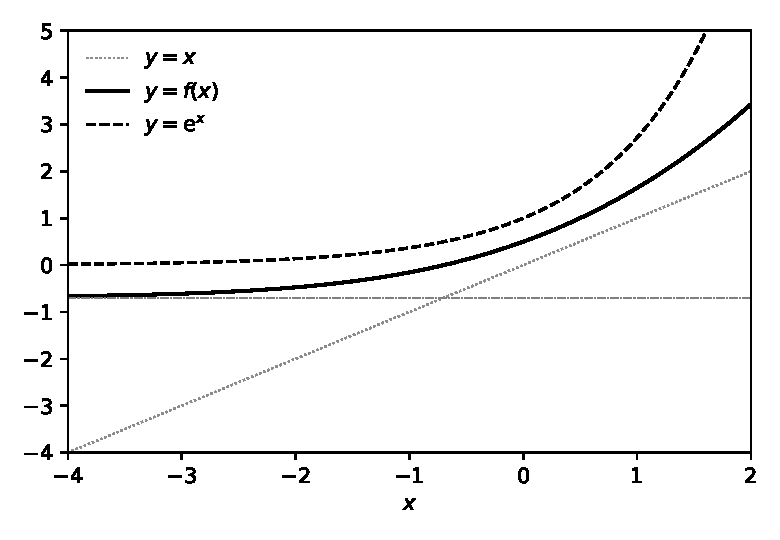
\includegraphics[width=0.62\textwidth]{figures/fig1_halfexp.pdf}
  \caption{Kneser 的半指数函数 $f$（实线）、$\ee^x$（虚线）与对角线。
  点划线是水平渐近线 $y=-0.69602\ldots$。脚本 \texttt{figures/fig1\_halfexp.py}。}
  \label{ch1:fig:halfexp}
\end{figure}

\subsection{Tetration}

与半指数函数等价的问题是解 \textbf{tetration 方程}（超指数方程）
\begin{equation}\label{ch1:eq:tetration}
  F(z+1)=b^{F(z)},\qquad F(0)=1 ,
\end{equation}
这里 $b>1$ 是底数。对正整数 $n$，$F(n)=b^{b^{\cdot^{\cdot^{b}}}}$（$n$ 个 $b$），
所以 $F$ 是把「$n$ 层指数塔」延拓到非整数高度的函数，记作 $\mathrm{sexp}_b$。
若 $\mathrm{sexp}_b$ 是 $\R$ 上（或 $(-2,\infty)$ 上）的严格递增函数，记它的反函数为 $\mathrm{slog}_b$，
则
\[
  f^{\circ t}(x):=\mathrm{sexp}_b\bigl(\mathrm{slog}_b(x)+t\bigr)
\]
满足 $f^{\circ 1}(x)=b^x$ 和 $f^{\circ t}\circ f^{\circ s}=f^{\circ(t+s)}$；取 $t=\frac12$ 就得到 $x\mapsto b^x$ 的半迭代。
对 $b=\ee$，\texttt{kneser} 库给出
\[
  \mathrm{sexp}_\ee(0.5)=1.6463542337511945\ldots,\qquad
  \mathrm{slog}_\ee(10^{300})=3.6367327093389648\ldots .
\]
第二个数说明：$10^{300}$ 这个数只是「3.64 层」的 $\ee$ 指数塔。
Kneser 的半指数函数就是 $f=f^{\circ1/2}=\mathrm{sexp}_\ee\circ(\mathrm{slog}_\ee+\tfrac12)$（$\mathrm{sexp}_\ee$ 取 Kneser 的解）；
\eqref{ch1:eq:halfexp-values} 中 $f(1)=\mathrm{sexp}_\ee(\tfrac12)$ 正是因为 $\mathrm{slog}_\ee(1)=0$。

底数 $b$ 的位置决定了问题的性质。函数 $w\mapsto b^w$ 的实不动点满足 $b^w=w$。
记
\[
  \eta:=\ee^{1/\ee}=1.4446678610\ldots .
\]
\begin{itemize}
\item $b>\eta$ 时，$b^w$ 没有实不动点，只有一对共轭复不动点。$b=\ee$ 时离实轴最近的一对是 $L,\bar L$，$L=0.3181315052\ldots+1.3372357014\ldots\,\ii$。
\item $b=\eta$ 时，$w=\ee$ 是二重不动点，乘子为 $1$（抛物不动点）。
\item $1<b<\eta$ 时，有两个实不动点 $\ee^{\lambda_1}<\ee^{\lambda_2}$，其中 $0<\lambda_1<1<\lambda_2$ 恰好也是它们的乘子（第~\ref{ch:koenigs}~章的例子）。
\end{itemize}
第三种情形是本书的主要舞台。

\begin{example}[底数 $\sqrt2$]\label{ch1:ex:sqrt2}
$b=\sqrt2$ 时 $\sqrt2^{\,2}=2$，$\sqrt2^{\,4}=4$，所以不动点是 $2$ 和 $4$，乘子是
$\lambda_1=2\log\sqrt2=\log2\approx0.693$ 和 $\lambda_2=4\log\sqrt2=2\log2\approx1.386$。
$2$ 是吸引的，$4$ 是排斥的。从 $1$ 出发的轨道
$1,\ \sqrt2,\ \sqrt2^{\sqrt2},\ \dots$ 单调上升收敛到 $2$。
在吸引不动点 $2$ 处，有一个自然的分数次迭代（第~\ref{ch:koenigs}~章的正则解 $R$），由它得到
\[
  \mathrm{sexp}_{\sqrt2}(0.5)=1.2436216276685218\ldots\quad\text{（数值）}.
\]
这个值由脚本 \texttt{figures/ch02\_sqrt2.py} 用 Koenigs 坐标独立算出，
与 \texttt{kneser} 库的 \texttt{sexp} 一致。
$x\to+\infty$ 时 $\mathrm{sexp}_{\sqrt2}(x)$ 从下方趋于 $2$，差按 $\lambda_1^{\,x}=(\log2)^x$ 指数衰减（第~\ref{ch:koenigs}~章）；
例如 $2-\mathrm{sexp}_{\sqrt2}(200)\approx10^{-32}$，在双精度下已不可见。
\end{example}

% ------------------------------------------------------------------
\section{Abel 方程与 Schröder 方程}\label{ch1:sec:abel}

\begin{definition}\label{ch1:def:abel}
设 $f:U\to U$ 是集合 $U$ 到自身的映射。
\begin{enumerate}[label=(\alph*)]
\item 函数 $A:U\to\C$ 若满足
  \begin{equation}\label{ch1:eq:abel}
    A(f(x))=A(x)+1\qquad(x\in U),
  \end{equation}
  则称为 $f$ 的 \textbf{Abel 函数}（Abel function），\eqref{ch1:eq:abel} 称为 \textbf{Abel 方程}。
\item 函数 $F$ 若满足 $F(z+1)=f(F(z))$（在 $F$ 的定义域内），则称为 $f$ 的\textbf{超函数}（superfunction）。
  $A$ 是双射时，$F=A^{-1}$ 就是超函数。
\item 给定 $\lambda\ne0$，函数 $\sigma$ 若满足
  \begin{equation}\label{ch1:eq:schroder}
    \sigma(f(x))=\lambda\,\sigma(x),
  \end{equation}
  则称为 \textbf{Schröder 函数}（Schröder function），\eqref{ch1:eq:schroder} 称为 \textbf{Schröder 方程}。
\end{enumerate}
\end{definition}

Abel 方程把 $f$ 变成平移 $t\mapsto t+1$，Schröder 方程把 $f$ 变成乘法 $\zeta\mapsto\lambda\zeta$。
两者通过对数相联系：若 $\sigma$ 满足 \eqref{ch1:eq:schroder}，且 $\log\sigma$ 的某个分支沿 $f$ 连续，则
\begin{equation}\label{ch1:eq:abel-from-schroder}
  A=\frac{\log\sigma}{\log\lambda}
\end{equation}
满足 $A\circ f=A+1$（对数的分支差一个 $2\pi\ii k/\log\lambda$，见第~\ref{ch:koenigs}~章）。

\begin{definition}[分数次迭代]\label{ch1:def:fractional}
设 $I\subset\R$ 是区间，$f:I\to I$，$A:I\to\R$ 是连续、严格单调的满射并满足 \eqref{ch1:eq:abel}。
对 $t\in\R$，定义
\[
  f_A^{\circ t}:=A^{-1}\circ(A+t)\ :\ I\to I .
\]
称 $\{f_A^{\circ t}\}_{t\in\R}$ 为由 $A$ 确定的\textbf{分数次迭代}（fractional iteration），
$f_A^{\circ1/2}$ 为 $f$ 的一个\textbf{半迭代}。
\end{definition}

\begin{proposition}\label{ch1:prop:flow}
在 \cref{ch1:def:fractional} 的条件下，$f_A^{\circ0}=\id$，$f_A^{\circ1}=f$，
$f_A^{\circ t}\circ f_A^{\circ s}=f_A^{\circ(t+s)}$，并且 $(t,x)\mapsto f_A^{\circ t}(x)$ 连续。
\end{proposition}

\begin{proof}
$A$ 是 $I$ 到 $\R$ 的同胚，所以 $f_A^{\circ t}$ 有定义且连续地依赖于 $(t,x)$。
由 \eqref{ch1:eq:abel}，$A(f(x))=A(x)+1$，即 $f=A^{-1}\circ(A+1)=f_A^{\circ1}$。
群律是 $A^{-1}(A(A^{-1}(A(x)+s))+t)=A^{-1}(A(x)+s+t)$。
\end{proof}

\begin{example}\label{ch1:ex:elementary}
\begin{enumerate}[label=(\arabic*)]
\item $f(x)=2x$，$I=(0,\infty)$。$\sigma(x)=x$ 满足 Schröder 方程（$\lambda=2$），$A(x)=\log_2x$ 是 Abel 函数，
  $f_A^{\circ t}(x)=2^tx$。
\item $f(x)=x^2$，$I=(1,\infty)$。$\sigma(x)=\log x$ 满足 $\sigma\circ f=2\sigma$，
  $A(x)=\log_2\log x$，$f_A^{\circ t}(x)=x^{2^t}$；半迭代是 $x^{\sqrt2}$。
\item $f(x)=x+1$，$I=\R$。$A(x)=x$，$f_A^{\circ t}(x)=x+t$。
\end{enumerate}
\end{example}

在这三个例子里，答案「显然」是唯一的。下一节说明这只是错觉。

% ------------------------------------------------------------------
\section{不唯一性}\label{ch1:sec:nonunique}

\begin{proposition}\label{ch1:prop:nonunique}
设 $f:I\to I$，$A:I\to\R$ 是满足 \eqref{ch1:eq:abel} 的连续严格单调满射。
\begin{enumerate}[label=(\alph*)]
\item 若 $\theta:\R\to\R$ 是 1-周期函数，则 $A_\theta:=A+\theta\circ A$ 也满足 Abel 方程 \eqref{ch1:eq:abel}。
  若 $\theta$ 连续可微且 $\theta'>-1$，则 $A_\theta$ 仍是连续、严格单调的满射，单调方向与 $A$ 相同。
\item 反之，若 $B:I\to\R$ 是 $f$ 的任一 Abel 函数，则存在唯一的 1-周期函数 $\theta$ 使 $B=A+\theta\circ A$。
\item 设 $B=A+\theta\circ A$ 也是连续严格单调满射。则 $f_B^{\circ t}=f_A^{\circ t}$ 对一切 $t\in\R$ 成立，当且仅当 $\theta$ 是常数。
\end{enumerate}
\end{proposition}

\begin{proof}
(a) $A_\theta(f(x))=A(x)+1+\theta(A(x)+1)=A(x)+1+\theta(A(x))=A_\theta(x)+1$。
若 $\theta'>-1$，则 $\varphi:=\id+\theta$ 严格递增；$\theta$ 连续且 1-周期，所以有界，$\varphi(y)-y$ 有界，
于是 $\varphi:\R\to\R$ 是递增满射。$A_\theta=\varphi\circ A$ 因此是连续满射，单调方向与 $A$ 相同。

(b) 令 $\varphi:=B\circ A^{-1}:\R\to\R$，$\theta:=\varphi-\id$。对 $y\in\R$ 令 $x=A^{-1}(y)$。
由 $A(f(x))=y+1$ 得 $A^{-1}(y+1)=f(x)$，于是
\[
  \theta(y+1)=B(f(x))-y-1=B(x)+1-y-1=\theta(y).
\]
所以 $\theta$ 是 1-周期的，且 $B=\varphi\circ A=A+\theta\circ A$。唯一性是因为 $A$ 是满射。

(c) 记 $\varphi=\id+\theta$，它是 $\R$ 上的严格单调满射（因为 $A$、$B$ 都是）。
$f_B^{\circ t}=A^{-1}\circ\varphi^{-1}\circ(\varphi\circ A+t)$。
所以 $f_B^{\circ t}=f_A^{\circ t}$ 对一切 $t$ 成立当且仅当 $\varphi^{-1}(\varphi(y)+t)=y+t$ 对一切 $y,t$ 成立，
即 $\varphi(y+t)=\varphi(y)+t$。取 $y=0$ 得 $\varphi(t)=t+\varphi(0)$，即 $\theta\equiv\varphi(0)$。反之显然。
\end{proof}

\begin{example}[平移的非平凡半迭代]\label{ch1:ex:translation}
取 $f(x)=x+1$，$A(x)=x$，$\theta(y)=\frac{\epsilon}{2\pi}\sin2\pi y$，$|\epsilon|<1$。
则 $A_\theta(x)=x+\frac{\epsilon}{2\pi}\sin2\pi x$ 是实解析、严格递增的 Abel 函数，
它给出的半迭代 $f_{A_\theta}^{\circ1/2}$ 也是实解析的，但当 $\epsilon\ne0$ 时不等于 $x\mapsto x+\frac12$。
事实上，$y=f_{A_\theta}^{\circ1/2}(\tfrac14)$ 是方程 $A_\theta(y)=A_\theta(\tfrac14)+\tfrac12=\tfrac34+\frac{\epsilon}{2\pi}$ 的唯一解，
而 $A_\theta(\tfrac34)=\tfrac34-\frac{\epsilon}{2\pi}$，所以 $\epsilon\ne0$ 时 $f_{A_\theta}^{\circ1/2}(\tfrac14)\ne\tfrac34$。
（在 $x=0$ 处两者碰巧相等，因为 $\sin2\pi y$ 在 $y=0,\frac12$ 处为零。）
\end{example}

\cref{ch1:prop:nonunique} 说明：\emph{连续性、单调性乃至实解析性都不能确定分数次迭代}。
1-周期函数 $\theta$ 是全部的自由度。要选出一个解，必须加别的条件。
历史上有两类条件。
\begin{itemize}
\item \textbf{不动点处的正则性。} 若 $f$ 在不动点 $u_1$ 处可以线性化，要求 $A$ 在 $u_1$ 附近是 \eqref{ch1:eq:abel-from-schroder} 的形式。第~\ref{ch:koenigs}~章证明：在吸引不动点处，这等价于要求超函数 $F=A^{-1}$ 在一个右半平面上全纯，并且关于 $\Ima z$ 一致地趋于 $u_1$。
  在复平面里看，$\theta$ 是 1-周期全纯函数，非常数时在上半平面或下半平面无界（习题~\ref{ch1:ex:liouville}），这样的条件就把它排除了。
\item \textbf{复域中的整体条件。} Kneser 的解在实轴上没有不动点可用，它的条件是复域中的整体条件：在 $\Ima z\to\pm\infty$ 时趋于一对共轭复不动点，再加上~\cite{TrappmannKouznetsov2011} 关于初始区域的单叶性判据，或~\cite{PaulsenCowgill2017} 关于全纯区域与实对称性的条件。
\end{itemize}

% ------------------------------------------------------------------
\section{两种经典答案}\label{ch1:sec:classical}

\subsection{吸引不动点处的正则迭代}\label{ch1:sec:regular}

设 $f$ 在不动点 $u_1$ 附近全纯，乘子 $\lambda_1=f'(u_1)$ 满足 $0<|\lambda_1|<1$。
Koenigs 定理（\cref{thm:koenigs}）给出 $u_1$ 附近唯一的全纯函数 $\sigma$，$\sigma(u_1)=0$，$\sigma'(u_1)=1$，
$\sigma\circ f=\lambda_1\sigma$。于是在 $u_1$ 附近
\[
  f^{\circ t}:=\sigma^{-1}\circ(\lambda_1^{\,t}\,\sigma)
\]
是一个分数次迭代。对实的 $0<\lambda_1<1$，取实的 $\lambda_1^{\,t}=\ee^{t\log\lambda_1}$；
在 $u_1$ 右侧（$\sigma>0$）它就是由 Abel 函数 $\log\sigma/\log\lambda_1$ 确定的迭代，在左侧（$\sigma<0$）则用 $\log(-\sigma)/\log\lambda_1$。
这叫做 $f$ 在 $u_1$ 处的\textbf{正则迭代}。它的超函数
\[
  R(z)=\sigma^{-1}\bigl(\sigma(u^*)\lambda_1^{\,z}\bigr),\qquad R(0)=u^*,
\]
叫做\textbf{吸引正则解}（\cref{def:regular-solution}）。
\cref{ch1:ex:sqrt2} 的 $\mathrm{sexp}_{\sqrt2}$ 就是 $b^w$ 在 $w=2$ 处的吸引正则解，基点取 $1$（这里直接用 $w$ 作自变量）。
它沿实轴单调上升趋于 $2$；而在复方向上，它有虚周期
\[
  \ii h,\qquad h=\frac{2\pi}{|\log\lambda_1|}=17.1431\ldots\quad(b=\sqrt2),
\]
这个周期在全书中反复出现（\cref{prop:regular-periodic}）。

同样，在排斥不动点 $u_2$（$|\lambda_2|>1$）处对 $f$ 的局部逆用 Koenigs 定理，得到\textbf{排斥正则解} $S$。
对 $b=\sqrt2$，$S$ 把实轴单调递减地映到 $(2,4)$，虚周期为 $\ii h_2$，$h_2=2\pi/\log\lambda_2=19.2361\ldots$。

\subsection{Kneser 的构造}\label{ch1:sec:kneser}

$b=\ee$ 时 $\exp$ 没有实不动点，正则迭代无从谈起。Kneser 的构造~\cite{Kneser1950} 可以概括为下面几步
（仓库 \texttt{references/kneser1950/} 中的中文导读给出了每一步的细节）。
取复不动点 $L=0.318\ldots+1.337\ldots\,\ii$。它对 $\exp$ 是排斥的（乘子 $L$，$|L|=1.3746\ldots>1$），
对 $\log$ 的主分支是吸引的，所以有 Koenigs 坐标 $\chi$，满足 $\chi(\ee^{z})=L\,\chi(z)$；
沿 $\log$ 的反复迭代，$\chi$ 延拓到上半平面的一个区域上，并且在那里单叶。
取对数 $w=\log\chi$，$\exp$ 就变成平移 $w\mapsto w+\Log L=w+L$（主值 $\Log L$ 恰好等于 $L$，因为 $\ee^L=L$）。
这是平移，但平移量是复数 $L$，而不是 $1$。
Kneser 在 $w$ 平面中取一个由基本区域反复平移得到的单连通区域 $\mathfrak B$，它在平移 $w\mapsto w+L$ 下不变，边界来自实轴。
Riemann 映射定理把 $\mathfrak B$ 共形地映到上半平面；平移 $w\mapsto w+L$ 变成上半平面的一个没有内部不动点的自同构，
Kneser 证明它是抛物型的，所以可以把它规范成 $\zeta\mapsto\zeta+1$。
这给出一个 Abel 函数 $\Psi$，$\Psi(\ee^z)=\Psi(z)+1$。共形映射把来自实轴的边界送到实轴上，
由 Schwarz 反射原理，$\Psi$ 跨过实轴实解析延拓并取实值；再用 Abel 方程把它延拓到整条实轴上。
半指数函数就是 $\Psi^{-1}(\Psi(x)+\frac12)$。

用本书的语言说，Kneser 的解在 $\Ima z\to+\infty$ 时趋于 $L$，在 $\Ima z\to-\infty$ 时趋于 $\bar L$：
它的上半部分用 $L$ 处的坐标表示，下半部分用 $\bar L$ 处的坐标表示，两部分沿实轴附近的一条缝粘在一起。
这已经是「缝合两个不动点坐标」的雏形。

\subsection{两者如何衔接}

$b>\eta$ 时没有实不动点，可用的是 Kneser 的解；$1<b<\eta$ 时有吸引正则解 $R_b$。
一个自然的问题是：把 Kneser 的解看成底数 $b$ 的解析函数，绕过 $\eta$ 延拓到 $(1,\eta)$ 上，得到的是不是 $R_b$？
答案是否定的。论文~\cite{KneserPaper} 证明：沿上半 $b$ 平面延拓的 Kneser 族 $\Kkn_b$ 在 $(1,\eta)$ 上的边界值等于一个\textbf{缝合解}（sewing solution）$\Ksew_b$；
至少当 $b$ 充分接近 $\eta$ 时，它与 $R_b$ 的差是指数小的，但不为零（主定理 (i)(ii) 与 $B_1\ne0$）。
在 $b=\sqrt2$ 处有数值结果
\[
  \Ima\Ksew_{\sqrt2}(\tfrac12)=-1.18899697185\times10^{-48}\qquad\text{（数值）},
\]
它与 Paulsen 的 120 位数值 $-1.18899697\times10^{-48}$~\cite[\S6]{Paulsen2019} 在所给的 9 位上一致，符号也一致（\cite{KneserPaper} 引言）。
而 $R_{\sqrt2}$ 在实轴上取实值。差的大小由强迫尺度
\[
  \Lam=\ee^{-2\pi h}=\exp\Bigl(\frac{4\pi^2}{\log\lambda_1}\Bigr)=1.66\times10^{-47}\qquad(b=\sqrt2)
\]
控制。第~\ref{ch:koenigs}~章末尾的算例会用 $R$、$S$ 两个正则解和缝合解的一阶近似重算这个数。

% ------------------------------------------------------------------
\section{中心论点：缝合两个不动点坐标}\label{ch1:sec:thesis}

设 $f$ 是实映射，有两个相邻的实不动点 $u_1<u_2$，$u_1$ 吸引、$u_2$ 排斥（\cref{def:regular-solution}）。
两个不动点各有一个 Koenigs 坐标，各给出一个正则解：
\begin{itemize}
\item 吸引正则解 $R$：$R(z+1)=f(R(z))$，虚周期 $\ii h$。它把射线 $[0,\infty)$ 映到 $u_1$ 左边的区间 $[\ustar,u_1)$，把直线 $\Ima z=h/2$ 映到区间 $(u_1,u_2)$。
\item 排斥正则解 $S$：$S(z+1)=f(S(z))$，虚周期 $\ii h_2$。它把实轴映到 $(u_1,u_2)$。
\end{itemize}
所以在区间 $(u_1,u_2)$ 上，$f$ 同时有两个实解析的分数次迭代：一个在 $u_1$ 处正则，一个在 $u_2$ 处正则。
按 \cref{ch1:prop:nonunique}，它们的 Abel 函数相差一个 1-周期函数 $\theta$。
第~\ref{ch:koenigs}~章证明 $\theta(x)=T(x)-x-\ii h/2$，其中 $T$ 是\textbf{转移映射}（transition map）
\[
  T=R^{-1}\circ S,\qquad T(z+1)=T(z)+1,\qquad T(z)-z=\sum_{n\in\Z}t_n\ee^{2\pi\ii nz}
\]
（\cref{def:transition}）。$b=\sqrt2$ 时 $|t_{\pm1}|=3.6\times10^{-25}$：
两个半迭代在 $(2,4)$ 上相差约 $10^{-25}$（第~\ref{ch:koenigs}~章末尾的算例）。

一个 Kneser 型的解 $K$ 在上半平面用 $R$ 表示、在下半平面用 $S$ 表示：
\[
  K=R\circ(\id+P)\ \ (\Ima z\ \text{充分大}),\qquad K=S\circ(\id+Q)\ \ (-\Ima z\ \text{充分大}),
\]
$P$、$Q$ 是 1-周期的。几何上，这是把 $R$ 的时间坐标里的一个上半圆柱和 $S$ 的时间坐标里的一个下半圆柱，
沿 $T$ 共形地缝在一起。不同的缝法给出不同的解；缝法之间的全部差别都由 $T$ 记录。
这就是全书的中心论点：

\begin{center}
\fbox{\parbox{0.86\textwidth}{\centering
一个映射的分数次迭代不是一个函数，而是一种缝合两个不动点坐标的方式。\\
所有缝法之间的差别，都记录在两个坐标的转移映射里。}}
\end{center}

\noindent 当参数变化使两个不动点在一个鞍结（saddle-node）中合并时，
两个 Koenigs 坐标退化为抛物不动点的两个 Fatou 坐标（第~\ref{ch:fatou}~章），
转移映射（经过适当的平移规范化，精确含义见 \cref{thm:confluence}）收敛到抛物芽的\emph{逆} horn 映射 $\horn^{-1}=\Phiatt\circ\Phirep^{-1}$。
它偏离极限的一阶项是 horn 不变量沿开折方向的导数：切向部分（沿抛物层）是 horn 映射的对数导数，法向部分是芽的一个常数。

% ------------------------------------------------------------------
\section{主定理}\label{ch1:sec:main}

本节陈述全书的主定理。所用的记号在后面各章才严格定义，这里先粗略说明。
\begin{itemize}
\item \textbf{实鞍结开折}（\cref{def:unfolding}）：在以鞍结点 $w^*$ 为中心的仿射坐标 $u$（$w=w^*+c\,u$，$c>0$）中，
  $f_s=g-sX+O(s^2)$，其中 $g(u)=u+a_2u^2+a_3u^3+\cdots$（$a_2>0$）是抛物芽，
  $X=-\partial_sf_s|_{s=0}$ 是开折方向，$\gamma=X(0)>0$。$s>0$ 充分小时 $f_s$ 有吸引不动点 $u_1<0$ 和排斥不动点 $u_2>0$，乘子 $0<\lambda_1<1<\lambda_2$。
  条件 (H1)--(H4) 是：$f_s(w)$ 对 $w$ 整、对 $(s,w)$ 联合全纯、实对实（H1）；$w^*$ 是 $f_0$ 的二重不动点，$a_2>0$（H2）；$\gamma>0$（H3）；
  基点 $w_0<w^*$ 满足：$f_0$ 在 $[w_0,w^*]$ 上递增，在 $[w_0,w^*)$ 上 $f_0(w)>w$（H4）。基点在 $u$ 坐标中记作 $\ustar<0$。
  条件 (H5) 是 $B_1\ne0$；涉及第 $n$ 个系数的对数陈述还要求 $B_n\ne0$。
\item 两个正则解 $R$、$S$（\cref{def:regular-solution}），$R(0)=w_0$（$u$ 坐标中是 $\ustar$）；转移映射 $T=R^{-1}\circ S$ 的 Fourier 系数 $t_n$，取在 $\Ima t_0=h/2$ 的分支上；
  \textbf{规范化转移系数} $\tau_n=t_n\ee^{-2\pi\ii nt_0}$。
\item 强迫尺度 $\Lam=\exp(4\pi^2/\log\lambda_1)$；内蕴参数 $p=-\log\lambda_1\cdot\log\lambda_2=4a_2\gamma s+O(s^2)$。
\item 抛物芽 $g$ 的 Fatou 坐标 $\Phiatt,\Phirep$，用形式 Abel 函数 $\alpha(u)=-1/(a_2u)+\rho\log(-u)+\cdots$ 归一化（\cref{def:formal-abel}）；
  逆 horn 映射 $\horn^{-1}(z)=z+\sum_{n\ge1}B_n\ee^{2\pi\ii nz}$（\cref{def:horn}）；基点的 Fatou 值 $a=\Phiatt(\ustar)$。
\end{itemize}

\begin{theorem}[主定理]\label{thm:main-preview}
设 $f_s=g-sX+O(s^2)$ 是满足 \textup{(H1)--(H4)} 的实鞍结开折（\cref{def:unfolding}），$s\downarrow0$。则对每个 $n\ge1$：
\begin{enumerate}[label=\textup{(\roman*)},leftmargin=2.2em]
\item \textbf{缝合}（\cref{thm:sewing}）。$s>0$ 充分小时，存在一个解 $\Ksew_s$（$\Ksew_s(z+1)=f_s(\Ksew_s(z))$，$\Ksew_s(0)=w_0$），
  它是满足缝口高度条件的类（\cref{def:class}）中唯一的元素（\cref{thm:characterization}），它的分离系数 $c_n$（$\Ksew_s=R\circ(\id+\sum_{n\ge0}c_n\ee^{2\pi\ii nz})$）满足
  \[
    \frac{c_n}{\Lam^n}=\tau_n+O(\Lam).
  \]
\item \textbf{汇流}（\cref{thm:confluence}）。$\tau_n\to B_n\ee^{2\pi\ii na}$。
\item \textbf{展开}（\cref{thm:all-orders}）。若 $B_n\ne0$（(H5) 对第 $n$ 个系数的要求），则 $\log\bigl(\tau_n/B_n\ee^{2\pi\ii na}\bigr)$ 有渐近展开
  \[
    \log\frac{\tau_n}{B_n\ee^{2\pi\ii na}}\sim\sum_{j\ge1}\kappa^{(n)}_jp^j,\qquad p=-\log\lambda_1\cdot\log\lambda_2,
  \]
  各系数 $\kappa^{(n)}_j$ 由抛物芽 $g$（及其反射逆）轨道上的收敛级数给出。
\item \textbf{变分}（\cref{thm:variation}）。若 $B_n\ne0$，则
  \[
    \kappa^{(n)}_1=\ktr^{(n)}(g)+\frac{\Dfun_n(g)\bigl[X-X(0)\bigr]}{4a_2X(0)},
  \]
  其中 $\ktr^{(n)}(g)$ 是平移开折 $g-s$ 的一阶系数，$\Dfun_n=\dd\log(B_n\ee^{2\pi\ii na})$ 是沿抛物层 $\Pstr$ 的对数微分。
\item \textbf{不变性}（\cref{prop:base-point}、\cref{cor:invariance}）。$|\tau_n|$ 与 $\Rea\kappa^{(n)}_j$ 不依赖基点的选取，
  并且是开折在局部保向实解析共轭下的不变量。
\end{enumerate}
\end{theorem}

各条的出处（按论文 PDF 中的编号；括号内是 \texttt{main.tex}、\texttt{sec-general.tex} 中的标签）：
(i) 是 \cite[Thm.~B、Thm.~8.2 及一般形式 Thm.~9.3]{KneserPaper}（\texttt{mthm:B}、\texttt{thm:char}、\texttt{thm:gen-B}）；
(ii) 是 \cite[Thm.~A 及 Thm.~9.2]{KneserPaper}（\texttt{mthm:A}、\texttt{thm:gen-A}）；
(iii) 是 \cite[Thm.~C、Thms.~5.6、5.8 及 Thm.~9.4]{KneserPaper}（\texttt{mthm:D}、\texttt{thm:D}、\texttt{thm:E}、\texttt{thm:gen-D}）；
(iv) 是 \cite[Thm.~9.10]{KneserPaper}（\texttt{thm:gen-variation}）；(v) 是 \cite[Prop.~9.6、Cor.~9.7]{KneserPaper}（\texttt{prop:gen-base}、\texttt{cor:gen-invariant}）。
(i)--(v) 在本书中都有完整证明（第~\ref{ch:transition}--\ref{ch:variation}~章）。
论文另外对 (iv) 做了数值检验：$n=1$ 时两边相差约 $3\times10^{-17}$（$n=2,3$ 时分别约为 $2\times10^{-13}$、$3\times10^{-9}$）。这是数值事实，不是证明的一部分。

\begin{remark}[读法]\label{ch1:rem:reading}
主定理的各条按「阶」排列。
零阶：$|B_n|$ 只依赖芽 $g$，是 Écalle--Voronin 模的模长；$B_n\ee^{2\pi\ii na}$ 依赖芽和基点，是汇流的极限。
一阶：$\Rea\kappa^{(n)}$ 依赖开折方向 $X$；(iv) 说它分成只依赖芽的法向部分 $\Rea\ktr^{(n)}(g)$ 和 horn 映射的切向导数。
高阶：$\Rea\kappa^{(n)}_j$ 由同一类收敛级数构造。
(i) 把这些量和一个具体的解 $\Ksew_s$ 联系起来：分离系数 $c_n$ 是 $\Lam^n\tau_n$ 加上相对误差 $O(\Lam)$。
\end{remark}

\begin{example}[tetration]\label{ch1:ex:tetration-data}
对 $b^w$，在坐标 $w=\ee(1+u)$ 中鞍结芽是 $g(u)=\ee^u-1$，$a_2=\frac12$，$\rho=\frac13$，
开折参数 $s=1-\ee\log b$，$\gamma=1$，$p=2s+O(s^2)$，基点 $w_0=1$ 即 $\ustar=1/\ee-1$。
\cite[\S2.1 与 Prop.~2.6]{KneserPaper} 给出
\[
  |B_1|=0.0890584364122133\ldots,\qquad a=3.0292972144180\ldots ,
\]
两者都有区间算术证书（第~\ref{ch:fatou}~章）。主定理 (ii) 说 $\tau_1\to B_1\ee^{2\pi\ii a}$。
在 $b=\sqrt2$（离 $\eta$ 并不很近）处，
脚本 \texttt{figures/ch02\_sqrt2.py} 算出 $|\tau_1|=0.0889497\ldots$（数值），与 $|B_1|$ 只相差约 $0.12\%$。
\end{example}

% ------------------------------------------------------------------
\section{全书路线图}\label{ch1:sec:roadmap}

全书分四部分。
\begin{itemize}
\item \textbf{两类不动点}（第~\ref{ch:koenigs}、\ref{ch:fatou}~章）。第~\ref{ch:koenigs}~章是双曲不动点的 Koenigs 理论和两个正则解 $R$、$S$；
  第~\ref{ch:fatou}~章是抛物不动点的 Fatou 坐标、horn 映射和 $B_1\ne0$。
\item \textbf{双坐标理论}（第~\ref{ch:unfolding}--\ref{ch:sewing}~章）。第~\ref{ch:unfolding}~章给出实鞍结开折的定义与尺度；
  第~\ref{ch:transition}~章定义转移映射并证明焊接恒等式和基点无关性；
  第~\ref{ch:sewing}~章构造缝合解并证明它的刻画定理。
\item \textbf{汇流与展开}（第~\ref{ch:confluence}--\ref{ch:variation}~章）。第~\ref{ch:confluence}~章证明汇流定理；
  第~\ref{ch:first-order}~章给出一阶项和全阶展开；第~\ref{ch:variation}~章证明变分公式。
\item \textbf{例子、数值与开放问题}（第~\ref{ch:examples}--\ref{ch:open}~章）。第~\ref{ch:examples}~章讲 tetration 及其他族，
  包括 Kneser 解绕过尖点 $\eta$ 的延拓；第~\ref{ch:numerics}~章讲数值方法；第~\ref{ch:open}~章列出开放问题。
\end{itemize}
附录~\ref{app:tools} 收集复分析工具（Weierstrass 预备定理、可测 Riemann 映射定理等），附录~\ref{app:notation} 是记号表。
各章的逻辑依赖如下（箭头表示「被用于」）：
\[
\begin{tikzcd}[column sep=1.6em,row sep=1.4em]
 & \text{第 2 章} \ar[d] & \text{第 4 章}\ar[dl]\ar[dr] & \text{第 3 章}\ar[d]\ar[ddr,bend left=20] & \\
 & \text{第 5 章}\ar[dl]\ar[rr] & & \text{第 7 章}\ar[d]\ar[dll] & \\
 \text{第 6 章}\ar[r] & \text{第 10 章} & & \text{第 8 章}\ar[r] & \text{第 9 章}
\end{tikzcd}
\]
图中只画了主要的证明依赖；例如第~\ref{ch:sewing}~章关于 $c_n/\Lam^n$ 极限的推论还用到第~\ref{ch:confluence}~章的汇流定理。
第~\ref{ch:numerics}~章用到前面所有各章，第~\ref{ch:open}~章不被其他章引用。
只想了解主线的读者可以按 $2\to4\to5\to6$ 读到缝合解，再按 $3\to7\to8\to9$ 读到变分公式。

% ------------------------------------------------------------------
\notes

\paragraph{函数方程。}
Abel 方程与 Schröder 方程以 N.~H.~Abel 和 E.~Schröder~\cite{Schroder1870} 命名。
Koenigs 1884 年证明了双曲不动点处 Schröder 方程解的存在唯一性~\cite{Koenigs1884}，这是第~\ref{ch:koenigs}~章的主题；
Fatou 在 1919 年的长文中研究了抛物不动点处的 Abel 方程~\cite{Fatou1919}。
\cref{ch1:prop:nonunique} 属于文献中的常识（folklore），在关于分数次迭代的文献中反复出现；
它说明，任何关于「自然」分数迭代的唯一性定理，都必须是一个关于 1-周期函数 $\theta$ 的 Liouville 型定理。

\paragraph{Kneser 与 tetration。}
Kneser 1950 年的论文~\cite{Kneser1950} 构造了 $\varphi(\varphi(x))=\ee^x$ 的实解析解。
仓库目录 \texttt{references/kneser1950/} 有这篇论文的中文导读。
Kouznetsov~\cite{Kouznetsov2009} 在复平面上高精度地计算了 $\ee$ 底的超指数；
Kouznetsov 与 Trappmann 研究了底数 $\sqrt2$ 的正则超指数~\cite{KouznetsovTrappmann2010}
和底数 $\ee^{1/\ee}$ 的两个正则超指数~\cite{KouznetsovTrappmann2012}；
Trappmann 与 Kouznetsov 给出了复不动点对处全纯 Abel 函数的唯一性判据，并证明 Kneser 的解满足它~\cite{TrappmannKouznetsov2011}。
Paulsen 与 Cowgill~\cite{PaulsenCowgill2017} 证明了实底数 $b>\eta$ 的唯一性定理并给出高精度算法；
Paulsen~\cite{Paulsen2019} 提出沿底数把 Kneser 的构造延拓到复底数，并穿过 Shell--Thron 区域。
\cite[引言中关于 Paulsen 2019 的注]{KneserPaper} 指出，\cite[Prop.~2]{Paulsen2019} 的唯一性陈述按原文对每个实 $b>\eta$ 都不成立，复底数还需要一个选根条件；
Shell--Thron 边界的穿越在~\cite{Paulsen2019} 中是用数值论证的，\cite{KneserPaper} 的定理 D、E（源文件标签 \texttt{mthm:F}、\texttt{mthm:G}；定理 E 是计算机辅助的）给出了证明（第~\ref{ch:examples}~章）。
Paulsen 后来又分析了 $z\uparrow\uparrow a$ 对分数 $a$ 的性质~\cite{Paulsen2026}。
Nixon~\cite{Nixon2022} 用无穷复合构造了 Shell--Thron 区域内部的非正则解，并用 1-周期的「$\theta$ 映射」把它们与正则解比较，
这与本书的写法 $K=R\circ(\id+P)$ 相同；但那里没有转移映射、horn 映射和 $b\to\eta$ 的极限（见 \texttt{docs/prior-art-check-zh.md}）。

\paragraph{抛物点与汇流。}
抛物芽的解析分类由 Écalle~\cite{Ecalle1981} 和 Voronin~\cite{Voronin1981} 完成，分类的不变量就是 horn 映射（第~\ref{ch:fatou}~章）。
开折时两个不动点有两种分裂方式。两个不动点是共轭复数时，Fatou 坐标的极限由抛物内爆（parabolic implosion）描述，
这是 Lavaurs~\cite{Lavaurs1989}、Shishikura~\cite{Shishikura2000}、Oudkerk~\cite{Oudkerk1999} 的工作；本书称之为 Lavaurs 方向。
两个不动点都是实数时，Glutsyuk~\cite{Glutsyuk2001} 研究了不动点汇合时的非线性 Stokes 现象，证明了开折的解析分类模在这一方向上收敛到抛物芽的 Écalle--Voronin 模；
Mardešić、Roussarie、Rousseau~\cite{MRR2004} 构造了开折的解析分类模，并证明它在参数为 $0$ 处连续；
Christopher 与 Rousseau~\cite{ChristopherRousseau} 证明了模关于规范参数的 $\frac12$-可和性，不可和方向正是 Glutsyuk 方向；
Ribón~\cite{Ribon2010} 把可和性推广到有限余维的开折。向量场的情形见~\cite{RousseauTeyssier2008}。
这些结果（在各自的规范下）给出了主定理 (iii) 中渐近展开的\emph{存在性}，但没有给出系数；本书（与 \cite{KneserPaper}）给出的是系数的收敛级数表示与一个不用可和性理论的直接证明，
以及 (iv) 的变分公式。用收敛级数表示 Écalle--Voronin 不变量的做法见~\cite{DudkoSauzin2014}；
在抛物族内部（不动点不分裂）对 horn 映射作参数展开，见~\cite[Prop.~9.1]{BuffEcalleEpstein2013}。

\paragraph{一个相邻领域。}
保面积映射在鞍--中心分岔附近的分界线分裂（separatrix splitting）有同样形状的结果：
同宿不变量是 $\ee^{-2\pi^2/\log\lambda}$ 乘以一个参数的渐近级数，首项是抛物极限的 Stokes 常数~\cite{GelfreichBrannstrom,GelfreichSauzin2001}，
高阶系数可以高精度地数值提取~\cite{GelfreichSimo2008}。那里只有一个 Fourier 模，对象是二维映射。

\paragraph{本书与论文。}
本书的理论来源是论文~\cite{KneserPaper}。论文以 tetration 为主线，一般开折在其 \S9 ``General real saddle-node unfoldings''（\texttt{sec-general.tex}）中给出；
本书反过来，以一般实鞍结开折为主线，tetration 是第一个例子。
仓库中的 Lean~4 工程（\texttt{lean/}）对实际指数族形式化了主定理 (i)--(iii) 的对应部分；(iv) 尚未形式化。

% ------------------------------------------------------------------
\exercises

\begin{exercise}\label{ch1:ex:increasing}
设 $f:\R\to\R$ 连续，$f\circ f=\exp$。证明 $f$ 严格递增，且 $x<f(x)<\ee^x$ 对一切实数 $x$ 成立。
\end{exercise}
\begin{hint}
单射加连续推出严格单调。若 $f$ 递减，考虑 $f(x)-x$ 在 $\pm\infty$ 处的符号并用介值定理得到不动点。
$f(x)>x$：否则由介值定理 $f$ 有不动点。$f(x)<\ee^x$：对 $y=f(x)$ 用 $f(y)>y$。
\end{hint}

\begin{exercise}\label{ch1:ex:asymptote}
设 $f$ 是 \cref{ch1:ex:increasing} 中的函数。证明 $c:=\lim_{x\to-\infty}f(x)$ 存在且有限，$f(c)=0$，$f(0)=\ee^{c}$。
用 \eqref{ch1:eq:halfexp-values} 中 Kneser 解的数值 $f(0)=0.4985632879\ldots$ 与 $c=-0.6960247408\ldots$ 检验最后一个等式。
\end{exercise}

\begin{exercise}
对 $f(x)=x^2$（$x>1$）验证 \cref{ch1:ex:elementary}(2)，并写出由 $\theta(y)=\epsilon\sin2\pi y$（$0<|\epsilon|<1/(2\pi)$）给出的另一个半迭代 $f_\theta^{\circ1/2}$。
证明 $f_\theta^{\circ1/2}(\ee)=\ee^{\sqrt2}$，但 $f_\theta^{\circ1/2}(\ee^{2^{1/4}})\ne\ee^{2^{3/4}}$。
\end{exercise}

\begin{exercise}\label{ch1:ex:flow-to-abel}
设 $I$ 是区间，$\{f^t\}_{t\in\R}$ 是 $I$ 上的连续流（$f^0=\id$，$f^t\circ f^s=f^{t+s}$，$(t,x)\mapsto f^t(x)$ 连续），
$f^1=f$，并且对某个 $x_0\in I$，$t\mapsto f^t(x_0)$ 是 $\R$ 到 $I$ 的严格递增满射。
证明 $A(x):=$「使 $f^t(x_0)=x$ 的 $t$」是 $f$ 的 Abel 函数，且 $f^t=f_A^{\circ t}$。
所以 \cref{ch1:def:fractional} 涵盖了所有这样的流。
\end{exercise}

\begin{exercise}
设 $\sigma:I\to(0,\infty)$ 是连续、严格单调的满射，并且是 $f:I\to I$ 的 Schröder 函数，$\sigma\circ f=\lambda\sigma$，$0<\lambda\ne1$。
证明 $A=\log\sigma/\log\lambda$ 满足 \cref{ch1:def:fractional} 的条件，并且由 $A$ 确定的分数次迭代是 $\sigma^{-1}(\lambda^t\sigma)$。
若 $\tilde\sigma=c\sigma$（$c>0$），分数次迭代是否改变？若 $\tilde\sigma=\sigma^2$ 呢？
\end{exercise}

\begin{exercise}\label{ch1:ex:liouville}
设 $\theta$ 是 1-周期的整函数。证明：若 $\theta$ 在上半平面 $\{\Ima z>0\}$ 上有界，则 $\theta(z)=\sum_{n\ge0}\theta_n\ee^{2\pi\ii nz}$；
若它在上、下两个半平面都有界，则 $\theta$ 是常数。由此说明 \cref{ch1:sec:nonunique} 末尾所说的「复域条件」为什么能排除自由度 $\theta$。
\end{exercise}
\begin{hint}
令 $q=\ee^{2\pi\ii z}$，$\theta(z)=\Theta(q)$，$\Theta$ 在 $\C^*$ 上全纯。$\Ima z\to+\infty$ 对应 $q\to0$，用 Riemann 可去奇点定理。
\end{hint}

\begin{exercise}
对 $b\in(1,\eta)$，证明 $w\mapsto b^w$ 恰有两个实不动点，并且从任何 $w_0<\ee^{\lambda_1}$ 出发的轨道单调收敛到较小的不动点 $\ee^{\lambda_1}$。
对 $b=\sqrt2$ 直接验证不动点是 $2$ 和 $4$。
\end{exercise}

\begin{exercise}\label{ch1:ex:two-half}
（本题预告第~\ref{ch:koenigs}~章。）设 $f$ 在区间 $[u_1,u_2]$ 上实解析、严格递增，$f(u_j)=u_j$，$f(u)<u$ 于 $(u_1,u_2)$，
$0<\lambda_1=f'(u_1)<1<\lambda_2=f'(u_2)$。设 $\sigma$、$\sigma_{\mathrm{rep}}$ 是两端的 Koenigs 坐标（\cref{thm:koenigs}）沿 $f$ 延拓到 $(u_1,u_2)$。
证明 $\sigma>0$、$\sigma_{\mathrm{rep}}<0$ 于 $(u_1,u_2)$，从而 $A_1=\log\sigma/\log\lambda_1$ 与 $A_2=\log(-\sigma_{\mathrm{rep}})/\log\lambda_2$ 都是 $(u_1,u_2)$ 上的实 Abel 函数。
假定它们都是 $(u_1,u_2)$ 到 $\R$ 的满射（第~\ref{ch:koenigs}~章证明了这一点），用 \cref{ch1:prop:nonunique}(c) 说明：两者对一切 $t$ 给出相同的分数次迭代，当且仅当 $A_1-A_2$ 是常数。
只要求半迭代相同时，条件是什么？
\end{exercise}

\begin{exercise}
（较难）设 $f$ 同 \cref{ch1:ex:two-half}，并设 $f$ 是 Möbius 变换 $f(u)=u/(2-u)$，$u_1=0$，$u_2=1$。
证明此时 $A_1-A_2$ 是常数。所以对 Möbius 变换，两个不动点给出同一个分数次迭代。
\end{exercise}
\begin{hint}
$y=u/(1-u)$ 把 $f$ 共轭成 $y\mapsto y/2$。两个 Koenigs 坐标分别是 $y$ 与 $-1/y$ 的常数倍。
\end{hint}

% 第 2 章 双曲不动点与 Koenigs 坐标
% 经典部分：Koenigs 1884；Milnor 2006 §8；Carleson--Gamelin Ch. II。
% 本理论部分：[KneserPaper] §2.1（Lemma param）、§3.1（S、R^{-1} 与 Lemma realT）、sec-general.tex（(H4) 的改写）。
% 数值：figures/ch02_sqrt2.py；图：figures/fig2_regular.py。
\chapter{双曲不动点与 Koenigs 坐标}\label{ch:koenigs}

本章讲两个不动点中「容易」的那一类：乘子 $\lambda$ 满足 $|\lambda|\ne0,1$ 的不动点。
在这样的不动点附近，映射可以全纯地共轭成乘法 $\zeta\mapsto\lambda\zeta$（Koenigs 定理），
共轭坐标在相差常数倍的意义下唯一。对它取对数再除以 $\log\lambda$，就得到 Abel 坐标；
它的逆是一个超函数，即「正则迭代」。

本章后半部分把这些经典事实用到一个具体设定上：实轴上的实映射 $f$，有相邻的吸引不动点 $u_1$ 和排斥不动点 $u_2$。
两个不动点各给出一个超函数，记作 $R$ 和 $S$（\cref{def:regular-solution}）。
它们是全书的两块基本材料：第~\ref{ch:transition}~章用它们定义转移映射，第~\ref{ch:sewing}~章把它们缝起来。
本章的例子是 $b^w$（$1<b<\eta$），算例取 $b=\sqrt2$。

\begin{goals}
\item Koenigs 线性化定理（\cref{thm:koenigs}）的完整证明，以及 Schröder 映射在相差常数倍意义下的唯一性（\cref{ch2:cor:schroder-unique}）。
\item 吸引不动点的 Koenigs 坐标沿函数方程延拓到整个吸引域；排斥不动点的 Poincaré 函数延拓为整函数（\cref{ch2:prop:extend,ch2:prop:poincare}）。
\item 实映射的两个正则解 $R$、$S$（\cref{def:regular-solution}）：它们有虚周期 $\ii h$、$\ii h_2$，在实轴上有确定的实结构（\cref{prop:regular-periodic}），并由「在半平面上一致收敛到不动点」刻画（\cref{ch2:prop:regular-unique}）。
\item $R$ 与 $S$ 在区间 $(u_1,u_2)$ 上给出两个不同的实解析分数次迭代；它们的差就是第~\ref{ch:transition}~章的转移映射。$b=\sqrt2$ 时两者相差约 $10^{-25}$（\cref{ch2:ex:sqrt2-transition}）。
\end{goals}

% ==================================================================
\section{线性化问题}\label{ch2:sec:linearization}

设 $f$ 在点 $p$ 的邻域内全纯，$f(p)=p$。称 $\lambda:=f'(p)$ 为不动点 $p$ 的\textbf{乘子}（multiplier）。按 $\lambda$ 分类：
\begin{itemize}
\item $\lambda=0$：\textbf{超吸引}（superattracting）；
\item $0<|\lambda|<1$：\textbf{吸引}（attracting）；
\item $|\lambda|>1$：\textbf{排斥}（repelling）；
\item $|\lambda|=1$：\textbf{中性}（neutral），其中 $\lambda$ 为单位根时称为\textbf{抛物}（parabolic）。
\end{itemize}
本章处理 $0<|\lambda|<1$ 与 $|\lambda|>1$ 两种情形，统称\textbf{双曲}（hyperbolic）不动点。
抛物情形 $\lambda=1$ 是第~\ref{ch:fatou}~章的主题。

\textbf{线性化问题}是：是否存在 $p$ 附近的全纯函数 $\sigma$，$\sigma(p)=0$，$\sigma'(p)=1$，使
\begin{equation}\label{ch2:eq:schroder}
  \sigma\circ f=\lambda\,\sigma .
\end{equation}
这就是第~\ref{ch:intro}~章的 Schröder 方程，满足它的 $\sigma$ 称为 \textbf{Schröder 映射}（Schröder map）或 \textbf{Koenigs 坐标}（Koenigs coordinate）。
若 $\sigma$ 存在，则它在 $p$ 附近单叶，并且 $f=\sigma^{-1}\circ(\lambda\,\cdot)\circ\sigma$：在坐标 $\zeta=\sigma(u)$ 中，$f$ 就是乘以 $\lambda$。

先看形式层面。不妨设 $p=0$。

\begin{lemma}[形式解]\label{ch2:lem:formal}
设 $f(z)=\lambda z+\sum_{k\ge2}f_kz^k$ 是形式幂级数，$\lambda\ne0$，且 $\lambda^{k-1}\ne1$ 对一切 $k\ge2$ 成立。
则存在唯一的形式幂级数 $\sigma(z)=z+\sum_{k\ge2}s_kz^k$ 使 $\sigma\circ f=\lambda\sigma$。系数由递推
\begin{equation}\label{ch2:eq:recursion}
  (\lambda-\lambda^k)\,s_k=\bigl[z^k\bigr]\Bigl(f(z)+\sum_{j=2}^{k-1}s_j\,f(z)^j\Bigr)\qquad(k\ge2)
\end{equation}
确定，其中 $[z^k]$ 表示取 $z^k$ 的系数。
\end{lemma}

\begin{proof}
$\sigma(f(z))=f(z)+\sum_{j\ge2}s_jf(z)^j$。因为 $f(z)^j=\lambda^jz^j+O(z^{j+1})$，
$z^k$ 的系数中含 $s_k$ 的项只有 $s_k\lambda^k$，其余项只含 $s_2,\dots,s_{k-1}$。
比较 $\sigma\circ f$ 与 $\lambda\sigma$ 的 $z^k$ 系数，得到 $\lambda^ks_k+[z^k](f+\sum_{j<k}s_jf^j)=\lambda s_k$，即 \eqref{ch2:eq:recursion}。
因为 $\lambda-\lambda^k=\lambda(1-\lambda^{k-1})\ne0$，$s_k$ 被唯一确定。
\end{proof}

当 $0<|\lambda|<1$ 或 $|\lambda|>1$ 时，$|\lambda^{k-1}|\ne1$，条件自动成立，并且分母 $|\lambda-\lambda^k|$ 远离零：
$0<|\lambda|<1$ 时 $|\lambda-\lambda^k|\ge|\lambda|(1-|\lambda|)$。这正是收敛的原因。
当 $|\lambda|=1$ 而 $\lambda$ 不是单位根时，分母可以任意小（「小分母」），收敛与否取决于 $\lambda$ 的辐角的算术性质（Siegel、Brjuno、Cremer，见~\cite[\S11]{Milnor2006}）。
当 $\lambda=1$ 时递推在 $k=2$ 就失效：抛物不动点不能线性化，取而代之的是 Fatou 坐标（第~\ref{ch:fatou}~章）。

% ==================================================================
\section{Koenigs 线性化定理}\label{ch2:sec:koenigs}

\begin{theorem}[Koenigs~\cite{Koenigs1884}]\label{thm:koenigs}
设 $f$ 在 $p$ 的邻域内全纯，$f(p)=p$，$\lambda=f'(p)$ 满足 $0<|\lambda|<1$ 或 $|\lambda|>1$。则存在 $p$ 的邻域 $U$ 和 $U$ 上的单叶全纯函数 $\sigma$，使
\[
  \sigma(p)=0,\qquad \sigma'(p)=1,\qquad \sigma(f(u))=\lambda\,\sigma(u)\quad(u\in U\cap f^{-1}(U)).
\]
满足这三个条件的全纯函数芽是唯一的。吸引情形下可以取 $U$ 使 $f(U)\subset U$，并且
\begin{equation}\label{ch2:eq:koenigs-limit}
  \sigma(u)=\lim_{n\to\infty}\lambda^{-n}\bigl(f^{\circ n}(u)-p\bigr)
\end{equation}
在 $U$ 上一致成立。
\end{theorem}

\begin{proof}
不妨设 $p=0$。

\emph{吸引情形 $0<|\lambda|<1$。}
取常数 $c$ 使 $|\lambda|<c<\sqrt{|\lambda|}$（这是可能的，因为 $|\lambda|<1$ 推出 $|\lambda|<\sqrt{|\lambda|}$）。
由 Taylor 展开，存在 $r_0>0$、$C>0$ 使
\begin{equation}\label{ch2:eq:taylor}
  |f(z)-\lambda z|\le C|z|^2\qquad(|z|\le r_0).
\end{equation}
取 $0<r\le r_0$ 使 $|\lambda|+Cr\le c$。则对 $|z|\le r$ 有 $|f(z)|\le(|\lambda|+C|z|)|z|\le c|z|$，
所以 $f$ 把闭圆盘 $\overline D_r=\{|z|\le r\}$ 映入自身，且
\begin{equation}\label{ch2:eq:orbit-bound}
  |f^{\circ n}(z)|\le c^n|z|\qquad(|z|\le r,\ n\ge0).
\end{equation}
令 $\sigma_n(z):=\lambda^{-n}f^{\circ n}(z)$。由 \eqref{ch2:eq:taylor}、\eqref{ch2:eq:orbit-bound}，
\[
  |\sigma_{n+1}(z)-\sigma_n(z)|
  =|\lambda|^{-n-1}\bigl|f(f^{\circ n}(z))-\lambda f^{\circ n}(z)\bigr|
  \le|\lambda|^{-n-1}C\,|f^{\circ n}(z)|^2
  \le\frac{Cr^2}{|\lambda|}\Bigl(\frac{c^2}{|\lambda|}\Bigr)^{n}.
\]
因为 $c^2<|\lambda|$，级数 $\sum_n(\sigma_{n+1}-\sigma_n)$ 在 $\overline D_r$ 上一致收敛，
所以 $\sigma_n$ 一致收敛到 $D_r$ 上的全纯函数 $\sigma$，这就是 \eqref{ch2:eq:koenigs-limit}。
每个 $\sigma_n$ 满足 $\sigma_n(0)=0$、$\sigma_n'(0)=1$，取极限得 $\sigma(0)=0$、$\sigma'(0)=1$。
又 $\sigma_n(f(z))=\lambda\sigma_{n+1}(z)$，取极限得 $\sigma\circ f=\lambda\sigma$ 于 $D_r$。
$\sigma'(0)\ne0$，所以 $\sigma$ 在 $0$ 的某个邻域上单叶；
取 $U$ 为该邻域中的一个小圆盘 $D_{r'}$（$r'\le r$），则 $f(U)\subset U$ 仍成立。

唯一性：设 $\varphi$ 在 $D_\rho$ 上全纯，$\varphi(0)=0$，$\varphi'(0)=1$，并在 $0$ 附近满足 $\varphi\circ f=\lambda\varphi$。
缩小 $r$（上面关于 $r$ 的条件对更小的 $r$ 仍成立），可设 $r\le\rho$，$\varphi\circ f=\lambda\varphi$ 于 $D_r$，并且 $|\varphi(w)-w|\le M|w|^2$（$|w|\le r$）。
因为 $f^{\circ n}(D_r)\subset D_r$，迭代函数方程得 $\varphi=\lambda^{-n}\varphi\circ f^{\circ n}$ 于 $D_r$，于是
\[
  |\varphi(z)-\sigma_n(z)|=|\lambda|^{-n}\bigl|\varphi(f^{\circ n}(z))-f^{\circ n}(z)\bigr|
  \le|\lambda|^{-n}M|f^{\circ n}(z)|^2\le Mr^2\Bigl(\frac{c^2}{|\lambda|}\Bigr)^n\to0 .
\]
所以 $\varphi=\lim\sigma_n=\sigma$ 于 $D_r$。

\emph{排斥情形 $|\lambda|>1$。}
$f'(0)=\lambda\ne0$，所以 $f$ 把 $0$ 的某个邻域 $U_0$ 双全纯地映到 $0$ 的邻域 $V_0$。
记 $\iota:=(f|_{U_0})^{-1}:V_0\to U_0$，则 $\iota(0)=0$，$\iota'(0)=1/\lambda$，$0<|1/\lambda|<1$。
对 $\iota$ 用吸引情形，得到 $0$ 附近的单叶函数 $\sigma$，$\sigma(0)=0$，$\sigma'(0)=1$，$\sigma\circ \iota=\lambda^{-1}\sigma$。
对 $u$ 靠近 $0$，令 $w=f(u)$，则 $\iota(w)=u$，上式给出 $\sigma(u)=\lambda^{-1}\sigma(f(u))$，即 $\sigma\circ f=\lambda\sigma$。
反过来，$0$ 附近满足 $\sigma\circ f=\lambda\sigma$ 的函数也满足 $\sigma\circ \iota=\lambda^{-1}\sigma$，所以唯一性由吸引情形推出。
\end{proof}

\begin{corollary}[Schröder 映射的唯一性]\label{ch2:cor:schroder-unique}
在 \cref{thm:koenigs} 的条件下，设 $\varphi$ 在 $p$ 附近全纯，$\varphi(p)=0$，且 $\varphi\circ f=\lambda\varphi$。则 $\varphi=\varphi'(p)\,\sigma$。
特别地，满足 \eqref{ch2:eq:schroder} 且在 $p$ 处为零的全纯函数，在相差一个常数倍的意义下唯一。
\end{corollary}

\begin{proof}
若 $\varphi'(p)\ne0$，对 $\varphi/\varphi'(p)$ 用 \cref{thm:koenigs} 的唯一性。
若 $\varphi'(p)=0$ 而 $\varphi\not\equiv0$，设 $\varphi(u)=a_m(u-p)^m+O((u-p)^{m+1})$，$m\ge2$，$a_m\ne0$。
比较 $\varphi(f(u))=a_m\lambda^m(u-p)^m+\cdots$ 与 $\lambda\varphi(u)=\lambda a_m(u-p)^m+\cdots$ 的首项，得 $\lambda^{m-1}=1$，与 $|\lambda|\ne1$ 矛盾。
\end{proof}

\begin{remark}[实结构]\label{ch2:rem:real-sigma}
设 $f$ 在实轴上取实值（即 $f(\bar u)=\overline{f(u)}$），$p$ 与 $\lambda$ 为实数。
则 $\tilde\sigma(u):=\overline{\sigma(\bar u)}$ 也满足 \cref{thm:koenigs} 的三个条件，由唯一性 $\tilde\sigma=\sigma$。
所以 $\sigma$ 在实轴上取实值。若 $\lambda>0$ 且 $\sigma'(p)=1$，则 $\sigma$ 在 $p$ 附近的实轴上严格递增。
\end{remark}

\begin{remark}[关于引用]\label{ch2:rem:koenigs-references}
上面的证明沿用 Koenigs 的原始思路（$\sigma=\lim\lambda^{-n}f^{\circ n}$），与~\cite[\S8，Theorem~8.2]{Milnor2006} 和~\cite[Ch.~II]{CarlesonGamelin1993} 的处理相同。
唯一性的证明直接用极限，不需要比较幂级数系数。
\end{remark}

% ==================================================================
\section{整体延拓}\label{ch2:sec:global}

Koenigs 坐标起初只在 $p$ 的一个小邻域内有定义。函数方程 \eqref{ch2:eq:schroder} 把它延拓到大得多的区域。
本节设 $f:\Omega\to\Omega$ 在区域 $\Omega\subset\C$ 上全纯；本书的例子中 $\Omega=\C$，$f$ 是整函数。

\subsection{吸引不动点：吸引域}

\begin{definition}\label{ch2:def:basin}
设 $p$ 是 $f$ 的吸引不动点。称
\[
  \mathcal A(p):=\{u\in\Omega:\ f^{\circ n}(u)\to p\ (n\to\infty)\}
\]
为 $p$ 的\textbf{吸引域}（basin of attraction），称 $\mathcal A(p)$ 中含 $p$ 的连通分支 $\mathcal A_0(p)$ 为\textbf{直接吸引域}（immediate basin）。
\end{definition}

\begin{proposition}\label{ch2:prop:extend}
设 $p$ 是 $f$ 的吸引不动点，乘子 $\lambda$，$0<|\lambda|<1$；$\sigma$、$U$ 如 \cref{thm:koenigs}，$f(U)\subset U$。则：
\begin{enumerate}[label=(\alph*)]
\item $\mathcal A(p)=\bigcup_{n\ge0}f^{-n}(U)$ 是开集，$f(\mathcal A(p))\subset\mathcal A(p)$，$f(\mathcal A_0(p))\subset\mathcal A_0(p)$。
\item 公式
  \begin{equation}\label{ch2:eq:extend}
    \sigma(u):=\lambda^{-n}\,\sigma\bigl(f^{\circ n}(u)\bigr)\qquad(n\ \text{使}\ f^{\circ n}(u)\in U)
  \end{equation}
  与 $n$ 的选取无关，给出 $\mathcal A(p)$ 上的全纯函数，在 $U$ 上与原来的 $\sigma$ 相同，并在 $\mathcal A(p)$ 上满足 $\sigma\circ f=\lambda\sigma$。
\item $\sigma'(u)=0$ 当且仅当存在 $k\ge0$ 使 $f'(f^{\circ k}(u))=0$，即 $u$ 是 $f$ 的某个临界点的原像。
\end{enumerate}
\end{proposition}

\begin{proof}
(a) 由 \eqref{ch2:eq:orbit-bound}，$U$ 中的点的轨道收敛到 $p$，所以 $f^{-n}(U)\subset\mathcal A(p)$；
反之，若 $f^{\circ n}(u)\to p$，则对充分大的 $n$ 有 $f^{\circ n}(u)\in U$。$f^{-n}(U)$ 是开集。
$f(\mathcal A(p))\subset\mathcal A(p)$ 显然；$f(\mathcal A_0(p))$ 连通、含 $p$、含于 $\mathcal A(p)$，所以含于 $\mathcal A_0(p)$。

(b) 若 $f^{\circ n}(u)\in U$，则 $f^{\circ(n+1)}(u)\in U$，且 $\lambda^{-n-1}\sigma(f^{\circ(n+1)}(u))=\lambda^{-n-1}\lambda\,\sigma(f^{\circ n}(u))$，所以与 $n$ 无关。
条件 $f^{\circ n}(u)\in U$ 对 $u$ 是开的，所以在 $u$ 的邻域上可以用同一个 $n$，$\sigma$ 在那里是全纯函数的复合。
函数方程：$\sigma(f(u))=\lambda^{-n}\sigma(f^{\circ(n+1)}(u))=\lambda\cdot\lambda^{-n-1}\sigma(f^{\circ(n+1)}(u))=\lambda\sigma(u)$。

(c) 由 \eqref{ch2:eq:extend} 和链式法则，$\sigma'(u)=\lambda^{-n}\sigma'(f^{\circ n}(u))\prod_{k=0}^{n-1}f'(f^{\circ k}(u))$，而 $\sigma'$ 在 $U$ 上不为零。
\end{proof}

在 $\mathcal A(p)$ 上，$\sigma$ 一般不是单射：它把 $f$ 的任何轨道上的点送到 $\lambda$ 的整数次幂倍的位置，
也可能把 $p$ 的不同原像都送到 $0$。所以 $\sigma$ 的逆只能局部地取。
记 $\Psi$ 为 $\sigma|_U$ 的逆，它在 $\sigma(U)\ni0$ 上全纯，满足
\begin{equation}\label{ch2:eq:psi-functional}
  \Psi(\lambda\zeta)=f(\Psi(\zeta))\qquad(\zeta\in\sigma(U)).
\end{equation}
事实上，$f(\Psi(\zeta))\in U$，且 $\sigma(f(\Psi(\zeta)))=\lambda\zeta=\sigma(\Psi(\lambda\zeta))$，而 $\sigma$ 在 $U$ 上单射。
要把 $\Psi$ 延拓到更大的 $\zeta$，\eqref{ch2:eq:psi-functional} 要求用 $f$ 的\emph{逆}分支：$\Psi(\zeta)=f^{-1}(\Psi(\lambda\zeta))$。
所以吸引不动点的 $\Psi$ 一般不是整函数，它的奇点来自 $f$ 的临界值和渐近值（\cref{ch2:ex:bw-singular}）。

\subsection{排斥不动点：Poincaré 函数}

排斥情形正好相反：Koenigs 坐标 $\sigma$ 的延拓需要逆分支，而它的逆 $\Psi$ 沿 $f$ 本身延拓。

\begin{proposition}[Poincaré 函数]\label{ch2:prop:poincare}
设 $f$ 是整函数，$p$ 是排斥不动点，乘子 $\lambda$，$|\lambda|>1$。则存在唯一的整函数 $\Psi$，使
\[
  \Psi(0)=p,\qquad\Psi'(0)=1,\qquad\Psi(\lambda\zeta)=f(\Psi(\zeta))\quad(\zeta\in\C).
\]
在 $0$ 附近 $\Psi$ 是 Koenigs 坐标 $\sigma$ 的逆。称 $\Psi$ 为 $p$ 处的 \textbf{Poincaré 函数}。
\end{proposition}

\begin{proof}
取 \cref{thm:koenigs} 中的 $\sigma$ 和单叶邻域 $U$，再取 $p$ 的邻域 $U_1\subset U$ 使 $f(U_1)\subset U$，且 $\sigma\circ f=\lambda\sigma$ 在 $U_1$ 上成立。
取 $\rho>0$ 使 $D_\rho\subset\sigma(U_1)$，令 $\Psi_0:=(\sigma|_U)^{-1}$ 于 $D_\rho$。
若 $|\zeta|<\rho/|\lambda|$，则 $\Psi_0(\zeta)\in U_1$，$f(\Psi_0(\zeta))\in U$，且 $\sigma(f(\Psi_0(\zeta)))=\lambda\zeta=\sigma(\Psi_0(\lambda\zeta))$；
由 $\sigma$ 在 $U$ 上单射，$\Psi_0(\lambda\zeta)=f(\Psi_0(\zeta))$。
对任意 $\zeta\in\C$，取 $n$ 使 $|\zeta|<|\lambda|^n\rho$，令
\[
  \Psi(\zeta):=f^{\circ n}\bigl(\Psi_0(\zeta/\lambda^n)\bigr).
\]
由刚才的关系，把 $n$ 换成 $n+1$ 不改变右边，所以 $\Psi$ 有定义；在每个圆盘 $D_{|\lambda|^n\rho}$ 上它是全纯函数的复合，所以是整函数。
$\Psi(\lambda\zeta)=f^{\circ(n+1)}(\Psi_0(\lambda\zeta/\lambda^{n+1}))=f(\Psi(\zeta))$。
唯一性：若 $\tilde\Psi$ 是另一个，则 $k:=\sigma\circ\tilde\Psi$ 在 $0$ 附近满足 $k(\lambda\zeta)=\lambda k(\zeta)$，$k(0)=0$，$k'(0)=1$；
比较幂级数系数得 $k(\zeta)=\zeta$（$\lambda^{j-1}\ne1$），所以 $\tilde\Psi=\Psi_0=\Psi$ 于 $0$ 附近，从而处处相等。
\end{proof}

排斥不动点的 Koenigs 坐标本身则沿 $f$ 的逆分支延拓：若 $\iota$ 是 $f$ 的一个逆分支，定义在区域 $W$ 上，$\iota(W)\subset W$，在 $p$ 附近与 \cref{thm:koenigs} 证明中的局部逆 $(f|_{U_0})^{-1}$ 一致，
且 $\iota^{\circ n}\to p$ 于 $W$（局部一致），则 $\sigma(u):=\lambda^n\sigma(\iota^{\circ n}(u))$（$n$ 充分大）是 $W$ 上的全纯延拓。
这与 \cref{ch2:prop:extend} 的证明完全相同，只是把 $f$ 换成 $\iota$，把 $\lambda$ 换成 $\lambda^{-1}$。

% ==================================================================
\section{Abel 坐标与正则迭代}\label{ch2:sec:abel}

设 $p$ 是双曲不动点，$\sigma$ 是 Koenigs 坐标。取 $\lambda$ 的一个对数 $\ell=\log\lambda$。
在 $\sigma\ne0$ 且 $\log\sigma$ 有连续分支的区域上，令
\begin{equation}\label{ch2:eq:abel-coordinate}
  A(u):=\frac{\log\sigma(u)}{\ell}.
\end{equation}
由 $\sigma(f(u))=\lambda\sigma(u)$ 得 $\log\sigma(f(u))=\log\sigma(u)+\ell+2\pi\ii k$，其中整数 $k$ 在连通区域上为常数。
选取分支使 $k=0$，就得到 Abel 方程 $A(f(u))=A(u)+1$。
$\log\sigma$ 的不同分支相差 $2\pi\ii\Z$，所以
\begin{equation}\label{ch2:eq:abel-periods}
  A\ \text{的各分支相差}\ \frac{2\pi\ii}{\ell}\,\Z .
\end{equation}
我们称 $A$ 为 $p$ 处的 \textbf{Abel 坐标}。它在 $p$ 附近的每个扇形里都有分支，但在 $p$ 本身有对数奇点：$A(u)\sim\log(u-p)/\ell$。

Abel 坐标的逆是超函数。对常数 $c\ne0$，
\begin{equation}\label{ch2:eq:superfunction}
  F(z):=\Psi\bigl(c\,\ee^{\ell z}\bigr)
\end{equation}
在 $c\,\ee^{\ell z}$ 落在 $\Psi$ 的定义域内时有定义，并满足 $F(z+1)=\Psi(\lambda c\ee^{\ell z})=f(F(z))$。
$F$ 有周期 $2\pi\ii/\ell$，因为 $\ee^{\ell(z+2\pi\ii/\ell)}=\ee^{\ell z}$。
吸引情形下（$\Rea\ell<0$），$c\ee^{\ell z}\to0$ 当 $\Rea(\ell z)\to-\infty$，所以 $F$ 在一个半平面上有定义且趋于 $p$。
相应的分数次迭代
\begin{equation}\label{ch2:eq:regular-iteration}
  f^{\circ t}:=\Psi\circ\bigl(\ee^{\ell t}\,\sigma\bigr)
\end{equation}
称为 $f$ 在 $p$ 处的\textbf{正则迭代}。对 $t\in\N$ 它就是 $f^{\circ t}$，并满足群律 $f^{\circ t}\circ f^{\circ s}=f^{\circ(t+s)}$（在有定义处）。

\begin{remark}[$\log\lambda$ 的选取]\label{ch2:rem:branch-loglambda}
\eqref{ch2:eq:regular-iteration} 依赖于 $\ell$ 的选取：把 $\ell$ 换成 $\ell+2\pi\ii k$，
$\ee^{\ell t}$ 乘上 $\ee^{2\pi\ii kt}$，对非整数 $t$ 一般给出不同的映射。
对实的 $0<\lambda<1$ 或 $\lambda>1$，取实对数 $\ell=\log\lambda$ 是唯一使 $f^{\circ t}$ 对\emph{每个}实数 $t$ 都在实轴上取实值的选择（\cref{ch2:ex:real-branch}）。
本书的两个乘子 $\lambda_1,\lambda_2$ 都是正实数，$\log\lambda_j$ 一律取实对数。
\end{remark}

% ==================================================================
\section{有两个实不动点的实映射}\label{ch2:sec:regular}

本节是本章的核心。我们把前面的经典结果用到下面的设定上。

\subsection{设定}

自变量记作 $u$。在第~\ref{ch:unfolding}~章以后，$u$ 是以鞍结点 $w^*$ 为中心的仿射坐标 $w=w^*+c\,u$（$c>0$；一般取 $c=1$，tetration 取 $w=\ee(1+u)$）；本章的论证与仿射坐标的选取无关（\cref{ch2:rem:coordinates}）。

\begin{definition}[条件 (K1)--(K3)]\label{ch2:def:hyp}
称实映射 $f$ 满足条件 (K1)--(K3)，若：
\begin{enumerate}[label=(K\arabic*),leftmargin=3em]
\item $f$ 是整函数，并且在实轴上取实值；
\item $f$ 有两个实不动点 $u_1<u_2$，乘子 $\lambda_1=f'(u_1)\in(0,1)$，$\lambda_2=f'(u_2)\in(1,\infty)$；
\item 存在\textbf{基点} $\ustar<u_1$，使 $f'>0$ 于 $[\ustar,u_2]$，$f(u)>u$ 于 $[\ustar,u_1)$，$f(u)<u$ 于 $(u_1,u_2)$。
\end{enumerate}
\end{definition}

(K3) 说：在 $[\ustar,u_2]$ 上，$u_1$ 和 $u_2$ 是仅有的不动点，$f$ 递增，图像在 $u_1$ 左侧位于对角线之上、在 $(u_1,u_2)$ 上位于对角线之下。
这是第~\ref{ch:unfolding}~章的 (H4) 在固定参数下的形式。记号沿用 PLAN 的记号表：
\[
  h:=\frac{2\pi}{|\log\lambda_1|},\qquad h_2:=\frac{2\pi}{\log\lambda_2},\qquad \Lam:=\ee^{-2\pi h}=\exp\Bigl(\frac{4\pi^2}{\log\lambda_1}\Bigr).
\]
吸引点 $u_1$ 的 Koenigs 坐标记作 $\sigma$，排斥点 $u_2$ 的记作 $\sigma_{\mathrm{rep}}$，都归一化为导数 $1$；$u_2$ 处的 Poincaré 函数记作 $\Psi_2$。

\begin{lemma}[实轴上的结构]\label{ch2:lem:real-koenigs}
设 $f$ 满足 \textup{(K1)--(K3)}，记 $J:=[\ustar,u_2)$，$I:=(u_1,u_2)$。则：
\begin{enumerate}[label=(\alph*)]
\item $f(J)\subset J$，$J$ 中每个点的轨道单调收敛到 $u_1$，且 $J\subset\mathcal A_0(u_1)$。
\item $\sigma$ 在 $J$ 上取实值，$\sigma'>0$ 于 $J$；$\sigma<0$ 于 $[\ustar,u_1)$，$\sigma>0$ 于 $I$；当 $u\uparrow u_2$ 时 $\sigma(u)\to+\infty$。
  所以 $\sigma$ 是 $J$ 到 $[\sigma(\ustar),+\infty)$ 的实解析递增双射。
\item 记 $\iota:=(f|_{[u_1,u_2]})^{-1}$。$\sigma_{\mathrm{rep}}$ 由 $\sigma_{\mathrm{rep}}(u):=\lambda_2^n\sigma_{\mathrm{rep}}(\iota^{\circ n}(u))$（$n$ 充分大）延拓到 $(u_1,u_2]$，
  在那里实解析、$\sigma_{\mathrm{rep}}'>0$、$\sigma_{\mathrm{rep}}<0$ 于 $I$、满足 $\sigma_{\mathrm{rep}}\circ f=\lambda_2\sigma_{\mathrm{rep}}$，
  并且 $u\downarrow u_1$ 时 $\sigma_{\mathrm{rep}}(u)\to-\infty$。
\item $\Psi_2$ 在实轴上取实值，并在 $(-\infty,0]$ 上是 $\sigma_{\mathrm{rep}}|_{(u_1,u_2]}$ 的反函数。
  特别地，$t\mapsto\Psi_2(-t)$ 把 $[0,\infty)$ 递减地双射到 $(u_1,u_2]$。
\end{enumerate}
\end{lemma}

\begin{proof}
(a) 由 (K3)，$f$ 在 $[\ustar,u_2]$ 上严格递增。对 $u\in[\ustar,u_1)$，$u<f(u)<f(u_1)=u_1$；对 $u\in I$，$u_1=f(u_1)<f(u)<u$。
所以 $f(J)\subset J$，$J$ 中的轨道单调且有界，收敛到 $J$ 的闭包中 $f$ 的一个不动点。
若 $u\in[\ustar,u_1)$，极限位于 $(u,u_1]$；若 $u\in I$，极限位于 $[u_1,u)$。两种情形下极限都只能是 $u_1$。
所以 $J\subset\mathcal A(u_1)$；$J$ 连通且含 $u_1$，故 $J\subset\mathcal A_0(u_1)$。

(b) 由 \cref{ch2:rem:real-sigma}，$\sigma$ 在 $u_1$ 附近的实轴上取实值并严格递增，由 \eqref{ch2:eq:extend} 它在 $J$ 上取实值。
对 $u\in J$，$\sigma'(u)=\lambda_1^{-n}\sigma'(f^{\circ n}(u))\,(f^{\circ n})'(u)$。
取 $n$ 充分大使 $f^{\circ n}(u)$ 在 $u_1$ 附近，则 $\sigma'(f^{\circ n}(u))>0$；而 $f^{\circ k}(u)\in J$ 且 $f'>0$ 于 $J$，所以 $(f^{\circ n})'(u)>0$。故 $\sigma'>0$ 于 $J$。
符号：$f^{\circ n}(u)$ 与 $u$ 在 $u_1$ 的同一侧（轨道单调），而 $\sigma$ 在 $u_1$ 附近递增且 $\sigma(u_1)=0$。
最后，固定 $c\in I$，令 $m:=\min_{[f(c),c]}\sigma>0$。对 $u\in(c,u_2)$，令 $n(u)$ 为使 $f^{\circ n}(u)\le c$ 的最小的 $n$。
则 $f^{\circ n(u)}(u)\in(f(c),c]$，所以 $\sigma(u)=\lambda_1^{-n(u)}\sigma(f^{\circ n(u)}(u))\ge\lambda_1^{-n(u)}m$。
因为 $f^{\circ k}(u_2)=u_2>c$，由连续性，对每个 $N$，$u$ 充分靠近 $u_2$ 时 $f^{\circ k}(u)>c$（$k\le N$），即 $n(u)>N$。所以 $\sigma(u)\to+\infty$。

(c) $f$ 是 $[u_1,u_2]$ 到自身的递增同胚，$f'>0$，所以 $\iota$ 实解析；由 (K3)，$\iota(u)>u$ 于 $I$，$\iota^{\circ n}(u)\uparrow u_2$。
在 $u_2$ 附近，$\iota$ 与 \cref{thm:koenigs} 证明中的局部逆在实轴上一致，所以 $\sigma_{\mathrm{rep}}\circ \iota=\lambda_2^{-1}\sigma_{\mathrm{rep}}$ 在 $u_2$ 附近成立，
延拓公式与 $n$ 无关（同 \cref{ch2:prop:extend}(b)）。
$\sigma_{\mathrm{rep}}'(u)=\lambda_2^n\sigma_{\mathrm{rep}}'(\iota^{\circ n}(u))(\iota^{\circ n})'(u)>0$；$\iota^{\circ n}(u)<u_2$ 推出 $\sigma_{\mathrm{rep}}(u)<0$。
函数方程：$\sigma_{\mathrm{rep}}(f(u))=\lambda_2^{n}\sigma_{\mathrm{rep}}(\iota^{\circ n}(f(u)))=\lambda_2^n\sigma_{\mathrm{rep}}(\iota^{\circ(n-1)}(u))=\lambda_2\sigma_{\mathrm{rep}}(u)$。
$u\downarrow u_1$ 时的极限与 (b) 的最后一步相同（用 $\iota$ 代替 $f$）。

(d) $\Psi_2$ 在 $0$ 附近是 $\sigma_{\mathrm{rep}}$ 的逆，由 \cref{ch2:rem:real-sigma} 在实轴上取实值；
由 $\Psi_2(\zeta)=f^{\circ n}(\Psi_2(\zeta/\lambda_2^n))$ 和 $f$ 实，它在整个实轴上取实值。
由 (c)，$\sigma_{\mathrm{rep}}:(u_1,u_2]\to(-\infty,0]$ 是实解析递增双射，记其反函数为 $\chi$。
由 $\sigma_{\mathrm{rep}}\circ f=\lambda_2\sigma_{\mathrm{rep}}$ 得 $\chi(\lambda_2y)=f(\chi(y))$。在 $0$ 附近 $\chi=\Psi_2$，所以对 $y\le0$，
$\Psi_2(y)=f^{\circ n}(\Psi_2(y/\lambda_2^n))=f^{\circ n}(\chi(y/\lambda_2^n))=\chi(y)$。
\end{proof}

由 (b)，$\sigma|_J$ 的反函数 $\Psi_1:[\sigma(\ustar),+\infty)\to J$ 是实解析递增双射。
实解析函数在每个点的 Taylor 级数在一个以该点为心的圆盘上收敛；两个以实点为心、彼此相交的圆盘，其交是关于实轴对称的凸集，含一段实区间，
所以这些局部延拓彼此相容。又 $\Psi_1$ 在 $0$ 附近与 \cref{ch2:sec:global} 中 $\sigma|_U$ 的逆 $\Psi$ 一致。于是：

\begin{quote}
\emph{存在含 $\overline{D_{r_1}}\cup[\sigma(\ustar),+\infty)$ 的开集 $V_1$（$r_1>0$），它关于实轴对称，以及 $V_1$ 上的全纯函数 $\Psi_1$，
使 $\Psi_1(V_1)\subset\mathcal A_0(u_1)$，$\sigma\circ\Psi_1=\id$，$\Psi_1(\bar\zeta)=\overline{\Psi_1(\zeta)}$，
并且 $D_{r_1}\subset\sigma(U)$，$\Psi_1$ 在 $D_{r_1}$ 上等于 $(\sigma|_U)^{-1}$（$U$ 是 \cref{thm:koenigs} 中满足 $f(U)\subset U$ 的单叶邻域）。}
\end{quote}
（$\sigma\circ\Psi_1=\id$ 在实区间上成立，由恒等定理推广到 $V_1$ 的每个与实轴相交的连通分支；必要时缩小 $V_1$ 使 $\Psi_1(V_1)\subset\mathcal A_0(u_1)$。）

\subsection{两个正则解}

\begin{definition}[正则解]\label{def:regular-solution}
设 $f$ 满足 \textup{(K1)--(K3)}，$\Psi_1$、$V_1$ 如上，$\Psi_2$ 是 $u_2$ 处的 Poincaré 函数。$\lambda_j^{\,z}:=\ee^{z\log\lambda_j}$，$\log\lambda_j$ 取实值。
\begin{enumerate}[label=(\alph*)]
\item \textbf{吸引正则解}（attracting regular solution）
  \[
    R(z):=\Psi_1\bigl(\sigma(\ustar)\,\lambda_1^{\,z}\bigr),\qquad z\in\Omega_R:=\{z\in\C:\ \sigma(\ustar)\lambda_1^{\,z}\in V_1\}.
  \]
\item \textbf{排斥正则解}（repelling regular solution）
  \[
    S(z):=\Psi_2\bigl(-\lambda_2^{\,z}\bigr),\qquad z\in\C .
  \]
\item 相应的 \textbf{Abel 坐标}（多值）
  \[
    R^{-1}(u):=\frac{\log\bigl(\sigma(u)/\sigma(\ustar)\bigr)}{\log\lambda_1}\quad(u\in\mathcal A_0(u_1),\ \sigma(u)\ne0),\]\[
    S^{-1}(u):=\frac{\log\bigl(-\sigma_{\mathrm{rep}}(u)\bigr)}{\log\lambda_2}\quad(u\in I).
  \]
  $R^{-1}$ 在 $[\ustar,u_1)$ 上取实值的分支称为\textbf{主分支}；$S^{-1}$ 在 $I$ 上取实对数。
\end{enumerate}
\end{definition}

于是 $R(0)=\Psi_1(\sigma(\ustar))=\ustar$，即 $R^{-1}(\ustar)=0$。
在第~\ref{ch:unfolding}~章以后的记号中，基点在原坐标 $w$ 中写成 $w_0$，$\ustar$ 是它在仿射坐标 $u$ 中的位置（$w_0=w^*+c\,\ustar$），这个归一化写作 $R^{-1}(w_0)=0$。
$S$ 的归一化 $\sigma_{\mathrm{rep}}(S(0))=-1$ 沿用~\cite[\S3.1]{KneserPaper}；它是任意的，第~\ref{ch:transition}~章的不变量 $\tau_n$ 与它无关。
$R^{-1}$ 与 $S^{-1}$ 确实是 $R$、$S$ 的逆：$\sigma(R(z))=\sigma(\ustar)\lambda_1^{\,z}$ 推出 $R^{-1}(R(z))\in z+\ii h\Z$，
$\sigma_{\mathrm{rep}}(S(x))=-\lambda_2^{\,x}$ 推出 $S^{-1}(S(x))=x$（$x\in\R$）。

令 $x_1\in\R$ 满足 $|\sigma(\ustar)|\lambda_1^{\,x_1}=r_1$，并记右半平面 $H_1:=\{\Rea z>x_1\}$。

\begin{proposition}[周期性与实结构]\label{prop:regular-periodic}
设 $f$ 满足 \textup{(K1)--(K3)}。
\begin{enumerate}[label=(\alph*)]
\item $\Omega_R$ 是开集，含 $H_1$、实射线 $[0,\infty)$ 和整条直线 $\R+\ii h/2$，满足 $\Omega_R+\ii h=\Omega_R$，并且关于实轴对称。
  $R$ 在 $\Omega_R$ 上全纯，
  \[
    R(z+\ii h)=R(z),\qquad R(\bar z)=\overline{R(z)},
  \]
  并在 $H_1$、$[0,\infty)$ 和 $\R+\ii h/2$ 上满足 $R(z+1)=f(R(z))$。
  当 $\Rea z\to+\infty$ 时 $R(z)\to u_1$，关于 $\Ima z$ 一致。
\item $R$ 把 $[0,\infty)$ 递增地双射到 $[\ustar,u_1)$，$R(0)=\ustar$；把直线 $\R+\ii h/2$ 递减地双射到区间 $I=(u_1,u_2)$：
  \[
    R(x+\ii h/2)\in I,\qquad \lim_{x\to-\infty}R(x+\ii h/2)=u_2,\qquad\lim_{x\to+\infty}R(x+\ii h/2)=u_1 .
  \]
\item $S$ 是整函数，
  \[
    S(z+1)=f(S(z)),\qquad S(z+\ii h_2)=S(z),\qquad S(\bar z)=\overline{S(z)},
  \]
  $S$ 把 $\R$ 递减地双射到 $I$，并且当 $\Rea z\to-\infty$ 时 $S(z)\to u_2$，关于 $\Ima z$ 一致。
\item 周期群是精确的：若 $\omega\in\C$ 使 $R(z+\omega)=R(z)$ 在 $H_1$ 的某个非空开子集上成立，则 $\omega\in\ii h\Z$；
  若 $S(z+\omega)\equiv S(z)$，则 $\omega\in\ii h_2\Z$。
\item 在 $I$ 上，$R^{-1}$ 的每个分支的虚部都属于 $\frac h2+h\Z$；分支 $R^{-1}-\ii h/2$（取对数时用 $\log(-1)=-\ii\pi$）在 $I$ 上取实值，实解析且严格递减，把 $I$ 双射到 $\R$。
  $S^{-1}$ 在 $I$ 上实解析、严格递减，把 $I$ 双射到 $\R$。
\end{enumerate}
\end{proposition}

\begin{proof}
记 $\zeta(z):=\sigma(\ustar)\lambda_1^{\,z}=\sigma(\ustar)\ee^{z\log\lambda_1}$。注意 $\sigma(\ustar)<0$，$\log\lambda_1=-2\pi/h<0$。

(a) $\Omega_R=\zeta^{-1}(V_1)$ 是开集。$\Rea z>x_1$ 推出 $|\zeta(z)|<r_1$，所以 $H_1\subset\Omega_R$。
$x\ge0$ 时 $\zeta(x)\in[\sigma(\ustar),0)\subset V_1$。
$\zeta(x+\ii h/2)=\sigma(\ustar)\lambda_1^{\,x}\ee^{\ii(h/2)\log\lambda_1}=\sigma(\ustar)\lambda_1^{\,x}\ee^{-\ii\pi}=|\sigma(\ustar)|\lambda_1^{\,x}\in(0,\infty)\subset V_1$。
又 $\zeta(z+\ii h)=\zeta(z)\ee^{\ii h\log\lambda_1}=\zeta(z)\ee^{-2\pi\ii}=\zeta(z)$，$\zeta(\bar z)=\overline{\zeta(z)}$，$V_1$ 关于实轴对称，
这给出 $\Omega_R$ 的两个对称性，以及 $R$ 的周期性和实对称性（$\Psi_1(\bar\zeta)=\overline{\Psi_1(\zeta)}$）。
函数方程：$\zeta(z+1)=\lambda_1\zeta(z)$。在 $H_1$ 上 $\zeta(z)\in D_{r_1}$，由 \eqref{ch2:eq:psi-functional}（对单叶局部逆 $\Psi_1|_{D_{r_1}}$，这里 $r_1$ 取得使 $D_{r_1}\subset\sigma(U)$）得 $\Psi_1(\lambda_1\zeta)=f(\Psi_1(\zeta))$。
在 $[0,\infty)$ 与 $\R+\ii h/2$ 上，$R(z)$ 与 $R(z+1)$ 都在 $J$ 中，而 $\sigma(f(R(z)))=\lambda_1\zeta(z)=\zeta(z+1)=\sigma(R(z+1))$，$f(R(z))\in J$，$\sigma$ 在 $J$ 上单射。
一致收敛：$|\zeta(z)|=|\sigma(\ustar)|\lambda_1^{\Rea z}\to0$，$\Psi_1$ 在 $0$ 处连续，$\Psi_1(0)=u_1$。

(b) $x\mapsto\zeta(x)$ 把 $[0,\infty)$ 递增地映到 $[\sigma(\ustar),0)$（$\sigma(\ustar)<0$，$\lambda_1^{\,x}$ 递减），
$\Psi_1$ 把 $[\sigma(\ustar),0)$ 递增地映到 $[\ustar,u_1)$。
$x\mapsto\zeta(x+\ii h/2)=|\sigma(\ustar)|\lambda_1^{\,x}$ 把 $\R$ 递减地映到 $(0,\infty)$，而由 \cref{ch2:lem:real-koenigs}(b)，$\Psi_1$ 把 $(0,\infty)$ 递增地映到 $I$，且 $\Psi_1(y)\to u_2$（$y\to+\infty$）。

(c) $\Psi_2$ 是整函数（\cref{ch2:prop:poincare}），所以 $S$ 是整函数。
$S(z+1)=\Psi_2(\lambda_2\cdot(-\lambda_2^{\,z}))=f(S(z))$。$\lambda_2^{\,\ii h_2}=\ee^{\ii h_2\log\lambda_2}=\ee^{2\pi\ii}=1$，所以 $S(z+\ii h_2)=S(z)$。
实对称性由 $\Psi_2$ 的实对称性得到。$x\mapsto-\lambda_2^{\,x}$ 把 $\R$ 递减地映到 $(-\infty,0)$，由 \cref{ch2:lem:real-koenigs}(d)，$\Psi_2$ 把它递增地映到 $I$。
一致收敛：$|-\lambda_2^{\,z}|=\lambda_2^{\Rea z}\to0$（$\Rea z\to-\infty$），$\Psi_2(0)=u_2$。

(d) 若 $R(z+\omega)=R(z)$ 在 $H_1$ 的开子集 $W$ 上成立，缩小 $W$ 使 $W+\omega\subset H_1$。
因为 $\Psi_1$ 在 $D_{r_1}$ 上单射，$\zeta(z+\omega)=\zeta(z)$，即 $\ee^{\omega\log\lambda_1}=1$，$\omega\in\frac{2\pi\ii}{\log\lambda_1}\Z=\ii h\Z$。
$S$ 的情形相同：在 $\Rea z\ll0$ 处 $-\lambda_2^{\,z}$ 位于 $\Psi_2$ 的单叶圆盘内，由恒等定理 $S(z+\omega)\equiv S(z)$ 推出那里成立，于是 $\lambda_2^{\,\omega}=1$。

(e) 对 $u\in I$，$\sigma(u)>0>\sigma(\ustar)$，所以 $\sigma(u)/\sigma(\ustar)<0$，它的对数的虚部属于 $\pi+2\pi\Z$。
除以 $\log\lambda_1=-2\pi/h$，虚部属于 $-\frac h2+h\Z=\frac h2+h\Z$。取 $\log(-1)=-\ii\pi$ 时，
\[
  R^{-1}(u)-\ii\frac h2=\frac{\log\bigl(\sigma(u)/|\sigma(\ustar)|\bigr)}{\log\lambda_1}.
\]
由 \cref{ch2:lem:real-koenigs}(b)，$\sigma$ 把 $I$ 递增地双射到 $(0,\infty)$，而 $\log\lambda_1<0$，所以上式把 $I$ 递减地双射到 $\R$。
$S^{-1}$ 的结论由 \cref{ch2:lem:real-koenigs}(c) 同样得到（$-\sigma_{\mathrm{rep}}$ 把 $I$ 递减地双射到 $(0,\infty)$，$\log\lambda_2>0$）。
\end{proof}

\begin{remark}\label{ch2:rem:period-picture}
\cref{prop:regular-periodic} 可以这样记：吸引时间 $z$ 的平面被 $R$ 卷成周长 $h$ 的竖直圆柱（模 $\ii h$）。
在这个圆柱上，实轴（$x\ge0$ 的部分）是从基点 $\ustar$ 走向 $u_1$ 的实轨道，
而相差半个周期的直线 $\Ima z=h/2$ 是从 $u_2$ 走向 $u_1$ 的实轨道。
排斥时间 $z'$ 的平面被 $S$ 卷成周长 $h_2$ 的圆柱，实轴是从 $u_2$ 走向 $u_1$ 的实轨道。
所以在区间 $I$ 上，$f$ 的实轨道同时出现在两个圆柱上：在 $R$ 的圆柱上高度为 $h/2$，在 $S$ 的圆柱上高度为 $0$。
这两个圆柱如何对齐，就是转移映射 $T=R^{-1}\circ S$ 的内容（\cref{def:transition}），
而「实轨道在吸引圆柱上的高度是 $h/2$」正是第~\ref{ch:transition}~章 \cref{lem:realT} 的出发点。
\end{remark}

\subsection{正则解的刻画}

第~\ref{ch:intro}~章说明，Abel 方程的解相差一个 1-周期函数 $\theta$。下面的命题说明，「在半平面上一致收敛到不动点」这一条件消去了这个自由度。

\begin{proposition}[正则解的唯一性]\label{ch2:prop:regular-unique}
设 $f$ 满足 \textup{(K1)--(K3)}。
\begin{enumerate}[label=(\alph*)]
\item 设 $F$ 在右半平面 $\{\Rea z>x_0\}$ 上全纯，$F(z+1)=f(F(z))$，并且 $\sup_{\Rea z\ge x}|F(z)-u_1|\to0$（$x\to+\infty$）。
  则或者 $F\equiv u_1$，或者存在 $\delta\in\C$ 使 $F(z)=R(z+\delta)$ 对 $\Rea z$ 充分大成立；$\delta$ 在模 $\ii h\Z$ 意义下唯一。
  若 $F$ 在 $(x_0,\infty)$ 上取实值且 $F(x)<u_1$，则可取 $\delta\in\R$。
\item 设 $F$ 在左半平面 $\{\Rea z<x_0\}$ 上全纯，$F(z+1)=f(F(z))$（$\Rea z<x_0-1$），并且 $\sup_{\Rea z\le x}|F(z)-u_2|\to0$（$x\to-\infty$）。
  则或者 $F\equiv u_2$，或者存在 $\delta\in\C$ 使 $F(z)=S(z+\delta)$；$\delta$ 在模 $\ii h_2\Z$ 意义下唯一。
\end{enumerate}
\end{proposition}

\begin{proof}
(a) 令 $U':=\Psi_1(D_{r_1})$。它是 $u_1$ 的开邻域，$U'\subset U$，$\sigma$ 把 $U'$ 双全纯地映到 $D_{r_1}$，逆是 $\Psi_1|_{D_{r_1}}$；
又 $f(U')\subset f(U)\subset U$，所以 $\sigma(f(u))=\lambda_1\sigma(u)$ 对 $u\in U'$ 成立。
由一致收敛的假设，取 $x_2>x_0$ 使 $\Rea z\ge x_2$ 时 $F(z)\in U'$。
在 $\{\Rea z\ge x_2\}$ 上令
\[
  \phi(z):=\sigma(F(z))\,\lambda_1^{-z}.
\]
则 $\phi(z+1)=\sigma(f(F(z)))\lambda_1^{-z-1}=\lambda_1\sigma(F(z))\lambda_1^{-z-1}=\phi(z)$。
所以 $\phi$ 是 1-周期的，由 $\phi(z):=\phi(z+k)$（$k\in\N$ 充分大）延拓为整函数。
在带形 $x_2\le\Rea z\le x_2+1$ 上，$|\sigma(F(z))|<r_1$，$|\lambda_1^{-z}|=\lambda_1^{-\Rea z}\le\lambda_1^{-x_2-1}$，所以 $\phi$ 在带形上有界，由周期性在 $\C$ 上有界。
由 Liouville 定理 $\phi\equiv C$ 为常数，$\sigma(F(z))=C\lambda_1^{\,z}$。
若 $C=0$，则 $F(z)=u_1$（$\sigma$ 在 $U'$ 上单射），由恒等定理 $F\equiv u_1$。
若 $C\ne0$，取 $\delta$ 使 $\sigma(\ustar)\lambda_1^{\,\delta}=C$（$\delta$ 在模 $2\pi\ii/\log\lambda_1=-\ii h$ 的意义下唯一），
则对 $\Rea z\ge x_2$，$\sigma(\ustar)\lambda_1^{\,z+\delta}=\sigma(F(z))\in D_{r_1}\subset V_1$，所以 $z+\delta\in\Omega_R$，并且
$R(z+\delta)=\Psi_1(\sigma(F(z)))=F(z)$（$F(z)\in U'$，$\Psi_1|_{D_{r_1}}$ 是 $\sigma|_{U'}$ 的逆）。
若 $F$ 在实轴上取实值且 $F(x)<u_1$，则 $C=\sigma(F(x))\lambda_1^{-x}<0$，与 $\sigma(\ustar)$ 同号，可取 $\delta=\log(C/\sigma(\ustar))/\log\lambda_1\in\R$。

(b) 同理，用 $u_2$ 处的 $\sigma_{\mathrm{rep}}$ 与 $\phi(z):=\sigma_{\mathrm{rep}}(F(z))\lambda_2^{-z}$。
$\Rea z\to-\infty$ 时 $F(z)$ 和 $F(z+1)=f(F(z))$ 都在 $u_2$ 的单叶邻域内，所以 $\phi(z+1)=\phi(z)$；
取 $x_3$ 使 $\Rea z\le x_3$ 时 $F(z)$ 位于该单叶邻域内，则在带形 $x_3-1\le\Rea z\le x_3$ 上 $|\lambda_2^{-z}|=\lambda_2^{-\Rea z}$ 有界。于是 $\sigma_{\mathrm{rep}}(F(z))=C\lambda_2^{\,z}$。
$C=0$ 时 $F(z)=u_2$ 对 $\Rea z\le x_3$ 成立，由恒等定理 $F\equiv u_2$。
$C\ne0$ 时取 $\delta$ 使 $-\lambda_2^{\,\delta}=C$（$\delta$ 在模 $2\pi\ii/\log\lambda_2=\ii h_2$ 的意义下唯一），则 $F(z)=\Psi_2(-\lambda_2^{\,z+\delta})=S(z+\delta)$ 对 $\Rea z\ll0$ 成立
（$\Psi_2$ 在 $0$ 附近是 $\sigma_{\mathrm{rep}}$ 在单叶邻域上的逆），由恒等定理在整个左半平面上成立。
\end{proof}

\begin{remark}\label{ch2:rem:why-regular}
命题的证明正是第~\ref{ch:intro}~章所说的「Liouville 型定理」：1-周期函数 $\phi$ 若在整个带形上有界就是常数。
第~\ref{ch:sewing}~章的缝合解 $\Ksew=R\circ(\id+P)$ 中，$P=\sum_{n\ge0}c_n\ee^{2\pi\ii nz}$ 只在一个上半平面上有定义。
若 $\Ksew$ 满足 (a) 的假设，则 $\Ksew=R(\cdot+\delta)$，在上半平面中比较两个表示（$R$ 在 $H_1$ 上模 $\ii h$ 单射）可知 $P$ 是常数。
而在 (H5) 下，参数充分接近鞍结时 $c_1\ne0$（\cref{thm:sewing} 与 \cref{thm:confluence}），$P$ 不是常数。
所以缝合解在任何右半平面上都不一致地趋于 $u_1$：它不是正则解。这就是两者的区别所在。
\end{remark}

\begin{remark}[坐标变换]\label{ch2:rem:coordinates}
设 $\phi(u)=\alpha u+\beta$，$\alpha>0$，$\beta\in\R$，$\tilde f=\phi\circ f\circ\phi^{-1}$。
则 $\tilde f$ 满足 (K1)--(K3)（不动点 $\phi(u_j)$，乘子不变，基点 $\phi(\ustar)$），
它的 Koenigs 坐标是 $\tilde\sigma=\alpha\,\sigma\circ\phi^{-1}$、$\tilde\sigma_{\mathrm{rep}}=\alpha\,\sigma_{\mathrm{rep}}\circ\phi^{-1}$，
所以 $\tilde R=\phi\circ R$，$\tilde S(z)=\phi\circ S(z+\delta)$，其中实数 $\delta$ 满足 $\lambda_2^{\,\delta}=\alpha^{-1}$。
因此 $\tilde R^{-1}\circ\tilde S=R^{-1}\circ S(\cdot+\delta)$：转移映射只差一个实平移。
在 Fourier 系数上，这个平移把 $t_0$ 变成 $t_0+\delta$，把 $t_n$ 变成 $t_n\ee^{2\pi\ii n\delta}$，所以第~\ref{ch:transition}~章的 $\tau_n=t_n\ee^{-2\pi\ii nt_0}$ 不变。
这说明正则解与转移映射不依赖于仿射坐标的选取；后面各章（以及~\cite{KneserPaper}）对 tetration 用坐标 $w=\ee(1+u)$，与本章直接用 $w$ 的结果只差这样的平移。
\end{remark}

% ==================================================================
\section[例：指数映射]{例：$b^w$，$1<b<\eta$}\label{ch2:sec:bw}

本节取 $f(w)=b^w$，$1<b<\eta=\ee^{1/\ee}$，并直接以 $w$ 为自变量（即 \cref{ch2:def:hyp} 中取 $u=w$）。

\begin{lemma}[参数化]\label{ch2:lem:param}
设 $1<b<\eta$。
\begin{enumerate}[label=(\alph*)]
\item $w\mapsto b^w$ 的实不动点恰好有两个，$\ee^{\lambda_1}<\ee^{\lambda_2}$，其中 $0<\lambda_1<1<\lambda_2$ 是方程 $\lambda\ee^{-\lambda}=\log b$ 的两个正根。
\item 不动点 $\ee^{\lambda_j}$ 的乘子是 $\lambda_j$。
\item 函数 $\lambda\mapsto\lambda\ee^{-\lambda}$ 在 $(0,1)$ 上递增、在 $(1,\infty)$ 上递减，最大值 $\ee^{-1}=\log\eta$。
  所以 $\lambda_1\in(0,1)$ 和 $\lambda_2\in(1,\infty)$ 各自参数化 $b\in(1,\eta)$，两支在 $b=\eta$ 处汇合于 $\lambda=1$。
\item 对任意 $w_0<\ee^{\lambda_1}$，$f$ 满足 \textup{(K1)--(K3)}，其中 $u_1=\ee^{\lambda_1}$，$u_2=\ee^{\lambda_2}$，$\ustar=w_0$。特别地可取 $w_0=1$。
\end{enumerate}
\end{lemma}

\begin{proof}
(a)(b) 若 $L=b^L$，则 $L>0$，令 $\lambda=\log L$，于是 $\lambda=L\log b=\ee^\lambda\log b$，即 $\lambda\ee^{-\lambda}=\log b>0$，故 $\lambda>0$。
反之，若 $\lambda\ee^{-\lambda}=\log b$，则 $b^{\ee^\lambda}=\ee^{\ee^\lambda\log b}=\ee^{\lambda}$。乘子是 $f'(L)=\log b\cdot b^L=L\log b=\lambda$。
(c) $(\lambda\ee^{-\lambda})'=(1-\lambda)\ee^{-\lambda}$。$\lambda\ee^{-\lambda}$ 在 $0^+$ 和 $+\infty$ 处趋于 $0$，所以 $0<\log b<\ee^{-1}$ 时恰有两个根，分居 $1$ 的两侧。
(d) (K1) 显然。(K2) 由 (a)--(c)。$f'(w)=\log b\cdot b^w>0$ 处处成立。
$\varphi(w):=b^w-w$ 严格凸，零点恰为 $\ee^{\lambda_1},\ee^{\lambda_2}$，所以 $\varphi>0$ 于 $(-\infty,\ee^{\lambda_1})$，$\varphi<0$ 于 $(\ee^{\lambda_1},\ee^{\lambda_2})$。这就是 (K3)。
$\lambda_1>0$ 推出 $1<\ee^{\lambda_1}$。
\end{proof}

取 $w_0=1$，吸引正则解 $R=R_b$ 满足 $R(0)=1$、$R(z+1)=b^{R(z)}$，这就是底数 $b$ 的\textbf{正则 tetration}（第~\ref{ch:intro}~章）。
排斥正则解 $S$ 是整函数，把实轴递减地映到 $(\ee^{\lambda_1},\ee^{\lambda_2})$。这是~\cite[\S3.1]{KneserPaper} 的 $S_b$。

\begin{example}[$R_b$ 的实轴与奇点]\label{ch2:ex:bw-singular}
因为 $f'>0$ 处处成立，\cref{ch2:lem:real-koenigs}(b) 的论证对一切 $w<\ee^{\lambda_2}$ 都有效：$\sigma$ 在 $(-\infty,\ee^{\lambda_2})$ 上实解析且严格递增。
当 $w\to-\infty$ 时 $b^w\to0$，所以 $\sigma(w)=\sigma(b^w)/\lambda_1\to\sigma(0)/\lambda_1$。又 $\sigma(1)=\sigma(f(0))=\lambda_1\sigma(0)$，所以
\[
  \inf_{w<\ee^{\lambda_1}}\sigma(w)=\frac{\sigma(1)}{\lambda_1^{2}} .
\]
把 $\Psi_1$ 取为 $\sigma|_{(-\infty,\ee^{\lambda_2})}$ 的反函数（它延拓了 \cref{ch2:sec:regular} 中的 $\Psi_1$），
则 $R(x)=\Psi_1(\sigma(1)\lambda_1^{\,x})$ 对实数 $x$ 有定义当且仅当 $\sigma(1)\lambda_1^{\,x}>\sigma(1)\lambda_1^{-2}$，即 $x>-2$。
$R$ 在 $(-2,\infty)$ 上实解析、严格递增，$R(-1)=0$（因为 $b^{R(-1)}=R(0)=1$），并且 $x\downarrow-2$ 时 $R(x)\to-\infty$。
所以 $z=-2$ 是 $R$ 的奇点，$\Psi_1$ 不能延拓为整函数。
论文~\cite[\S3.3]{KneserPaper} 指出，$R_b$ 的奇异集是 $\bigcup_{k\in\Z}\bigl((-\infty,-2]+\ii kh\bigr)$；而 $S_b$ 是整函数。
\end{example}

\subsection{算例：$b=\sqrt2$}

\begin{example}[$b=\sqrt2$ 的正则解]\label{ch2:ex:sqrt2}
$b=\sqrt2$ 时 $\log b=\frac12\log2$。$\lambda_1=\log2$ 满足 $\log2\cdot\ee^{-\log2}=\frac12\log2$，$\lambda_2=2\log2$ 满足 $2\log2\cdot\ee^{-2\log2}=\frac12\log2$。
所以不动点是 $u_1=\ee^{\log2}=2$ 与 $u_2=\ee^{2\log2}=4$，乘子分别是 $\log2$ 与 $2\log2$。取基点 $w_0=1$。
表~\ref{ch2:tab:sqrt2} 列出脚本 \texttt{figures/ch02\_sqrt2.py} 的输出。
脚本直接按 \eqref{ch2:eq:koenigs-limit} 计算 $\sigma$（$700$ 步，误差约 $\lambda_1^{700}<10^{-110}$），
按 \cref{ch2:prop:poincare} 的证明计算 $\Psi_2(\zeta)=\lim f^{\circ n}(4+\zeta/\lambda_2^n)$，工作精度 $220$ 位。
\end{example}

\begin{table}[ht]
\centering
\caption{$b=\sqrt2$ 的正则解（\texttt{figures/ch02\_sqrt2.py}；截断误差约 $10^{-100}$，远小于所列末位）。}\label{ch2:tab:sqrt2}
\small
\begin{tabular}{@{}ll@{\quad}ll@{}}
\toprule
$\lambda_1=\log2$ & $0.69314718055994530942$ & $\lambda_2=2\log2$ & $1.3862943611198906188$\\
$h$ & $17.143148179354847104$ & $h_2$ & $19.23614904204285471$\\
$h_2-h$ & $2.0930008627$ & $\Lam=\ee^{-2\pi h}$ & $1.6618353288\times10^{-47}$\\
$\sigma(1)$ & $-0.63209866105082925036$ & $\sigma(0)/\sigma(1)$ & $1.4426950408889634074=1/\lambda_1$\\
\midrule
$R(0.5)$ & $1.2436216276685218043$ & $S(-5)$ & $3.8204892350381558201$\\
$R(1)$ & $1.4142135623730950488=\sqrt2$ & $S(-1)$ & $3.4569737728344010674$\\
$R(2)$ & $1.6325269194381528448$ & $S(0)$ & $3.313800811224506825$\\
$R(5)$ & $1.8927126968285104808$ & $S(1)$ & $3.1533829994279229217$\\
$R(10)$ & $1.9836683993038211472$ & $S(5)$ & $2.5050745037994144371$\\
$R(-1.5)$ & $-1.3372993732370925375$ & $S(10)$ & $2.105567618421022808$\\
\bottomrule
\end{tabular}
\end{table}

几点核对。$R(1)=\sqrt2=b^{R(0)}$；$\sigma(0)/\sigma(1)=1/\lambda_1$ 是 $\sigma(1)=\sigma(f(0))=\lambda_1\sigma(0)$；
$R(0.5)$ 与 \texttt{kneser} 库的 $\mathrm{sexp}_{\sqrt2}(0.5)=1.243621627668522$ 一致（第~\ref{ch:intro}~章）。
$R(10)-2=-0.01633\ldots$，而线性近似 $\sigma(1)\lambda_1^{10}=-0.01618\ldots$，差别来自 $\Psi_1$ 的二阶项。
$h_2-h=2.0930$ 接近 $2\pi/3=2.0944$；这不是巧合：$b\to\eta$ 时 $h_2-h\to2\pi\rho$，tetration 的 $\rho=\frac13$（\cref{prop:scales}，\cref{ch2:ex:h2-h}）。
图~\ref{ch2:fig:regular} 左半画出了 $R$ 与 $S$ 在实轴上的图像。

\begin{figure}[ht]
  \centering
  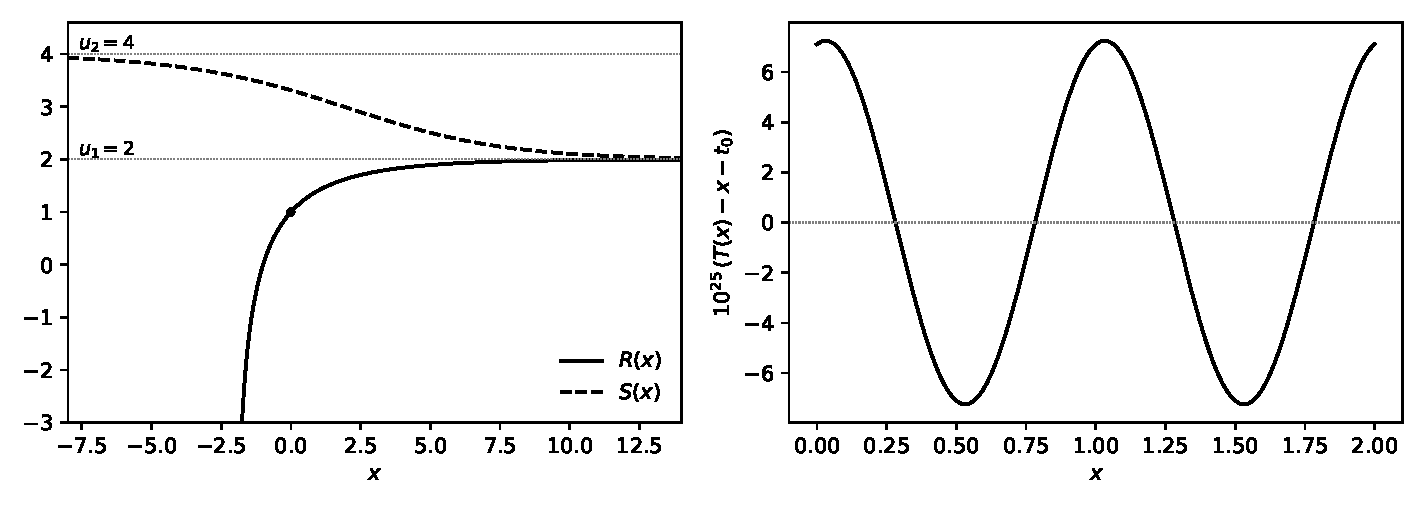
\includegraphics[width=\textwidth]{figures/fig2_regular.pdf}
  \caption{$b=\sqrt2$。左：$R(x)$（实线，$x>-2$）与 $S(x)$（虚线），点为 $R(0)=1$，点线为不动点 $2$、$4$。
  右：转移映射的非常数部分 $10^{25}(T(x)-x-t_0)$，它是实值、1-周期的，振幅 $2|t_1|=7.25\times10^{-25}$（\cref{ch2:ex:sqrt2-transition}）。
  脚本 \texttt{figures/fig2\_regular.py}。}
  \label{ch2:fig:regular}
\end{figure}

% ==================================================================
\section{两个分数次迭代}\label{ch2:sec:two}

由 \cref{prop:regular-periodic}(b)(c)，函数 $x\mapsto R(x+\ii h/2)$ 与 $x\mapsto S(x)$ 都是 $\R$ 到区间 $I=(u_1,u_2)$ 的实解析递减双射，都满足 $F(x+1)=f(F(x))$。
它们是 $f|_I$ 的两个实超函数：一个在 $u_1$ 处正则，一个在 $u_2$ 处正则。

\begin{proposition}\label{ch2:prop:two-abel}
设 $f$ 满足 \textup{(K1)--(K3)}。在 $I=(u_1,u_2)$ 上令
\[
  A_R(u):=R^{-1}(u)-\ii\frac h2=\frac{\log\bigl(\sigma(u)/|\sigma(\ustar)|\bigr)}{\log\lambda_1},\qquad
  A_S(u):=S^{-1}(u)=\frac{\log\bigl(-\sigma_{\mathrm{rep}}(u)\bigr)}{\log\lambda_2}.
\]
\begin{enumerate}[label=(\alph*)]
\item $A_R$ 与 $A_S$ 都是 $f|_I$ 的 Abel 函数，都是 $I$ 到 $\R$ 的实解析递减双射。
\item 存在实解析的 1-周期函数 $\theta$ 使 $A_R=A_S+\theta\circ A_S$。若令 $T(x):=R^{-1}(S(x))$（取 $\Ima T=h/2$ 的分支），则
  \[
    \theta(x)=T(x)-x-\ii\frac h2,\qquad T(x+1)=T(x)+1 .
  \]
\item 两个分数次迭代
  \[
    f_R^{\circ t}:=A_R^{-1}\circ(A_R+t)=\sigma^{-1}\circ(\lambda_1^{\,t}\sigma),\qquad
    f_S^{\circ t}:=A_S^{-1}\circ(A_S+t)=\sigma_{\mathrm{rep}}^{-1}\circ(\lambda_2^{\,t}\sigma_{\mathrm{rep}})
  \]
  （$\sigma^{-1}$、$\sigma_{\mathrm{rep}}^{-1}$ 指 $\sigma|_I$、$\sigma_{\mathrm{rep}}|_I$ 的反函数）
  对一切 $t$ 相同，当且仅当 $T-\id$ 是常数，即 $T$ 的 Fourier 系数 $t_n$（$n\ne0$）全为零。
\end{enumerate}
\end{proposition}

\begin{proof}
(a) 由 \cref{prop:regular-periodic}(e)。Abel 方程：$\sigma(f(u))=\lambda_1\sigma(u)$ 推出 $A_R(f(u))=A_R(u)+1$；$A_S$ 同理。
(b) 令 $\theta:=A_R\circ A_S^{-1}-\id=A_R\circ S-\id$，它是实解析函数的复合。由 $S(x+1)=f(S(x))$ 和 $A_R\circ f=A_R+1$，
$\theta(x+1)=A_R(f(S(x)))-x-1=A_R(S(x))-x=\theta(x)$。于是 $A_R=(\id+\theta)\circ A_S=A_S+\theta\circ A_S$。
$A_R(S(x))=R^{-1}(S(x))-\ii h/2=T(x)-\ii h/2$。$T(x+1)=T(x)+1$ 等价于 $\theta$ 的周期性。
(c) 两个表达式是 Abel 坐标定义的直接改写（$A_R+t$ 对应于 $\sigma$ 乘以 $\lambda_1^{\,t}$）。
记 $\varphi=\id+\theta$，它是 $\R$ 上的递增双射，$f_R^{\circ t}=A_S^{-1}\circ\varphi^{-1}\circ(\varphi\circ A_S+t)$。
所以 $f_R^{\circ t}=f_S^{\circ t}$ 对一切 $t$ 成立，当且仅当 $\varphi(y+t)=\varphi(y)+t$ 对一切 $y,t$ 成立，即 $\theta$ 为常数（第~\ref{ch:intro}~章的不唯一性命题）。
由 (b)，这等价于 $T-\id$ 为常数。
\end{proof}

$T$ 在实轴附近的带形上全纯，$T(z)-z=\sum_{n\in\Z}t_n\ee^{2\pi\ii nz}$；由 $\theta$ 取实值，$t_{-n}=\overline{t_n}$，$\Ima t_0=h/2$。
这是第~\ref{ch:transition}~章 \cref{def:transition} 的转移映射和 \cref{lem:realT} 的实结构。
「$R$ 和 $S$ 是两个不同的分数次迭代」的精确含义是：$T$ 不是平移。
对 Möbius 变换，$T$ 恰好是平移（\cref{ch2:ex:mobius}）；对 $b^w$，$T$ 不是平移，但差别极小：

\begin{example}[$b=\sqrt2$ 的转移映射]\label{ch2:ex:sqrt2-transition}
\texttt{figures/ch02\_sqrt2.py} 在 $16$ 个等距点上计算 $T(x)=R^{-1}(S(x))$，用离散 Fourier 变换求系数（混叠误差来自 $t_{\pm15}$，可以忽略）。结果（数值）：
\[
\begin{aligned}
  t_0&=-5.2840469112759295096+8.5715740896774235521\,\ii,\qquad \Ima t_0=h/2,\\
  t_1&=\overline{t_{-1}}=3.55397489161\times10^{-25}-7.19565846479\times10^{-26}\,\ii,\\
  |t_1|&=3.62608777302\times10^{-25},\qquad |t_2|=2.06254669064\times10^{-49}.
\end{aligned}
\]
因为 $|\ee^{-2\pi\ii t_0}|=\ee^{2\pi\Ima t_0}=\ee^{\pi h}$，$t_n$ 天然地含有因子 $\ee^{-n\pi h}=\Lam^{n/2}$（$\ee^{-\pi h}=4.0766\times10^{-24}$）。
去掉这个因子，得到第~\ref{ch:transition}~章的规范化系数 $\tau_n=t_n\ee^{-2\pi\ii nt_0}$：
\[
\begin{gathered}
  \tau_1=-0.00125909725971+0.0889407535848\,\ii,\\
  |\tau_1|=0.0889496653965,\qquad|\tau_2|=0.01241125793 .
\end{gathered}
\]
两个半迭代在 $u=3$ 处的值是
\[
\begin{aligned}
  f_R^{\circ1/2}(3)&=2.913786734633452607979441747\ldots,\\
  f_S^{\circ1/2}(3)&=2.913786734633452607979441917\ldots,
\end{aligned}
\]
相差 $-1.694\times10^{-25}$。它们在双精度下无法区分，但不相等。
\end{example}

这个例子预告了后面各章的三个结论。
\begin{enumerate}[label=(\arabic*)]
\item \emph{汇流。}第~\ref{ch:confluence}~章证明 $b\to\eta^-$ 时 $\tau_n\to B_n\ee^{2\pi\ii na}$（\cref{thm:confluence}），
  其中 $B_n$ 是抛物芽 $\ee^u-1$ 的逆 horn 映射的系数（\cref{def:horn}），$|B_1|=0.0890584364\ldots$，$|B_2|=0.0124873841\ldots$~\cite[\S2.1]{KneserPaper}。
  $b=\sqrt2$ 离 $\eta=1.44467$ 并不很近，$|\tau_1|$ 与 $|B_1|$ 已相差约 $0.12\%$，$|\tau_2|$ 与 $|B_2|$ 相差约 $0.6\%$。
  相位也接近：$\arg\tau_1=1.584952\ldots$，而极限相位是 $\arg B_1+2\pi a\equiv1.58653\ldots$（模 $2\pi$，\cite[\S2.1]{KneserPaper}）。
\item \emph{尺度。}$t_1$ 的大小 $\approx\ee^{-\pi h}|\tau_1|$ 是指数小的。第~\ref{ch:unfolding}~章证明 $h\sim\pi/\sqrt{a_2\gamma s}$（\cref{prop:scales}），所以这种指数小在鞍结附近是「超越所有阶」的。
\item \emph{缝合。}第~\ref{ch:sewing}~章的缝合解 $\Ksew=R\circ(\id+\sum_{n\ge0}c_n\ee^{2\pi\ii nz})$ 满足 $c_n=\Lam^n\bigl(\tau_n+O(\Lam)\bigr)$（\cref{thm:sewing}，$s$ 充分小时）。
  在 $z=\frac12$ 处，一阶近似给出
  \[
    \Ima\Ksew_{\sqrt2}(\tfrac12)\approx\Ima\bigl(c_1R'(\tfrac12)(\ee^{\ii\pi}-1)\bigr)=-2R'(\tfrac12)\,\Ima(\Lam\tau_1)=-1.18899697185\times10^{-48},
  \]
  其中 $R'(\frac12)=0.40221842463187347989$（同一脚本）。这与 \cite{KneserPaper} 用缝合方程直接算出的 $-1.18899697185\times10^{-48}$ 在所列的 $12$ 位上一致，
  也与 Paulsen 的 $-1.18899697\times10^{-48}$~\cite[\S6]{Paulsen2019} 在所给的 9 位上一致（第~\ref{ch:intro}~章）。
  若 \cref{thm:sewing} 的估计在 $b=\sqrt2$ 处适用，被忽略的项相对大小是 $O(\Lam)\approx10^{-47}$；
  但定理只对充分接近 $\eta$ 的 $b$ 证明，所以这里的一致是数值事实。
\end{enumerate}

% ==================================================================
\notes

\paragraph{Koenigs 定理。}
\cref{thm:koenigs} 属于 G.~Koenigs~\cite{Koenigs1884}。Schröder~\cite{Schroder1870} 在 1870 年研究了 \eqref{ch2:eq:schroder}；形式解（\cref{ch2:lem:formal}）的递推是标准的。
本章的证明（极限 \eqref{ch2:eq:koenigs-limit} 与直接的唯一性论证）沿用~\cite[\S8]{Milnor2006}；另见~\cite[Ch.~II]{CarlesonGamelin1993}。
Poincaré 函数（\cref{ch2:prop:poincare}）以 H.~Poincaré 命名。
关于中性不动点的线性化（Siegel、Brjuno、Cremer）见~\cite[\S11]{Milnor2006}，本书不需要。

\paragraph{正则解与 tetration。}
吸引不动点处的正则迭代是函数方程文献中的标准构造；对 tetration，它就是 $1<b<\eta$ 时通常所说的「正则 tetration」。
Kouznetsov 与 Trappmann~\cite{KouznetsovTrappmann2010} 研究了底数 $\sqrt2$ 的正则超指数，包括在两个不动点 $2$、$4$ 处构造的超指数及其复平面上的图像；
\cref{ch2:ex:four} 的四个实函数可以与之对照。
$S$ 与 $R^{-1}$ 的定义、$\sigma(\ustar)<0$ 的作用以及 \cref{prop:regular-periodic}(e) 的实结构取自~\cite[\S3.1]{KneserPaper}，
那里写的是 tetration（$w_0=1$）；一般开折的改写（用 (H4) 代替 $1<\ee^{\lambda_1}$）见 \texttt{sec-general.tex}。
\cref{ch2:lem:param} 是~\cite[Lemma~2.1]{KneserPaper}。
\cref{ch2:prop:regular-unique} 是第~\ref{ch:intro}~章的不唯一性命题与 Liouville 定理的直接结合；在~\cite{KneserPaper} 中没有单独陈述。

\paragraph{与后面各章的对应。}
本章对固定的 $f$ 讨论问题。第~\ref{ch:unfolding}~章让 $f=f_s$ 依赖参数 $s$，此时 $\lambda_1,\lambda_2\to1$，$h,h_2\to\infty$，$\Lam\to0$；
本章 (K1)--(K3) 由 (H1)--(H4) 对充分小的 $s>0$ 推出。
\cref{ch2:sec:two} 的 $T$ 在第~\ref{ch:transition}~章正式定义（\cref{def:transition}），并且那里把它延拓到实轴下方的一个带形，那是缝合与汇流发生的地方。

% ==================================================================
\exercises

\begin{exercise}\label{ch2:ex:series}
设 $f(z)=\lambda z+z^2$，$0<|\lambda|<1$。用 \eqref{ch2:eq:recursion} 证明 Koenigs 坐标的前几项是
\[
  \sigma(z)=z+\frac{z^2}{\lambda-\lambda^2}+\frac{2\,z^3}{(\lambda-\lambda^2)(1-\lambda^2)}+O(z^4).
\]
分母中出现的 $\lambda-\lambda^k$ 在 $\lambda\to1$ 时趋于零，这预示了抛物情形的困难。
\end{exercise}

\begin{exercise}\label{ch2:ex:eigen}
在 \cref{thm:koenigs} 的条件下，设 $\varphi$ 在 $p$ 附近全纯、不是常数，$\varphi(p)=0$，且 $\varphi\circ f=\mu\varphi$（$\mu\in\C$）。
证明存在正整数 $m$ 和常数 $c\ne0$，使 $\mu=\lambda^m$，$\varphi=c\,\sigma^m$。
\end{exercise}
\begin{hint}
在坐标 $\zeta=\sigma(u)$ 中考虑 $k=\varphi\circ\sigma^{-1}$，它满足 $k(\lambda\zeta)=\mu k(\zeta)$。比较幂级数的各项系数。
\end{hint}

\begin{exercise}\label{ch2:ex:real-branch}
设 $f$ 在实轴上取实值，$p\in\R$ 是吸引不动点，乘子 $0<\lambda<1$。对 $\ell=\log\lambda+2\pi\ii k$（$k\in\Z$）定义 $f^{\circ t}_{(\ell)}=\Psi\circ(\ee^{\ell t}\sigma)$。
证明：对固定的实数 $t$，$f_{(\ell)}^{\circ t}$ 在 $p$ 附近的实轴上取实值，当且仅当 $2kt\in\Z$；所以它对每个实数 $t$ 都取实值，当且仅当 $k=0$。
对 $t=\frac12$ 与奇数 $k$，$f_{(\ell)}^{\circ1/2}=\Psi\circ(-\sqrt\lambda\,\sigma)$ 是实的，它在 $p$ 附近递增还是递减？
\end{exercise}

\begin{exercise}\label{ch2:ex:mobius}
设 $f(u)=u/(2-u)$。它在 $u_1=0$、$u_2=1$ 处有不动点，乘子 $\frac12$ 和 $2$，并且在 $[\ustar,1]$（$\ustar=-\frac12$）上满足 (K3)。$f$ 不是整函数，但 \cref{def:regular-solution} 的公式仍有意义。
\begin{enumerate}[label=(\alph*)]
\item 证明 $\sigma(u)=u/(1-u)$，$\sigma_{\mathrm{rep}}(u)=-(1-u)/u$。
\item 写出 $R$、$S$，并证明 $T=R^{-1}\circ S$ 是平移 $T(z)=z+t_0$。求 $t_0$，并验证 $\Ima t_0=h/2$。
\item 由 \cref{ch2:prop:two-abel}(c) 说明：对这个 $f$，两个正则分数迭代在 $(0,1)$ 上相同。
\end{enumerate}
\end{exercise}
\begin{hint}
$y=u/(1-u)$ 把 $f$ 共轭成 $y\mapsto y/2$，$1/y$ 把 $f$ 共轭成 $y\mapsto 2y$。
\end{hint}

\begin{exercise}\label{ch2:ex:real-lines}
设 $f$ 满足 (K1)--(K3)。证明：对实数 $y$，$R(x+\ii y)$ 对一切充分大的实数 $x$ 取实值，当且仅当 $y\in\frac h2\Z$。
\end{exercise}

\begin{exercise}\label{ch2:ex:bw-domain}
对 $f(w)=b^w$（$1<b<\eta$，$w_0=1$）补全 \cref{ch2:ex:bw-singular} 的细节：证明 $R'(x)>0$ 于 $(-2,\infty)$，$R(-1)=0$，并利用 $R(x)=\log_bR(x+1)$ 证明 $x\downarrow-2$ 时 $R(x)\to-\infty$。
\end{exercise}

\begin{exercise}\label{ch2:ex:four}
对 $f(w)=b^w$（$1<b<\eta$），证明 $x\mapsto S(x+\ii h_2/2)$ 是实值的，严格递增，把 $\R$ 双射到 $(\ee^{\lambda_2},+\infty)$，并满足 $F(x+1)=b^{F(x)}$。
于是得到 $f$ 的四个实超函数：$R$（取值于 $(-\infty,\ee^{\lambda_1})$）、$R(\cdot+\ii h/2)$ 与 $S$（取值于 $(\ee^{\lambda_1},\ee^{\lambda_2})$）、$S(\cdot+\ii h_2/2)$（取值于 $(\ee^{\lambda_2},\infty)$）。
\end{exercise}
\begin{hint}
$-\lambda_2^{\,x+\ii h_2/2}=\lambda_2^{\,x}>0$。证明 $\Psi_2$ 把 $(0,\infty)$ 递增地映到 $(\ee^{\lambda_2},\infty)$：在 $0$ 附近 $\Psi_2'(0)=1>0$，
再用 $\Psi_2(\lambda_2y)=b^{\Psi_2(y)}$ 和 $b^w>w$（$w>\ee^{\lambda_2}$）。
\end{hint}

\begin{exercise}\label{ch2:ex:h2-h}
对 $f(w)=b^w$，令 $\lambda_1=1-\varepsilon$。
\begin{enumerate}[label=(\alph*)]
\item 由 $\lambda_1\ee^{-\lambda_1}=\lambda_2\ee^{-\lambda_2}$ 证明 $\lambda_2=1+\varepsilon+\frac23\varepsilon^2+O(\varepsilon^3)$。
\item 证明 $\frac1{\log\lambda_1}+\frac1{\log\lambda_2}=\frac13+O(\varepsilon)$，从而 $h_2-h\to\frac{2\pi}3$（$b\to\eta^-$）。
\item 用表~\ref{ch2:tab:sqrt2} 检验：$b=\sqrt2$ 时 $h_2-h=2.0930$，$2\pi/3=2.0944$。
\end{enumerate}
\end{exercise}
\begin{hint}
(a) 令 $\lambda_2=1+\delta$，比较 $(1-\varepsilon)\ee^{\varepsilon}=1-\frac{\varepsilon^2}2-\frac{\varepsilon^3}3+O(\varepsilon^4)$ 与 $(1+\delta)\ee^{-\delta}=1-\frac{\delta^2}2+\frac{\delta^3}3+O(\delta^4)$。
(b) $\frac1{\log(1-\varepsilon)}=-\frac1\varepsilon+\frac12+O(\varepsilon)$，$\frac1{\log\lambda_2}=\frac1\varepsilon-\frac16+O(\varepsilon)$。
一般开折的对应结论是 $h_2-h\to2\pi\rho$（\cref{prop:scales}）。
\end{hint}

\begin{exercise}\label{ch2:ex:complex-unique}
（较难）设 $p$ 是吸引不动点，乘子 $\lambda$ 是非实复数，$0<|\lambda|<1$。设 $F$ 在右半平面上全纯，$F(z+1)=f(F(z))$，且 $F(z)\to p$ 关于 $\Ima z$ 一致（$\Rea z\to+\infty$）。
证明 $F\equiv p$ 或存在 $\lambda$ 的一个对数 $\ell$ 和常数 $c\ne0$ 使 $F(z)=\Psi(c\,\ee^{\ell z})$。对数 $\ell$ 的哪些选取能出现？
\end{exercise}
\begin{hint}
固定一个对数 $\ell_0$，令 $\phi=\sigma(F)\ee^{-\ell_0z}$。它是 1-周期的，在带形上满足 $|\phi(x+\ii y)|\le C\ee^{|\Ima\ell_0||y|}$。
Fourier 系数 $\phi_n=\int_0^1\phi(x+\ii y)\ee^{-2\pi\ii n(x+\ii y)}\dd x$ 对每个 $y$ 都成立，令 $y\to\pm\infty$ 估计哪些 $\phi_n$ 可以非零。
再说明若有两个非零系数，$\sigma(F)$ 在某个方向上不趋于 $0$。
\end{hint}

\begin{exercise}\label{ch2:ex:T-monotone}
（较难，预告 \cref{lem:realT}）设 $f$ 满足 (K1)--(K3)，$T(x)=R^{-1}(S(x))$ 取 $\Ima T=h/2$ 的分支。证明 $T'(x)>0$ 对一切实数 $x$ 成立，
并说明为什么这推出 $T$ 在包含实轴的某个水平带内是单射。
\end{exercise}
\begin{hint}
$T'(x)=\dfrac{\sigma'(S(x))\,S'(x)}{\sigma(S(x))\log\lambda_1}$，逐个确定四个因子的符号。单射性：$T(x+1)=T(x)+1$，用紧性论证。
\end{hint}

\begin{exercise}\label{ch2:ex:numerics}
（数值）修改 \texttt{figures/ch02\_sqrt2.py}，对 $b=1.3,\ 1.4,\ 1.44$ 计算 $h$、$|t_1|$ 与 $|\tau_1|$，并与 $|B_1|=0.0890584364\ldots$ 比较。
说明为什么迭代步数 $N$ 必须随 $1/|\log\lambda_1|$ 增长，以及为什么工作精度必须超过 $\pi h/\log10$ 位才能看到 $t_1$。
\end{exercise}

% 第 3 章：抛物不动点：Fatou 坐标与 horn 映射
% 本章新增宏（\providecommand，见汇报）
\providecommand{\Patt}{P_{\mathrm{att}}}
\providecommand{\Prep}{P_{\mathrm{rep}}}
\providecommand{\Oatt}{\Omega_{\mathrm{att}}}
\providecommand{\Orep}{\Omega_{\mathrm{rep}}}
\providecommand{\lrep}{\ell_{\mathrm{rep}}}
\providecommand{\Arg}{\operatorname{Arg}}

\chapter{抛物不动点：Fatou 坐标与 horn 映射}\label{ch:fatou}

第~\ref{ch:koenigs}~章处理了双曲不动点：在乘子满足 $0<|\lambda|\ne1$ 的不动点附近，Koenigs 坐标把映射线性化，
取对数后得到 Abel 方程 $\Phi\circ f=\Phi+1$ 的解。当两个实不动点在鞍结中合并时，
乘子趋于 $1$，Koenigs 坐标退化。本章研究极限情形本身：一个乘子为 $1$ 的不动点，
即\textbf{抛物不动点}（parabolic fixed point）。

在抛物点附近，Abel 方程仍然有解，但解不再在整个邻域上存在，而是分别存在于两片
\textbf{花瓣}（petal）上：吸引花瓣上的 $\Phiatt$ 和排斥花瓣上的 $\Phirep$。两片花瓣
在不动点的上方和下方各有一个公共区域。在公共区域里比较两个坐标，得到一个与平移
$z\mapsto z+1$ 交换的映射，即 \textbf{horn 映射}（horn map）。它的 Fourier 系数 $B_n$
是芽在解析共轭下的不变量，也是本书后半部分的核心数据：第 7 章将证明，鞍结开折
在双曲一侧的转移映射不变量 $\tau_n$ 收敛到 $B_n\ee^{2\pi\ii na}$。

本章对一般的二重抛物芽 $g(u)=u+a_2u^2+a_3u^3+\cdots$（$a_2>0$）展开全部论证，
不使用指数函数的任何特殊性质。

\begin{goals}
\item 在坐标 $\zeta=-1/(a_2u)$ 中，$g$ 近似于平移 $\zeta\mapsto\zeta+1$；由此证明二重情形的 Leau--Fatou 花瓣定理，以及轨道渐近 $g^n(u)\approx-1/(a_2n)$。
\item 形式 Abel 函数 $\alpha(u)=-1/(a_2u)+\rho\log(-u)+\sum d_ku^k$ 存在且在相差常数的意义下唯一；迭代留数 $\rho=1-a_3/a_2^2$ 是形式共轭不变量。
\item Fatou 坐标 $\Phiatt$、$\Phirep$ 存在、单叶，并且用 $\alpha$ 归一化之后唯一。
\item 逆 horn 映射 $\horn^{-1}=\Phiatt\circ\Phirep^{-1}=z+\sum_{n\ge1}B_n\ee^{2\pi\ii nz}$ 没有常数项；逆下 horn 映射的常数项是 $2\pi\ii\rho$；乘积 $B_n\ee^{2\pi\ii na}$ 不依赖坐标的选取。
\item 当直接吸引域只含一个奇异值时 $B_1\ne0$；两个算例 $\ee^u-1$ 与 $u+u^2$ 的数值。
\end{goals}

%======================================================================
\section{二重抛物芽与坐标 \texorpdfstring{$\zeta$}{zeta}}\label{ch3:sec:germ}

\begin{definition}[二重抛物芽]\label{ch3:def:germ}
设 $g$ 在圆盘 $D_r=\{|u|<r\}$ 上全纯且单叶，
\[
 g(u)=u+a_2u^2+a_3u^3+O(u^4),\qquad a_2>0 .
\]
称 $g$ 是一个\textbf{二重抛物芽}（parabolic germ of multiplicity two），称
\[
 \rho:=1-\frac{a_3}{a_2^2}
\]
为它的\textbf{迭代留数}（iterative residue，法文 résidu itératif）。若 $g$ 的 Taylor
系数都是实数，称 $g$ 为\textbf{实芽}。
\end{definition}

条件 $a_2\ne0$ 说明 $0$ 是 $g(u)-u$ 的二重零点，即 $0$ 作为不动点的重数为 $2$。
若 $a_2\ne0$ 是任意复数，用 $u\mapsto cu$ 把它变成正数即可；本书的芽来自实鞍结开折
（第~\ref{ch:unfolding}~章），其中 $a_2>0$ 是自然的正规化。我们保留 $a_2$ 而不把它缩放为
$1$，因为第 4--9 章的公式要用到它。

逆映射 $g^{-1}$ 在 $0$ 的某个邻域上有定义，并且
\begin{equation}\label{ch3:eq:ginv}
 g^{-1}(u)=u-a_2u^2+(2a_2^2-a_3)u^3+O(u^4).
\end{equation}
（把 $u=v-a_2v^2+bv^3$ 代入 $g$ 并比较 $v^3$ 的系数，得 $b=2a_2^2-a_3$。）

\begin{lemma}[坐标 $\zeta$]\label{ch3:lem:zeta}
令 $\zeta=-1/(a_2u)$，并记
\[
 G(\zeta):=-\frac{1}{a_2\,g\bigl(-1/(a_2\zeta)\bigr)} .
\]
存在 $R_1>0$ 与 $C_1>0$，使得 $G$ 和 $G^{-1}$ 在 $\{|\zeta|>R_1\}$ 上全纯、单叶，并且
\begin{equation}\label{ch3:eq:G}
 \Bigl|G(\zeta)-\zeta-1-\frac{\rho}{\zeta}\Bigr|\le\frac{C_1}{|\zeta|^2},\qquad
 \Bigl|G^{-1}(\zeta)-\zeta+1+\frac{\rho}{\zeta}\Bigr|\le\frac{C_1}{|\zeta|^2}
 \qquad(|\zeta|>R_1).
\end{equation}
\end{lemma}

\begin{proof}
缩小 $r$，可设 $g(u)=u\bigl(1+x(u)\bigr)$，$x(u)=a_2u+a_3u^2+u^3k(u)$，其中 $k$ 在
$D_r$ 上有界，且 $|x(u)|\le1/2$。于是
$G(\zeta)=\zeta/(1+x)$，而
$\frac{1}{1+x}=1-x+x^2-\frac{x^3}{1+x}$。由 $a_2u=-1/\zeta$，
\[
 x=-\frac1\zeta+\frac{a_3}{a_2^2\zeta^2}+O(|\zeta|^{-3}),\qquad
 \frac1{1+x}=1+\frac1\zeta+\frac{1}{\zeta^2}-\frac{a_3}{a_2^2\zeta^2}+O(|\zeta|^{-3}).
\]
乘以 $\zeta$ 得 $G(\zeta)=\zeta+1+\rho/\zeta+O(|\zeta|^{-2})$，其中 $O$ 的常数只依赖于
$a_2$、$a_3$ 和 $\sup|k|$。对 $g^{-1}$ 用 \eqref{ch3:eq:ginv} 作同样的计算：此时
$x=1/\zeta+(2a_2^2-a_3)/(a_2^2\zeta^2)+O(|\zeta|^{-3})$，
$\zeta/(1+x)=\zeta-1+(1-2+a_3/a_2^2)/\zeta+O(|\zeta|^{-2})=\zeta-1-\rho/\zeta+O(|\zeta|^{-2})$。
单叶性来自 $g$、$g^{-1}$ 的单叶性和 $u\mapsto\zeta$ 是 Möbius 变换。
\end{proof}

由 \eqref{ch3:eq:G}，存在 $C_2$ 使 $|G(\zeta)-\zeta-1|\le C_2/|\zeta|$，
$|G^{-1}(\zeta)-\zeta+1|\le C_2/|\zeta|$。固定 $R_*\ge\sqrt2\max(R_1,\,4C_2,\,10)$。
于是当 $|\zeta|\ge R_*/\sqrt2$ 时
\begin{equation}\label{ch3:eq:quarter}
 |G(\zeta)-\zeta-1|\le\tfrac14,\qquad |G^{-1}(\zeta)-\zeta+1|\le\tfrac14,\qquad
 \Bigl|\frac{G(\zeta)}{\zeta}-1\Bigr|\le\frac{5}{4|\zeta|}\le\frac{1}{5}.
\end{equation}

\begin{example}\label{ch3:ex:zeta}
(1) $g(u)=u+u^2$：$a_2=1$，$a_3=0$，$\rho=1$。此时 $G$ 可以精确算出：
$G(\zeta)=-1/(u(1+u))=\zeta^2/(\zeta-1)=\zeta+1+\frac{1}{\zeta-1}$。

(2) $g(u)=\ee^u-1=u+\tfrac12u^2+\tfrac16u^3+\cdots$：$a_2=\tfrac12$，$a_3=\tfrac16$，
$\rho=1-\tfrac{1/6}{1/4}=\tfrac13$，$\zeta=-2/u$，
$G(\zeta)=-2/(\ee^{-2/\zeta}-1)=\zeta+1+\frac{1}{3\zeta}+O(\zeta^{-3})$
（展开 $x/(\ee^x-1)$ 的 Bernoulli 级数可知 $\zeta^{-2}$ 项为零）。这是 tetration 在
$b=\eta=\ee^{1/\ee}$ 处的芽：在 $w=\ee(1+u)$ 中，$w\mapsto\eta^w$ 变成 $u\mapsto\ee^u-1$
（\cite[\S2.1]{KneserPaper}）。

(3) $g(u)=u/(1-u)=u+u^2+u^3+\cdots$：$\rho=0$，且 $G(\zeta)=\zeta+1$ 恰为平移。
\end{example}

%======================================================================
\section{Leau--Fatou 花瓣}\label{ch3:sec:petals}

记
\[
 s(\zeta):=\Rea\zeta+|\Ima\zeta|,\qquad t(\zeta):=-\Rea\zeta+|\Ima\zeta| .
\]

\begin{definition}[花瓣]\label{ch3:def:petals}
对 $R\ge R_*$，令
\[
 \Oatt(R)=\{\zeta:\ s(\zeta)>R\},\qquad \Orep(R)=\{\zeta:\ t(\zeta)>R\},
\]
并称它们在 $u$ 平面中的原像
$\Patt(R)=\{u\ne0:\ -1/(a_2u)\in\Oatt(R)\}$、
$\Prep(R)=\{u\ne0:\ -1/(a_2u)\in\Orep(R)\}$
为\textbf{吸引花瓣}与\textbf{排斥花瓣}（attracting / repelling petal）。
\end{definition}

$\Oatt(R)$ 是平面去掉一个顶点在 $R$、开口向左、张角 $\pi/2$ 的闭角形区域；
$\Orep(R)=-\Oatt(R)$。$\Oatt(R)$ 是两个半平面 $\{\Rea\zeta\pm\Ima\zeta>R\}$ 之并，所以在 $u$ 平面中，
$\Patt(R)$ 是两个边界过原点的开圆盘之并，含有负实轴的一段，见\cref{ch3:fig:petals}(a)。下面几条初等事实反复使用：
\begin{enumerate}[label=(\alph*)]
\item $s(\zeta)\le|\Rea\zeta|+|\Ima\zeta|\le\sqrt2|\zeta|$，同样 $t(\zeta)\le\sqrt2|\zeta|$；
\item $\Oatt(R)\subset\{|\Arg\zeta|<3\pi/4\}$，$\Orep(R)\subset\{|\Arg(-\zeta)|<3\pi/4\}$，其中 $\Arg$ 是主值辐角；
\item $\Oatt(R)\cup\Orep(R)=\{|\Rea\zeta|+|\Ima\zeta|>R\}\supset\{|\zeta|>R\}$；
\item $\Oatt(R)\cap\Orep(R)=\{|\Ima\zeta|>R+|\Rea\zeta|\}$，它有两个连通分支 $W_+(R)\subset\{\Ima\zeta>0\}$、$W_-(R)\subset\{\Ima\zeta<0\}$。
\end{enumerate}
(b) 的理由：若 $\zeta\in\Oatt(R)$ 且 $\Rea\zeta<0$，则 $|\Ima\zeta|>R+|\Rea\zeta|>|\Rea\zeta|$。
(c) 的理由：$\max(s,t)=|\Rea\zeta|+|\Ima\zeta|$。注意 $\zeta$ 与 $u$ 的上下半平面一致：
$-1/u$ 把上半平面映为上半平面，所以 $\Ima\zeta>0\iff\Ima u>0$。

\begin{theorem}[Leau--Fatou 花瓣定理，二重情形]\label{ch3:thm:flower}
设 $g$ 是二重抛物芽，$R\ge R_*$。
\begin{enumerate}
\item $G(\Oatt(R))\subset\Oatt(R)$，且 $s(G(\zeta))\ge s(\zeta)+\tfrac12$；
 $G^{-1}(\Orep(R))\subset\Orep(R)$，且 $t(G^{-1}(\zeta))\ge t(\zeta)+\tfrac12$。
\item 对 $u\in\Patt(R)$ 和 $n\ge0$，$|g^n(u)|\le\sqrt2/\bigl(a_2(R+n/2)\bigr)$；特别地 $g^n\to0$ 在 $\Patt(R)$ 上一致成立。对 $\Prep(R)$ 与 $g^{-n}$ 有同样的结论。
\item $\Patt(R)\cup\Prep(R)\cup\{0\}\supset D_{1/(a_2R)}$。
\item 若 $u\ne0$，$g^n(u)\to0$ 且对所有 $n$ 有 $g^n(u)\ne0$，则 $n$ 充分大时 $g^n(u)\in\Patt(R)$。对后向轨道与 $\Prep(R)$ 有同样的结论。
\item 对 $u\in\Patt(R)$，$n\,g^n(u)\to-1/a_2$，且 $\Arg(-g^n(u))\to0$；收敛关于 $u$ 在 $\Patt(R)$ 的紧子集上一致。即轨道沿负实轴方向切向地趋于 $0$，并且 $g^n(u)\approx-1/(a_2n)$。
\end{enumerate}
\end{theorem}

\begin{proof}
(1) 若 $\zeta\in\Oatt(R)$，由 (a) 有 $|\zeta|\ge s(\zeta)/\sqrt2>R_*/\sqrt2$，于是
\eqref{ch3:eq:quarter} 给出 $\Rea G(\zeta)\ge\Rea\zeta+\tfrac34$，
$|\Ima G(\zeta)|\ge|\Ima\zeta|-\tfrac14$，相加得 $s(G(\zeta))\ge s(\zeta)+\tfrac12$。
排斥一侧同理。

(2) 由 (1)，$s(G^n\zeta)\ge R+n/2$，再由 (a)，$|G^n\zeta|\ge(R+n/2)/\sqrt2$，而
$|g^n(u)|=1/(a_2|G^n\zeta|)$。

(3) 由 (c)：$|u|<1/(a_2R)$ 等价于 $|\zeta|>R$。

(4) 记 $\zeta_n=-1/(a_2g^n(u))$，则 $\zeta_n\to\infty$，故对 $n\ge n_0$ 有 $|\zeta_n|>R$，从而
$\zeta_n\in\Oatt(R)\cup\Orep(R)$。若某个 $\zeta_n\in\Oatt(R)$，由 (1) 以后都在其中。
否则对所有 $n\ge n_0$，$\zeta_n\in\Orep(R)$，且 $\zeta_n=G^{-1}(\zeta_{n+1})$，由 (1)
$t(\zeta_n)\ge t(\zeta_{n+1})+\tfrac12$。于是 $t(\zeta_n)\le t(\zeta_{n_0})-(n-n_0)/2\to-\infty$，
与 $t(\zeta_n)>R$ 矛盾。后向轨道的论证对称。

(5) 记 $\zeta_k=G^k\zeta$。由 $|G(\zeta)-\zeta-1|\le C_2/|\zeta|$ 和 (2)，
\[
 |\zeta_n-\zeta-n|\le\sum_{k<n}\frac{C_2}{|\zeta_k|}
 \le\sqrt2C_2\sum_{k<n}\frac{1}{R+k/2}
 \le\sqrt2C_2\Bigl(\frac1R+2\log\Bigl(1+\frac{n}{2R}\Bigr)\Bigr).
\]
所以 $\zeta_n=n+O(\log n)$，$O$ 在 $\zeta$ 的有界集上一致。于是
$n\,g^n(u)=-n/(a_2\zeta_n)\to-1/a_2$；又 $\Rea\zeta_n\ge n/2$、$\Ima\zeta_n=O(\log n)$，故
$\Arg\zeta_n\to0$，而 $\Arg(-g^n(u))=-\Arg\zeta_n$。
\end{proof}

更精确的渐近式（含 $\log n/n^2$ 项）要用到 Fatou 坐标，见\cref{ch3:cor:orbit}。

\begin{definition}[抛物吸引域]\label{ch3:def:basin}
设 $g$ 是整函数 $f$ 在 $0$ 处的芽。称
$\mathfrak B=\{u\in\C:\ \text{存在 }n\ge0\text{ 使 }f^n(u)\in\Patt(R)\}$
为 $0$ 的\textbf{抛物吸引域}（parabolic basin），称 $\mathfrak B$ 中含 $\Patt(R)$ 的连通分支
$\mathcal A$ 为\textbf{直接吸引域}（immediate basin）。
\end{definition}

由\cref{ch3:thm:flower}(4)，$\mathfrak B$ 恰为满足 $f^n(u)\to0$ 且 $f^n(u)\ne0$ 的点集，
因此与 $R$ 无关；$\Patt(R)$ 连通，所以 $\mathcal A$ 也与 $R$ 无关。显然
$f^{-1}(\mathfrak B)=\mathfrak B$。

\begin{remark}[实芽的实吸引区间]\label{ch3:rem:real-basin}
设 $f$ 是实整函数，$\ustar<0$，且在 $[\ustar,0)$ 上 $f$ 递增并满足 $f(u)>u$。
则对 $u\in[\ustar,0)$，$u<f(u)<f(0)=0$，所以轨道严格递增且有上界 $0$，其极限是
$[\ustar,0]$ 中的不动点；$[\ustar,0)$ 中没有不动点，故极限为 $0$。因此
$[\ustar,0)\subset\mathcal A$。这正是第 4 章假设 (H4) 中基点所处的位置
（\cref{def:unfolding}）。对 $\ee^u-1$，整条负实轴都在 $\mathcal A$ 中。对 $u+u^2$，上述条件在 $[-\tfrac12,0)$ 上成立；
$f$ 把 $(-1,0)$ 映入 $[-\tfrac14,0)$，所以整个区间 $(-1,0)$ 在 $\mathcal A$ 中。
\end{remark}

%======================================================================
\section{形式 Abel 函数与迭代留数}\label{ch3:sec:formal}

我们要找 Abel 方程 $\alpha\circ g=\alpha+1$ 的形式解。由\cref{ch3:lem:zeta}，在 $\zeta$
坐标中 $G(\zeta)=\zeta+1+\rho/\zeta+O(\zeta^{-2})$。令 $\chi(\zeta)=\zeta-\rho\log\zeta$，则
$\chi(G(\zeta))=\zeta+1+\frac\rho\zeta-\rho\log\zeta-\rho\log\bigl(1+\frac1\zeta+O(\zeta^{-2})\bigr)=\chi(\zeta)+1+O(\zeta^{-2})$。这提示首项应为
$\zeta-\rho\log\zeta=-1/(a_2u)+\rho\log(-u)+\text{常数}$。

\textbf{形式框架。} 考虑形如
\begin{equation}\label{ch3:eq:class}
 \beta(u)=\frac{A}{u}+c\log(-u)+\varphi(u),\qquad A,c\in\C,\ \varphi\in\C[[u]]
\end{equation}
的形式表达式。对二重抛物芽 $g$（这里只用它的 Taylor 级数），定义
\[
 \beta\circ g-\beta:=A\Bigl(\frac1{g(u)}-\frac1u\Bigr)+c\,L_g(u)+\bigl(\varphi\circ g-\varphi\bigr),
 \qquad L_g(u):=\log\frac{g(u)}{u}\in u\C[[u]] ,
\]
其中 $L_g$ 是 $\log(1+a_2u+a_3u^2+\cdots)$ 的形式展开。因为
\begin{equation}\label{ch3:eq:inv-diff}
 \frac1{g}-\frac1u=\frac{u-g}{ug}=-\frac{a_2+a_3u+\cdots}{1+a_2u+\cdots}
 =-a_2+(a_2^2-a_3)u+O(u^2),
\end{equation}
$\beta\circ g-\beta$ 是 $\C[[u]]$ 中的元素。这一定义与收敛情形一致：若 $\log(-u)$
沿着从 $u$ 到 $g(u)$ 的短线段连续延拓，则 $\log(-g(u))-\log(-u)=\log(g(u)/u)$
（见\cref{ch3:lem:defect}）。

\begin{lemma}[差分算子]\label{ch3:lem:Delta}
记 $\Delta\varphi=\varphi\circ g-\varphi$。则对 $k\ge1$，
$\Delta(u^k)=ka_2u^{k+1}+O(u^{k+2})$，并且 $\Delta$ 是从 $u\C[[u]]$ 到 $u^2\C[[u]]$ 的线性
双射。$\Delta$ 在 $\C[[u]]$ 上的核是常数。
\end{lemma}

\begin{proof}
$g^k-u^k=u^k\bigl((1+a_2u+\cdots)^k-1\bigr)=ka_2u^{k+1}+O(u^{k+2})$。对
$\varphi=\sum_{k\ge1}\varphi_ku^k$，$\Delta\varphi$ 的 $u^{m+1}$ 项系数等于
$ma_2\varphi_m$ 加上只含 $\varphi_1,\dots,\varphi_{m-1}$ 的线性组合。这是对角元
$ma_2\ne0$ 的下三角无穷线性方程组，所以对任意右端 $\sum_{m\ge1}r_{m+1}u^{m+1}$ 可逐阶
唯一解出 $\varphi_1,\varphi_2,\dots$。常数显然在核中，而 $u\C[[u]]$ 中的核为零。
\end{proof}

\begin{theorem}[形式 Abel 函数]\label{ch3:thm:formal}
设 $g$ 是二重抛物芽。
\begin{enumerate}
\item 在形如 \eqref{ch3:eq:class} 的表达式中，满足 $\beta\circ g-\beta=1$ 的解必有
 $A=-1/a_2$、$c=\rho$。
\item 存在唯一的 $\varphi\in u\C[[u]]$（即无常数项），使
 $\alpha(u)=-\frac1{a_2u}+\rho\log(-u)+\varphi(u)$ 满足 $\alpha\circ g=\alpha+1$；
 \eqref{ch3:eq:class} 中的全部解是 $\alpha+\text{常数}$。
\item 若 $g$ 是实芽，则 $\varphi$ 的系数都是实数。
\end{enumerate}
\end{theorem}

\begin{definition}[形式 Abel 函数]\label{def:formal-abel}
\Cref{ch3:thm:formal}(2) 中的
\[
 \alpha(u)=-\frac{1}{a_2u}+\rho\log(-u)+\sum_{k\ge1}d_ku^k,\qquad \alpha\circ g=\alpha+1,
\]
称为 $g$ 的\textbf{形式 Abel 函数}（formal Abel function）；它的归一化是幂级数部分没有常数项。
记它的截断为
\[
 \alpha_N(u)=-\frac{1}{a_2u}+\rho\log(-u)+\sum_{k=1}^Nd_ku^k\qquad(N\ge0),
\]
特别地 $\alpha_0(u)=-1/(a_2u)+\rho\log(-u)$。$\log(-u)$ 取哪个分支，要等到它作为函数
使用时（\cref{ch3:sec:fatou}）才规定。
\end{definition}

\begin{proof}[\cref{ch3:thm:formal} 的证明]
(1) 由 \eqref{ch3:eq:inv-diff} 和 $L_g=a_2u+O(u^2)$，并由\cref{ch3:lem:Delta}
（$\Delta\varphi\in u^2\C[[u]]$），
\[
 \beta\circ g-\beta=-Aa_2+\bigl(A(a_2^2-a_3)+ca_2\bigr)u+O(u^2).
\]
令它等于 $1$：常数项给出 $A=-1/a_2$；$u$ 项给出
$c=-A(a_2^2-a_3)/a_2=1-a_3/a_2^2=\rho$。

(2) 取 $A=-1/a_2$、$c=\rho$，方程化为
$\Delta\varphi=r$，$r:=1+\frac{1}{a_2}\bigl(\frac1g-\frac1u\bigr)-\rho L_g$。由 (1) 的计算，
$r$ 的常数项和 $u$ 项都是零，即 $r\in u^2\C[[u]]$。由\cref{ch3:lem:Delta}，在 $u\C[[u]]$
中有唯一解；全部解相差 $\Delta$ 的核，即常数。

(3) 实芽时 $r$ 的系数是实数，三角方程组的解也是实数。
\end{proof}

逐阶求解给出系数的显式公式。例如（习题~\ref{ch3:exe:d1}）
\begin{equation}\label{ch3:eq:d1}
 d_1=\frac{2a_3^2+a_2^2a_3-2a_2a_4-a_2^4}{2a_2^3}.
\end{equation}

\begin{example}[两个形式 Abel 函数]\label{ch3:ex:formal}
用 \texttt{sympy} 逐阶求解（与 \texttt{docs/generality\_check.py} 中 \texttt{Alpha} 类的
浮点输出一致）：
\begin{align*}
 \ee^u-1:&\quad \alpha(u)=-\frac2u+\frac13\log(-u)-\frac{u}{36}+\frac{u^2}{540}+\frac{u^3}{7776}-\frac{71\,u^4}{435456}+\cdots,\\
 u+u^2:&\quad \alpha(u)=-\frac1u+\log(-u)-\frac{u}{2}+\frac{u^2}{3}-\frac{13\,u^3}{36}+\frac{113\,u^4}{240}+\cdots.
\end{align*}
第一行即论文的 \cite[\S2.1]{KneserPaper} 中的展开（论文记系数为 $c^\alpha_k$）。对
$g(u)=u/(1-u)$，$\alpha(u)=-1/u$ 精确成立。
\end{example}

\begin{proposition}[迭代留数是形式不变量]\label{ch3:prop:rho-invariant}
设 $h(v)=cv+O(v^2)\in\C[[v]]$，$c\ne0$，$\tilde g:=h^{-1}\circ g\circ h$（形式复合）。则
$\tilde g(v)=v+\tilde a_2v^2+\tilde a_3v^3+\cdots$，$\tilde a_2=ca_2$，并且
$\tilde\rho:=1-\tilde a_3/\tilde a_2^2=\rho$。
\end{proposition}

\begin{proof}
$\tilde a_2=ca_2$ 由比较 $v^2$ 系数得到。考虑 $\alpha\circ h$，其中
$\log(-h(v))$ 按 $\log(-v)+\log c+\log\bigl(h(v)/(cv)\bigr)$ 理解（$\log c$ 取定任一值）。
写 $h(v)=cv(1+e_1v+\cdots)$，则
\[
 \alpha(h(v))=-\frac{1}{a_2cv}(1-e_1v+\cdots)+\rho\log(-v)+\rho\log c+O(v)
 =-\frac{1}{\tilde a_2v}+\rho\log(-v)+\tilde\varphi(v),
\]
$\tilde\varphi\in\C[[v]]$。另一方面
$(\alpha\circ h)\circ\tilde g=\alpha\circ g\circ h=\alpha\circ h+1$，所以 $\alpha\circ h$ 是
$\tilde g$ 的、形如 \eqref{ch3:eq:class} 的 Abel 方程的解。由\cref{ch3:thm:formal}(1)，
其对数项系数等于 $\tilde\rho$。故 $\tilde\rho=\rho$。
\end{proof}

\begin{remark}[形式分类]\label{ch3:rem:formal-class}
\Cref{ch3:prop:rho-invariant} 的逆命题也成立：两个 $a_2$ 相同的二重抛物芽在形式上
通过切于恒等的变换共轭，当且仅当它们的迭代留数相同。一个标准代表是向量场
$X_{a_2,\rho}=\frac{a_2u^2}{1+\rho a_2u}\,\partial_u$ 的时间一映射；它的时间函数恰好是
$-1/(a_2u)+\rho\log(-u)$（习题~\ref{ch3:exe:normal-form}）。因此形式理论里只有
$(a_2,\rho)$ 两个不变量，而 $a_2$ 可以用缩放消去。下面将看到，解析分类需要无穷多个
额外的不变量，即 horn 映射。
\end{remark}

\begin{remark}[发散性]\label{ch3:rem:divergence}
级数 $\sum d_ku^k$ 一般是发散的。对 $\ee^u-1$ 和 $u+u^2$，这将由 $B_1\ne0$ 推出
（\cref{ch3:cor:divergence}）。Écalle 证明了它是 Borel 可和的，其 Stokes 现象恰好由
horn 映射描述 \cite{Ecalle1981,DudkoSauzin2014}；本书不用这一事实。
\end{remark}

%======================================================================
\section{Fatou 坐标}\label{ch3:sec:fatou}

\subsection{对数的分支与单步误差}
在吸引花瓣上，$\zeta\in\Oatt(R)\subset\{|\Arg\zeta|<3\pi/4\}$，而 $-u=1/(a_2\zeta)$，
所以 $|\Arg(-u)|<3\pi/4$。我们在 $\Patt(R)$ 上用主值 $\Log(-u)$。在排斥花瓣上
$|\Arg u|<3\pi/4$，我们用
\begin{equation}\label{ch3:eq:lrep}
 \lrep(u):=\Log u-\ii\pi\qquad(u\in\Prep(R)).
\end{equation}
它是 $\log(-u)$ 在 $\Prep(R)$ 上的一个连续分支，并且在上半平面与主值 $\Log(-u)$ 相同，
在下半平面等于 $\Log(-u)-2\pi\ii$。相应地记
\[
 \alpha_N^{\mathrm{att}}(u)=-\frac1{a_2u}+\rho\Log(-u)+\sum_{k=1}^Nd_ku^k,\qquad
 \alpha_N^{\mathrm{rep}}(u)=-\frac1{a_2u}+\rho\,\lrep(u)+\sum_{k=1}^Nd_ku^k .
\]
在 $\zeta$ 坐标中，$\alpha_0^{\mathrm{att}}=\zeta-\rho\Log\zeta-\rho\log a_2$
（因为 $a_2>0$ 且 $\zeta\notin(-\infty,0]$）。

\begin{lemma}[单步误差]\label{ch3:lem:defect}
缩小 $r$ 使 $|g(u)/u-1|<1/5$ 在 $D_r$ 上成立。对 $N\ge0$ 令
\[
 E_N(u):=\frac{1}{a_2u}-\frac{1}{a_2g(u)}+\rho\Log\frac{g(u)}{u}
 +\sum_{k=1}^Nd_k\bigl(g(u)^k-u^k\bigr)-1 .
\]
则 $E_N$ 在 $D_r$ 上全纯（$0$ 是可去奇点），并存在 $M_N$ 使
$|E_N(u)|\le M_N|u|^{N+2}$（$|u|\le r/2$）。若 $R$ 充分大，则对 $u\in\Patt(R)$ 有
$\alpha_N^{\mathrm{att}}(g(u))-\alpha_N^{\mathrm{att}}(u)-1=E_N(u)$；对 $u,g(u)\in\Prep(R)$ 有
$\alpha_N^{\mathrm{rep}}(g(u))-\alpha_N^{\mathrm{rep}}(u)-1=E_N(u)$。
\end{lemma}

\begin{proof}
由 \eqref{ch3:eq:inv-diff}，$1/u-1/g(u)$ 在 $0$ 处可去；$g(u)/u$ 在 $D_r$ 上取值于
$\{|w-1|<1/5\}$，其主值对数全纯。所以 $E_N$ 全纯，其 Taylor 级数等于形式表达式
$\alpha_N\circ g-\alpha_N-1$。由于 $\alpha\circ g-\alpha-1=0$，
\[
 \alpha_N\circ g-\alpha_N-1=-\Delta\Bigl(\sum_{k>N}d_ku^k\Bigr)\in u^{N+2}\C[[u]]
\]
（\cref{ch3:lem:Delta}）。故 $E_N(u)/u^{N+2}$ 在 $D_r$ 上全纯，在 $\overline{D_{r/2}}$ 上有界。

对分支：若 $u\in\Patt(R)$，则 $g(u)\in\Patt(R)$（\cref{ch3:thm:flower}(1)），
$\Arg(-u)$、$\Arg(-g(u))$ 都在 $(-3\pi/4,3\pi/4)$ 中，其差在 $(-3\pi/2,3\pi/2)$ 中，
且模 $2\pi$ 同余于 $\Arg(g(u)/u)$，而 $|\Arg(g(u)/u)|<\pi/4$。若二者不相等，差至少为
$2\pi-\pi/4>3\pi/2$，不可能。所以 $\Log(-g(u))-\Log(-u)=\Log(g(u)/u)$。排斥一侧把
$\Arg(-\cdot)$ 换成 $\Arg(\cdot)$，论证相同。
\end{proof}

\begin{lemma}[轨道求和]\label{ch3:lem:sum}
设 $R\ge R_*$，$m\ge2$。对 $u\in\Patt(R)$，$\zeta=-1/(a_2u)$，
\[
 \sum_{k\ge0}|g^k(u)|^m\le3\Bigl(\frac{\sqrt2}{a_2}\Bigr)^m s(\zeta)^{1-m}.
\]
对 $u\in\Prep(R)$，把 $g^k$ 换成 $g^{-k}$、$s$ 换成 $t$，结论相同。
\end{lemma}

\begin{proof}
由\cref{ch3:thm:flower}(1) 和 (a)，$|g^k(u)|\le\sqrt2/(a_2(s+k/2))$，$s=s(\zeta)\ge R_*\ge1$。而
$\sum_{k\ge0}(s+k/2)^{-m}\le s^{-m}+\int_0^\infty(s+x/2)^{-m}\dd x=s^{-m}+\frac{2s^{1-m}}{m-1}\le3s^{1-m}$。
\end{proof}

\subsection{存在性、唯一性与单叶性}

\begin{theorem}[Fatou 坐标]\label{thm:fatou-coordinates}
设 $g$ 是二重抛物芽，$\alpha$ 是它的形式 Abel 函数。存在 $R_0\ge R_*$，使对 $R\ge R_0$：
\begin{enumerate}
\item （存在）对每个 $N\ge0$，极限
 \[
  \Phiatt(u):=\lim_{n\to\infty}\bigl[\alpha_N^{\mathrm{att}}(g^n(u))-n\bigr]
 \]
 在 $\Patt(R)$ 上一致存在且与 $N$ 无关；$\Phiatt$ 在 $\Patt(R)$ 上全纯，
 $\Phiatt\circ g=\Phiatt+1$。
\item （渐近）存在常数 $K_N$，使
 $|\Phiatt(u)-\alpha_N^{\mathrm{att}}(u)|\le K_N\,s(\zeta)^{-N-1}$，$\zeta=-1/(a_2u)$。
 特别地，对每个 $\delta>0$，当 $u\to0$ 且 $|\Arg(-u)|\le3\pi/4-\delta$ 时，
 $\Phiatt(u)=\alpha_N^{\mathrm{att}}(u)+O(|u|^{N+1})$；即 $\Phiatt$ 以 $\alpha$ 为渐近展开。
\item （单叶）$\Phiatt$ 在 $\Patt(R)$ 上单叶；对每个 $w\in\C$，当 $n$ 充分大时
 $w+n\in\Phiatt(\Patt(R))$。
\item （唯一）若 $\Phi$ 在 $\Patt(R)$ 上全纯，$\Phi\circ g=\Phi+1$，且
 $\Phi-\alpha_0^{\mathrm{att}}$ 在 $\Patt(R)$ 上有界，则 $\Phi-\Phiatt$ 是常数；若再有
 某个 $u$ 使 $\Phi(g^nu)-\alpha_0^{\mathrm{att}}(g^nu)\to0$，则 $\Phi=\Phiatt$。
\item （排斥坐标）在 $\Prep(R)$ 上，
 $\Phirep(u):=\lim_{n\to\infty}\bigl[\alpha_N^{\mathrm{rep}}(g^{-n}(u))+n\bigr]$
 存在、全纯、单叶，满足 $\Phirep\circ g^{-1}=\Phirep-1$，
 $|\Phirep-\alpha_N^{\mathrm{rep}}|\le K_N\,t(\zeta)^{-N-1}$；对每个 $w$，$n$ 充分大时
 $w-n\in\Phirep(\Prep(R))$；唯一性与 (4) 相同（把 $\alpha_0^{\mathrm{att}}$ 换成
 $\alpha_0^{\mathrm{rep}}$，$g$ 换成 $g^{-1}$）。
\item （整体延拓）若 $g$ 是整函数 $f$ 的芽，则 $\Phiatt$ 延拓为抛物吸引域 $\mathfrak B$
 上的全纯函数，$\Phiatt\circ f=\Phiatt+1$；$\Phirep^{-1}$ 延拓为整函数 $\psi_{\mathrm{rep}}$，
 $\psi_{\mathrm{rep}}(z+1)=f(\psi_{\mathrm{rep}}(z))$。
\item （实芽）若 $g$ 是实芽，则 $\Patt(R)$、$\Prep(R)$ 关于实轴对称，并且
 \[
  \Phiatt(\bar u)=\overline{\Phiatt(u)},\qquad \Phirep(\bar u)=\overline{\Phirep(u)}-2\pi\ii\rho .
 \]
 特别地 $\Phiatt$ 在 $\Patt(R)\cap\R=(-1/(a_2R),0)$ 上取实值；若 $f$ 是实整函数，则 (6) 中的
 $\Phiatt$ 在 $\mathfrak B\cap\R$ 上取实值。
\end{enumerate}
称 $\Phiatt$、$\Phirep$ 为 $g$ 的\textbf{吸引、排斥 Fatou 坐标}（attracting / repelling Fatou
coordinates），称 $\psi_{\mathrm{rep}}$ 为\textbf{排斥参数化}（repelling parametrisation）。
\end{theorem}

归一化的含义是：两个 Fatou 坐标用\emph{同一个}形式 Abel 函数 $\alpha$ 归一化，
即 $\Phi-\alpha\to0$（在 (2) 的意义下）。$\alpha$ 的幂级数部分不含常数项；对数的分支在
吸引一侧取主值，在排斥一侧取 \eqref{ch3:eq:lrep}。这三项约定一起决定了 $B_n$。

\begin{proof}
以下 $\zeta=-1/(a_2u)$，并把 $\Patt(R)$ 上的函数也看成 $\Oatt(R)$ 上的函数。

\emph{(1)(2) 存在与渐近。} 对 $u\in\Patt(R)$，令 $u_k=g^k(u)\in\Patt(R)$。由\cref{ch3:lem:defect}，
\[
 \alpha_N^{\mathrm{att}}(u_n)-n=\alpha_N^{\mathrm{att}}(u)+\sum_{k=0}^{n-1}E_N(u_k).
\]
由\cref{ch3:lem:defect,ch3:lem:sum}（$m=N+2$；$R$ 大时 $\Patt(R)\subset D_{r/2}$），
$\sum_{k\ge0}|E_N(u_k)|\le K_Ns(\zeta)^{-N-1}$，$K_N=3M_N(\sqrt2/a_2)^{N+2}$。所以级数在
$\Patt(R)$ 上一致收敛，极限
$\Phiatt=\alpha_N^{\mathrm{att}}+\sum_{k\ge0}E_N\circ g^k$ 全纯，并满足 (2) 的第一个估计。
由于 $\alpha_N^{\mathrm{att}}-\alpha_{N'}^{\mathrm{att}}=O(u)$ 且 $u_n\to0$，极限与 $N$ 无关。
把 $u$ 换成 $g(u)$，极限式给出 $\Phiatt(g(u))=\Phiatt(u)+1$。至于扇形中的估计：若
$\theta=\Arg\zeta=-\Arg(-u)$ 满足 $|\theta|\le3\pi/4-\delta$，则
$s(\zeta)=|\zeta|(\cos\theta+|\sin\theta|)=\sqrt2|\zeta|\sin(|\theta|+\pi/4)\ge|\zeta|\sin\delta$，
而 $|\zeta|=1/(a_2|u|)$。

\emph{(3) 单叶。} 记 $H=\Phiatt-\alpha_0^{\mathrm{att}}$，由 (2)，$|H|\le K_0/s$。取 $x\ge2R$，
令 $\mathbb H_x=\{\Rea\zeta>x\}\subset\Oatt(R)$。对 $\zeta\in\mathbb H_x$，圆盘
$B(\zeta,\Rea\zeta/2)$ 含于 $\mathbb H_{x/2}\subset\Oatt(R)$，其上 $s\ge\Rea\ge\Rea\zeta/2$，
故 $|H|\le2K_0/\Rea\zeta$；Cauchy 估计给出 $|H'(\zeta)|\le4K_0/(\Rea\zeta)^2$。写
\[
 \Phiatt(\zeta)=\zeta+\psi(\zeta),\qquad \psi(\zeta)=-\rho\Log\zeta-\rho\log a_2+H(\zeta),
\]
则在 $\mathbb H_x$ 上 $|\psi'|\le|\rho|/x+4K_0/x^2$。取 $x$ 充分大使它 $\le1/2$。$\mathbb H_x$
是凸的，所以对 $\zeta_1,\zeta_2\in\mathbb H_x$，
$|\Phiatt(\zeta_1)-\Phiatt(\zeta_2)|\ge|\zeta_1-\zeta_2|-\tfrac12|\zeta_1-\zeta_2|$，
$\Phiatt$ 在 $\mathbb H_x$ 上单射。一般地，若 $\Phiatt(\zeta_1)=\Phiatt(\zeta_2)$，
$\zeta_j\in\Oatt(R)$，则 $\Phiatt(G^n\zeta_1)=\Phiatt(G^n\zeta_2)$；由于
$\Rea G^n\zeta_j\ge\Rea\zeta_j+3n/4$，$n$ 大时二者都在 $\mathbb H_x$ 中，所以
$G^n\zeta_1=G^n\zeta_2$，再由 $G$ 单射得 $\zeta_1=\zeta_2$。

像的性质：设 $x\ge2K_0$，于是在 $\mathbb H_x$ 上 $|H|\le1$。对 $|w|\ge1$ 令
$r(w)=|\rho|\bigl(\log(2|w|)+\pi/2+|\log a_2|\bigr)+1$。若 $\Rea w-r(w)>x$ 且 $r(w)\le|w|$，
则闭圆盘 $\bar B=\bar B(w,r(w))\subset\mathbb H_x$，且对 $\zeta\in\bar B$，
$1\le|\zeta|\le2|w|$，从而 $|\psi(\zeta)|\le r(w)$。映射 $T(\zeta)=w-\psi(\zeta)$ 把 $\bar B$
映入自身，并且是压缩映射（Lipschitz 常数 $\le1/2$），它的不动点满足 $\Phiatt(\zeta)=w$。
对固定的 $w$，$\Rea(w+n)-r(w+n)\to+\infty$（$r$ 只按对数增长），所以 $n$ 大时
$w+n\in\Phiatt(\mathbb H_x)$。

\emph{(4) 唯一。} 令 $D=\Phi-\Phiatt$，它在 $\Patt(R)$ 上有界、全纯，且 $D\circ g=D$。
对 $w\in\C$，取 $n$ 使 $w+n\in\Phiatt(\Patt(R))$，令
$\hat D(w)=D\bigl(\Phiatt^{-1}(w+n)\bigr)$。这与 $n$ 的选取无关：若 $w+n$ 与 $w+m$
（$m>n$）都在像中，则 $g^{m-n}(\Phiatt^{-1}(w+n))$ 的 Fatou 坐标是 $w+m$，由单射性它等于
$\Phiatt^{-1}(w+m)$，而 $D$ 在轨道上不变。像是开集，$\Phiatt^{-1}$ 在其上全纯，
所以 $\hat D$ 是整函数；按定义 $\hat D(w+1)=\hat D(w)$；它有界。由 Liouville 定理，
$\hat D$ 是常数，即 $D\equiv c$。最后，沿任意轨道 $s(G^n\zeta)\to\infty$，所以
$\Phiatt-\alpha_0^{\mathrm{att}}\to0$；若 $\Phi-\alpha_0^{\mathrm{att}}$ 沿某条轨道也趋于 $0$，
则 $c=0$。

\emph{(5) 排斥坐标。} 对 $u\in\Prep(R)$，令 $v_k=g^{-k}(u)\in\Prep(R)$。由\cref{ch3:lem:defect}
（应用于 $v_{k+1}$ 与 $g(v_{k+1})=v_k$），
\[
 \alpha_N^{\mathrm{rep}}(v_n)+n=\alpha_N^{\mathrm{rep}}(u)-\sum_{k=1}^{n}E_N(v_k),\qquad
 \Phirep=\alpha_N^{\mathrm{rep}}-\sum_{k\ge1}E_N\circ g^{-k}.
\]
其余论证与 (1)--(4) 逐字相同：用 $G^{-1}$、$t$、$\Orep(R)$ 与左半平面
$\{\Rea\zeta<-x\}$ 代替 $G$、$s$、$\Oatt(R)$ 与 $\mathbb H_x$；$\lrep$ 在 $\zeta$ 坐标中是
$-\log\zeta-\log a_2$ 在 $\Orep(R)$ 上的一个连续分支，其导数仍是 $-1/\zeta$。

\emph{(6) 整体延拓。} 对 $u\in\mathfrak B$，取 $n$ 使 $f^n(u)\in\Patt(R)$，令
$\Phiatt(u)=\Phiatt(f^n(u))-n$；由 (1) 的函数方程，这与 $n$ 无关，且局部上 $n$ 可取为常数，
所以全纯。对 $z\in\C$，由 (5) 取 $n$ 使 $z-n\in\Phirep(\Prep(R))$，令
$\psi_{\mathrm{rep}}(z)=f^n\bigl(\Phirep^{-1}(z-n)\bigr)$。若 $m>n$ 也可用，令
$v'=\Phirep^{-1}(z-n)$，则 $g^{-(m-n)}(v')\in\Prep(R)$ 的排斥坐标为 $z-m$，由单射性它等于
$\Phirep^{-1}(z-m)$，于是 $f^m(\Phirep^{-1}(z-m))=f^n(v')$。所以 $\psi_{\mathrm{rep}}$ 定义良好、
全纯，函数方程由定义直接得到。

\emph{(7) 实芽。} $G(\bar\zeta)=\overline{G(\zeta)}$，$s(\bar\zeta)=s(\zeta)$，$t(\bar\zeta)=t(\zeta)$，所以花瓣对称；
$E_N(\bar u)=\overline{E_N(u)}$，$d_k\in\R$（\cref{ch3:thm:formal}(3)），
$\alpha_N^{\mathrm{att}}(\bar u)=\overline{\alpha_N^{\mathrm{att}}(u)}$，而由 \eqref{ch3:eq:lrep}，
$\lrep(\bar u)=\overline{\Log u}-\ii\pi=\overline{\lrep(u)}-2\pi\ii$，故
$\alpha_N^{\mathrm{rep}}(\bar u)=\overline{\alpha_N^{\mathrm{rep}}(u)}-2\pi\ii\rho$。代入 (1)(5) 中的级数表示即得。
$\Patt(R)\cap\R$：$\zeta$ 为实数时 $s(\zeta)=\zeta$，故 $\zeta>R$，$u\in(-1/(a_2R),0)$。若 $u\in\mathfrak B\cap\R$，
则 $f^n(u)$ 是 $\Patt(R)$ 中的实数，$\Phiatt(u)=\Phiatt(f^nu)-n\in\R$。
\end{proof}

\begin{remark}[Écalle 柱面]\label{ch3:rem:cylinder}
由 (3)(4) 的论证，$\Phiatt$ 诱导一个双全纯映射
$\Patt(R)/g\to\C/\Z$：商空间（把 $u$ 与 $g(u)$ 等同）是一个无穷长的柱面，称为
\textbf{吸引 Écalle 柱面}（attracting Écalle cylinder）。排斥一侧同理。horn 映射就是两个柱面
在花瓣交集处的粘合映射。
\end{remark}

\begin{corollary}[轨道渐近]\label{ch3:cor:orbit}
对 $u\in\Patt(R)$，
\[
 g^n(u)=-\frac{1}{a_2n}+\frac{\rho\log n+\Phiatt(u)+\rho\log a_2}{a_2n^2}
 +O\Bigl(\frac{(\log n)^2}{n^3}\Bigr)\qquad(n\to\infty).
\]
\end{corollary}

\begin{proof}
令 $\xi_n=G^n\zeta$。由\cref{thm:fatou-coordinates}(1)(2)，
$\xi_n-\rho\Log\xi_n-\rho\log a_2=\Phiatt(u)+n+O(1/n)$。由\cref{ch3:thm:flower}(5) 的证明，
$\xi_n=n+O(\log n)$，所以 $\Log\xi_n=\log n+O(\log n/n)$，进而
$\xi_n=n+\rho\log n+\Phiatt(u)+\rho\log a_2+O(\log n/n)$。代入 $g^n(u)=-1/(a_2\xi_n)$ 并展开。
\end{proof}

\begin{example}\label{ch3:ex:orbit}
对 $\ee^u-1$ 从 $u_0=-1$ 出发，$g(-1)=1/\ee-1$，所以
$\Phiatt(-1)=\Phiatt(1/\ee-1)-1=a-1$，其中 $a=3.02929\ldots$ 见\cref{ch3:ex:exp}。
\cref{ch3:cor:orbit} 预言
\[
 n^2\Bigl(u_n+\frac2n\Bigr)-\frac23\log n\ \longrightarrow\ 2(a-1)-\frac23\log2=3.59650\ldots .
\]
直接迭代（\texttt{mpmath}，30 位）得到 $n=10^2,10^3,10^4,10^5$ 时左端为
$3.4010,\ 3.5656,\ 3.5921,\ 3.5959$。
\end{example}

\begin{remark}[数值计算]\label{ch3:rem:numerics}
脚本 \texttt{docs/generality\_check.py} 中的类 \texttt{Parab} 正是按\cref{thm:fatou-coordinates}
计算的：\texttt{phi\_att} 迭代 $g$ 直到 $|u|$ 小于阈值（默认 $0.004$）且 $\Rea u<0$，再多迭代
几步后取 $\alpha_{30}(u_n)-n$；\texttt{phi\_rep\_inv} 先用 Newton 法在花瓣深处解
$\alpha(u)=z-n$，再前推 $n$ 步。论文的计算机辅助证书 \cite[附录 A]{KneserPaper} 用 $\alpha_{12}$ 的精确有理系数，在 $|u|=1/2$ 上界定单步误差
（$<4$），由此把 $100$ 步之后的尾项控制在 $2.25\cdot10^{-17}$ 以内，$1200$ 步之后在
$4.08\cdot10^{-31}$ 以内。这就是\cref{ch3:lem:defect,ch3:lem:sum} 的定量版本。
\end{remark}

%======================================================================
\section{Horn 映射}\label{ch3:sec:horn}

\subsection{上闸门与定义}
两片花瓣的交集有上、下两个分支 $W_\pm(R)$（性质 (d)），称它们在 $u$ 平面中的像为
\textbf{上闸门}与\textbf{下闸门}（upper / lower gate）。在上闸门中，$\Ima u>0$，
$\lrep(u)=\Log(-u)$，所以
\begin{equation}\label{ch3:eq:same-alpha}
 \alpha_N^{\mathrm{att}}=\alpha_N^{\mathrm{rep}}\quad\text{在上闸门上},\qquad
 \alpha_N^{\mathrm{rep}}=\alpha_N^{\mathrm{att}}-2\pi\ii\rho\quad\text{在下闸门上}.
\end{equation}

\begin{lemma}[闸门中的反演]\label{ch3:lem:gate}
存在 $x_1$ 与 $Y_0$，使下列结论成立。令 $V=\{\zeta:\ \Ima\zeta>x_1,\ |\Rea\zeta|<\Ima\zeta/2\}$。
\begin{enumerate}
\item $V\subset W_+(R)$，$\Phiatt$ 与 $\Phirep$ 都在 $V$ 上单叶。
\item 对 $|\Rea z|\le2$、$\Ima z>Y_0$，存在唯一的 $Z_+(z)\in V$ 使 $\Phirep(Z_+(z))=z$；
 $Z_+$ 全纯，$|\Rea Z_+(z)|\le\Ima Z_+(z)/4$，$\Ima Z_+(z)\ge\Ima z/2$。对 $\Phiatt$
 有同样的结论。
\item 若 $|\Rea z|\le1$，则 $G(Z_+(z))=Z_+(z+1)$。
\end{enumerate}
对下闸门（$\Ima\zeta<-x_1$，$\Ima z<-Y_0$）有对称的结论。
\end{lemma}

\begin{proof}
(1) $V$ 是凸集。对 $\zeta\in V$，圆盘 $B(\zeta,\Ima\zeta/8)$ 中的点 $\xi$ 满足
$\Ima\xi\ge\tfrac78\Ima\zeta$、$|\Rea\xi|\le\tfrac58\Ima\zeta$，故
$s(\xi),t(\xi)\ge\Ima\xi-|\Rea\xi|\ge\Ima\zeta/4$。于是 $x_1\ge4R$ 时圆盘含于
$W_+(R)$，其上 $|H_{\mathrm{att}}|,|H_{\mathrm{rep}}|\le4K_0/\Ima\zeta$（$H_\bullet=\Phi_\bullet-\alpha_0^\bullet$），
Cauchy 估计给出 $|H_\bullet'(\zeta)|\le32K_0/(\Ima\zeta)^2$。与\cref{thm:fatou-coordinates}(3)
的证明相同，$x_1$ 大时 $|\Phi_\bullet'-1|\le1/2$ 在 $V$ 上成立，从而 $\Phi_\bullet$ 在 $V$ 上单射。

(2) 用 (3) 证明中的压缩映射论证，以 $\bar B(z,r(z))$ 为圆盘，
$r(z)=|\rho|(\log(2|z|)+\pi+|\log a_2|)+1$。当 $\Ima z>Y_0$ 且 $Y_0$ 充分大时，
$r(z)\le\Ima z/8$，而 $|\Rea z|\le2$，所以 $\bar B(z,r(z))\subset V$，且其中的点满足所述不等式。

(3) 令 $\zeta=Z_+(z)$。由 (2)，$\zeta$ 离 $V$ 的边界很远，$G(\zeta)=\zeta+1+O(1/|\zeta|)$ 仍在
$V\subset\Orep(R)$ 中，所以 $\Phirep(G(\zeta))=\Phirep(\zeta)+1=z+1$
（\cref{thm:fatou-coordinates}(5) 的函数方程作用于 $G(\zeta)$）。由 $\Phirep$ 在 $V$ 上单射，
$G(\zeta)=Z_+(z+1)$。
\end{proof}

\begin{definition}[horn 映射]\label{def:horn}
设 $g$ 是二重抛物芽，Fatou 坐标按\cref{thm:fatou-coordinates} 归一化。
\begin{enumerate}
\item \textbf{逆上 horn 映射}（inverse upper horn map）$\horn^{-1}$ 是 $\{\Ima z>Y_0\}$ 上的全纯
 函数，它在半带 $\{|\Rea z|\le1,\ \Ima z>Y_0\}$ 上等于 $\Phiatt\circ Z_+$，并满足
 $\horn^{-1}(z+1)=\horn^{-1}(z)+1$。简记为
 \[
  \horn^{-1}=\Phiatt\circ\Phirep^{-1}.
 \]
\item \textbf{上 horn 映射}（upper horn map）$\horn=\Phirep\circ\Phiatt^{-1}$ 以同样的方式定义
 （在半带上用 $\Phiatt|_V$ 的逆）。
\item \textbf{逆下 horn 映射} $\horn_-^{-1}=\Phiatt\circ\Phirep^{-1}$ 与\textbf{下 horn 映射}
 $\horn_-$ 用下闸门在 $\{\Ima z<-Y_0\}$ 上同样定义。
\item 逆上 horn 映射的 Fourier 系数记为 $B_n$：对任意 $Y>Y_0$，
 \[
  B_n=\int_0^1\bigl(\horn^{-1}(x+\ii Y)-x-\ii Y\bigr)\,\ee^{-2\pi\ii n(x+\ii Y)}\,\dd x
  \qquad(n\in\Z).
 \]
\end{enumerate}
\end{definition}

定义的合理性：$D(z):=\Phiatt(Z_+(z))-z$ 在半带上全纯；由\cref{ch3:lem:gate}(3) 和
$\Phiatt\circ G=\Phiatt+1$，当 $|\Rea z|\le1$ 时 $D(z+1)=D(z)$。因此 $D$ 唯一地延拓为
$\{\Ima z>Y_0\}$ 上周期为 $1$ 的全纯函数，$\horn^{-1}=\id+D$。Fourier 系数的积分与 $Y$
无关（Cauchy 定理与周期性）。若 $g$ 是整函数的芽，则 $\horn^{-1}=\Phiatt\circ\psi_{\mathrm{rep}}$
在开集 $\psi_{\mathrm{rep}}^{-1}(\mathfrak B)$ 上有定义（\cref{thm:fatou-coordinates}(6)），
它与上面的定义在 $\{\Ima z>Y_0\}$ 上一致。

在 $\Ima z$ 充分大的地方 $\horn\circ\horn^{-1}=\id$：若 $\zeta=Z_+(z)$，则
$w=\Phiatt(\zeta)=z+D(z)$ 落在 $\Phiatt|_V$ 的反演半带中（$D$ 很小，见下），由单射性
$\Phiatt|_V^{-1}(w)=\zeta$，于是 $\horn(w)=\Phirep(\zeta)=z$。

\subsection{Fourier 展开与常数项}

\begin{proposition}[逆 horn 映射的展开]\label{ch3:prop:horn-expansion}
\begin{enumerate}
\item 对 $\Ima z>Y_0$，
 \[
  \horn^{-1}(z)=z+\sum_{n\ge1}B_n\ee^{2\pi\ii nz},
 \]
 级数在 $\{\Ima z\ge Y_0+\varepsilon\}$ 上绝对一致收敛。特别地 $B_n=0$（$n\le0$）：
 \emph{逆上 horn 映射没有常数项}。并且 $|B_n|\le\sup_{\Ima z=Y}|\horn^{-1}(z)-z|\,\ee^{2\pi nY}$。
\item 上 horn 映射有展开 $\horn(z)=z+\sum_{n\ge1}\tilde B_n\ee^{2\pi\ii nz}$，且
 \[
  \tilde B_1=-B_1,\qquad \tilde B_2=-B_2+2\pi\ii B_1^2 .
 \]
\end{enumerate}
\end{proposition}

\begin{proof}
(1) 令 $q=\ee^{2\pi\ii z}$。周期函数 $D$ 是 $q$ 在穿孔圆盘 $0<|q|<\ee^{-2\pi Y_0}$ 上的全纯
函数，其 Laurent 系数就是 $B_n$。关键是估计 $D$：对 $|\Rea z|\le1$，令 $\zeta=Z_+(z)\in V$。
由 \eqref{ch3:eq:same-alpha}，
\[
 D(z)=\Phiatt(\zeta)-\Phirep(\zeta)=H_{\mathrm{att}}(\zeta)-H_{\mathrm{rep}}(\zeta),
\]
而 $s(\zeta),t(\zeta)\ge\Ima\zeta-|\Rea\zeta|\ge\tfrac34\Ima\zeta\ge\tfrac38\Ima z$，故
$|D(z)|\le2K_0/(\tfrac38\Ima z)\to0$。由周期性这对所有 $z$ 成立。于是 $q=0$ 是可去奇点，
且该处的值为 $0$：$B_n=0$（$n<0$），$B_0=0$。系数估计是 Cauchy 不等式。

(2) 同样的论证（交换 $\Phiatt$ 与 $\Phirep$ 的角色）给出 $\horn$ 的展开没有常数项和负模。
在 $\horn(\horn^{-1}(w))=w$ 中令 $Q=\ee^{2\pi\ii w}$，
\[
 w+B_1Q+B_2Q^2+\tilde B_1Q\,\ee^{2\pi\ii(B_1Q+\cdots)}+\tilde B_2Q^2+O(Q^3)=w ,
\]
比较 $Q$ 与 $Q^2$ 的系数：$B_1+\tilde B_1=0$，$B_2+2\pi\ii\tilde B_1B_1+\tilde B_2=0$。
\end{proof}

\begin{remark}[为什么 $B_0=0$]\label{ch3:rem:B0}
论证只用了两件事：两个 Fatou 坐标用同一个 $\alpha$ 归一化，并且在上闸门上两边的
$\log(-u)$ 取同一个分支。论文 \cite[\S4, (d)]{KneserPaper} 对 $\ee^u-1$ 给出的正是这个论证：
在闸门上 $\Phiatt-\alpha_0=\sum_{k\ge0}E_0(f^ku)$，$\Phirep-\alpha_0=-\sum_{k\ge1}E_0(f^{-k}u)$，
二者都是 $O(1/Y)$。论文报告的数值是 $|B_0|<10^{-59}$；用 \texttt{Parab} 在 40 位精度下
重算，$|B_0|\approx10^{-36}$，即在工作精度内为零。若两侧的归一化常数不同，或在上闸门上
使用不同的分支，常数项分别变为 $c_{\mathrm a}-c_{\mathrm r}$ 或 $\pm2\pi\ii\rho$
（\cref{ch3:prop:normalisation,ch3:prop:lower}）。
\end{remark}

\begin{proposition}[下 horn 映射]\label{ch3:prop:lower}
对 $\Ima z<-Y_0$，
\[
 \horn_-^{-1}(z)=z+2\pi\ii\rho+\sum_{n\ge1}B_{-n}\ee^{-2\pi\ii nz}.
\]
若 $g$ 是实芽，则 $\rho\in\R$ 且
\[
 B_{-n}=\overline{B_n}\,\ee^{4\pi^2n\rho}\qquad(n\ge1).
\]
\end{proposition}

\begin{proof}
与\cref{ch3:prop:horn-expansion} 相同，只是由 \eqref{ch3:eq:same-alpha}，在下闸门上
$\Phiatt(\zeta)-\Phirep(\zeta)=H_{\mathrm{att}}-H_{\mathrm{rep}}+2\pi\ii\rho\to2\pi\ii\rho$。

实芽：由\cref{thm:fatou-coordinates}(7)，
$\Phiatt(\bar u)=\overline{\Phiatt(u)}$，$\Phirep(\bar u)=\overline{\Phirep(u)}-2\pi\ii\rho$。
设 $\Ima z<-Y_0-2\pi|\rho|$，$\zeta_-=\Phirep^{-1}(z)$ 在下闸门中，$\zeta'=\overline{\zeta_-}$。则
$\Phirep(\zeta')=\overline{z+2\pi\ii\rho}=\bar z-2\pi\ii\rho$，于是
\[
 \horn_-^{-1}(z)=\Phiatt(\zeta_-)=\overline{\Phiatt(\zeta')}
 =\overline{\horn^{-1}(\bar z-2\pi\ii\rho)}
 =z+2\pi\ii\rho+\sum_{n\ge1}\overline{B_n}\,\ee^{4\pi^2n\rho}\,\ee^{-2\pi\ii nz}.\qedhere
\]
\end{proof}

因此上、下两个逆 horn 映射的常数项之差是 $2\pi\ii\rho$。这给出迭代留数的一个解析
解释：它是两个 Écalle 柱面粘合时的「扭转」。不同文献中这个差的符号取决于 Fatou 坐标
的方向约定。用 \texttt{Parab} 检验：在下闸门上若对 $\Phirep$ 也用主值 $\Log(-u)$（它与
$\lrep$ 相差 $2\pi\ii$），则算出的 $B_{-1}$ 等于 $\overline{B_1}$，常数项为零，正与上述公式
一致。

\subsection{对归一化的依赖}

\begin{proposition}[归一化与共轭]\label{ch3:prop:normalisation}
\begin{enumerate}
\item 若把 $\Phiatt$、$\Phirep$ 换成 $\Phiatt+c_{\mathrm a}$、$\Phirep+c_{\mathrm r}$，则逆上 horn
 映射变为 $z\mapsto z+(c_{\mathrm a}-c_{\mathrm r})+\sum_{n\ge1}B_n\ee^{-2\pi\ii nc_{\mathrm r}}\ee^{2\pi\ii nz}$。
 特别地，同时平移 $\kappa$（例如把 $\alpha$ 换成 $\alpha+\kappa$）使 $B_n\mapsto B_n\ee^{-2\pi\ii n\kappa}$，
 常数项仍为零。
\item 设 $h$ 是解析芽，$h(v)=cv+O(v^2)$，$c>0$，$\tilde g=h^{-1}\circ g\circ h$。令
 \[
  \kappa=\rho\log c+\frac{h''(0)}{2a_2c^2}.
 \]
 则 $\tilde\Phi_{\mathrm{att}}=\Phiatt\circ h-\kappa$，$\tilde\Phi_{\mathrm{rep}}=\Phirep\circ h-\kappa$
 （在 $\tilde g$ 的花瓣上，$R$ 充分大），从而 $B_n^{(\tilde g)}=B_n\ee^{2\pi\ii n\kappa}$。
\item 在 (2) 的设定下，若 $\ustar\in\mathfrak B$ 是基点，令 $a=\Phiatt(\ustar)$、
 $\tilde a=\tilde\Phi_{\mathrm{att}}(h^{-1}(\ustar))$，则 $\tilde a=a-\kappa$，从而
 \[
  B_n^{(\tilde g)}\ee^{2\pi\ii n\tilde a}=B_n\ee^{2\pi\ii na}\qquad(n\ge1).
 \]
 若 $h$ 是实芽，则 $\kappa\in\R$，于是 $|B_n|$ 与 $\arg B_1+2\pi a$（模 $2\pi$）都是实解析共轭
 下的不变量。
\end{enumerate}
\end{proposition}

\begin{proof}
(1) $\Phiatt(\Phirep^{-1}(z-c_{\mathrm r}))+c_{\mathrm a}=z-c_{\mathrm r}+c_{\mathrm a}+\sum B_n\ee^{2\pi\ii n(z-c_{\mathrm r})}$。

(2) 由\cref{ch3:prop:rho-invariant}，$\tilde a_2=ca_2$、$\tilde\rho=\rho$。写
$h(v)=cv(1+e_1v+\cdots)$，$e_1=h''(0)/(2c)$。$\zeta$ 坐标之间满足
$\zeta(h(v))=\tilde\zeta(v)+O(1)$，所以对 $R'$ 大，$h$ 把 $\tilde g$ 的花瓣 $\tilde P_{\mathrm{att}}(R')$
映入 $\Patt(R)$。在 $\tilde P_{\mathrm{att}}(R')$ 上 $\Phiatt\circ h$ 满足 $\tilde g$ 的 Abel 方程，且
\[
 \alpha_0^{\mathrm{att}}(h(v))-\tilde\alpha_0^{\mathrm{att}}(v)
 =\frac{1}{a_2v}\Bigl(\frac1{c}-\frac{1}{c(1+e_1v+\cdots)}\Bigr)
 +\rho\Log c+\rho\Log\frac{h(v)}{cv}\ \longrightarrow\ \frac{e_1}{a_2c}+\rho\log c=\kappa
\]
（分支论证同\cref{ch3:lem:defect}）。于是 $\Phiatt\circ h-\tilde\alpha_0^{\mathrm{att}}$ 有界，并沿轨道
趋于 $\kappa$。由\cref{thm:fatou-coordinates}(4)，$\Phiatt\circ h-\kappa=\tilde\Phi_{\mathrm{att}}$。
排斥一侧相同：$\lrep(h(v))=\lrep(v)+\log c+\Log(h(v)/(cv))$，常数仍是 $\kappa$。于是
\[
 \tilde\horn^{-1}(z)=\tilde\Phi_{\mathrm{att}}\bigl(\tilde\Phi_{\mathrm{rep}}^{-1}(z)\bigr)
 =\Phiatt\bigl(\Phirep^{-1}(z+\kappa)\bigr)-\kappa
 =z+\sum_{n\ge1}B_n\ee^{2\pi\ii n\kappa}\ee^{2\pi\ii nz}.
\]
(3) 若 $\ustar$ 与 $h^{-1}(\ustar)$ 分别在两个吸引花瓣中，由 (2) 直接得 $\tilde a=\Phiatt(\ustar)-\kappa$。
一般情形先用 $\Phiatt=\Phiatt\circ f^m-m$ 把 $\ustar$ 推到花瓣内（$h$ 只是芽时，$\tilde a$ 就按
$\tilde\Phi_{\mathrm{att}}(h^{-1}(f^m\ustar))-m$ 理解）。其余是直接计算；$h$ 为实芽时 $c>0$、$h''(0)\in\R$，故 $\kappa\in\R$。
\end{proof}

\begin{remark}[缩放与 tetration 的两种坐标]\label{ch3:rem:scaling}
取 $h(v)=cv$，得 $\kappa=\rho\log c$。tetration 在 $b=\eta$ 处有两种常用坐标。本书与论文用
$w=\ee(1+u)$，芽为 $g(u)=\ee^u-1$，基点 $\ustar=1/\ee-1$。若按一般情形取 $c=1$，即 $v=w-w^*=\ee u$，
芽为 $\tilde g(v)=\ee(\ee^{v/\ee}-1)$（$\tilde a_2=1/(2\ee)$），基点 $w_0-w^*=1-\ee$。二者满足
$\tilde g=h^{-1}\circ g\circ h$，$h(v)=v/\ee$，所以 $\kappa=\rho\log(1/\ee)=-\tfrac13$，
$\tilde a=a-\kappa=3.02930+\tfrac13=3.36263$，$\arg B_1$ 减少 $2\pi/3$，而 $|B_n|$ 和
$B_n\ee^{2\pi\ii na}$ 不变（\texttt{docs/generality-check-zh.md} §1 的对照组正是这样观察到的；
用 \texttt{Parab} 重算，$c=1$ 时 $\arg B_1=-0.69194185385$，$=1.40245324854-2\pi/3$）。
第 5、7 章中出现的极限 $B_n\ee^{2\pi\ii na}$（\cref{thm:confluence}）因此不依赖坐标的选取。
\end{remark}

\subsection{Écalle--Voronin 分类}

\begin{theorem}[Écalle--Voronin]\label{ch3:thm:ecalle-voronin}
设 $g_1,g_2$ 是二重抛物芽，$a_2$ 相同。用上标 $(j)$ 标记 $g_j$ 的量。
\begin{enumerate}
\item 若存在解析芽 $h(v)=v+O(v^2)$ 使 $h\circ g_2=g_1\circ h$，则 $\rho^{(1)}=\rho^{(2)}$，并且存在
 $\kappa\in\C$ 使
 \begin{equation}\label{ch3:eq:EV}
  \horn_{(2),\pm}^{-1}(z)=\horn_{(1),\pm}^{-1}(z+\kappa)-\kappa
 \end{equation}
 对上、下两个 horn 映射同时成立。
\item 反之，若 $\rho^{(1)}=\rho^{(2)}$ 且存在 $\kappa$ 使 \eqref{ch3:eq:EV} 对上、下两个 horn
 映射同时成立，则存在解析芽 $h(v)=v+O(v^2)$ 使 $h\circ g_2=g_1\circ h$。
\item （实现）对任意 $\rho\in\C$，以及任意两列系数 $(B_n)_{n\ge1}$、$(B_{-n})_{n\ge1}$，只要
 $\sum B_nq^n$ 与 $\sum B_{-n}q^n$ 有正的收敛半径，就存在 $a_2=1$、迭代留数为 $\rho$ 的
 二重抛物芽，其逆上、下 horn 映射分别为 $z+\sum B_n\ee^{2\pi\ii nz}$ 与
 $z+2\pi\ii\rho+\sum B_{-n}\ee^{-2\pi\ii nz}$。
\end{enumerate}
因此 $\rho$ 与一对 horn 映射（模去 \eqref{ch3:eq:EV} 的共轭）构成切于恒等的解析共轭下的
完全不变量组。
\end{theorem}

\begin{proof}
(1) 是\cref{ch3:prop:rho-invariant,ch3:prop:normalisation}(2) 在 $c=1$ 时的特例
（下闸门的论证相同）。

(2) 取 $R$ 大。对 $v\in\Patt^{(2)}(R)$，令
$h_{\mathrm{att}}(v)=(\Phi^{(1)}_{\mathrm{att}})^{-1}\bigl(\Phi^{(2)}_{\mathrm{att}}(v)+\kappa\bigr)$。
这有意义：在 $\zeta$ 坐标中，$\Phi^{(j)}_{\mathrm{att}}(\zeta)=\zeta-\rho\Log\zeta-\rho\log a_2+O(1/s)$，
对固定的 $\zeta$（$s(\zeta)$ 大），函数 $\xi\mapsto\Phi^{(1)}_{\mathrm{att}}(\xi)-\Phi^{(2)}_{\mathrm{att}}(\zeta)-\kappa$
在圆周 $|\xi-\zeta-\kappa|=1$ 上与 $\xi-\zeta-\kappa$ 相差小于 $1$，由 Rouché 定理在圆内恰有一个零点；
由\cref{thm:fatou-coordinates}(3) 的单射性它就是唯一的原像。于是在 $\zeta$ 坐标中
$h_{\mathrm{att}}(\zeta)=\zeta+\kappa+o(1)$。同样定义
$h_{\mathrm{rep}}=(\Phi^{(1)}_{\mathrm{rep}})^{-1}\circ(\Phi^{(2)}_{\mathrm{rep}}+\kappa)$。

在上闸门上，$\Phi^{(1)}_{\mathrm{att}}(h_{\mathrm{rep}}(v))
=\horn_{(1)}^{-1}\bigl(\Phi^{(2)}_{\mathrm{rep}}(v)+\kappa\bigr)
=\horn_{(2)}^{-1}\bigl(\Phi^{(2)}_{\mathrm{rep}}(v)\bigr)+\kappa
=\Phi^{(2)}_{\mathrm{att}}(v)+\kappa
=\Phi^{(1)}_{\mathrm{att}}(h_{\mathrm{att}}(v))$
（$\Ima\Phi^{(2)}_{\mathrm{rep}}(v)$ 大的部分），由单射性 $h_{\mathrm{rep}}=h_{\mathrm{att}}$ 在该处成立，
再由恒等定理在整个上闸门分支上成立。下闸门相同。于是 $h_{\mathrm{att}}$ 与 $h_{\mathrm{rep}}$
粘合成穿孔圆盘 $0<|v|<1/(a_2R)$ 上的全纯函数 $h$，且 $h(v)\to0$；由 Riemann 可去奇点定理，
$h$ 在 $0$ 处全纯，$h(0)=0$。由 $\zeta$ 坐标中的 $h(\zeta)=\zeta+O(1)$ 得 $h(v)/v\to1$，即 $h'(0)=1$。
最后，在吸引花瓣上
$\Phi^{(1)}_{\mathrm{att}}(h(g_2v))=\Phi^{(2)}_{\mathrm{att}}(v)+1+\kappa=\Phi^{(1)}_{\mathrm{att}}(g_1(h(v)))$，
由单射性 $h\circ g_2=g_1\circ h$ 在花瓣上成立，从而在 $0$ 的邻域上成立。

(3) 这是 Écalle \cite{Ecalle1981} 与 Voronin \cite{Voronin1981} 的实现定理。证明是把两个
Écalle 柱面按给定的 horn 映射粘合成一个 Riemann 曲面，再用可测 Riemann 映射定理
（\cref{thm:ahlfors-bers}）证明它是一个穿孔圆盘；需要拟共形映射的工具，超出本章范围。
\end{proof}

\begin{remark}
（a）实现定理中 $\horn_-^{-1}$ 的常数项被 $\rho$ 固定，这与\cref{ch3:prop:lower} 一致；在
变量 $Q=\ee^{-2\pi\ii z}$ 中，逆下 horn 映射是 $Q\mapsto\ee^{4\pi^2\rho}Q(1+O(Q))$，其乘子由 $\rho$
决定，而逆上 horn 映射在 $q=\ee^{2\pi\ii z}$ 中切于恒等。（b）在 \eqref{ch3:eq:EV} 下 $B_n\mapsto B_n\ee^{2\pi\ii n\kappa}$。因此比值 $B_n/B_1^n$
对任意 $\kappa\in\C$ 不变，而 $|B_n|$ 只在 $\kappa\in\R$（例如实芽之间的实共轭）时不变。
比值 $B_n/B_1^n$ 正是第~\ref{ch:confluence}~章中 $t_n/t_1^n$ 的极限（\cite[Cor.~4.5]{KneserPaper}）。
\end{remark}

%======================================================================
\section{\texorpdfstring{$B_1\ne0$}{B1 != 0}}\label{ch3:sec:B1}

第 5--9 章中有几处（比值 $t_n/t_1^n$、对数形式的一阶律、$c_1\ne0$）需要 $B_1\ne0$。
它是理论中唯一依赖于芽的整体性质的输入（第 4 章假设 (H5)）。

\begin{definition}[奇异值]\label{ch3:def:singular}
设 $F:U\to V$ 是区域之间的全纯映射。称 $v\in V$ 为 $F$ 的\textbf{正则值}，若存在邻域
$N\ni v$ 使 $F:F^{-1}(N)\to N$ 是覆叠映射（在每个连通分支上是双全纯映射）；否则称 $v$
为\textbf{奇异值}（singular value）。临界值和渐近值都是奇异值；对整函数，奇异值集合是
临界值与有限渐近值之集的闭包。
\end{definition}

\begin{proposition}[$B_1\ne0$]\label{prop:B1-nonzero}
设 $f$ 是整函数，$f(0)=0$，$f'(0)=1$，$f''(0)=2a_2>0$，$\mathcal A$ 是 $0$ 的直接抛物吸引域。
设限制映射 $f|_{\mathcal A}:\mathcal A\to\mathcal A$ 恰有一个奇异值，从而 $f|_{\mathcal A}$ 属于
Chéritat 的单奇值一花瓣类 $S_\infty$ \cite[Definition~8]{Cheritat2022}。则 $f$ 的逆上 horn
映射的第一个系数 $B_1\ne0$。若 $f$ 还是实函数，则也有 $B_{-1}\ne0$。

特别地，$f(u)=\ee^u-1$ 与 $f(u)=u+u^2$ 满足 $B_1\ne0$。
\end{proposition}

\begin{proof}
论证是 \cite[Prop.~2.4]{KneserPaper} 的证明，那里对 $\ee^u-1$ 写出；对一般的 $f$ 逐字适用
（\cite[\S9, Remark~9.5]{KneserPaper}）。

\emph{第一步：抛物重整化。} 由 \cite[Lemma~87]{Cheritat2022}，$f|_{\mathcal A}$ 的奇异值含于
$\mathcal A\cap\mathrm{SV}(f)$。按假设，$f|_{\mathcal A}\in S_\infty$。Chéritat 的抛物重整化定理
\cite[Theorem~9, Corollary~11]{Cheritat2022} 给出 $f$ 的（上）抛物重整化 $\mathcal R[f]$，它属于同一
类，特别地，它在其抛物不动点处\emph{恰有一个吸引花瓣}。

\emph{第二步：重整化与 horn 映射。} 上重整化是 $\Phiatt\circ\Phirep^{-1}$ 在指数投影下的像，
至多相差源与靶的非零线性缩放 \cite[Appendix~A]{Cheritat2022}。在我们的归一化下，令
$q=\ee^{2\pi\ii z}$，这个投影是
\[
 H(q)=\exp\bigl(2\pi\ii\,\horn^{-1}(z)\bigr)=q\exp\Bigl(2\pi\ii\sum_{n\ge1}B_nq^n\Bigr)
 =q+2\pi\ii B_1q^2+O(q^3).
\]
Chéritat 的 Fatou 坐标与我们的相差加性常数；由\cref{ch3:prop:normalisation}(1)，这只把 $B_n$
乘以非零因子 $\ee^{-2\pi\ii nc_{\mathrm r}}$，并给 $H$ 带来线性缩放。

\emph{第三步：结论。} 设 $\mathcal R[f]=L_1\circ H\circ L_2$，$L_j(q)=\lambda_jq$。由于 $H'(0)=1$ 且
$\mathcal R[f]$ 在 $0$ 处乘子为 $1$，$\lambda_1\lambda_2=1$，于是
$\mathcal R[f](q)=q+2\pi\ii B_1\lambda_2q^2+O(q^3)$。乘子为 $1$ 的不动点恰有一个吸引花瓣，
当且仅当二次项系数非零（否则 $\mathcal R[f](q)-q=O(q^3)$，至少有两个吸引花瓣）。
所以 $B_1\ne0$。实函数时由\cref{ch3:prop:lower}，$|B_{-1}|=|B_1|\ee^{4\pi^2\rho}\ne0$。

\emph{两个例子。} 对 $\ee^u-1$：负实轴含于 $\mathcal A$（$u<f(u)<0$），$f$ 没有临界点，唯一的
有限渐近值是 $-1$（沿负实轴），而 $-1\in\mathcal A$。由 Lemma~87，$f|_{\mathcal A}$ 的奇异值含于
$\{-1\}$，负实轴说明 $-1$ 确实是奇异值。对 $u+u^2$：区间 $(-1,0)$ 含于 $\mathcal A$，唯一临界点
$-1/2\in\mathcal A$，临界值 $-1/4\in\mathcal A$；多项式没有有限渐近值，所以 $f|_{\mathcal A}$ 恰有一个
奇异值 \cite[\S9, Remark~9.5]{KneserPaper}。
\end{proof}

\begin{remark}[机制]\label{ch3:rem:mechanism}
背后的原因是经典的。$\ee^u-1$ 是 Epstein 意义下的\textbf{有限型}（finite type）映射：没有临界点，只有一个有限
渐近值。有限型映射的 horn 映射仍是有限型的，它在 $\C^*$ 中的奇异值是那条唯一奇异轨道的
投影 \cite{Epstein1993}，所以上 horn 映射在 $\C^*$ 中恰有一个奇异值。由有限型映射的
Fatou 型定理 \cite{Epstein1993}，抛物不动点的每个吸引花瓣的直接吸引域都含有一个异于不动点
的奇异值。若 $B_1=0$，则 $H(q)-q=O(q^3)$，$H$ 在 $0$ 处至少有两个吸引花瓣，各需一个奇异值，
矛盾。另见 \cite{BuffEpstein2002} 中关于抛物不动点与迭代留数的不等式。
\end{remark}

\begin{remark}[其他族的状态]\label{ch3:rem:other-families}
对 $v-\sin v+c$（鞍结在 $c=1$、$v^*=\pi/2$，$a_2=1/2$，$\rho=1$），临界点是 $2\pi k$，临界值
$2\pi k+1$ 都是实数。$f$ 在实轴上递增且 $f(v)\ge v$，不动点是 $\pi/2+2\pi m$；所以 $2\pi k+1$ 的轨道
单调收敛到 $\pi/2+2\pi k$，只有 $k=0$ 那个落在 $\pi/2$ 的吸引域中。但 $f$ 有无穷多个临界值，不是
有限型，$f|_{\mathcal A}$ 是否只有一个奇异值、Chéritat 的框架是否适用，都还需要检查（未解决）。
对 $w+(w^2-c)\ee^w$（$\rho=0$），只知道 $|B_1|=2744.09\ne0$（数值）。
见 \texttt{docs/general-statements-zh.md} §3 与 \cite[\S9, Remark~9.5]{KneserPaper}。因此在一般理论中
$B_1\ne0$ 作为假设 (H5) 保留（\cref{def:unfolding}）。
\end{remark}

\begin{corollary}[形式 Abel 函数发散]\label{ch3:cor:divergence}
若某个 $B_n\ne0$（$n\ge1$），则 $\sum_kd_ku^k$ 的收敛半径为零。特别地，对 $\ee^u-1$ 和 $u+u^2$，
形式 Abel 函数发散。
\end{corollary}

\begin{proof}
设级数在 $D_\varepsilon$ 上收敛于 $\varphi$。则 $\alpha^{\mathrm{att}}=-1/(a_2u)+\rho\Log(-u)+\varphi$
在 $\Patt(R)\cap D_\varepsilon$ 上全纯，且 $\alpha^{\mathrm{att}}\circ g-\alpha^{\mathrm{att}}-1$ 的 Taylor
级数等于形式表达式 $\alpha\circ g-\alpha-1=0$，所以 $\alpha^{\mathrm{att}}$ 满足 Abel 方程；又
$\alpha^{\mathrm{att}}-\alpha_0^{\mathrm{att}}=\varphi\to0$。由\cref{thm:fatou-coordinates}(4)（$R$ 取大，
使花瓣含于 $D_\varepsilon$），$\Phiatt=\alpha^{\mathrm{att}}$；同理 $\Phirep=\alpha^{\mathrm{rep}}$。
由 \eqref{ch3:eq:same-alpha}，在上闸门上二者相等，所以 $\horn^{-1}=\id$，全部 $B_n=0$。
\end{proof}

%======================================================================
\section{算例}\label{ch3:sec:examples}

\begin{example}[$\ee^u-1$：tetration 的抛物芽]\label{ch3:ex:exp}
$a_2=\tfrac12$，$a_3=\tfrac16$，$\rho=\tfrac13$，$\alpha$ 见\cref{ch3:ex:formal}。基点取
$\ustar=1/\ee-1$（对应 $w_0=1$，即 tetration 的归一化 $F(0)=1$），$a=\Phiatt(\ustar)$。
论文 \cite[\S2.1]{KneserPaper} 给出
\begin{gather*}
 |B_1|=0.089058436412213331563\ldots,\qquad |B_2|=0.012487384111564700811\ldots,\\
 \frac{B_2}{B_1^2}=-0.02532049309975755123+1.5742190652319516267\,\ii,\\
 \frac{B_3}{B_1^3}=-2.254799124523803111-0.024408714296883171\,\ii,\\
 a=\Phiatt(1/\ee-1)=3.0292972144180360989\ldots,\\
 \arg B_1+2\pi a\equiv1.5865330757\ldots\pmod{2\pi}.
\end{gather*}
其中 $|B_1|,|B_2|,|B_3|$、两个比值和 $a$ 有计算机辅助证明的区间（\cite[Prop.~2.6 与附录 A]{KneserPaper}），
例如
\[
 0.0890584364122133315631<|B_1|<0.0890584364122133315633,
\]
\[
 3.0292972144180360989249938<a<3.0292972144180360989249940 .
\]
区间之外的位数是数值。$B_1\ne0$ 同时由\cref{prop:B1-nonzero} 给出（不依赖数值）。
\end{example}

\begin{example}[$u+u^2$：二次族的抛物芽]\label{ch3:ex:quad}
$w\mapsto w^2+c$ 在 $c=1/4$、$w^*=1/2$ 处的芽是 $g(u)=u+u^2$：$a_2=1$，$a_3=0$，$\rho=1$，
$\alpha$ 见\cref{ch3:ex:formal}。\texttt{docs/generality-check-zh.md} §2.1 给出（数值）
\begin{gather*}
 |B_1|=0.059794236168968\ldots,\\
 \frac{B_2}{B_1^2}=0.328639865642+0.149702465656\,\ii,\qquad
 \frac{B_3}{B_1^3}=0.07813953335+0.07905957061\,\ii,
\end{gather*}
基点 $w_0=0.2$（$\ustar=-0.3$）处的极限相位 $\arg B_1+2\pi a\equiv-1.26401792944$。
\end{example}

\paragraph{重算。} 我们用 \texttt{docs/generality\_check.py} 的 \texttt{Parab} 类（$K=30$ 个形式
系数，阈值 $|u|<0.004$，24 点梯形公式）在 \texttt{mpmath} 40 位精度下重算了两个芽，采样线取
$\Ima z=1$ 和 $\Ima z=1.5$。结果列于\cref{ch3:tab:horn}：两条采样线给出的值在所列位数内一致，
$|B_0|\approx10^{-36}$；$\ee^u-1$ 一列与论文逐位一致，$u+u^2$ 一列与
\texttt{generality-check-zh.md} 一致。$\arg B_1$ 与 $u+u^2$ 的 $a$ 是这次重算新给出的数值。

\begin{table}[ht]
\centering
\caption{两个抛物芽的 horn 数据（数值。$\ee^u-1$ 的 $|B_1|$、$|B_2|$、两个比值与 $a$ 另有区间证书，见\cref{ch3:ex:exp}）}\label{ch3:tab:horn}
\footnotesize
\begin{tabular}{@{}lll@{}}
\toprule
 & $\ee^u-1$ & $u+u^2$ \\
\midrule
$a_2,\ a_3,\ \rho$ & $\tfrac12,\ \tfrac16,\ \tfrac13$ & $1,\ 0,\ 1$\\
$d_1,\ d_2$ & $-\tfrac1{36},\ \tfrac1{540}$ & $-\tfrac12,\ \tfrac13$\\
$|B_1|$ & $0.0890584364122133316$ & $0.0597942361689684846$\\
$\arg B_1$ & $1.40245324853846$ & $2.97339552019628$\\
$|B_2|$ & $0.012487384111565$ & $0.0012911669481769$\\
$B_2/B_1^2$ & $-0.025320493099758+1.574219065232\,\ii$ & $0.32863986564214+0.14970246565602\,\ii$\\
$B_3/B_1^3$ & $-2.25479912452-0.0244087142969\,\ii$ & $0.0781395333474+0.0790595706067\,\ii$\\
$\ustar$ & $1/\ee-1$ & $-0.3$\\
$a=\Phiatt(\ustar)$ & $3.0292972144180360989$ & $2.3255947035660183305$\\
$\arg B_1+2\pi a\pmod{2\pi}$ & $1.5865330757112$ & $-1.2640179294418$\\
\bottomrule
\end{tabular}
\end{table}

\begin{remark}[柱面芽的迭代留数]\label{ch3:rem:cylinder-germ}
令 $q=\ee^{2\pi\ii z}$。逆上 horn 映射在变量 $q$ 中是切于恒等的芽
\[
 H(q)=q\exp\Bigl(2\pi\ii\sum_{n\ge1}B_nq^n\Bigr).
\]
当 $B_1\ne0$ 时它本身是二重抛物芽，它的迭代留数 $\rho_H$
满足 $B_2/B_1^2=2\pi\ii(\tfrac12-\rho_H)$（习题~\ref{ch3:exe:cylinder}）。对 $\ee^u-1$，
\[
 \rho_H=0.249455254258832-0.004029881638351\,\ii
\]
\cite[Remark~2.7]{KneserPaper}。注意 $B_n/B_1^n$
（$n\ge3$）不是 $H$ 在切于恒等的共轭下的形式不变量；它们只在平移共轭 $z\mapsto z+\kappa$
（即 $q\mapsto\ee^{2\pi\ii\kappa}q$）下不变。这个不变性正是第~\ref{ch:confluence}~章所需要的。
\end{remark}

\begin{figure}[ht]
\centering
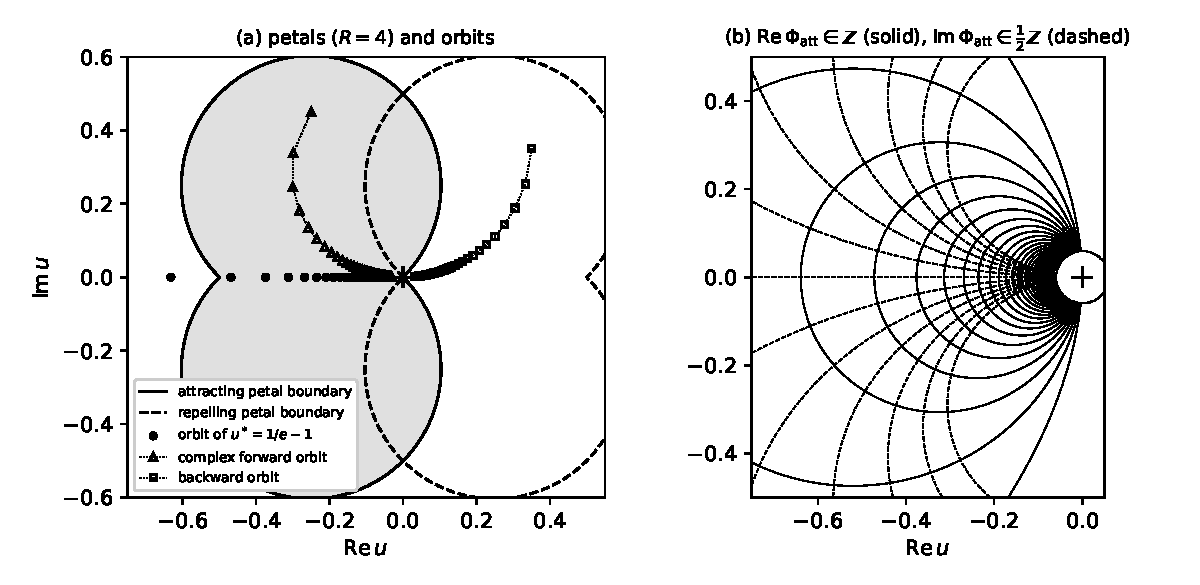
\includegraphics[width=\textwidth]{figures/fig3_petals.pdf}
\caption{$g(u)=\ee^u-1$。(a) 吸引花瓣（灰色，实线边界）与排斥花瓣（虚线边界），取示意值
$R=4$（$\zeta=-2/u$）；实心点是 $\ustar=1/\ee-1$ 的实轨道，三角是一条复轨道，二者沿负实轴切向趋于
$0$；方块是一条后向轨道，沿正实轴趋于 $0$。(b) $\Phiatt$ 的坐标网：实线 $\Rea\Phiatt\in\Z$，
虚线 $\Ima\Phiatt\in\frac12\Z$；相邻两条实线之间是 $g$ 的一个基本域。脚本
\texttt{figures/fig3\_petals.py}。}\label{ch3:fig:petals}
\end{figure}

%======================================================================
\notes

\paragraph{花瓣与 Fatou 坐标。} 花瓣定理属于 Leau（1897）与 Fatou \cite{Fatou1919}。
本章的证明在坐标 $\zeta=-1/(a_2u)$ 中把一切归结为「近似平移」$G(\zeta)=\zeta+1+O(1/\zeta)$，
这是 Milnor \cite[\S10]{Milnor2006} 与 Carleson--Gamelin \cite[第 II 章]{CarlesonGamelin1993}
的做法；我们只处理重数为 $2$ 的情形，此时只有一对花瓣，并且用 $s,t$ 两个线性函数给出了显式的
花瓣与增长率。Fatou 坐标用形式 Abel 函数归一化的写法见 Loray \cite{Loray2006} 与
Buff--Epstein \cite{BuffEpstein2002}；对 $\ee^u-1$ 的极限公式 $\Phiatt=\lim[\alpha(f^nu)-n]$
见 \cite[\S2.1]{KneserPaper}。迭代留数（résidu itératif）的名称来自 Écalle。

\paragraph{horn 映射与分类。} 解析分类定理属于 Écalle \cite{Ecalle1981} 与
Voronin \cite{Voronin1981}；「horn 映射」的名称来自复动力系统中的抛物内爆理论
（Douady、Lavaurs \cite{Lavaurs1989}、Shishikura \cite{Shishikura2000}）。
\Cref{ch3:thm:ecalle-voronin}(2) 的粘合证明是标准的；实现部分 (3) 我们只引用。不同文献对 horn
映射的方向（$\Phirep\circ\Phiatt^{-1}$ 还是其逆）、Fatou 坐标的加性常数、以及下 horn 映射常数项
的符号有不同的约定。本书的约定与论文一致：
$\horn^{-1}=\Phiatt\circ\Phirep^{-1}=z+\sum B_n\ee^{2\pi\ii nz}$，两侧都用 $\alpha$ 归一化。
论文把上 horn 映射的系数记为 $A_n$；本书改记为 $\tilde B_n$，以免与第 4 章的留数 $A_j$ 冲突。
论文 Remark~2.7 中柱面芽的系数与迭代留数也记作 $a_2,a_3,\rho$，本书记为 $\rho_H$。

\paragraph{$B_1\ne0$。} \Cref{prop:B1-nonzero} 的论证来自 \cite[Prop.~2.4、Remark~2.5]{KneserPaper}，
关键输入是 Chéritat 对单奇值类的抛物重整化 \cite{Cheritat2022}，背后的机制是 Epstein 的有限型
理论 \cite{Epstein1993}。近抛物重整化的另一套框架见 Inou--Shishikura \cite{InouShishikura}。

\paragraph{与论文的对应。} \cref{ch3:sec:fatou} 对应 \cite[\S2.1]{KneserPaper} 的前半与
\cite[\S4, Lemma~4.2、4.3]{KneserPaper} 在 $b=\eta$ 处的特例；\cref{ch3:prop:horn-expansion} 对应
\cite[\S4, (d)]{KneserPaper}；\cref{ch3:prop:normalisation}(3) 对应 \cite[Prop.~9.6]{KneserPaper}（基点无关性）在抛物侧的
部分；\cref{ch3:sec:examples} 的数值来自 \cite[\S2.1、Prop.~2.6、附录 A]{KneserPaper} 与
\texttt{docs/generality-check-zh.md} §2.1。论文的节号与定理号按投稿稿 \texttt{main.tex} 编译后的编号引用，对应源文件中的
标签 \texttt{sec:horn}、\texttt{eq:B12}、\texttt{prop:horn-nonzero}、\texttt{prop:horn-intervals}、
\texttt{rem:formal}、\texttt{sec:proofC}、注~9.5（\texttt{rem:gen-B1}） 为准。

%======================================================================
\exercises

\begin{exercise}\label{ch3:exe:mobius}
设 $g(u)=u/(1-u)$。验证 $\rho=0$，$\alpha(u)=-1/u$ 精确成立，$\Phiatt=\Phirep=-1/u$，
并且上、下 horn 映射都是恒等映射。
\end{exercise}

\begin{exercise}\label{ch3:exe:quadG}
对 $g(u)=u+u^2$ 验证 $G(\zeta)=\zeta+1+1/(\zeta-1)$，并据此对 $|\zeta|\ge4$ 给出\cref{ch3:lem:zeta}
中 $C_1$ 的一个显式值。
\end{exercise}

\begin{exercise}\label{ch3:exe:rho-iterate}
(1) 证明 $g^{\circ2}$ 的迭代留数是 $\rho/2$，更一般地 $g^{\circ m}$ 的是 $\rho/m$；并验证 $\alpha/m$
是 $g^{\circ m}$ 的形式 Abel 函数。(2) 证明 $\breve g(v):=-g^{-1}(-v)$ 是二重抛物芽，
$a_2(\breve g)=a_2$，$\rho(\breve g)=-\rho$。
\end{exercise}
\begin{hint}
(2) 用 \eqref{ch3:eq:ginv}。
\end{hint}

\begin{exercise}\label{ch3:exe:d1}
推导 \eqref{ch3:eq:d1}，并验证 $\ee^u-1$ 与 $u+u^2$ 的 $d_1$ 分别为 $-1/36$ 与 $-1/2$。
\end{exercise}

\begin{exercise}\label{ch3:exe:Btilde}
从 $\horn\circ\horn^{-1}=\id$ 推出 $\tilde B_3$ 用 $B_1,B_2,B_3$ 的表达式。
\end{exercise}

\begin{exercise}\label{ch3:exe:nonunique}
令 $\Phi=\Phiatt+\frac{1}{2\pi}\sin(2\pi\Phiatt)$。证明 $\Phi\circ g=\Phi+1$，但 $\Phi$ 不是 Fatou
坐标。\Cref{thm:fatou-coordinates}(4) 的哪个条件不成立？
\end{exercise}
\begin{hint}
由\cref{thm:fatou-coordinates}(3)，$\Ima\Phiatt$ 在 $\Patt(R)$ 上无界。
\end{hint}

\begin{exercise}\label{ch3:exe:real}
设 $g$ 是实芽。由\cref{thm:fatou-coordinates}(7)，$\Phiatt$ 在 $\Patt(R)\cap\R$ 上取实值。证明它在那里
严格递增；从而若 $\ustar<0$ 在直接吸引域的实区间中，则 $a=\Phiatt(\ustar)\in\R$。
\end{exercise}

\begin{exercise}\label{ch3:exe:orbit}
对 $\ee^u-1$ 与 $u_0=-1$，从\cref{ch3:cor:orbit} 推出\cref{ch3:ex:orbit} 中的极限
$2(a-1)-\tfrac23\log2$，并估计 $n=10^5$ 时的误差阶。
\end{exercise}

\begin{exercise}\label{ch3:exe:cylinder}
设 $B_1\ne0$，$H(q)=q\exp(2\pi\ii\sum_{n\ge1}B_nq^n)$。证明 $H$ 的迭代留数 $\rho_H$ 满足
$B_2/B_1^2=2\pi\ii(\tfrac12-\rho_H)$，并用\cref{ch3:tab:horn} 算出 $\ee^u-1$ 与 $u+u^2$ 的 $\rho_H$。
\end{exercise}

\begin{exercise}\label{ch3:exe:normal-form}
令 $X=\frac{a_2u^2}{1+\rho a_2u}\partial_u$，$\phi_X$ 为其时间一映射。
(1) 证明 $T(u)=-1/(a_2u)+\rho\log(-u)$ 满足 $T'=1/X$，从而 $T\circ\phi_X=T+1$，$\phi_X$ 的
迭代留数为 $\rho$。(2) 证明存在形式变换 $h(u)=u+O(u^2)$ 使 $T\circ h=\alpha+\mathrm{const}$，并由此
推出 $h\circ g=\phi_X\circ h$（形式上）。(3) 证明 $\phi_X$ 的上、下逆 horn 映射分别为 $z$ 与
$z+2\pi\ii\rho$。
\end{exercise}
\begin{hint}
(2) 比较 $T(u(1+h_1u+h_2u^2+\cdots))$ 与 $\alpha(u)$ 的 $u^{k-1}$ 项：$h_k$ 以系数 $1/a_2$ 出现，其余
只含 $h_1,\dots,h_{k-1}$。(3) $T$ 在两片花瓣上就是 Fatou 坐标。
\end{hint}

\begin{exercise}\label{ch3:exe:embed}
（较难）证明：若 $B_n=0$ 且 $B_{-n}=0$ 对所有 $n\ge1$ 成立，则 $g$ 解析共轭于习题~\ref{ch3:exe:normal-form}
中的 $\phi_X$，从而 $g$ 可以嵌入一个全纯向量场的流。
\end{exercise}
\begin{hint}
用\cref{ch3:thm:ecalle-voronin}(2)，取 $g_1=\phi_X$，$\kappa=0$。
\end{hint}

\begin{exercise}\label{ch3:exe:residue-analytic}
（较难）不经过形式计算，直接证明 $\rho$ 是解析共轭不变量：对任意使 $\Phirep$ 在 $\Prep(R)$ 上单值的
归一化，上、下逆 horn 映射的常数项之差都等于 $2\pi\ii\rho$。
\end{exercise}
\begin{hint}
常数项之差在 $\Phiatt\mapsto\Phiatt+c_{\mathrm a}$、$\Phirep\mapsto\Phirep+c_{\mathrm r}$ 下不变（\cref{ch3:prop:normalisation}(1)）。
对 $\alpha_0$ 归一化的坐标，用 \eqref{ch3:eq:same-alpha}。
\end{hint}

% 第 4 章 实鞍结开折
% 来源：docs/paper-submission/sec-general.tex（Prop. gen-scale 及改写清单）；
%       docs/paper-submission/main.tex Lemma param、Prop. saddle、Lemma res、Lemma F；
%       docs/general-statements-zh.md §1--§2.1；docs/generality-check-zh.md §1。
% 数值：figures/ch04_scales.py。

\chapter{实鞍结开折}\label{ch:unfolding}

第~\ref{ch:koenigs}、\ref{ch:fatou} 章分别处理了一个双曲不动点和一个抛物不动点。
本章把两者放进同一个单参数族：参数 $s>0$ 时有两个靠得很近的实双曲不动点，
$s=0$ 时它们合并成一个二重抛物不动点。这样的族叫做\textbf{实鞍结开折}
（real saddle-node unfolding）。从第~\ref{ch:transition} 章到第~\ref{ch:variation} 章，
全部结果都在本章的假设 (H1)--(H5) 下陈述和证明。

本章只做准备工作，不涉及分数次迭代本身。我们要回答三个定量问题：
两个乘子离 $1$ 有多远；两个 Koenigs 坐标的虚周期之差趋于什么；
用什么函数作为``两个不动点同时存在时''的近似 Abel 坐标。答案分别是
\cref{prop:scales}、\cref{lem:residues} 和模型时间 $\Psi_s$。
它们都只依赖于芽的两个系数 $a_2$、$\rho$ 和开折的一个系数 $\gamma$。

\begin{goals}
\item 实鞍结开折的定义 (H1)--(H5)，四个例子，以及 Glutsyuk 方向与 Lavaurs 方向的区别。
\item Weierstrass 预备定理把 $f_s(u)-u$ 写成二次多项式乘以无零点的因子；判别式 $D(s)=4\gamma s/a_2+O(s^2)$。
\item 尺度：$|\log\lambda_1|$、$\log\lambda_2\approx2\sqrt{a_2\gamma s}$，强迫尺度
  $\Lam=\exp\bigl(-2\pi^2/\sqrt{a_2\gamma s}\,(1+o(1))\bigr)$，内蕴参数 $p=4a_2\gamma s+O(s^2)$ 关于 $s$ 全纯。
\item 留数 $A_j=1/\log\lambda_j$ 满足 $A_1+A_2=\rho+O(s)$（它是 $s$ 的全纯函数）、$A_1(u_1-u_2)=1/a_2+O(\sqrt s)$；
  模型时间 $A_1\log(u-u_1)+A_2\log(u-u_2)$ 的一步误差是 $O(|u-u_1||u-u_2|)$，且关于 $s$ 一致。
\item tetration 的具体常数：$C_\eta=4\pi^2/\sqrt{2\ee^{1-1/\ee}}=20.3508\ldots$，以及一张数值表。
\end{goals}

% ======================================================================
\section{定义与例子}\label{ch4:sec:def}

\subsection{假设}

设 $f_s(w)$ 是一个依赖于实参数 $s$ 的映射族。我们总在一个点 $(s,w)=(0,w^*)$ 附近工作，
并取以 $w^*$ 为中心的\textbf{仿射坐标} $u$：
\begin{equation}\label{ch4:eq:affine}
 w=w^*+c\,u,\qquad c>0 .
\end{equation}
一般情形取 $c=1$；tetration 取 $c=\ee$（\cref{ch4:exa:tetration}）。在 $u$ 坐标下把 $f_s$ 写成
\[
 f_s(u):=\frac{f_s(w^*+cu)-w^*}{c}
\]
（同一个字母，按自变量的名字区分坐标）。$s=0$ 时的芽记作
\[
 g(u)=f_0(u)=u+a_2u^2+a_3u^3+\cdots .
\]

\begin{definition}[实鞍结开折]\label{def:unfolding}
称 $(f_s)_s$ 连同一个\textbf{基点}（base point）$w_0\in\R$ 为一个\textbf{实鞍结开折}
（real saddle-node unfolding），如果下列条件成立。
\begin{enumerate}[label=\textup{(H\arabic*)},leftmargin=3.2em]
\item \emph{正则性与实性.} 存在 $s_0>0$，使 $f_s(w)$ 在 $\{|s|<s_0\}\times\C$ 上对 $(s,w)$ 联合全纯，
  对每个 $s$ 是 $w$ 的整函数，并且 $s,w$ 都为实数时 $f_s(w)$ 为实数。
\item \emph{鞍结.} $f_0(w^*)=w^*$，$f_0'(w^*)=1$，且 $f_0''(w^*)>0$。在 $u$ 坐标下这就是
  \[
   a_2:=\tfrac12g''(0)=\tfrac c2f_0''(w^*)>0 .
  \]
\item \emph{横截性.} 在 $u$ 坐标下
  \begin{equation}\label{ch4:eq:direction}
   f_s=g-sX+O(s^2),\qquad X:=-\partial_sf_s\big|_{s=0},
  \end{equation}
  其中 $O(s^2)$ 在 $u$ 的一个固定圆盘上一致。函数 $X$ 叫做开折的\textbf{方向}（direction），
  数
  \[
   \gamma:=X(0)>0
  \]
  叫做\textbf{横截性常数}。
\item \emph{基点.} $w_0<w^*$，并且 $f_0$ 在 $[w_0,w^*]$ 上递增，在 $[w_0,w^*)$ 上满足 $f_0(w)>w$。
  记 $\ustar:=(w_0-w^*)/c<0$ 为基点的 $u$ 坐标。
\item \emph{非退化的 horn 映射.} $B_1\ne0$，其中 $B_n$ 是芽 $g$ 的逆上 horn 映射的 Fourier 系数
  （\cref{def:horn}）。涉及第 $n$ 个系数的对数陈述还要求 $B_n\ne0$。
\end{enumerate}
芽的\textbf{迭代留数}（iterative residue）记作
\[
 \rho:=1-\frac{a_3}{a_2^2}.
\]
$a_2,a_3,X,\gamma$，以及第~\ref{ch:fatou} 章的 Fatou 坐标、$B_n$ 与基点的 Fatou 值 $a:=\Phiatt(\ustar)$，都在 $u$ 坐标中计算。
\end{definition}

\begin{remark}[仿射坐标的选择]\label{ch4:rem:affine}
把 $c$ 换成 $c'=\mu c$（$\mu>0$），即 $u=\mu u'$，芽变成 $\mu^{-1}g(\mu u')$：$a_2\mapsto\mu a_2$，$a_3\mapsto\mu^2a_3$，$X\mapsto X(\mu\,\cdot)/\mu$，
$\gamma\mapsto\gamma/\mu$。所以 $\rho$、$a_2\gamma$ 以及乘子都与 $c$ 无关。$a$ 与 $B_n$ 的辐角依赖于 $c$，
但乘积 $B_n\ee^{2\pi\ii na}$ 与 $c$ 无关；$a$ 是实数，所以 $|B_n|$ 也与 $c$ 无关（第~\ref{ch:fatou} 章关于缩放的注）。
第~\ref{ch:transition} 章以后出现的不变量 $\tau_n$、$|B_n|$、$\Rea\kappa^{(n)}_j$ 都与 $c$ 的选取无关。
\end{remark}

\begin{remark}[符号约定]\label{ch4:rem:signs}
(H2) 中的 $a_2>0$ 与 (H3) 中的 $\gamma>0$ 都只是约定。若 $a_2<0$，用 $w\mapsto 2w^*-w$ 共轭；
若 $\gamma<0$，把 $s$ 换成 $-s$。两者都不改变问题。约定 $a_2>0$ 使吸引花瓣在 $u<0$ 一侧
（第~\ref{ch:fatou} 章），约定 $\gamma>0$ 使 $s>0$ 一侧有两个实不动点（\cref{ch4:lem:real-dynamics}）。
\end{remark}

\begin{remark}[各条假设的作用]\label{ch4:rem:roles}
\begin{enumerate}
\item (H1) 中的``整函数''只用来保证排斥不动点处的正则解 $S$ 是整函数（第~\ref{ch:transition} 章）。
  其余论证都发生在 $w^*$ 的一个固定小圆盘里，联合全纯性只在这个圆盘上用到。
  特别地，本书的局部理论\emph{不需要任何全局假设}。
\item (H3) 中的符号条件是：在 $u$ 坐标下 $\partial_sf_s(0)|_{s=0}=-\gamma<0$（在 $w$ 坐标下是 $-c\gamma$）。参数增大时，鞍结点处的值往下移。
  方向 $X$ 的其余部分 $X-X(0)$ 在第~\ref{ch:variation} 章才起作用。
\item (H4) 保证基点落在吸引不动点的直接吸引域中、并且在吸引不动点的``远侧''（\cref{ch4:lem:real-dynamics}(4)）。
  第~\ref{ch:transition} 章将看到，这正是``缝口在实轴下方半个周期''的来源。
\item (H5) 只用于比值 $t_n/t_1^n$、$c_n/c_1^n$ 和对数形式的展开。汇流定理、缝合解和不变性命题都不需要它。
\end{enumerate}
\end{remark}

\subsection{例子}

\begin{example}[tetration]\label{ch4:exa:tetration}
设 $1<b<\eta:=\ee^{1/\ee}$，$E(w)=b^w$。令
\[
 s:=1-\ee\log b .
\]
$s=0$ 时 $E(w)=\eta^w$，不动点 $w^*=\ee$，$E'(\ee)=1$。为了使芽取最简单的形式，取仿射坐标 $w=\ee(1+u)$，即 $c=\ee$。则
\[
 f_s(u)=\frac{E(\ee+\ee u)-\ee}{\ee}=\ee^{-s+(1-s)u}-1,\qquad g(u)=\ee^u-1=u+\tfrac12u^2+\tfrac16u^3+\cdots .
\]
所以 $a_2=\tfrac12$，$a_3=\tfrac16$，$\rho=1-\tfrac{1/6}{1/4}=\tfrac13$。方向是
$X(u)=-\partial_sf_s|_{s=0}=(1+u)\ee^u$，$\gamma=1$。tetration 的归一化 $F(0)=1$ 对应基点
$w_0=1$，即 $\ustar=1/\ee-1$，$a=\Phiatt(1/\ee-1)=3.0292972144180\ldots$（\cite{KneserPaper}，有区间证书）。
(H4) 成立，因为 $\eta^w$ 递增且 $w<\ee$ 时 $\eta^w>w$。
(H5) 是 \cref{prop:B1-nonzero}。$s>0$ 对应 $b<\eta$，$s<0$ 对应 $b>\eta$。
\end{example}

以后说 tetration 时，总是指 \cref{ch4:exa:tetration} 的 $u$ 坐标 $w=\ee(1+u)$。
若改用 $c=1$（$u=w-\ee$），则 $a_2=\frac1{2\ee}$、$\gamma=\ee$，$a$ 与 $B_n$ 都变，但 $B_n\ee^{2\pi\ii na}$ 不变（\cref{ch4:rem:affine}）。

\begin{example}[另外三个族]\label{ch4:exa:families}
下列三个族取自 \cite{KneserPaper} 的一般化检验（\texttt{docs/generality-check-zh.md} §1）。
\begin{enumerate}
\item \emph{二次族} $w^2+c$，$c\uparrow\frac14$。$w^*=\frac12$，$s=\frac14-c$，
  $f_s(u)=u+u^2-s$，所以 $g(u)=u+u^2$，$a_2=1$，$a_3=0$，$\rho=1$，$X\equiv1$，$\gamma=1$。
  不动点 $u_{1,2}=\mp\sqrt s$，乘子 $1\mp2\sqrt s$。基点可取 $w_0=0.2$；
  $w_0=0$（临界点）也满足 (H4)：$f_0'(w)=2w$ 只在端点 $w=0$ 处为零，$f_0$ 在 $[0,\frac12]$ 上仍严格递增。
\item \emph{正弦族} $v-\sin v+c$，$c\uparrow1$。$v^*=\pi/2$，$s=1-c$，
  $f_s(u)=u+1-\cos u-s$，$g(u)=u+\frac{u^2}2-\frac{u^4}{24}+\cdots$，所以 $a_2=\frac12$，$a_3=0$，$\rho=1$，
  $X\equiv1$，$\gamma=1$。不动点 $\arcsin c$ 与 $\pi-\arcsin c$，乘子 $1\mp\sqrt{1-c^2}$。基点取 $v_0=0.8$。
\item \emph{退化留数族} $w+(w^2-c)\ee^w$，$c\downarrow0$。$w^*=0$，$s=c$，
  $f_s(u)=u+(u^2-s)\ee^u$，$g(u)=u+u^2\ee^u$，所以 $a_2=a_3=1$，$\rho=0$，$X=\ee^u$，$\gamma=1$。
  不动点 $\mp\sqrt s$，乘子 $1-2\sqrt s\,\ee^{-\sqrt s}$ 与 $1+2\sqrt s\,\ee^{\sqrt s}$。基点取 $w_0=-0.8$。
\end{enumerate}
前两族的乘子满足 $\lambda_1+\lambda_2=2$；第三族没有这个对称性。$\rho=0$ 的芽的形式 Abel 函数没有对数项。
\end{example}

\Cref{ch4:tab:families} 汇总这些数据。最后一列是逆 horn 映射的第一个系数的模，来自
\cite[注~9.14]{KneserPaper}（数值，60 位运算）；第一行另有区间证书（\cref{ch:numerics}）。

\begin{table}[htbp]
\centering
\caption{四个实鞍结开折。$|B_1|$ 一列为数值（\texttt{generality\_check.py}）。}
\label{ch4:tab:families}
\small
\begin{tabular}{lllllll}
\toprule
族 & $s$ & $g(u)$ & $a_2$ & $\rho$ & $X$ & $|B_1|$\\
\midrule
$b^w$（$w=\ee(1+u)$） & $1-\ee\log b$ & $\ee^u-1$ & $1/2$ & $1/3$ & $(1+u)\ee^u$ & $0.0890584364122$\\
$w^2+c$ & $\tfrac14-c$ & $u+u^2$ & $1$ & $1$ & $1$ & $0.0597942361690$\\
$v-\sin v+c$ & $1-c$ & $u+1-\cos u$ & $1/2$ & $1$ & $1$ & $0.0723786416245$\\
$w+(w^2-c)\ee^w$ & $c$ & $u+u^2\ee^u$ & $1$ & $0$ & $\ee^u$ & $2744.09379131$\\
\bottomrule
\end{tabular}
\end{table}

\begin{remark}[(H5) 在各例中的状态]\label{ch4:rem:H5}
对 tetration，(H5) 是 \cref{prop:B1-nonzero}。那里的证明只用到：$g$ 限制在直接抛物吸引域上恰有一个奇异值。
二次族的直接吸引域里只有一个临界点，同一论证适用（\cite[注~9.5]{KneserPaper}）。
正弦族的临界值 $2\pi k+1$ 都是实数，只有 $k=0$ 那一个落在直接吸引域内，但 $g$ 不是有限型的，
论证能否照搬需要另外检查。对第三族，目前只有数值事实 $|B_1|\approx2744\ne0$。
所以在一般理论中，(H5) 保留为假设。
\end{remark}

\subsection{两个方向：Glutsyuk 与 Lavaurs}

一个鞍结开折在 $s=0$ 两侧的行为完全不同（\cref{ch4:lem:prep} 之后可以精确叙述）。
\begin{itemize}
\item $s>0$：两个实不动点 $u_1<u_2$，一个吸引一个排斥，乘子是 $1$ 附近的正实数。
  这是本书研究的一侧。在开折理论的文献中，沿这一侧趋于 $s=0$ 的极限称为 \textbf{Glutsyuk 方向}
  （Glutsyuk direction）：两个双曲不动点各自的线性化坐标收敛到抛物芽的两个扇形 Fatou 坐标
  \cite{Glutsyuk2001}。第~\ref{ch:confluence} 章证明的汇流定理就是这一类命题。
\item $s<0$：两个不动点是一对共轭复数，乘子 $1\pm\ii a_2\sqrt{|D(s)|}+O(s)$ 位于 $1$ 附近、
  几乎在单位圆上。实轴上的轨道从两个不动点之间的``门''穿过去。沿这一侧趋于 $s=0$ 的极限称为
  \textbf{Lavaurs 方向}，对应经典的抛物内爆（parabolic implosion）\cite{Lavaurs1989,Shishikura2000,Oudkerk1999}。
\end{itemize}
\Cref{ch4:fig:unfolding} 画出了 tetration 的 $f_s(u)-u$ 在三种 $s$ 下的图像。
对 tetration，$s<0$ 就是 $b>\eta$：Kneser 的经典构造正是在这一侧进行的。

\begin{figure}[htbp]
\centering
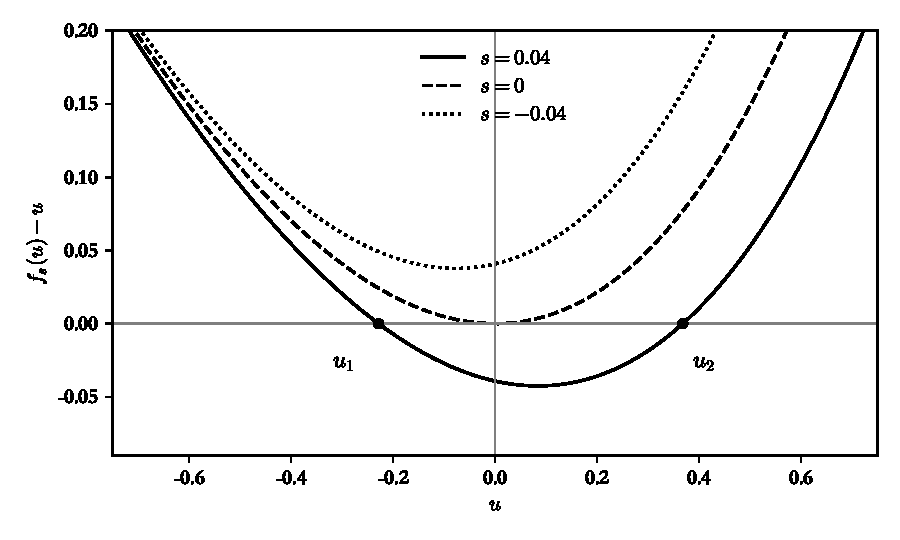
\includegraphics[width=0.7\textwidth]{figures/fig4_unfolding.pdf}
\caption{tetration 开折的 $f_s(u)-u$，$f_s(u)=\ee^{-s+(1-s)u}-1$（\texttt{figures/fig4\_unfolding.py}）。
$s=0.04$：两个实零点 $u_1=-0.2283$、$u_2=0.3683$（Glutsyuk 一侧）；$s=0$：二重零点；$s=-0.04$：没有实零点（Lavaurs 一侧）。}
\label{ch4:fig:unfolding}
\end{figure}
开折的完整解析分类（在 $0$ 的整个复邻域上）见 \cite{MRR2004,ChristopherRousseau}。
本书只在 $s>0$ 一侧工作，复参数只在第~\ref{ch:examples} 章出现。

% ======================================================================
\section{Weierstrass 预备与实动力学}\label{ch4:sec:prep}

\subsection{预备式与判别式}

记 $D_r=\{|u|<r\}$。

\begin{lemma}[预备式]\label{ch4:lem:prep}
设 (H1)--(H3) 成立。存在 $r>0$ 和 $s_1\in(0,s_0)$，使得对 $|s|<s_1$、$|u|<r$，
\begin{equation}\label{ch4:eq:prep}
 f_s(u)-u=q_s(u)\,k_s(u),\qquad q_s(u)=u^2-\beta_1(s)u+\beta_2(s),
\end{equation}
其中
\begin{enumerate}
\item $\beta_1,\beta_2$ 在 $|s|<s_1$ 上全纯，$s$ 为实数时取实值，$\beta_1(0)=\beta_2(0)=0$；
\item $k$ 在 $\{|s|<s_1\}\times\overline{D_r}$ 上联合全纯、无零点，$s,u$ 为实数时取实值，并且
  \[
   k_0(u)=a_2+a_3u+O(u^2),\qquad k_0(0)=a_2,\quad k_0'(0)=a_3 ;
  \]
\item 判别式 $D(s):=\beta_1(s)^2-4\beta_2(s)$ 满足
  \begin{equation}\label{ch4:eq:disc}
   D(s)=\frac{4\gamma}{a_2}\,s+O(s^2),\qquad \beta_2(s)=-\frac{\gamma}{a_2}s+O(s^2),\qquad \beta_1(s)=O(s).
  \end{equation}
\end{enumerate}
特别地，$f_s$ 在 $D_r$ 中恰有两个不动点（计重数），即 $q_s$ 的两个根
$u_{1,2}=\tfrac12\bigl(\beta_1\mp\sqrt{D(s)}\bigr)$，并且 $|u_j|\le C\sqrt{|s|}$。
\end{lemma}

\begin{proof}
函数 $F(s,u)=f_s(u)-u$ 在 $(0,0)$ 附近联合全纯，且 $F(0,u)=g(u)-u=u^2(a_2+a_3u+\cdots)$
在 $u=0$ 处有二阶零点。由 Weierstrass 预备定理（\cref{thm:weierstrass-prep}），
存在 $r,s_1$ 和唯一的分解 $F=q\cdot k$，其中 $q$ 是首一二次 Weierstrass 多项式，
系数在 $s=0$ 处为零，$k$ 在闭双圆盘上无零点。由唯一性，$\overline{F(\bar s,\bar u)}=F(s,u)$
推出 $q$、$k$ 都有同样的实对称性，即 (1)、(2) 中的实性。$s=0$ 时 $q_0(u)=u^2$，
所以 $k_0(u)=(g(u)-u)/u^2=a_2+a_3u+\cdots$。

在 $u=0$ 处取值：$f_s(0)=\beta_2(s)k_s(0)$。由 (H3)，$f_s(0)=g(0)-sX(0)+O(s^2)=-\gamma s+O(s^2)$；
而 $k_s(0)=a_2+O(s)$。所以 $\beta_2=-\gamma s/a_2+O(s^2)$。$\beta_1$ 全纯且 $\beta_1(0)=0$，故
$\beta_1=O(s)$，$\beta_1^2=O(s^2)$。这给出 \eqref{ch4:eq:disc}。

$k$ 无零点，所以 $D_r$ 中的不动点恰为 $q_s$ 的根。最后，$|\beta_1|\le C|s|$ 且
$|D(s)|\le C|s|$，故 $|u_j|\le C\sqrt{|s|}$（缩小 $s_1$ 使根落在 $D_{r/2}$ 内）。
\end{proof}

以后固定 \cref{ch4:lem:prep} 中的 $r$、$s_1$。由 $k$ 的连续性，可以再缩小 $r$、$s_1$，使得
\begin{equation}\label{ch4:eq:k-bounds}
 \tfrac12a_2\le|k_s(u)|\le2a_2,\qquad |k_s(u)-a_2|\le C(|s|+|u|),\qquad
 |f_s'(u)-1|\le\tfrac14
 \qquad(|s|<s_1,\ |u|<r).
\end{equation}

\subsection{$s>0$ 时的实动力学}

把 $u$ 坐标下的两个不动点换回 $w$ 坐标，记 $L=w^*+cu_1$、$L_2=w^*+cu_2$。为了记号简单，
本节的证明中取 $c=1$；一般情形只差一个正的伸缩，所有单调性与符号都不变。

\begin{lemma}[实动力学]\label{ch4:lem:real-dynamics}
设 (H1)--(H4) 成立。存在 $s_2\in(0,s_1)$，使得对每个 $s\in(0,s_2]$：
\begin{enumerate}
\item $D(s)>0$，两个不动点 $u_1<u_2$ 都是实数，$u_2-u_1=\sqrt{D(s)}$；
\item 它们的乘子
  \begin{equation}\label{ch4:eq:multipliers}
   \lambda_1=f_s'(u_1)=1-\sqrt{D}\,k_s(u_1),\qquad \lambda_2=f_s'(u_2)=1+\sqrt{D}\,k_s(u_2)
  \end{equation}
  满足 $0<\lambda_1<1<\lambda_2$；
\item $f_s$ 在实区间 $[L,L_2]$ 上严格递增，在 $(L,L_2)$ 上 $f_s(w)<w$。于是 $(L,L_2)$ 中每个点的轨道
  递减地趋于 $L$，区间 $(L,L_2)$ 落在 $L$ 的直接吸引域中；
\item $w_0<L$，$f_s$ 把 $[w_0,L)$ 映入自身，并且 $[w_0,L)$ 中每个点的轨道递增地趋于 $L$。
  特别地 $w_0$ 落在 $L$ 的直接吸引域中；
\item 设 $\sigma$ 是 $L$ 处的 Koenigs 坐标，$\sigma\circ f_s=\lambda_1\sigma$，$\sigma'(L)=1$
  （\cref{thm:koenigs}），延拓到整个吸引域上。则 $\sigma$ 在 $[w_0,L)$ 上为负，在 $(L,L_2)$ 上为正。
\end{enumerate}
\end{lemma}

\begin{proof}
(1) 由 \eqref{ch4:eq:disc}，$D(s)=\frac{4\gamma}{a_2}s(1+O(s))>0$。$\beta_j$ 实，所以两根实且相差 $\sqrt D$。

(2) 对 \eqref{ch4:eq:prep} 求导并在 $u_1$ 处取值：$f_s'(u_1)-1=q_s'(u_1)k_s(u_1)=(u_1-u_2)k_s(u_1)$；
$u_2$ 同理。由 \eqref{ch4:eq:k-bounds}，$k_s(u_j)$ 是接近 $a_2>0$ 的正实数，$\sqrt D$ 很小，
所以 $0<\lambda_1<1<\lambda_2$。

(3) 由 \eqref{ch4:eq:k-bounds}，$f_s'\ge\frac34$ 在 $D_r\cap\R$ 上成立，而 $[u_1,u_2]\subset D_r$。
在 $(u_1,u_2)$ 上 $q_s<0$、$k_s>0$，故 $f_s(u)<u$；又 $f_s(u)>f_s(u_1)=u_1$。所以
$f_s\bigl((u_1,u_2)\bigr)\subset(u_1,u_2)$，轨道单调递减、有下界 $u_1$，极限是 $[u_1,u_2)$ 中的不动点，只能是 $u_1$。
连通集 $[L,L_2)$ 落在吸引域中并含 $L$，所以落在直接吸引域中。

(4) 取 $\delta\in(0,r)$ 很小，使 $f_0(w^*-\delta)<w^*-\delta/2$（这由 $g(-\delta)=-\delta+a_2\delta^2+\cdots$ 推出）。
由 (H4)，$f_0(w)-w$ 在紧区间 $[w_0,w^*-\delta]$ 上有正的下界，$f_0$ 在其上递增，因而
$f_0([w_0,w^*-\delta])\subset(w_0,w^*-\delta/2]$。由连续性，$s$ 充分小时
$f_s(w)>w$ 在 $[w_0,w^*-\delta]$ 上成立，并且 $f_s([w_0,w^*-\delta])\subset(w_0,w^*-\delta/4)$。
再由 $|u_1|\le C\sqrt s$，$s$ 充分小时 $w^*-\delta/4<L$。另一方面，在 $[w^*-\delta,L)$ 上，
$q_s(u)>0$（$u<u_1<u_2$）、$k_s>0$，故 $f_s(w)>w$；$f_s$ 在这一段上递增，故 $f_s(w)<f_s(L)=L$。
合起来，$f_s$ 把 $[w_0,L)$ 映入 $[w_0,L)$，并且其上 $f_s(w)>w$。轨道递增有上界 $L$，极限是
$[w_0,L]$ 中的不动点；而 $[w_0,L)$ 中没有不动点，所以极限为 $L$。直接吸引域的论证同 (3)。

(5) 设 $w\in[w_0,L)$。对 $n$ 充分大，$f_s^n(w)$ 落在 $L$ 的一个小邻域里，并且 $f_s^n(w)<L$。
在这个邻域里 $\sigma$ 是实的、递增的（$\sigma'(L)=1$），$\sigma(L)=0$，所以 $\sigma(f_s^nw)<0$，
从而 $\sigma(w)=\lambda_1^{-n}\sigma(f_s^nw)<0$。对 $w\in(L,L_2)$，同样的论证给出 $\sigma(w)>0$。
\end{proof}

\begin{remark}\label{ch4:rem:far-side}
(4)、(5) 是 (H4) 的全部用处：基点在吸引不动点 $L$ 的``远离 $L_2$ 的一侧''，而线段 $(L,L_2)$
在另一侧。$\sigma$ 在两侧的符号相反，这就是第~\ref{ch:transition} 章 \cref{lem:realT} 中
$\Ima T\equiv h/2\pmod h$ 的来源。基点落在 $(L,L_2)$ 中会是什么情形，没有研究过。
\end{remark}

\subsection{反射逆}

第~\ref{ch:confluence} 章处理排斥不动点时，要把 $f_s$ 的局部逆``翻转''成一个吸引的映射。

\begin{lemma}[反射逆]\label{ch4:lem:reflected}
缩小 $r,s_1$ 后，$f_s$ 在 $D_r$ 上单叶。令
\[
 \check f_s(v):=-f_s^{-1}(-v)
\]
（$f_s^{-1}$ 取 $D_r$ 上的局部逆）。则 $\check f_s$ 对 $(s,v)$ 联合全纯，$s$、$v$ 实时取实值；
$\check f_s$ 的不动点是 $-u_2<-u_1$，前者吸引、乘子 $1/\lambda_2$，后者排斥、乘子 $1/\lambda_1$；
$s=0$ 时它的芽是
\[
 \check g(v)=v+a_2v^2+(2a_2^2-a_3)v^3+O(v^4),
\]
迭代留数为 $-\rho$。$\check f_s$ 满足 \eqref{ch4:eq:prep} 型的预备式，横截性常数仍为 $\gamma$。
\end{lemma}

\begin{proof}
由 \eqref{ch4:eq:k-bounds}，$\Rea f_s'\ge\frac34$ 在凸集 $D_r$ 上成立，故 $f_s$ 在 $D_r$ 上单叶
（Noshiro--Warschawski）；局部逆由隐函数定理对 $(s,v)$ 联合全纯。不动点和乘子直接验证。
$g^{-1}(u)=u-a_2u^2+(2a_2^2-a_3)u^3+O(u^4)$（逐阶代入 $g(g^{-1}(u))=u$），
所以 $\check g(v)=-g^{-1}(-v)=v+a_2v^2+(2a_2^2-a_3)v^3+\cdots$，迭代留数
$1-(2a_2^2-a_3)/a_2^2=-1+a_3/a_2^2=-\rho$。最后，$\check f_s(0)=-f_s^{-1}(0)$，
而 $f_s^{-1}(0)=\gamma s+O(s^2)$（由 $f_s(0)=-\gamma s+O(s^2)$ 与 $f_s'(0)=1+O(s)$），
所以 $\check f_s(0)=-\gamma s+O(s^2)$，横截性常数仍为 $\gamma$。
\end{proof}

% ======================================================================
\section{乘子与尺度}\label{ch4:sec:scales}

以下总设 $s\in(0,s_2]$，并沿用 \cref{ch4:lem:real-dynamics} 的记号。
回忆第~\ref{ch:koenigs} 章：吸引正则解 $R$ 的虚周期是 $h=2\pi/|\log\lambda_1|$，
排斥正则解 $S$ 的虚周期是 $h_2=2\pi/\log\lambda_2$。定义
\begin{equation}\label{ch4:eq:Lam-p}
 \Lam:=\exp\Bigl(\frac{4\pi^2}{\log\lambda_1}\Bigr)=\ee^{-2\pi h},\qquad
 p:=-\log\lambda_1\cdot\log\lambda_2 .
\end{equation}
$\Lam$ 叫做\textbf{强迫尺度}（forcing scale），$p$ 叫做\textbf{内蕴参数}（intrinsic parameter）。
$p$ 只依赖于两个乘子，因而在共轭和重新参数化下不变；这是用 $p$ 而不用 $s$ 作展开变量的原因
（第~\ref{ch:first-order} 章）。

为了证明 $p$ 关于 $s$ 全纯，需要一个关于对称函数的简单引理。

\begin{lemma}[根的幂和]\label{ch4:lem:power-sums}
设 $\phi(s,u)$ 在 $\{|s|<s_1\}\times\overline{D_r}$ 上联合全纯。则
\[
 \Sigma_\phi(s):=\phi(s,u_1(s))+\phi(s,u_2(s))
\]
在 $|s|<s_1$ 上全纯（$u_{1,2}(s)$ 是 $q_s$ 的两根，$s$ 为复数时也如此定义，重根计两次）。
\end{lemma}

\begin{proof}
两根都在 $D_{r/2}$ 内。由辐角原理，
\[
 \Sigma_\phi(s)=\frac1{2\pi\ii}\oint_{|u|=r}\phi(s,u)\,\frac{q_s'(u)}{q_s(u)}\,\dd u ,
\]
被积函数对 $s$ 全纯、对 $(s,u)$ 连续，且 $|u|=r$ 上 $q_s$ 无零点，所以积分对 $s$ 全纯。
\end{proof}

\begin{proposition}[尺度]\label{prop:scales}
设 (H1)--(H4) 成立。当 $s\to0^+$ 时：
\begin{enumerate}
\item 乘子满足 $\lambda_{1,2}=1\mp a_2\sqrt{D(s)}+O(s)$，并且
  \[
   |\log\lambda_1|,\ \log\lambda_2\;=\;2\sqrt{a_2\gamma s}\,\bigl(1+O(\sqrt s)\bigr);
  \]
\item 强迫尺度满足
  \[
   \Lam=\exp\Bigl(-\frac{2\pi^2}{\sqrt{a_2\gamma s}}\bigl(1+o(1)\bigr)\Bigr),
  \]
  其中 $o(1)$ 实际上是 $O(\sqrt s)$；
\item $p$ 延拓为 $|s|<s_1$ 上的全纯函数，$s$ 实时取实值，并且
  \[
   p=4a_2\gamma\,s+O(s^2);
  \]
  由于 $p'(0)=4a_2\gamma\ne0$，在 $0$ 附近 $s$ 也是 $p$ 的全纯函数，$s=p/(4a_2\gamma)+O(p^2)$；
\item $h_2-h\to2\pi\rho$。更精确地，$h_2-h=2\pi(A_1+A_2)=2\pi\rho+O(s)$，其中 $A_j=1/\log\lambda_j$。
\end{enumerate}
\end{proposition}

\begin{proof}
(1) 由 \eqref{ch4:eq:multipliers} 与 \eqref{ch4:eq:k-bounds}，$k_s(u_j)=a_2+O(|s|+|u_j|)=a_2+O(\sqrt s)$，
故 $\lambda_{1,2}=1\mp\sqrt D\,(a_2+O(\sqrt s))=1\mp a_2\sqrt D+O(s)$（$\sqrt D=O(\sqrt s)$）。
由 \eqref{ch4:eq:disc}，$\sqrt{D}=2\sqrt{\gamma s/a_2}\,(1+O(s))$，于是
$a_2\sqrt D=2\sqrt{a_2\gamma s}\,(1+O(s))$。最后 $\log(1+x)=x(1+O(x))$ 给出
$|\log\lambda_1|=a_2\sqrt D\,(1+O(\sqrt s))=2\sqrt{a_2\gamma s}\,(1+O(\sqrt s))$；$\log\lambda_2$ 同理。

(2) 由 (1)，$\log\lambda_1=-2\sqrt{a_2\gamma s}\,(1+O(\sqrt s))$，所以
\[
 \frac{4\pi^2}{\log\lambda_1}=-\frac{4\pi^2}{2\sqrt{a_2\gamma s}}\bigl(1+O(\sqrt s)\bigr)
 =-\frac{2\pi^2}{\sqrt{a_2\gamma s}}\bigl(1+O(\sqrt s)\bigr).
\]

(3) 由 \eqref{ch4:eq:k-bounds}，$|f_s'(u)-1|\le\frac14$，所以 $\ell_s(u):=\Log f_s'(u)$
（主值对数）在 $\{|s|<s_1\}\times\overline{D_r}$ 上联合全纯。对 $s\in(0,s_2]$，$\lambda_j>0$ 接近 $1$，
所以 $\log\lambda_j=\ell_s(u_j)$。于是
\[
 p=-\ell_s(u_1)\ell_s(u_2)=\tfrac12\Bigl(\Sigma_{\ell^2}(s)-\Sigma_\ell(s)^2\Bigr),
\]
其中 $\Sigma_\ell=\ell_s(u_1)+\ell_s(u_2)$，$\Sigma_{\ell^2}=\ell_s(u_1)^2+\ell_s(u_2)^2$。
由 \cref{ch4:lem:power-sums}，右边在 $|s|<s_1$ 上全纯；我们用它定义 $p$ 在整个圆盘上的延拓。
$\ell$ 的实性给出 $p$ 的实性。$s=0$ 时 $u_1=u_2=0$，$\ell_0(0)=\Log1=0$，所以 $p(0)=0$。
由 (1)，$s\to0^+$ 时 $p(s)/s=4a_2\gamma\,(1+O(\sqrt s))\to4a_2\gamma$，所以 $p'(0)=4a_2\gamma$，
而全纯性给出 $p=p'(0)s+O(s^2)$。$s$ 关于 $p$ 的全纯性是反函数定理。

(4) $h_2-h=2\pi/\log\lambda_2-2\pi/|\log\lambda_1|=2\pi(A_2+A_1)$，因为 $A_1=1/\log\lambda_1=-1/|\log\lambda_1|$。
极限 $A_1+A_2\to\rho$ 及其速率是下一节的 \cref{lem:residues}，它的证明不用 (4)。
\end{proof}

\begin{remark}\label{ch4:rem:scales}
\begin{enumerate}
\item (1) 说明两个乘子以 $\sqrt s$ 的速率离开 $1$，而且一阶上对称：$|\log\lambda_1|$ 与 $\log\lambda_2$
  只在 $O(s)$ 处不同。这一不对称性的主项由 \cref{lem:residues} 精确给出：
  $\frac1{\log\lambda_2}-\frac1{|\log\lambda_1|}=A_1+A_2\to\rho$。
\item (2) 中的 $\Lam$ 比 $s$ 的任何幂都小得多。第~\ref{ch:transition} 章将看到，
  转移映射的第 $n$ 个系数是 $\Lam^{n/2}$ 量级，分离系数 $c_n$ 是 $\Lam^n$ 量级。
\item 由 (3)，$s<0$ 时 $p$ 也有定义。那时两个乘子共轭，$\ell_s(u_2)=\overline{\ell_s(u_1)}$，
  $p=-|\ell_s(u_1)|^2<0$，与 $p\approx4a_2\gamma s$ 一致。
\end{enumerate}
\end{remark}

% ======================================================================
\section{留数与模型时间}\label{ch4:sec:residues}

\subsection{留数}

\begin{lemma}[留数]\label{lem:residues}
设 (H1)--(H4) 成立，$A_j:=1/\log\lambda_j$（于是 $A_1<0<A_2$）。当 $s\to0^+$ 时
\[
 A_1+A_2=\rho+O(s),\qquad A_1(u_1-u_2)=\frac1{a_2}+O(\sqrt s).
\]
更强地，$A_1+A_2$ 延拓为 $|s|<s_1$ 上的全纯函数 $\nu(s)$，$\nu(0)=\rho$。
因此 $A_1u_1+A_2u_2\to1/a_2$，$A_ju_j^2\to0$（$j=1,2$）。
\end{lemma}

\begin{proof}
记 $d=u_1-u_2=-\sqrt{D}$，$k_j=k_s(u_j)$。由 \eqref{ch4:eq:multipliers}，
$\lambda_1=1+dk_1$，$\lambda_2=1-dk_2$。对小的 $x$ 有
\[
 \frac1{\log(1+x)}=\frac1x+\frac12+O(x).
\]
所以
\[
 A_1=\frac1{dk_1}+\frac12+O(d),\qquad A_2=-\frac1{dk_2}+\frac12+O(d),
\]
\[
 A_1+A_2=\frac{k_2-k_1}{d\,k_1k_2}+1+O(d).
\]
由于 $k$ 关于 $(s,u)$ 联合全纯，
\[
 k_2-k_1=k_s(u_2)-k_s(u_1)=(u_2-u_1)\int_0^1\partial_uk_s\bigl(u_1+t(u_2-u_1)\bigr)\dd t
 =-d\,\bigl(a_3+O(\sqrt s)\bigr),
\]
这里用了 $\partial_uk_s(u)=k_0'(0)+O(|s|+|u|)=a_3+O(\sqrt s)$（$|u|\le C\sqrt s$）。又 $k_1k_2=a_2^2+O(\sqrt s)$。故
\[
 A_1+A_2=1-\frac{a_3}{a_2^2}+O(\sqrt s)=\rho+O(\sqrt s).
\]
其次 $A_1d=1/k_1+d/2+O(d^2)=1/a_2+O(\sqrt s)$。最后
$A_1u_1+A_2u_2=A_1(u_1-u_2)+(A_1+A_2)u_2\to1/a_2$，而 $|A_j|\le C/\sqrt s$、$u_j^2=O(s)$ 给出 $A_ju_j^2=O(\sqrt s)$。

\emph{全纯性与速率 $O(s)$.} 沿用 \cref{prop:scales}(3) 的证明中的记号 $\ell_s=\Log f_s'$、$\Sigma_\ell$。
对 $s\in(0,s_2]$，$\log\lambda_j=\ell_s(u_j)$，所以
\[
 A_1+A_2=\frac{\ell_s(u_1)+\ell_s(u_2)}{\ell_s(u_1)\ell_s(u_2)}=-\frac{\Sigma_\ell(s)}{p(s)} .
\]
$\Sigma_\ell$ 在 $|s|<s_1$ 上全纯（\cref{ch4:lem:power-sums}）且 $\Sigma_\ell(0)=2\ell_0(0)=0$；$p$ 全纯，$p(0)=0$，$p'(0)=4a_2\gamma\ne0$。
所以商在 $s=0$ 处的奇点可去（必要时缩小 $s_1$，使 $p$ 在 $0<|s|<s_1$ 上无零点），给出全纯函数 $\nu(s)$。
由上面的极限，$\nu(0)=\rho$，于是 $A_1+A_2=\rho+O(s)$。
\end{proof}

\begin{remark}\label{ch4:rem:residue-rates}
两个速率确实不同。$A_1+A_2$ 在交换两个不动点下对称，因而是 $s$ 的全纯函数，没有 $\sqrt s$ 项；
$A_1(u_1-u_2)$ 不对称，它的展开 $\frac1{k_1}+\frac d2+\cdots$ 中的 $\frac d2=-\frac12\sqrt{D(s)}$ 是真正的 $\sqrt s$ 项。
第~\ref{ch:first-order} 章的一致模型（\cref{lem:uniform-model}）也用到 $\nu(s)$ 的全纯性。
\end{remark}

\begin{example}[二次族的精确计算]\label{ch4:exa:quad-exact}
对 $f_s(u)=u+u^2-s$，$u_{1,2}=\mp\sqrt s$，$k_s\equiv1$，$\lambda_{1,2}=1\mp2\sqrt s$。令 $x=2\sqrt s$，由
$\frac1{\log(1\pm x)}=\pm\frac1x+\frac12\mp\frac x{12}+\frac{x^2}{24}+O(x^3)$，
\begin{gather*}
 A_1+A_2=1+\frac{x^2}{12}+O(x^4)=1+\frac s3+O(s^2),\\
 A_1(u_1-u_2)=\frac{-x}{\log(1-x)}=1-\frac x2+O(x^2)=1-\sqrt s+O(s).
\end{gather*}
所以 $A_1+A_2\to\rho=1$ 的速率是 $O(s)$，而 $A_1(u_1-u_2)\to1/a_2=1$ 的速率确实是 $O(\sqrt s)$（\cref{ch4:rem:residue-rates}）。
极限一步误差（\cref{ch4:lem:one-step}(3)）是
\[
 F_0(u)=-\frac1{u+u^2}+\frac1u+\log(1+u)-1=\frac1{1+u}+\log(1+u)-1=\frac{u^2}2-\frac{2u^3}3+O(u^4).
\]
\end{example}

这样 \cref{prop:scales}(4) 也证完了：$h_2-h=2\pi(A_1+A_2)=2\pi\rho+O(s)$。
对 tetration，$h_2-h\to2\pi/3$；对二次族与正弦族，$h_2-h\to2\pi$；对第三族，$h_2-h\to0$。
\cite{KneserPaper} 在 $\lambda_1=0.97$ 处测得四族的 $h_2-h$ 分别为 $2.0942$、$6.2837$、$6.2837$、$-0.0004$
（数值，\texttt{docs/general-statements-zh.md} §2.1）。

\begin{remark}[为什么留数之和是 $\rho$]\label{ch4:rem:why-rho}
考虑亚纯 $1$-形式 $\dd u/(f_s(u)-u)$。它在 $u_j$ 处的留数是 $1/(f_s'(u_j)-1)=1/(\lambda_j-1)$。
两个留数之和等于它沿 $|u|=r$ 的积分除以 $2\pi\ii$；当 $s\to0$ 时，这个积分收敛到
\[
 \frac1{2\pi\ii}\oint_{|u|=r}\frac{\dd u}{g(u)-u}
 =\frac1{2\pi\ii}\oint_{|u|=r}\frac{\dd u}{a_2u^2\bigl(1+\frac{a_3}{a_2}u+\cdots\bigr)}
 =-\frac{a_3}{a_2^2}.
\]
另一方面 $A_j=\frac1{\log\lambda_j}=\frac1{\lambda_j-1}+\frac12+O(\lambda_j-1)$，所以
$A_1+A_2=\sum_j\frac1{\lambda_j-1}+1+O(\sqrt s)\to1-\frac{a_3}{a_2^2}=\rho$。
按 \cite{Milnor2006} 的约定，$g$ 在 $0$ 处的全纯指数是 $\iota=\frac1{2\pi\ii}\oint\frac{\dd u}{u-g(u)}=\frac{a_3}{a_2^2}$（与上面的积分差一个符号），
而二重不动点的迭代留数（résidu itératif）是 $1-\iota=\rho$；$\rho$ 的名字即来自这里。习题~\ref{ch4:ex:index} 把这个论证补完整。
\end{remark}

\subsection{模型时间}

在 $s=0$ 处，第~\ref{ch:fatou} 章用形式 Abel 函数（\cref{def:formal-abel}）的前两项
\[
 \alpha_2(u):=-\frac1{a_2u}+\rho\log(-u)
\]
作为 Fatou 坐标的近似。$s>0$ 时，下面的函数起同样的作用，并且对两个不动点同时有效。

\begin{definition}[模型时间]\label{ch4:def:model-time}
对 $s\in(0,s_2]$，令
\[
 \Psi_s(u):=A_1\log(u-u_1)+A_2\log(u-u_2),
\]
它是 $D_r\setminus\{u_1,u_2\}$ 上的多值全纯函数，各分支相差 $2\pi\ii(m_1A_1+m_2A_2)$，$m_j\in\Z$。
称 $\Psi_s$ 为\textbf{模型时间}（model time）。
\end{definition}

模型时间是一个向量场的时间函数。$\Psi_s'(u)=\frac{A_1}{u-u_1}+\frac{A_2}{u-u_2}$，所以 $\Psi_s$ 是
向量场
\[
 V_s(u)=\frac1{\Psi_s'(u)}=\frac{(u-u_1)(u-u_2)}{(A_1+A_2)u-(A_1u_2+A_2u_1)}
\]
的时间坐标。$V_s$ 在 $u_j$ 处的线性部分是 $(u-u_j)/A_j=(u-u_j)\log\lambda_j$，
所以 $V_s$ 的时间一映射在两个不动点处的乘子恰好是 $\lambda_1,\lambda_2$（习题~\ref{ch4:ex:vector-field}）。
换句话说，$\Psi_s$ 是同时线性化了两个不动点的最简单的近似 Abel 坐标。
$\Psi_s$ 本身不是 $f_s$ 的 Abel 坐标；它们的偏差就是下面的一步误差。

\begin{lemma}[模型时间的极限]\label{ch4:lem:psi-limit}
设 $U\subset\C\setminus\{0\}$ 是单连通区域，$K\subset U$ 紧，$\overline U\subset D_r$ 且 $0\notin\overline U$。
对 $u,v\in K$，沿 $U$ 中同一条道路延拓 $\Psi_s$ 和 $\alpha_2$ 的对数，则当 $s\to0^+$ 时
\begin{equation}\label{ch4:eq:psilimit}
 \Psi_s(u)-\Psi_s(v)\longrightarrow\alpha_2(u)-\alpha_2(v),
\end{equation}
在 $K\times K$ 上一致，误差 $O(\sqrt s)$。
\end{lemma}

\begin{proof}
设 $\operatorname{dist}(0,U)\ge2\delta$。$s$ 小时 $|u_j|<\delta/4$，所以 $u_1,u_2\notin U$，
并且对 $u\in U$，$\bigl|\frac{u_2-u_1}{u-u_2}\bigr|\le\frac12$。写
\[
 \Psi_s(u)=(A_1+A_2)\log(u-u_2)+A_1\Log\Bigl(1+\frac{u_2-u_1}{u-u_2}\Bigr),
\]
其中第二项用主值对数。沿 $U$ 中的道路，$\log(u-u_1)$ 的连续分支等于 $\log(u-u_2)$ 的连续分支
加上这个主值对数，所以上式对 $\Psi_s$ 的任何连续分支成立（相差一个常数）。由 \cref{lem:residues}，
\[
 A_1\Log\Bigl(1+\frac{u_2-u_1}{u-u_2}\Bigr)=\frac{A_1(u_2-u_1)}{u-u_2}+O\bigl(|A_1||u_2-u_1|^2\bigr)
 =-\frac1{a_2u}+O(\sqrt s),
\]
在 $U$ 上一致。又 $(A_1+A_2)\bigl[\log(u-u_2)-\log(v-u_2)\bigr]\to\rho\bigl[\log u-\log v\bigr]$ 一致，
误差 $O(\sqrt s)$。而沿同一道路 $\log(-u)-\log(-v)=\log u-\log v$。两项相加即得 \eqref{ch4:eq:psilimit}。
\end{proof}

\subsection{一步误差}

现在估计 $\Psi_s$ 偏离 Abel 方程的程度。

\begin{lemma}[一致的一步误差]\label{ch4:lem:one-step}
存在 $r'\in(0,r)$、$s_3\in(0,s_2]$ 和 $M>0$，使得对 $s\in(0,s_3]$：
\begin{enumerate}
\item 函数
  \begin{equation}\label{ch4:eq:F}
   F_s(u):=A_1\Log\bigl(1+(u-u_2)k_s(u)\bigr)+A_2\Log\bigl(1+(u-u_1)k_s(u)\bigr)-1
  \end{equation}
  在 $\overline{D_{r'}}$ 的一个邻域上单值全纯；对 $u\in D_{r'}\setminus\{u_1,u_2\}$，它等于 $\Psi_s(f_s(u))-\Psi_s(u)-1$，
  其中 $\Psi_s(f_s(u))$ 的分支取为 $\Psi_s(u)$ 的分支加上 $\sum_jA_j\Log\frac{f_s(u)-u_j}{u-u_j}$；
\item $F_s(u_1)=F_s(u_2)=0$，并且
  \[
   |F_s(u)|\le M\,|u-u_1|\,|u-u_2|\qquad(u\in D_{r'});
  \]
\item 当 $s\to0^+$ 时，$F_s\to F_0$ 在 $D_{r'}$ 上一致，其中
  \[
   F_0(u):=\frac{k_0(u)}{a_2\bigl(1+uk_0(u)\bigr)}+\rho\Log\bigl(1+uk_0(u)\bigr)-1
   =\alpha_2(g(u))-\alpha_2(u)-1,
  \]
  这里 $\log(-g(u))-\log(-u)$ 取为 $\Log(g(u)/u)$。并且 $|F_0(u)|\le M|u|^2$。
\end{enumerate}
\end{lemma}

\begin{proof}
取 $r'$ 使 $4a_2r'\le\frac14$。由 \eqref{ch4:eq:k-bounds}，对 $u\in D_{r'}$ 及 $s$ 小，
$|(u-u_j)k_s(u)|\le2a_2(r'+|u_j|)\le\frac14$；这对 $|u|\le r'$ 成立，所以在 $\overline{D_{r'}}$ 的一个邻域上 \eqref{ch4:eq:F} 中的主值对数有定义，$F_s$ 单值全纯。

(1) 由 \eqref{ch4:eq:prep}，
\begin{equation}\label{ch4:eq:ratios}
 \frac{f_s(u)-u_1}{u-u_1}=1+(u-u_2)k_s(u),\qquad \frac{f_s(u)-u_2}{u-u_2}=1+(u-u_1)k_s(u),
\end{equation}
（因为 $f_s(u)-u_1=(u-u_1)+(u-u_1)(u-u_2)k_s(u)$），所以 $F_s$ 正是按所述分支约定的 $\Psi_s\circ f_s-\Psi_s-1$。

(2) 在 $u=u_1$ 处，第二个对数为 $\Log1=0$，第一个为 $\Log(1+(u_1-u_2)k_s(u_1))=\log\lambda_1$，
所以 $F_s(u_1)=A_1\log\lambda_1-1=0$。同理 $F_s(u_2)=A_2\log\lambda_2-1=0$。

再证 $F_s$ 在圆周 $|u|=r'$ 上一致有界。把 $F_s$ 改写成
\begin{equation}\label{ch4:eq:F-rewrite}
 F_s=A_1\Log\frac{1+(u-u_2)k_s}{1+(u-u_1)k_s}+(A_1+A_2)\Log\bigl(1+(u-u_1)k_s\bigr)-1 .
\end{equation}
（两个自变量 $1+(u-u_j)k_s$ 都在 $\{|z-1|\le\frac14\}$ 内，辐角的绝对值小于 $\pi/2$，
所以主值对数之差等于商的主值对数。）
第一个对数的自变量是 $1+\varepsilon_s(u)$，
\[
 \varepsilon_s(u)=\frac{(u_1-u_2)k_s(u)}{1+(u-u_1)k_s(u)},\qquad |\varepsilon_s(u)|\le\tfrac43\cdot2a_2|u_1-u_2| ,
\]
所以 $|A_1\Log(1+\varepsilon_s)|\le2|A_1||\varepsilon_s|\le C|A_1(u_1-u_2)|$，由 \cref{lem:residues} 有界。
第二项中 $A_1+A_2$ 有界，对数有界。所以 $|F_s|\le M_0$ 在 $D_{r'}$ 上，$M_0$ 与 $s$ 无关。

函数 $F_s(u)/\bigl((u-u_1)(u-u_2)\bigr)$ 在 $D_{r'}$ 上全纯（$u_1\ne u_2$ 处的奇点可去）。
$s$ 小时 $|u_j|\le r'/2$，所以在 $|u|=r'$ 上 $|(u-u_1)(u-u_2)|\ge(r'/2)^2$。由最大模原理，
\[
 \Bigl|\frac{F_s(u)}{(u-u_1)(u-u_2)}\Bigr|\le\frac{4M_0}{r'^2}=:M\qquad(u\in D_{r'}).
\]

(3) 在 \eqref{ch4:eq:F-rewrite} 中，$A_1\Log(1+\varepsilon_s)=A_1\varepsilon_s+O(|A_1||\varepsilon_s|^2)$，
而 $A_1\varepsilon_s=A_1(u_1-u_2)\cdot\frac{k_s(u)}{1+(u-u_1)k_s(u)}\to\frac{k_0(u)}{a_2(1+uk_0(u))}$，
$|A_1||\varepsilon_s|^2\le C|A_1(u_1-u_2)|\cdot|u_1-u_2|=O(\sqrt s)$。第二项收敛到 $\rho\Log(1+uk_0(u))$。
这些收敛在 $D_{r'}$ 上一致（用到 $k_s\to k_0$ 一致，以及 \cref{lem:residues}）。

另一方面，$g(u)=u+u^2k_0(u)=u(1+uk_0(u))$，所以
\[
 -\frac1{a_2g(u)}+\frac1{a_2u}=\frac{g(u)-u}{a_2ug(u)}=\frac{k_0(u)}{a_2(1+uk_0(u))},\qquad
 \Log\frac{g(u)}u=\Log(1+uk_0(u)),
\]
这就是 $F_0=\alpha_2\circ g-\alpha_2-1$。界 $|F_0|\le M|u|^2$ 由 (2) 中的界取极限得到。
\end{proof}

\begin{remark}\label{ch4:rem:why-alpha2}
(3) 中 $F_0=O(u^2)$ 也可以直接验证：$F_0(0)=k_0(0)/a_2-1=0$，而
\[
 F_0'(0)=\frac{k_0'(0)-k_0(0)^2}{a_2}+\rho\,k_0(0)=\frac{a_3}{a_2}-a_2+a_2-\frac{a_3}{a_2}=0 .
\]
一次项的抵消恰好要求对数项的系数是 $\rho=1-a_3/a_2^2$。这是在 $\alpha$ 中出现 $\rho\log(-u)$ 的原因（\cref{def:formal-abel}）。
\cref{ch4:lem:one-step} 说明：$s>0$ 时，同样的抵消在两个不动点处同时发生，而且误差关于 $s$ 一致。
这是第~\ref{ch:confluence} 章汇流定理的核心估计；第~\ref{ch:first-order} 章的一致模型（\cref{lem:uniform-model}）
把 $\Psi_s$ 加上多项式修正，使误差变成 $O(|q_s|^N)$。
\end{remark}

\subsection{模型时间给出 Abel 坐标}

一步误差的用处是：把它沿轨道加起来，就把模型时间修正成真正的 Abel 坐标。对固定的 $s>0$ 这很容易，
因为轨道以几何速率趋于 $u_1$。设 $\sigma$ 是 $L$ 处的 Koenigs 坐标（\cref{ch4:lem:real-dynamics}(5)），
$R$ 是以 $w_0$ 为初值的吸引正则解（\cref{def:regular-solution}）。它的逆，即吸引 Abel 坐标，是多值函数
\begin{equation}\label{ch4:eq:Rinv}
 R^{-1}(w)=\frac{\log\bigl(\sigma(w)/\sigma(w_0)\bigr)}{\log\lambda_1},
\end{equation}
各分支相差 $\ii h\Z$（第~\ref{ch:transition} 章将正式讨论）。

\begin{lemma}[由模型时间构造吸引 Abel 坐标]\label{ch4:lem:model-abel}
固定 $s\in(0,s_3]$。设 $B\subset D_{r'}$ 是以 $u_1$ 为心的开圆盘，$u_2\notin\overline B$，且在 $B$ 上 $|f_s'|\le\theta<1$。则
\begin{enumerate}
\item $H_s:=\sum_{k\ge0}F_s\circ f_s^k$ 在 $B$ 上一致收敛到全纯函数，$H_s(u_1)=0$；
\item 记 $\mathcal A_s:=\Psi_s+H_s$，$\sigma_u(u):=\sigma(w^*+cu)$。在 $B\setminus\{u_1\}$ 的任何单连通子区域上，
  对 $\Psi_s$ 与 $\log\sigma_u$ 的任何连续分支，$\mathcal A_s-A_1\log\sigma_u$ 是常数；
\item 因此，若 $u,v\in B\setminus\{u_1\}$，则沿 $B\setminus\{u_1\}$ 中同一条道路取分支，
  \[
   R^{-1}(w^*+cu)-R^{-1}(w^*+cv)=\mathcal A_s(u)-\mathcal A_s(v)\pmod{\ii h} .
  \]
\end{enumerate}
\end{lemma}

\begin{proof}
(1) $B$ 是凸的，$|f_s'|\le\theta$，且 $f_s(u_1)=u_1$，所以 $|f_s^k(v)-u_1|\le\theta^k|v-u_1|$，$f_s^k(B)\subset B$。
由 \cref{ch4:lem:one-step}(2)，$|F_s(f_s^kv)|\le M\,\operatorname{diam}(D_{r'})\,\theta^k|v-u_1|$，级数一致收敛。$F_s(u_1)=0$ 给出 $H_s(u_1)=0$。

(2) 导数是单值的。由 $F_s=\Psi_s\circ f_s-\Psi_s-1$ 得 $F_s'=\Psi_s'(f_s)f_s'-\Psi_s'$；由 $H_s\circ f_s=H_s-F_s$ 得
$H_s'(f_s)f_s'=H_s'-F_s'$。相加：
\[
 \mathcal A_s'(f_s(u))\,f_s'(u)=\mathcal A_s'(u).
\]
同理，$\omega:=\sigma_u'/\sigma_u$ 满足 $\omega(f_s(u))f_s'(u)=\omega(u)$（对 $\sigma_u\circ f_s=\lambda_1\sigma_u$ 取对数导数）。
$f_s$ 在 $D_r$ 上单叶（\cref{ch4:lem:reflected}），所以 $\sigma_u$ 在 $B$ 中只有一个零点 $u_1$，且是单零点
（若 $\sigma_u(v)=0$，则 $f_s^n(v)$ 是 $u_1$ 附近 $\sigma_u$ 的零点，只能是 $u_1$，再由单叶性 $v=u_1$）。
于是 $\omega$ 与 $\Psi_s'=\frac{A_1}{u-u_1}+\frac{A_2}{u-u_2}$ 在 $u_1$ 处都是单极点，留数分别为 $1$ 与 $A_1$，
所以 $E:=\mathcal A_s'-A_1\omega$ 在 $B$ 上全纯，并满足 $E(f_s(u))f_s'(u)=E(u)$。迭代得
$E(u)=E(f_s^nu)\,(f_s^n)'(u)$。在比 $B$ 略小的同心闭圆盘 $\overline{B'}$ 上（它也被 $f_s$ 映入自身），$E$ 有界，而 $|(f_s^n)'|\le\theta^n\to0$，
所以 $E\equiv0$ 于 $B'$，从而于 $B$。故 $\mathcal A_s-A_1\log\sigma_u$ 的导数为零。

(3) 由 \eqref{ch4:eq:Rinv}，$R^{-1}(w^*+cu)-R^{-1}(w^*+cv)=A_1\bigl(\log\sigma_u(u)-\log\sigma_u(v)\bigr)$，
它在分支的意义下确定到 $2\pi\ii A_1\Z=\ii h\Z$。再用 (2)。
\end{proof}

基点 $\ustar$ 一般不在 $B$ 中（$B$ 很小，$\ustar$ 是固定的负数）。对吸引域中的一般点，用函数方程 $R^{-1}(f_s(w))=R^{-1}(w)+1$
把轨道推进 $B$：若 $f_s^n(u)\in B$、$f_s^{n_0}(\ustar)\in B$（都不等于 $u_1$），则
\[
 R^{-1}(w^*+cu)=\mathcal A_s\bigl(f_s^n(u)\bigr)-n-\mathcal A_s\bigl(f_s^{n_0}(\ustar)\bigr)+n_0\pmod{\ii h},
\]
这里 $f_s^n$ 是 $f_s$ 在整个 $u$ 平面上的迭代（(H1)），分支沿 (3) 中的道路取。

\begin{remark}[困难在于一致性]\label{ch4:rem:uniformity}
\cref{ch4:lem:model-abel} 中的 $\theta$ 必须小于 $1$，而 $\theta\ge\lambda_1\to1$（$s\to0$）。圆盘 $B$ 也随 $s\to0$ 缩成一点。
所以这个引理对 $s\to0$ 毫无用处：它给出的级数在 $s\to0$ 时不一致收敛。
第~\ref{ch:confluence} 章的做法是换一个区域：在 Apollonius 圆盘 $\{\Rea A_1\log\frac{u-u_1}{u-u_2}>R\}$ 上，
\cref{ch4:lem:one-step} 的二次界 $|F_s|\le M|u-u_1||u-u_2|$ 沿轨道的和关于 $s$ 一致地被 $C/R$ 控制（\cref{lem:petal}），
而当 $s\to0$ 时这些圆盘收敛到抛物花瓣 $\{\Rea(-1/(a_2u))>R\}$。那时 $\mathcal A_s$ 的极限就是 $\alpha_2+\sum_kF_0\circ g^k$，
即吸引 Fatou 坐标。这正是汇流定理的机制。
\end{remark}

% ======================================================================
\section{tetration 的具体常数}\label{ch4:sec:tetration}

\begin{lemma}[乘子参数化]\label{ch4:lem:tet-param}
设 $1<b\le\eta$。$E(w)=b^w$ 的不动点 $L$ 的乘子 $\lambda=L\log b$ 满足
$L=\ee^\lambda$ 与 $\log b=\lambda\ee^{-\lambda}$。函数 $\lambda\mapsto\lambda\ee^{-\lambda}$ 在 $(0,1)$ 上递增、
在 $(1,\infty)$ 上递减，最大值 $\ee^{-1}=\log\eta$。因此 $\lambda_1\in(0,1)$ 与 $\lambda_2\in(1,\infty)$
分别通过吸引与排斥不动点参数化 $(1,\eta)$，两支在 $b=\eta$ 处相遇，并且
\[
 s=1-\ee\log b=1-\lambda_j\ee^{1-\lambda_j}\qquad(j=1,2).
\]
\end{lemma}

\begin{proof}
$L=b^L$ 给出 $\log L=L\log b=\lambda$。其余是 $\frac{\dd}{\dd\lambda}(\lambda\ee^{-\lambda})=(1-\lambda)\ee^{-\lambda}$。
\end{proof}

记 $\lambda_1=1-\delta$。展开 $(1-\delta)\ee^\delta=1-\frac{\delta^2}2-\frac{\delta^3}3-\frac{\delta^4}8+O(\delta^5)$，得
$s=\frac{\delta^2}2+\frac{\delta^3}3+O(\delta^4)$，与 \cref{prop:scales}(1)（$a_2=\frac12$、$\gamma=1$，
$|\log\lambda_1|\approx\sqrt{2s}$）一致。由 \cref{prop:scales}(3)，$p=2s+O(s^2)$；
更精确的展开是 $p=2s+\frac{10}9s^2+\frac79s^3+O(s^4)$（习题~\ref{ch4:ex:tet-p}）。

\begin{corollary}[tetration 的强迫尺度]\label{ch4:cor:ceta}
当 $b\to\eta^-$ 时，
\[
 \Lam=\exp\Bigl(-\frac{C_\eta}{\sqrt{\eta-b}}\bigl(1+o(1)\bigr)\Bigr),\qquad
 C_\eta=\frac{4\pi^2}{\sqrt{2\ee^{1-1/\ee}}}=20.3508008134\ldots
\]
\end{corollary}

\begin{proof}
由 \cref{prop:scales}(2)，$-\log\Lam=\frac{2\pi^2}{\sqrt{s/2}}(1+o(1))=\frac{2\sqrt2\pi^2}{\sqrt s}(1+o(1))$。
又 $s=\ee(\log\eta-\log b)=\frac{\ee}{\eta}(\eta-b)\bigl(1+O(\eta-b)\bigr)$，所以
\[
 -\log\Lam=\frac{2\sqrt2\,\pi^2\sqrt{\eta/\ee}}{\sqrt{\eta-b}}\bigl(1+o(1)\bigr),\qquad
 2\sqrt2\,\pi^2\sqrt{\eta/\ee}=2\sqrt2\,\pi^2\ee^{(1/\ee-1)/2}=\frac{4\pi^2}{\sqrt{2\ee^{1-1/\ee}}} .\qedhere
\]
\end{proof}

\begin{example}[数值]\label{ch4:exa:numbers}
\Cref{ch4:tab:tet} 列出 tetration 在几个 $\lambda_1$ 处的尺度（脚本 \texttt{figures/ch04\_scales.py}，mpmath 40 位）。
可以看到：$|\log\lambda_1|/\sqrt{2s}-1$ 按 $O(\sqrt s)$ 缩小，主项是 $\frac{\sqrt2}6\sqrt s$（习题~\ref{ch4:ex:tet-p} 的方法可以算出）；$p/s\to2=4a_2\gamma$，
偏差约为 $\frac{10}9s$；$h_2-h\to2\pi/3=2.0943951\ldots$；$A_1+A_2\to\frac13$ 与 $A_1(u_1-u_2)\to2=1/a_2$
的速率不同：前者是 $O(s)$（数值上 $(A_1+A_2-\frac13)/s\approx-0.0037037$），后者是 $O(\sqrt s)$，并且在 $\lambda_1\in[0.5,0.9]$ 上还不单调（\cref{ch4:rem:residue-rates}）。最后一列是 $-\sqrt{\eta-b}\,\log\Lam$，
它以 $O(\sqrt s)$ 的速率趋于 $C_\eta=20.3508\ldots$。$\Lam$ 极小：$\lambda_1=0.9$ 时已是 $10^{-163}$ 量级。
\end{example}

\begin{table}[htbp]
\centering
\caption{tetration 的尺度（数值，\texttt{figures/ch04\_scales.py}）。$u_j=\ee^{\lambda_j-1}-1$。}
\label{ch4:tab:tet}
\small\setlength{\tabcolsep}{2.5pt}
\begin{tabular}{lllllllll}
\toprule
$\lambda_1$ & $s$ & $\lambda_2$ & $\frac{|\log\lambda_1|}{\sqrt{2s}}$ & $p/s$ & $\Lam$ & $h_2-h$ & $A_1+A_2$ & $-\sqrt{\eta-b}\log\Lam$\\
\midrule
$0.5$ & $0.175639$ & $1.756431$ & $1.169498$ & $2.22296$ & $1.8\times10^{-25}$ & $2.08984$ & $0.3326083$ & $17.1240$\\
$0.8$ & $0.0228778$ & $1.230842$ & $1.043187$ & $2.02583$ & $1.5\times10^{-77}$ & $2.09386$ & $0.3332475$ & $19.4673$\\
$0.9$ & $5.34617\times10^{-3}$ & $1.107147$ & $1.018923$ & $2.00596$ & $1.9\times10^{-163}$ & $2.09427$ & $0.3333135$ & $19.9630$\\
$0.95$ & $1.29246\times10^{-3}$ & $1.051724$ & $1.008875$ & $2.00144$ & $5.5\times10^{-335}$ & $2.09437$ & $0.3333285$ & $20.1694$\\
$0.99$ & $5.03346\times10^{-5}$ & $1.010067$ & $1.001688$ & $2.00006$ & $1.2\times10^{-1706}$ & $2.09439$ & $0.3333332$ & $20.3164$\\
$0.999$ & $5.00333\times10^{-7}$ & $1.001001$ & $1.000167$ & $2.000001$ & $2.1\times10^{-17137}$ & $2.09440$ & $0.3333333$ & $20.3474$\\
\bottomrule
\end{tabular}
\end{table}

$A_1(u_1-u_2)$ 在上表六个点处的值依次为 $2.19885$、$1.97599$、$1.97664$、$1.98576$、$1.99676$、$1.99967$。
\cite{KneserPaper} 在 $\lambda_1=0.99$ 处给出的 $A_1+A_2=0.3333331469$ 和 $A_1(u_1-u_2)=1.99676$ 与本表一致。

% ======================================================================
\notes

\textbf{来源.} 本章是 \cite{KneserPaper} 中 General real saddle-node unfoldings 一节（Setting 与 命题~9.1）
的展开，并把指数族写死的常数一律换成一般形式：论文中的 $\frac12$、$\frac13$、$-2/u$、$p'(0)=2$
分别换成 $a_2$、$\rho$、$-1/(a_2u)$、$4a_2\gamma$。\cref{prop:scales} 对应论文 引理~2.1、命题~2.2
与 命题~9.1；\cref{lem:residues} 与 \cref{ch4:lem:one-step} 对应论文 引理~4.1 与 引理~4.2
（论文中写作 $\nu=1-4k_\eta'(0)=\frac13$ 与 $A_1(u_1-u_2)\to2$）。论文的 命题~9.1 只写了 $p$ 关于 $s$ 全纯；
这里用根的幂和（\cref{ch4:lem:power-sums}）给出了一个完整的证明。论文 (H3) 中的 $\gamma=\partial_\mu f_\mu(w^*)$
与 $s=\mu_0-\mu$ 合起来就是本章的 $X(0)=-\partial_sf_s(0)=\gamma$（论文取 $c=1$；一般的 $c$ 下本章的 $\gamma$ 是论文的 $\gamma$ 除以 $c$）。
$A_1+A_2$ 的全纯性与速率 $O(s)$（\cref{lem:residues}）论文中没有单独陈述。
(H4) 的推论 \cref{ch4:lem:real-dynamics}(4)(5) 在论文中只陈述未证明，这里补全了。

\textbf{鞍结开折.} 抛物不动点的开折是一个经典题目。Lavaurs 方向的抛物内爆见 \cite{Lavaurs1989,Shishikura2000,Oudkerk1999}；
Glutsyuk 方向的汇流见 \cite{Glutsyuk2001}；对一般（复）参数的解析分类见
Marde\v{s}i\'c--Roussarie--Rousseau \cite{MRR2004} 与 Christopher--Rousseau \cite{ChristopherRousseau}，
向量场情形见 \cite{RousseauTeyssier2008}，可和性见 \cite{Ribon2010}。
这些文献中最常用的开折参数是``标准形''参数，本书则用乘子构造的 $p$。两者都关于 $s$ 全纯，
彼此差一个全纯的重新参数化；本书的结果只依赖于乘子，因此可以不经标准形直接陈述。

\textbf{模型时间.} 函数 $A_1\log(u-u_1)+A_2\log(u-u_2)$ 是向量场 $V_s$ 的时间。
用一个有两个零点的模型向量场的时间来近似开折的 Fatou 坐标，是开折分类理论中的标准做法
（参看 \cite{MRR2004}）。本书的写法让两个留数 $A_1,A_2$ 分别出现，
便于证明 \cref{ch4:lem:one-step} 中``误差在两个不动点处同时为零''。

\textbf{迭代留数.} $\rho=1-a_3/a_2^2$ 是芽在切于恒等的共轭下的形式不变量。
它在复动力系统中以 résidu itératif 之名出现（\cite{Milnor2006}；关于它在 horn 映射上的类比，见 \cite{BuffEpstein2002}）。

% ======================================================================
\exercises

\begin{exercise}\label{ch4:ex:quad}
对二次族 $w^2+c$，直接验证 \cref{ch4:exa:families} 中的数据，并证明 $p=-\log(1-2\sqrt s)\log(1+2\sqrt s)$
满足 $p=4s+\frac{20}3s^2+O(s^3)$。它关于 $s$ 全纯吗？
\end{exercise}
\begin{hint}
$-\log(1-x)\log(1+x)=x^2+\frac5{12}x^4+O(x^6)$ 是 $x$ 的偶函数。
\end{hint}

\begin{exercise}\label{ch4:ex:expq-prep}
对第三族 $w+(w^2-c)\ee^w$，写出预备式 \eqref{ch4:eq:prep} 中的 $q_s$ 与 $k_s$，验证 $D(s)=4s=4\gamma s/a_2$，
并计算 $\lambda_1,\lambda_2$ 与 $A_1+A_2$ 的前两项。说明为什么 $\lambda_1+\lambda_2\ne2$。
\end{exercise}

\begin{exercise}\label{ch4:ex:rho-invariant}
设 $\phi(u)=\mu u+du^2+O(u^3)$，$\mu>0$。证明 $\phi^{-1}\circ g\circ\phi$ 的前两个系数为
$\tilde a_2=\mu a_2$、$\tilde a_3=\mu^2a_3$（二次项系数 $d$ 不出现），从而 $\tilde\rho=\rho$。
再说明 $\gamma$ 在坐标伸缩 $u\mapsto\mu u$ 与参数伸缩 $s\mapsto\kappa s$（$\kappa>0$）下如何变化；
证明 $4a_2\gamma$ 在前者下不变，在后者下乘以 $1/\kappa$。
\end{exercise}
\begin{hint}
$4a_2\gamma=p'(0)$，而 $p$ 只依赖于乘子。
\end{hint}

\begin{exercise}\label{ch4:ex:H4}
对 \cref{ch4:exa:families} 中的三个族验证 (H4)。对第三族，证明 $f_0'(w)=1+(w^2+2w)\ee^w\ge0.53$ 在 $[-0.8,0]$ 上成立。
\end{exercise}

\begin{exercise}\label{ch4:ex:lavaurs}
设 $s<0$。证明 $f_s$ 在 $D_r$ 中的两个不动点是一对共轭复数，乘子 $\lambda,\bar\lambda$ 满足
$\lambda=1+\ii a_2\sqrt{|D(s)|}+O(s)$。对二次族，证明 $c>\frac14$ 时两个不动点都是排斥的。
\end{exercise}

\begin{exercise}\label{ch4:ex:vector-field}
验证模型时间 $\Psi_s$ 是向量场 $V_s$ 的时间坐标，并证明 $V_s$ 的时间一映射 $\exp(V_s)$ 在 $u_j$ 处的乘子等于 $\lambda_j$。
$\exp(V_s)$ 在 $u_j$ 之外还有其他不动点吗？
\end{exercise}
\begin{hint}
在 $u_j$ 附近 $V_s(u)=(u-u_j)\log\lambda_j+O((u-u_j)^2)$。
\end{hint}

\begin{exercise}\label{ch4:ex:index}
补完 \cref{ch4:rem:why-rho} 的论证：证明 $\sum_j\frac1{\lambda_j-1}=\frac1{2\pi\ii}\oint_{|u|=r'}\frac{\dd u}{f_s(u)-u}$，
令 $s\to0$，并由此给出 $A_1+A_2\to\rho$ 的另一个证明。说明右边的积分是 $s$ 的全纯函数，并由此再得到 \cref{lem:residues} 中的速率 $O(s)$。
\end{exercise}

\begin{exercise}\label{ch4:ex:tet-p}
对 tetration，令 $\lambda_1=1+x_1$、$\lambda_2=1+x_2$，它们是 $1-(1+x)\ee^{-x}=s$ 的两个根。
证明 $p=2s+\frac{10}9s^2+\frac79s^3+O(s^4)$，并用 \cref{ch4:tab:tet} 核对前两项。
\end{exercise}
\begin{hint}
令 $s=t^2$，把 $x_{1,2}$ 展成 $t$ 的幂级数（$x_2(t)=x_1(-t)$），再展开 $-\log(1+x_1)\log(1+x_2)$。
\end{hint}

\begin{exercise}\label{ch4:ex:F0}
对 $g(u)=\ee^u-1$，计算 $F_0(u)=\alpha_2(g(u))-\alpha_2(u)-1$ 的 $u^2$ 项系数。对一般芽，用 $a_2,a_3,a_4$ 表示这个系数。
\end{exercise}

\begin{exercise}\label{ch4:ex:reflected}
设 $g(u)=u+u^2$。写出 $\check g$ 的前四项，验证其迭代留数为 $-1$，并解释：为什么 $\check g$ 的吸引花瓣对应 $g$ 的排斥花瓣。
\end{exercise}

\begin{exercise}\label{ch4:ex:uniform-rate}
证明 \cref{ch4:lem:one-step}(3) 中的收敛有速率：$\sup_{D_{r'}}|F_s-F_0|=O(\sqrt s)$。
再对二次族数值计算 $\sup_{|u|=0.1}|F_s-F_0|$，观察到它实际上是 $O(s)$，尽管 $A_1(u_1-u_2)$ 含 $\sqrt s$ 项。解释原因。
\end{exercise}
\begin{hint}
第一问用 \cref{lem:residues} 与 $|u_j|\le C\sqrt s$。第二问：$F_s$ 在交换 $(u_1,A_1)\leftrightarrow(u_2,A_2)$ 下不变；
第~\ref{ch:first-order} 章 \cref{lem:uniform-model}（取 $N=1$）证明 $F_s$ 对 $s$ 全纯，所以 $F_s-F_0=O(s)$。
\end{hint}

% 第 5 章 双坐标与转移映射
% 来源：docs/paper-submission/main.tex §"The separation is a transition-map invariant"
%       （Lemma realT、eq. taun、Thm welding、Cor. cn）、Remark invariance；
%       docs/paper-submission/sec-general.tex Prop. gen-base、Cor. gen-invariant。
% 数值：figures/ch05_transition_example.py（调用 docs/transition_map.py）；图：figures/fig5_cylinders.py。

\chapter{双坐标与转移映射}\label{ch:transition}

设 $(f_s,w_0)$ 是一个实鞍结开折（\cref{def:unfolding}），$s>0$ 固定。
本书关心的``分数次迭代''是 Abel 型函数方程
\begin{equation}\label{ch5:eq:abel}
 K(z+1)=f_s\bigl(K(z)\bigr),\qquad K(0)=w_0
\end{equation}
的全纯解。这样的解有无穷多个。其中两个是经典的：吸引不动点 $L$ 处的正则解 $R$
和排斥不动点 $L_2$ 处的正则解 $S$（第~\ref{ch:koenigs} 章）。它们各自只在``一半''的复平面上有好的性质：
$R$ 在虚方向有周期 $\ii h$，$S$ 有周期 $\ii h_2$，两个周期不同，所以没有一个解能同时等于两者。

本章的主角是两个正则解之间的\textbf{转移映射}
\[
 T=R^{-1}\circ S .
\]
它是一个``平移加周期函数''，只依赖于映射 $f_s$ 和基点，而与``选哪个分数次迭代''无关。
本章证明两件事。第一，$T$ 的 Fourier 系数经过规范化之后（$\tau_n$），其模长与基点无关，
并且在实解析共轭下不变。第二（焊接恒等式），任何一个上方用 $R$ 表示、下方用 $S$ 表示的解 $K$，
它偏离 $R$ 的系数 $c_n$ 与 $T$ 的系数之间有一个精确的恒等式。因此``分离''是映射的不变量，
不是某个构造方法的产物。第~\ref{ch:sewing} 章再用这个恒等式构造并刻画缝合解。

\begin{goals}
\item 两个正则解 $R$、$S$ 及其实结构；转移映射 $T=R^{-1}\circ S$，它的 Fourier 系数 $t_n$ 与不变量 $\tau_n=t_n\ee^{-2\pi\ii nt_0}$。
\item 实结构引理：实轴上 $\Ima T\equiv h/2\pmod h$；取 $\Ima t_0=h/2$ 的分支。由此 $|t_n|=|\tau_n|\Lam^{n/2}$。
\item 换基点只让 $\tau_n$ 乘上 $\ee^{2\pi\ii n\Delta}$（$\Delta$ 实）；所以 $|\tau_n|$、$|B_n|$、$\Rea\kappa^{(n)}_j$ 是开折在保持定向的实解析共轭下的不变量。
\item 双侧解的分离系数 $c_n$，平移规范，规范无关比值 $\Xi_n=c_n/c_1^n$。
\item 焊接恒等式 $t_n=\sum_{m\ge n}c_m[\ee^{2\pi\ii mG}]_{n-m}$，以及``缝口在实轴下方半个周期''如何产生尺度 $\Lam^n$。
\end{goals}

本章固定一个实鞍结开折 $(f_s,w_0)$，满足 (H1)--(H4)；(H5) 不用。$s\in(0,s_2]$ 取第~\ref{ch:unfolding} 章实动力学引理中的范围，
并在不致混淆时省略下标 $s$，写 $f=f_s$。沿用第~\ref{ch:unfolding} 章的记号：
$L<L_2$ 是两个实不动点，乘子 $0<\lambda_1<1<\lambda_2$，
\[
 h=\frac{2\pi}{|\log\lambda_1|},\qquad h_2=\frac{2\pi}{\log\lambda_2},\qquad \Lam=\ee^{-2\pi h}.
\]

% ======================================================================
\section{两个正则解}\label{ch5:sec:RS}

记 $\mathcal A(L)$ 为 $L$ 的吸引域。设 $\sigma$ 是 $L$ 处的 Koenigs 坐标，
$\sigma\circ f=\lambda_1\sigma$，$\sigma'(L)=1$，并按 $\sigma=\lambda_1^{-n}\,\sigma\circ f^n$ 延拓到整个 $\mathcal A(L)$
（\cref{thm:koenigs}）。设 $\sigma_{\rm rep}$ 是 $L_2$ 处的 Koenigs 坐标，
$\sigma_{\rm rep}\circ f=\lambda_2\sigma_{\rm rep}$，$\sigma_{\rm rep}'(L_2)=1$。它的逆 $\sigma_{\rm rep}^{-1}$ 在 $0$ 附近有定义，
并由
\[
 \sigma_{\rm rep}^{-1}(\zeta)=f^n\bigl(\sigma_{\rm rep}^{-1}(\zeta/\lambda_2^n)\bigr)
\]
延拓为整函数（$f$ 是整函数，(H1)）。这是 Poincaré 函数的经典构造。

\begin{definition}[两个正则解]\label{ch5:def:RS}
\begin{enumerate}
\item \textbf{吸引正则解} $R$ 是 \cref{def:regular-solution} 中以 $w_0$ 为初值的解：$R(0)=w_0$，且
  \begin{equation}\label{ch5:eq:sigmaR}
   \sigma\bigl(R(z)\bigr)=\sigma(w_0)\,\lambda_1^{\,z}
  \end{equation}
  在 $R$ 有定义的地方成立。它的逆，即\textbf{吸引 Abel 坐标}，是多值函数
  \begin{equation}\label{ch5:eq:Rinv}
   R^{-1}(w)=\frac{\log\bigl(\sigma(w)/\sigma(w_0)\bigr)}{\log\lambda_1},\qquad w\in\mathcal A(L),\ \sigma(w)\ne0 .
  \end{equation}
\item \textbf{排斥正则解}是整函数
  \begin{equation}\label{ch5:eq:S}
   S(z):=\sigma_{\rm rep}^{-1}\bigl(-\lambda_2^{\,z}\bigr).
  \end{equation}
\end{enumerate}
\end{definition}

\begin{lemma}[两个正则解的基本性质]\label{ch5:lem:RS}
\begin{enumerate}
\item $R(z+1)=f(R(z))$，$R(z+\ii h)=R(z)$；$R^{-1}$ 的任意两个分支相差 $\ii h\Z$ 中的常数，并且
  对 $R$ 有定义的每个 $z$，$R^{-1}(R(z))\in z+\ii h\Z$。
\item $S(z+1)=f(S(z))$，$S(z+\ii h_2)=S(z)$。
\item $S$ 把 $\R$ 严格递减地映满 $(L,L_2)$：$S(x)\to L_2$（$x\to-\infty$），$S(x)\to L$（$x\to+\infty$），并且 $S'(x)<0$。
\item 在 $(L,L_2)$ 上 $\sigma>0$、$\sigma'>0$；而 $\sigma(w_0)<0$。
\end{enumerate}
\end{lemma}

\begin{proof}
(1) 函数方程由 \eqref{ch5:eq:sigmaR} 与 $\sigma\circ f=\lambda_1\sigma$ 得到；周期性来自
$\lambda_1^{\ii h}=\ee^{\ii h\log\lambda_1}=\ee^{-2\pi\ii}=1$。$\log$ 的分支相差 $2\pi\ii k$，
除以 $\log\lambda_1=-2\pi/h$ 得 $-\ii hk$。由 \eqref{ch5:eq:sigmaR}，$\sigma(R(z))/\sigma(w_0)=\lambda_1^z=\ee^{z\log\lambda_1}$，
所以 $\log(\sigma(R(z))/\sigma(w_0))\in z\log\lambda_1+2\pi\ii\Z$，即 $R^{-1}(R(z))\in z+\ii h\Z$。

(2) $S(z+1)=\sigma_{\rm rep}^{-1}(\lambda_2\cdot(-\lambda_2^z))=f(S(z))$；周期性同 (1)。

(3) 由 第~\ref{ch:unfolding} 章实动力学引理的 (3)，$f$ 在 $[L,L_2]$ 上递增，把 $(L,L_2)$ 映入自身，其中的轨道递减地趋于 $L$。
在 $0$ 的一个小邻域里，$\sigma_{\rm rep}^{-1}$ 在负实轴上取 $(L,L_2)$ 中的实值且递增。
对 $t>0$ 任意，取 $n$ 使 $t/\lambda_2^n$ 足够小，则 $\sigma_{\rm rep}^{-1}(-t)=f^n(\sigma_{\rm rep}^{-1}(-t/\lambda_2^n))\in(L,L_2)$，
并且（链式法则，$f'>0$ 在 $[L,L_2]$ 上）$\frac{\dd}{\dd t}\sigma_{\rm rep}^{-1}(-t)<0$。由于 $-\lambda_2^x$ 随 $x$ 递减，
$S'(x)=(\sigma_{\rm rep}^{-1})'(-\lambda_2^x)\cdot(-\lambda_2^x\log\lambda_2)<0$。
$x\to-\infty$ 时 $-\lambda_2^x\to0^-$，$S(x)\to L_2$；$x\to+\infty$ 时 $S(x+n)=f^n(S(x))\to L$。

(4) $\sigma>0$ 于 $(L,L_2)$ 与 $\sigma(w_0)<0$ 是 第~\ref{ch:unfolding} 章实动力学引理的 (5)。
对 $w\in(L,L_2)$，$\sigma'(w)=\lambda_1^{-n}\sigma'(f^nw)\,(f^n)'(w)$；$n$ 大时 $f^nw$ 靠近 $L$，$\sigma'(f^nw)\approx1$，
而 $(f^n)'(w)>0$，所以 $\sigma'(w)>0$。
\end{proof}

\begin{remark}[负号的作用]\label{ch5:rem:sign}
\eqref{ch5:eq:S} 中的负号使 $S$ 的实轴落在两个不动点之间的线段 $(L,L_2)$ 上。如果用 $+\lambda_2^z$，
$S(\R)$ 是 $(L_2,\cdots)$ 一侧的逃逸轨道，不在 $L$ 的吸引域里。$S$ 在实方向的平移
（即 $\sigma_{\rm rep}^{-1}(-c\lambda_2^z)$，$c>0$）不影响本章的任何不变量（\cref{ch5:rem:normalisations}）。
\end{remark}

% ======================================================================
\section{转移映射}\label{ch5:sec:T}

\begin{lemma}[转移映射的定义域]\label{ch5:lem:strip}
存在 $\vartheta>0$，使得在水平带 $\Sigma=\{|\Ima z|<\vartheta\}$ 上 $S(z)\in\mathcal A(L)$ 且 $\sigma(S(z))\ne0$。
设 $\mathcal L(z)$ 是 $\log\bigl(\sigma(S(z))/\sigma(w_0)\bigr)$ 在 $\Sigma$ 上的一个连续分支。则
\begin{enumerate}
\item $\Ima\mathcal L$ 在实轴上是常数，并且属于 $\pi+2\pi\Z$；
\item $\mathcal L(z+1)=\mathcal L(z)+\log\lambda_1$ 对 $z\in\Sigma$ 成立。
\end{enumerate}
\end{lemma}

\begin{proof}
$S([0,1])$ 是 $(L,L_2)$ 中的紧集，$(L,L_2)\subset\mathcal A(L)$ 且其上 $\sigma>0$（\cref{ch5:lem:RS}(4)）。
$\mathcal A(L)$ 是开集，$\sigma$ 连续，所以存在 $\vartheta>0$ 使 $z\in[0,1]+\ii(-\vartheta,\vartheta)$ 时
$S(z)\in\mathcal A(L)$、$\sigma(S(z))\ne0$。对一般的 $z\in\Sigma$，写 $z=z'+n$，$z'\in[0,1]+\ii(-\vartheta,\vartheta)$，$n\in\Z$。
若 $n\ge0$，$S(z)=f^n(S(z'))$；若 $n<0$，$f^{|n|}(S(z))=S(z')$。两种情形下 $S(z)\in\mathcal A(L)$
（吸引域在 $f$ 和 $f^{-1}$ 下完全不变），且 $\sigma(S(z))=\lambda_1^{n}\sigma(S(z'))\ne0$。$\Sigma$ 单连通，所以连续分支存在。

(1) 对实的 $x$，$\sigma(S(x))>0>\sigma(w_0)$，比值为负，所以 $\Ima\mathcal L(x)\in\pi+2\pi\Z$；它连续，故为常数。

(2) $\sigma(S(z+1))=\sigma(f(S(z)))=\lambda_1\sigma(S(z))$，所以 $\mathcal L(z+1)-\mathcal L(z)-\log\lambda_1\in2\pi\ii\Z$，
由连续性是常数 $2\pi\ii k$。在实轴上取虚部，由 (1) 得 $0=0+0+2\pi k$，故 $k=0$。
\end{proof}

\begin{definition}[转移映射]\label{def:transition}
在 \cref{ch5:lem:strip} 的带 $\Sigma$ 上，令
\[
 T(z):=R^{-1}\bigl(S(z)\bigr)=\frac{\mathcal L(z)}{\log\lambda_1}.
\]
称 $T$ 为\textbf{转移映射}（transition map）。由 \cref{ch5:lem:strip}(2)，$T(z+1)=T(z)+1$，
所以 $T-\id$ 是 $\Sigma$ 上 $1$-周期的全纯函数，有 Fourier 展开
\begin{equation}\label{ch5:eq:Tfourier}
 T(z)-z=\sum_{n\in\Z}t_n\,\ee^{2\pi\ii nz},\qquad
 t_n=\int_{x_0+\ii y}^{x_0+1+\ii y}\bigl(T(z)-z\bigr)\ee^{-2\pi\ii nz}\,\dd z ,
\end{equation}
积分可以取在 $\Sigma$ 中的任何水平线段上（Cauchy 定理与周期性）。$T$ 的分支是 $T+\ii hk$（$k\in\Z$），
它们只改变 $t_0$。我们总取
\begin{equation}\label{ch5:eq:branch}
 \Ima t_0=\frac h2
\end{equation}
的那一支（\cref{lem:realT} 说明它存在且唯一），并定义
\begin{equation}\label{ch5:eq:tau}
 \tau_n:=t_n\,\ee^{-2\pi\ii nt_0}\quad(n\ge1),\qquad
 T^\circ:=T-\id-t_0=\sum_{n\ne0}t_n\ee^{2\pi\ii nz}.
\end{equation}
\end{definition}

\begin{lemma}[实结构]\label{lem:realT}
对每个实数 $x$，$\Ima T(x)\equiv h/2\pmod h$。因此存在唯一的分支使 $\Ima t_0=h/2$；在这一支上：
\begin{enumerate}
\item $\Ima T(x)=h/2$ 对所有实 $x$ 成立，即 $T(x)-x-\ii h/2$ 是实值函数；
\item $t_{-n}=\overline{t_n}$（$n\ne0$），$T^\circ$ 在实轴上取实值；
\item $T'(x)>0$，并且 $T-\ii h$ 把 $\R$ 双射地映到直线 $\{\Ima w=-h/2\}$ 上，与 $z\mapsto z+1$ 交换。
\end{enumerate}
\end{lemma}

\begin{proof}
由 \cref{ch5:lem:strip}(1)，$\Ima\mathcal L(x)=(2k+1)\pi$ 是常数。除以 $\log\lambda_1=-2\pi/h$：
\[
 \Ima T(x)=\frac{(2k+1)\pi}{\log\lambda_1}=-\Bigl(k+\frac12\Bigr)h\equiv\frac h2\pmod h .
\]
换分支 $T\mapsto T+\ii hk'$ 可以让这个常数等于 $h/2$，且只有一种取法。由于 $\Ima(T(x)-x)$ 是常数 $c$，
$\Ima t_0=\Ima\int_0^1(T(x)-x)\dd x=c$；所以 $\Ima t_0=h/2$ 与 (1) 等价。

(2) $T(x)-x-\ii h/2$ 是实值 $1$-周期函数，其 Fourier 系数满足 $\hat F_{-n}=\overline{\hat F_n}$；
它的系数就是 $t_n$（$n\ne0$）与 $t_0-\ii h/2$。$T^\circ$ 是它减去实常数 $\Rea t_0$。

(3) 在实轴上 $T(x)=\log\bigl(\sigma(S(x))/|\sigma(w_0)|\bigr)/\log\lambda_1+\ii h/2$（实对数），所以
\[
 T'(x)=\frac{\sigma'(S(x))\,S'(x)}{\sigma(S(x))\,\log\lambda_1}.
\]
由 \cref{ch5:lem:RS}(3)(4)，分子为负（$\sigma'>0$，$S'<0$），分母为负（$\sigma>0$，$\log\lambda_1<0$），故 $T'(x)>0$。
于是 $x\mapsto T(x)-\ii h=\Rea T(x)-\ii h/2$ 是 $\R$ 到 $\{\Ima w=-h/2\}$ 的严格递增映射；$T(x+1)=T(x)+1$
说明它是满射，且与平移 $1$ 交换。
\end{proof}

\begin{remark}[$\tau_n$ 依赖于什么]\label{ch5:rem:normalisations}
\begin{enumerate}
\item \emph{$S$ 的平移.} 把 $S$ 换成 $S(\cdot+\delta)$（$\delta\in\C$，只要带 $\Sigma$ 仍可用）：
  $T\mapsto T(\cdot+\delta)$，于是 $t_n\mapsto t_n\ee^{2\pi\ii n\delta}$（$n\ne0$），$t_0\mapsto t_0+\delta$，而
  \[
   \tau_n\mapsto t_n\ee^{2\pi\ii n\delta}\,\ee^{-2\pi\ii n(t_0+\delta)}=\tau_n .
  \]
  所以 $\tau_n$ 与 $S$ 的归一化无关。（$\delta$ 为实数时分支条件 \eqref{ch5:eq:branch} 不变；
  $\delta$ 非实时，分支条件要理解为``从实归一化的 $S$ 带过来的那一支''。）
\item \emph{$R$ 的平移.} 把 $R$ 换成 $R(\cdot+\delta)$，即 $R^{-1}\mapsto R^{-1}-\delta$：
  $T\mapsto T-\delta$，$t_n$（$n\ne0$）不变，$t_0\mapsto t_0-\delta$，
  \[
   \tau_n\mapsto\tau_n\,\ee^{2\pi\ii n\delta}.
  \]
  $R(\cdot+\delta)$ 是以 $R(\delta)$ 为基点的正则解。若新基点 $w_0'=R(\delta)$ 满足 $\sigma(w_0')<0$（例如满足 (H4)），则可取 $\delta$ 为实数（\cref{prop:base-point}）。
\item \emph{分支.} $T\mapsto T+\ii hk$ 使 $t_0\mapsto t_0+\ii hk$，
  \[
   \tau_n\mapsto\tau_n\,\ee^{-2\pi\ii n\cdot\ii hk}=\tau_n\,\ee^{2\pi nhk}=\tau_n\,\Lam^{-nk}.
  \]
  所以分支必须固定。条件 \eqref{ch5:eq:branch} 在实归一化下固定一次，以后沿参数连续地带着走。
\end{enumerate}
总之，$\tau_n$ 只依赖于映射 $f_s$ 和 $R$ 的实归一化（即基点 $w_0$）。
\end{remark}

\begin{corollary}[转移系数的大小]\label{ch5:cor:size}
在 $\Ima t_0=h/2$ 的分支上，$|t_n|=|\tau_n|\,\Lam^{n/2}$（$n\ge1$），并且 $|t_{-n}|=|t_n|$。
\end{corollary}

\begin{proof}
$|\ee^{-2\pi\ii nt_0}|=\ee^{2\pi n\Ima t_0}=\ee^{\pi nh}=\Lam^{-n/2}$；再用 \cref{lem:realT}(2)。
\end{proof}

所以在实轴上，$T$ 与平移 $z\mapsto z+t_0$ 只差 $O(\Lam^{1/2})$：对 tetration 在 $b=1.3$ 处，$|t_1|\approx9\times10^{-11}$
（\cref{ch5:sec:example}）。第~\ref{ch:confluence} 章将证明 $\tau_n$ 本身有一个非零的极限 $B_n\ee^{2\pi\ii na}$。
\cref{ch5:cor:size} 的意义是：第 $n$ 个正模 $t_n\ee^{2\pi\ii nz}$ 在 $\Ima z=-h/2$ 附近（即 $S$ 时间里实轴下方半个周期）
才变成 $O(1)$ 大小；负模对称地在 $\Ima z=+h/2$ 附近变大。\cref{ch5:lem:strip} 只给出某个宽度 $\vartheta>0$；
第~\ref{ch:sewing}、\ref{ch:confluence} 章的带引理证明，$s$ 小时 $T$ 至少在 $\{|\Ima z|<h/2-C\}$ 上全纯，$C$ 与 $s$ 无关。

\begin{example}[Möbius 映射：转移映射是平移]\label{ch5:exa:mobius}
设 $f$ 是一个实 Möbius 变换，有实的吸引不动点 $L$（乘子 $\lambda_1\in(0,1)$）与排斥不动点 $L_2>L$。
它不是整函数，但本章的定义在 $[L,L_2]$ 附近都有意义（$S$ 在实轴附近有定义即可）。用 $M(w)=\frac{w-L}{w-L_2}$ 共轭，
$M\circ f\circ M^{-1}$ 是固定 $0$ 与 $\infty$ 的 Möbius 变换，即 $\zeta\mapsto\lambda_1\zeta$。所以 $\lambda_2=1/\lambda_1$，并且
（由 Koenigs 坐标的唯一性）
\[
 \sigma=(L-L_2)\,M,\qquad \sigma_{\rm rep}=\frac{L_2-L}{M},\qquad \sigma\cdot\sigma_{\rm rep}\equiv C_0:=-(L_2-L)^2<0 .
\]
设基点 $w_0<L$ 在吸引域中，则 $\sigma(w_0)<0$。于是
\[
 \sigma(S(z))=\frac{C_0}{\sigma_{\rm rep}(S(z))}=\frac{C_0}{-\lambda_2^z}=|C_0|\,\lambda_1^{\,z},
\]
\[
 T(z)=\frac{\log\bigl(|C_0|\lambda_1^z/\sigma(w_0)\bigr)}{\log\lambda_1}=z+\frac{\log\bigl(|C_0|/|\sigma(w_0)|\bigr)+\ii\pi(2k+1)}{\log\lambda_1}.
\]
所以 $T$ 是平移，$t_n=0$（$n\ne0$），$\tau_n=0$，$\Ima t_0\equiv h/2\pmod h$。对 Möbius 映射，两个正则解只差一个平移：
$S(z)=R(z+t_0)$，没有任何``分离''。这说明 $\tau_n$ 度量的是 $f$ 偏离``可以同时线性化两个不动点''的程度。
Möbius 映射的抛物芽的 horn 映射是平移，(H5) 不成立。反之，对满足 (H5) 的开折，汇流定理（第~\ref{ch:confluence} 章）
给出 $\tau_1\to B_1\ee^{2\pi\ii a}\ne0$，所以 $s$ 小时 $\tau_1\ne0$。
\end{example}

% ======================================================================
\section{换基点与不变性}\label{ch5:sec:invariance}

\begin{proposition}[换基点]\label{prop:base-point}
设 $w_0$ 与 $w_0'$ 都满足 (H4)，用撇号标记以 $w_0'$ 为基点算出的量。则对每个充分小的 $s>0$ 和每个 $n\ge1$，
\begin{equation}\label{ch5:eq:base-change}
 \tau_n'(s)=\tau_n(s)\,\ee^{2\pi\ii n\Delta(s)},\qquad \Delta(s):=R_s^{-1}(w_0')=\frac{\log\bigl(\sigma(w_0')/\sigma(w_0)\bigr)}{\log\lambda_1}\in\R
\end{equation}
（主值对数），并且在抛物极限处
\begin{equation}\label{ch5:eq:base-change-0}
 B_n\ee^{2\pi\ii na'}=B_n\ee^{2\pi\ii na}\,\ee^{2\pi\ii n\Delta_0},\qquad
 \Delta_0:=\Phiatt(\ustar{}')-\Phiatt(\ustar)\in\R ,
\end{equation}
其中 $\ustar{}'=(w_0'-w^*)/c$，$a=\Phiatt(\ustar)$，$a'=\Phiatt(\ustar{}')$。因此：
\begin{enumerate}
\item $|\tau_n(s)|$ 与基点无关；
\item $\Rea\log\dfrac{\tau_n(s)}{B_n\ee^{2\pi\ii na}}$ 与基点无关（$B_n\ne0$ 时）；
\item 若 $K$ 是关于 $R$ 的分离系数为 $c_n$ 的双侧解（\cref{ch5:def:two-sided}），则 $K(\cdot+\Delta)$ 关于 $R'$ 的分离系数是
  $c_n\ee^{2\pi\ii n\Delta}$，模长不变。
\end{enumerate}
\end{proposition}

\begin{proof}
由 第~\ref{ch:unfolding} 章实动力学引理的 (5)，$\sigma(w_0)<0$、$\sigma(w_0')<0$，所以比值为正，$\Delta$ 是实数。
由 \eqref{ch5:eq:Rinv}，
\[
 R'^{-1}(w)=\frac{\log(\sigma(w)/\sigma(w_0'))}{\log\lambda_1}=R^{-1}(w)-\Delta
\]
（分支一一对应）。所以 $T'=T-\Delta$：$t_n'=t_n$（$n\ne0$），$t_0'=t_0-\Delta$。$\Delta$ 是实数，
所以 $\Ima t_0'=\Ima t_0=h/2$，分支条件保持，于是 $\tau_n'=t_n\ee^{-2\pi\ii n(t_0-\Delta)}=\tau_n\ee^{2\pi\ii n\Delta}$。

在 $s=0$ 处，由 (H4)，$g$ 在 $[\ustar,0)$ 上递增且 $g(u)>u$，所以 $\ustar$ 的轨道沿负实轴递增地趋于 $0$；
$\ustar{}'$ 同理。在负实轴上 $\alpha$ 是实的（$\log(-u)$ 取实值），所以 $\Phiatt=\lim_n[\alpha(g^n(u))-n]$
在这两条轨道上是实的（\cref{thm:fatou-coordinates}）。故 $a,a'$ 都是实数，\eqref{ch5:eq:base-change-0} 是恒等式，$\Delta_0$ 实。

(1) 由 \eqref{ch5:eq:base-change}，$|\ee^{2\pi\ii n\Delta}|=1$。(2) 两式相除，
$\log\frac{\tau_n'}{B_n\ee^{2\pi\ii na'}}-\log\frac{\tau_n}{B_n\ee^{2\pi\ii na}}\in2\pi\ii n(\Delta-\Delta_0)+2\pi\ii\Z$ 是纯虚数。
(3) 是 \cref{ch5:prop:gauge} 取 $\delta=\Delta$，并注意 $R'=R(\cdot+\Delta)$。
\end{proof}

\begin{remark}\label{ch5:rem:base-point-pointwise}
证明只用到：在给定的 $s$，两个基点处 $\sigma_s$ 都为负。所以 \eqref{ch5:eq:base-change} 对任何满足
$\sigma_s(w_0')<0$ 的实点 $w_0'$ 成立，即使 $w_0'$ 依赖于 $s$，例如 $[w_0,L_s)$ 中的任何一点。
另一方面，$\tau_n$ 的辐角\emph{依赖}于基点：它在换基点时转过 $2\pi n\Delta$。
$\Rea\log\tau_n=\log|\tau_n|$ 是不变量，$\Ima\log\tau_n$ 是规范。
第~\ref{ch:first-order} 章的展开系数 $\kappa^{(n)}_j$ 也是这样（\cref{cor:invariance}(4)）。
\end{remark}

现在把\emph{两个不同的}开折比较。称两个实鞍结开折 $(f_s,w_0)$ 与 $(\tilde f_{\tilde s},\tilde w_0)$
（鞍结点 $w^*$、$\tilde w^*$）在鞍结点附近\textbf{实解析共轭}，如果存在
\begin{itemize}
\item 实解析的参数变换 $s\mapsto\tilde s=\theta(s)$，$\theta(0)=0$，$\theta'(0)>0$；
\item $w^*$ 的一个圆盘邻域 $N$ 和一族在 $N$ 上单叶全纯的映射 $\phi_s$（$0\le s\le s'$），关于 $s$ 连续，
  实轴映到实轴，在 $N\cap\R$ 上 $\phi_s'>0$（保持定向），
\end{itemize}
使得在 $N\cap f_s^{-1}(N)$ 上 $\phi_s\circ f_s=\tilde f_{\theta(s)}\circ\phi_s$。

\begin{corollary}[不变性]\label{cor:invariance}
设两个满足 (H1)--(H4) 的实鞍结开折 $(f_s,w_0)$ 与 $(\tilde f_{\tilde s},\tilde w_0)$ 在鞍结点附近实解析共轭。则对充分小的 $s>0$：
\begin{enumerate}
\item 乘子相同：$\tilde\lambda_j(\theta(s))=\lambda_j(s)$；因此 $\tilde p(\theta(s))=p(s)$，$\tilde h=h$，$\tilde\Lam=\Lam$；
\item $|\tilde\tau_n(\theta(s))|=|\tau_n(s)|$ 对每个 $n\ge1$ 成立；
\item $|\tilde B_n|=|B_n|$ 对每个 $n\ge1$ 成立；
\item 若 $B_n\ne0$（由 (3)，这对两族同时成立或同时不成立），则 \cref{thm:all-orders} 中 $\log(\tau_n/B_n\ee^{2\pi\ii na})$ 关于 $p$ 的渐近展开
  $\sum_j\kappa^{(n)}_jp^j$ 满足 $\Rea\tilde\kappa^{(n)}_j=\Rea\kappa^{(n)}_j$（对每个 $j$）。
\end{enumerate}
\end{corollary}

\begin{proof}
(1) $\phi_s$ 把 $f_s$ 在 $N$ 中的不动点映到 $\tilde f_{\theta(s)}$ 的不动点，乘子不变（链式法则）。
$\phi_s(L)$ 是实的吸引不动点，在 $\tilde w^*$ 附近，所以等于 $\tilde L$；同理 $\phi_s(L_2)=\tilde L_2$。
$p$、$h$、$\Lam$ 只依赖于乘子。

(2) 以下固定小的 $s$，记 $\phi=\phi_s$，$\tilde f=\tilde f_{\theta(s)}$。取 $\delta>0$ 很小，使 $w_0':=w^*-\delta\in N$、
$w_0'>w_0$，并使 $\phi_0(w_0')>\tilde w_0$。$w_0'$ 满足 (H4)；由 $\phi_s$ 关于 $s$ 的连续性与 $\tilde L\to\tilde w^*$，
$s$ 小时 $\phi(w_0')\in(\tilde w_0,\tilde L)$，从而 $\tilde\sigma(\phi(w_0'))<0$（第~\ref{ch:unfolding} 章实动力学引理的 (5)）。

\emph{吸引侧.} $\phi'(L)\,\sigma\circ\phi^{-1}$ 在 $\tilde L$ 附近满足 Koenigs 方程，导数为 $1$，由 Koenigs 坐标的唯一性
（\cref{thm:koenigs}）它等于 $\tilde\sigma$。对 $w$ 在 $[w_0',L_2)$ 的一个复邻域 $U$ 中、且 $f^n(U)\subset N$ 对所有 $n$ 成立
（取 $U$ 为 $S$ 在一个窄带上的像加上 $w_0'$ 的小邻域即可），由 $\tilde\sigma=\lambda_1^{-n}\tilde\sigma\circ\tilde f^n$ 得
$\tilde\sigma(\phi(w))=\phi'(L)\,\sigma(w)$。所以以 $\phi(w_0')$ 为基点的吸引 Abel 坐标满足
\[
 \tilde R'^{-1}(\phi(w))=\frac{\log\bigl(\tilde\sigma(\phi(w))/\tilde\sigma(\phi(w_0'))\bigr)}{\log\lambda_1}
 =\frac{\log\bigl(\sigma(w)/\sigma(w_0')\bigr)}{\log\lambda_1}=R'^{-1}(w).
\]

\emph{排斥侧.} 同理 $\tilde\sigma_{\rm rep}=\phi'(L_2)\,\sigma_{\rm rep}\circ\phi^{-1}$ 在 $\tilde L_2$ 附近，即
$\tilde\sigma_{\rm rep}^{-1}(\zeta)=\phi\bigl(\sigma_{\rm rep}^{-1}(\zeta/c)\bigr)$，$c=\phi'(L_2)>0$，对 $\zeta$ 在 $0$ 附近成立。
两边沿负实轴的一个邻域解析延拓：右边始终有定义，因为 $\sigma_{\rm rep}^{-1}((-\infty,0))=(L,L_2)\subset N$。所以对 $z$ 在实轴附近，
\[
 \tilde S(z)=\tilde\sigma_{\rm rep}^{-1}(-\lambda_2^z)=\phi\bigl(\sigma_{\rm rep}^{-1}(-\lambda_2^{z-c'})\bigr)=\phi\bigl(S(z-c')\bigr),
 \qquad c'=\frac{\log c}{\log\lambda_2}\in\R .
\]

合起来，$\tilde T'(z)=\tilde R'^{-1}(\tilde S(z))=R'^{-1}(S(z-c'))=T'(z-c')$，两边都在 $\Ima=h/2$ 的分支上。
由 \cref{ch5:rem:normalisations}(1)，$\tilde\tau_n'=\tau_n'$。再由 \cref{prop:base-point} 与 \cref{ch5:rem:base-point-pointwise}
（对 $f$ 用基点 $w_0,w_0'$；对 $\tilde f$ 用基点 $\tilde w_0,\phi(w_0')$），
$|\tau_n|=|\tau_n'|=|\tilde\tau_n'|=|\tilde\tau_n|$。

(3) 由第~\ref{ch:confluence} 章的汇流定理（\cref{thm:confluence}），$\tau_n(s)\to B_n\ee^{2\pi\ii na}$，而 $a$ 是实数，
所以 $|B_n|=\lim_{s\to0^+}|\tau_n(s)|$。由 (2)，两族的这个极限相同。（汇流定理的证明不用本推论，没有循环。）

(4) $a$ 实，所以 $\Rea\log\frac{\tau_n}{B_n\ee^{2\pi\ii na}}=\log|\tau_n|-\log|B_n|$。由 (1)--(3)，它作为 $p$ 的函数在两族中相同
（$p=4a_2\gamma s+O(s^2)$ 关于 $s$ 严格递增，所以``作为 $p$ 的函数''有意义）。$p\to0^+$ 时的渐近展开系数是唯一的，
所以两族的 $\Rea\kappa^{(n)}_j$ 相同。
\end{proof}

\begin{remark}[只用到局部数据]\label{ch5:rem:invariance-local}
\cref{cor:invariance} 的证明只用到 $f_s$、$\tilde f_{\theta(s)}$ 与 $\phi_s$ 在鞍结点的一个固定邻域 $N$ 内的性质：
基点换成 $N$ 中的 $w_0'$ 与 $\phi(w_0')$，$S$ 只在实轴附近的窄带上使用，而那里的值及其前向、后向轨道都留在 $N$ 中。
(H1) 中的``整函数''只用来让 $S$ 在整个平面上有定义（第~\ref{ch:unfolding} 章关于各条假设作用的注）。
第~\ref{ch:variation} 章对只在鞍结点附近有定义的开折使用本推论，那里 $\tau_n$ 按局部数据定义（见该章的设定），依据的就是这一点。
\end{remark}

\begin{remark}\label{ch5:rem:invariance-direct}
(3) 也可以在 $s=0$ 直接证明：$\phi_0$ 把 $g$ 共轭到 $\tilde g$，所以 $\tilde\Phiatt\circ\phi_0$ 与 $\Phiatt$ 都是 $g$ 的吸引 Fatou 坐标，
相差一个常数 $C$（\cref{thm:fatou-coordinates}）；两者在负实轴上都取实值，故 $C$ 实。排斥侧同样相差一个常数 $C'$。
于是 $\tilde\horn^{-1}(z)=\horn^{-1}(z-C')+C$。两个逆 horn 映射都没有常数模（\cref{def:horn}），所以 $C=C'$，
$\tilde B_n=B_n\ee^{-2\pi\ii nC}$，$|\tilde B_n|=|B_n|$。

例如二次族与正弦族的芽都有 $\rho=1$，它们形式共轭；但 $|B_1|$ 分别为 $0.0598$ 与 $0.0724$（第~\ref{ch:unfolding} 章的例表），
所以它们的芽\emph{不能}用保持定向的实解析映射共轭。这与 Écalle--Voronin 的分类一致 \cite{Ecalle1981,Voronin1981}：形式不变量相同，解析模不同。
同样，两族的 $\Rea\kappa^{(1)}$ 分别为 $-0.01505$ 与 $-0.01421$（数值，\cite[注~9.14]{KneserPaper}）。
\end{remark}

% ======================================================================
\section{分离系数}\label{ch5:sec:separation}

\begin{definition}[双侧解与分离系数]\label{ch5:def:two-sided}
设 $K$ 是 \eqref{ch5:eq:abel} 的解，在下面所说的区域上全纯（可以有一个闭的奇异集，见第~\ref{ch:sewing} 章）。
称 $K$ 为\textbf{双侧解}（two-sided solution），如果存在 $y_+<y_-$ 及 $1$-周期修正 $\varphi_\pm=\id+(\text{周期函数})$，使得
\begin{enumerate}
\item 在上半平面 $U_+=\{\Ima z>y_+\}$ 上 $K=R\circ\varphi_+$，其中
  \begin{equation}\label{ch5:eq:P}
   P:=\varphi_+-\id=\sum_{n\ge0}c_n\ee^{2\pi\ii nz}
  \end{equation}
  在 $U_+$ 上收敛；
\item 在下半平面 $U_-=\{\Ima z<y_-\}$ 上 $K=S\circ\varphi_-$，其中 $\varphi_-$ 单叶，$V_-:=\varphi_-(U_-)$ 包含一个下半平面，
  \[
   G:=\varphi_-^{-1}-\id
  \]
  在 $V_-$ 上有界，并且 $\Ima w\to-\infty$ 时 $G(w)\to g_0$。
\end{enumerate}
系数 $c_n$ 称为 $K$ 的\textbf{分离系数}（separation coefficients），比值
\[
 \hat c_n:=\frac{c_n}{\Lam^n},\qquad \Xi_n:=\frac{c_n}{c_1^{\,n}}\quad(c_1\ne0)
\]
分别称为\textbf{规范化分离系数}与\textbf{规范无关比值}。
\end{definition}

\begin{remark}\label{ch5:rem:two-sided}
\begin{enumerate}
\item 由于 $R$ 有周期 $\ii h$，$c_0$ 只在模 $\ii h$ 的意义下确定；$c_n$（$n\ge1$）是确定的。
  若实轴在 $U_+$ 中，则 $K(0)=w_0=R(0)$ 允许取 $P(0)=0$，即 $c_0=-\sum_{n\ge1}c_n$。
\item 条件 (1) 中``只有非负模''是说：$\Ima z\to+\infty$ 时 $\varphi_+(z)-z\to c_0$，即 $K$ 在上端渐近于 $R$ 的平移。
  条件 (2) 是说 $K$ 在下端渐近于 $S$ 的平移，因为 $\varphi_-(z)-z\to-g_0$。
\item 由于 $G$ 在 $V_-$ 上有界、周期，在 $\xi=\ee^{-2\pi\ii w}$ 下它是去心圆盘上的有界全纯函数，$\xi=0$ 是可去奇点；
  所以 (2) 中的极限 $g_0$ 自动存在，且关于 $\Rea w$ 一致。
\item $R$ 与 $S$ 本身一般不是双侧解。例如若 $R$ 是双侧解且满足 \cref{thm:welding} 的假设，则 $P\equiv0$，焊接恒等式给出 $t_n=0$（$n\ge1$），
  再由 \cref{lem:realT}(2) 得 $t_{-n}=0$，即 $T$ 是平移；$S$ 的情形同理（习题~\ref{ch5:ex:welding-trivial}）。
  在 (H5) 下，$s$ 小时这不成立（$\tau_1\to B_1\ee^{2\pi\ii a}\ne0$，第~\ref{ch:confluence} 章）。第~\ref{ch:sewing} 章构造的缝合解 $\Ksew$ 是双侧解；
  对 tetration，第~\ref{ch:examples} 章证明 Kneser 解沿底数延拓后的边界值也是。
\end{enumerate}
\end{remark}

\begin{proposition}[一阶分离公式]\label{ch5:prop:first-sep}
设 $K$ 是双侧解，$P(0)=0$，$Q\subset U_+$ 是紧集，$R$ 在 $Q$ 的 $\varrho$-邻域上全纯且 $|R''|\le M_2$。
若 $\sup_Q|P|\le\varrho/2$，则对 $z\in Q$，
\[
 K(z)-R(z)=c_1R'(z)\bigl(\ee^{2\pi\ii z}-1\bigr)+O\Bigl(\sum_{n\ge2}|c_n|\bigl(1+\ee^{-2\pi n\Ima z}\bigr)\Bigr)+O\bigl(\sup_Q|P|^2\bigr),
\]
其中 $O$ 中的常数只依赖于 $\sup_Q|R'|$ 与 $M_2$。
\end{proposition}

\begin{proof}
$K(z)-R(z)=R(z+P(z))-R(z)=R'(z)P(z)+\frac12R''(\zeta)P(z)^2$，$\zeta$ 在 $z$ 与 $z+P(z)$ 之间。
又 $P(z)=P(z)-P(0)=\sum_{n\ge1}c_n(\ee^{2\pi\ii nz}-1)=c_1(\ee^{2\pi\ii z}-1)+\sum_{n\ge2}c_n(\ee^{2\pi\ii nz}-1)$，
而 $|\ee^{2\pi\ii nz}-1|\le1+\ee^{-2\pi n\Ima z}$。又 $|\zeta-z|\le|P(z)|\le\varrho/2$，所以 $|R''(\zeta)|\le M_2$。
\end{proof}

对第~\ref{ch:sewing} 章的缝合解，$c_n=O(\Lam^n)$，于是一阶分离公式简化为
$K(z)-R(z)=c_1R'(z)(\ee^{2\pi\ii z}-1)+O(\Lam^2)$（在固定的紧集上）。这就是``分离''一词的含义：
在实轴附近，$K$ 与 $R$ 的差由一个数 $c_1$ 控制，量级是 $\Lam$。

\begin{proposition}[平移规范]\label{ch5:prop:gauge}
设 $K$ 是双侧解，$\delta\in\C$。则 $K_\delta:=K(\cdot+\delta)$ 关于 $R_\delta:=R(\cdot+\delta)$ 与 $S$ 是双侧解，
它的分离系数是 $c_n\ee^{2\pi\ii n\delta}$。因此 $\Xi_n=c_n/c_1^n$ 在所有复平移下不变，$|c_n|$ 只在实平移下不变。
\end{proposition}

\begin{proof}
$K(z+\delta)=R(z+\delta+P(z+\delta))=R_\delta(z+P(z+\delta))$，而 $P(z+\delta)=\sum_nc_n\ee^{2\pi\ii n\delta}\ee^{2\pi\ii nz}$。
下方 $K(z+\delta)=S(\varphi_-(z+\delta))$，$\varphi_-(\cdot+\delta)$ 满足同样的条件。
$\Xi_n$ 的分子分母都乘以 $\ee^{2\pi\ii n\delta}$。$|\ee^{2\pi\ii n\delta}|=\ee^{-2\pi n\Ima\delta}$ 等于 $1$ 当且仅当 $\delta$ 实。
\end{proof}

\begin{remark}[为什么需要基点]\label{ch5:rem:need-base}
归一化 $K(0)=w_0$ 固定了平移的虚部。因此 $c_1$ 的模长、以及它在抛物极限下的值，必然依赖于一个指定的基点；
这就是汇流极限 $B_n\ee^{2\pi\ii na}$ 中出现 $a=\Phiatt(\ustar)$ 的原因。只有 $\Xi_n$ 与基点无关
（但它要求 $c_1\ne0$，即 (H5)）。
\end{remark}

% ======================================================================
\section{焊接恒等式}\label{ch5:sec:welding}

记 $[F]_k$ 为 $1$-周期函数 $F$ 的第 $k$ 个 Fourier 系数。若 $F$ 在一个下半平面 $\{\Ima w<-Y_0\}$ 上全纯，
$[F]_k$ 在该半平面内的任何水平线上计算，结果与线的选取无关。

\begin{lemma}\label{ch5:lem:lower-modes}
设 $F$ 在 $\{\Ima w<-Y_0\}$ 上全纯、有界、$1$-周期，并且 $\Ima w\to-\infty$ 时 $F(w)\to F_\infty$（关于 $\Rea w$ 一致）。
则 $[F]_k=0$（$k\ge1$），$[F]_0=F_\infty$。
\end{lemma}

\begin{proof}
$[F]_k=\int_0^1F(x-\ii Y)\ee^{-2\pi\ii k(x-\ii Y)}\dd x$ 与 $Y>Y_0$ 无关，而 $|\ee^{-2\pi\ii k(x-\ii Y)}|=\ee^{-2\pi kY}$。
$k\ge1$ 时令 $Y\to\infty$ 得 $[F]_k=0$；$k=0$ 时得 $[F]_0=\lim_Y\int_0^1F(x-\ii Y)\dd x=F_\infty$。
\end{proof}

\begin{theorem}[焊接恒等式]\label{thm:welding}
设 $K$ 是双侧解（\cref{ch5:def:two-sided}），并且 $U_+\cap U_-$ 含一条水平线 $\ell=\{\Ima z=y_\ell\}$，
使曲线 $\Gamma:=\varphi_-(\ell)$ 落在 $T$ 的全纯带 $\Sigma$ 中。则对每个 $n\ge1$，
\begin{equation}\label{ch5:eq:welding}
 t_n=\sum_{m\ge n}c_m\bigl[\ee^{2\pi\ii mG}\bigr]_{n-m},
\end{equation}
其中 $[\ee^{2\pi\ii mG}]_0=\ee^{2\pi\ii mg_0}$。若 $T$ 的分支取为在 $\Gamma$ 上与 $\varphi_+\circ\varphi_-^{-1}$ 一致的那一支，则还有
\begin{equation}\label{ch5:eq:welding0}
 t_0=g_0+\sum_{m\ge0}c_m\bigl[\ee^{2\pi\ii mG}\bigr]_{-m}.
\end{equation}
\end{theorem}

\begin{proof}
\emph{第一步：$T$ 在 $\Gamma$ 上的表示.} 对 $z\in\ell$，$R(\varphi_+(z))=K(z)=S(\varphi_-(z))$。$\varphi_-(z)\in\Sigma$，
所以 $S(\varphi_-(z))\in\mathcal A(L)$ 且 $\sigma\ne0$，$T(\varphi_-(z))=R^{-1}(S(\varphi_-(z)))=R^{-1}(R(\varphi_+(z)))$。由
\cref{ch5:lem:RS}(1)，$T(\varphi_-(z))-\varphi_+(z)\in\ii h\Z$。左边关于 $z$ 连续，所以是常数 $\ii hk$。
把 $T$ 换成分支 $T-\ii hk$（只改变 $t_0$，不改变 $t_n$，$n\ne0$），得到 $T\circ\varphi_-=\varphi_+$ 在 $\ell$ 上成立。
对 $w\in\Gamma$ 令 $z=\varphi_-^{-1}(w)=w+G(w)\in\ell$，则
\begin{equation}\label{ch5:eq:T-on-gamma}
 T(w)-w=\varphi_+(z)-w=z+P(z)-w=G(w)+P\bigl(w+G(w)\bigr)\qquad(w\in\Gamma).
\end{equation}

\emph{第二步：在 $\Gamma$ 上计算 Fourier 系数.} $\varphi_-(z+1)=\varphi_-(z)+1$，所以 $\Gamma$ 的一段
$\Gamma_0=\varphi_-([x_0,x_0+1]+\ii y_\ell)$ 从某点 $w_a$ 走到 $w_a+1$。$\Sigma$ 是水平带，因而是凸集；
用 $\Sigma$ 中的线段把 $w_a$、$w_a+1$ 分别连到一条水平线段的两端，两条连接线段的积分因周期性抵消。由 Cauchy 定理，
\[
 t_n=\int_{\Gamma_0}\bigl(T(w)-w\bigr)\ee^{-2\pi\ii nw}\,\dd w .
\]

\emph{第三步：展开.} 代入 \eqref{ch5:eq:T-on-gamma}：
\[
 t_n=\int_{\Gamma_0}G(w)\ee^{-2\pi\ii nw}\dd w+\int_{\Gamma_0}\sum_{m\ge0}c_m\ee^{2\pi\ii m(w+G(w))}\ee^{-2\pi\ii nw}\dd w .
\]
在 $\Gamma$ 上，$\ee^{2\pi\ii m(w+G(w))}=\ee^{2\pi\ii mz}$，$z\in\ell\subset U_+$。$P$ 的级数是 $q=\ee^{2\pi\ii z}$ 的幂级数，
在 $|q|<\ee^{-2\pi y_+}$ 中收敛，而 $\ell$ 上 $|q|=\ee^{-2\pi y_\ell}$ 严格更小，所以级数在 $\ell$ 上绝对一致收敛。
可以逐项积分：
\[
 t_n=I_n[G]+\sum_{m\ge0}c_m\,I_{n-m}\bigl[\ee^{2\pi\ii mG}\bigr],\qquad
 I_k[F]:=\int_{\Gamma_0}F(w)\ee^{-2\pi\ii kw}\dd w .
\]

\emph{第四步：把 $\Gamma$ 移到下方.} 设 $F$ 是 $G$ 或 $\ee^{2\pi\ii mG}$。用 $w=\varphi_-(z)$ 拉回：
\[
 I_k[F]=\int_{x_0+\ii y_\ell}^{x_0+1+\ii y_\ell}F(\varphi_-(z))\,\ee^{-2\pi\ii k\varphi_-(z)}\,\varphi_-'(z)\,\dd z .
\]
被积函数在 $U_-$ 上全纯且 $1$-周期（$F\circ\varphi_-$ 与 $\varphi_--\id$ 都周期），所以积分线 $\Ima z=y_\ell$ 可以换成
$U_-$ 中任何更低的水平线 $\Ima z=y$。由于 $G$ 有界，$|\varphi_-(z)-z|=|G(\varphi_-(z))|\le M_G$，
所以 $y<-Y_0-M_G-1$ 时曲线 $\varphi_-(\{\Ima z=y\})$ 落在半平面 $H_0=\{\Ima w<-Y_0\}\subset V_-$ 中。
在 $H_0$（凸集）中再用第二步的论证把这条曲线换成水平线，得到 $I_k[F]=[F]_k$。

\emph{第五步：收集.} 由 \cref{ch5:lem:lower-modes}，$[G]_k=0$（$k\ge1$），$[G]_0=g_0$；
$[\ee^{2\pi\ii mG}]_k=0$（$k\ge1$），$[\ee^{2\pi\ii mG}]_0=\ee^{2\pi\ii mg_0}$。所以对 $n\ge1$，$I_n[G]=0$，
并且 $m<n$ 的项为零，这就是 \eqref{ch5:eq:welding}。$n=0$ 时得到 \eqref{ch5:eq:welding0}。
\end{proof}

\begin{remark}\label{ch5:rem:welding}
\begin{enumerate}
\item 定理不用 $K$ 的任何具体构造，也不用 \eqref{ch5:eq:abel}，只用两个表示和它们在一条线上的重叠。
  所以对任何一个双侧解，它偏离 $R$ 的方式都由转移映射 $T$ 与它自己在下方的修正 $G$ 决定。
\item \eqref{ch5:eq:welding} 是``上三角''的：$t_n$ 只涉及 $c_m$，$m\ge n$。这与第~\ref{ch:sewing} 章用 Wiener 代数中的压缩
  从 $T$ 解出 $c_n$ 的方式相呼应。
\item 对负指标，同样的计算给出 $t_{-n}=[G]_{-n}+\sum_{m\ge0}c_m[\ee^{2\pi\ii mG}]_{-n-m}$（习题~\ref{ch5:ex:negative}）。
\end{enumerate}
\end{remark}

\begin{corollary}[用 $\tau_n$ 表示 $c_n$]\label{ch5:cor:cn}
在 \cref{thm:welding} 的假设下，对每个 $n\ge1$，
\[
 t_n\ee^{-2\pi\ii ng_0}=c_n+\ee^{-2\pi\ii ng_0}\sum_{m>n}c_m\bigl[\ee^{2\pi\ii mG}\bigr]_{n-m},
\]
\[
 g_0=t_0-c_0-\sum_{m\ge1}c_m\bigl[\ee^{2\pi\ii mG}\bigr]_{-m}.
\]
若 $c_n\ne0$，可以写成 $t_n\ee^{-2\pi\ii ng_0}=c_n(1+\varrho_n')$，其中
\[
 |\varrho_n'|\le\sum_{m>n}\frac{|c_m|}{|c_n|}\,\Bigl|\bigl[\ee^{2\pi\ii mG}\bigr]_{n-m}\Bigr|\,\bigl|\ee^{-2\pi\ii ng_0}\bigr|.
\]
\end{corollary}

\begin{proof}
在 \eqref{ch5:eq:welding} 中分出 $m=n$ 的项 $c_n\ee^{2\pi\ii ng_0}$，再乘以 $\ee^{-2\pi\ii ng_0}$。
第二式是 \eqref{ch5:eq:welding0} 中分出 $m=0$ 的项 $c_0$。
\end{proof}

\subsection{缝口与尺度 $\Lam^n$}

现在可以说明尺度 $\Lam$ 是怎样进入分离系数的。设 $K$ 的上下两个表示沿 $\Ima w=-h/2$ 这条``缝口''粘合：
在吸引时间里，缝口在实轴下方半个周期；在排斥时间里，缝口就是实轴（\cref{ch5:fig:cylinders}）。
粘合映射是 \cref{lem:realT}(3) 中的 $T-\ii h$。对第~\ref{ch:sewing} 章的缝合解 $\Ksew$，
$P$ 与 $G-g_0$ 都很小，$\varphi_+\circ\varphi_-^{-1}$ 是 $T-\ii h$ 这一支，于是 \eqref{ch5:eq:welding0} 给出 $g_0=t_0-\ii h+(\text{小量})$。
代入 \cref{ch5:cor:cn}，在 $\Ima t_0=h/2$ 的分支上，
\[
 t_n\ee^{-2\pi\ii n(t_0-\ii h)}=t_n\ee^{-2\pi\ii nt_0}\,\ee^{-2\pi nh}=\tau_n\Lam^n .
\]
所以，只要 \cref{ch5:cor:cn} 中的修正项相对于 $c_n$ 是 $O(\Lam)$，就有
\begin{equation}\label{ch5:eq:chat-tau}
 \hat c_n=\frac{c_n}{\Lam^n}=\tau_n+O(\Lam).
\end{equation}
修正项的估计（$G$ 在缝口以下约 $h$ 高度内有界，$c_m$ 按 $\Lam^m$ 衰减）是第~\ref{ch:sewing} 章 \cref{thm:sewing} 的内容；
这里只是启发式的说明。

一句话：\emph{$\Lam^n$ 律说的是，缝口在吸引时间 $-h/2$ 处，即实轴下方半个周期；
而携带 $T$ 的正模的闸门又在缝口下方半个周期。} 从实轴到闸门共下降 $h$，第 $n$ 个模因此付出 $\ee^{-2\pi nh}=\Lam^n$。
在 \cref{ch5:cor:size} 的语言里：实轴上 $|t_n|\approx|\tau_n|\Lam^{n/2}$（下降了半个周期），
缝合解的 $c_n\approx\tau_n\Lam^n$（下降了一个周期）。

\subsection{预告：缝合解}

\cref{lem:realT}(3) 提供了一个自然的双侧解。取两个半柱面
\[
 C_-=\{\Ima w'\le0\}/\Z\quad(\text{排斥时间}),\qquad C_+=\{\Ima w\ge-h/2\}/\Z\quad(\text{吸引时间}),
\]
把 $C_-$ 的边界圆 $\{\Ima w'=0\}/\Z$ 与 $C_+$ 的边界圆 $\{\Ima w=-h/2\}/\Z$ 用 $w=T(w')-\ii h$ 粘起来。
由 \cref{lem:realT}(3)，这是两个边界圆之间的实解析微分同胚，并且可以全纯地延拓到边界的一个邻域，
所以粘出来的曲面是一个 Riemann 曲面；它的两端都是去心圆盘，因而共形等价于 $\C^*$。
记它的万有覆叠坐标为 $z$（满足 $z\mapsto z+1$ 对应于绕 $\C^*$ 一圈），令
\[
 \Ksew(z)=R(w(z))\ \text{在}\ C_+\ \text{上},\qquad \Ksew(z)=S(w'(z))\ \text{在}\ C_-\ \text{上}.
\]
在缝口上两个定义一致，因为 $R\circ(T-\ii h)=R\circ T=S$（$R$ 有周期 $\ii h$）。这样得到的 $\Ksew$ 满足
\eqref{ch5:eq:abel}，并且满足 \cref{thm:welding} 的假设（$w-z$、$w'-z$ 在两端分别只有非负、非正 Fourier 模，
因为坐标变换在去心圆盘的中心处全纯）。这个构造在 \cite{KneserPaper} 的 Proposition weld 中给出；
它的存在、唯一性与 $\hat c_n=\tau_n+O(\Lam)$ 的定量估计是第~\ref{ch:sewing} 章 \cref{thm:sewing} 的内容。

\begin{figure}[tbp]
\centering
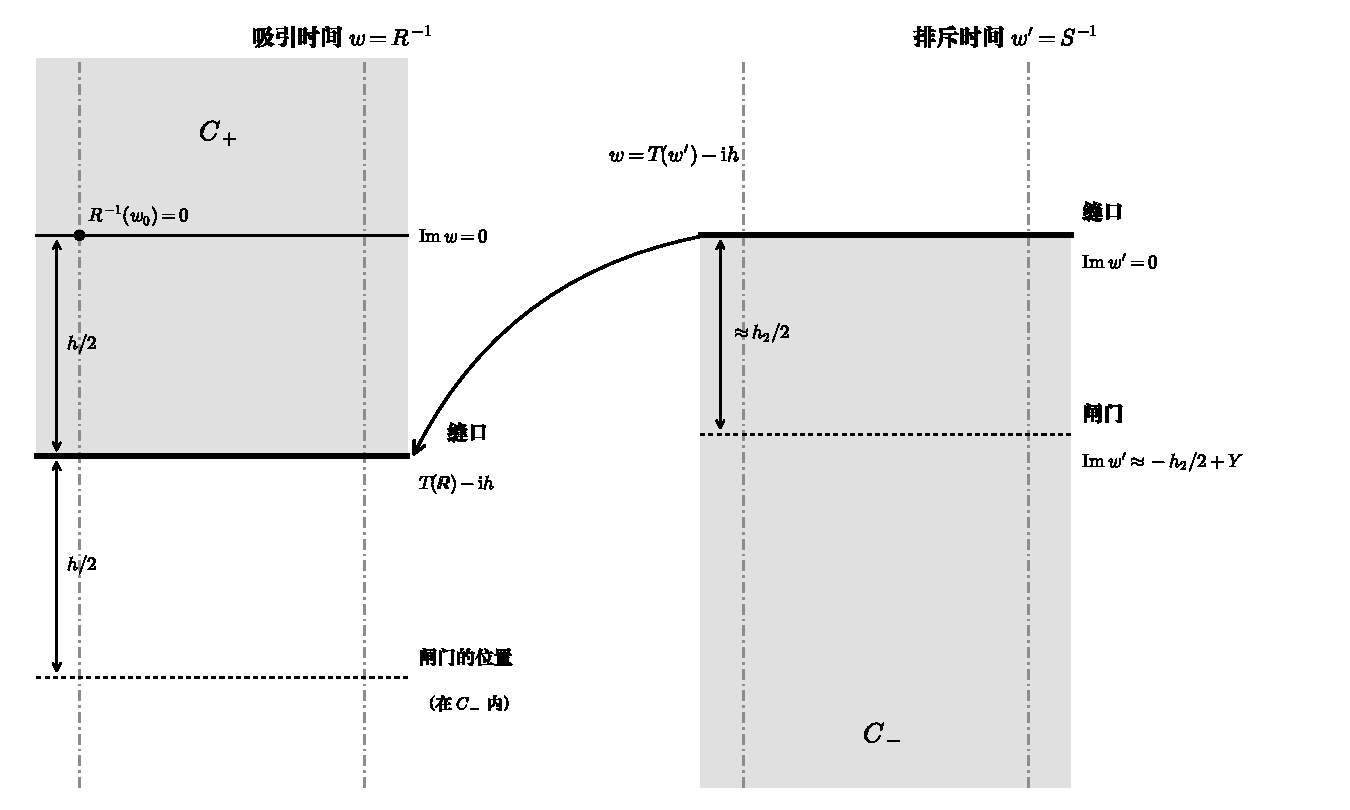
\includegraphics[width=0.8\textwidth]{figures/fig5_cylinders.pdf}
\caption{缝合的两个半柱面（示意图，不按比例；\texttt{figures/fig5\_cylinders.py}）。左：吸引时间 $w=R^{-1}$，
上半柱面 $C_+=\{\Ima w\ge-h/2\}/\Z$。右：排斥时间 $w'=S^{-1}$，下半柱面 $C_-=\{\Ima w'\le0\}/\Z$。
右侧缝口上的点 $w'$ 粘到左侧的 $T(w')-\ii h$。闸门（第~\ref{ch:confluence} 章中 $T$ 收敛到逆 horn 映射的地方）
在排斥时间里位于缝口下方约 $h_2/2$ 处；换到吸引时间，它在缝口下方约 $h/2$、实轴下方约 $h$ 处。}
\label{ch5:fig:cylinders}
\end{figure}

% ======================================================================
\section[算例]{算例：tetration，$b=1.3$}\label{ch5:sec:example}

\begin{example}\label{ch5:exa:b13}
取 tetration（第~\ref{ch:unfolding} 章的 $u$ 坐标，$a_2=\frac12$，$\rho=\frac13$），$b=1.3$，基点 $w_0=1$。脚本 \texttt{figures/ch05\_transition\_example.py}
调用 \texttt{docs/transition\_map.py}：后者只用两个 Schröder 级数（$L$ 与 $L_2$ 处各 40 项）计算 $R^{-1}$ 与 $S$，
在水平线 $\Ima z=-1$ 上取 $32$ 个点做离散 Fourier 变换（30 位运算）。得到（数值）
\begin{gather*}
 \lambda_1=0.385934936554,\quad \lambda_2=2.06141317173,\quad h=6.59938506301,\\
 \Lam=9.8154483\times10^{-19},\quad p=0.6887315094,\\
 t_0=-5.4493869591344+3.2996925315034\,\ii,\\
 t_1=2.79582973902\times10^{-11}-8.30315822559\times10^{-11}\,\ii .
\end{gather*}
可以核对本章的几个结论：
\begin{itemize}
\item $\Ima t_0-h/2\approx-2\times10^{-27}$（数值误差量级），即 \cref{lem:realT} 的分支条件；$|t_{-1}-\overline{t_1}|\approx2\times10^{-24}$。
\item $|t_1|=8.7612271\times10^{-11}$，而 $|\tau_1|\Lam^{1/2}=0.0884320857\times9.9072944\times10^{-10}$
  $=8.76123\times10^{-11}$（\cref{ch5:cor:size}）。
\item 规范化系数与比值：
  \begin{gather*}
   \tau_1=0.0884320857\,\ee^{1.577579614\,\ii},\qquad
   \tau_2=0.01205500797\,\ee^{-1.566107319\,\ii},\\
   \tau_3=0.001447001346\,\ee^{1.50807325\,\ii},\qquad
   t_2/t_1^2=1.541515038\,\ee^{1.561918759\,\ii}.
  \end{gather*}
  对照抛物极限（第~\ref{ch:confluence} 章）：$|B_1|=0.0890584364$，$\arg(B_1\ee^{2\pi\ii a})=1.5865330757$，
  $|B_2|=0.0124873841$，$|B_3|=0.0015927899$，$B_2/B_1^2=1.5744226855\,\ee^{1.5868794187\,\ii}$。
  在 $p\approx0.69$ 处，$|\tau_1|,|\tau_2|,|\tau_3|$ 与极限 $|B_n|$ 的相对差约为 $0.7\%$、$3.5\%$、$9\%$，与 $O(p)$ 的收敛速率（\cref{thm:first-order}）相容。
\end{itemize}
\emph{换基点.} 改用 $w_0'=0.5$（它满足 (H4)）。脚本给出 $\Delta=R^{-1}(0.5)=-0.65860846751381$（实数），
$t_0-t_0'=-0.65860846751381=\Delta$，$t_n'=t_n$（$n\ne0$），$|\tau_n'|=|\tau_n|$ 到所有显示的位数，并且
$\arg\tau_1'=-2.560579432=\arg\tau_1+2\pi\Delta\pmod{2\pi}$（差 $3\times10^{-24}$），与 \cref{prop:base-point} 一致。
$t_2/t_1^2$ 两者相同。

\emph{预言.} 若接受 \eqref{ch5:eq:chat-tau}（第~\ref{ch:sewing} 章证明），则 $b=1.3$ 处缝合解的第一个分离系数是
$c_1\approx\Lam\tau_1\approx8.68\times10^{-20}\,\ee^{1.5776\,\ii}$。在实轴附近，按 \cref{ch5:prop:first-sep}，
缝合解与正则解 $R$ 的差约为 $|c_1R'(x)(\ee^{2\pi\ii x}-1)|\lesssim2\times10^{-19}|R'(x)|$：
在 $b=1.3$，两种``半次迭代''在实轴上的差别在第 19 位小数。
\end{example}

\begin{remark}[在哪条线上取样]\label{ch5:rem:sampling}
\cref{ch5:cor:size} 有一个实际的推论。在实轴上取样时，$t_3$ 的大小是 $|\tau_3|\Lam^{3/2}\approx1.4\times10^{-30}$，
不高于这次计算的数值底（30 位运算，实轴上的舍入误差约 $10^{-30}$），所以在实轴上算出的 $\tau_3$ 毫无意义（脚本给出 $|\tau_3|\approx3.5$）。
在 $\Ima z=-1$ 上取样，第 $n$ 个正模被放大 $\ee^{2\pi n}$ 倍，$\tau_3$ 就能算准。更一般地，
正模应当在全纯带中尽量靠下的线上读出。第~\ref{ch:confluence} 章的闸门正是带的下边缘附近、$T$ 的正模变成 $O(1)$ 的地方。
\end{remark}

\cite{KneserPaper} 的表 tab:tau 把 $\tau_1$、$t_2/t_1^2$ 与从 Kneser 型解直接外推得到的 $\hat c_1$、$\Xi_2$ 作比较：
在 $b=1.10$ 处，$\hat c_1$ 与 $\tau_1$ 的模与辐角都一致到 8 位（数值）。这是 \eqref{ch5:eq:chat-tau} 的数值印证。

\begin{example}[其他族；换基点的数值检验]\label{ch5:exa:families}
\cite{KneserPaper} 的一般化检验（\texttt{docs/generality-check-zh.md} §2，脚本 \texttt{docs/generality\_check.py}，60 位运算）
对第~\ref{ch:unfolding} 章的四个族在 $\lambda_1=0.97$ 处计算了转移映射。下面的数都是数值。
\begin{itemize}
\item 分支条件：四个族的 $|\Ima t_0-h/2|$ 分别不超过 $5\times10^{-57}$、$10^{-43}$、$3\times10^{-31}$、$3\times10^{-59}$，与 \cref{lem:realT} 一致。
\item $|\tau_1|/|B_1|-1$ 分别为 $-9.4\times10^{-6}$、$-1.4\times10^{-5}$、$-1.3\times10^{-5}$、$+1.0\times10^{-3}$；
  $p\approx9\times10^{-4}$，所以偏差是 $O(p)$ 的量级。
\item 二次族取三个基点 $w_0=0$、$0.2$、$0.35$：$|\tau_1|/|B_1|$ 三者都等于 $0.999986451728$，
  而一阶系数 $\log(\tau_1/B_1\ee^{2\pi\ii a})/p$ 的实部三者都等于 $-0.01504809108$（十位一致），虚部分别为 $-0.0748$、$7.788$、$115.8$。
  这正是 \cref{prop:base-point}：模长与实部是不变量，辐角与虚部是基点规范。
\end{itemize}
\end{example}

% ======================================================================
\notes

\textbf{来源.} 本章对应 \cite{KneserPaper} 的 The separation is a transition-map invariant 一节：
\cref{ch5:lem:RS}(3) 与 \cref{lem:realT} 对应 Lemma realT 及其前的定义，\cref{ch5:rem:normalisations} 对应式 (taun) 后的讨论，
\cref{thm:welding} 与 \cref{ch5:cor:cn} 对应 Theorem welding 与 Corollary cn，\cref{ch5:prop:gauge} 对应 Remark invariance。
一般开折的版本（基点条件改为 (H4)）见论文 General real saddle-node unfoldings 一节的改写清单。
\cref{prop:base-point} 与 \cref{cor:invariance} 对应该节的 命题~9.6 与推论~9.7；
这里补全了论文中只写了一句话的共轭不变性证明（Koenigs 坐标的变换、$S$ 的平移、借助辅助基点 $w_0'$）。
\cref{lem:realT}(3) 中的 $T'>0$ 在论文中出现于 Proposition weld-parameter 的证明。
\cref{ch5:lem:strip}(2) 的周期性证明（用实轴上辐角为常数排除 $2\pi\ii k$）是本书补的。

\textbf{双坐标.} 用两个不动点处的 Koenigs 坐标描述一个超越函数的``分数次迭代''，在 tetration 的数值文献中早已出现：
Kouznetsov--Trappmann 在 $b=\sqrt2$ 处比较了四个正则超指数 \cite{KouznetsovTrappmann2010}；
Nixon 用 $F=R\circ(\id+\theta)$ 的形式比较非正则解与正则解 \cite{Nixon2022}，
这正是本章 $K=R\circ(\id+P)$ 的写法。本章的新意在于把两个坐标之间的转移映射 $T$ 作为基本对象，
并证明分离系数是它的函数（焊接恒等式）。

\textbf{与开折模的关系.} 当 $s\to0$ 时，$T$ 收敛到逆 horn 映射（第~\ref{ch:confluence} 章），后者是 Écalle--Voronin 模
\cite{Ecalle1981,Voronin1981}。对固定的 $s>0$，$T$ 是两个双曲不动点的 Koenigs 坐标之间的``Glutsyuk 型''转移映射，
它与 Marde\v{s}i\'c--Roussarie--Rousseau 的开折模 \cite{MRR2004} 的确切关系没有推导。
\cref{cor:invariance} 只说明 $|\tau_n|$ 与 $\Rea\kappa^{(n)}_j$ 是不变量；它们是否构成完全不变量，是开放的。

% ======================================================================
\exercises

\begin{exercise}\label{ch5:ex:period}
证明 $R^{-1}$ 的分支相差 $\ii h\Z$，$S^{-1}$ 的分支相差 $\ii h_2\Z$（在 $\sigma_{\rm rep}$ 的值域内）。
由此说明为什么不存在一个同时等于 $R$ 与 $S$ 的平移的解。
\end{exercise}

\begin{exercise}\label{ch5:ex:mobius}
补全 \cref{ch5:exa:mobius} 的细节：验证 $\sigma$、$\sigma_{\rm rep}$ 的公式与 $\lambda_1\lambda_2=1$，并证明 $S(z)=R(z+t_0)$。
若把基点取在 $(L,L_2)$ 中，$\Ima t_0$ 等于什么？这说明 (H4) 中``基点在 $L$ 远侧''的作用。
\end{exercise}

\begin{exercise}\label{ch5:ex:translations}
直接验证 \cref{ch5:rem:normalisations} 中的三条变换规则，并说明：若 $S$ 换成 $\sigma_{\rm rep}^{-1}(-c\lambda_2^z)$（$c>0$），
则 $\tau_n$ 不变。若 $c<0$ 呢？
\end{exercise}

\begin{exercise}\label{ch5:ex:conj}
设 $s$ 为实数。证明 $\overline{T(\bar z)}=T(z)-\ii h$（在 $\Ima t_0=h/2$ 的分支上），并由此再证一次 $t_{-n}=\overline{t_n}$。
\end{exercise}

\begin{exercise}\label{ch5:ex:real-K}
设 $K$ 是双侧解，实轴含于 $U_+$，并且 $K$ 在实轴上取实值。证明 $P$ 是常数，从而 $K$ 是 $R$ 的平移。
由此说明：$c_1\ne0$ 的双侧解在实轴上不可能是实值的。
\end{exercise}
\begin{hint}
对实的 $x$，$K(x)$ 在 $\mathcal A(L)$ 中的实点，$\Ima R^{-1}(K(x))\in\frac h2\Z$。所以 $\Ima P$ 在实轴上是常数；
一个只有非负模的周期函数，若虚部在实轴上为常数，则它是常数。
\end{hint}

\begin{exercise}\label{ch5:ex:welding-trivial}
设 $\varphi_-=\id-g_0$（即 $G\equiv g_0$）。证明 \eqref{ch5:eq:welding} 化为 $t_n=c_n\ee^{2\pi\ii ng_0}$，并解释：
此时 $T=\varphi_+\circ(\id+g_0)$ 只有非负模，而由 \cref{lem:realT}(2)，这只能在 $T$ 是平移时发生。
\end{exercise}

\begin{exercise}\label{ch5:ex:negative}
仿照 \cref{thm:welding} 的证明，导出负模的公式 $t_{-n}=[G]_{-n}+\sum_{m\ge0}c_m[\ee^{2\pi\ii mG}]_{-n-m}$（$n\ge1$）。
\end{exercise}

\begin{exercise}\label{ch5:ex:first-two}
写出 \eqref{ch5:eq:welding} 在 $n=1,2$ 时的前两项。设 $|c_m|\le C\Lam^m$，并且在 $\Ima w=-Y$ 上 $|G-g_0|\le\epsilon$。
用 $[F]_k$ 在不同高度上计算的自由，估计 $|[\ee^{2\pi\ii mG}]_{-k}|$，并说明在什么条件下 $t_1\ee^{-2\pi\ii g_0}=c_1(1+O(\Lam))$。
\end{exercise}
\begin{hint}
$[F]_{-k}=\int_0^1F(x-\ii Y)\ee^{2\pi\ii k(x-\ii Y)}\dd x$，其模不超过 $\sup|F|\,\ee^{2\pi kY}$；$Y$ 应取得尽量小，即尽量靠近缝口。
\end{hint}

\begin{exercise}\label{ch5:ex:gauge}
设 $K$ 是双侧解，$K(0)=w_0$。对复数 $\delta$，$K(\cdot+\delta)$ 的值 $K(\delta)$ 一般不是实数。说明为什么
$|c_1|$ 的``物理意义''需要基点是实数，并验证 \cref{prop:base-point}(3)。
\end{exercise}

\begin{exercise}\label{ch5:ex:numerics}
运行 \texttt{figures/ch05\_transition\_example.py}，把取样线改为 $\Ima z=0$ 与 $\Ima z=-2$，比较 $\tau_1,\tau_2,\tau_3$。
在 $b=1.3$ 处，$T$ 的全纯带大约有多宽？用 \cref{ch5:cor:size} 解释你看到的现象。
\end{exercise}

\begin{exercise}\label{ch5:ex:invariance-quad}
设 $A(w)=\alpha w+\beta$，$\alpha>0$，$\tilde f_s=A\circ f_s\circ A^{-1}$，$\tilde w_0=A(w_0)$。
不经 \cref{cor:invariance}，直接证明 $\tilde R=A\circ R$、$\tilde S=A\circ S(\cdot-c')$（求出 $c'$），从而 $\tilde\tau_n=\tau_n$（不只是模相等）。
$\alpha<0$ 时会发生什么？
\end{exercise}
\begin{hint}
$\alpha<0$ 时 $a_2$ 变号，需要先用 第~\ref{ch:unfolding} 章的符号约定翻转；上下半平面互换，逆上 horn 映射换成逆下 horn 映射。
\end{hint}

% 第 6 章 缝合解
% 来源：[KneserPaper] §3.3（Welding construction）、§6（W2）、§7（W1）、§8（char）、Remark paulsen；
%       sec-general.tex 的改写清单；docs/theory-core-zh.md §2；docs/quad-kneser-zh.md §4。
% 本章新宏（\providecommand，名字带特征前缀以免与他章冲突）：
\providecommand{\WienerA}{\mathfrak A}          % 加权 Wiener 代数 𝔄_H
\providecommand{\Tcirc}{T^{\circ}}               % T° = T − id − t₀
\providecommand{\Pineg}{\Pi_{<0}}                % 负模投影
\providecommand{\Pinonneg}{\Pi_{\ge 0}}          % 非负模投影
\providecommand{\Csew}{\mathcal C}               % 类 𝒞(Y)
\providecommand{\etwopi}[1]{\ee^{2\pi\ii #1}}    % e^{2πi·}
\providecommand{\Rtime}{\mathcal R}              % 吸引时间（R⁻¹ 的一个分支）
\providecommand{\Stime}{\mathcal S}              % 排斥时间（S⁻¹ 的一个分支）
\providecommand{\Band}{\mathcal B}               % 带状透镜 𝓑_s(Y)

\chapter{缝合解}\label{ch:sewing}

前两章给出了两个吸引、排斥正则解 $R,S$ 和它们之间的转移映射 $T=R^{-1}\circ S$。
任何一个「上方用 $R$ 表示、下方用 $S$ 表示」的分数迭代，其分离系数都由 $T$ 决定（\cref{thm:welding}）。
但到目前为止，我们还不知道这样的分数迭代是否存在，也不知道它是否唯一。

本章回答这两个问题。构造是几何的：把 $R$ 的上半柱面和 $S$ 的下半柱面沿 $T-\ii h$ 共形缝合，
缝出的曲面同构于 $\C^*$，它的万有覆叠坐标给出一个分数迭代 $\Ksew$，称为\textbf{缝合解}（sewing solution）。
为了得到定量信息，我们再用加权 Wiener 代数中的一个压缩映射把同一个解构造一遍。
压缩给出 $c_n/\Lam^n-\tau_n=O(\Lam)$，常数只依赖于族。
最后我们证明：在「缝口高度条件」规定的类中，缝合解是唯一的；这个条件是一个选根条件，不能去掉。

\begin{goals}
\item 两个半柱面沿 $T-\ii h$ 的共形焊接给出 $\C^*$，从而给出缝合解 $\Ksew$（\cref{ch6:prop:weld}）。
\item 加权 Wiener 代数 $\WienerA_H$ 中的压缩 $\mathcal T(Q)=-\Pineg[\Tcirc\circ(\id+Q)]$ 构造 $\Ksew$，
  并给出 $|c_n/\Lam^n-\tau_n|\le C_n\Lam$（\cref{thm:sewing}）。
\item $\Ksew$ 对开折参数全纯依赖；$\Ima s<0$ 时它在 $\pm\ii\infty$ 分别趋于两个不动点（\cref{ch6:thm:parameter}）。
\item 类 $\Csew(Y)$ 与刻画定理：$\Csew(Y)=\{\Ksew\}$（\cref{def:class,thm:characterization}）；
  缝口高度条件排除了平移解 $\Ksew(\cdot+c_j)$。
\item 一阶修正：在 (H5) 下 $\hat c_1/\tau_1-1=\Lam[-4\pi^2|\tau_1|^2-2\pi\ii\tau_1-4\pi\ii\tau_2\bar\tau_1/\tau_1]+O(\Lam^2)$，
  以及它的数值检验（\cref{ch6:prop:first-correction}）。
\end{goals}

\section{设定与回顾}\label{ch6:sec:setup}

本章始终在下面的设定中工作。

\paragraph{族与尺度.}
$f_s$ 是满足 (H1)--(H4) 的实鞍结开折（\cref{def:unfolding}），$s>0$ 一侧有两个实不动点。
$u$ 是仿射坐标 $w=w^*+cu$；为了书写简单，本章取 $c=1$，即 $u=w-w^*$
（对 tetration 取 $c=\ee$ 时只需把下文的 $w^*+u_j$ 换成 $w^*+\ee u_j$，估计不变）。在 $u$ 坐标下仍把映射写成 $f_s$。吸引、排斥不动点为 $u_1<u_2$，乘子 $0<\lambda_1<1<\lambda_2$，
留数 $A_j=1/\log\lambda_j$，周期 $h=2\pi/|\log\lambda_1|$、$h_2=2\pi/\log\lambda_2$，强迫尺度 $\Lam=\ee^{-2\pi h}$。
由 \cref{prop:scales} 与 \cref{lem:residues}，当 $s\to0^+$ 时
\begin{gather}\label{ch6:eq:scales}
 |\log\lambda_1|,\ \log\lambda_2=2\sqrt{a_2\gamma s}\,\bigl(1+O(\sqrt s)\bigr),\\
 A_1+A_2\to\rho,\qquad A_1(u_1-u_2)\to\frac1{a_2},\qquad h_2-h\to2\pi\rho .\notag
\end{gather}
特别地 $h\to\infty$，$\Lam\to0$，并且 $|u_1|,|u_2|\le C|\log\lambda_1|$。
本章所有「常数」都只依赖于族（即依赖于 $f_s(w)$ 在 $(s,w)=(0,w^*)$ 附近的芽和基点 $w_0$），不依赖于 $s$；
$C$ 表示这样的常数，每次出现可以不同。

\paragraph{两个正则解与转移映射.}
吸引正则解 $R(z)=\sigma^{-1}(\sigma(w_0)\lambda_1^{z})$（\cref{def:regular-solution}），$R(0)=w_0$，
以 $\ii h$ 为周期（因为 $\lambda_1^{\ii h}=\ee^{\ii h\log\lambda_1}=\ee^{-2\pi\ii}=1$）。它满足
\begin{equation}\label{ch6:eq:sigmaR}
 \sigma\bigl(R(w)\bigr)=\sigma(w_0)\,\lambda_1^{w},
\end{equation}
只要左边有定义。$R$ 不是整函数：$\sigma^{-1}$ 只能沿 $f_s$ 的逆分支延拓，$R$ 在一个闭集 $\Sigma_R$ 外全纯，
$\Sigma_R$ 由 $f_s$ 的奇异值经逆分支拉回得到（对 tetration，$\Sigma_R=\bigcup_k((-\infty,-2]+\ii kh)$）。
排斥正则解 $S(z)=\sigma_{\mathrm{rep}}^{-1}(-\lambda_2^{z})$ 由 (H1) 延拓为整函数，以 $\ii h_2$ 为周期，
把 $\R$ 递减地映到 $(w^*+u_1,w^*+u_2)$ 上（\cref{def:transition}）。

转移映射 $T=R^{-1}\circ S$ 取 \cref{lem:realT} 的分支：$\Ima t_0=h/2$。于是
\begin{equation}\label{ch6:eq:Treal}
 T(z)-z=\sum_{n\in\Z}t_n\etwopi{nz},\qquad T(x)-x-\tfrac{\ii h}2\in\R\ (x\in\R),\qquad t_{-n}=\overline{t_n},
\end{equation}
$\tau_n=t_n\etwopi{(-nt_0)}$，$\Tcirc=T-\id-t_0$。因为 $|\etwopi{t_0}|=\ee^{-2\pi\Ima t_0}=\ee^{-\pi h}=\Lam^{1/2}$，
\begin{equation}\label{ch6:eq:tn-size}
 |t_n|=|\tau_n|\,\Lam^{n/2}\qquad(n\ge1).
\end{equation}
所以只要 $\tau_n$ 有界（第 7 章证明它们收敛），$T$ 的非零模就是指数小的。
本章不用第 7 章的收敛结果；我们直接从带状区域上的估计得到 $t_n$ 的一致上界（\cref{ch6:lem:modes}）。

\paragraph{解与分离系数.}
\textbf{解}（solution）指一个在某闭集（\textbf{奇异集}，singular set）之外全纯、并在有定义处满足
\begin{equation}\label{ch6:eq:abel}
 K(z+1)=f_s\bigl(K(z)\bigr)
\end{equation}
的函数（这里 $f_s$ 写在 $w$ 坐标下）。若 $K=R\circ(\id+P)$ 在一个上半平面上成立，其中 $P$ 是有界、全纯、$1$-周期的，
那么在 $q=\etwopi{z}$ 下 $P$ 是穿孔圆盘上的有界全纯函数，$q=0$ 是可去奇点，所以
\begin{equation}\label{ch6:eq:P-expansion}
 P(z)=\sum_{n\ge0}c_n\etwopi{nz},\qquad P(z)\to c_0\quad(\Ima z\to+\infty).
\end{equation}
$c_n$ 是\textbf{分离系数}（separation coefficients），$\hat c_n=c_n/\Lam^n$，$\Xi_n=c_n/c_1^n$。同理，下半平面上有界周期的 $Q$ 只有非正模。
这个「有界周期函数只有单侧模」的事实本章会反复使用。

\section{共形焊接}\label{ch6:sec:weld}

\subsection{缝合曲面}

\begin{proposition}[焊接]\label{ch6:prop:weld}
设 $s>0$ 足够小。取两个半柱面
\[
 C_-=\{\Ima w'\le0\}/\Z\quad(\text{排斥时间}),\qquad
 C_+=\{\Ima w\ge-h/2\}/\Z\quad(\text{吸引时间}),
\]
把 $C_-$ 的边界与 $C_+$ 的边界按 $w=T(w')-\ii h$ 等同。
\begin{enumerate}
\item 得到的曲面 $X$ 是一个 Riemann 曲面，且 $X\cong\C^*$。
\item 设 $z$ 是 $X$ 的万有覆叠坐标，选成使覆叠变换为 $z\mapsto z+1$、且上端对应 $\Ima z\to+\infty$。那么
 \[
  K(z)=R\bigl(w(z)\bigr)\ \ (\text{$z$ 在 $C_+$ 的提升中}),\qquad K(z)=S\bigl(w'(z)\bigr)\ \ (\text{$z$ 在 $C_-$ 的提升中})
 \]
 是 \eqref{ch6:eq:abel} 的解，在 $w(z)\in\Sigma_R$ 的点之外全纯。
\item $w(z)-z$ 是 $1$-周期的，在上端附近只有非负模；$w'(z)-z$ 是 $1$-周期的，在下端附近只有非正模。
 坐标 $z$ 在相差一个平移的意义下唯一。
\end{enumerate}
\end{proposition}

\begin{proof}
(1) 由 \eqref{ch6:eq:Treal}，$T(x)-\ii h$ 的虚部恒为 $-h/2$，所以 $T-\ii h$ 把 $C_-$ 的边界圆 $\R/\Z$ 映到 $C_+$ 的边界圆
$(\R-\ii h/2)/\Z$。由 \cref{lem:realT}(3)，$T(x+1)=T(x)+1$，$T'(x)>0$，并且 $T-\ii h$ 把 $\R$ 双射地映到 $\R-\ii h/2$
（$T'>0$ 的来源是：$S'<0$，而 $(R^{-1})'=\sigma'/(\sigma\log\lambda_1)$ 在线段 $(w^*+u_1,w^*+u_2)$ 上也为负）。
所以粘合映射是边界圆之间保向的实解析微分同胚，并延拓为边界附近的全纯映射。
在边界的一个邻域内用这个全纯延拓作为坐标变换，$X$ 就有了复结构。

$X$ 在拓扑上是一个开柱面。它的两端是穿孔圆盘：上端用坐标 $\etwopi{w}$（$\Ima w\to+\infty$），下端用 $\etwopi{(-w')}$。
补上两个点后得到单连通的紧 Riemann 曲面，由单值化定理它是 $\widehat\C$。去掉两点，$X\cong\C^*$。

(2) 在缝上两个定义一致：$R(T(w')-\ii h)=R(T(w'))=S(w')$，因为 $\ii h$ 是 $R$ 的周期，并且 $R\circ T=S$。
$\pi_1(X)\cong\Z$ 的生成元提升为 $z\mapsto z+1$，在两个图上分别作用为 $w\mapsto w+1$、$w'\mapsto w'+1$，
所以 $K(z+1)=R(w+1)=f_s(R(w))=f_s(K(z))$，下方同理（$S(w'+1)=f_s(S(w'))$）。

(3) 在上端附近，$q=\etwopi{z}$ 与 $\etwopi{w}$ 都是 $X$ 的穿孔圆盘坐标，并且都在该端趋于 $0$；
它们之间的坐标变换是穿孔圆盘之间的双全纯映射，把穿孔映到穿孔，因此是在 $0$ 处有单零点的全纯函数：
$\etwopi{w}=q\,\exp(\text{$q$ 的全纯函数})$。取对数即知 $w-z$ 是 $q$ 的全纯函数，只有非负模。下端同理。
$\C^*$ 的保持两端的自同构是 $q\mapsto\alpha q$，所以 $z$ 唯一到相差平移。
\end{proof}

\begin{definition}[缝合解]\label{ch6:def:sewn}
在 \cref{ch6:prop:weld} 中，$0\in\C$ 落在 $C_+$ 内部（因为 $0>-h/2$）。
选坐标 $z$ 使 $z=0$ 对应 $C_+$ 中的点 $w=0$，并且 $w(z)=z+P(z)$，$P$ 有界周期、$P(0)=0$。
所得的解记为 $\Ksew=\Ksew_s$，称为\textbf{缝合解}。它满足 $\Ksew(0)=R(0)=w_0$。
\end{definition}

\begin{remark}\label{ch6:rem:normalisation}
「$\Ksew(0)=w_0$」本身并不确定平移：$C_+$ 中的点 $w=\ii jh$（$j\ge1$）也被 $R$ 映到 $w_0$。
\cref{ch6:def:sewn} 用的是更细的归一化：标记点是 $C_+$ 中的 $w=0$ 这一个点。
\cref{ch6:sec:char} 会说明：选错标记点得到的平移解 $\Ksew(\cdot+c_j)$ 正是缝口高度条件要排除的东西。
\end{remark}

\begin{remark}[奇异集]\label{ch6:rem:singular}
$S$ 是整函数，而 $R$ 不是，所以 $\Ksew$ 的奇异集全部来自上方的 $R$ 表示：它是 $w^{-1}(\Sigma_R)$。
对 tetration，除了 $(-\infty,-2]$ 附近的割线，还有 $(-\infty,-2]+\ii kh$（$k\ge1$）附近的副本落在 $R$ 表示的区域里。
\end{remark}

由 \cref{ch6:prop:weld}(3)，$\Ksew$ 满足 \cref{thm:welding} 的假设（上方 $\varphi_+=w$，下方 $\varphi_-=w'$），
所以它的分离系数由焊接恒等式与 $T$ 的 Fourier 系数相联系。\Cref{ch6:sec:contraction} 把这个联系定量化。

\begin{figure}[htbp]
\centering
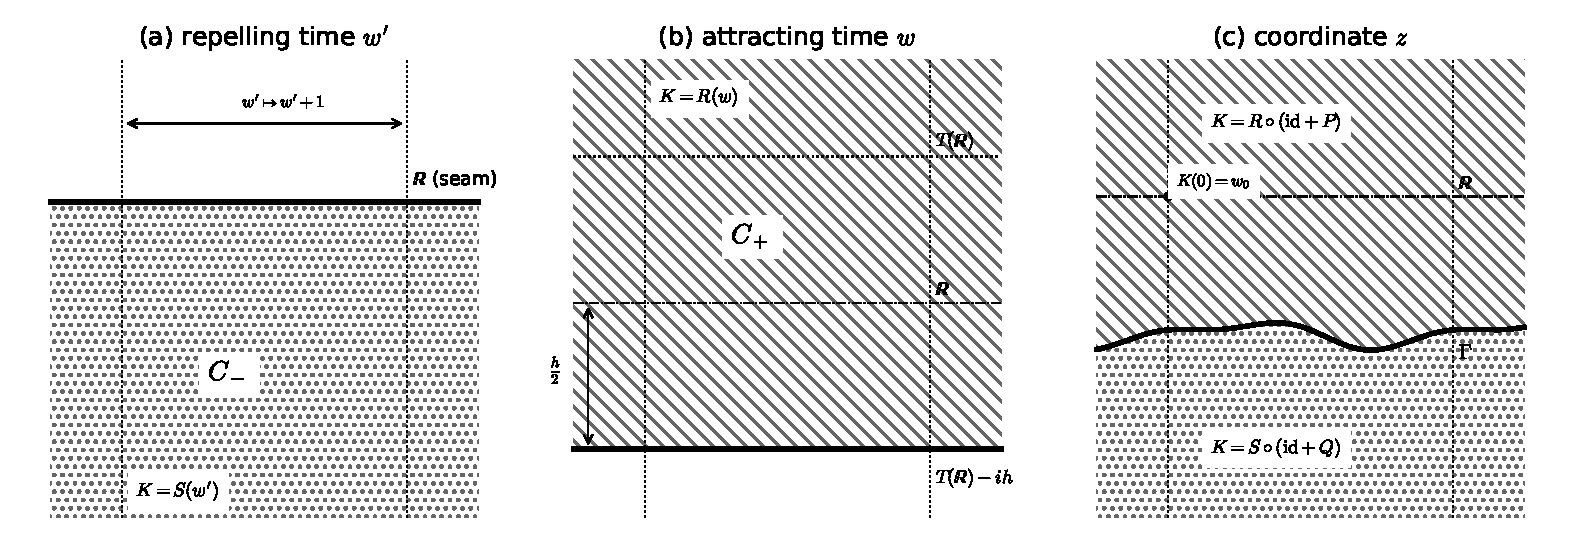
\includegraphics[width=\textwidth]{figures/fig6_welding.pdf}
\caption{缝合解的焊接示意（脚本 \texttt{figures/fig6\_welding.py}）。(a) 排斥时间 $w'$ 中的下半柱面 $C_-$，缝是实轴；
(b) 吸引时间 $w$ 中的上半柱面 $C_+$，缝是直线 $\Ima w=-h/2$，它是 $\R$ 在 $T-\ii h$ 下的像；
点线 $T(\R)$ 在实轴上方半个周期处。(c) 单值化坐标 $z$：缝 $\Gamma$ 是 $\Ima z\approx-h/2$ 附近的一条曲线，
上方 $K=R\circ(\id+P)$，下方 $K=S\circ(\id+Q)$，$K(0)=w_0$。虚线是基本域的边界。}
\label{ch6:fig:welding}
\end{figure}

\subsection{参数依赖：Fischer--Grauert 论证}

缝合解是用单值化定义的，单值化映射对参数的依赖并不自动全纯。下面的论证对每个固定的 $s_0$ 都成立，但不给出一致的估计。

\begin{proposition}[缝合族的局部参数依赖]\label{ch6:prop:weld-family}
设 $s_0>0$ 足够小。则存在复圆盘 $\Delta\ni s_0$，使 \cref{ch6:def:sewn} 的缝合解延拓为 $\Delta$ 上的全纯族：
在万有覆叠坐标的每个公共正则区域上，$\Ksew_s(z)$ 对 $(s,z)$ 联合全纯，$\Ksew_s(0)=w_0$。
不同 $s_0$ 的局部族在重叠处一致，因而定义在 $(0,s_1)$ 的一个复邻域上（这里不断言邻域的宽度一致）。
\end{proposition}

\begin{proof}
两个不动点及其 Koenigs 坐标在 $s_0$ 附近全纯依赖于 $s$。紧集 $S_{s_0}([0,1])\subset(w^*+u_1,w^*+u_2)$ 在吸引域内且不含不动点，
所以所选的 $T_s=R_s^{-1}\circ S_s$ 的分支在「参数圆盘 $\times$ $[0,1]$ 附近的窄带」上联合全纯；
$T_s(w'+1)=T_s(w')+1$ 把它延拓到整条带。\Cref{ch6:prop:weld} 的证明说明 $T_{s_0}'>0$ 在 $\R$ 上成立。
由紧性与局部单射性，存在更窄的带使 $T_{s_0}$ 在其上模 $1$ 单射；缩小参数圆盘后这一性质保持，
并且实圆周的像是柱面中的解析 Jordan 曲线。

令 $U_s=T_s+\varpi_s$，$\varpi_s=2\pi\ii/\log\lambda_1(s)$ 是 $R_s$ 的周期；在实的 $s$ 处 $\varpi_s=-\ii h$，$U_s=T_s-\ii h$。
取小的 $\delta>0$，排斥图 $\{\Ima w'<\delta/2\}/\Z$ 和吸引图「曲线 $U_s(\{\Ima w'=-\delta/2\})$ 上方」的区域，
在 $|\Ima w'|<\delta/2$ 上用 $(s,w')\mapsto(s,U_s(w'))$ 等同。缩小参数圆盘后，这些图与坐标变换构成一个 Hausdorff 的全纯柱面族；
在 $s=s_0$ 处它就是 \cref{ch6:prop:weld} 的焊接（用解析领口代替边界）。用与参数无关的局部坐标 $\etwopi{w}$、$\etwopi{(-w')}$ 补上两端，
得到一个真的全纯淹没，纤维是亏格 $0$ 的紧 Riemann 曲面。两个补上的点与上图中的点 $w=0$ 是三个互不相交的全纯截面
（缩小圆盘后 $w=0$ 留在缝的上方）。

纤维两两双全纯的真全纯族是局部全纯平凡的（Fischer--Grauert 定理~\cite{FischerGrauert1965}）。
再用逐纤维的唯一 Möbius 变换把三个截面送到 $0,\infty,1$，得到在紧化纤维上联合全纯的坐标 $q_s$。
取局部提升 $z=(2\pi\ii)^{-1}\log q_s$，使标记点 $w=0$ 对应 $z=0$。在重叠区的提升上，$R_s(U_s(w'))=S_s(w')$，
因为 $\varpi_s$ 是 $R_s$ 的周期。所以两个正则解定义了 $\Ksew_s$，它在两个表示正则处联合全纯，且 $\Ksew_s(0)=R_s(0)=w_0$。
在实参数上这正是 \cref{ch6:def:sewn} 的焊接。标记坐标使局部族唯一，由恒等定理它们在重叠圆盘上拼接。
\end{proof}

\Cref{ch6:thm:parameter} 会在 $s\to0^+$ 的一侧给出定量的版本：压缩的常数与 $s_0$ 无关，但参数圆盘的大小仍不作一致的断言。

\section{带状区域与转移映射的模}\label{ch6:sec:band}

为了把焊接写成一个压缩问题，需要知道 $T$ 在多宽的带上全纯、以及 $\Tcirc$ 在带上有多小。
本节的估计只用到第 4 章的尺度，不用第 7 章的汇流定理。

\subsection{模型时间与一步误差}

由 Weierstrass 预备定理（\cref{thm:weierstrass-prep}），存在固定的 $r>0$，使 $s$ 小时
\begin{equation}\label{ch6:eq:prepared}
 f_s(u)-u=(u-u_1)(u-u_2)\,k_s(u)\qquad(|u|<r),
\end{equation}
$k_s$ 在 $D_r$ 上全纯、无零点，并一致收敛到 $k_0(u)=(g(u)-u)/u^2=a_2+a_3u+\cdots$。定义\textbf{模型时间}（model time）与两个辅助函数
\[
 \Psi_s(u)=A_1\log(u-u_1)+A_2\log(u-u_2),\qquad
 F_s=\Psi_s\circ f_s-\Psi_s-1,\qquad
 Z_s(u)=A_1\log\frac{u-u_1}{u-u_2}.
\]
$\Psi_s$ 是一个向量场的时间函数，它的时间 $1$ 映射在 $u_1,u_2$ 处的乘子正是 $\lambda_1,\lambda_2$；$F_s$ 衡量 $f_s$ 偏离这个时间 $1$ 映射的程度。

\begin{lemma}[一步误差]\label{ch6:lem:model}
存在 $r'\in(0,r)$ 与常数 $M_1$，使 $s$ 小时：
\begin{enumerate}
\item $F_s$ 在 $D_{r'}$ 上单值全纯，且 $|F_s(u)|\le M_1|u-u_1|\,|u-u_2|$（$u\in D_{r'/2}$）；
\item $Z_s\circ f_s-Z_s$ 在 $D_{r'}$ 上单值全纯，且 $Z_s(f_s(u))-Z_s(u)=1+O(|u|+|\log\lambda_1|)$ 在 $D_{r'/2}$ 上一致成立。
\end{enumerate}
\end{lemma}

\begin{proof}
由 \eqref{ch6:eq:prepared}，$(f(u)-u_1)/(u-u_1)=1+(u-u_2)k(u)$，$(f(u)-u_2)/(u-u_2)=1+(u-u_1)k(u)$，所以
\[
 F=A_1\log\frac{1+(u-u_2)k}{1+(u-u_1)k}+(A_1+A_2)\log\bigl(1+(u-u_1)k\bigr)-1 ,
\]
$r'$ 小时对数的自变量接近 $1$，取主支，$F$ 单值全纯。第一个对数是 $O(|u_1-u_2|)$，而 $A_1(u_1-u_2)$ 与 $A_1+A_2$ 有界（\eqref{ch6:eq:scales}），
所以在 $|u|=r'$ 上 $|F|\le M_0$，$M_0$ 不依赖于 $s$。在 $u=u_1$ 处第一项是 $A_1\log\lambda_1=1$，第二项为 $0$，故 $F(u_1)=0$；
在 $u=u_2$ 处 $F(u_2)=-A_1\log\lambda_2+(A_1+A_2)\log\lambda_2-1=A_2\log\lambda_2-1=0$。
于是 $F/((u-u_1)(u-u_2))$ 在 $D_{r'}$ 上全纯，由最大模原理，它在 $D_{r'}$ 上不超过 $M_0/(r'/2)^2$（当 $|u_j|<r'/2$）。取 $M_1=4M_0/r'^2$。

(2) $Z(f(u))-Z(u)=A_1[\log(1+(u-u_2)k)-\log(1+(u-u_1)k)]=A_1(u_1-u_2)k(u)\,(1+O(|u|+|u_1|+|u_2|))$。
又 $\lambda_1=1+(u_1-u_2)k(u_1)$ 给出 $A_1(u_1-u_2)=1/k(u_1)+O(|u_1-u_2|)$，而 $k(u)/k(u_1)=1+O(|u-u_1|)$。
再用 $|u_j|\le C|\log\lambda_1|$。
\end{proof}

\begin{remark}
第 7 章的汇流定理用的是同样的两个估计（见 \cref{lem:petal}）：沿吸引轨道 $\Ima Z$ 基本不动、$\Rea Z$ 每步增加约 $1$，
而 $\sum_k|F(f^ku)|$ 一致可和。这里我们把它们用在一个不同的区域上：两个不动点之间的「透镜」。
\end{remark}

\subsection{透镜}

在 $\C\setminus((-\infty,u_1]\cup[u_2,\infty))$ 上取 $Z_s$ 的分支使 $\Ima Z_s\in(0,h)$。
在线段 $(u_1,u_2)$ 上 $(u-u_1)/(u-u_2)<0$，这一分支给出 $\Ima Z_s=h/2$；在 $\Ima u>0$ 上 $\Ima Z_s<h/2$。对 $Y>0$ 令
\[
 \Band_s(Y)=\{u:\ Y<\Ima Z_s(u)<h-Y\},
\]
它是以 $u_1,u_2$ 为角点、由两条圆弧围成的透镜，包含线段 $(u_1,u_2)$。记
\[
 c_\rho:=\pi|\rho|+1 .
\]

\begin{lemma}[透镜]\label{ch6:lem:band}
存在常数 $Y_B\ge8$，使对 $Y_B\le Y\le h/2$ 与所有足够小的 $s>0$：
\begin{enumerate}
\item 每个 $u\in\Band_s(Y)$ 的前向轨道留在 $D_{r'}$ 中并趋于 $u_1$，主后向轨道留在 $D_{r'}$ 中并趋于 $u_2$，且
 \[
  \sum_{k\in\Z}|F_s(f_s^ku)|\le\frac CY+C|\log\lambda_1| ;
 \]
\item 吸引时间与实归一化排斥时间
 \[
  \Rtime_s=\Psi_s+\sum_{k\ge0}F_s\circ f_s^k+c_R,\qquad \Stime_s=\Psi_s-\sum_{k\ge1}F_s\circ f_s^{-k}+c_S
 \]
 在 $\Band_s(Y)$ 上全纯且单射。适当选取常数 $c_R,c_S$ 后，$\Rtime_s$ 是 $R^{-1}$ 的分支（与 \cref{lem:realT} 所选分支一致），
 $\Stime_s$ 是 $S^{-1}$ 的分支，在 $(u_1,u_2)$ 上取实值，并且
 \begin{equation}\label{ch6:eq:ImS}
  \bigl|\Ima\Stime_s(u)-(\Ima Z_s(u)-h/2)\bigr|\le\pi|\rho|+\frac CY+C|\log\lambda_1|+o(1)\qquad(s\to0^+);
 \end{equation}
\item $S$ 把带 $\Sigma=\{|\Ima w'|<h/2-Y-c_\rho\}$ 映入 $\Band_s(Y)$，且 $\Stime_s\circ S=\id$。因此 $T=\Rtime_s\circ S$ 在 $\Sigma$ 上全纯，且
 \begin{equation}\label{ch6:eq:Tsum}
  T(w')-w'=(c_R-c_S)+\sum_{k\in\Z}F_s\bigl(f_s^k(S(w'))\bigr).
 \end{equation}
\end{enumerate}
\end{lemma}

\begin{proof}
(i) 令 $q=(u-u_1)/(u-u_2)=\ee^{Z/A_1}$，$\zeta=Z/A_1=-|\log\lambda_1|Z$。在透镜上 $\Ima\zeta\in(-2\pi+|\log\lambda_1|Y,\,-|\log\lambda_1|Y)$。
在 $-2\pi\le\Ima\zeta\le0$ 上，$\ee^\zeta-1$ 只有零点 $0$ 和 $-2\pi\ii$，并有初等不等式
$|\ee^\zeta-1|\ge c\min(1,\delta(\zeta))\max(1,|\ee^\zeta|)$，其中 $\delta(\zeta)=\min(|\zeta|,|\zeta+2\pi\ii|)$，$c>0$ 是绝对常数。
在透镜上 $\delta(\zeta)=|\log\lambda_1|\min(|Z|,|Z-\ii h|)>|\log\lambda_1|Y$。由 $u-u_2=(u_2-u_1)/(q-1)$ 和 $|u_2-u_1|\le C|\log\lambda_1|$ 得
\begin{gather}\label{ch6:eq:bandsize}
 |u-u_2|\le C\Bigl(|\log\lambda_1|+\frac1Y\Bigr),\\
 |u-u_1||u-u_2|=\frac{|q|\,|u_2-u_1|^2}{|q-1|^2}\le
 \begin{cases}C\min(|Z|,|Z-\ii h|)^{-2},&\delta(\zeta)\le1,\\[2pt]
 C|\log\lambda_1|^2\,\ee^{-|\log\lambda_1|\,|\Rea Z|},&\delta(\zeta)>1,\end{cases}
\end{gather}
这里用了 $|q|/\max(1,|q|)^2=\ee^{-|\Rea\zeta|}$。所以 $Y$ 大、$s$ 小时 $\Band_s(Y)\subset D_{r'/2}$。
由 \cref{ch6:lem:model}(2)，只要轨道留在 $D_{r'/2}$ 中，$\Rea Z$ 每步至少增加 $\tfrac34$。

虚部通过 $\Psi_s=Z_s+(A_1+A_2)\log(u-u_2)$ 控制：$\Psi_s(f(u))=\Psi_s(u)+1+F_s(u)$。
沿轨道 $u_k=f^ku$ 有 $\Rea Z(u_k)\ge\Rea Z(u_0)+\tfrac34k$，代入 \eqref{ch6:eq:bandsize}：
$\delta(\zeta_k)\le1$ 的点贡献至多 $C\sum_k(x_k^2+Y^2)^{-1}\le C/Y$（$x_k=\Rea Z(u_k)$ 的间距至少 $\tfrac34$，而 $\min(|Z|,|Z-\ii h|)^2\ge x^2+Y^2$），
其余的点贡献至多 $C|\log\lambda_1|^2\sum_k\ee^{-|\log\lambda_1||x_k|}\le C|\log\lambda_1|$。由 \cref{ch6:lem:model}(1)，$\sum_k|F(u_k)|\le C/Y+C|\log\lambda_1|$。
另一方面 $\Ima Z-\Ima\Psi=-(A_1+A_2)\arg(u-u_2)$，$\arg(u-u_2)\in(0,2\pi)$ 在透镜上成立。所以沿轨道 $\Ima Z$ 的漂移至多
$C/Y+C|\log\lambda_1|+2\pi|A_1+A_2|$。取 $Y_B\ge\max(8,\,8\pi|\rho|+8,\,C)$，则 $s$ 小时它小于 $1+1+2\pi|\rho|+1<Y/2$。
归纳可知轨道留在 $\Band_s(Y/2)\subset D_{r'/2}$ 中，$\Rea Z(u_k)\to+\infty$，即 $u_k\to u_1$；
沿轨道延拓的 $Z$ 值虚部在 $(Y/2,h-Y/2)\subset(0,h)$ 中，所以与固定的割平面分支一致。

后向轨道是\textbf{反射逆族}（reflected inverse family）$G_s(v)=-f_s^{-1}(-v)$ 的前向轨道。它在 $(0,0)$ 附近联合全纯，芽为 $v+a_2v^2+(2a_2^2-a_3)v^3+\cdots$，
迭代留数为 $-\rho$，吸引不动点 $-u_2$ 的乘子为 $1/\lambda_2$，其周期为 $h_2=h+2\pi\rho+o(1)$（\eqref{ch6:eq:scales}）。
$G_s$ 的 $Z$ 函数是 $(A_2/A_1)Z_s(-v)$ 加上一个分支常数，$|A_2/A_1|=h_2/h$，所以对 $Y\le h/2$，
$\Band_s(Y)$ 包含在 $G_s$ 的高度至少为 $Y-\pi|\rho|-1$ 的透镜中。增大 $Y_B$ 后同样的论证适用。

(ii) 前向轨道上 $\Psi_s(f^nu)-n=A_1\log\sigma(f^nu)+A_2\log(f^nu-u_2)-n+o(1)=A_1\log\sigma(u)+A_2\log(u_1-u_2)+o(1)$，
因为 $\sigma(f^nu)=\lambda_1^n\sigma(u)$、$A_1\log\lambda_1=1$、$\sigma'(u_1)=1$。所以 $\Rtime_s=\lim_n[\Psi_s(f^nu)-n]+c_R$
等于 $A_1\log\sigma$ 加常数，即 $R^{-1}$ 的一个分支加常数；取 $c_R$ 使它与 \cref{lem:realT} 的分支一致
（$\Band_s(Y)$ 单连通，$\sigma$ 在其上无零点：若 $f^n(u)=u_1$，由 $f$ 在 $D_{r'}$ 上单射得 $u=u_1$，而 $u_1\notin\Band_s(Y)$）。
同理 $\Stime_s$ 是 $A_2\log(-\sigma_{\mathrm{rep}})$ 加常数。$F_s$ 与 $f_s$ 是实的，所以两个级数在线段上取实值。
在线段上 $\Ima Z=h/2$、$\arg(u-u_2)=\pi$，选 $\Ima c_S$ 使 $\Stime_s$ 在线段上为实，再选 $\Rea c_S$ 使 $\Stime_s\circ S(0)=0$。于是
\[
 \Ima\Stime_s-(\Ima Z-h/2)=(A_1+A_2)\bigl(\arg(u-u_2)-\pi\bigr)-\Ima\sum_{k\ge1}F_s(f_s^{-k}u),
\]
由 $|A_1+A_2|\le|\rho|+o(1)$ 与 (i) 得 \eqref{ch6:eq:ImS}。
单射性：若 $\Stime_s(u)=\Stime_s(u')$，则主后向轨道满足 $\sigma_{\mathrm{rep}}(u_{-n})=\sigma_{\mathrm{rep}}(u'_{-n})$，$n$ 大时它们在 $u_2$ 附近，
$\sigma_{\mathrm{rep}}$ 在那里单射，故 $u_{-n}=u'_{-n}$。$f_s$ 在 $D_{r'}$ 上单射（由 $f_0'(w^*)=1$，缩小 $r'$ 即可），所以 $u=u'$。
$\Rtime_s$ 的单射性同理，用 $\sigma$ 和前向轨道。

(iii) 固定 $x\in\R$。$S(x)\in(u_1,u_2)\subset\Band_s(Y)$，且 $\Stime_s(S(x))=x$（两者都是 $A_2\log(-\sigma_{\mathrm{rep}}\circ S)$ 加常数，常数已由归一化确定）。
让 $y'$ 从 $0$ 移向 $\pm(h/2-Y-c_\rho)$。只要 $S(x+\ii y')$ 留在透镜中，解析延拓给出 $\Stime_s(S(x+\ii y'))=x+\ii y'$。
它不能从角点 $u_1,u_2$ 离开，因为在角点附近 $|\Rea\Stime_s|\to\infty$，而 $x$ 固定。它也不能从圆弧离开：
在圆弧上 $\Ima Z\in\{Y,h-Y\}$，由 \eqref{ch6:eq:ImS}，$|\Ima\Stime_s|\ge h/2-Y-\pi|\rho|-C/Y-C|\log\lambda_1|-o(1)>h/2-Y-c_\rho>|y'|$。
所以 $S(\Sigma)\subset\Band_s(Y)$，$\Stime_s\circ S=\id$。在实轴上 $T=R^{-1}\circ S=\Rtime_s\circ S$，由解析延拓这在 $\Sigma$ 上成立。
最后 $T(w')-w'=\Rtime_s(u)-\Stime_s(u)$（$u=S(w')$），这就是 \eqref{ch6:eq:Tsum}。
\end{proof}

\begin{remark}\label{ch6:rem:band-const}
论文 \cite{KneserPaper} 对 tetration 取 $\rho=\tfrac13$，那里 \eqref{ch6:eq:ImS} 的常数是 $\pi/3$，带 $\Sigma$ 的半宽取 $h/2-Y-2$。
一般情形 $\pi|\rho|$ 可以大于 $2$，所以这里用 $c_\rho=\pi|\rho|+1$ 代替 $2$。这只改变常数 $Y_0$ 的值。
\end{remark}

\subsection{模的一致估计}

\begin{lemma}[模的一致上界]\label{ch6:lem:modes}
令 $Y_0:=Y_B+1+c_\rho$，$d:=h/2-Y_0-1$。存在 $s_1>0$ 与常数 $M\le1$，使对 $0<s<s_1$：
$T$ 在带 $\{|\Ima w'|<d+1\}$ 上全纯，在闭带 $\{|\Ima w'|\le d+\tfrac12\}$ 上 $|\Tcirc|\le M$，从而
\[
 |t_n|\le M\,\ee^{-2\pi|n|(d+1/2)}\le M\,\ee^{-2\pi|n|d}\qquad(n\ne0).
\]
\end{lemma}

\begin{proof}
在 \cref{ch6:lem:band}(iii) 中取 $Y=Y_B+1$，于是 \eqref{ch6:eq:ImS} 在透镜的闭包上可用。$\Sigma$ 的半宽为 $h/2-Y_B-1-c_\rho=d+1$。
由 \eqref{ch6:eq:Tsum} 与 (i)，$T-\id=(c_R-c_S)+\Theta$，其中 $|\Theta|\le C/Y_B+C|\log\lambda_1|$。$t_0$ 是 $T-\id$ 在一条水平线上的平均，
所以 $|\Tcirc|=|\Theta-\text{平均}|\le2(C/Y_B+C|\log\lambda_1|)$ 在 $\Sigma$ 上成立。取 $M$ 为它在 $0<s<s_1$ 上的上确界；
增大 $Y_B$、缩小 $s_1$ 可使 $M\le1$。对 $n>0$ 在直线 $\Ima w'=d+\tfrac12$ 上、对 $n<0$ 在 $\Ima w'=-(d+\tfrac12)$ 上用 Cauchy 估计
$t_n=\int_0^1\Tcirc(x+\ii y)\etwopi{(-n(x+\ii y))}\,\dd x$。这里没有用到第 7 章。
\end{proof}

注意 $d=h/2-Y_0-1$，所以 $\ee^{-2\pi d}=\Lam^{1/2}\ee^{2\pi(Y_0+1)}$。\Cref{ch6:lem:modes} 说的是
\[
 |t_n|\le M\ee^{2\pi|n|(Y_0+1)}\Lam^{|n|/2},
\]
这与 \eqref{ch6:eq:tn-size} 一致，但它不需要知道 $\tau_n$ 有界。

\section{Wiener 代数中的压缩}\label{ch6:sec:contraction}

\subsection{加权 Wiener 代数}

\begin{definition}\label{ch6:def:wiener}
对 $H>0$，$\WienerA_H$（\textbf{加权 Wiener 代数}，weighted Wiener algebra）是 $1$-周期函数 $g=\sum_{n\in\Z}g_n\etwopi{nz}$ 组成的空间，范数
\[
 \|g\|_H=\sum_{n\in\Z}|g_n|\,\ee^{2\pi|n|H}<\infty .
\]
$\Pineg$、$\Pinonneg$ 分别是到负模、非负模的投影：$\Pineg g=\sum_{n<0}g_n\etwopi{nz}$，$\Pinonneg g=g-\Pineg g$。
\end{definition}

\begin{lemma}\label{ch6:lem:wiener}
\begin{enumerate}
\item $\WienerA_H$ 是 Banach 代数：$\|g_1g_2\|_H\le\|g_1\|_H\|g_2\|_H$。
\item $g\in\WienerA_H$ 在闭带 $|\Ima z|\le H$ 上连续、在开带上全纯，且 $\sup_{|\Ima z|\le H}|g|\le\|g\|_H$；
 每个系数满足 $|g_k|\le\|g\|_H\,\ee^{-2\pi|k|H}$。
\item $\Pineg$、$\Pinonneg$ 的范数为 $1$；$\Pineg\WienerA_H$ 是闭子空间。
\item $\|\ee^{g}\|_H\le\ee^{\|g\|_H}$，$\|\ee^{g}-1\|_H\le\|g\|_H\ee^{\|g\|_H}$，$\|\ee^{g_1}-\ee^{g_2}\|_H\le\|g_1-g_2\|_H\,\ee^{\max_j\|g_j\|_H}$。
\item 若 $g\in\Pineg\WienerA_H$，则 $\ee^{g}-1\in\Pineg\WienerA_H$；特别地 $[\ee^g]_0=1$，$[\ee^g]_k=0$（$k>0$），并且 $g^j$ 只有 $\le-j$ 的模。
\end{enumerate}
\end{lemma}

\begin{proof}
(1) 权是次可乘的：$\ee^{2\pi|n+m|H}\le\ee^{2\pi|n|H}\ee^{2\pi|m|H}$，所以 Cauchy 乘积的范数不超过范数之积。
(2) 在 $|\Ima z|\le H$ 上 $|\etwopi{nz}|=\ee^{-2\pi n\Ima z}\le\ee^{2\pi|n|H}$，级数绝对一致收敛。系数估计由范数定义直接得到。
(3) 显然。(4) 由 (1) 逐项估计指数级数；第三个不等式用 $\ee^{g_1}-\ee^{g_2}=(g_1-g_2)\int_0^1\ee^{tg_1+(1-t)g_2}\dd t$。
(5) 负模函数的乘积仍只有负模，模的下标相加。
\end{proof}

\subsection{缝合定理}

固定 $\beta=\tfrac14$。设 $M,d$ 如 \cref{ch6:lem:modes}，取常数 $D\ge1$ 使
\begin{equation}\label{ch6:eq:Dchoice}
 4\pi M\,\ee^{-2\pi D}\le\beta\,(1-\ee^{-2\pi D})^2 ,
\end{equation}
并令
\[
 H=d-D-\beta=\frac h2-Y_0-1-D-\beta,\qquad C_1=4M+2\beta,\qquad \varepsilon_0=C_1\Lam\,\ee^{4\pi(Y_0+D+1)} .
\]
下面的定理把焊接写成两个周期函数 $\varphi_\pm$：$\varphi_-$ 是下方的 $S$ 时间，$\varphi_+-\ii h$ 是上方的 $R$ 时间，缝的方程是 $\varphi_+=T\circ\varphi_-$。
未知的是 $\varphi_-=\id+Q$，$Q$ 只有负模（保证它在下端是坐标变换）；而 $\varphi_+-\id$ 只能有非负模。把 $T\circ(\id+Q)$ 的负模清零，就是下面的不动点方程。

\begin{theorem}[缝合定理]\label{thm:sewing}
设 \textup{(H1)--(H4)} 成立。存在 $s_1>0$，使对 $0<s<s_1$ 有 $H>1$、$\varepsilon_0<\tfrac12$，并且：
\begin{enumerate}
\item 映射 $\mathcal T(Q)=-\Pineg[\Tcirc\circ(\id+Q)]$ 把球 $\mathbb B=\{Q\in\Pineg\WienerA_H:\|Q\|_H\le\beta\}$ 映入自身，
 并且是压缩常数不超过 $\tfrac12$ 的压缩。它的不动点 $Q^*$ 与 $P':=\Pinonneg[\Tcirc\circ(\id+Q^*)]$ 满足
 \begin{equation}\label{ch6:eq:seam}
  T\circ(\id+Q^*)=\id+t_0+P'\qquad(|\Ima z|<H).
 \end{equation}
\item $\varphi_-=\id+Q^*$ 在 $\{\Ima z<H-1\}$ 上单叶，$\varphi_+=\id+t_0+P'$ 在 $\{\Ima z>-(H-1)\}$ 上单叶。
 在上方等于 $R\circ(\varphi_+-\ii h)$、下方等于 $S\circ\varphi_-$ 的函数是 \eqref{ch6:eq:abel} 的解，
 它就是 \cref{ch6:prop:weld} 的缝合解（相差平移）。
\item 方程 $\varphi_+(z_0)=\ii h$ 在圆盘 $|z-(\ii h-t_0)|<1$ 中有唯一解 $z_0$，且 $|z_0-(\ii h-t_0)|\le\varepsilon_0$。
 平移 $z\mapsto z+z_0$ 后得到 \cref{ch6:def:sewn} 的 $\Ksew$：$\Ksew(0)=w_0$，$P=R^{-1}\circ\Ksew-\id$ 满足 $P(0)=0$。
\item 对每个 $n\ge1$，$P$ 的 Fourier 系数满足
 \[
  \Bigl|\frac{c_n}{\Lam^n}-\tau_n\Bigr|\le C_n\Lam,\qquad C_n=C\,M(M+1)\,\ee^{2\pi(n+2)(Y_0+D+2)},
 \]
 其中 $C$ 是绝对常数。常数 $Y_B,Y_0,D,M$ 只依赖于族。
\end{enumerate}
\end{theorem}

\begin{proof}
$s_1$ 的选取：$d\sim\pi/|\log\lambda_1|\to\infty$，$\Lam\to0$，所以 $s$ 小时 $H>1$、$\varepsilon_0<\tfrac12$。

(1) 先说明复合有意义。$Q\in\mathbb B$ 时 $|Q|\le\beta$，于是在 $|\Ima z|\le H$ 上 $|\Ima(z+Q(z))|\le H+\beta=d-D<d$，
落在 $T$ 的全纯带内（\cref{ch6:lem:modes}），$T$ 在那里等于它的 Fourier 级数。所以
\[
 \Tcirc\circ(\id+Q)=\sum_{m\ne0}t_m\,\etwopi{mz}\,\etwopi{mQ},
\]
右边在 $\WienerA_H$ 中绝对收敛：由 \cref{ch6:lem:wiener}(4)，$\|\etwopi{mQ}\|_H\le\ee^{2\pi|m|\beta}$，故
\[
 \|\Tcirc\circ(\id+Q)\|_H\le\sum_{m\ne0}|t_m|\,\ee^{2\pi|m|(H+\beta)}\le2M\sum_{m\ge1}\ee^{-2\pi mD}=\frac{2M\ee^{-2\pi D}}{1-\ee^{-2\pi D}}
 \le\frac{\beta(1-\ee^{-2\pi D})}{2\pi}\le\beta ,
\]
这里用了 $|t_m|\le M\ee^{-2\pi|m|d}$、$d-H-\beta=D$ 与 \eqref{ch6:eq:Dchoice}。因为 $\Pineg$ 的范数为 $1$，$\mathcal T(\mathbb B)\subset\mathbb B$。同样，
\[
 \begin{aligned}
 \|\Tcirc\circ(\id+Q_1)-\Tcirc\circ(\id+Q_2)\|_H&\le\sum_{m\ne0}|t_m|\ee^{2\pi|m|(H+\beta)}\,2\pi|m|\,\|Q_1-Q_2\|_H\\
 &\le\frac{4\pi M\ee^{-2\pi D}}{(1-\ee^{-2\pi D})^2}\|Q_1-Q_2\|_H\le\beta\|Q_1-Q_2\|_H .
 \end{aligned}
\]
$\beta=\tfrac14\le\tfrac12$。$\mathbb B$ 是完备度量空间的闭子集，由压缩映射原理有唯一不动点 $Q^*$。
把 $\Tcirc\circ(\id+Q^*)$ 分成非负模和负模两部分：$\Tcirc\circ(\id+Q^*)=P'+\Pineg[\cdots]=P'-Q^*$，即 \eqref{ch6:eq:seam}。

(2) $Q^*$ 只有负模，$|q_k|\le\beta\ee^{-2\pi|k|H}$，所以它的级数在整个 $\{\Ima z\le H\}$ 上收敛（对负模，$|\etwopi{kz}|=\ee^{2\pi|k|\Ima z}$），
且在那里 $|Q^*|\le\beta$。在 $\Ima z\le H-1$ 上，
$|{Q^*}'(z)|\le\sum_{k<0}2\pi|k|\ee^{-2\pi|k|}\cdot|q_k|\ee^{2\pi|k|H}\le2\pi\max_{k\ge1}(k\ee^{-2\pi k})\,\|Q^*\|_H\le2\pi\ee^{-2\pi}\beta<1$，
所以 $\Rea\varphi_-'>0$。在凸区域上导数实部为正的全纯函数是单叶的（Noshiro--Warschawski：$\varphi(z_2)-\varphi(z_1)=(z_2-z_1)\int_0^1\varphi'(z_1+t(z_2-z_1))\dd t$，积分的实部为正）。
$\|P'\|_H\le\beta$，同样的论证给出 $\varphi_+$ 在上方的单叶性。

在重叠带 $|\Ima z|<H-1$ 上，由 \eqref{ch6:eq:seam}，
$R\circ(\varphi_+-\ii h)=R\circ(T\circ\varphi_--\ii h)=R\circ T\circ\varphi_-=S\circ\varphi_-$，
因为 $\ii h$ 是 $R$ 的周期，并且 $R\circ T=S$ 在 $\varphi_-$ 的取值处成立（这些值在 \cref{ch6:lem:band} 的带 $\Sigma$ 中，那里 $T=\Rtime_s\circ S$，$\Rtime_s$ 是 $R^{-1}$ 的分支）。
所以两个表示拼成一个函数；$\varphi_\pm$ 与 $z\mapsto z+1$ 交换，故它满足 \eqref{ch6:eq:abel}。

它实现了 \cref{ch6:prop:weld} 的焊接。令 $\Gamma=\varphi_-^{-1}(\R)$，这是 $|\Ima z|\le\beta$ 中的一条周期曲线
（$\varphi_-$ 单叶，$|\Ima\varphi_--\Ima z|\le\beta$）。因为 $\varphi_\pm-\id$ 有界，在大的基本矩形边界上用辐角原理可知：
$\varphi_-$ 把 $\Gamma$ 下方映满 $\{\Ima w'<0\}$，$\varphi_+-\ii h=T\circ\varphi_--\ii h$ 把 $\Gamma$ 映到 $T(\R)-\ii h=\{\Ima w=-h/2\}$，
并把 $\Gamma$ 上方映满 $\{\Ima w>-h/2\}$。于是 $z$ 是缝合曲面的单值化坐标，由 \cref{ch6:prop:weld}(3) 的唯一性，所得的解是缝合解的平移。

(3) 记 $P'=\sum_{n\ge0}p'_n\etwopi{nz}$，则 $|p'_n|\le\beta\ee^{-2\pi nH}$。
由 \cref{ch6:lem:wiener}(5)，$[\etwopi{mQ^*}]_k=0$（$k>0$）、$[\etwopi{mQ^*}]_0=1$，所以在 $\Tcirc\circ(\id+Q^*)$ 中只有 $m\ge1$ 的项贡献非负模：
\begin{equation}\label{ch6:eq:pn}
 p'_n=\sum_{m\ge\max(n,1)}t_m\,[\etwopi{mQ^*}]_{n-m}\qquad(n\ge0).
\end{equation}
对 $n=0$：$|[\etwopi{mQ^*}]_{-m}|\le\ee^{2\pi m\beta}\ee^{-2\pi mH}$，故
\[
 |p'_0|\le\sum_{m\ge1}M\ee^{-2\pi m(d+H-\beta)}\le2M\ee^{-2\pi(d+H-\beta)}=2M\Lam\,\ee^{2\pi(2Y_0+2+D+2\beta)}.
\]
在 $\Ima z\ge h/2-1$ 上，$|P'(z)-p'_0|\le\sum_{n\ge1}\beta\ee^{-2\pi nH}\ee^{-2\pi n(h/2-1)}\le2\beta\Lam\,\ee^{2\pi(Y_0+D+2+\beta)}$，
因为 $H+h/2-1=h-(Y_0+D+2+\beta)$。由 $D\ge1\ge2\beta$，两者之和不超过 $(2M+2\beta)\Lam\ee^{4\pi(Y_0+D+1)}\le\varepsilon_0$。

令 $z_c=\ii h-t_0$，$\Ima z_c=h/2$。在圆盘 $|z-z_c|\le1$ 上，$\varphi_+(z)-\ii h=(z-z_c)+E(z)$，$E=p'_0+(P'-p'_0)$，$|E|\le\varepsilon_0<\tfrac12$。
在圆周 $|z-z_c|=1$ 上 $|E|<|z-z_c|$，由 Rouché 定理 $\varphi_+-\ii h$ 在圆盘内恰有一个零点 $z_0$，且 $|z_0-z_c|=|E(z_0)|\le\varepsilon_0$。
于是 $R(\varphi_+(z_0)-\ii h)=R(0)=w_0$。平移后，$P(z)=\varphi_+(z+z_0)-\ii h-z$，$P(0)=0$。
$z=0$ 对应上图中 $w=\varphi_+(z_0)-\ii h=0$ 的点，所以这正是 \cref{ch6:def:sewn} 的归一化。

(4) 平移后 $P$ 的第 $n$ 个模是 $c_n=p'_n\etwopi{nz_0}$。由 \eqref{ch6:eq:pn}，$n\ge1$ 时
\[
 |p'_n-t_n|\le\sum_{m>n}M\ee^{-2\pi md}\ee^{2\pi m\beta}\ee^{-2\pi(m-n)H}\le2M\,\ee^{-2\pi n(d-\beta)}\,\ee^{-2\pi(d+H-\beta)} .
\]
写 $z_0=\ii h-t_0+\zeta$，$|\zeta|\le\varepsilon_0$。则 $\etwopi{nz_0}=\Lam^n\etwopi{(-nt_0)}\etwopi{n\zeta}$，从而
\begin{equation}\label{ch6:eq:chat-split}
 \frac{c_n}{\Lam^n}-\tau_n=\tau_n\bigl(\etwopi{n\zeta}-1\bigr)+(p'_n-t_n)\,\etwopi{(-nt_0)}\,\etwopi{n\zeta}.
\end{equation}
由 $|\etwopi{(-nt_0)}|=\ee^{\pi nh}$ 与 $d=h/2-Y_0-1$：$|\tau_n|=|t_n|\ee^{\pi nh}\le M\ee^{2\pi n(Y_0+1)}$，
$|(p'_n-t_n)\etwopi{(-nt_0)}|\le2M\ee^{2\pi n(Y_0+1+\beta)}\Lam\,\ee^{2\pi(2Y_0+2+D+2\beta)}$。

若 $2\pi n|\zeta|\le1$，则 $|\etwopi{n\zeta}-1|\le2\pi\ee n|\zeta|\le2\pi\ee nC_1\Lam\ee^{4\pi(Y_0+D+1)}$，$|\etwopi{n\zeta}|\le\ee$。
\eqref{ch6:eq:chat-split} 的第一项不超过 $2\pi\ee\,nMC_1\Lam\,\ee^{2\pi n(Y_0+1)+4\pi(Y_0+D+1)}$，第二项不超过
$2\ee M\Lam\,\ee^{2\pi[n(Y_0+1+\beta)+2Y_0+2+D+2\beta]}$。因为 $n\le\ee^{2\pi n}$、$C_1\le4(M+1)$，并且
$n(Y_0+1+\beta)+2Y_0+2+D+2\beta\le(n+2)(Y_0+D+2)$、$n(Y_0+2)+2(Y_0+D+1)\le(n+2)(Y_0+D+2)$，两项都不超过 $\tfrac12C_n\Lam$。

若 $2\pi n|\zeta|>1$，则 $1<2\pi nC_1\Lam\ee^{4\pi(Y_0+D+1)}$。这时用平凡的估计：由上面两式，$|p'_n|\le|t_n|+|p'_n-t_n|\le3M\ee^{-2\pi n(d-\beta)}$，
又 $|\zeta|<\tfrac12$ 给出 $|\etwopi{n\zeta}|\le\ee^{\pi n}$，所以
\[
 \Bigl|\frac{c_n}{\Lam^n}\Bigr|+|\tau_n|\le3M\ee^{2\pi n(Y_0+1+\beta+1/2)}+M\ee^{2\pi n(Y_0+1)}\le4M\ee^{2\pi n(Y_0+7/4)},
\]
再乘以 $2\pi nC_1\Lam\ee^{4\pi(Y_0+D+1)}>1$，并用 $n\le\ee^{2\pi n(D+1/4)}$，同样不超过 $C_n\Lam$。
\end{proof}

\begin{remark}[压缩率]\label{ch6:rem:rate}
证明给出的压缩常数是 $\beta=\tfrac14$，这只是为了得到干净的常数；实际计算中的收敛快得多。
论文脚本 \texttt{weld\_solve.py}（50 位精度、32 个采样点）在 tetration 的 $b=1.10$ 处每步把相邻迭代之差缩小约 $10^{-4}$，
第 9 步时这个差约为 $2\times10^{-36}$（数值）。
\end{remark}

\begin{remark}[$\Lam$ 从哪里来]\label{ch6:rem:Lambda}
\eqref{ch6:eq:chat-split} 的主项是 $c_n\approx t_n\etwopi{nz_0}$，$z_0\approx\ii h-t_0$。
$\Lam^n=\etwopi{n\ii h}$ 这个因子说的是：基点 $z=0$ 在缝的上方 $\Ima z_0\approx h/2$ 处，而 $\Ima t_0=h/2$ 说的是 $T$ 的正模所在的「门」又在缝的下方半个周期处。
两个半周期加起来是一个整周期 $h$，所以 $|c_n|\approx|t_n|\Lam^{n/2}=|\tau_n|\Lam^n$。这与 \cref{thm:welding} 后面的讨论是同一件事：
在 \cref{thm:welding} 的记号下（归一化坐标中 $\varphi_-=\id+z_0+Q^*(\cdot+z_0)$），$G=\varphi_-^{-1}-\id$ 在 $-\ii\infty$ 处的极限是 $g_0=-z_0=t_0-\ii h+O(\Lam)$。整个论证没有用到 Kneser 的构造。
\end{remark}

\begin{corollary}\label{ch6:cor:limits}
设 \textup{(H1)--(H4)} 成立。当 $s\to0^+$ 时，对每个 $n\ge1$，$\hat c_n(\Ksew_s)\to B_n\etwopi{na}$。
若还有 \textup{(H5)}，则 $c_1\ne0$（$s$ 小时），$\Xi_n(\Ksew_s)\to B_n/B_1^n$，$\arg\hat c_1\to\arg B_1+2\pi a$。
\end{corollary}

\begin{proof}
由 \cref{thm:sewing}(4)，$|\hat c_n-\tau_n|\le C_n\Lam$，$C_n$ 不依赖于 $s$，而 $\Lam\to0$。再用汇流定理 $\tau_n\to B_n\etwopi{na}$（\cref{thm:confluence}）。
在 (H5) 下极限 $B_1\etwopi{a}\ne0$，所以 $c_1\ne0$，可以作除法。
\end{proof}

\begin{example}[tetration]\label{ch6:ex:tetration}
对 $f(w)=b^w$，$s=1-\ee\log b$，$w^*=\ee$，$w_0=1$，$a_2=\tfrac12$，$\rho=\tfrac13$。$s\to0^+$ 即 $b\to\eta^-=\ee^{1/\ee}$。
由 \cref{ch6:cor:limits}，$|c_1|/\Lam\to|B_1|=0.0890584364122\ldots$（数值，见第 3 章）。
\cref{thm:sewing} 的假设要求 $h$ 足够大；在 $b=1.10$ 这样离 $\eta$ 较远的底数上，$h$ 太小，定理并不直接适用，
但压缩迭代照样收敛（\cref{ch6:rem:rate}），并给出 $|\hat c_1/\tau_1-1|=8.8\times10^{-9}=0.38\Lam$（脚本 \texttt{weld\_solve.py}，见 \cref{ch6:ex:first-correction}）。
\end{example}

\section{对参数的全纯依赖}\label{ch6:sec:parameter}

\Cref{ch6:prop:weld-family} 是定性的。这一节在 $s\to0^+$ 的一侧给出定量的版本：压缩在一个复参数圆盘上一致成立（常数 $\beta,D,H$ 不变），
不动点作为 Banach 空间值函数对参数全纯。记 $\varpi(s)=2\pi\ii/\log\lambda_1(s)$（$R_s$ 的周期；实 $s$ 处 $\varpi=-\ii h$）。

\begin{theorem}[参数依赖]\label{ch6:thm:parameter}
设 $s_0\in(0,s_1)$，$s_1$ 如 \cref{thm:sewing}。存在复圆盘 $\Delta\ni s_0$，使：
\begin{enumerate}
\item 对 $s\in\Delta$，两个不动点 $u_j(s)$、正则解 $R_s,S_s$ 与转移映射 $T_s=R_s^{-1}\circ S_s$（所选分支沿 $s$ 延拓）有定义，
 $T_s-\id$ 在 $\Delta\times\{|\Ima w'|<d(s_0)+\tfrac34\}$ 上联合全纯，并且 \cref{thm:sewing}(1) 的压缩在同一个 $H=H(s_0)$、同一个 $\beta,D$ 下成立
 （以 $2M$ 代替 $M$）。所得的解在上方为 $\Ksew_s=R_s\circ(\varphi_++\varpi)$，其中 $\varphi_+=T_s\circ\varphi_-$；在下方为 $S_s\circ\varphi_-$；
 它用方程 $\varphi_+(z_0)=-\varpi$ 在以 $-\varpi-t_0(s)$ 为心、半径 $1$ 的圆盘中的根归一化。
 不动点 $Q^*_s$、解 $\Ksew_s$ 与根 $z_0(s)$ 都对 $s\in\Delta$ 全纯；在实轴上它们就是 \cref{thm:sewing} 的对象，并与 \cref{ch6:prop:weld-family} 的族一致。
\item 对 $s\in\Delta$，$\Ima s<0$，有 $\arg\lambda_1(s)>0>\arg\lambda_2(s)$，并且
 \[
  \Ksew_s(z)\to w^*+u_1(s)\quad(\Ima z\to+\infty),\qquad \Ksew_s(z)\to w^*+u_2(s)\quad(\Ima z\to-\infty),
 \]
 对 $\Rea z$ 在紧集中一致。在（平移后坐标的）上、下半平面中它有表示 $R_s\circ(\id+\theta_{\mathrm{up}})$ 与 $S_s\circ(\id+\theta_{\mathrm{dn}})$，$\theta_{\mathrm{up}},\theta_{\mathrm{dn}}$ 有界周期。
\item （局部唯一性）设解 $F$ 满足 $F(0)=w_0$，具有上述两种表示，并且在把缝的表示写成 $T_s\circ(\id+Q)=\id+t_0+P'$ 的平移之后，
 $\|Q\|_H\le\beta$、归一化的根落在上述圆盘中。则 $F=\Ksew_s$。
\end{enumerate}
\end{theorem}

\begin{proof}
(1) 由 \cref{ch6:lem:band}(iii) 与 \cref{ch6:lem:modes}，在 $s_0$ 处 $T$ 在半宽 $d(s_0)+1$ 的带上全纯，$|\Tcirc|\le M$ 在闭带 $|\Ima w'|\le d(s_0)+\tfrac12$ 上成立。
不动点 $u_j(s)$、Koenigs 映射 $\sigma_s,\sigma_{\mathrm{rep},s}$ 以及定义 $R_s^{-1}$ 的对数在 $s_0$ 附近全纯依赖于 $s$。
为了对无界的带取一个公共参数圆盘，先在紧的基本矩形 $0\le\Rea w'\le1$、$|\Ima w'|\le d(s_0)+\tfrac34$ 上工作
（它在 $s_0$ 处的全纯带 $|\Ima w'|<d(s_0)+1$ 内部）：
它在 $S_{s_0}$ 下的像紧包含在两个 Abel 图的公共定义域中，所以它们的局部参数延拓在一个圆盘 $\Delta$ 上对这个矩形一致成立。
关系 $T_s(w'+1)=T_s(w')+1$ 把结论推到整条带。于是 $T_s-\id$ 在 $\Delta\times\{|\Ima w'|<d(s_0)+\tfrac34\}$ 上联合全纯。
$t_0(s)$ 是一条线上的平均，也全纯。闭矩形 $0\le\Rea w'\le1$、$|\Ima w'|\le d(s_0)+\tfrac12$ 是紧的，在 $s_0$ 处其上 $|\Tcirc_{s_0}|\le M$；
再缩小 $\Delta$，由一致连续性 $|\Tcirc_s|\le2M$ 在其上成立，从而（周期性）在两条线 $|\Ima w'|=d(s_0)+\tfrac12$ 上成立。Cauchy 估计给出
$|t_n(s)|\le2M\ee^{-2\pi|n|(d(s_0)+1/2)}\le2M\ee^{-2\pi|n|d(s_0)}$。

把这个估计代入 \cref{thm:sewing}(1) 的证明（$H=H(s_0)$ 固定）：球的像的范数至多 $4M\ee^{-2\pi D}/(1-\ee^{-2\pi D})\le\beta(1-\ee^{-2\pi D})/\pi<\beta$，
Lipschitz 常数至多 $2\beta=\tfrac12$。所以对每个 $s\in\Delta$，$\mathcal T_s$ 是 $\mathbb B$ 上的压缩。
$\mathcal T_s(Q)=-\Pineg\sum_{m\ne0}t_m(s)\etwopi{mz}\etwopi{mQ}$，所以若 $s\mapsto Q_s\in\WienerA_H$ 全纯，则 $s\mapsto\mathcal T_s(Q_s)$ 也全纯。
迭代 $\mathcal T_s^k(0)$ 对 $s$ 全纯并一致收敛，故 $Q^*_s$ 是 $\Delta$ 上全纯的 $\WienerA_H$ 值函数；$P'_s$ 也一样。

对实的 $s_0$，\cref{thm:sewing}(3) 的根 $z_0(s_0)$ 位于半径 $1$ 的圆盘中心附近 $\varepsilon_0<\tfrac12$ 处。缩小 $\Delta$，在以 $-\varpi(s)-t_0(s)$ 为心的单位圆周上，
$|\varphi_+(z)+\varpi(s)-(z+\varpi(s)+t_0(s))|=|P'_s(z)|$ 的上界仍小于 $1$（连续性），Rouché 定理给出唯一的根，并且
$z_0(s)=\frac1{2\pi\ii}\oint z\,\varphi_+'(z)/(\varphi_+(z)+\varpi(s))\,\dd z$ 对 $s$ 全纯。
上方的表示 $R_s\circ(\varphi_++\varpi)$ 与下方的 $S_s\circ\varphi_-$ 在重叠处一致，因为 $\varpi$ 是 $R_s$ 的周期且 $R_s\circ T_s=S_s$；
在实的 $s$ 处 $\varpi=-\ii h$，这就是 \cref{thm:sewing} 的解。由恒等定理它与 \cref{ch6:prop:weld-family} 的族在 $\Delta$ 上一致。

(2) 由 Weierstrass 预备定理，$u_{1,2}(s)=\tfrac12(e_1(s)\mp\sqrt{\mathrm{D}(s)})$，其中 $e_1=u_1+u_2$ 对 $s$ 全纯，判别式 $\mathrm{D}(s)=4\gamma s/a_2+O(s^2)$，
所以 $\lambda_{1,2}$ 是 $t=\sqrt s$ 的全纯函数，$\lambda_{1,2}=1\mp2\sqrt{a_2\gamma}\,t+O(t^2)$（\cref{prop:scales}）。于是在实的小 $s_0>0$ 处
\[
 \frac{\dd\lambda_1}{\dd s}=\frac1{2t}\frac{\dd\lambda_1}{\dd t}=-\frac{\sqrt{a_2\gamma}+O(t)}{t}<0<\frac{\dd\lambda_2}{\dd s}.
\]
换成 $\mu=-s$（或论文中的 $\mu=\mu_0-s$），这就是 $\partial_\mu\lambda_1>0>\partial_\mu\lambda_2$。$\lambda_j(s_0)$ 是正实数，所以 $\Delta$ 小时
$\Ima s<0$ 推出 $\Ima\lambda_1>0>\Ima\lambda_2$，即 $\arg\lambda_1>0>\arg\lambda_2$。

在上方，$\Ksew_s(z)=R_s(z+c+o(1))$（$\Ima z\to+\infty$，$c$ 为常数，由 \eqref{ch6:eq:P-expansion}），
而 $R_s(w)=\sigma_s^{-1}(\sigma_s(w_0)\lambda_1^{w})\to w^*+u_1(s)$ 当 $\Rea(w\log\lambda_1)\to-\infty$。由于
$\Rea(w\log\lambda_1)=\Rea w\log|\lambda_1|-\Ima w\arg\lambda_1$，$\arg\lambda_1>0$ 时这在 $\Ima w\to+\infty$（$\Rea w$ 有界）时成立。
下方同理，用 $\arg\lambda_2<0$ 与 $\sigma_{\mathrm{rep},s}$：$S_s(w')=\sigma_{\mathrm{rep}}^{-1}(-\lambda_2^{w'})$，$\Rea(w'\log\lambda_2)=\Rea w'\log|\lambda_2|-\Ima w'\arg\lambda_2\to-\infty$（$\Ima w'\to-\infty$）。
两个表示是 (1) 中的表示经 $z\mapsto z+z_0$ 平移得到的。

(3) 压缩的不动点在球中唯一，所以 $Q=Q^*_s$，进而 $P'$ 确定；$z_0$ 由 $F(0)=w_0$ 与根条件确定。
\end{proof}

\begin{remark}\label{ch6:rem:parameter}
(3) 中的根条件不能去掉：$\Ksew_s$ 按 $\varphi_+(c)\in-\varpi+\varpi\Z$ 的其他根 $c_j$ 平移，得到的解有同一个 $Q$，同样满足 $F(0)=w_0$。
\cref{ch6:sec:char} 把这个根条件换成一个几何的、不涉及压缩的条件。
另外，(2) 只描述了 $\Ima s<0$ 一侧（对 tetration 即 $\Ima b>0$）。若把 (H3) 中参数的方向反过来，上下两侧互换。
$\Lam$ 在 $\Delta$ 中是复数，$|\Lam|<1$，所以压缩在 $\Delta$ 内一直可用；但当参数离开 $\Delta$ 走向 Shell--Thron 型边界（$|\Lam|=1$）时压缩失效，
第 10 章用另一条路线（倾斜的初始区域）到达缝合族（\cref{thm:cusp}）。
\end{remark}

\section{缝合解的刻画}\label{ch6:sec:char}

缝合解由它的两个正则表示和缝的位置刻画。这一节的唯一性定理也是第 10 章把 Kneser 解的延拓认同为缝合解时用来「选根」的工具。

\subsection{类 $\Csew(Y)$}

\begin{definition}\label{def:class}
对实的 $s>0$ 与 $Y>0$，$\Csew(Y)=\Csew_s(Y)$ 是满足 $F(0)=w_0$ 的解 $F$ 组成的集合（「解」的意义见 \cref{ch6:sec:setup}），并且
\begin{enumerate}
\item[(a)] 在 $\{\Ima z>-2Y\}$ 上 $F=R\circ(\id+P)$，$P$ 全纯、$1$-周期、有界，$P(0)=0$（$R^{-1}$ 取 $R^{-1}(w_0)=0$ 的分支）；
\item[(b)] 在 $\{\Ima z<-Y\}$ 上 $F=S\circ(\id+Q)$，$Q$ 全纯、$1$-周期、有界，并且在带 $O=\{-2Y<\Ima z<-Y\}$ 上
 \[
  \bigl|\Ima Q-h/2\bigr|\le1 \qquad(\text{\textbf{缝口高度条件}, seam-height condition}).
 \]
\end{enumerate}
\end{definition}

条件 (b) 说：排斥时间的实轴（即 $S$ 把它映到线段 $(w^*+u_1,w^*+u_2)$ 的那条线）在 $F$ 的坐标中位于实轴下方半个吸引周期处。
这个结构来自 (H4)：基点 $w_0$ 在 $w^*+u_1$ 远离 $w^*+u_2$ 的一侧，$\sigma(w_0)<0$，而线段上 $\sigma>0$，所以 $\Ima T\equiv h/2\pmod h$（\cref{lem:realT}）。

\subsection{为什么需要缝口高度条件：平移解}

\begin{proposition}[平移解]\label{ch6:prop:spurious}
设 $0<s<s_1$，$\varphi_\pm^W$ 是 \cref{thm:sewing} 中（平移前）的两个映射。对每个整数 $j\ge0$，方程 $\varphi_+^W(c)=\ii h(1+j)$ 在 $|c-(\ii h(1+j)-t_0)|<1$ 中恰有一个根 $c_j$，
$c_0=z_0$，且 $c_j=c_0+\ii jh+O(\Lam)$。函数 $F_j:=\Ksew(\cdot+c_j-c_0)$ 满足 $F_j(0)=w_0$，在一个上半平面上有表示 $R\circ(\id+P_j)$，
在一个下半平面上有表示 $S\circ(\id+Q_j)$，其分离系数为
\[
 c_n^{(j)}=c_n\,\etwopi{n(c_j-c_0)}=c_n\Lam^{nj}\bigl(1+O(n\Lam)\bigr),\qquad\text{特别地 } |c_1^{(j)}|\asymp\Lam^{1+j}\ \ (\text{在 (H5) 下}),
\]
而 $\Ima Q_j=h/2+jh+O(\Lam)$。在 (H5) 下，$j\ge1$ 时 $c_1^{(j)}\ne c_1$，所以 $F_j\ne\Ksew$
（$P$ 由 $F$ 唯一确定：若 $R\circ(\id+P)=R\circ(\id+\tilde P)$，则由 \eqref{ch6:eq:sigmaR}，$P-\tilde P\in\ii h\Z$ 是常数，而 $P(0)=\tilde P(0)=0$）。
于是由 \cref{thm:characterization}，$F_j\notin\Csew(Y)$：它在自己的表示中缝口不在规定的高度。
\end{proposition}

\begin{proof}
根的存在、唯一与估计同 \cref{thm:sewing}(3)：在 $\Ima z\ge h/2-1$ 上 $\varphi_+^W=\id+t_0+p'_0+O(\Lam)$。
$F_j(0)=R(\varphi_+^W(c_j)-\ii h)=R(\ii jh)=w_0$。在上方，$F_j(z)=R(\varphi_+^W(z+c_j-c_0+z_0)-\ii h)$，减去周期 $\ii jh$ 得
$P_j(z)=\varphi^W_+(z+c_j)-\ii h(1+j)-z$，它的第 $n$ 个模是 $p'_n\etwopi{nc_j}=c_n\etwopi{n(c_j-c_0)}$；
又 $\etwopi{n\ii jh}=\ee^{-2\pi njh}=\Lam^{nj}$。下方 $Q_j(z)=c_j+Q^*(z+c_j)$，$\Ima c_j=h/2+jh+O(\Lam)$。
在 (H5) 下 $|c_1|\asymp\Lam$（\cref{ch6:cor:limits}）。
\end{proof}

于是「$F(0)=w_0$ 且上、下各有一个正则表示」不足以确定解：还有可数多个平移解，它们的第一分离系数依次小一个 $\Lam$ 因子。
缝口高度条件正是用来选出 $j=0$ 这个根的，下面的证明会说明它也排除了其他可能的选择（包括 $j<0$ 以及非平移的解）。

\subsection{刻画定理}

\begin{lemma}\label{ch6:lem:proper}
设 $\Phi:\C^*\to\C^*$ 是真的全纯映射，当 $q\to0$ 时 $\Phi(q)\to0$，并且 $\Phi$ 在 $0$ 处的局部度为 $1$。则 $\Phi(q)=\alpha q$，$\alpha\ne0$。
\end{lemma}

\begin{proof}
真映射在两端趋于两端；由假设 $0\mapsto0$，故 $\infty\mapsto\infty$。$\Phi$ 在 $0,\infty$ 处有可去奇点（Riemann 可去奇点定理用于 $\Phi$ 与 $1/\Phi(1/q)$），
延拓为 $\widehat\C$ 的有理自映射，且 $\Phi^{-1}(0)=\{0\}$（$\Phi(\C^*)\subset\C^*$）。有理映射的次数等于 $0$ 的原像按重数计数的个数，即局部度 $1$。
次数为 $1$ 且固定 $0,\infty$ 的 Möbius 变换是 $q\mapsto\alpha q$。
\end{proof}

\begin{theorem}[刻画]\label{thm:characterization}
设 \textup{(H1)--(H4)} 成立，$s_1,Y_0,D$ 如 \cref{thm:sewing}。对 $0<s<s_1$ 与
\[
 Y_0+D+3<Y<\tfrac12\bigl(h-Y_0-D-3\bigr),
\]
有 $\Csew_s(Y)=\{\Ksew_s\}$，$\Ksew_s$ 按 \cref{ch6:def:sewn}（等价地，\cref{thm:sewing}(3)）归一化。特别地，$\Csew_s(Y)$ 中唯一的元素满足
$|c_n/\Lam^n-\tau_n|\le C_n\Lam$，并且 $\hat c_n\to B_n\etwopi{na}$（$s\to0^+$）。
\end{theorem}

\begin{proof}
\emph{第一步：$\Ksew\in\Csew(Y)$.} 在归一化坐标中 $\varphi_-(z)=z+z_0+Q^*(z+z_0)$ 定义在 $\Ima(z+z_0)<H$ 上，
即 $\Ima z<H-h/2+O(\Lam)=-(Y_0+1+D+\beta)+O(\Lam)$，它包含 $\{\Ima z<-Y\}$。在那里 $Q=z_0+Q^*(\cdot+z_0)$，
$|Q-z_0|\le\beta$，故 $|\Ima Q-h/2|\le\beta+O(\Lam)<1$。$R$ 表示在 $\Ima(z+z_0)>-(H-1)$ 上成立，即在 $-(h-Y_0-D-2-\beta)+O(\Lam)$ 上方，
它包含 $\{\Ima z>-2Y\}$（因为 $2Y<h-Y_0-D-3$）。$P$ 与 $Q$ 在那里有界。

\emph{准备.} 设 $F\in\Csew(Y)$，$\varphi_+=\id+P$，$\varphi_-=\id+Q$。考虑 $S$ 时间中的带 $\Sigma_q=\{|\Ima w'|<d-D\}$。
由 \cref{ch6:lem:modes} 与 \eqref{ch6:eq:Dchoice}，在 $\overline{\Sigma_q}$ 上
\[
 |T-\id-t_0|\le\frac{2M\ee^{-2\pi D}}{1-\ee^{-2\pi D}}\le\frac{\beta}{2\pi},\qquad |T'-1|\le\frac{4\pi M\ee^{-2\pi D}}{(1-\ee^{-2\pi D})^2}\le\beta<1 ,
\]
所以 $T$ 在凸集 $\Sigma_q$ 上单叶（Noshiro--Warschawski），连续到边界，并且与一个平移相差不超过 $\beta/2\pi$。

(i) \emph{重叠.} 对 $z\in O$，$\Ima\varphi_-(z)=\Ima z+\Ima Q\in(h/2-2Y-1,\,h/2-Y+1)\subset(-(d-D),d-D)$，
因为 $2Y<h-Y_0-D-2$ 且 $Y>Y_0+D+2$（$d-D=h/2-Y_0-1-D$）。所以 $\varphi_-(O)\subset\Sigma_q$，$T\circ\varphi_-$ 在 $O$ 上有定义，$S\circ\varphi_-=R\circ T\circ\varphi_-$。
由 \eqref{ch6:eq:sigmaR}，$R\circ\varphi_+=S\circ\varphi_-=R\circ T\circ\varphi_-$ 给出 $\lambda_1^{\varphi_+}=\lambda_1^{T\circ\varphi_-}$，
所以 $\varphi_+-T\circ\varphi_-\in\ii h\Z$；它连续，故在 $O$ 上是常数：
\[
 \varphi_+=T\circ\varphi_--\ii h+k\ii h\quad(\text{$O$ 上}),\qquad k\in\Z .
\]
这一步不需要任何单射性。

(ii) \emph{提升的缝合曲面.} 令 $V_-=\{\Ima w'<d-D\}$（排斥时间），$V_+$ 为曲线 $T(\{\Ima w'=-(d-D)\})-\ii h$ 上方的区域（吸引时间）。
令 $\tilde X=V_-\sqcup V_+/\!\sim$，其中对 $w'\in\Sigma_q$ 等同 $w'\sim T(w')-\ii h$。$T$ 是 $\overline{\Sigma_q}$ 到其像的同胚，所以等同关系的图是闭的，
$\tilde X$ 是 Hausdorff 的 Riemann 曲面。平移 $1$ 在 $\tilde X$ 上自由作用，$X=\tilde X/\Z\cong\C^*$，两端都是穿孔圆盘（同 \cref{ch6:prop:weld}）。
函数 $\tilde K$（$V_+$ 上为 $R$，$V_-$ 上为 $S$）是良定义的，因为在带上 $R(T(w')-\ii h)=S(w')$。
缝合解是 $\tilde K\circ\tilde\Phi^W$，$\tilde\Phi^W$ 是它的单值化映射的提升（\cref{thm:sewing}(2)：上方 $\varphi^W_+-\ii h$，下方 $\varphi^W_-$）；
沿实轴缝合或沿 $\Sigma_q$ 中任何一条本质曲线缝合，得到的是同一个 $\tilde X$。

定义 $\tilde\Phi:\C\to\tilde X$：在 $\{\Ima z>-2Y\}$ 上为 $\varphi_+-k\ii h$，在 $\{\Ima z<-Y\}$ 上为 $\varphi_-$。由 (i)，二者在 $O$ 上一致。
还需检查它们分别落在 $V_+$ 与 $V_-$ 中。$\Ima Q$ 在下半柱面上有界调和，在穿孔处可去（作为 $q^{-1}=\etwopi{(-z)}$ 的函数），
所以由最大值原理，在 $\{\Ima z\le-Y-\delta\}$ 上它被直线 $\Ima z=-Y-\delta\subset O$ 上的值控制：$|\Ima Q-h/2|\le1$。于是
$\Ima\varphi_-\le-Y+h/2+1<d-D$。同样，在 $O$ 中靠近 $\Ima z=-2Y$ 的一条线上，由 (i) 与 $|T-\id-t_0|\le\beta/2\pi$、$\Ima t_0=h/2$，
\[
 \Ima(\varphi_+-k\ii h)=\Ima\varphi_-+\tfrac h2-h+O\bigl(\tfrac\beta{2\pi}\bigr)\ge\Ima z-1-\tfrac\beta{2\pi}.
\]
由最小值原理（用于有界调和函数 $\Ima P$），在这条线上方 $\Ima(\varphi_+-k\ii h)\ge-2Y-1-\beta/2\pi$。
$V_+$ 的下边界的高度不超过 $-h/2-d+D+\beta/2\pi$，而 $2Y<h-Y_0-D-3$ 保证 $-2Y-1-\beta/2\pi>-h/2-d+D+\beta/2\pi$。

(iii) \emph{$\tilde\Phi$ 是 $\tilde\Phi^W$ 的平移.} $\tilde\Phi$ 与 $z\mapsto z+1$ 交换，下降为全纯映射 $\Phi:\C/\Z\to X\cong\C^*$。
它是真的，因为 $\varphi_\pm-\id$ 有界；它在两端的局部度为 $1$，因为 $P\to p_0$、$Q\to q_0$（\eqref{ch6:eq:P-expansion}），
所以在端点坐标中 $\etwopi{\varphi_+}=q\,\etwopi{(p_0+o(1))}$。把 $X$ 用 $\Phi^W$ 等同于 $\C/\Z\cong\C^*$，由 \cref{ch6:lem:proper}，
$(\Phi^W)^{-1}\circ\Phi$ 是 $\C^*$ 上的线性映射，即 $\C/\Z$ 上的平移。所以 $\tilde\Phi=\tilde\Phi^W(\cdot+c)$，$c\in\C$，并且在 \cref{thm:sewing}(1)(2) 的坐标中
$F=\tilde K\circ\tilde\Phi=\tilde K\circ\tilde\Phi^W(\cdot+c)$。注意 $\varphi_\pm$ 的单叶性是结论，不是假设。

(iv) \emph{选根.} 取 $O$ 中的直线 $\ell=\{\Ima z=-Y''\}$，$Y''$ 接近 $2Y$。在 $\ell$ 上 $\Ima\varphi_-\le-2Y+h/2+1+o(1)<H-\beta$（因为 $2Y>Y_0+D+2+2\beta$）。
由于 $|Q^*|\le\beta$，$\varphi_-^W(\{\Ima<H\})\supset\{\Ima<H-\beta\}$：对后者中的 $w$，$\varphi_-^W-w$ 在大基本矩形边界上关于 $0$ 的绕数为 $1$。
所以 $\varphi_-(\ell)\subset\varphi^W_-(\{\Ima<H\})$；由 $\tilde\Phi^W$ 的单射性，$z\in\ell$ 时 $z+c\in\{\Ima<H\}$，并且
\[
 Q(z)=\varphi_-(z)-z=\varphi_-^W(z+c)-z=c+Q^*(z+c),
\]
于是缝口高度条件给出 $|\Ima c-h/2|\le1+\beta$。在上图中 $\varphi_+(z)-k\ii h=\varphi^W_+(z+c)-\ii h$，由 $P(0)=0$ 得 $\varphi^W_+(c)=\ii h(1-k)$。
又 $|P'|\le\beta$ 在 $\varphi^W_+$ 的定义域上成立，所以 $|c-(\ii h(1-k)-t_0)|\le\beta$，即 $|\Ima c-(h/2-kh)|\le\beta$。
与 $|\Ima c-h/2|\le1+\beta$ 比较得 $|k|h\le1+2\beta<h$，所以 $k=0$。于是 $c$ 落在 \cref{thm:sewing}(3) 的 Rouché 圆盘中，$c=z_0$，$F=\Ksew$。
最后一句由 \cref{thm:sewing}(4) 与 \cref{ch6:cor:limits} 得到。
\end{proof}

\begin{remark}[选根]\label{ch6:rem:root}
证明的第 (iv) 步清楚地显示了缝口高度条件的作用。没有它，(i)--(iii) 仍然给出 $F=\Ksew(\cdot+c)$，并且 $\varphi_+^W(c)\in\ii h\Z$；
可能的 $c$ 正是 \cref{ch6:prop:spurious} 的根 $c_j$（以及 $j<0$ 的根，若对应的表示区域存在）。
条件 $|\Ima Q-h/2|\le1$ 把 $\Ima c$ 钉在 $h/2$ 附近，只留下 $j=0$。
对满足 (H4) 的族，「缝口在实轴下方半个周期处」是 \cref{lem:realT} 的推论；
脚本 \texttt{generality\_check.py} 在 tetration、$w^2+c$、$v-\sin v+c$、$w+(w^2-c)\ee^w$ 上数值地检验了 $\Ima t_0=h/2$（数值）。
\end{remark}

\subsection{与 Paulsen 唯一性命题的关系}

\begin{remark}[关于 \cite{Paulsen2019} 的定义与唯一性]\label{ch6:rem:paulsen}
这一注只涉及 tetration $E_b(w)=b^w$。记 $\mathcal L=\log b$，$\Kkn_b$ 为 $b>\eta$ 时 Kneser 的实解。

\emph{定义.} \cite{Paulsen2019} 用 $\Kkn_b(z_0)$（$\Rea z_0>-2$）对底数 $b$ 从 $(\eta,\infty)$ 出发的解析延拓来定义复底数的 Kneser 族（那里的 Prop.~3）。
该文 Lemma~1 断言两个端点处有正则表示。但仅凭「$\Ima z\to\pm\infty$ 时趋于不动点」并不能推出 $\id+(\text{有界周期})$ 形式的时间变换：
在一端附近只能得到 $\sigma(F(z))=\ee^{\ell z}q^m\mathsf g(q)$，$q=\etwopi{(\pm z)}$，$\mathsf g(0)\ne0$，$m\ge0$ 为整数，只有 $m=0$ 才是本章意义下的正则表示。
\cref{def:class} 把这个「次数一」的形式明确地写进了定义。

\emph{唯一性.} \cite[Prop.~2]{Paulsen2019} 只要求在 $\Rea z>-2$ 上解析、$F(0)=1$、以及两个竖直极限。按字面，它对每个实的 $b>\eta$ 都不成立。
令 $K=\Kkn_b$，$\mathcal L>1/\ee$，$v_n=K(n)\to\infty$。
\begin{itemize}
\item \emph{大的像圆盘.} 取 $N$ 使 $\mathcal Lv_{N+1}>1$，取 $\delta>0$ 使 $B(v_N,\delta)\subset K(B(N,\tfrac12))$ 且 $v_{N+1}(1-\ee^{-\mathcal L\delta})>\delta$。
 包含关系 $E_b(B(t,\delta))\supset B(\ee^{\mathcal Lt},\ee^{\mathcal Lt}(1-\ee^{-\mathcal L\delta}))$（取主对数并用 $|\log(1+v)|\le-\log(1-|v|)$）把这些圆盘向前传递，
 所以 $K(B(n+1,\tfrac12))$ 包含以 $v_{n+1}$ 为心、半径 $v_{n+1}(1-\ee^{-\mathcal L\delta})\to\infty$ 的圆盘。
\item \emph{平移解.} 对大的 $n$ 与 $k=\lceil\mathcal L\exp(\mathcal Lv_{n+1})/(2\pi)\rceil$，点 $w_k=\mathcal L^{-1}(\log(2\pi k/\mathcal L)+\ii\pi/2)$ 落在这个圆盘中，
 且 $E_b(w_k)=2\pi\ii k/\mathcal L$，$E_b^2(w_k)=1$。取 $z_k\in B(n+1,\tfrac12)$ 使 $K(z_k)=w_k$，令
 \[
  F_k(z)=K(z+z_k+2).
 \]
 则 $F_k$ 在 $\Rea z>-2$ 上解析，$F_k(0)=E_b^2(w_k)=1$，竖直极限与 $K$ 相同，但 $F_k(-1)=2\pi\ii k/\mathcal L\ne0=K(-1)$。
\end{itemize}
$k$ 无界，所以这给出无穷多个解。\cite[Prop.~2]{Paulsen2019} 证明中的漏洞在最后一步：由 $F_1(C)=1$ 推出 $C=0$。

\emph{为什么 \cite{PaulsenCowgill2017} 不受影响.} 对实的 $b>\eta$，\cite{PaulsenCowgill2017} 的唯一性定理还假设了在 $\C\setminus(-\infty,-2]$ 上解析，以及 $F(\bar z)=\overline{F(z)}$。
$F_k$ 两条都违反：$z_k$ 不是实数（$K$ 在实轴上取实值而 $w_k$ 不是实数）；$K$ 不能全纯地延拓过 $-2$（$K(-1)=0$，而指数函数不取 $0$），所以 $F_k$ 在 $-4-z_k$ 处奇异，不在标准割线上。

对复底数，必须给 \cite[Prop.~2]{Paulsen2019} 补上某种选根条件。\cref{def:class} 的缝口高度条件就是这样一个条件，\cref{thm:characterization} 说明它在 $(1,\eta)$ 附近足够。
它和 \cref{ch6:prop:spurious} 是同一现象的两面：在两种情形中，「$F(0)=w_0$」都只确定了一个可数集合中的一个根。
\end{remark}

\section{一阶修正}\label{ch6:sec:first-correction}

\Cref{thm:sewing}(4) 说 $\hat c_n-\tau_n=O(\Lam)$。这一节对 $n=1$ 算出 $O(\Lam)$ 项。
\cite{KneserPaper} 在 W2 一节末尾给出了这个展开（用 ``$\approx$''），并用数值检验；下面给出带余项的证明。

\begin{proposition}[一阶修正]\label{ch6:prop:first-correction}
设 \textup{(H1)--(H4)} 成立。存在 $s_2\in(0,s_1]$ 与只依赖于 $M,Y_0,D$ 的常数 $C'$，使对 $0<s<s_2$，
\[
 \hat c_1=\tau_1+\Lam\Bigl[-4\pi^2|\tau_1|^2\tau_1-2\pi\ii\tau_1^2-4\pi\ii\tau_2\bar\tau_1\Bigr]+E,\qquad|E|\le C'\Lam^2 .
\]
若还有 \textup{(H5)}，则 $\tau_1$ 远离 $0$，从而
\begin{equation}\label{ch6:eq:first-correction}
 \frac{\hat c_1}{\tau_1}-1=\Lam\Bigl[-4\pi^2|\tau_1|^2-2\pi\ii\tau_1-4\pi\ii\frac{\tau_2\bar\tau_1}{\tau_1}\Bigr]+O(\Lam^2).
\end{equation}
\end{proposition}

\begin{proof}
沿用 \cref{thm:sewing} 证明中的记号，$q_k$ 为 $Q^*$ 的系数。令 $K_0=Y_0+D+2$，$x=\Lam^{1/2}\ee^{2\pi K_0}$。由 $\ee^{-2\pi d}=\Lam^{1/2}\ee^{2\pi(Y_0+1)}$ 与 $\ee^{-2\pi H}=\Lam^{1/2}\ee^{2\pi(Y_0+1+D+\beta)}$，
\[
 |t_m|\le Mx^{|m|},\qquad |[g]_k|\le\|g\|_H\,x^{|k|}\quad(g\in\WienerA_H),\qquad \Lam^{1/2}\le x .
\]
取 $s_2$ 使 $x^2\ee^{\pi}\le\tfrac12$。下面 $C$ 表示只依赖于 $M,Y_0,D$ 的常数。

\emph{第一步：$q_{-1}=-t_{-1}+O(x^3)$.} 比较不动点方程 $Q^*=-\Pineg\sum_{m\ne0}t_m\etwopi{mz}\etwopi{mQ^*}$ 两边的 $-1$ 模。
由 \cref{ch6:lem:wiener}(5)，$m\le-2$ 的项只有 $\le m$ 的模，$m=-1$ 的项贡献 $t_{-1}[\etwopi{(-Q^*)}]_0=t_{-1}$，$m\ge1$ 的项贡献 $t_m[\etwopi{mQ^*}-1]_{-1-m}$。所以
\[
 |q_{-1}+t_{-1}|\le\sum_{m\ge1}Mx^m\cdot2\pi m\beta\ee^{2\pi m\beta}x^{m+1}\le Cx^3 ,
\]
这里用了 $\|\etwopi{mQ^*}-1\|_H\le2\pi m\beta\ee^{2\pi m\beta}$ 与 $x^2\ee^{2\pi\beta}\le\tfrac12$。

\emph{第二步：$p'_1$ 与 $p'_0$.} 在 \eqref{ch6:eq:pn} 中，$[\etwopi{Q^*}]_{-1}=2\pi\ii q_{-1}$，$[\etwopi{2Q^*}]_{-1}=4\pi\ii q_{-1}$（$Q^{*j}$ 只有 $\le-j$ 的模），所以
\[
 p'_1=t_1+4\pi\ii t_2q_{-1}+\sum_{m\ge3}t_m[\etwopi{mQ^*}]_{1-m},\qquad
 p'_0=2\pi\ii t_1q_{-1}+\sum_{m\ge2}t_m[\etwopi{mQ^*}]_{-m}.
\]
用第一步与 $|[\etwopi{mQ^*}]_k|\le\ee^{2\pi m\beta}x^{|k|}$ 得
\[
 p'_1=t_1-4\pi\ii t_2t_{-1}+O(x^5),\qquad p'_0=-2\pi\ii t_1t_{-1}+O(x^4).
\]

\emph{第三步：实结构.} 由 \eqref{ch6:eq:Treal}，$t_{-1}=\overline{t_1}$，且 $\overline{t_0}=t_0-\ii h$。所以
$\overline{\etwopi{t_0}}=\ee^{-2\pi\ii\overline{t_0}}=\Lam\,\etwopi{(-t_0)}$，进而
\[
 t_{-1}=\bar\tau_1\Lam\,\etwopi{(-t_0)},\qquad t_1t_{-1}=\Lam|\tau_1|^2,\qquad t_2t_{-1}\etwopi{(-t_0)}=\Lam\tau_2\bar\tau_1 .
\]
又 $|\etwopi{(-t_0)}|=\Lam^{-1/2}$，$|\tau_n|\le M\ee^{2\pi nK_0}\le C$，$\Lam\le x^2$。于是
\[
 p'_1\etwopi{(-t_0)}=\tau_1-4\pi\ii\Lam\tau_2\bar\tau_1+O(x^4),\qquad p'_0=-2\pi\ii\Lam|\tau_1|^2+O(x^4).
\]

\emph{第四步：归一化的根.} 写 $z_0=\ii h-t_0+\zeta$。$\varphi_+(z_0)=\ii h$ 即
$\zeta+p'_0+\sum_{n\ge1}p'_n\etwopi{nz_0}=0$。由 \cref{thm:sewing}(3)，$|\zeta|\le\varepsilon_0<\tfrac12$，所以 $|\etwopi{nz_0}|\le\Lam^{n/2}\ee^{\pi n}\le x^n\ee^{\pi n}$；
$n\ge2$ 的项之和至多 $\sum_{n\ge2}\beta x^n\cdot x^n\ee^{\pi n}\le Cx^4$。$n=1$ 的项是 $p'_1\etwopi{(-t_0)}\,\Lam\,\etwopi{\zeta}$。
由此先得 $|\zeta|\le Cx^2$，于是 $\etwopi{\zeta}=1+O(x^2)$，再代回：
\[
 \zeta=-p'_0-\Lam\tau_1+O(x^4)=\Lam\bigl(2\pi\ii|\tau_1|^2-\tau_1\bigr)+O(x^4).
\]

\emph{第五步.} $\hat c_1=c_1/\Lam=p'_1\etwopi{z_0}/\Lam=p'_1\etwopi{(-t_0)}\,\etwopi{\zeta}$，且 $\etwopi{\zeta}=1+2\pi\ii\zeta+O(x^4)$。相乘：
\[
 \begin{aligned}
 \hat c_1&=\bigl(\tau_1-4\pi\ii\Lam\tau_2\bar\tau_1\bigr)\bigl(1-4\pi^2\Lam|\tau_1|^2-2\pi\ii\Lam\tau_1\bigr)+O(x^4)\\
 &=\tau_1+\Lam\bigl[-4\pi\ii\tau_2\bar\tau_1-4\pi^2|\tau_1|^2\tau_1-2\pi\ii\tau_1^2\bigr]+O(x^4).
 \end{aligned}
\]
$x^4=\Lam^2\ee^{8\pi K_0}$，这就是所述的估计。在 (H5) 下 $\tau_1\to B_1\etwopi{a}\ne0$（\cref{thm:confluence}），除以 $\tau_1$ 得 \eqref{ch6:eq:first-correction}。
\end{proof}

\begin{remark}\label{ch6:rem:first-correction}
三项各有来源：$-4\pi^2|\tau_1|^2$ 与 $-2\pi\ii\tau_1$ 来自归一化根 $z_0$ 的移动 $\zeta$（前者来自 $P'$ 的常数模 $p'_0$，后者来自第一模 $p'_1$ 对根的反馈）；
$-4\pi\ii\tau_2\bar\tau_1/\tau_1$ 来自 $Q^*$ 的第一负模 $q_{-1}\approx-\overline{t_1}$ 通过 $T$ 的第二模反馈到 $p'_1$。
换基点时（\cref{prop:base-point}），$\tau_n\mapsto\tau_n\etwopi{n\Delta}$，$\Delta\in\R$。方括号中 $|\tau_1|^2$ 与 $\tau_2\bar\tau_1/\tau_1$ 不变，
而 $-2\pi\ii\tau_1$ 变成 $-2\pi\ii\tau_1\etwopi{\Delta}$。所以 $\hat c_1/\tau_1$ 在 $O(\Lam)$ 阶上\emph{依赖于}基点。这并不矛盾：
新基点的缝合解是旧缝合解按 $\delta$ 平移，$\delta+P(\delta)=\Delta$，而 $\Ima\delta=-\Ima P(\delta)=O(\Lam)$ 一般不为零；
多出的因子 $\etwopi{(\delta-\Delta)}=1-2\pi\ii\Lam\tau_1(\etwopi{\Delta}-1)+O(\Lam^2)$ 恰好是方括号的变化（\cref{ch6:ex:base}）。
特别地，$|c_n|$ 与基点有关（相对差 $O(n\Lam)$），与基点无关的是 $|\tau_n|$ 与 $\Xi_n$。
\end{remark}

\begin{example}[数值检验]\label{ch6:ex:first-correction}
\emph{(1) tetration，缝合解本身.} 用 \texttt{weld\_solve.py}（50 位精度、32 个采样点）直接解 \cref{thm:sewing} 的不动点方程，
读出 $\hat c_1$，与转移映射的 $\tau_1,\tau_2$ 比较：
\begin{center}\small
\begin{tabular}{llll}
\toprule
$b$ & $\Lam$ & $(\hat c_1/\tau_1-1)/\Lam$（实测） & \eqref{ch6:eq:first-correction} 的方括号 \\
\midrule
$1.10$ & $2.300054639\times10^{-8}$ & $0.38270424-0.02327370\,\ii$ & $0.38270424-0.02327370\,\ii$\\
$1.30$ & $9.815448309\times10^{-19}$ & $0.39837367+0.00242418\,\ii$ & $0.39837367+0.00242418\,\ii$\\
\bottomrule
\end{tabular}
\end{center}
两列之差（复数）分别是 $0.19\Lam$ 与 $0.44\Lam$，与 $O(\Lam^2)$ 的余项（除以 $\Lam$ 后为 $O(\Lam)$）一致。
模长 $0.3834$、$0.3984$ 与论文 \cite{KneserPaper} 报告的值相同。在这两个底数上 $h$ 太小，\cref{thm:sewing,ch6:prop:first-correction} 的假设并不成立；
这里的一致是数值事实，不是定理的实例。（数值。比较只需在 \texttt{weld\_solve.py} 的输出上加两行：用它算出的 $\hat c_1,\tau_1,\tau_2,\Lam$ 计算 $(\hat c_1/\tau_1-1)/\Lam$ 与方括号中的表达式。）

\emph{(2) 二次族，Kneser 型构造的边界值.} 对 $f_c(w)=w^2+c$（$u=w-\tfrac12$ 下芽为 $u+u^2$，$a_2=\rho=1$），取吸引乘子 $\lambda_1=0.1$，
即 $c_r=(1-(1-\lambda_1)^2)/4=0.0475$，$\Lam=3.580\times10^{-8}$，基点 $w_0=f_c^3(0)$。缝合侧（\texttt{generality\_check.py quad}）给出
$\tau_1=0.010243893233648+0.056919566227631\,\ii$，$t_2/t_1^2=1.12245372671+0.05416166021\,\ii$，$\tau_2=(t_2/t_1^2)\tau_1^2$。代入 \eqref{ch6:eq:first-correction}：
\[
 \text{预测 } (\hat c_1/\tau_1-1)/\Lam=0.227866-0.111543\,\ii .
\]
另一方面，在主心形区内部取竖直阶梯 $c=c_r+\ii y$，用两不动点的 Kneser 型构造计算 $\hat c_1$（脚本 \texttt{quad\_kneser.py}），
并对 $y\to0$ 作 Neville 外推，
外推值与 $\tau_1$ 的相对偏差从 $4$ 点起稳定在 $9.0\times10^{-9}\approx0.25\Lam$，不再减小，给出
\[
 \text{实测 } (\hat c_1/\tau_1-1)/\Lam=0.227175-0.111999\,\ii ,
\]
与预测相差约 $0.3\%$（相当于 $\hat c_1$ 的相对精度 $3\times10^{-11}$）。这是数值证据：它支持「从心形区内部趋于实轴的边界值等于缝合解 $\Ksew$，连 $O(\Lam)$ 修正都一致」，
但有限阶外推并不证明边界值存在，也不证明函数层面的认同（数值；见 \texttt{docs/quad-kneser-zh.md} §4）。
\end{example}

\notes

\paragraph{出处.}
本章对应 \cite{KneserPaper} 的 §3.3（Proposition \texttt{weld} 与参数依赖命题）、§6（Lemma \texttt{band}、Lemma \texttt{modes}、Theorem W2 与其后的一阶公式）、
§7（Theorem W1）、§8（Definition \texttt{class}、Theorem \texttt{char}）以及引言中的 Remark \texttt{paulsen}。
论文对 tetration 证明这些结果，并在 \texttt{sec-general.tex} 中列出推广到一般实鞍结开折所需的替换：$\pi/3\to\pi|\rho|$，$h_2=h+2\pi\rho+o(1)$，
$R$ 的奇点集换成一般闭集 $\Sigma_R$，\cref{lem:realT} 中的 $1<L$ 换成 (H4)，$f_\mu$ 在 $D_{r'}$ 上的单射性由 $f'_{\mu_0}(w^*)=1$ 得到，
参数依赖中 $\partial_\mu\lambda_1>0>\partial_\mu\lambda_2$ 由 $\lambda_{1,2}=1\mp a_2\sqrt{\mathrm D}+O(\mathrm D)$ 得到。本章按这个清单在一般设定下写出了完整证明。

与论文的差别：(1) 论文 W2 中半径 $\tfrac14$ 记作 $\rho$，与本书的迭代留数冲突，这里改记为 $\beta$。
(2) 一般情形下带的半宽常数取 $c_\rho=\pi|\rho|+1$ 而不是 $2$（\cref{ch6:rem:band-const}），相应地 $Y_0=Y_B+1+c_\rho$。
(3) \cref{ch6:prop:first-correction} 的余项估计是本书补上的；论文只写出了展开式并做了数值检验。
(4) \cref{ch6:thm:parameter}(1) 在 $s_0$ 处带宽余量 $1$ 中取 $\tfrac34$ 作联合全纯的带、在 $d(s_0)+\tfrac12$ 上取 Cauchy 估计，因而可以保持 $H$ 不变；论文改用 $H-\tfrac12$。
(5) \cref{ch6:rem:first-correction} 与 \cref{ch6:ex:base} 指出：缝合解在换基点下做的是一个虚部为 $O(\Lam)$ 的复平移，所以 $|c_n|$ 与基点有关（相对差 $O(n\Lam)$）。

\paragraph{历史.}
Kneser~\cite{Kneser1950} 对 $b=\ee$ 用共形映射构造了 $\exp$ 的实解析分数迭代：他把两个复共轭不动点之间的「初始区域」商掉 $\exp$ 的作用，
得到一个柱面，再单值化。本章的焊接是这个思想在两个实不动点情形的版本：两个半柱面分别来自两个实不动点的 Koenigs 坐标，粘合映射是转移映射。
把分数迭代写成 $R\circ(\id+\theta)$ 的「$\theta$ 映射」形式见 Nixon~\cite{Nixon2022} 与 Paulsen~\cite{Paulsen2019}；
高精度数值算法见 Kouznetsov 与 Trappmann~\cite{Kouznetsov2009,KouznetsovTrappmann2010,KouznetsovTrappmann2012}，
复底数 Kneser 解的唯一性准则见 \cite{TrappmannKouznetsov2011,PaulsenCowgill2017}。
共形焊接作为构造工具在复动力系统中很常见（例如抛物内爆中 Lavaurs 映射的构造~\cite{Lavaurs1989,Shishikura2000}）；
真全纯族的局部平凡性是 Fischer 与 Grauert 的定理~\cite{FischerGrauert1965}。
凸域上的单叶性判据 $\Rea\varphi'>0$ 属于 Noshiro 与 Warschawski，它的一行证明已写在 \cref{thm:sewing} 的证明中。

\paragraph{与其他章的关系.}
\cref{thm:sewing} 的估计不依赖于第 7 章；第 7 章的汇流定理把 $\tau_n$ 的极限算出来，二者合起来给出 \cref{ch6:cor:limits}。
第 10 章证明 tetration 的 Kneser 族绕尖点的延拓的边界值等于 $\Ksew$（\cref{thm:cusp}），其中「选根」一步用的正是 \cref{thm:characterization}。
二次族的类似结论只有数值证据（\cref{ch6:ex:first-correction}(2)）。

\exercises

\begin{exercise}\label{ch6:ex:taun}
设 $S$ 换成 $S(\cdot+\delta)$，$\delta\in\C$。证明 $t_0\mapsto t_0+\delta$、$t_n\mapsto t_n\etwopi{n\delta}$，从而 $\tau_n$ 不变。
若 $R^{-1}$ 换成另一个分支 $R^{-1}+\ii kh$，$\tau_n$ 如何变化？
\end{exercise}
\begin{hint}
后一问：$t_0\mapsto t_0+\ii kh$，$\tau_n\mapsto\tau_n\Lam^{-nk}$。这说明 $\Ima t_0=h/2$ 的分支选择是 $\Lam$ 律的一部分。
\end{hint}

\begin{exercise}\label{ch6:ex:wiener}
证明 \cref{ch6:lem:wiener}(4) 的三个不等式，并证明：若 $g\in\WienerA_H$ 只有负模，则 $g^j$ 只有 $\le-j$ 的模。
\end{exercise}

\begin{exercise}\label{ch6:ex:noshiro}
设 $U\subset\C$ 是凸域，$\varphi$ 在 $U$ 上全纯且 $\Rea\varphi'>0$。证明 $\varphi$ 单叶。
再证明：若 $\varphi=\id+g$，$g$ 在半平面 $\{\Ima z<H\}$ 上全纯、$1$-周期且 $|g|\le\beta$，则 $\varphi$ 在 $\{\Ima z<H-1\}$ 上单叶（这是 \cref{thm:sewing}(2) 的情形）。
\end{exercise}
\begin{hint}
第二问：用 Cauchy 估计在 $\{\Ima z\le H-1\}$ 上得 $|g'|\le2\pi\ee^{-2\pi}\beta/(1-\ee^{-2\pi})^2<1$。
\end{hint}

\begin{exercise}\label{ch6:ex:harmonic}
设 $u$ 是半柱面 $\{\Ima z<-Y\}/\Z$ 上有界的调和函数。证明 $u$ 在 $\Ima z\to-\infty$ 时有极限，并且对 $y'<-Y$，
$\sup_{\Ima z\le y'}|u|\le\sup_{\Ima z=y'}|u|$。（这是 \cref{thm:characterization} 证明第 (ii) 步用到的事实。）
\end{exercise}
\begin{hint}
在 $q=\etwopi{(-z)}$ 下这是穿孔圆盘上的有界调和函数，奇点可去。
\end{hint}

\begin{exercise}\label{ch6:ex:proper}
证明 \cref{ch6:lem:proper}，并说明若去掉「局部度为 $1$」，结论变为 $\Phi(q)=\alpha q^m$。对应的分数迭代 $F$ 在端点附近是什么形式？
它与 \cref{ch6:rem:paulsen} 中的「端点标号 $m$」有什么关系？
\end{exercise}

\begin{exercise}\label{ch6:ex:spurious}
在 \cref{ch6:prop:spurious} 中，验证 $c_n^{(j)}=c_n\etwopi{n(c_j-c_0)}$，并由 $c_j-c_0=\ii jh+O(\Lam)$ 推出 $c_n^{(j)}=c_n\Lam^{nj}(1+O(n\Lam))$。
对 $j=-1$，形式上 $|c_1^{(-1)}|\asymp1$：解释为什么这样的「解」通常没有 $\{\Ima z>-2Y\}$ 上的 $R$ 表示。
\end{exercise}
\begin{hint}
$j=-1$ 时形式上的根在 $\Ima c\approx-h/2$，它已经在 $\varphi^W_+$ 的定义域 $\{\Ima z>-(H-1)\}$ 之外。
即使在 $S$ 表示中找到值为 $w_0$ 的点 $c$，平移 $z\mapsto z+c$ 也把缝（在 \cref{thm:sewing}(1)(2) 的坐标中位于 $|\Ima z|\le\beta$）移到 $\Ima z\approx h/2$ 附近，
上方表示只在 $\Ima z\gtrsim h/2$ 上成立，覆盖不了 $\{\Ima z>-2Y\}$。
\end{hint}

\begin{exercise}\label{ch6:ex:base}
设 $w_0,w_0'$ 都满足 (H4)，$\Delta=R^{-1}(w_0')\in\R$，$P$ 是 $\Ksew[w_0]$ 的 $P$。证明两个基点给出同一个缝合曲面，并且
$\Ksew[w_0'](z)=\Ksew[w_0](z+\delta)$，其中 $\delta$ 是 $\delta+P(\delta)=\Delta$ 在 $\Delta$ 附近的根。由此 $c_n'=c_n\etwopi{n\delta}$，
$\Ima\delta=-\Ima P(\delta)=O(\Lam)$：$|c_n|$ 依赖于基点，相对差为 $O(n\Lam)$。
再验证 \eqref{ch6:eq:first-correction} 两边在换基点下的变化一致。
\end{exercise}
\begin{hint}
用 \cref{prop:base-point}：$T'=T-\Delta$，所以新的粘合映射 $T'-\ii h$ 就是旧的粘合映射接上吸引图的平移 $w\mapsto w-\Delta$，
新的标记点是旧吸引图中的 $w=\Delta$，即旧坐标中 $w(\delta)=\delta+P(\delta)=\Delta$ 的点。
左边多出因子 $\etwopi{(\delta-\Delta)}$，而 $P(\delta)=c_1(\etwopi{\Delta}-1)+O(\Lam^2)=\Lam\tau_1(\etwopi{\Delta}-1)+O(\Lam^2)$。
\end{hint}

\begin{exercise}\label{ch6:ex:parameter-sign}
设 $f_s=g-s$（平移开折），$g(u)=u+u^2$。直接算出 $u_{1,2}(s)$ 与 $\lambda_{1,2}(s)$，验证 $\dd\lambda_1/\dd s<0<\dd\lambda_2/\dd s$，
并说明当 $\Ima s<0$ 时 $R_s(z)$ 在 $\Ima z\to+\infty$ 时趋于哪个不动点。
\end{exercise}
\begin{hint}
$u^2=s$，$u_{1,2}=\mp\sqrt s$，$\lambda_{1,2}=1\mp2\sqrt s$。
\end{hint}

\begin{exercise}\label{ch6:ex:mode2}
仿照 \cref{ch6:prop:first-correction} 的证明，证明 $\hat c_2=\tau_2+O(\Lam)$ 的 $O(\Lam)$ 项为
$\Lam\bigl[-4\pi^2\cdot2|\tau_1|^2\tau_2-4\pi\ii\tau_1\tau_2-6\pi\ii\tau_3\bar\tau_1\bigr]$，
并检查哪些项来自根的移动 $\zeta$、哪些来自 $Q^*$ 的反馈。
\end{exercise}
\begin{hint}
$\hat c_2=p'_2\etwopi{(-2t_0)}\etwopi{2\zeta}$；$p'_2=t_2+t_3[\etwopi{3Q^*}]_{-1}+\cdots=t_2-6\pi\ii t_3t_{-1}+\cdots$；
$t_3t_{-1}\etwopi{(-2t_0)}=\Lam\tau_3\bar\tau_1$。$\zeta$ 与 $n=1$ 时相同。
\end{hint}

\begin{exercise}\label{ch6:ex:numeric}
（数值）用二次族的数据（\cref{ch6:ex:first-correction}(2)）计算 \eqref{ch6:eq:first-correction} 的方括号，复现 $0.227866-0.111543\,\ii$。
再在 $\lambda_1=0.2$（$\Lam=2.224\times10^{-11}$，$\tau_1=0.0076798316662245+0.0581876465003169\,\ii$，$t_2/t_1^2=0.81083478269+0.08819254538\,\ii$）处计算它，
并解释为什么文献中说 $\lambda_1=0.2$ 时 $O(\Lam)$ 项「在外推精度以下」。
\end{exercise}

\begin{exercise}\label{ch6:ex:welding-identity}
用 \cref{thm:welding} 与第 5 章的推论（$c_n$ 用 $t_n$ 表示的公式）证明：对缝合解，若 $G=\varphi_-^{-1}-\id$ 的常数项 $g_0$ 满足 $g_0=t_0-\ii h+O(\Lam)$，
且 $\sum_{m>n}c_m[\etwopi{mG}]_{n-m}=O(\Lam^{n/2+1})$，则 $\hat c_n=\tau_n+O(\Lam)$。
（提示：$|\etwopi{(-ng_0)}|=\ee^{2\pi n\Ima g_0}\approx\Lam^{n/2}$。）哪一个条件对应 \cref{ch6:rem:Lambda} 中的「两个半周期」？
\end{exercise}

\begin{exercise}\label{ch6:ex:root-necessity}
（较难）设 $F$ 满足 \cref{def:class} 中除缝口高度条件之外的全部条件，并且 $Y$ 满足 \cref{thm:characterization} 的范围。
证明 $F=\Ksew(\cdot+c)$，其中 $\varphi^W_+(c)\in\ii h\Z$；再证明当 $\Ima Q$ 在 $O$ 上有界时，$\Ima c-h/2$ 被 $\sup_O|\Ima Q-h/2|$ 控制。
由此说明：把缝口高度条件中的常数 $1$ 换成 $\kappa\ge1$ 后，只要 $\kappa+2\beta<h$ 并把 $Y$ 的范围相应收缩，\cref{thm:characterization} 仍成立。写出新的 $Y$ 的范围。
\end{exercise}
\begin{hint}
重复证明的 (i)--(iii)；在 (iv) 中，$|k|h\le\kappa+2\beta$。(i) 需要 $\varphi_-(O)\subset\Sigma_q$，即 $Y>Y_0+D+1+\kappa$ 且 $2Y<h-Y_0-D-1-\kappa$；(ii) 与 (iv) 的不等式也要相应修改。
\end{hint}

% 第 7 章 汇流定理
% 来源：docs/paper-submission/main.tex §"Reduction to confluence"（Theorem reduction）、
%       §"Proof of Theorem A: confluence"（Lemma res、Lemma F、Lemma petal、Theorem C、(a)--(d)）、
%       §W2 的 Lemma band；一般化改写见 sec-general.tex 与 docs/general-statements-zh.md §2.2。
% 数值：figures/fig8_deficit.py（调用 docs/generality_check.py），论文 Table eta。
\providecommand{\cfR}{\mathcal R}     % 带上的吸引时间（R^{-1} 的分支）
\providecommand{\cfS}{\mathcal S}     % 带上的排斥时间（S^{-1} 的分支）
\providecommand{\cfB}{\mathcal B}     % 带
\providecommand{\cfG}{\mathcal G}     % 闸门
\providecommand{\cfU}{\mathcal U}     % 双缝平面
\providecommand{\Arg}{\operatorname{Arg}}

\chapter{汇流定理}\label{ch:confluence}

第~\ref{ch:transition} 章把分数次迭代的全部信息压缩进了一个周期函数：转移映射
$T_s=R_s^{-1}\circ S_s$ 和它的规范化 Fourier 系数 $\tau_n(s)=t_n\ee^{-2\pi\ii nt_0}$。
第~\ref{ch:sewing} 章又说明缝合解的分离系数 $\hat c_n$ 与 $\tau_n$ 只差 $O(\Lam)$。
这些量都是在 $s>0$、两个实不动点同时存在时定义的。本章回答：当 $s\to0^+$、两个不动点合并成抛物点时，
$\tau_n(s)$ 趋于什么。

答案是芽 $g$ 的逆 horn 映射的 Fourier 系数，乘上一个由基点决定的相位：
\[
 \tau_n(s)\longrightarrow B_n\,\ee^{2\pi\ii na},\qquad a=\Phiatt(\ustar).
\]
这是\textbf{汇流}（confluence）现象：两个双曲不动点的 Koenigs 坐标，在一个合适的``闸门''上，
收敛到抛物不动点的两个 Fatou 坐标。证明分两步。第一步（\cref{thm:reduction}）是纯形式的：
只要两个坐标在闸门上收敛，并且分支选得对，$\tau_n$ 就收敛。第二步是分析的：
用模型时间 $\Psi_s$ 把 Koenigs 坐标写成绝对收敛的轨道级数，并证明级数的尾部关于 $s$ 一致地小。
难点不在收敛本身，而在分支：$R_s^{-1}$ 的虚周期 $h\to\infty$，必须确认闸门上取的分支恰好是
$\Ima t_0=h/2$ 的那一支。

\begin{goals}
\item 化归定理：Koenigs 坐标在闸门上收敛到 Fatou 坐标 $\Rightarrow$ $\tau_n\to B_n\ee^{2\pi\ii na}$。极限是\emph{逆} horn 映射。
\item 上闸门的估计，以及 $B_0=0$：逆 horn 映射没有常数项，这使 $t_0\to-a$。
\item 一致花瓣（\cref{lem:petal}）与带（\cref{ch7:lem:band}）：轨道级数的尾部关于 $s$ 一致地小。
\item 分支的记账：从基点出发、在 $u_1$ 上方绕过去，$\Ima R_s^{-1}$ 恰好增加 $h/2$。
\item 汇流定理（\cref{thm:confluence}）及其推论：$t_n/t_1^n\to B_n/B_1^n$，$\hat c_n\to B_n\ee^{2\pi\ii na}$。
\end{goals}

% ======================================================================
\section{设定与回忆}\label{ch7:sec:setup}

本章始终假设 (H1)--(H4)（\cref{def:unfolding}）；(H5) 只在推论中使用。
$u$ 是以 $w^*$ 为中心的仿射坐标 $w=w^*+cu$（$c>0$；一般取 $c=1$，tetration 取 $w=\ee(1+u)$，芽为 $\ee^u-1$），
对 $u$ 坐标下的映射沿用同一个字母 $f_s$，并把 $w$ 平面与 $u$ 平面通过这个仿射变换等同。
例如``$S_s(z)\in(u_1,u_2)$''指 $S_s(z)-w^*\in(u_1,u_2)$。$H:=\{\Ima u>0\}$ 表示上半平面。
$C,C',M,\dots$ 表示只依赖于开折（以及后面固定的 $R$、$Y_B$）而不依赖于 $s$ 的常数，
每次出现可以不同。

\subsection{两个不动点}
回忆第~\ref{ch:unfolding} 章的结论。由 Weierstrass 预备定理（\cref{thm:weierstrass-prep}），
存在 $r>0$、$s_1>0$，使得在 $|s|<s_1$、$|u|<r$ 上
\begin{equation}\label{ch7:eq:prep}
 f_s(u)-u=q_s(u)\,k_s(u),\qquad q_s(u)=u^2-\beta_1(s)u+\beta_2(s),
\end{equation}
其中 $\beta_1,\beta_2$ 全纯、实对实、在 $0$ 处为零，$k$ 联合全纯、无零点、实对实，
$k_0(u)=a_2+a_3u+O(u^2)$。缩小 $r,s_1$ 后可以假设
$\tfrac12a_2\le|k_s(u)|\le2a_2$、$|f_s'(u)-1|\le\frac14$，从而 $f_s$ 在 $D_r$ 上单叶。
判别式 $D(s)=\beta_1^2-4\beta_2=4\gamma s/a_2+O(s^2)$。对 $s>0$ 小，$f_s$ 在 $D_r$ 中恰有两个不动点
$u_1<u_2$，$u_2-u_1=\sqrt{D(s)}$，$|u_j|\le C\sqrt s$；乘子
$0<\lambda_1=f_s'(u_1)<1<\lambda_2=f_s'(u_2)$。记
\[
 A_j=\frac1{\log\lambda_j},\qquad \nu_s:=A_1+A_2,\qquad h=\frac{2\pi}{|\log\lambda_1|},\qquad h_2=\frac{2\pi}{\log\lambda_2},
\]
于是 $A_1=-h/(2\pi)<0<A_2$。由 \cref{prop:scales,lem:residues}，当 $s\to0^+$ 时
\begin{equation}\label{ch7:eq:scales}
\begin{gathered}
 |\log\lambda_j|=2\sqrt{a_2\gamma s}\,(1+O(\sqrt s)),\qquad h_2-h=2\pi\nu_s,\\
 \nu_s=\rho+O(s),\qquad A_1(u_1-u_2)=\frac1{a_2}+O(\sqrt s).
\end{gathered}
\end{equation}
特别地 $h\to\infty$，$h_2/h\to1$。

第~\ref{ch:unfolding} 章还证明了实动力学的下述事实（它们是 (H4) 的全部用处）：
$f_s$ 把 $(u_1,u_2)$ 映入自身，其中的轨道递减地趋于 $u_1$；$f_s$ 把 $[\ustar,u_1)$ 映入自身，
其中的轨道递增地趋于 $u_1$；吸引 Koenigs 坐标 $\sigma_s$（$\sigma_s\circ f_s=\lambda_1\sigma_s$，$\sigma_s'(u_1)=1$）
在 $[\ustar,u_1)$ 上为负，在 $(u_1,u_2)$ 上为正。

\subsection{正则解与转移映射}
按第~\ref{ch:koenigs}、\ref{ch:transition} 章，吸引正则解 $R_s$ 满足 $\sigma_s(R_s(z))=\sigma_s(\ustar)\lambda_1^z$，
因而 $R_s(0)=\ustar$（即 $w_0$）。我们称一个区域上的全纯函数 $\mathcal R$ 为 \textbf{$R_s^{-1}$ 的分支}，
如果在该区域上 $\sigma_s(u)=\sigma_s(\ustar)\lambda_1^{\mathcal R(u)}$。两个分支（在连通区域上）相差 $\ii kh$，$k\in\Z$。
排斥正则解 $S_s$ 是整函数，满足 $S_s(z+1)=f_s(S_s(z))$，把 $\R$ 递减地映到 $(u_1,u_2)$ 上，
并且对某个实数 $c_s\ne0$，当 $\Rea z\to-\infty$ 时 $\sigma_{\mathrm{rep},s}(S_s(z))=c_s\lambda_2^z$。

转移映射 $T_s=R_s^{-1}\circ S_s$（\cref{def:transition}）满足 $T_s(z+1)=T_s(z)+1$。由 \cref{lem:realT}，
对实数 $x$ 有 $\Ima T_s(x)\equiv h/2\pmod h$；我们总取 $\Ima T_s(x)=h/2$ 的分支，于是
\[
 T_s(z)-z=\sum_{n\in\Z}t_n\ee^{2\pi\ii nz},\qquad \Ima t_0=\frac h2,\qquad \tau_n(s):=t_n\ee^{-2\pi\ii nt_0}.
\]
把 $S_s$ 换成 $S_s(\cdot+\delta)$（$\delta\in\C$）使 $t_0\mapsto t_0+\delta$、$t_n\mapsto t_n\ee^{2\pi\ii n\delta}$，
所以 $\tau_n=t_n\ee^{-2\pi\ii nt_0}$ 不变（另见第~\ref{ch:transition}~章关于规范化的注）。把 $R_s^{-1}$ 的分支换成 $R_s^{-1}+\ii kh$ 则使 $\tau_n$ 乘上
$\ee^{2\pi nkh}=\Lam^{-nk}$。所以\emph{分支的选取不是小事}：$\tau_n$ 的极限只对 $\Ima t_0=h/2$ 这一支成立。

\subsection{抛物芽}
回忆第~\ref{ch:fatou} 章。记 $\zeta(u):=-\frac1{a_2u}$，并回忆形式 Abel 函数 $\alpha$（\cref{def:formal-abel}）的截断
\[
 \alpha_N(u)=-\frac1{a_2u}+\rho\log(-u)+\sum_{k=1}^Nd_ku^k,\qquad\text{特别地}\quad \alpha_0(u)=-\frac1{a_2u}+\rho\log(-u).
\]
按 \cref{thm:fatou-coordinates}，Fatou 坐标是
\[
 \Phiatt(u)=\lim_{n\to\infty}\bigl[\alpha_N(g^nu)-n\bigr],\qquad
 \Phirep(u)=\lim_{n\to\infty}\bigl[\alpha_N(g^{-n}u)+n\bigr],
\]
对数沿轨道连续延拓（第~\ref{ch:fatou} 章：吸引侧用主值 $\Log(-u)$；排斥侧所用的分支在上半平面与主值 $\Log(-u)$ 相同）。
由于 $\alpha_N-\alpha_0=O(u)$ 沿轨道趋于零，极限与 $N\ge0$ 无关；以下总取 $N=0$，即用 $\alpha_0$。逆 horn 映射是
$\horn^{-1}=\Phiatt\circ\Phirep^{-1}$（\cref{def:horn}），在 $\Ima z$ 充分大处定义，与 $z\mapsto z+1$ 交换。
基点的 Fatou 值 $a=\Phiatt(\ustar)$ 是实数，因为 $\ustar$ 的轨道沿负实轴单调趋于 $0$，$\log(-u)$ 在那里取实值
（这也是 \cref{thm:fatou-coordinates} 中实对称性的特例）。

\subsection{模型时间与一步误差}
第~\ref{ch:unfolding} 章引入了模型时间与一步误差：
\[
\begin{gathered}
 \Psi_s(u)=A_1\log(u-u_1)+A_2\log(u-u_2),\\
 F_s(u)=A_1\Log\bigl(1+(u-u_2)k_s(u)\bigr)+A_2\Log\bigl(1+(u-u_1)k_s(u)\bigr)-1 .
\end{gathered}
\]
因为 $(f_s(u)-u_1)/(u-u_1)=1+(u-u_2)k_s(u)$、$(f_s(u)-u_2)/(u-u_2)=1+(u-u_1)k_s(u)$，
$F_s$ 就是 $\Psi_s\circ f_s-\Psi_s-1$（对数取主值增量）。我们要用它的下列性质：
存在 $r'\in(0,r)$、$M>0$，使得对小的 $s>0$，
\begin{enumerate}[label=(\textup{M\arabic*}),leftmargin=3em]
\item\label{ch7:M1} $F_s$ 在 $D_{r'}$ 上单值全纯，$F_s(u_1)=F_s(u_2)=0$，且 $|F_s(u)|\le M|u-u_1||u-u_2|$；
\item\label{ch7:M2} $F_s\to F_0:=\alpha_0\circ g-\alpha_0-1$ 在 $D_{r'}$ 上一致，$|F_0(u)|\le M|u|^2$；
\item\label{ch7:M3} 若 $U$ 是单连通区域，$0\notin\overline U$，$K\subset U$ 紧，则沿 $U$ 中同一道路延拓对数时，
  $\Psi_s(u)-\Psi_s(u')\to\alpha_0(u)-\alpha_0(u')$ 在 $K\times K$ 上一致。
\end{enumerate}
\ref{ch7:M1}--\ref{ch7:M3} 分别是第~\ref{ch:unfolding} 章的一步误差引理与模型时间极限引理。
缩小 $r'$，还可以设 $f_s$ 与其局部逆 $f_s^{-1}$ 在 $D_{r'}$ 上都有定义且单叶。

\begin{remark}\label{ch7:rem:real-H}
$f_s$ 是实的、在 $D_{r'}$ 上单叶，且在实轴上 $f_s'>0$。所以 $f_s^{-1}(\R)\cap D_{r'}=\R\cap D_{r'}$，
而 $f_s(D_{r'}\cap H)$ 连通、不与实轴相交、并含有 $H$ 中的点。因此
$f_s(D_{r'}\cap H)\subset H$。同理 $f_s^{-1}$ 也保持 $H$。
\end{remark}

\subsection{反射逆}
第~\ref{ch:unfolding} 章定义了反射逆 $\check f_s(v):=-f_s^{-1}(-v)$。它对 $(s,v)$ 联合全纯、实对实，
是同类型的开折：$\check f_0$ 的芽为 $v+a_2v^2+(2a_2^2-a_3)v^3+\cdots$，迭代留数为 $-\rho$，
横截性常数仍为 $\gamma$；$\check f_s$ 的吸引不动点是 $-u_2$（乘子 $1/\lambda_2$），排斥不动点是 $-u_1$（乘子 $1/\lambda_1$）。
因此 $\check A_1=1/\log(1/\lambda_2)=-A_2$，$\check A_2=-A_1$，$\check h=h_2$。
用 $\check{\ }$ 标记对 $\check f_s$ 算出的量。直接计算给出
\begin{equation}\label{ch7:eq:reflect-F}
 \check\Psi_s(-u)=-\Psi_s(u)+\text{常数},\qquad \check F_s(-u)=F_s\bigl(f_s^{-1}(u)\bigr).
\end{equation}
第二式：$\check F_s(-u)=\check\Psi_s(\check f_s(-u))-\check\Psi_s(-u)-1=-\Psi_s(f_s^{-1}u)+\Psi_s(u)-1=F_s(f_s^{-1}u)$，
其中常数相消，而两边都是 $D_{r'}$ 上单值全纯的函数（对数的分支由 $\Log$ 的定义唯一确定，可在实轴上核对）。
所以 $f_s$ 的\emph{后向}轨道问题，就是 $\check f_s$ 的\emph{前向}轨道问题。

% ======================================================================
\section{上闸门与 $B_0=0$}\label{ch7:sec:gate}

逆 horn 映射在``上闸门''定义：那里 $u$ 很靠近 $0$、在上半平面，前向轨道与后向轨道都趋于 $0$。
本节给出这个区域上的定量估计。记
\[
 H_Y:=\{u:\ \Ima\zeta(u)>Y\}=\Bigl\{u:\ \Bigl|u-\frac{\ii}{2a_2Y}\Bigr|<\frac1{2a_2Y}\Bigr\}\subset H .
\]
由 $g(u)=u(1+uk_0(u))$ 有
\begin{equation}\label{ch7:eq:zeta-step}
 \zeta(g(u))=\zeta(u)+1+\mathsf e(u),\qquad |\mathsf e(u)|\le C_0|u|\qquad(u\in D_{r'}),
\end{equation}
因为 $\zeta(g(u))-\zeta(u)=\frac{g(u)-u}{a_2ug(u)}=\frac{k_0(u)}{a_2(1+uk_0(u))}=1+O(u)$。
另外，对 $u\in H$ 有 $-u=1/(a_2\zeta)$，$a_2\zeta\in H$，所以按主值
\begin{equation}\label{ch7:eq:alpha2-zeta}
 \alpha_0(u)=\zeta(u)-\rho\Log(a_2\zeta(u)),\qquad
 \Ima\alpha_0(u)=\Ima\zeta(u)-\rho\Arg\zeta(u),\quad \Arg\zeta\in(0,\pi).
\end{equation}

\begin{lemma}[上闸门]\label{ch7:lem:gate}
存在 $Y_g>0$ 与 $C>0$，使得对 $Y\ge Y_g$：
\begin{enumerate}
\item 对 $u\in H_Y$ 和所有 $k\in\Z$（$k<0$ 时用局部逆），$g^k(u)\in H_{Y/2}$，
  $\Rea\zeta(g^{k+1}u)\ge\Rea\zeta(g^ku)+\frac34$，并且 $\sum_{k\in\Z}|g^ku|^2\le C/Y$；
\item 在 $H_Y$ 上，按主值 $\Log(-u)$，
  \[
   \Phiatt=\alpha_0+\sum_{k\ge0}F_0\circ g^k,\qquad \Phirep=\alpha_0-\sum_{k\ge1}F_0\circ g^{-k},\qquad
   |\Phiatt-\alpha_0|+|\Phirep-\alpha_0|\le\frac CY ;
  \]
\item 若 $\Ima z\ge Y+\pi|\rho|+2$ 且 $|\Rea z|\le\Ima z$，则 $H_Y$ 中恰有一点 $u$ 使 $\Phirep(u)=z$；它就是 $\Phirep^{-1}(z)$，并且
  $\Ima\zeta(u)\ge\Ima z-\pi|\rho|-1$；
\item $\horn^{-1}$ 在 $\Ima z\ge Y_g+\pi|\rho|+2$ 上有定义，且 $|\horn^{-1}(z)-z|\le C/(\Ima z-\pi|\rho|-2)$。因此
  $\horn^{-1}(z)-z$ 的 Fourier 展开只含正频率：
  \[
   \horn^{-1}(z)=z+\sum_{n\ge1}B_n\ee^{2\pi\ii nz},\qquad\text{特别地 }B_0=0 .
  \]
\end{enumerate}
\end{lemma}

\begin{proof}
(1) 取 $Y_g$ 使 $u\in H_{Y_g/2}$ 时 $|u|\le 2/(a_2Y_g)<r'$ 且 $C_0|u|\le\frac14$。设 $u_0\in H_Y$，
$u_j=g^ju_0$，$\zeta_j=\zeta(u_j)$，并设 $u_0,\dots,u_k\in H_{Y/2}$。由 \eqref{ch7:eq:zeta-step}，
$\Rea\zeta_{j+1}\ge\Rea\zeta_j+\frac34$（$j\le k$），且 $\Ima\zeta_{k+1}\ge\Ima\zeta_k-\frac14>0$，所以 $u_{k+1}\in H$。
对 $v,g(v)\in H$，$-v$ 与 $-g(v)$ 都在下半平面，$g(v)/v$ 接近 $1$，故
$\Log(-g(v))-\Log(-v)=\Log(g(v)/v)$，从而 $\alpha_0(g(v))-\alpha_0(v)-1=F_0(v)$（主值）。于是
\[
 \alpha_0(u_{k+1})-\alpha_0(u_0)-(k+1)=\sum_{j\le k}F_0(u_j),\qquad
 \sum_{j\le k}|F_0(u_j)|\le M\sum_j|u_j|^2=\frac M{a_2^2}\sum_j\frac1{|\zeta_j|^2}.
\]
因为 $|\zeta_j|^2\ge(\Rea\zeta_j)^2+Y^2/4$，而 $\Rea\zeta_j$ 以至少 $\frac34$ 的步长递增，
\[
 \sum_j\frac1{|\zeta_j|^2}\le\frac{8}{Y^2}+\frac43\int_{-\infty}^\infty\frac{\dd x}{x^2+Y^2/4}=\frac8{Y^2}+\frac{8\pi}{3Y}\le\frac{C_1}{Y}.
\]
由 \eqref{ch7:eq:alpha2-zeta}，$\Ima\zeta_{k+1}\ge\Ima\zeta_0-\pi|\rho|-MC_1/(a_2^2Y)>Y/2$，只要 $Y_g$ 足够大。
归纳得 $u_k\in H_{Y/2}$ 对所有 $k\ge0$ 成立，并得到前向部分的和的估计。后向轨道用 $g^{-1}$：
由 \eqref{ch7:eq:zeta-step}，$\zeta(g^{-1}v)=\zeta(v)-1+O(|v|)$，同样的论证适用。

(2) 由 (1) 的计算，$\alpha_0(g^nu)-n=\alpha_0(u)+\sum_{k<n}F_0(g^ku)$，其中沿轨道连续延拓的对数就是主值
（轨道留在 $H$ 中）。令 $n\to\infty$ 得 $\Phiatt$ 的公式；$\Phirep$ 同理。估计由 (1) 和 $|F_0|\le M|u|^2$ 得到。

(3) 在坐标 $\zeta$ 下，$H_Y$ 是半平面 $\{\Ima\zeta>Y\}$。令 $G(\zeta):=\Phirep(-1/(a_2\zeta))$。由 (2) 与 \eqref{ch7:eq:alpha2-zeta}，
$G(\zeta)=\zeta-\rho\Log(a_2\zeta)+E(\zeta)$，$|E|\le C/Y$。令 $\zeta_*:=z+\rho\Log(a_2z)$，则
$\Ima\zeta_*\ge\Ima z-\pi|\rho|\ge Y+2$。在圆周 $|\zeta-\zeta_*|=1$ 上，
\[
 G(\zeta)-z-(\zeta-\zeta_*)=\rho\bigl[\Log(a_2z)-\Log(a_2\zeta)\bigr]+E(\zeta),
\]
连接 $z$ 与 $\zeta$ 的线段上各点的虚部至少为 $t:=\Ima z-\pi|\rho|-1$，而
$|\zeta-z|\le1+|\rho|\bigl(\log(2a_2\Ima z)+\pi\bigr)$（用到 $|z|\le2\Ima z$），所以右边的模不超过
$|\rho|\bigl(1+|\rho|(\log(2a_2\Ima z)+\pi)\bigr)/t+C/Y$。由于 $\log(\Ima z)/(\Ima z-\pi|\rho|-1)\to0$，取 $Y_g$ 足够大即可使它小于 $1$。由 Rouché 定理，$G-z$ 在圆盘 $|\zeta-\zeta_*|<1$ 内恰有一个零点。若另有 $u'\in H_Y$ 使
$\Phirep(u')=z$，则由 (1)，$g^{-k}u$ 与 $g^{-k}u'$ 当 $k$ 大时都落在排斥花瓣中，且 $\Phirep$ 值相同；
$\Phirep$ 在排斥花瓣上单叶（\cref{thm:fatou-coordinates}），$g^{-k}$ 单射，故 $u=u'$。
同一论证说明 $u=g^k\bigl(\Phirep^{-1}(z-k)\bigr)=\Phirep^{-1}(z)$。最后
$\Ima\zeta(u)\ge\Ima\zeta_*-1\ge\Ima z-\pi|\rho|-1$。

(4) 由 (3)，对 $0\le\Rea z\le1$、$\Ima z\ge Y_g+\pi|\rho|+2$，$\Phirep^{-1}(z)\in H_{Y_g}$，$\horn^{-1}(z)=\Phiatt(\Phirep^{-1}(z))$ 有定义；
由 $\Phirep^{-1}(z+1)=g(\Phirep^{-1}(z))$ 与 $\Phiatt\circ g=\Phiatt+1$，它与 $z\mapsto z+1$ 交换，因而在整个半平面上有定义。
取 $Y=\Ima z-\pi|\rho|-2\ge Y_g$，$u=\Phirep^{-1}(z)\in H_Y$（$0\le\Rea z\le1$）。由 (2)，
$\horn^{-1}(z)-z=\Phiatt(u)-\Phirep(u)=\sum_{k\in\Z}F_0(g^ku)$，其模不超过 $M\sum_k|g^ku|^2\le C/Y$。
函数 $\horn^{-1}(z)-z$ 是 $1$-周期的，在 $\Ima z>Y_g+\pi|\rho|+2$ 上全纯且有界。它的第 $n$ 个 Fourier 系数
$b_n=\int_0^1(\horn^{-1}(z)-z)\ee^{-2\pi\ii nz}\dd x$（$z=x+\ii y$）与 $y$ 无关，且
$|b_n|\le\sup_{\Ima z=y}|\horn^{-1}(z)-z|\cdot\ee^{2\pi ny}$。对 $n\le0$，令 $y\to\infty$ 得 $b_n=0$。
\end{proof}

\begin{remark}\label{ch7:rem:B0}
$B_0=0$ 是 $\alpha$ 归一化的直接后果：两个 Fatou 坐标都用同一个 $\alpha_0$（同一个主值对数）归一化，
它们的差在 $\Ima z\to+\infty$ 时趋于零。若改用另一种归一化（例如令 $\Phiatt$ 在某点取零），
$B_0$ 一般不为零，而极限 $\tau_n\to B_n\ee^{2\pi\ii na}$ 中的相位会相应改变。
\cite{KneserPaper} 对 tetration 数值上得到 $|B_0|<10^{-59}$。
\end{remark}

\begin{definition}[闸门]\label{ch7:def:gate}
设 $Y_*\ge Y_g+\pi|\rho|+3$。记矩形 $Q(Y_*)=\{Y_*-1\le\Ima z\le Y_*+2,\ -2\le\Rea z\le3\}$，
\textbf{闸门}（gate）$\cfG(Y_*):=\Phirep^{-1}(Q(Y_*))$，\textbf{闸门线} $\ell:=[0,1]+\ii Y_*$。
\end{definition}

由 \cref{ch7:lem:gate}(3)，$\cfG(Y_*)$ 是 $H_{Y_*-\pi|\rho|-2}$ 中的紧集，$\Phirep$ 在它上面单叶，
$\Phirep^{-1}(\ell)$ 落在它的内部。由 (2) 与 \eqref{ch7:eq:alpha2-zeta}，在闸门上
\begin{equation}\label{ch7:eq:gate-height}
 Y_*-\pi|\rho|-2\le\Ima\zeta(u)\le Y_*+\pi|\rho|+3 .
\end{equation}
闸门是两个抛物吸引域（前向与后向）的公共紧子集，但它\emph{不}在任何一个花瓣里：
在闸门上 $\Rea\zeta$ 有界。

% ======================================================================
\section{化归到汇流}\label{ch7:sec:reduction}

\begin{theorem}[化归到汇流]\label{thm:reduction}
设 (H1)--(H4) 成立，$Y_*\ge Y_g+\pi|\rho|+3$，$\cfG=\cfG(Y_*)$，$\ell=[0,1]+\ii Y_*$。
假设对每个充分小的 $s>0$，存在
\begin{enumerate}[label=\textup{(\alph*)}]
\item 一个数 $y_s>0$，使转移映射 $T_s$（取 $\Ima t_0=h/2$ 的分支）在水平带
  $\Sigma_s=\{|\Ima w'|<y_s\}$ 上全纯；
\item $\cfG$ 的一个邻域上的全纯函数 $\cfR_s$、$\cfS_s$，满足 $\cfS_s(\cfG)\subset\Sigma_s$ 和
  $T_s\circ\cfS_s=\cfR_s$；
\item 复数 $s_*(s)$，使得当 $s\to0^+$ 时，在 $\cfG$ 上一致地
  \[
   \cfR_s\longrightarrow\Phiatt-a,\qquad \cfS_s+s_*(s)\longrightarrow\Phirep .
  \]
\end{enumerate}
则对每个 $n\ge1$，当 $s\to0^+$ 时
\[
 \tau_n(s)\longrightarrow B_n\,\ee^{2\pi\ii na}.
\]
\end{theorem}

条件 (b) 的意思是：$\cfS_s$ 是 $S_s^{-1}$ 的一个分支，$\cfR_s$ 是 $R_s^{-1}$ 的\emph{对应}分支
（因为 $T_s=R_s^{-1}\circ S_s$）。它把``Koenigs 坐标收敛到 Fatou 坐标''与``$T_s$ 的哪一支''捆在一起。

\begin{proof}
\emph{第一步：反演。} 由于 $\Phirep^{-1}(\ell)$ 是 $\cfG$ 内部的紧集，$\Phirep$ 在 $\cfG$ 上单叶，存在 $\delta>0$，使得对每个
$z\in\ell$，闭圆盘 $\overline D(\Phirep^{-1}(z),\delta)\subset\cfG$，并且
\[
 m:=\min\bigl\{|\Phirep(u)-z|:\ z\in\ell,\ |u-\Phirep^{-1}(z)|=\delta\bigr\}>0 .
\]
当 $s$ 小时，$\sup_{\cfG}|\cfS_s+s_*-\Phirep|<m$。由 Rouché 定理，对每个 $z\in\ell$，
方程 $\cfS_s(v)+s_*=z$ 在 $D(\Phirep^{-1}(z),\delta)$ 中恰有一个解 $v_s(z)$。同样的论证对任意小的 $\delta'\le\delta$ 成立，
所以 $v_s(z)\to\Phirep^{-1}(z)$ 在 $\ell$ 上一致。

\emph{第二步：$T_s$ 在平移的闸门线上。} 对 $z\in\ell$，$z-s_*=\cfS_s(v_s(z))\in\cfS_s(\cfG)\subset\Sigma_s$。
所以水平线 $\ell-s_*$ 落在 $\Sigma_s$ 中，并且由 (b)，
\[
 \tilde T_s(z):=T_s(z-s_*)=T_s\bigl(\cfS_s(v_s(z))\bigr)=\cfR_s(v_s(z)).
\]
由 (c) 与 $\Phiatt$ 在 $\cfG$ 上的一致连续性，$\tilde T_s(z)\to\Phiatt(\Phirep^{-1}(z))-a=\horn^{-1}(z)-a$ 在 $\ell$ 上一致。

\emph{第三步：Fourier 系数。} $T_s(w')-w'$ 在 $\Sigma_s$ 上全纯且 $1$-周期，所以它在任一水平线 $[0,1]+\ii y$
（$|y|<y_s$）上的 Fourier 系数与 $y$ 无关，都等于 $t_n$；又由周期性，线段的起点可以任取。
令 $\tilde t_n:=\int_\ell(\tilde T_s(z)-z)\ee^{-2\pi\ii nz}\dd z$。代换 $w'=z-s_*$ 得
\[
 \tilde t_n=t_n\ee^{-2\pi\ii ns_*}\quad(n\ne0),\qquad \tilde t_0=t_0-s_* ,
\]
因此
\[
 \tilde t_n\ee^{-2\pi\ii n\tilde t_0}=t_n\ee^{-2\pi\ii ns_*}\ee^{-2\pi\ii n(t_0-s_*)}=\tau_n(s).
\]
由第二步的一致收敛，$\tilde t_n\to\int_\ell(\horn^{-1}(z)-a-z)\ee^{-2\pi\ii nz}\dd z$。由 \cref{ch7:lem:gate}(4)，
这个极限对 $n\ge1$ 是 $B_n$，对 $n=0$ 是 $B_0-a=-a$。所以
$\tau_n=\tilde t_n\ee^{-2\pi\ii n\tilde t_0}\to B_n\ee^{2\pi\ii na}$。
\end{proof}

\begin{remark}[极限是逆 horn 映射]\label{ch7:rem:inverse}
$T_s=R_s^{-1}\circ S_s$ 先用排斥坐标、再用吸引坐标，所以它的极限是 $\Phiatt\circ\Phirep^{-1}=\horn^{-1}$，
而不是 horn 映射 $\horn=\Phirep\circ\Phiatt^{-1}$。两者的 Fourier 系数只在一阶上互为相反数（第~\ref{ch:fatou} 章），
从二阶起就不同。$-a$ 的出现是因为 $R_s^{-1}$ 以基点为零点，而 $\Phiatt$ 以 $\alpha$ 归一化。
\end{remark}

\begin{remark}[还需要证明什么]\label{ch7:rem:what-remains}
\cref{thm:reduction} 把汇流归结为三件事：(a) $T_s$ 在一条足够宽的带上全纯；
(b) 闸门上的两个函数是 $S_s^{-1}$ 与 $R_s^{-1}$ 的\emph{正确}分支，并且闸门在 $S_s$ 时间里落在这条带内；
(c) 它们收敛。(c) 是熟悉的汇流现象（\cite{Glutsyuk2001}）。(a)、(b) 是定量的：带的半宽约为 $h/2$，
闸门在 $S_s$ 时间里的虚部约为 $h/2-Y_*$，两者之差只有 $O(1)$。下面几节依次处理 (c)、(a)、(b)。
\end{remark}

% ======================================================================
\section{一致花瓣}\label{ch7:sec:petal}

\subsection{双缝平面上的坐标 $Z_s$}
对 $s>0$ 小，令
\[
 \cfU_s:=\C\setminus\bigl((-\infty,u_1]\cup[u_2,\infty)\bigr),\qquad
 Z_s(u):=A_1\log\frac{u-u_1}{u-u_2},
\]
其中对数取虚部在 $(-2\pi,0)$ 中的分支。Möbius 变换 $\varpi(u):=\frac{u-u_1}{u-u_2}$ 把 $\cfU_s$ 一一地映到
$\C\setminus[0,\infty)$（两条射线连同 $\infty$ 映到 $[0,\infty]$），所以
\begin{equation}\label{ch7:eq:Zstrip}
 Z_s:\ \cfU_s\longrightarrow\{0<\Ima Z<h\}\quad\text{是双全纯映射}.
\end{equation}
线段 $(u_1,u_2)$ 对应 $\Ima Z=h/2$；$\cfU_s\cap H$ 对应 $0<\Ima Z<h/2$。
在 $\cfU_s$ 上取 $\log(u-u_1)$ 的辐角在 $(-\pi,\pi)$ 中、$\log(u-u_2)$ 的辐角在 $(0,2\pi)$ 中，则
（逐一核对上半平面、下半平面与线段三种情形）
\begin{equation}\label{ch7:eq:Psi-branch}
 \Psi_s=Z_s+\nu_s\log(u-u_2)\qquad\text{在 }\cfU_s\text{ 上单值全纯}.
\end{equation}
以后 $\Psi_s$ 总指这个分支。$\Rea Z_s=A_1\log|(u-u_1)/(u-u_2)|$ 在 $\C\setminus\{u_1,u_2\}$ 上有定义；令
\[
 \Omega_{R,s}:=\{u:\ \Rea Z_s(u)>R\},
\]
它是以 $u_1$ 为``中心''的 Apollonius 圆盘（含 $u_1$，不含 $u_2$）。

\begin{lemma}[一步]\label{ch7:lem:Zstep}
对 $u\in D_{r'}$，$\frac{\varpi(f_s(u))}{\varpi(u)}=\frac{1+(u-u_2)k_s(u)}{1+(u-u_1)k_s(u)}$，并且
\[
 A_1\Log\frac{\varpi(f_s(u))}{\varpi(u)}=1+O\bigl(|u|+\sqrt s\bigr)
\]
在 $D_{r'}$ 上一致。若 $u,f_s(u)\in\cfU_s$ 且右边的虚部偏差小于 $\min(\Ima Z_s(u),h-\Ima Z_s(u))$，则
$Z_s(f_s(u))=Z_s(u)+A_1\Log\frac{\varpi(f_s(u))}{\varpi(u)}$。
\end{lemma}

\begin{proof}
第一式由 $\frac{f_s(u)-u_j}{u-u_j}=1+(u-u_{3-j})k_s(u)$ 得到。记 $d=u_1-u_2$，则
$\frac{\varpi(f_s u)}{\varpi(u)}=1+\varepsilon$，$\varepsilon=\frac{dk_s(u)}{1+(u-u_1)k_s(u)}=O(\sqrt s)$。
由 $\frac1{\log(1+x)}=\frac1x+\frac12+O(x)$，$A_1d=\frac1{k_s(u_1)}+O(\sqrt s)$，所以
\[
 A_1\Log(1+\varepsilon)=A_1\varepsilon+O(|A_1||\varepsilon|^2)=\frac{k_s(u)}{k_s(u_1)\bigl(1+(u-u_1)k_s(u)\bigr)}+O(\sqrt s)=1+O(|u|+\sqrt s).
\]
最后一句：$w:=Z_s(u)+A_1\Log(1+\varepsilon)$ 的虚部在 $(0,h)$ 中，所以 $Z_s^{-1}(w)\in\cfU_s$ 有定义，且
$\varpi(Z_s^{-1}(w))=\ee^{w/A_1}=\varpi(u)(1+\varepsilon)=\varpi(f_s(u))$。Möbius 变换是单射，故 $Z_s^{-1}(w)=f_s(u)$。
\end{proof}

\subsection{一致花瓣}

\begin{lemma}[一致花瓣]\label{lem:petal}
存在 $R_0$、$C_1$ 与 $s_4>0$，使得对 $R\ge R_0$、$s\in(0,s_4]$：
\begin{enumerate}
\item $\Omega_{R,s}\subset D(u_1,\sqrt{C_1}/R)\subset D_{r'/2}$；
\item $f_s(\Omega_{R,s})\subset\Omega_{R,s}$，并且 $\Rea Z_s(f_s^ku)\ge\Rea Z_s(u)+\frac34k$（$u\in\Omega_{R,s}$，$k\ge0$）；
\item 对 $u\in\Omega_{R,s}$、$k\ge0$，
  \[
   |f_s^ku-u_1|\,|f_s^ku-u_2|\le\frac{C_1}{(R+\frac34k)^2},\qquad
   \sum_{k\ge K}|f_s^ku-u_1|\,|f_s^ku-u_2|\le\frac{2C_1}{R+\frac34K};
  \]
\item 当 $s\to0^+$ 时，$\Rea Z_s\to\Rea\zeta$ 在 $\C\setminus\{0\}$ 的紧子集上一致。因此 $\Omega_{R,s}$ 在紧集意义下收敛到抛物花瓣
  $P_R:=\{\Rea\zeta>R\}=\{\Rea(-1/(a_2u))>R\}$：花瓣的紧子集最终落在 $\Omega_{R,s}$ 中，
  $\overline{P_R}$ 之外的紧集最终与 $\Omega_{R,s}$ 不交。
\end{enumerate}
\end{lemma}

\begin{proof}
先证一个与位置无关的估计。设 $u\notin\{u_1,u_2\}$，$\varpi=\varpi(u)$，
$\theta:=|\log\lambda_1|\Rea Z_s(u)$，则 $|\varpi|=\ee^{-\theta}$。由 $u-u_2=\frac{u_2-u_1}{\varpi-1}$、$u-u_1=\varpi(u-u_2)$，
\begin{equation}\label{ch7:eq:apollonius}
 |u-u_1||u-u_2|=\frac{|\varpi|\,|u_2-u_1|^2}{|1-\varpi|^2}.
\end{equation}
若 $\theta>0$，则 $|1-\varpi|\ge1-\ee^{-\theta}\ge\frac{\theta}{1+\theta}$，所以
\[
 |u-u_1||u-u_2|\le\Bigl(\frac{|u_2-u_1|}{|\log\lambda_1|}\Bigr)^2\frac{(1+\theta)^2\ee^{-\theta}}{(\Rea Z_s(u))^2}
 \le\frac{C_1}{(\Rea Z_s(u))^2},
\]
因为 $|u_2-u_1|/|\log\lambda_1|=|A_1(u_1-u_2)|\to1/a_2$（\eqref{ch7:eq:scales}），$(1+\theta)^2\ee^{-\theta}\le4$。

(1) 在 $\Omega_{R,s}$ 上 $|\varpi|<1$，即 $|u-u_1|<|u-u_2|$，所以 $|u-u_1|^2\le C_1/R^2$。再取 $R_0$ 大、$s$ 小，
使 $\sqrt{C_1}/R_0+|u_1|<r'/2$。

(2) 由 \cref{ch7:lem:Zstep}，在 $D(u_1,\sqrt{C_1}/R)$ 上
$\Rea Z_s(f_su)-\Rea Z_s(u)=\Rea A_1\Log\frac{\varpi(f_su)}{\varpi(u)}\ge\frac34$（$R_0$ 大、$s$ 小）。
注意 $\Rea Z_s$ 单值，这里不涉及分支。归纳即得。

(3) 第一式由上面的估计和 (2)。对 $k\ge K$ 求和，$\sum_{k\ge K}(R+\frac34k)^{-2}\le(R+\frac34K)^{-2}+\frac43(R+\frac34K)^{-1}\le2/(R+\frac34K)$（当 $R\ge2$）。

(4) 对 $|u|\ge\delta$、$|u_j|\le\delta/4$，$\frac{u-u_1}{u-u_2}=1+\frac{u_2-u_1}{u-u_2}$，
$\Rea Z_s(u)=A_1\log\bigl|1+\frac{u_2-u_1}{u-u_2}\bigr|=\Rea\frac{A_1(u_2-u_1)}{u-u_2}+O(\sqrt s)\to\Rea\frac{-1}{a_2u}$。
紧集的论断由一致收敛和 $P_R$ 是开集推出。
\end{proof}

对 tetration，$a_2=\frac12$，极限花瓣是 $\{\Rea(-2/u)>R\}$，与 \cite[引理~4.3]{KneserPaper} 相同。

% ======================================================================
\section{带}\label{ch7:sec:band}

花瓣 $\Omega_{R,s}$ 只覆盖 $\Rea Z_s$ 很大的点，而闸门上 $\Rea\zeta$ 有界。连接两者的是``带''。
记 $c_\rho:=\pi|\rho|+1$。对 $Y>0$ 令
\[
 \cfB_s(Y):=\{u\in\cfU_s:\ Y<\Ima Z_s(u)<h-Y\}.
\]
由 \eqref{ch7:eq:Zstrip}，它是一个以 $u_1,u_2$ 为两角、以两条过 $u_1,u_2$ 的圆弧为边界的透镜形区域，
在 $Z_s$ 坐标下是一条水平带，所以单连通。线段 $(u_1,u_2)$ 在其中。

\begin{lemma}[带]\label{ch7:lem:band}
存在 $Y_B\ge 8c_\rho$、$C_B$ 与 $s_5>0$，使得对 $s\in(0,s_5]$ 与 $Y\ge Y_B$ 下列各条成立。
\begin{enumerate}
\item \emph{轨道.} $\cfB_s(Y)\subset D(u_2,C_B(|\log\lambda_1|+1/Y))\subset D_{r'/2}$。对 $u\in\cfB_s(Y)$：
  前向轨道 $f_s^ku$（$k\ge0$）留在 $\cfB_s(Y/2)$ 中并趋于 $u_1$；后向轨道 $f_s^{-k}u$（$k\ge1$，局部逆）
  留在 $\cfB_s(Y/8)$ 中并趋于 $u_2$；对所有 $k\in\Z$，$\Rea Z_s(f_s^{k+1}u)\ge\Rea Z_s(f_s^ku)+\frac12$，并且对 $K\ge0$
  \begin{equation}\label{ch7:eq:band-sum}
   \sum_{|k|\ge K}\bigl|q_s(f_s^ku)\bigr|\le C_B\Bigl[\frac1{Y+(K/2-|\Rea Z_s(u)|)_+}+|\log\lambda_1|\Bigr].
  \end{equation}
\item \emph{两个时间.} 级数
  \[
   \cfR_s:=\Psi_s+\sum_{k\ge0}F_s\circ f_s^k+c_R,\qquad
   \cfS_s:=\Psi_s-\sum_{k\ge1}F_s\circ f_s^{-k}+c_S
  \]
  在 $\cfB_s(Y)$ 上局部一致收敛，定义全纯函数。可以唯一地选取常数 $c_R,c_S$，使得：
  $\cfR_s$ 是 $R_s^{-1}$ 的分支，且在 $(u_1,u_2)$ 上 $\Ima\cfR_s=h/2$；$\cfS_s=S_s^{-1}$ 在 $(u_1,u_2)$ 上成立
  （右边指 $S_s|_\R$ 的反函数）。此时 $S_s\circ\cfS_s=\id$ 在 $\cfB_s(Y)$ 上成立，并且
  \begin{equation}\label{ch7:eq:ImS}
   \bigl|\Ima\cfS_s(u)-\bigl(\Ima Z_s(u)-h/2\bigr)\bigr|\le\pi|\rho|+\tfrac12\qquad(u\in\cfB_s(Y)).
  \end{equation}
\item \emph{带与条.} 设 $Y\ge Y_B+1$，$\Sigma_s(Y):=\{w':\ |\Ima w'|<h/2-Y-c_\rho\}$。则 $S_s(\Sigma_s(Y))\subset\cfB_s(Y)$，
  $\cfS_s\circ S_s=\id$ 在 $\Sigma_s(Y)$ 上成立，转移映射 $T_s$（$\Ima t_0=h/2$ 的分支）在 $\Sigma_s(Y)$ 上全纯，且
  \[
   T_s=\cfR_s\circ S_s,\qquad T_s(w')-w'=(c_R-c_S)+\sum_{k\in\Z}F_s\bigl(f_s^k(S_s(w'))\bigr)\qquad(w'\in\Sigma_s(Y)).
  \]
\end{enumerate}
\end{lemma}

\begin{proof}
\emph{(i) 尺寸.} 记 $\xi=Z_s/A_1=\log\varpi$，于是 $\Ima\xi=-|\log\lambda_1|\Ima Z_s\in(-2\pi,0)$，在 $\cfB_s(Y)$ 上
$\Ima\xi\in(-2\pi+|\log\lambda_1|Y,-|\log\lambda_1|Y)$。函数 $\ee^\xi-1$ 在闭带 $-2\pi\le\Ima\xi\le0$ 中只有单零点 $0$、$-2\pi\ii$，
而 $\Rea\xi\ge1$ 时 $|\ee^\xi-1|\ge(1-\ee^{-1})|\ee^\xi|$，$\Rea\xi\le-1$ 时 $|\ee^\xi-1|\ge1-\ee^{-1}$。所以存在绝对常数 $c_0>0$ 使
\[
 |\ee^\xi-1|\ge c_0\min(1,\delta(\xi))\max(1,|\ee^\xi|),\qquad \delta(\xi):=\min(|\xi|,|\xi+2\pi\ii|).
\]
在 $\cfB_s(Y)$ 上 $\delta(\xi)=|\log\lambda_1|\min(|Z_s|,|Z_s-\ii h|)>|\log\lambda_1|Y$。由 $u-u_2=\frac{u_2-u_1}{\varpi-1}$ 与
$|u_2-u_1|\le C|\log\lambda_1|$ 得 $|u-u_2|\le C(|\log\lambda_1|+1/Y)$，$|u-u_1|$ 同理。由 \eqref{ch7:eq:apollonius} 与
$|\varpi|/\max(1,|\varpi|)^2=\ee^{-|\Rea\xi|}$，记 $x=\Rea Z_s(u)$、$y'=\min(\Ima Z_s,h-\Ima Z_s)$：
\begin{equation}\label{ch7:eq:bandsize}
 |u-u_1||u-u_2|\le\frac{|u_2-u_1|^2\ee^{-|\Rea\xi|}}{c_0^2\min(1,\delta)^2}
 \le C\Bigl[\frac1{x^2+y'^2}+|\log\lambda_1|^2\ee^{-|\log\lambda_1||x|}\Bigr]
\end{equation}
（$\delta\le1$ 时用 $|u_2-u_1|^2/(|\log\lambda_1|^2\min(|Z_s|,|Z_s-\ii h|)^2)$，$\delta>1$ 时用第二项）。

\emph{前向轨道.} 由尺寸估计和 \cref{ch7:lem:Zstep}，取 $Y_B$ 大、$s$ 小，可使对 $u\in\cfB_s(Y/2)$（$Y\ge Y_B$）有
$|Z_s(f_su)-Z_s(u)-1|\le\frac14$，从而 $f_s(\cfB_s(Y/2))\subset\cfB_s(Y/2-\frac14)\subset\cfU_s$。
在 $\cfB_s(Y/2)$ 上考虑 $E(u):=\Psi_s(f_su)-\Psi_s(u)-1-F_s(u)$。两个对数的分支差都是 $2\pi\ii$ 的整数倍，所以
$E$ 取值于可数集 $\{2\pi\ii(m_1A_1+m_2A_2)\}$；$E$ 连续，$\cfB_s(Y/2)$ 连通，故 $E$ 为常数；在线段上一切都是实的，
$E=0$。所以
\begin{equation}\label{ch7:eq:Psi-step}
 \Psi_s(f_su)=\Psi_s(u)+1+F_s(u)\qquad(u\in\cfB_s(Y/2)).
\end{equation}
设 $u_0\in\cfB_s(Y)$，$u_j=f_s^ju_0$，$Z_j=Z_s(u_j)$，并设 $u_0,\dots,u_k\in\cfB_s(Y/2)$。则 $\Rea Z_{j+1}\ge\Rea Z_j+\frac34$。
由 \eqref{ch7:eq:Psi-branch}、\eqref{ch7:eq:Psi-step}，
\[
 \Ima Z_{k+1}-\Ima Z_0=\sum_{j\le k}\Ima F_s(u_j)-\nu_s\bigl[\arg(u_{k+1}-u_2)-\arg(u_0-u_2)\bigr].
\]
辐角差的绝对值小于 $2\pi$，$|\nu_s|\le|\rho|+\frac1{2\pi}$。由 \ref{ch7:M1} 与 \eqref{ch7:eq:bandsize}，并利用 $\Rea Z_j$ 以至少 $\frac34$ 的步长递增，
\[
 \sum_j|F_s(u_j)|\le MC\sum_j\Bigl[\frac1{(\Rea Z_j)^2+Y^2/4}+|\log\lambda_1|^2\ee^{-|\log\lambda_1||\Rea Z_j|}\Bigr]
 \le C'\Bigl(\frac1Y+|\log\lambda_1|\Bigr).
\]
所以 $|\Ima Z_{k+1}-\Ima Z_0|\le C'/Y+C'|\log\lambda_1|+2\pi|\rho|+1<Y/2$（$Y_B\ge8c_\rho$ 且足够大，$s$ 小）。
于是 $u_{k+1}\in\cfB_s(Y/2)$。归纳得整条前向轨道留在 $\cfB_s(Y/2)$ 中，$\Rea Z_k\to+\infty$，即 $u_k\to u_1$。

\emph{后向轨道.} 对反射逆 $\check f_s$ 作同样的事。$\check Z_s(v)=\check A_1\log\frac{v+u_2}{v+u_1}$，
比较模与虚部（在线段上 $\Ima Z_s=h/2$、$\Ima\check Z_s=h_2/2$）得
\[
 \check Z_s(-u)=-\frac{h_2}{h}Z_s(u)+\ii h_2,\qquad\text{所以}\quad -\cfB_s(Y)=\check\cfB_s\Bigl(\frac{h_2}hY\Bigr).
\]
$s$ 小时 $\frac23\le h_2/h\le\frac32$，所以 $-\cfB_s(Y)\subset\check\cfB_s(Y/2)$。对 $\check f_s$ 应用前向轨道的结论（$Y_B$ 对 $\check f_s$ 也取得足够大；
它的迭代留数为 $-\rho$，$c_\rho$ 不变），得到 $\check f_s^k(-u)=-f_s^{-k}u$ 留在 $\check\cfB_s(Y/4)=-\cfB_s(\frac h{h_2}\frac Y4)\subset-\cfB_s(Y/6)$ 中，
趋于 $-u_2$。$\Rea\check Z_s$ 每步至少增加 $\frac34$，即 $\Rea Z_s$ 每后退一步至少减少 $\frac34\cdot\frac h{h_2}\ge\frac12$。

\emph{求和.} 对 $|k|\ge K$，由单调性 $|\Rea Z_s(f_s^ku)|\ge(K/2-|\Rea Z_s(u)|)_+$，且相邻两项的 $\Rea Z_s$ 至少相差 $\frac12$。
把 \eqref{ch7:eq:bandsize}（轨道上的点都在 $\cfB_s(Y/8)$ 中，故 $y'\ge Y/8$）对这样的点求和，
即得 \eqref{ch7:eq:band-sum}。

\emph{(ii)} 由 (i) 与 \ref{ch7:M1}，两个级数在 $\cfB_s(Y)$ 上一致收敛。由 \eqref{ch7:eq:Psi-step}，
\[
 \Psi_s(u)+\sum_{k\ge0}F_s(f_s^ku)=\lim_{n\to\infty}\bigl[\Psi_s(f_s^nu)-n\bigr].
\]
当 $n\to\infty$，$f_s^nu\to u_1$ 且 $f_s^nu-u_1=\sigma_s(f_s^nu)(1+o(1))=\lambda_1^n\sigma_s(u)(1+o(1))$，
而 $A_2\log(f_s^nu-u_2)\to A_2\log(u_1-u_2)$（$\log(u-u_2)$ 在 $u_1$ 处连续）。由 $A_1\log\lambda_1=1$，
\[
 \exp\Bigl(\frac{\cfR_s(u)-c_R-A_2\log(u_1-u_2)}{A_1}\Bigr)=\sigma_s(u).
\]
所以 $\lambda_1^{\cfR_s(u)}=\sigma_s(u)\cdot\kappa_R$，$\kappa_R=\ee^{(c_R+A_2\log(u_1-u_2))/A_1}$。取 $c_R$ 使 $\kappa_R=1/\sigma_s(\ustar)$，
$\cfR_s$ 就成为 $R_s^{-1}$ 的分支；这样的 $c_R$ 在模 $\ii h$ 意义下唯一。在线段上 $\sigma_s>0$、$\sigma_s(\ustar)<0$，
所以 $\Ima\cfR_s\in h/2+h\Z$，再取定使 $\Ima\cfR_s=h/2$ 的那一个。

同理，沿后向轨道 $\Psi_s(f_s^{-n}u)+n\to\cfS_s(u)-c_S$，且 $\exp((\cfS_s-c_S-A_1\log(u_2-u_1))/A_2)=\sigma_{\mathrm{rep},s}$，
所以 $\cfS_s$ 与 $A_2\log\sigma_{\mathrm{rep},s}$ 只差常数。在线段上 $S_s^{-1}=A_2\log(\sigma_{\mathrm{rep},s}/c_s)$ 是实解析的、
也是 $A_2\log\sigma_{\mathrm{rep},s}$ 加常数，所以可以（唯一地）取 $c_S$ 使 $\cfS_s=S_s^{-1}$ 在线段上成立。
$S_s\circ\cfS_s$ 在连通的 $\cfB_s(Y)$ 上全纯，在线段上等于恒等，故处处等于恒等。

估计 \eqref{ch7:eq:ImS}：由 \eqref{ch7:eq:Psi-branch}，$\Ima\cfS_s=\Ima Z_s+\nu_s\arg(u-u_2)-\Ima\sum_{k\ge1}F_s(f_s^{-k}u)+\Ima c_S$。
在线段上左边为零，$\Ima Z_s=h/2$，$\arg(u-u_2)=\pi$，级数为实数，所以 $\Ima c_S=-h/2-\nu_s\pi$，从而
\[
 \Ima\cfS_s(u)-\bigl(\Ima Z_s(u)-h/2\bigr)=\nu_s\bigl(\arg(u-u_2)-\pi\bigr)-\Ima\sum_{k\ge1}F_s(f_s^{-k}u).
\]
辐角在 $(0,2\pi)$ 中，所以第一项的模不超过 $\pi|\nu_s|\le\pi|\rho|+\frac14$（$s$ 小）；由 (i)，第二项的模不超过
$MC_B(1/Y+|\log\lambda_1|)\le\frac14$（$Y_B$ 大、$s$ 小）。

\emph{(iii)} 固定 $x\in\R$。$S_s(x)\in(u_1,u_2)\subset\cfB_s(Y)$，且 $\cfS_s(S_s(x))=x$。令
$O=\{w'\in\Sigma_s(Y):S_s(w')\in\cfB_s(Y)\}$（开集），$O_0$ 为它含 $\R$ 的连通分支。$\cfS_s\circ S_s-\id$ 在 $O_0$ 上全纯、在 $\R$ 上为零，
故在 $O_0$ 上恒为零。设竖直线段 $\{x+\ii y:0\le y<y^*\}\subset O$ 而 $S_s(x+\ii y^*)\notin\cfB_s(Y)$，$y^*<h/2-Y-c_\rho$。
则 $S_s(x+\ii y^*)\in\partial\cfB_s(Y)$。它不能是角点 $u_1$ 或 $u_2$：在带中 $u\to u_j$ 时
$\Rea\Psi_s(u)=A_1\log|u-u_1|+A_2\log|u-u_2|+O(1)\to\pm\infty$，级数有界，所以 $|\cfS_s(u)|\to\infty$，
而 $\cfS_s(S_s(x+\ii y))=x+\ii y$ 有界。它也不能在边界弧上：$\cfS_s$ 在 $\cfB_s(Y-\frac12)\supset\overline{\cfB_s(Y)}\setminus\{u_1,u_2\}$ 上连续，
由连续性 $\cfS_s(S_s(x+\ii y^*))=x+\ii y^*$；但弧上 $|\Ima Z_s-h/2|=h/2-Y$，由 \eqref{ch7:eq:ImS}，
$|\Ima\cfS_s|\ge h/2-Y-\pi|\rho|-\frac12>h/2-Y-c_\rho>y^*$，矛盾。所以整条竖直线段在 $O$ 中；负的 $y$ 同理。
于是 $\Sigma_s(Y)\subset O_0$，$S_s(\Sigma_s(Y))\subset\cfB_s(Y)$，$\cfS_s\circ S_s=\id$ 在 $\Sigma_s(Y)$ 上成立。

最后，$\cfR_s\circ S_s$ 在 $\Sigma_s(Y)$ 上全纯，在 $\R$ 上是 $R_s^{-1}\circ S_s$ 取 $\Ima=h/2$ 的分支，即 $T_s$（\cref{lem:realT}）。
所以 $T_s$ 延拓到 $\Sigma_s(Y)$ 上且等于 $\cfR_s\circ S_s$。由 $\cfS_s(S_s(w'))=w'$，
$T_s(w')-w'=\cfR_s(u)-\cfS_s(u)$（$u=S_s(w')$），这就是所写的双向级数。
\end{proof}

\begin{remark}[与 \cite{KneserPaper} 的差别]\label{ch7:rem:margin}
\cite[引理~6.1]{KneserPaper} 对 tetration 取条的半宽为 $h/2-Y-2$，(ii) 中的常数为 $\pi/3$。
那里的 (iii) 需要 $\pi/3+o(1)<2$，成立；但论文第~4~节 (b) 中的不等式
$h/2-Y_B-3+\pi/3+C/Y_B<h/2-Y_B-2$ 要求 $\pi/3<1$，不成立。这只是边距的记账：把闸门放得更高一些即可。
对一般的 $\rho$，(ii) 中的常数是 $\pi|\rho|$，可以任意大，所以这里把条的半宽取为 $h/2-Y-c_\rho$，并在
\cref{thm:confluence} 中要求 $Y_*\ge Y_B+3c_\rho+3$。
\end{remark}

% ======================================================================
\section{汇流定理}\label{ch7:sec:confluence}

\subsection{分支的记账}
现在把带上的吸引时间 $\cfR_s$ 与基点联系起来。固定 $R\ge R_0$。取整数 $N_0$ 使 $x_0^0:=g^{N_0}(\ustar)\in P_{R+1}$
（$\ustar$ 的轨道沿负实轴趋于 $0$，$\Rea\zeta(x)=-1/(a_2x)\to+\infty$）。对小的 $s>0$，令 $x_0(s):=f_s^{N_0}(\ustar)$；
由连续性 $x_0(s)\to x_0^0$，由 \cref{lem:petal}(4)，$x_0(s)\in\Omega_{R,s}$。由实动力学，$\ustar<x_0(s)<u_1$。
令
\[
 W_s:=\cfB_s(Y_B)\cup\bigl(\Omega_{R,s}\cap H\bigr).
\]
在 $Z_s$ 坐标下它是带 $\{Y_B<\Ima Z<h-Y_B\}$ 与半带 $\{\Rea Z>R,\ 0<\Ima Z<h/2\}$ 之并，所以连通。

\begin{lemma}[分支]\label{ch7:lem:branch}
设 $s>0$ 充分小。级数 $\cfR_s=\Psi_s+\sum_{k\ge0}F_s\circ f_s^k+c_R$（$c_R$ 如 \cref{ch7:lem:band}(ii)）在 $W_s$ 上定义一个全纯函数，
它是 $R_s^{-1}$ 的分支；它在 $x_0(s)$ 处有从上半平面来的连续延拓，并且
\[
 \cfR_s\bigl(x_0(s)+\ii0\bigr)=N_0 .
\]
换言之：从 $w_0$ 出发（$R_s^{-1}(w_0)=0$），沿实轴走到 $x_0(s)$，再进入上半平面、在 $u_1$ 上方绕到线段 $(u_1,u_2)$，
这样延拓得到的 $R_s^{-1}$ 的分支恰好在线段上有 $\Ima=h/2$，即 $T_s$ 所用的分支。
\end{lemma}

\begin{proof}
级数在 $\cfB_s(Y_B)$ 上收敛（\cref{ch7:lem:band}(i)），在 $\Omega_{R,s}$ 上也收敛（\cref{lem:petal}(3) 与 \ref{ch7:M1}），
所以在 $W_s$ 上定义全纯函数，并且连续到 $\Omega_{R,s}$ 中实轴上的点（从 $H$ 一侧趋近；$\Psi_s$ 在 $(-\infty,u_1)$ 上有从上方来的连续延拓，
那里 $\arg(u-u_1)=\arg(u-u_2)=\pi$）。由 \cref{ch7:rem:real-H}，$f_s$ 保持 $\Omega_{R,s}\cap H$；与 \eqref{ch7:eq:Psi-step} 同样的可数值论证
（在含线段的连通集 $\Omega_{R,s}\cap(H\cup(u_1,u_2))$ 上）给出 $\Psi_s\circ f_s=\Psi_s+1+F_s$。于是在 $\Omega_{R,s}\cap H$ 上
也有 $\cfR_s-c_R=\lim[\Psi_s(f_s^nu)-n]$，同 \cref{ch7:lem:band}(ii) 的计算知 $\lambda_1^{\cfR_s}/\sigma_s$ 在 $\Omega_{R,s}\cap H$ 上是常数。
它在带上等于 $1/\sigma_s(\ustar)$，而 $W_s$ 连通，两块有公共点，所以在 $W_s$ 上处处等于 $1/\sigma_s(\ustar)$：$\cfR_s$ 是 $R_s^{-1}$ 的分支。

由连续性，$\sigma_s(x_0)=\sigma_s(\ustar)\lambda_1^{\cfR_s(x_0+\ii0)}$。另一方面，在 $[\ustar,u_1)$ 上 $\sigma_s<0$，
$R_s^{-1}$ 的实分支 $A_1\log(\sigma_s(u)/\sigma_s(\ustar))$（比值为正）在 $\ustar$ 处为 $0$，满足 Abel 方程，所以在
$x_0=f_s^{N_0}(\ustar)$ 处等于 $N_0$。因此 $\cfR_s(x_0+\ii0)\in N_0+\ii h\Z$，只需证明它的虚部为零。

取 $x_1\in(u_1,u_2)\cap\Omega_{R,s}$。在 $x_0$ 和 $x_1$ 处，轨道是实的，$F_s$ 在实轴上取实值，所以级数是实数。于是
\[
 \Ima\cfR_s(x_1)-\Ima\cfR_s(x_0+\ii0)=\Ima\Psi_s(x_1)-\Ima\Psi_s(x_0+\ii0)
 =A_1\bigl[0-\pi\bigr]+A_2\bigl[\pi-\pi\bigr]=-\pi A_1=\frac h2,
\]
这里按 \eqref{ch7:eq:Psi-branch} 的分支：$\arg(x_1-u_1)=0$、$\arg(x_0+\ii0-u_1)=\pi$，$\arg(x_1-u_2)=\arg(x_0+\ii0-u_2)=\pi$。
由于 $\Ima\cfR_s(x_1)=h/2$，得 $\Ima\cfR_s(x_0+\ii0)=0$。
\end{proof}

这个计算是整个汇流定理中唯一``看得见''的一步：缝口在实轴下方半个周期，来自于从基点出发在 $u_1$ 上方绕行半圈，
$A_1\cdot(-\pi)=h/2$；在 $u_2$ 周围没有绕行，所以 $A_2$ 不出现。这与族无关。

\subsection{定理}

\begin{theorem}[汇流]\label{thm:confluence}
设 (H1)--(H4) 成立。取 $Y_*\ge\max\{Y_g+\pi|\rho|+3,\ Y_B+3c_\rho+3\}$，令 $\cfG=\cfG(Y_*)$，$u_\sharp\in\cfG$ 为固定的一点。
对小的 $s>0$，令 $\cfR_s$、$\cfS_s$ 为 \cref{ch7:lem:band}(ii) 中（$Y=Y_B$）的两个时间，$s_*(s):=\Phirep(u_\sharp)-\cfS_s(u_\sharp)$。则：
\begin{enumerate}
\item $\cfG\subset\cfB_s(Y_*-c_\rho-2)\cap H$，并且在 $\cfG$ 上一致地 $\cfR_s\to\Phiatt-a$；
\item 在 $\cfG$ 上一致地 $\cfS_s+s_*(s)\to\Phirep$；
\item $\cfS_s(\cfG)\subset\Sigma_s(Y_B+1)$，并且 $T_s\circ\cfS_s=\cfR_s$ 在 $\cfG$ 上成立；
\item 对每个 $n\ge1$，当 $s\to0^+$ 时
  \[
   \tau_n(s)\longrightarrow B_n\,\ee^{2\pi\ii na},\qquad a=\Phiatt(\ustar).
  \]
\end{enumerate}
\end{theorem}

\begin{proof}
\emph{闸门在带里.} 由 \cref{lem:petal}(4) 的证明，$Z_s\to\zeta$ 在 $\cfG$ 的一个紧邻域上一致：对 $u\in H$ 且 $|u|\gg|u_j|$，
$Z_s(u)=A_1\Log\bigl(1+\frac{u_2-u_1}{u-u_2}\bigr)$（两边都是 $\ee^{Z/A_1}=\varpi(u)$ 的连续解，虚部都在 $(0,h)$ 中且很小，故相等），
右边一致收敛到 $-1/(a_2u)$。由 \eqref{ch7:eq:gate-height}，$s$ 小时 $\cfG\subset\{Y_*-c_\rho-2<\Ima Z_s<Y_*+c_\rho+3\}$；
又 $h\to\infty$，所以 $\cfG\subset\cfB_s(Y_*-c_\rho-2)\subset\cfB_s(Y_B)$。

\emph{(1)} 由 \cref{ch7:lem:branch}，对 $u\in\cfG$，
\[
 \cfR_s(u)=N_0+\bigl[\Psi_s(u)-\Psi_s(x_0+\ii0)\bigr]+\sum_{k\ge0}\bigl[F_s(f_s^ku)-F_s(f_s^kx_0)\bigr].
\]
取单连通区域 $U:=\bigl(H\cap\{\delta<|u|<r'\}\bigr)\cup D(x_0^0,\eta)$，$\delta,\eta$ 小，使 $U\supset\cfG$、$0\notin\overline U$。
在 $U\cap H$ 上 $\Psi_s$ 的分支 \eqref{ch7:eq:Psi-branch} 跨过负实轴连续延拓到 $U$ 上；$\alpha_0$ 在 $U$ 上取在 $H$ 中为主值 $\Log(-u)$ 的分支。
由 \ref{ch7:M3} 与 $\alpha_0$ 的一致连续性，$\Psi_s(u)-\Psi_s(x_0(s))\to\alpha_0(u)-\alpha_0(x_0^0)$ 在 $\cfG$ 上一致。
级数中每一项收敛：$f_s\to g$ 在 $D_{r'}$ 上一致，轨道留在 $D_{r'/2}$ 中，所以对固定的 $k$，$f_s^k\to g^k$ 一致；$F_s\to F_0$ 一致（\ref{ch7:M2}）。
尾部一致地小：对 $u\in\cfG$，$\Rea Z_s(u)$ 有界（不依赖于 $s$），由 \eqref{ch7:eq:band-sum}，$\sum_{k\ge K}|F_s(f_s^ku)|\le MC_B[1/(Y_B+K/2-C)+|\log\lambda_1|]$；
对 $x_0$，由 \cref{lem:petal}(3)，$\sum_{k\ge K}|F_s(f_s^kx_0)|\le2MC_1/(R+\frac34K)$。所以
\[
 \cfR_s(u)\longrightarrow N_0+\alpha_0(u)-\alpha_0(x_0^0)+\sum_{k\ge0}\bigl[F_0(g^ku)-F_0(g^kx_0^0)\bigr].
\]
由 \cref{ch7:lem:gate}(2)，$\alpha_0(u)+\sum_kF_0(g^ku)=\Phiatt(u)$；同理（轨道是负实数，对数取实值）
$\alpha_0(x_0^0)+\sum_kF_0(g^kx_0^0)=\Phiatt(x_0^0)=\Phiatt(\ustar)+N_0=a+N_0$。所以极限是 $\Phiatt(u)-a$。

\emph{(2)} 对 $u\in\cfG$，
$\cfS_s(u)-\cfS_s(u_\sharp)=\Psi_s(u)-\Psi_s(u_\sharp)-\sum_{k\ge1}\bigl[F_s(f_s^{-k}u)-F_s(f_s^{-k}u_\sharp)\bigr]$。
同样，$\Psi$ 的差收敛到 $\alpha_0(u)-\alpha_0(u_\sharp)$，每一项收敛（局部逆 $f_s^{-1}\to g^{-1}$ 一致），尾部由 \eqref{ch7:eq:band-sum} 一致地小。
由 \cref{ch7:lem:gate}(2)，极限是 $\Phirep(u)-\Phirep(u_\sharp)$。按 $s_*$ 的定义，这正是 (2)。

\emph{(3)} 设 $u\in\cfG\subset\cfB_s(Y')$，$Y':=Y_*-c_\rho-2\ge Y_B+2c_\rho+1$。由 \eqref{ch7:eq:ImS}，
$|\Ima\cfS_s(u)|\le|\Ima Z_s(u)-h/2|+\pi|\rho|+\frac12<h/2-Y'+c_\rho\le h/2-(Y_B+1)-c_\rho$。所以 $\cfS_s(u)\in\Sigma_s(Y_B+1)$。
由 \cref{ch7:lem:band}(ii)、(iii)，$S_s(\cfS_s(u))=u$，$T_s=\cfR_s\circ S_s$ 在 $\Sigma_s(Y_B+1)$ 上成立，故 $T_s(\cfS_s(u))=\cfR_s(u)$。

\emph{(4)} 由 \cref{ch7:lem:band}(iii)，$T_s$ 在 $\Sigma_s(Y_B+1)$ 上全纯。所以 \cref{thm:reduction} 的条件 (a)（$y_s=h/2-Y_B-1-c_\rho$）、
(b)、(c) 分别由 (3)、(3)、(1)(2) 给出。
\end{proof}

\begin{remark}\label{ch7:rem:basin}
(1) 的论证对\emph{任何}一个紧集 $K\subset P_R\cap(H\cup\R_{<0})$ 都适用，再用 $R_s^{-1}=R_s^{-1}\circ f_s^m-m$ 可推广到抛物吸引域的任意紧子集
（分支沿吸引域中的道路延拓）；这是 \cite[定理~4.4(1)]{KneserPaper}。排斥侧对反射逆 $\check f_s$ 作同样的事。
本书只需要闸门和基点轨道上的收敛。
\end{remark}

\subsection{推论}

\begin{corollary}[规范无关的比值]\label{ch7:cor:ratios}
设 (H1)--(H4) 成立，且 $B_1\ne0$（(H5)）。则对每个 $n\ge1$，$t_n/t_1^n\to B_n/B_1^n$。
\end{corollary}

\begin{proof}
$\tau_n/\tau_1^n=t_n\ee^{-2\pi\ii nt_0}/(t_1\ee^{-2\pi\ii t_0})^n=t_n/t_1^n$。由 \cref{thm:confluence}，
$\tau_1\to B_1\ee^{2\pi\ii a}\ne0$，所以 $t_n/t_1^n=\tau_n/\tau_1^n\to B_n\ee^{2\pi\ii na}/(B_1\ee^{2\pi\ii a})^n=B_n/B_1^n$。
\end{proof}

比值 $t_n/t_1^n$ 不依赖于基点，也不依赖于 $S_s$ 的平移；它的极限 $B_n/B_1^n$ 只依赖于芽 $g$。

\begin{corollary}[缝合解的分离系数]\label{ch7:cor:sewing}
设 (H1)--(H4) 成立，$\hat c_n=c_n/\Lam^n$ 是缝合解 $\Ksew$ 的规范化分离系数。则对每个 $n\ge1$，
\[
 \hat c_n\longrightarrow B_n\ee^{2\pi\ii na},\qquad |\hat c_n|\to|B_n| .
\]
若又有 $B_1\ne0$，则 $\Xi_n=c_n/c_1^n\to B_n/B_1^n$，并且 $\arg\hat c_1\to\arg B_1+2\pi a\pmod{2\pi}$。
\end{corollary}

\begin{proof}
由 \cref{thm:sewing}，$|\hat c_n-\tau_n(s)|\le C_n\Lam$，而 $\Lam\to0$（\eqref{ch7:eq:scales}）。再用 \cref{thm:confluence}。
若 $B_1\ne0$，则 $s$ 小时 $\hat c_1\ne0$，$\Xi_n=c_n/c_1^n=\hat c_n/\hat c_1^n\to B_n/B_1^n$。
\end{proof}

对 tetration，$|B_1|=0.0890584364122133\ldots$、$a=3.0292972144180\ldots$，极限相位
$\arg B_1+2\pi a=1.5865330757\ldots$（\cite{KneserPaper}；$|B_1|$ 与 $a$ 有区间证书，相位只是数值）。
所以底数 $b\uparrow\eta$ 时，Kneser 解的第一个分离系数满足 $|c_1|/\Lam\to0.0890584\ldots$。

\begin{remark}[收敛速率]\label{ch7:rem:rate}
上面的证明只给出收敛，没有给出速率。第~\ref{ch:first-order} 章证明 $\tau_n$ 在 $s=0$ 处单侧可微，
从而 $\tau_n-B_n\ee^{2\pi\ii na}=O(s)=O(p)$；而且对数偏差对 $p$ 有全阶渐近展开。
\end{remark}

% ======================================================================
\section{数值}\label{ch7:sec:numerics}

下面的数值用 \texttt{docs/generality\_check.py} 的通用构造算出：双曲侧用两个 Schröder 级数求 $R_s^{-1}$ 与 $S_s$，
在 $S_s$ 时间的水平线 $\Ima z=-h_2/2+Y_0$ 上对 $T_s-\id$ 作 $32$ 点离散 Fourier 变换；
抛物侧用截断到 $u^{30}$ 的 $\alpha$ 和闸门线 $\Ima z=1.5$ 上的 $24$ 点变换求 $B_n$ 与 $a$。工作精度 $40$ 位。
调用脚本是 \texttt{figures/fig8\_deficit.py}（tetration 取 $Y_0=1.5$，二次族 $w^2+c$ 取 $Y_0=3$、基点 $w_0=0.2$）。
所有 $\lambda_1$ 处 $|\Ima t_0-h/2|<10^{-26}$（$\lambda_1\ge0.8$ 时 $<10^{-36}$），即分支 $\Ima t_0=h/2$ 在数值精度内成立。

\begin{table}[htbp]
\centering
\caption{$|\tau_1|/|B_1|-1$ 随 $p=-\log\lambda_1\log\lambda_2$ 的变化（数值）。}
\label{ch7:tab:approach}
\small\setlength{\tabcolsep}{5pt}
\begin{tabular}{lllllll}
\toprule
& \multicolumn{3}{c}{tetration $b^w$（$|B_1|=0.0890584364$）} & \multicolumn{3}{c}{$w^2+c$（$|B_1|=0.0597942362$）}\\
\cmidrule(lr){2-4}\cmidrule(lr){5-7}
$\lambda_1$ & $p$ & $|\tau_1|/|B_1|-1$ & 比值$/p$ & $p$ & $|\tau_1|/|B_1|-1$ & 比值$/p$\\
\midrule
$0.5$  & $0.39044$ & $-3.98543\cdot10^{-3}$ & $-0.010208$ & $0.28105$ & $-4.57870\cdot10^{-3}$ & $-0.016292$\\
$0.6$  & $0.22302$ & $-2.27574\cdot10^{-3}$ & $-0.010204$ & $0.17188$ & $-2.71551\cdot10^{-3}$ & $-0.015799$\\
$0.7$  & $0.11371$ & $-1.16002\cdot10^{-3}$ & $-0.010202$ & $0.093579$ & $-1.44597\cdot10^{-3}$ & $-0.015452$\\
$0.8$  & $0.046347$ & $-4.72746\cdot10^{-4}$ & $-0.010200$ & $0.040684$ & $-6.19226\cdot10^{-4}$ & $-0.015220$\\
$0.9$  & $0.010724$ & $-1.09380\cdot10^{-4}$ & $-0.010199$ & $0.010042$ & $-1.51508\cdot10^{-4}$ & $-0.015087$\\
$0.95$ & $0.0025868$ & $-2.63827\cdot10^{-5}$ & $-0.010199$ & $0.0025026$ & $-3.76765\cdot10^{-5}$ & $-0.015055$\\
$0.97$ & $0.00091844$ & $-9.36718\cdot10^{-6}$ & $-0.010199$ & $0.00090034$ & $-1.35483\cdot10^{-5}$ & $-0.015048$\\
$0.98$ & $0.00040542$ & $-4.13488\cdot10^{-6}$ & $-0.010199$ & $0.00040007$ & $-6.01934\cdot10^{-6}$ & $-0.015046$\\
\bottomrule
\end{tabular}
\end{table}

\cref{ch7:tab:approach} 显示：$|\tau_1|\to|B_1|$，偏差与 $p$ 成正比，比例常数对 tetration 约为 $-0.010199$，对二次族约为 $-0.01504$。
tetration 一列与 \cite[表~4]{KneserPaper}（那里列出 $\delta_1=1-|\tau_1|/|B_1|$ 与 $\delta_1/p$）逐位一致。
第~\ref{ch:first-order} 章将证明这个比例常数是 $\Rea\kappa^{(1)}$，并在 $s=0$ 处把它算到 $20$ 位：
tetration 为 $-0.010199006345897402441$，二次族为 $-0.0150441028391897$。

同一构造对另外两个族也适用（\texttt{docs/generality-check-zh.md} §2.2，数值）。在 $\lambda_1=0.97$（$p\approx9\cdot10^{-4}$）处，
$|\tau_1|/|B_1|-1$ 对 tetration、二次族、正弦族 $v-\sin v+c$、以及 $\rho=0$ 的族 $w+(w^2-c)\ee^w$ 分别为
$-9.4\cdot10^{-6}$、$-1.4\cdot10^{-5}$、$-1.3\cdot10^{-5}$、$+1.0\cdot10^{-3}$；$|t_2/t_1^2-B_2/B_1^2|$ 分别为
$6.8\cdot10^{-5}$、$4.2\cdot10^{-4}$、$2.6\cdot10^{-4}$、$1.3\cdot10^{-4}$，在 $\lambda_1$ 从 $0.95$ 到 $0.97$ 时与 $p$ 同比例减小。
最后一族的 $|B_1|=2744.09$ 很大，相对偏差的比例常数 $\approx1.09$ 也大，但收敛速率仍是 $O(p)$。

\begin{remark}[采样线的位置]\label{ch7:rem:sampling}
数值上，$T_s$ 的系数在哪条水平线上采样都一样，只要那条线在 $T_s$ 的全纯带中（\cref{ch7:lem:band}(iii)）。
但全纯带的实际宽度、以及线的像是否落在吸引域内，依赖于族的全局动力学：tetration 用 $Y_0=1.5$ 即可，
二次族与正弦族需要 $Y_0\approx3$（\texttt{docs/generality-check-zh.md} §3）。证明中的闸门高度 $Y_*$ 只要求``足够大''，
与此一致；$Y_B$ 通过 $c_\rho=\pi|\rho|+1$ 依赖于 $\rho$，二次族与正弦族的 $\rho=1$ 大于 tetration 的 $\rho=\frac13$。
这只是方向上的一致，不是定量预测：$Y_B$ 的显式值没有算过。
\end{remark}

% ======================================================================
\notes

\paragraph{汇流.}
双曲不动点的 Koenigs 坐标在合并时收敛到抛物芽的扇形 Fatou 坐标，这是 Glutsyuk \cite{Glutsyuk2001} 研究的现象
（他称之为奇点的汇流与非线性 Stokes 现象）。Mardešić、Roussarie 与 Rousseau \cite{MRR2004} 对一般的通有抛物开折构造了完整的
解析分类模，并证明模在 $\varepsilon=0$ 处连续；Christopher 与 Rousseau \cite{ChristopherRousseau} 描述了这些模构成的空间，
并证明模在其规范参数中是 $\frac12$-可和的，不可和方向正是 Glutsyuk 方向。Rousseau 与 Teyssier \cite{RousseauTeyssier2008}
对鞍结向量场的开折做了平行的工作。这些结果都蕴含汇流定理的定性内容；但把它们的规范化与本书的
$\tau_n=t_n\ee^{-2\pi\ii nt_0}$（以基点归一化、$\Ima t_0=h/2$）对齐，需要的记账与直接证明差不多，所以本章选择直接证明。

\paragraph{互补的方向.}
$s<0$ 时两个不动点是共轭复数，那里的极限现象是 Lavaurs \cite{Lavaurs1989} 的抛物内爆：
$f_s$ 的高次迭代收敛到 Lavaurs 映射 $\Phirep^{-1}\circ T_\theta\circ\Phiatt$。Shishikura \cite{Shishikura2000}
（另见 \cite{InouShishikura}、\cite{Oudkerk1999}）证明了扰动 Fatou 坐标与 horn 映射在这一侧全纯依赖于参数。
本书的 Glutsyuk 方向与之互补：两个不动点都是实的，没有``穿过闸门''的轨道，极限对象是 $\horn^{-1}$ 的 Fourier 系数本身。

\paragraph{与 \cite{KneserPaper} 的对应.}
\cref{thm:reduction} 是论文 §3.4 的化归（\cite[定理~3.6]{KneserPaper}），这里把论文证明后面的 (a)--(c) 三点作为假设写进了陈述。
\cref{lem:petal} 对应论文引理~4.3（$-2/u$ 换成 $-1/(a_2u)$）；\ref{ch7:M1}、\ref{ch7:M2} 对应论文引理~4.2；\eqref{ch7:eq:scales} 对应论文引理~4.1
（$A_1(u_1-u_2)\to2$、$A_1+A_2\to\frac13$ 换成 $1/a_2$、$\rho$）。\cref{ch7:lem:band} 是论文第~6~节引理~6.1 的一般形式（$\pi/3$ 换成 $\pi|\rho|$，条的半宽见 \cref{ch7:rem:margin}）。
\cref{thm:confluence} 对应论文定理~4.4 和其后的 (a)--(d)：(a) 是 \cref{thm:reduction} 证明的第一步；(b) 是 \cref{thm:confluence}(3)；
(c) 是 \cref{ch7:lem:branch}；(d) 是 \cref{ch7:lem:gate}(4)。与论文略有不同，这里 (c) 中 $\Ima=h/2$ 是直接算出的（两端的级数都是实数），
不需要借助 \cref{lem:realT} 来``强制''精确值。一般开折的改写清单见论文第~9~节（定理~9.2）与 \texttt{docs/general-statements-zh.md} §2.2。

\paragraph{tetration.}
对 tetration，$a_2=\frac12$、$\gamma=1$、$\rho=\frac13$、$\ustar=1/\ee-1$。\cref{ch7:cor:sewing} 回答了 Kneser 解在 $b\uparrow\eta$ 时的分离问题：
$|c_1|/\Lam\to|B_1|=0.0890584\ldots$。论文中把这一事实的数值证据（Kneser 阶梯外推，\cite[表~3]{KneserPaper}）与 Kneser 无关的预言 $\tau_1$ 作了比较。

% ======================================================================
\exercises

\begin{exercise}\label{ch7:ex:reflected}
设 $g(u)=u+a_2u^2+a_3u^3+O(u^4)$。验证 $\check g(v)=-g^{-1}(-v)$ 的迭代留数为 $-\rho$，并验证
$\check\alpha(v):=-\alpha_0(-v)$ 满足 $\check\alpha(\check g(v))=\check\alpha(v)+1+O(v^2)$。由此说明
$\check g$ 的吸引 Fatou 坐标是 $-\Phirep(-v)$ 加常数。
\end{exercise}

\begin{exercise}\label{ch7:ex:quad-residues}
对二次族 $w^2+c$，$c=\frac14-s$，写出 $u_{1,2}$、$\lambda_{1,2}$ 的闭式，直接验证 $A_1+A_2\to1$、$A_1(u_1-u_2)\to1$，
以及 $p=4s+O(s^2)$。
\end{exercise}

\begin{exercise}\label{ch7:ex:lens}
证明 $\cfB_s(Y)$ 的两条边界是过 $u_1$、$u_2$ 的圆弧，并求出圆弧在 $u_1$ 处与实轴的夹角。说明当 $Y$ 固定、$s\to0$ 时，
$\cfB_s(Y)$ 收敛到两个相切于 $0$ 的圆盘 $H_Y\cup(-H_Y)$。
\end{exercise}

\begin{exercise}\label{ch7:ex:branch-shift}
设把 $T_s$ 换成 $T_s+\ii kh$。证明 $\tau_n$ 乘以 $\Lam^{-nk}$，因而 $s\to0$ 时 $|\tau_n|$ 对 $k>0$ 趋于无穷、对 $k<0$ 趋于零。
这说明 \cref{ch7:lem:branch} 中 $\Ima=h/2$ 的计算是必不可少的。
\end{exercise}

\begin{exercise}\label{ch7:ex:basepoint}
设 $w_0,w_0'$ 都满足 (H4)。证明 $B_n\ee^{2\pi\ii na'}=B_n\ee^{2\pi\ii na}\ee^{2\pi\ii n\Delta_0}$，$\Delta_0=\Phiatt(u^{*\prime})-\Phiatt(\ustar)\in\R$，
并与 \cref{prop:base-point} 中 $\tau_n'=\tau_n\ee^{2\pi\ii n\Delta(s)}$ 比较。由 \cref{thm:confluence} 推出 $\Delta(s)\to\Delta_0$。
\end{exercise}

\begin{exercise}\label{ch7:ex:negative-modes}
在 \cref{thm:reduction} 的证明中，说明对 $n\ge1$ 有 $\tilde t_{-n}\to0$，即 $t_{-n}\ee^{2\pi\ii nt_0}\to0$。
另一方面，由 \cref{lem:realT} 的实结构 $t_{-n}=\overline{t_n}$（取 $\Ima t_0=h/2$ 的分支）证明 $|t_n|=|t_{-n}|\to0$。
这两件事与 $|\tau_n|\to|B_n|\ne0$ 矛盾吗？
\end{exercise}
\begin{hint}
$|t_n|=|\tau_n|\,|\ee^{2\pi\ii nt_0}|=|\tau_n|\ee^{-\pi nh}=|\tau_n|\Lam^{n/2}$，而 $|t_{-n}\ee^{2\pi\ii nt_0}|=|\tau_n|\Lam^{n}$。
\end{hint}

\begin{exercise}\label{ch7:ex:horn-not-inverse}
设用 $\tilde T_s:=S_s^{-1}\circ R_s$ 代替 $T_s$。仿照 \cref{thm:reduction} 叙述并证明它的 Fourier 系数的极限，用 horn 映射 $\horn$ 的系数表示。
\end{exercise}

\begin{exercise}\label{ch7:ex:tail}
证明 \eqref{ch7:eq:band-sum} 中的 $|\log\lambda_1|$ 一项不能去掉。对 $u$ 在线段 $(u_1,u_2)$ 的中点，
估计 $\sum_k|q_s(f_s^ku)|$ 的大小，说明它是 $|\log\lambda_1|$ 量级。
\end{exercise}
\begin{hint}
在线段上，$f_s$ 近似于向量场 $q_s(u)k_s(u)\partial_u$ 的时间一映射，$\sum_k|q_s(u_k)|\approx\int|q_s|\,\dd t=\int\dd u/k_s\approx|u_2-u_1|/a_2$。
\end{hint}

\begin{exercise}\label{ch7:ex:general-compact}
（\cref{ch7:rem:basin}）设 $K$ 是 $g$ 的抛物吸引域的紧子集，$m$ 使 $g^m(K)\subset P_{R+1}\cap H$。证明：存在 $R_s^{-1}$ 在 $K$ 邻域上的分支，
它在 $K$ 上一致收敛到 $\Phiatt-a$。分支是怎样选的？
\end{exercise}

\begin{exercise}\label{ch7:ex:lavaurs}
设 $s<0$。说明此时两个不动点 $u_{1,2}$ 是共轭复数、乘子模相同，$\cfU_s$、$Z_s$ 与带的构造在哪一步失效。
为什么 \cref{thm:confluence} 不能直接推广到 Lavaurs 方向？
\end{exercise}
\begin{hint}
$|\lambda_1|=|\lambda_2|$；两个 Koenigs 坐标不再一个吸引一个排斥。参看 \cite{Lavaurs1989}、\cite{Shishikura2000}。
\end{hint}

% 第 8 章 一阶项与全阶展开
% 来源：docs/paper-submission/main.tex §"The first-order term: a parabolic series"
%       （Lemma model、Lemma finite、Lemma derbounds、Prop diff、Theorem D、Prop higher、Theorem E、
%       Remarks、Numerics）；一般化改写见 sec-general.tex（Theorem gen-D）与
%       docs/general-statements-zh.md §2.6；思路见 docs/mrr-first-order-zh.md。
% 数值：mrr_derivative.py、mrr_second.py（论文 Numerics）；kappa_variation.py（docs/kappa-variation-zh.md §3）；
%       图 figures/fig8_deficit.py（调用 docs/generality_check.py）。
\providecommand{\cfR}{\mathcal R}
\providecommand{\cfS}{\mathcal S}
\providecommand{\cfG}{\mathcal G}
\providecommand{\cfA}{\mathcal A}     % 吸引 Abel 时间（轨道级数）
\providecommand{\Arg}{\operatorname{Arg}}

\chapter{一阶项与全阶展开}\label{ch:first-order}

第~\ref{ch:confluence} 章证明了 $\tau_n(s)\to B_n\ee^{2\pi\ii na}$，但没有给出速率。
第~\ref{ch:confluence} 章末尾的数值表显示（数值），偏差与内蕴参数 $p=-\log\lambda_1\log\lambda_2$ 成正比：
\[
 \log\frac{\tau_n}{B_n\ee^{2\pi\ii na}}\approx\kappa^{(n)}p .
\]
本章证明这件事，并给出 $\kappa^{(n)}$ 的公式：它是一个\emph{完全在抛物点 $s=0$ 上计算}的绝对收敛轨道级数。
然后把论证推广到任意阶，得到 $\log(\tau_n/B_n\ee^{2\pi\ii na})$ 对 $p$ 的全阶渐近展开。

困难在于：第~\ref{ch:confluence} 章的轨道级数 $\Psi_s+\sum_kF_s\circ f_s^k$ 对 $s$ 逐项求导后发散。
补救办法来自 Mardešić--Roussarie--Rousseau 的``预备形式''（prepared form）：在模型时间上加一个关于 $s$ 全纯的多项式，
使一步误差在两个不动点处\emph{同时}高阶消失。这样得到的\textbf{一致模型}（uniform model）
关于 $s$ 全纯，求导后的级数绝对收敛。剩下的工作是证明``导数的级数''确实是导数：
这需要对复参数的有限轨道作估计，并在轨道的``头''与``尾''之间作最优截断。

\begin{goals}
\item 为什么逐项求导发散：沿抛物轨道 $u_k\approx-1/(a_2k)$，$\partial_su_k\asymp k$，而一步误差只有 $O(|q_s|)$。
\item 一致模型（\cref{lem:uniform-model}）：可去性、Weierstrass 除法、三角线性系统，使一步误差变成 $q_s^N\Gamma_s$。
\item 复参数的有限轨道与导数估计；单侧可微（\cref{ch8:prop:diff}），误差 $O(s^{10/9})$。
\item 一阶定理（\cref{thm:first-order}）：$\kappa^{(n)}=\dfrac{\delta t_n}{4a_2\gamma B_n}-\dfrac{2\pi\ii n\,\delta t_0}{4a_2\gamma}$。
\item 全阶定理（\cref{thm:all-orders}），与可和性理论的关系；数值：tetration 的 $\kappa^{(1)}$ 算到 $20$ 位。
\end{goals}

% ======================================================================
\section{逐项求导为什么发散}\label{ch8:sec:divergence}

沿用第~\ref{ch:confluence} 章的记号与假设 (H1)--(H4)；$u$ 是以 $w^*$ 为中心的仿射坐标，
$f_s=g-sX+O(s^2)$，$\gamma=X(0)>0$。记预备式 $f_s(u)-u=q_s(u)k_s(u)$，$q_s(u)=u^2-\beta_1(s)u+\beta_2(s)$，
判别式 $D(s)=\beta_1^2-4\beta_2=4\gamma s/a_2+O(s^2)$（第~\ref{ch:unfolding} 章）。
在抛物花瓣 $P_R=\{\Rea(-1/(a_2u))>R\}$ 中，第~\ref{ch:confluence} 章把吸引 Abel 坐标写成
\begin{equation}\label{ch8:eq:old-series}
 \Psi_s(u)+\sum_{k\ge0}F_s\bigl(f_s^ku\bigr),\qquad
 \Psi_s=A_1\log(u-u_1)+A_2\log(u-u_2),\quad F_s=\Psi_s\circ f_s-\Psi_s-1 .
\end{equation}
它在 $s\to0^+$ 时收敛到 $\Phiatt$ 加常数。很自然地想对 $s$ 求导。

先看轨道对参数的导数。令 $u_k=g^k(u)$，$\dot u_k:=\partial_sf_s^k(u)|_{s=0}$。由 $f_s=g-sX+O(s^2)$，
\[
 \dot u_{k+1}=g'(u_k)\dot u_k-X(u_k),\qquad \dot u_0=0 .
\]
沿抛物轨道 $u_k=-\frac1{a_2k}(1+o(1))$，$g'(u_k)=1+2a_2u_k+O(u_k^2)=1-\frac2k+O(k^{-2}\log k)$。代入 $\dot u_k\approx ck$
得 $c(k+1)\approx ck-2c-\gamma$，即 $c=-\gamma/3$：
\[
 \dot u_k\approx-\frac{\gamma k}3 .
\]
（\cref{ch8:lem:derbounds} 严格地证明 $|\dot u_k|\le C(k+1)$。）再看一步误差。$F_s$ 在两个不动点处为零，
$F_s=q_s\cdot\varphi_s$，$\varphi_s$ 全纯；一般 $\varphi_0(0)\ne0$（$F_0=O(u^2)$，但 $u^2$ 的系数一般不为零）。
于是在 $s=0$ 处
\[
 \partial_s\bigl[F_s(u_k)\bigr]=\partial_sq_s(u_k)\,\varphi_0(u_k)+O(|u_k|^2)
 =\beta_2'(0)\varphi_0(0)+O(|u_k|)=-\frac{\gamma}{a_2}\varphi_0(0)+o(1),
\]
\[
 F_0'(u_k)\,\dot u_k\approx2\varphi_0(0)u_k\cdot\Bigl(-\frac{\gamma k}3\Bigr)\approx\frac{2\gamma}{3a_2}\varphi_0(0).
\]
两项都是 $O(1)$，其和趋于 $-\frac{\gamma}{3a_2}\varphi_0(0)$，一般不为零，所以对 $s$ 逐项求导后的级数 $\sum_k\frac{\dd}{\dd s}F_s(f_s^ku)$ 发散。

发散的根源是：$F_s$ 只在不动点处一阶为零，而 $\partial_sq_s=\beta_2'+O(u)$ 不随 $u\to0$ 减小。
如果一步误差是 $q_s^N\cdot(\text{有界})$，那么 $\partial_s$ 作用后至多损失一个 $q_s$，求导后的项是 $O(|u_k|^{2N-2})+O(|u_k|^{2N-1}k)=O(k^{2-2N})$，
$N\ge2$ 时绝对收敛。下一节构造这样的模型时间。

\begin{example}[二次族：逐项求导的发散]\label{ch8:exa:quad-divergence}
取 $f_s(u)=u+u^2-s$（即 $w^2+c$，$c=\frac14-s$，$u=w-\frac12$），$a_2=1$，$\rho=1$，$X\equiv1$，$\gamma=1$。
这里 $f_s(u)-u=u^2-s$，所以 $k_s\equiv1$、$q_s(u)=u^2-s$、$u_{1,2}=\mp\sqrt s$、$\lambda_{1,2}=1\mp2\sqrt s$。未修正的一步误差是
\[
\begin{gathered}
 F_s(u)=A_1\Log\bigl(1+(u-u_2)\bigr)+A_2\Log\bigl(1+(u-u_1)\bigr)-1,\\
 F_0(u)=\frac1{1+u}+\Log(1+u)-1=\frac{u^2}2-\frac{2u^3}3+O(u^4),
\end{gathered}
\]
所以 $\varphi_0(0)=\frac12$，上面算出的极限是 $-\gamma\varphi_0(0)/(3a_2)=-\frac16$。数值（\texttt{figures} 目录下的脚本 \texttt{ch08\_quad\_model.py}；
起点 $u=-0.1$，$s=\pm10^{-20}$ 的中心差分，$100$ 位）：第 $k$ 项 $\partial_s[F_s(f_s^ku)]_{s=0}$ 在 $k=10,100,1000,4000$ 处为
$-0.2102$、$-0.1683$、$-0.1668$、$-0.1667$；前 $k+1$ 项之和除以 $k$ 为 $-0.342$、$-0.190$、$-0.169$、$-0.167$。
部分和像 $-k/6$ 一样线性发散。
\end{example}

\begin{remark}
另一个障碍是 $\Psi_s$ 本身：$A_j\sim\mp1/(2\sqrt{a_2\gamma s})$，单个 $A_j$ 关于 $s$ 不是全纯的。
但 $\Psi_s$ 关于两根对称，下一节的可去性论证说明对称组合关于 $s$ 全纯。
\end{remark}

% ======================================================================
\section{一致模型}\label{ch8:sec:model}

\subsection{Weierstrass 除法}
我们需要一个形式简单的除法定理。设 $Q(s,u)=u^d+\sum_{j<d}c_j(s)u^j$ 是首一多项式，系数在 $|s|<s_0$ 上全纯，
并且对 $|s|<s_0$，$Q(s,\cdot)$ 的根都在 $D_{r/2}$ 内。设 $h(s,u)$ 在 $\{|s|<s_0\}\times\overline{D_r}$ 上联合全纯。令
\begin{equation}\label{ch8:eq:division}
 \mathrm{quo}(s,u)=\frac1{2\pi\ii}\oint_{|\xi|=r}\frac{h(s,\xi)\,\dd\xi}{Q(s,\xi)(\xi-u)},\qquad
 \mathrm{rem}(s,u)=\frac1{2\pi\ii}\oint_{|\xi|=r}\frac{h(s,\xi)}{Q(s,\xi)}\cdot\frac{Q(s,\xi)-Q(s,u)}{\xi-u}\,\dd\xi .
\end{equation}
由 Cauchy 公式 $h(s,u)=\frac1{2\pi\ii}\oint\frac{h(s,\xi)}{\xi-u}\dd\xi$ 与 $\frac1{\xi-u}=\frac{Q(\xi)-Q(u)}{(\xi-u)Q(\xi)}+\frac{Q(u)}{(\xi-u)Q(\xi)}$，
\begin{equation}\label{ch8:eq:division2}
 h=Q\cdot\mathrm{quo}+\mathrm{rem},
\end{equation}
其中 $\mathrm{quo}$ 在 $|u|<r$ 上联合全纯，$\mathrm{rem}$ 是 $u$ 的次数 $<d$ 的多项式（因为 $(Q(\xi)-Q(u))/(\xi-u)$ 是），
系数对 $s$ 全纯，并且线性地依赖于 $h$。若 $Q(s,\cdot)=u^d$，则 $\mathrm{rem}$ 是 $h(s,\cdot)$ 的 $d-1$ 次 Taylor 多项式。
若 $h(s,\cdot)$ 在 $Q(s,\cdot)$ 的 $d$ 个不同根处为零，则次数 $<d$ 的 $\mathrm{rem}$ 有 $d$ 个根，故 $\mathrm{rem}=0$。
（这是 \cref{thm:weierstrass-prep} 的伴随结果；这里的积分公式已足够。）

\subsection{可去性}
对 $|s|<s_1$ 与 $|x|,|y|<r$ 小，令
\[
 A_s(x,y):=\frac1{\log\bigl(1+(x-y)k_s(x)\bigr)}\qquad(x\ne y).
\]
由于 $f_s'(u_1)=1+(u_1-u_2)k_s(u_1)$，$A_s(u_1,u_2)=1/\log\lambda_1=A_1$，$A_s(u_2,u_1)=A_2$。
函数 $\frac1{\log(1+w)}-\frac1w-\frac12=w\,\mathsf h(w)$ 在 $w=0$ 附近全纯，所以
\begin{equation}\label{ch8:eq:Aexp}
 A_s(x,y)=\frac1{(x-y)k_s(x)}+\frac12+(x-y)\,\mathsf q_s(x,y),\qquad \mathsf q_s\text{ 联合全纯}.
\end{equation}

\begin{lemma}[可去性]\label{ch8:lem:removable}
设 $\varphi(s,x,u)$ 在 $\{|s|<s_1\}\times\{|x|<r_1\}\times V$ 上联合全纯（$V$ 是某个开集）。令
\[
\begin{aligned}
 \Theta(s,x,y,u)&:=A_s(x,y)\varphi(s,y,u)+A_s(y,x)\varphi(s,x,u),\\
 \Theta'(s,x,y,u)&:=A_s(x,y)\varphi(s,x,u)+A_s(y,x)\varphi(s,y,u).
\end{aligned}
\]
则 $\Theta$、$\Theta'$ 跨过对角线 $x=y$ 全纯延拓，并且
\[
 \Theta(s,u_1,u_2,u),\quad\Theta'(s,u_1,u_2,u)
\]
（$s\ne0$ 时 $u_1\ne u_2$ 为 $q_s$ 的两根）延拓为 $(s,u)$ 在 $\{|s|<s_2\}\times V$ 上的全纯函数（$s_2>0$ 适当小）。
\end{lemma}

\begin{proof}
由 \eqref{ch8:eq:Aexp}，$\Theta$ 的奇异部分是
\[
 \frac{\varphi(y)}{(x-y)k_s(x)}+\frac{\varphi(x)}{(y-x)k_s(y)}=\frac1{x-y}\Bigl[\frac{\varphi(y)}{k_s(x)}-\frac{\varphi(x)}{k_s(y)}\Bigr].
\]
方括号中的函数联合全纯并在 $x=y$ 上为零，所以它被 $x-y$ 整除，商联合全纯（对 $x$ 作一元 Taylor 展开：
$G(x)-G(y)=(x-y)\int_0^1G'(y+t(x-y))\dd t$）。其余部分显然全纯。$\Theta'$ 的奇异部分
$\frac1{x-y}\bigl[\frac{\varphi(x)}{k_s(x)}-\frac{\varphi(y)}{k_s(y)}\bigr]$ 同理。

两根是 $u_{1,2}=\frac12(\beta_1(s)\mp t)$，其中 $t^2=D(s)$。对 $(s,t)$ 在一个小双圆盘中，$\mathcal T(s,t):=\Theta(s,\tfrac12(\beta_1-t),\tfrac12(\beta_1+t),u)$
联合全纯。$\Theta$ 关于 $(x,y)$ 对称，交换两根相当于 $t\mapsto-t$，所以 $\mathcal T(s,-t)=\mathcal T(s,t)$。
一个关于 $t$ 为偶函数的全纯函数可以写成 $\mathcal T(s,t)=\mathcal H(s,t^2)$，$\mathcal H$ 全纯（把 $t$ 的幂级数中的偶次项重新组合）。
因此 $\Theta(s,u_1,u_2,u)=\mathcal H(s,D(s))$ 对 $s$ 全纯。$\Theta'$ 同理。
\end{proof}

\subsection{一致模型}
对 $s\ne0$ 小（复数也可以），$u_1\ne u_2$，$A_j$ 由 $A_s(u_j,u_{3-j})$ 定义；两根的编号对下面的对称表达式无关紧要。

\begin{lemma}[一致模型]\label{lem:uniform-model}
设 (H1)--(H3) 成立，$N\ge1$。缩小 $s_1$ 与 $r$ 后，存在 $|s|<s_1$ 上的全纯函数 $e_1,\dots,e_{2N-2}$（$s$ 实时取实值），使得对
\[
 P_s(u)=\sum_{i=1}^{2N-2}e_i(s)u^i,\qquad
 \Psi_s(u)=A_1\log(u-u_1)+A_2\log(u-u_2)+P_s(u)\quad(s\ne0)
\]
下列结论成立。
\begin{enumerate}
\item $\nu(s):=A_1+A_2$ 延拓为 $|s|<s_1$ 上的全纯函数，$\nu(0)=\rho$。对每个 $\delta\in(0,r)$，存在 $s_\delta>0$ 使
  $\Psi_s(u)-\nu(s)\log u$ 延拓为 $(s,u)\in\{|s|<s_\delta\}\times\{\delta<|u|<r\}$ 上的全纯函数。这里对 $|u|>\delta$，
  分支规定为 $\log(u-u_j):=\log u+\Log(1-u_j/u)$，两项共用 $\log u$ 的同一分支。在 $s=0$ 处
  \[
   \Psi_0(u)-\rho\log u=-\frac1{a_2u}+P_0(u).
  \]
\item 一步误差
  \[
   F_s(u):=A_1\Log\frac{f_s(u)-u_1}{u-u_1}+A_2\Log\frac{f_s(u)-u_2}{u-u_2}+P_s(f_s(u))-P_s(u)-1
  \]
  （主值对数）延拓为 $\{|s|<s_1\}\times D_r$ 上的全纯函数，并且
  \[
   F_s=q_s^N\,\Gamma_s,\qquad \Gamma\ \text{联合全纯},\quad |\Gamma|\le M_N .
  \]
\item $e_i(0)=d_i$（$1\le i\le2N-2$），其中 $d_i$ 是形式 Abel 函数 $\alpha=-\frac1{a_2u}+\rho\log(-u)+\sum_kd_ku^k$ 的系数（\cref{def:formal-abel}）。
  特别地 $P_0$ 不依赖于 $N$ 的选取（只是截断位置不同），且 $\Psi_0-\alpha_{2N-2}$ 是常数，$\alpha_{2N-2}$ 是 $\alpha$ 截断到 $u^{2N-2}$。
\end{enumerate}
\end{lemma}

\begin{proof}
\emph{可去性.} 对下列三种选择应用 \cref{ch8:lem:removable}：
\begin{itemize}
\item $\varphi\equiv1$，取 $\Theta'$：得到 $A_1+A_2=\nu(s)$ 全纯（这也是 \cref{lem:residues} 的一部分），$\nu(0)=\rho$。
\item $\varphi(s,x,u)=\Log(1-x/u)$（$|u|>\delta$，$|x|<\delta/2$），取 $\Theta'$：得到
  $A_1\Log(1-u_1/u)+A_2\Log(1-u_2/u)=\Psi_s-\nu\log u-P_s$ 全纯（只要 $|u_j|<\delta/2$，即 $|s|<s_\delta$）。
  在 $s=0$ 处它等于奇异部分在 $x=y=0$ 的值 $\frac{\dd}{\dd x}\bigl[\varphi(x)/k_0(x)\bigr]_{x=0}=-\frac1{a_2u}$（正则部分 $\frac12(\varphi(x)+\varphi(y))+\cdots$ 在 $x=y=0$ 为零），
  这给出 (1) 中 $s=0$ 的公式。
\item $\varphi(s,x,u)=\Log\bigl(1+(u-x)k_s(u)\bigr)$，取 $\Theta$：由 $\frac{f_s(u)-u_j}{u-u_j}=1+(u-u_{3-j})k_s(u)$，
  $\Theta(s,u_1,u_2,u)=A_1\Log\frac{f_s-u_1}{u-u_1}+A_2\Log\frac{f_s-u_2}{u-u_2}=:F^{\log}_s(u)+1$。
\end{itemize}
所以 $F^{\log}$ 在 $\{|s|<s_1\}\times D_r$ 上全纯（缩小 $s_1,r$）。

\emph{整除性.} 对 $s\ne0$，$F^{\log}_s(u_1)=A_1\log\lambda_1-1=0$，同理 $F^{\log}_s(u_2)=0$。对 $h=F^{\log}$、$Q=q_s$ 用除法 \eqref{ch8:eq:division2}：
余式是次数 $\le1$ 的多项式，$s\ne0$ 时在两个不同点为零，故为零；由连续性 $s=0$ 时也为零。所以 $F^{\log}_s=q_s\cdot\Phi_s$，$\Phi$ 联合全纯。
同样，$f_s(u)^i-u^i$（幂，不是迭代）在 $u_1,u_2$ 处为零，所以 $f_s(u)^i-u^i=q_s(u)\,\chi_i(s,u)$，$\chi_i$ 联合全纯。在 $s=0$ 处
\[
 g(u)^i-u^i=u^i\bigl[(1+a_2u+\cdots)^i-1\bigr]=ia_2u^{i+1}+O(u^{i+2}),\qquad\text{所以}\quad \chi_i(0,u)=ia_2u^{i-1}+O(u^i).
\]

\emph{线性系统.} 用首一多项式 $q_s^{N-1}$（次数 $2N-2$，根在 $D_{r/2}$ 内）作除法 \eqref{ch8:eq:division}。$\Phi_s+\sum_ie_i\chi_i$ 的余式
有 $2N-2$ 个系数，它们关于 $s$ 全纯、关于 $e=(e_1,\dots,e_{2N-2})$ 仿射：
\[
 \mathrm{rem}\Bigl(\Phi_s+\sum_ie_i\chi_i\Bigr)=\mathrm{rem}(\Phi_s)+M(s)\,e .
\]
在 $s=0$ 处 $q_0^{N-1}=u^{2N-2}$，余式就是 $u^{2N-3}$ 及以下的 Taylor 多项式。$M(0)$ 的第 $i$ 列是 $\chi_i(0,\cdot)$ 的这部分 Taylor 系数，
它从 $u^{i-1}$ 开始，首项系数 $i\,a_2$。按 $u^0,\dots,u^{2N-3}$ 排列行，$M(0)$ 是下三角矩阵，第 $i$ 个对角元为 $i\,a_2\ne0$（这里 $i$ 是列标，不是虚数单位）。所以缩小 $s_1$ 后 $M(s)$ 可逆，
\[
 e(s):=-M(s)^{-1}\,\mathrm{rem}(\Phi_s)
\]
在 $|s|<s_1$ 上全纯；$s$ 实时一切都是实的，故 $e(s)$ 实。此时 $\Phi_s+\sum_ie_i\chi_i=q_s^{N-1}\Gamma_s$，$\Gamma$ 联合全纯，并且
\[
 F_s=F^{\log}_s+\sum_ie_i\bigl(f_s^i-u^i\bigr)=q_s\Bigl(\Phi_s+\sum_ie_i\chi_i\Bigr)=q_s^N\Gamma_s .
\]
缩小多圆盘后 $\Gamma$ 有界。

\emph{(3)} 由 (1)，$\Psi_0=\rho\log u-\frac1{a_2u}+P_0$。由于 $\log u-\log(-u)$ 是常数，$\Psi_0-\alpha_{2N-2}=c+\mathcal D$，其中 $c$ 为常数，$\mathcal D:=\sum_{i\le2N-2}(e_i(0)-d_i)u^i$。
由 (2)，$\Psi_0\circ g-\Psi_0-1=F_0=O(u^{2N})$；而 $\alpha$ 满足形式 Abel 方程，截断后
$\alpha_{2N-2}\circ g-\alpha_{2N-2}-1=-\sum_{k>2N-2}d_k\bigl(g^k-u^k\bigr)$（形式地）$=O(u^{2N})$，因为 $g(u)^k-u^k=O(u^{k+1})$。
所以 $\mathcal D\circ g-\mathcal D=O(u^{2N})$。若 $\mathcal D\ne0$，设其最低次项为 $cu^i$（$1\le i\le2N-2$），则
$\mathcal D\circ g-\mathcal D=c\,ia_2u^{i+1}+O(u^{i+2})$，而 $i+1\le2N-1$，矛盾。故 $e_i(0)=d_i$。
\end{proof}

\begin{remark}\label{ch8:rem:model}
\begin{enumerate}
\item $N=1$ 时 $P_s\equiv0$，(2) 就是第~\ref{ch:unfolding} 章的一步误差估计 $|F_s|\le M|q_s|$，但这里还得到了它关于\emph{复}参数 $s$ 的全纯性。
\item (1) 中对分支的规定是必要的：单个 $A_j\sim\mp1/(2\sqrt{a_2\gamma s})$，若对 $\log(u-u_1)$、$\log(u-u_2)$ 分别取别的分支，会引入
  $2\pi\ii A_j$ 的跳跃，它关于 $s$ 不全纯。
\item $P_s$ 是单值多项式，所以把 $\Psi_s$ 换成一致模型不改变任何分支。第~\ref{ch:confluence} 章的一切结论对新的 $\Psi_s,F_s$ 仍成立：
  新的轨道级数 $\Psi_s+\sum_kF_s\circ f_s^k$ 与旧的相差 $P_s(u)+\sum_k[P_s(f_s^{k+1}u)-P_s(f_s^ku)]=\lim_nP_s(f_s^nu)=P_s(u_1)$，一个只依赖于 $s$ 的常数。
\item tetration 的情形（$a_2=\frac12$）：对角元为 $i/2$，$D(s)=8s+O(s^2)$，这正是 \cite[引理~5.1]{KneserPaper}。
\end{enumerate}
\end{remark}

\begin{example}[二次族的一致模型]\label{ch8:exa:quad-model}
续 \cref{ch8:exa:quad-divergence}。单个留数 $A_{1,2}=1/\log(1\mp2\sqrt s)=\mp\frac1{2\sqrt s}+\frac12+O(\sqrt s)$ 不是 $s$ 的全纯函数，但
\[
\begin{gathered}
 \nu(s)=\frac1{\log(1-2\sqrt s)}+\frac1{\log(1+2\sqrt s)}=1+\frac s3+\frac{3s^2}5+\frac{275s^3}{189}+\cdots,\\
 p(s)=4s+\frac{20s^2}3+\frac{752s^3}{45}+\cdots
\end{gathered}
\]
都是 $\sqrt s$ 的偶函数，因而是 $s$ 的幂级数（\cref{ch8:lem:removable} 的 $\varphi\equiv1$ 情形与习题~\ref{ch8:ex:p-holo}）。

取 $N=2$，$P_s=e_1u+e_2u^2$。因为 $f_s-u=q_s$、$f_s^2-u^2=q_s(f_s+u)=q_s(2u+q_s)$，记 $F^{\log}_s=q_s\Phi_s$，有
\[
 F_s=q_s\bigl[\Phi_s+e_1+e_2(2u+q_s)\bigr].
\]
它被 $q_s^2$ 整除，当且仅当 $\Phi_s+e_1+2e_2u$ 在 $u=\pm\sqrt s$ 处为零，即
\[
 e_1(s)=-\tfrac12\bigl[\Phi_s(\sqrt s)+\Phi_s(-\sqrt s)\bigr],\qquad e_2(s)=-\frac{\Phi_s(\sqrt s)-\Phi_s(-\sqrt s)}{4\sqrt s}.
\]
两式都是 $\sqrt s$ 的偶函数，所以关于 $s$ 全纯。这里 $M(0)=\bigl(\begin{smallmatrix}1&0\\0&2\end{smallmatrix}\bigr)$（$\chi_1=1$，$\chi_2=2u+u^2$），
而 $\Phi_0=F_0/u^2=\frac12-\frac23u+O(u^2)$，所以 $e(0)=-M(0)^{-1}(\frac12,-\frac23)^{\mathsf T}=(-\frac12,\frac13)$。
按 \cref{lem:uniform-model}(3)，这应当是 $u+u^2$ 的形式 Abel 函数的前两个系数。直接核对：
$\alpha\circ g-\alpha-1=F_0+d_1(g-u)+d_2(g^2-u^2)=(\frac12+d_1)u^2+(2d_2-\frac23)u^3+O(u^4)$，确实给出 $d_1=-\frac12$、$d_2=\frac13$。

修正后的效果（数值，同一脚本）：对同一起点，$k^2\cdot\partial_s[F_s(f_s^ku)]_{s=0}$ 在 $k=10,100,1000,4000$ 处为
$-0.212$、$-0.578$、$-0.702$、$-0.717$，即第 $k$ 项是 $O(k^{-2})$，求导后的级数绝对收敛。与 \cref{ch8:exa:quad-divergence} 的 $-\frac16$ 相比，
差别只在于多项式 $P_s$。
\end{example}

以下固定 $N\ge3$（\cref{ch8:sec:higher} 中取更大的 $N$），并且本章中 $\Psi_s$、$F_s$ 总指 \cref{lem:uniform-model} 中的一致模型。

% ======================================================================
\section{复参数的有限轨道}\label{ch8:sec:finite}

一阶论证需要在复参数 $s$ 的一个小圆盘上控制有限长的轨道。当 $s$ 不是正实数时，两个不动点不再一个吸引一个排斥，
无穷轨道无从控制；但长度为 $J$ 的轨道在 $|s|\lesssim J^{-2}$ 时仍然跟随抛物轨道。

记 $\zeta(u)=-1/(a_2u)$，$P_R=\{\Rea\zeta>R\}$。写 $f_s=g-sX_s$，$X_s:=(g-f_s)/s$ 在多圆盘上联合全纯，$X_0=X$；设
$|X_s(u)|\le G$（$|s|<s_1$，$|u|<r$），并设 $|g(u)|\ge|u|/2$、$\zeta(g(u))=\zeta(u)+1+\mathsf e(u)$、$|\mathsf e(u)|\le C_0|u|$（$|u|<r$）。

\begin{lemma}[有限轨道]\label{ch8:lem:finite}
设 $K\subset P_R$ 紧，$R$ 充分大，$Z:=\max_K|\zeta|$。存在 $c>0$，使得对每个整数 $J\ge1$、每个复数 $s$ 满足 $|s|\le c/J^2$、
每个 $u\in K$ 及 $0\le k\le J$，迭代 $u_k=f_s^k(u)$ 有定义，$\zeta_k=\zeta(u_k)$ 满足
\[
 \Rea\zeta_k\ge\Rea\zeta_0+\frac k2,\qquad |\zeta_k|\le|\zeta_0|+2k .
\]
特别地 $|u_k|\le\dfrac1{a_2(R+k/2)}$。$s=0$ 时结论对所有 $k\ge0$ 成立。
\end{lemma}

\begin{proof}
对 $k$ 归纳。设结论对 $k<J$ 成立，则 $|u_k|\le1/(a_2R)<r$。令 $w:=sX_s(u_k)/g(u_k)$，则 $f_s(u_k)=g(u_k)(1-w)$，且
\[
 |w|\le\frac{2G|s|}{|u_k|}=2Ga_2|s||\zeta_k|\le2Ga_2\frac{c}{J^2}(Z+2J)\le2Ga_2c(Z+2)\le\frac12 .
\]
于是
\[
 \zeta_{k+1}=\frac{\zeta(g(u_k))}{1-w}=\zeta_k+1+\vartheta_k,\qquad
 \vartheta_k=\mathsf e(u_k)+\bigl(\zeta_k+1+\mathsf e(u_k)\bigr)\frac{w}{1-w},
\]
\[
 |\vartheta_k|\le\frac{C_0}{a_2R}+2|w|\bigl(|\zeta_k|+2\bigr)\le\frac{C_0}{a_2R}+4Ga_2|s|\bigl(|\zeta_k|+2\bigr)^2
 \le\frac{C_0}{a_2R}+4Ga_2c\,(Z+4)^2 .
\]
取 $R\ge4C_0/a_2$、$c$ 小，使右边 $\le\frac12$。则 $\Rea\zeta_{k+1}\ge\Rea\zeta_k+\frac12$，$|\zeta_{k+1}|\le|\zeta_k|+\frac32$。
最后 $|u_k|=1/(a_2|\zeta_k|)\le1/(a_2\Rea\zeta_k)\le1/(a_2(R+k/2))$。$s=0$ 时 $w=0$，归纳不受 $J$ 限制。
\end{proof}

\begin{lemma}[导数估计]\label{ch8:lem:derbounds}
设 $u\in K$，$u_k=g^k(u)$，$\dot u_k=\partial_sf_s^k(u)|_{s=0}$。则存在 $C,M'$ 使
\[
 |\dot u_k|\le C(k+1),\qquad \bigl|\partial_sF_s(v)|_{s=0}\bigr|\le M'|v|^{2N-2},\qquad |F_0'(v)|\le M'|v|^{2N-1}\qquad(|v|\le r/2).
\]
\end{lemma}

\begin{proof}
固定 $k$，在 \cref{ch8:lem:finite} 中取 $J=k+1$。在圆盘 $|s|\le c/(k+1)^2$ 上 $s\mapsto f_s^k(u)$ 全纯，模不超过 $1/(a_2(R+k/2))$。
由 Cauchy 估计，$|\dot u_k|\le\frac{1}{a_2(R+k/2)}\cdot\frac{(k+1)^2}{c}\le C(k+1)$。

其余两个估计：$F_s=q_s^N\Gamma_s$，$q_0(v)=v^2$，$\partial_sq_s(v)=-\beta_1'(s)v+\beta_2'(s)$ 在多圆盘上有界，所以
$\partial_sF_s|_{s=0}=Nq_0^{N-1}(\partial_sq)\Gamma_0+q_0^N\partial_s\Gamma|_{s=0}=O(|v|^{2N-2})$；
$F_0'=2Nv^{2N-1}\Gamma_0+v^{2N}\Gamma_0'=O(|v|^{2N-1})$。$\partial_s\Gamma$、$\Gamma_0'$ 由 Cauchy 估计在较小的多圆盘上有界。
\end{proof}

% ======================================================================
\section{单侧可微}\label{ch8:sec:diff}

设 $K\subset P_{R+1}$ 紧，$U\subset P_R$ 是 $K$ 的单连通邻域，$0\notin\overline U$，在 $U$ 上取定 $\log u$ 的一个分支。对实的 $s\in[0,s_0]$ 令
\[
 \cfA_s(u):=\Psi_s(u)+\sum_{k\ge0}F_s\bigl(f_s^ku\bigr)\qquad(u\in K).
\]
对 $s>0$，由 \cref{lem:petal}（$K\subset\Omega_{R,s}$，$s$ 小）这是 $f_s$ 的吸引 Abel 坐标加一个常数（\cref{ch8:rem:model}(3) 与 \cref{thm:confluence} 的证明）。
对 $s=0$，由 \cref{lem:uniform-model}(1)(3)，$\Psi_0-\alpha_0=$ 常数 $+O(u)$，所以 $\cfA_0=\lim[\Psi_0(g^nu)-n]=\Phiatt+$ 常数。

\begin{proposition}[单侧可微]\label{ch8:prop:diff}
设 $N\ge3$。当 $s\to0^+$ 时，在 $K$ 上一致地
\[
 \cfA_s(u)=\cfA_0(u)+s\,\dot\cfA(u)+O\bigl(s^{10/9}\bigr),
\]
其中
\begin{equation}\label{ch8:eq:Adot}
 \dot\cfA(u)=\partial_s\Psi_s(u)\big|_{s=0}+\sum_{k\ge0}\Bigl[\partial_sF_s(u_k)\big|_{s=0}+F_0'(u_k)\,\dot u_k\Bigr],\qquad u_k=g^k(u).
\end{equation}
级数在 $K$ 上绝对一致收敛，其项为 $O(k^{2-2N})$。因此 $\dot\cfA$ 在 $K$ 的内部全纯。
\end{proposition}

\begin{proof}
\emph{$\Psi$ 部分.} 由 \cref{lem:uniform-model}(1)，$\Psi_s(u)=\nu(s)\log u+(\text{对 }(s,u)\text{ 全纯})$，所以
$\Psi_s(u)=\Psi_0(u)+s\partial_s\Psi_s(u)|_0+O(s^2)$，在 $K$ 上一致。

固定 $J\ge1$，在 $k=J$ 处把级数分成两段。

\emph{头部.} $H_J(s):=\sum_{k<J}F_s(f_s^ku)$ 在圆盘 $|s|<c/J^2$ 上全纯（\cref{lem:uniform-model}(2) 允许复的 $s$）。在那里
$|u_j(s)|\le C\sqrt{|s|}\le C\sqrt c/J$，而对 $k<J$ 有 $\frac1J\le\frac{R+1}{R+k/2}$。由 \cref{ch8:lem:finite}，
\[
 |q_s(u_k)|\le\bigl(|u_k|+|u_1|\bigr)\bigl(|u_k|+|u_2|\bigr)\le\frac{C_3}{(R+k/2)^2},\qquad
 |H_J(s)|\le M_NC_3^N\sum_{k\ge0}(R+k/2)^{-2N}=:M_1,
\]
$M_1$ 与 $J$ 无关。由 Cauchy 估计，在 $[0,c/(2J^2)]$ 上 $|H_J''|\le2M_1/(c/(2J^2))^2=8M_1J^4/c^2$，所以
\[
 \bigl|H_J(s)-H_J(0)-sH_J'(0)\bigr|\le4M_1c^{-2}s^2J^4\qquad(0\le s\le c/(2J^2)).
\]

\emph{尾部.} $K\subset P_{R+1}$ 紧，由 \cref{lem:petal}(4)，$s$ 小时 $K\subset\Omega_{R,s}$；取 $R$ 足够大使 $\Omega_{R,s}\subset D_{r/2}$
（\cref{lem:petal}(1)）。由 \cref{lem:petal}(3)，对实的 $s\in(0,s_0]$，$|q_s(f_s^ku)|\le C_1(R+\frac34k)^{-2}$；对 $s=0$，
由 \cref{ch8:lem:finite}，$|u_k|^2\le(a_2(R+k/2))^{-2}$。所以对 $s\in[0,s_0]$，
\[
 \Bigl|\sum_{k\ge J}F_s\bigl(f_s^ku\bigr)\Bigr|\le M_N\sum_{k\ge J}|q_s(f_s^ku)|^N\le C_4J^{1-2N}.
\]
由 \cref{ch8:lem:derbounds}，\eqref{ch8:eq:Adot} 中第 $k$ 项为 $O((R+k/2)^{2-2N})+O((R+k/2)^{1-2N}(k+1))=O((R+k/2)^{2-2N})$。
所以级数绝对收敛，$H_J'(0)$（即前 $J$ 项之和）与整个级数之差不超过 $C_5J^{3-2N}$。

\emph{平衡.} 对 $0<s\le c/(2J^2)$，
\[
 \bigl|\cfA_s-\cfA_0-s\dot\cfA\bigr|\le Cs^2+4M_1c^{-2}s^2J^4+2C_4J^{1-2N}+C_5sJ^{3-2N}.
\]
取 $J=\lceil s^{-2/9}\rceil$。$s$ 小时 $sJ^2\le2s^{5/9}\le c/2$，可行。$N\ge3$ 时
$s^2J^4=O(s^{10/9})$，$J^{1-2N}\le J^{-5}=O(s^{10/9})$，$sJ^{3-2N}\le sJ^{-3}=O(s^{5/3})$。
\end{proof}

\begin{remark}\label{ch8:rem:diff}
\begin{enumerate}
\item 取 $J=s^{-2/(2N+3)}$ 得误差 $O(s^{2-8/(2N+3)})$，$N$ 大时是 $O(s^{2-\delta})$。$N=3$ 只是因为头部的粗糙估计：$N=2$ 时同样的平衡只给出 $s^{6/7}$（习题~\ref{ch8:ex:exponent}）。
  级数本身在 $N\ge2$ 时就收敛。
\item 导数与 $N$ 无关。由 \cref{lem:uniform-model}(3)，两个不同 $N$ 的模型在 $s=0$ 处只差 $\alpha$ 的高阶截断项；
  $\cfA^{(N)}_s-\cfA^{(N')}_s$ 是两个多项式之差在 $u_1(s)=O(\sqrt s)$ 处的值，即一个只依赖于 $s$ 的常数，它在下面的 $\dot\cfA(v)-\dot\cfA(\ustar)$ 中相消。
  数值上 $N=3,4,6,8$ 给出的 $\kappa^{(1)}$ 在 $16$--$20$ 位上相同（\cite{KneserPaper}）。
\item 这个命题只关于 $s\to0^+$。在 $s<0$ 一侧，两个不动点是共轭复数，$\cfA_s$ 不再是 Abel 坐标；\eqref{ch8:eq:Adot} 是\emph{单侧}导数。
\end{enumerate}
\end{remark}

% ======================================================================
\section{一阶定理}\label{ch8:sec:first}

\subsection{推广到闸门和基点}
\cref{ch8:prop:diff} 只在花瓣的紧子集上成立。对吸引域中的紧集 $K'$，取 $m$ 使 $g^m(K')$ 落在 $P_{R+1}$ 的紧子集 $K$ 的内部，
并令 $\cfA_s:=\cfA_s\circ f_s^m-m$。$f_s^m$ 对 $(s,u)$ 联合全纯，$f_s^m(K')\subset K$（$s$ 小），所以
\begin{equation}\label{ch8:eq:extend}
 \cfA_s=\cfA_0+s\dot\cfA+O(s^{10/9})\ \text{在 }K'\text{ 上},\qquad
 \dot\cfA:=\dot\cfA\circ g^m+\bigl(\cfA_0'\circ g^m\bigr)\cdot\partial_sf_s^m\big|_{s=0}.
\end{equation}
（$\cfA_0(f_s^mu)=\cfA_0(g^mu)+s\cfA_0'(g^mu)\partial_sf_s^m|_0+O(s^2)$，而 $\dot\cfA(f_s^mu)=\dot\cfA(g^mu)+O(s)$。）
由 Cauchy 估计，这些展开在 $C^1$ 拓扑下也成立（在稍小的紧集上）。

我们需要两处：

\emph{闸门.} 沿用第~\ref{ch:confluence} 章的闸门 $\cfG=\cfG(Y_*)$、闸门线 $\ell=[0,1]+\ii Y_*$ 与 $\cfG$ 中固定的一点 $u_\sharp$。
由 \cref{thm:confluence} 的证明，对 $u\in\cfG$，$T_s$ 所用的 $R_s^{-1}$ 的分支等于
\[
 \cfR_s(u)=\cfA_s(u)-\cfA_s\bigl(x_0(s)+\ii0\bigr)+N_0,
\]
其中 $x_0(s)=f_s^{N_0}(\ustar)\in P_{R+1}$ 是基点轨道上的一个实点，$\cfA_s$ 在 $H\cup\{x_0\}$ 附近取上半平面中 $\log u$ 的主值分支
（第~\ref{ch:confluence} 章的带上的级数与这里的 $\cfA_s$ 只差常数，见 \cref{ch8:rem:model}(3)；常数被上式的差消去）。定义
\[
 \cfA_s(\ustar):=\cfA_s(x_0(s))-N_0,
\]
它是 $\cfA_s=\cfA_s\circ f_s^{N_0}-N_0$ 在 $\ustar$ 处的值。于是 $R_s^{-1}$ 的这个分支是 $\cfA_s(u)-\cfA_s(\ustar)$，在 $s=0$ 处是 $\Phiatt(u)-a$。
由 \eqref{ch8:eq:extend}（取 $K'\ni\ustar$），$s\mapsto\cfA_s(\ustar)$ 也有展开，导数记为 $\dot\cfA(\ustar)$。

\emph{排斥侧.} 把以上一切用于反射逆 $\check f_s(v)=-f_s^{-1}(-v)$（第~\ref{ch:unfolding} 章）。它是同类型的开折：芽的 $a_2$ 相同，迭代留数 $-\rho$，
横截性常数 $\gamma$，对 $(s,v)$ 联合全纯。设 $\check\cfA_s$ 是它的轨道级数，令
\[
 \cfS_s(u):=-\check\cfA_s(-u),\qquad \cfS^\sharp_s:=\cfS_s-\cfS_s(u_\sharp)+\Phirep(u_\sharp).
\]
$\cfS_s$ 是 $f_s$ 的排斥 Abel 坐标加常数（$\check f_s$ 的前向轨道是 $f_s$ 的后向轨道的反射），所以 $\cfS^\sharp_s$ 与 \cref{thm:confluence} 中的
$\cfS_s+s_*(s)$ 是同一个函数：两者在闸门附近都等于 $A_2\log\sigma_{\mathrm{rep},s}$ 加一个常数
（$\check f_s$ 的吸引 Koenigs 坐标是 $v\mapsto-\sigma_{\mathrm{rep},s}(-v)$，$\check A_1=-A_2$；第~\ref{ch:confluence} 章的 $\cfS_s$ 见第~\ref{ch:confluence} 章带引理 (ii) 的证明），
且在 $u_\sharp$ 处取同一个值 $\Phirep(u_\sharp)$。在 $s=0$ 处，由 $-\check\alpha_0(-u)=\alpha_0(u)+$ 常数，
$\cfS^\sharp_0=\Phirep$。由 \eqref{ch8:eq:extend}，在闸门的一个紧邻域上 $\cfS^\sharp_s=\Phirep+s\dot\cfS^\sharp+O(s^{10/9})$（$C^1$ 拓扑），
$\dot\cfS^\sharp=\dot\cfS-\dot\cfS(u_\sharp)$。

\subsection{定理}

\begin{theorem}[一阶项]\label{thm:first-order}
设 (H1)--(H4) 成立，$N\ge3$。令 $v(z)=\Phirep^{-1}(z)$，$\tilde T_0=\horn^{-1}-a$，
\[
 \delta T(z):=\dot\cfA\bigl(v(z)\bigr)-\dot\cfA(\ustar)-\tilde T_0'(z)\,\dot\cfS^\sharp\bigl(v(z)\bigr),\qquad
 \delta t_m:=\int_\ell\delta T(z)\,\ee^{-2\pi\ii mz}\,\dd z .
\]
则对每个 $n\ge1$，当 $s\to0^+$ 时
\[
 \tau_n=B_n\ee^{2\pi\ii na}+s\,\dot\tau_n+O\bigl(s^{10/9}\bigr),\qquad
 \dot\tau_n=\ee^{2\pi\ii na}\bigl(\delta t_n-2\pi\ii n\,B_n\,\delta t_0\bigr).
\]
若又有 $B_n\ne0$，则
\[
 \log\frac{\tau_n}{B_n\ee^{2\pi\ii na}}=\kappa^{(n)}p+O\bigl(p^{10/9}\bigr),\qquad
 \kappa^{(n)}=\frac{\delta t_n}{4a_2\gamma\,B_n}-\frac{2\pi\ii n\,\delta t_0}{4a_2\gamma}.
\]
\end{theorem}

\begin{proof}
\emph{反演.} 由上一小节，$\cfA_s$ 与 $\cfS^\sharp_s$ 在 $v(\ell)$ 的一个紧邻域上有展开 $X_0+s\dot X+O(s^{10/9})$（$C^1$ 拓扑）。
由 Rouché 定理（与 \cref{thm:reduction} 证明的第一步相同），$z\in\ell$ 时方程 $\cfS^\sharp_s(v)=z$ 在 $v(z)$ 附近有唯一解 $v_s(z)$，且
$|v_s-v|=O(s)$。由 $\cfS^\sharp_s(v_s)=z=\Phirep(v)$，
\[
 \Phirep(v_s)-\Phirep(v)=-s\dot\cfS^\sharp(v_s)+O(s^{10/9}),
\]
左边等于 $\Phirep'(v)(v_s-v)+O(s^2)$，右边等于 $-s\dot\cfS^\sharp(v)+O(s^{10/9})$，所以
\[
 v_s=v-s\,\frac{\dot\cfS^\sharp(v)}{\Phirep'(v)}+O\bigl(s^{10/9}\bigr)\quad\text{在 }\ell\text{ 上一致}.
\]

\emph{复合.} 令 $\tilde T_s(z):=\cfA_s(v_s(z))-\cfA_s(\ustar)$。由 \cref{thm:reduction} 的证明（第二、三步），$\tilde T_s(z)=T_s(z-s_*)$，
它在 $\ell$ 上的 Fourier 系数 $\tilde t_m(s)$ 满足 $\tau_n(s)=\tilde t_n\ee^{-2\pi\ii n\tilde t_0}$；在 $s=0$ 处 $\tilde T_0=\horn^{-1}-a$，
$\tilde t_n(0)=B_n$（$n\ge1$），$\tilde t_0(0)=-a$（\cref{thm:confluence}）。Taylor 展开：
\[
 \cfA_s(v_s)=\cfA_0(v)+\cfA_0'(v)(v_s-v)+s\dot\cfA(v)+O(s^{10/9})
 =\cfA_0(v)+s\Bigl[\dot\cfA(v)-\frac{\cfA_0'(v)}{\Phirep'(v)}\dot\cfS^\sharp(v)\Bigr]+O(s^{10/9}).
\]
由于 $\cfA_0=\Phiatt+$ 常数，$\cfA_0'(v)/\Phirep'(v)=(\Phiatt\circ\Phirep^{-1})'(z)=\tilde T_0'(z)$。连同 $\cfA_s(\ustar)=\cfA_0(\ustar)+s\dot\cfA(\ustar)+O(s^{10/9})$，得
\[
 \tilde T_s=\tilde T_0+s\,\delta T+O\bigl(s^{10/9}\bigr)\quad\text{在 }\ell\text{ 上一致}.
\]
所以 $\tilde t_m(s)=\tilde t_m(0)+s\,\delta t_m+O(s^{10/9})$。

\emph{求导.} $\tau_n=\tilde t_n\ee^{-2\pi\ii n\tilde t_0}$ 是 $(\tilde t_n,\tilde t_0)$ 的全纯函数，所以
$\tau_n(s)=\tau_n(0)+s\,\ee^{2\pi\ii na}(\delta t_n-2\pi\ii nB_n\delta t_0)+O(s^{10/9})$。

\emph{换参数.} 由 \cref{prop:scales}，$p$ 关于 $s$ 全纯，$p=4a_2\gamma s+O(s^2)$，所以 $s=p/(4a_2\gamma)+O(p^2)$。若 $B_n\ne0$，
$\tau_n(0)\ne0$，$\log(\tau_n/\tau_n(0))=s\dot\tau_n/\tau_n(0)+O(s^{10/9})=\frac{\dot\tau_n}{4a_2\gamma\tau_n(0)}p+O(p^{10/9})$，
而 $\frac{\dot\tau_n}{\tau_n(0)}=\frac{\delta t_n}{B_n}-2\pi\ii n\delta t_0$。
\end{proof}

\begin{remark}[只用局部数据]\label{ch8:rem:local}
\cref{thm:first-order} 的证明（连同它所依赖的第~\ref{ch:confluence} 章）以及下一节 \cref{thm:all-orders} 的证明，只用到 $f_s$ 在 $w^*$ 的一个固定圆盘上的数据，
圆盘取得包含基点轨道所在的区间 $[w_0,w^*]$（换一个更近的基点只使 $\tau_n$ 乘以 $\ee^{2\pi\ii n\Delta(s)}$，$\Delta$ 为实数，见 \cref{prop:base-point}）。
整体假设 (H1) 只用来使 $S_s$ 成为整函数；而 $\tau_n$ 只依赖于 $T_s$ 在一条水平带上的 Fourier 系数，这条带上的 $S_s$ 可以只用局部数据得到
（第~\ref{ch:confluence} 章带引理 (iii) 的论证）。所以这两个定理对只在 $w^*$ 附近定义的局部族同样成立；第~\ref{ch:variation} 章正是这样使用它们的。
\end{remark}

\begin{remark}[公式的结构]\label{ch8:rem:structure}
\begin{enumerate}
\item $\delta T$ 是``规则化的 Fatou 坐标对 $s$ 的导数''在闸门上的组合：吸引侧的导数 $\dot\cfA$，减去排斥侧的导数沿 $\horn^{-1}$ 推过去的部分。
  所有量都在抛物芽 $g$（和 $\check g$）的轨道上计算，两个双曲不动点完全不出现。
\item $\kappa^{(n)}$ 只依赖于 $g$ 和方向 $X$：一致模型的系数与轨道导数 $\dot u_k$ 都只通过 $\partial_sf_s|_{s=0}=-X$ 进入一阶。
  特别地它与 $f_s$ 的 $O(s^2)$ 项无关。第~\ref{ch:variation} 章（\cref{thm:variation}）把它分解为一个只依赖于芽的法向部分和 horn 映射沿开折方向的导数。
\item 由 \cref{prop:base-point}，改变基点使 $\log\tau_n$ 加上 $2\pi\ii n\Delta(s)$，$\Delta(s)$ 为实数；所以 $\Rea\kappa^{(n)}$ 与基点无关，$\Ima\kappa^{(n)}$ 是基点的规范。
\item tetration（$a_2=\frac12$、$\gamma=1$）：$4a_2\gamma=2$，$\kappa^{(n)}=\delta t_n/(2B_n)-\pi\ii n\delta t_0$，$p=2s+\frac{10}9s^2+O(s^3)$，这是 \cite[定理~5.6]{KneserPaper}。
\end{enumerate}
\end{remark}

% ======================================================================
\section{全阶展开}\label{ch8:sec:higher}

\cref{ch8:prop:diff} 的论证可以推到任意阶，代价是更大的 $N$。

\begin{proposition}[高阶]\label{ch8:prop:higher}
设 $m\ge1$，$N\ge m^2+m+1$。对 $u\in K$、$j\ge0$ 令
\begin{equation}\label{ch8:eq:Aj}
 \cfA^{(j)}(u)=\partial_s^j\Psi_s(u)\big|_{s=0}+\sum_{k\ge0}\partial_s^j\bigl[F_s\bigl(f_s^ku\bigr)\bigr]_{s=0}.
\end{equation}
对 $j\le m$，级数在 $K$ 上绝对一致收敛，其项为 $O(k^{2j-2N})$。当 $s\to0^+$ 时，在 $K$ 上一致地
\[
 \cfA_s(u)=\sum_{j=0}^m\frac{s^j}{j!}\cfA^{(j)}(u)+O\bigl(s^{m+\vartheta}\bigr),\qquad
 \vartheta=\vartheta(m,N):=1-\frac{2(m+1)^2}{2N+2m+1}>0 .
\]
\end{proposition}

\begin{proof}
\emph{逐项估计.} 固定 $k\ge0$，在 \cref{ch8:lem:finite} 中取 $J=k+1$。在 $|s|\le c/(k+1)^2$ 上，如 \cref{ch8:prop:diff} 的头部估计，
$|q_s(f_s^ku)|\le C_3(R+k/2)^{-2}$，所以 $|F_s(f_s^ku)|\le M_NC_3^N(R+k/2)^{-2N}$。由 Cauchy 估计，
\[
 \bigl|\partial_s^j\bigl[F_s(f_s^ku)\bigr]_{s=0}\bigr|\le j!\,M_NC_3^N\,c^{-j}(k+1)^{2j}(R+k/2)^{-2N}=O(k^{2j-2N}).
\]
$j\le m<N-\frac12$ 时可和。（$m=1$ 时这不用 $\dot u_k$ 就重新得到 \cref{ch8:lem:derbounds} 的效果。）

\emph{头部.} $H_J(s)=\sum_{k<J}F_s(f_s^ku)$ 在 $|s|<\varrho:=c/J^2$ 上全纯且以 $M_1$ 为界。对 $0\le s\le\varrho/2$，$m$ 阶 Taylor 余项满足
\[
 \Bigl|H_J(s)-\sum_{j\le m}\frac{s^j}{j!}H_J^{(j)}(0)\Bigr|\le M_1\sum_{j>m}(s/\varrho)^j\le2M_1c^{-m-1}\,s^{m+1}J^{2m+2}.
\]

\emph{尾部.} 如前，$\bigl|\sum_{k\ge J}F_s(f_s^ku)\bigr|\le C_4J^{1-2N}$（$s\in[0,s_0]$）。由逐项估计，第 $j$ 阶导数级数从 $J$ 起的尾部 $\mathcal T^{(j)}_J$ 为 $O(J^{2j+1-2N})$；
由于 $sJ^2\le c/2$，$\sum_{j\le m}s^j|\mathcal T^{(j)}_J|=O(J^{1-2N})$。

\emph{平衡.} 恒等式
\[
 \cfA_s-\sum_{j\le m}\frac{s^j}{j!}\cfA^{(j)}
 =\Bigl[\Psi_s-\sum_{j\le m}\frac{s^j}{j!}\partial_s^j\Psi_s|_0\Bigr]
 +\Bigl[H_J(s)-\sum_{j\le m}\frac{s^j}{j!}H_J^{(j)}(0)\Bigr]
 +\sum_{k\ge J}F_s(f_s^ku)-\sum_{j\le m}\frac{s^j}{j!}\mathcal T_J^{(j)}
\]
精确成立。$\Psi$ 部分关于 $s$ 全纯，贡献 $O(s^{m+1})$。总误差为 $O(s^{m+1}J^{2m+2}+J^{1-2N})$。取 $J=\lceil s^{-\beta}\rceil$，
$\beta=\frac{m+1}{2N+2m+1}<\frac12$（可行）。两项都是
\[
 O\bigl(s^{(m+1)(2N-1)/(2N+2m+1)}\bigr)=O(s^{m+\vartheta}),
\]
而 $\vartheta>0$ 当且仅当 $2N>2m^2+2m+1$，即 $N\ge m^2+m+1$。
\end{proof}

$m=1$、$N=3$ 时 $\vartheta=\frac19$，这就是 \cref{ch8:prop:diff}。

\begin{theorem}[全阶展开]\label{thm:all-orders}
设 (H1)--(H4) 成立，$n\ge1$ 且 $B_n\ne0$。则当 $s\to0^+$ 时
\[
 \log\frac{\tau_n}{B_n\ee^{2\pi\ii na}}\sim\sum_{j\ge1}\kappa^{(n)}_jp^j,\qquad\kappa^{(n)}_1=\kappa^{(n)},
\]
即对每个 $m$，截去 $p^m$ 项后的余项是 $O(p^{m+1})$。每个系数 $\kappa^{(n)}_j$ 是下列数据的多项式：
\begin{itemize}
\item $B_n^{-1}$ 与 $a$；
\item $s(p)$ 的 Taylor 系数（由 \cref{prop:scales}，$s$ 是 $p$ 的全纯函数）；
\item $\ell$ 上若干个 Fourier 系数，所取的函数是 $\cfA^{(i)}\circ v$、$\cfS^{\sharp(i)}\circ v$（$i\le j$）、它们的 $u$ 导数，以及 $1/\Phirep'\circ v$ 的显式多项式表达式。
\end{itemize}
这里 $\cfA^{(i)}$、$\cfS^{\sharp(i)}$ 是 $g$ 与 $\check g$ 的抛物轨道上的收敛级数 \eqref{ch8:eq:Aj}（在基点和闸门上按 \eqref{ch8:eq:extend} 的方式延拓）。
系数与 $N$ 的选取无关。
\end{theorem}

\begin{proof}
固定 $m$ 与 $N\ge m^2+m+1$。由 \cref{ch8:prop:higher} 与 $\cfA_s=\cfA_s\circ f_s^M-M$（$f_s^M$ 联合全纯），$\cfA_s$ 与 $\cfS^\sharp_s$ 在 $v(\ell)\cup\{\ustar\}$ 的紧邻域上有展开
$\sum_{j\le m}s^jX_j/j!+O(s^{m+\vartheta})$。它们关于 $u$ 全纯，由 Cauchy 估计，展开在稍小的邻域上对任意 $C^r$ 拓扑成立。

\emph{反演.} 对 $\sum_js^j\cfS^\sharp_j/j!$ 形式求逆，得到多项式近似 $\tilde v_s=v+\sum_{1\le j\le m}s^jV_j$，满足 $\cfS^\sharp_s(\tilde v_s)=z+O(s^{m+\vartheta})$。
由于 $\cfS^\sharp_s\to\Phirep$（$C^1$）且 $\Phirep'\ne0$，$\cfS^\sharp_s$ 在那里一致双 Lipschitz，所以真正的逆满足 $v_s=\tilde v_s+O(s^{m+\vartheta})$。

\emph{复合.} 把 $\cfA_s$ 在 $v$ 处 Taylor 展开（$u$ 导数有界），得 $\tilde T_s=\sum_{j\le m}s^jT_j/j!+O(s^{m+\vartheta})$ 在 $\ell$ 上一致。
于是 Fourier 系数 $\tilde t_i(s)$ 和 $\tau_n=\tilde t_n\ee^{-2\pi\ii n\tilde t_0}$ 有 $m$ 阶展开；由于 $\tau_n(0)\ne0$，$\log(\tau_n/\tau_n(0))$ 也有。

\emph{换参数.} $s$ 是 $p$ 的全纯函数（$p'(0)=4a_2\gamma\ne0$），代入即得关于 $p$ 的展开，余项 $O(p^{m+\vartheta})$。

\emph{与 $N$ 无关.} 同一个函数的渐近展开是唯一的，所以系数不依赖于 $N$。

\emph{余项.} 对 $m+1$ 阶重复上述论证，再把 $p^{m+1}$ 项并入余项，得余项 $O(p^{m+1})$。
\end{proof}

\begin{corollary}\label{ch8:cor:sewing}
在\cref{thm:all-orders}的假设下，缝合解的规范化分离系数有同样的渐近展开：
\[
 \log\frac{\hat c_n}{B_n\ee^{2\pi\ii na}}\sim\sum_{j\ge1}\kappa^{(n)}_jp^j .
\]
\end{corollary}

\begin{proof}
由 \cref{thm:sewing}，$\hat c_n=\tau_n+O(\Lam)$，而 $\tau_n\to B_n\ee^{2\pi\ii na}\ne0$，所以 $\log\hat c_n=\log\tau_n+O(\Lam)$。
由 \cref{prop:scales}，$\Lam=\exp(-\frac{2\pi^2}{\sqrt{a_2\gamma s}}(1+o(1)))$ 比 $p$ 的任何幂都小。
\end{proof}

% ======================================================================
\section{可和性与文献}\label{ch8:sec:literature}

\begin{remark}[Gevrey 增长与可和性]\label{ch8:rem:gevrey}
\cref{thm:all-orders} 给出 $\tau_n$ 规范下的显式渐近系数，但不涉及可和性。Christopher 与 Rousseau 证明了开折模在他们的规范化下关于规范参数
$\epsilon_{\mathrm{CR}}=(A_2-A_1)^{-2}$ 是 $\frac12$-可和的，奇异方向正是 Glutsyuk 方向 \cite[Cor.~4.9]{ChristopherRousseau}。
直接计算可验证恒等式
\[
 p=\frac{4\epsilon_{\mathrm{CR}}}{1-\nu^2\epsilon_{\mathrm{CR}}},\qquad \nu=A_1+A_2
\]
（习题~\ref{ch8:ex:CR}），所以 $p$ 与 $\epsilon_{\mathrm{CR}}$ 只差一个解析因子。他们的结果\emph{提示}（但没有在 $\tau_n$ 的规范下证明）
$|\kappa^{(n)}_j|\lesssim C^j(j!)^2$，即关于 $p$ 是 Gevrey-$2$ 的（关于 $\sqrt p$ 是 Gevrey-$1$）；这与超出所有阶的项的尺度
$\Lam=\exp(-C/\sqrt p)$ 相符。本章证明中的常数增长得更快，因为 $N$ 必须像 $m^2$ 那样增长。最优 Gevrey 阶与收敛半径是开放问题（第~\ref{ch:open} 章）。
\end{remark}

\begin{remark}[与文献的关系]\label{ch8:rem:literature}
Mardešić、Roussarie 与 Rousseau 证明了模在 $\epsilon_{\mathrm{CR}}=0$ 处连续，并猜测它关于 $\sqrt{\epsilon_{\mathrm{CR}}}$ 是 $1$-可和的 \cite[§11]{MRR2004}；
这一猜测由 \cite{ChristopherRousseau} 证明。Ribón 证明了任意有限余维开折的 Fatou 坐标与 Écalle--Voronin 不变量的多重可和性 \cite{Ribon2010}。
这些结果给出展开的\emph{存在性}，但不给出系数。\cref{thm:first-order,thm:all-orders} 给出系数——在 $\tau_n$ 的规范下——作为抛物轨道上的显式收敛级数，
证明不使用可和性理论。这与 Écalle--Voronin 不变量本身可以用收敛的数值级数表示 \cite{DudkoSauzin2014} 相平行。

在 Lavaurs 一侧（$s<0$），规范化的扰动 Fatou 坐标与 horn 映射全纯依赖于扰动 \cite{Shishikura2000}（另见 \cite[Thms.~1.3, 2.1]{InouShishikura}），
所以那里也有展开，但我们没有在文献中找到它的一阶系数。最接近的类比是面积保持映射在鞍--中心分岔附近的分界线分裂：
Gelfreich 与 Brännström 证明同宿不变量等于 $\ee^{-2\pi^2/\log\lambda}$ 乘以一个渐近级数 $\sum_k\mathsf c_k\delta^{2k}$，$\mathsf c_0$ 是抛物极限的 Stokes 常数
\cite{GelfreichBrannstrom,GelfreichSauzin2001}；Gelfreich 与 Simó 用高精度数值提取了高阶的 $\mathsf c_k$ \cite{GelfreichSimo2008}。
那里研究的是二维映射的一个 Fourier 模，$k\ge1$ 的系数通过辅助问题定义，而不是收敛的轨道和。
在抛物族内部（不动点不分裂），horn 映射关于参数的轨道和展开见 \cite[Prop.~9.1]{BuffEcalleEpstein2013}。
\end{remark}

% ======================================================================
\section{数值}\label{ch8:sec:numerics}

\paragraph{tetration.}
$\dot\cfA$ 的级数 \eqref{ch8:eq:Adot} 用 $N=3,\dots,8$、在 $\Ima z=1$ 或 $1.5$ 的 $24$ 个点上、轨道长度 $300$--$3000$ 求值；
对每个（有限、全纯的）截断，$s$ 导数用 $s=\pm10^{-20}$ 至 $\pm10^{-30}$ 的中心差分在 $60$--$90$ 位精度下计算（脚本 \texttt{mrr\_derivative.py}，\cite[§5.6]{KneserPaper}）。
这里 $s<0$ 只是一个解析取值点，不代表 Lavaurs 侧的动力学。结果在所有列出的位数上稳定（数值）：
\begin{equation}\label{ch8:eq:kappa-num}
\begin{aligned}
 \kappa^{(1)}&=-0.010199006345897402441-0.013250956182506712250\,\ii,\\
 \kappa^{(2)}&=-0.05105655620132933-0.06231578053849410\,\ii,\\
 \kappa^{(3)}&=-0.140044348129-0.169224463926\,\ii .
\end{aligned}
\end{equation}
在 $b<\eta$ 一侧，对 $\log(\tau_n/B_n\ee^{2\pi\ii na})$ 作 $2$、$3$、$4$ 次多项式拟合，得到
\[
 \kappa^{(1)}\approx-0.0101990063459-0.0132509561825\,\ii
\]
等，与 \eqref{ch8:eq:kappa-num} 在拟合的全部 $11$ 位上一致。
在 $s=0$ 处同一计算以存储的 $B_n$ 的精度重现 $\tau_n(0)=B_n\ee^{2\pi\ii na}$（误差 $5\cdot10^{-17}$）。
（$\Ima\kappa^{(n)}$ 依赖于基点，这里是 tetration 的基点 $w_0=1$，即 $\ustar=1/\ee-1$、$a=3.0292972144180\ldots$。）

二阶系数 $\kappa^{(n)}_2$ 用五点差分模板作用于同样的有限截断计算（\texttt{mrr\_second.py}；$s=\pm10^{-12}$、$\pm2\cdot10^{-12}$，$90$ 位）。
取 $N=7$（$\Ima z=1$，轨道长 $2000$）与 $N=10$（$\Ima z=1.5$，长 $3000$）两组；两组的结果对 $n=1,2,3$ 分别一致到 $18$、$16$、$12$ 位（数值）：
\[
\begin{aligned}
 \kappa^{(1)}_2&=-7.88992074991511334\cdot10^{-5}+3.6554727325799459\cdot10^{-4}\,\ii,\\
 \kappa^{(2)}_2&=-1.895481905818775\cdot10^{-4}+1.106655243691997\cdot10^{-4}\,\ii,\\
 \kappa^{(3)}_2&=4.07137984831\cdot10^{-4}-8.49506527544\cdot10^{-3}\,\ii .
\end{aligned}
\]
级数在 $N\ge3$ 时就收敛；$N\ge m^2+m+1=7$ 只是证明的需要。$b<\eta$ 一侧的拟合（\texttt{deficit\_modes.py}）给出
$-7.88991\cdot10^{-5}+3.65547\cdot10^{-4}\ii$ 等，在第六位上相差至多一个单位。对 $\kappa^{(1)}$ 作整数关系搜索（基底 $\pi,\pi^2,\log2$，Euler 常数）只得到伪关系；
没有已知的闭式。

\paragraph{二次族.}
$w^2+c$，$c=\frac14-s$，在 $u=w-\frac12$ 下 $f_s(u)=u+u^2-s$：芽 $g=u+u^2$（$a_2=1$，$\rho=1$），方向 $X\equiv1$，$\gamma=1$。所以二次族\emph{就是}芽 $u+u^2$ 的平移开折，
$\Rea\kappa^{(n)}=\Rea\kappa^{(n)}_{\mathrm{tr}}(u+u^2)$（第~\ref{ch:variation} 章）。一致模型（$N=6$、轨道长 $1500$、$24$ 个闸门点、$\Ima z=1$、$45$ 位、$s=\pm10^{-15}$ 中心差分；
\texttt{kappa\_variation.py}，\texttt{docs/kappa-variation-zh.md} §3）给出（数值）
\[
 \Rea\kappa^{(1)}=-0.0150441028391897,\quad \Rea\kappa^{(2)}=1.06050425188445,\quad \Rea\kappa^{(3)}=3.72545808899403 .
\]
对 tetration，同一程序给出的 $\Rea\kappa^{(n)}$ 与 \eqref{ch8:eq:kappa-num} 的实部分别一致到 $15$、$13$、$10$ 位。

\paragraph{从双曲侧看.}
\cref{ch8:fig:deficit} 画出在双曲侧直接计算的 $\Rea\log(\tau_1/B_1\ee^{2\pi\ii a})/p$（与第~\ref{ch:confluence} 章数值一节的表是同一批数据；
\texttt{figures/fig8\_deficit.py}），以及 $s=0$ 处级数给出的极限 $\Rea\kappa^{(1)}$。两族都以 $O(p)$ 的速率趋于极限。
对 tetration，偏差与 $\Rea\kappa^{(1)}_2\,p$ 吻合：$p=4.05\cdot10^{-4}$ 处偏差为 $-3.20\cdot10^{-8}$，而 $\Rea\kappa^{(1)}_2\,p=-3.20\cdot10^{-8}$（数值）。
对二次族，同样由 $p=4.0\cdot10^{-4}$ 处的偏差 $-1.77\cdot10^{-6}$ 估计 $\Rea\kappa^{(1)}_2\approx-4.4\cdot10^{-3}$（数值，未用级数核对）。

\begin{figure}[htbp]
\centering
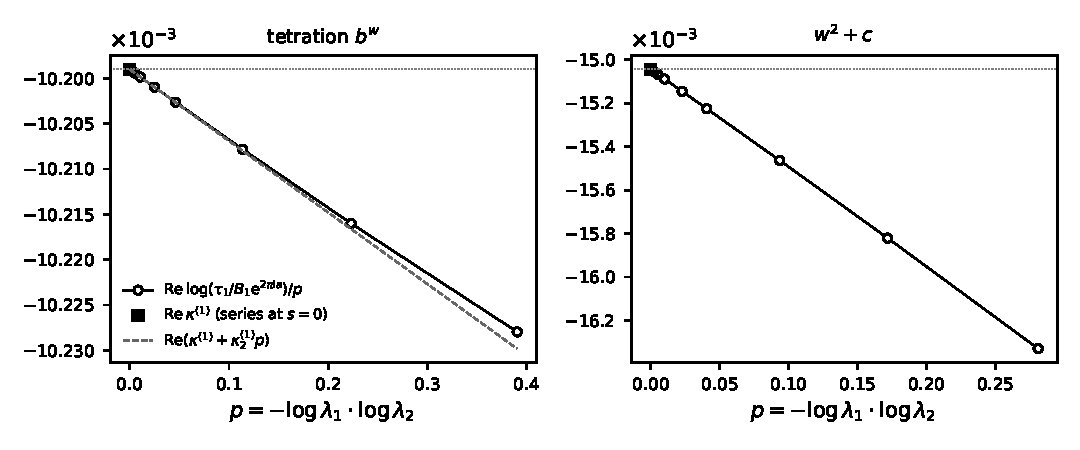
\includegraphics[width=\textwidth]{figures/fig8_deficit.pdf}
\caption{$\Rea\log(\tau_1/B_1\ee^{2\pi\ii a})/p$ 随 $p$ 的变化（圆圈，双曲侧直接计算，$\lambda_1=0.5,\dots,0.98$），
方块为 $s=0$ 处级数给出的 $\Rea\kappa^{(1)}$。左：tetration，虚线为 $\Rea(\kappa^{(1)}+\kappa^{(1)}_2p)$；右：二次族 $w^2+c$。数值。}
\label{ch8:fig:deficit}
\end{figure}

% ======================================================================
\notes

\paragraph{来源.}
本章是 \cite{KneserPaper} §5（The first-order term: a parabolic series）对一般实鞍结开折的改写。对应关系：
\cref{lem:uniform-model}–引理~5.1（对角元 $i/2$ 换成 $ia_2$，$D=8s$ 换成 $4\gamma s/a_2$）；\cref{ch8:lem:finite}–引理~5.2（$-2/u$ 换成 $-1/(a_2u)$）；
\cref{ch8:lem:derbounds}–引理~5.3；\cref{ch8:prop:diff}–命题~5.4；\cref{thm:first-order}–定理~5.6（$p'(0)=2$ 换成 $4a_2\gamma$）；
\cref{ch8:prop:higher}–命题~5.7；\cref{thm:all-orders}–定理~5.8（编号均指论文）。一般化的清单见论文定理~9.4 与 \texttt{docs/general-statements-zh.md} §2.6。
与论文相比，这里补了两处：\cref{lem:uniform-model}(3)（$e_i(0)=d_i$，论文只在注中说明）与除法公式 \eqref{ch8:eq:division}；
排斥侧的反射逆在一般情形下没有显式公式，只用到它对 $(s,v)$ 联合全纯。

\paragraph{思路.}
一致模型的想法来自 Mardešić--Roussarie--Rousseau 的预备形式 \cite{MRR2004}：在开折的整个参数邻域上同时正规化两个不动点。
发现``逐项求导发散''以及用一致模型修正的过程记录在 \texttt{docs/mrr-first-order-zh.md}。注意 \eqref{ch8:eq:Adot} 不同于朴素的 Hadamard 有限部分正则化：
后者的常数项一般不等于真导数，一致模型把正则化变成了精确恒等式。

\paragraph{变分公式.}
\cref{thm:first-order} 把 $\kappa^{(n)}$ 表示为一个收敛级数，但没有说明它的含义。第~\ref{ch:variation} 章证明
$\kappa^{(n)}=\kappa^{(n)}_{\mathrm{tr}}(g)+\Dfun_n(g)[X-X(0)]/(4a_2X(0))$：法向部分是芽的平移开折的一阶项，切向部分是 horn 不变量沿抛物层的导数。
那里的证明把本章的一致模型放进 Banach 空间 $\Ocal_r$ 中，作为 $f$ 的全纯函数。

% ======================================================================
\exercises

\begin{exercise}\label{ch8:ex:udot}
设 $u_k=g^k(u)$，$u\in P_R$。证明 $u_k=-\frac1{a_2k}+O(k^{-2}\log k)$，并由 $\dot u_{k+1}=g'(u_k)\dot u_k-X(u_k)$ 证明 $\dot u_k=-\frac{\gamma}3k+O(\log^2k)$。
\end{exercise}
\begin{hint}
令 $\dot u_k=k\,y_k$，得到 $y_{k+1}=y_k-\frac3k\bigl(y_k+\frac\gamma3\bigr)+O(k^{-2}\log k)$。
\end{hint}

\begin{exercise}\label{ch8:ex:divergence}
对第~\ref{ch:confluence} 章的（未修正的）模型时间，利用习题~\ref{ch8:ex:udot} 证明 $\partial_s[F_s(u_k)]_{s=0}+F_0'(u_k)\dot u_k\to-\frac{\gamma}{3a_2}\varphi_0(0)$，
其中 $F_0(u)=\varphi_0(0)u^2+O(u^3)$。对 tetration 求出 $\varphi_0(0)$，确认它不为零。
\end{exercise}

\begin{exercise}\label{ch8:ex:hadamard}
设 $G$ 在凸区域上全纯。证明 $(x,y)\mapsto(G(x)-G(y))/(x-y)$（对角线上取 $G'(x)$）联合全纯。由此补全 \cref{ch8:lem:removable} 中``被 $x-y$ 整除''一步。
\end{exercise}

\begin{exercise}\label{ch8:ex:p-holo}
用 \cref{ch8:lem:removable} 的论证（偶函数 $\Rightarrow$ $t^2$ 的函数）直接证明 $p=-\log\lambda_1\log\lambda_2$ 是 $s$ 的全纯函数，并对 tetration 验证 $p=2s+\frac{10}9s^2+O(s^3)$。
\end{exercise}

\begin{exercise}\label{ch8:ex:N2}
对 $g(u)=u+u^2$ 取 $N=3$。写出 \cref{lem:uniform-model} 证明中的 $4\times4$ 下三角矩阵 $M(0)$ 与 $\mathrm{rem}(\Phi_0)$，解出 $e(0)$，
并验证它给出形式 Abel 函数的系数 $d_1=-\frac12$、$d_2=\frac13$、$d_3=-\frac{13}{36}$、$d_4=\frac{113}{240}$（与 \cref{ch8:exa:quad-model} 的 $N=2$ 结果相容）。
\end{exercise}

\begin{exercise}\label{ch8:ex:exponent}
在 \cref{ch8:prop:diff} 的平衡中取 $J=s^{-\beta}$，求使误差最小的 $\beta$，证明误差为 $O(s^{2-8/(2N+3)})$。$N=2$ 时得到什么？
\end{exercise}

\begin{exercise}\label{ch8:ex:base}
由 \cref{prop:base-point} 证明：换基点使 $\kappa^{(n)}$ 改变 $\frac{2\pi\ii n}{4a_2\gamma}\Delta'(0)$，其中 $\Delta(s)=R_s^{-1}(w_0')$ 关于 $s$ 的导数在 $0^+$ 处存在。
所以 $\Rea\kappa^{(n)}$ 与基点无关。
\end{exercise}

\begin{exercise}\label{ch8:ex:CR}
设 $L_1=|\log\lambda_1|$、$L_2=\log\lambda_2$，$\epsilon_{\mathrm{CR}}=(A_2-A_1)^{-2}$，$\nu=A_1+A_2$。验证 $p=L_1L_2=4\epsilon_{\mathrm{CR}}/(1-\nu^2\epsilon_{\mathrm{CR}})$。
\end{exercise}

\begin{exercise}\label{ch8:ex:beyond}
设 $\phi(s)$ 在 $(0,s_0]$ 上有渐近展开 $\sum_ja_js^j$。证明 $\phi(s)+O(\Lam)$ 有同一个展开。由此说明 \cref{ch8:cor:sewing} 中 $\hat c_n$ 与 $\tau_n$ 的差别在任何阶的渐近展开中都看不见，
只能从指数小的尺度上看到。
\end{exercise}

\begin{exercise}\label{ch8:ex:fit}
用第~\ref{ch:confluence} 章数值一节的表中二次族的 $|\tau_1|/|B_1|-1$，通过对 $p$ 的二次拟合估计 $\Rea\kappa^{(1)}$，与级数值 $-0.0150441028391897$ 比较。
解释为什么 $(|\tau_1|/|B_1|-1)/p$ 与 $\Rea\log(\tau_1/B_1\ee^{2\pi\ii a})/p$ 只在 $O(p)$ 上不同。
\end{exercise}

\begin{exercise}\label{ch8:ex:second}
（较难）写出 $\kappa^{(n)}_2$ 用 $\cfA^{(1)},\cfA^{(2)},\cfS^{\sharp(1)},\cfS^{\sharp(2)}$ 及其导数在 $\ell$ 上的 Fourier 系数表示的公式。
\end{exercise}
\begin{hint}
先把 $v_s$ 展开到 $s^2$：$v_s=v+sV_1+s^2V_2+O(s^{2+\vartheta})$，$V_1=-\cfS^{\sharp(1)}/\Phirep'$，$V_2$ 由 $\cfS^\sharp_s(v_s)=z$ 的 $s^2$ 项确定；再展开 $\cfA_s(v_s)$，最后把 $s$ 换成 $p$。
\end{hint}

% 第 9 章 变分公式
% 来源：KneserPaper, sec-general.tex 小节 "The first-order term as a derivative on the
% parabolic stratum"（Lemma gen-banach, Prop. gen-linear, Thm gen-variation,
% Cor. gen-variation, Remarks gen-cocycle, gen-variation）；docs/kappa-variation-zh.md。
% 本章不新增宏。

\chapter{变分公式}\label{ch:variation}

第~\ref{ch:first-order} 章把一阶系数 $\kappa^{(n)}$ 写成了抛物轨道上的一个绝对收敛级数（\cref{thm:first-order}）。
级数给出了数值，却没有说明这个数「是什么」。本章回答这个问题。

答案是几何的。把所有靠近 $g$ 的映射放在一个 Banach 空间里。有二重不动点的映射构成一个复解析超曲面 $\Pstr$，
称为\textbf{抛物层}（parabolic stratum）。在实映射中，它把「有两个实不动点」的映射与「有一对复共轭不动点」的映射分开。
不变量 $\tau_n$ 定义在前一侧；在 $\Pstr$ 上，对应的量是 $B_n\ee^{2\pi\ii na}$。
我们证明：这两个量拼成的函数在 $g$ 处沿任何开折方向都有单侧导数，并且这个导数是一个连续线性泛函。
$\kappa^{(n)}$ 就是它沿开折方向 $X$ 的导数，按 $X=X(0)\cdot1+(X-X(0))$ 分成法向和切向两部分：
\[
 \kappa^{(n)}=\ktr^{(n)}(g)+\frac{\Dfun_n(g)\bigl[X-X(0)\bigr]}{4a_2X(0)} .
\]
切向部分是 horn 映射沿 $\Pstr$ 的导数，是抛物芽的形变理论里的对象；法向部分是芽 $g$ 的一个数 $\ktr^{(n)}(g)$。

这个分解立刻回答了「$\kappa^{(n)}$ 有没有闭式」的问题：同一个芽配不同的开折方向，$\operatorname{Re}\kappa^{(n)}$ 可以从 $-0.0102$ 变到 $395$，
所以 $\kappa^{(n)}$ 不是芽的函数。它还说明 tetration 为什么是「标准」例子：底数方向与平移方向只差一个无穷小共轭。

\begin{goals}
\item 同调算子 $\Lop\phi=\phi\circ g-g'\phi$ 描述无穷小共轭；它的形式余核是 $\operatorname{span}\{1,u^3\}$。
\item 抛物层 $\Pstr$ 是复解析超曲面，$T_g\Pstr=\{Y:Y(0)=0\}$；常数方向 $1$ 是法向。
\item 一致模型对 Banach 参数全纯，由此得到连续线性泛函 $\Lfun_n$，它同时给出开折的一阶项和 $\Pstr$ 上的导数。
\item 变分公式（\cref{thm:variation}）：$\kappa^{(n)}$ = 法向常数 $\ktr^{(n)}(g)$ + horn 不变量的切向导数。
\item $\operatorname{Re}\kappa^{(n)}$ 只依赖开折方向模 $\Lop$ 的类；$\ktr^{(n)}$ 在坐标变换下按上闭链变化，不是芽的不变量。
\item horn 变分由正则化的轨道级数（Melnikov 型公式）计算；数值上公式两边吻合到 $10^{-17}$（$n=1$）。
\end{goals}

%====================================================================
\section{问题：一阶系数依赖什么}\label{ch9:sec:question}

回忆第~\ref{ch:unfolding} 章的设定（\cref{def:unfolding}）。$g(u)=u+a_2u^2+a_3u^3+\cdots$ 是实抛物芽，$a_2>0$；
开折 $f_s$ 满足
\begin{equation}\label{ch9:eq:direction}
 f_s=g-sX+O(s^2),\qquad \gamma=X(0)>0 .
\end{equation}
我们称 $X$ 为开折的\textbf{方向}（direction）。由 \cref{prop:scales}，$p=-\log\lambda_1\log\lambda_2=4a_2\gamma s+O(s^2)$。
第~\ref{ch:first-order} 章证明了：若 $B_n\ne0$，则
\begin{equation}\label{ch9:eq:kappa-recall}
 \log\frac{\tau_n}{B_n\ee^{2\pi\ii na}}=\kappa^{(n)}p+O(p^{10/9}),\qquad
 \kappa^{(n)}=\frac{\delta t_n}{4a_2\gamma B_n}-\frac{2\pi\ii n\,\delta t_0}{4a_2\gamma},
\end{equation}
其中 $\delta t_m$ 是闸门线上函数 $\delta T$ 的 Fourier 系数，$\delta T$ 由正则化的轨道级数给出（\cref{thm:first-order}；全阶版本见 \cref{thm:all-orders}）。

\begin{lemma}\label{ch9:lem:first-jet}
$\kappa^{(n)}$ 只依赖于芽 $g$、方向 $X$ 和基点 $\ustar$，与 $f_s$ 的 $O(s^2)$ 项无关。
\end{lemma}

\begin{proof}
在 \cref{thm:first-order} 的公式里，参数只通过三处进入：一致模型时间 $\Psi_s$ 对 $s$ 的导数、一步误差 $F_s$ 对 $s$ 的导数、
以及轨道导数 $\dot u_k=\partial_sf_s^k(u)|_{s=0}$。由链式法则，前两者只依赖 $\partial_sf_s|_{s=0}=-X$，
而 $\dot u_k$ 满足递推 $\dot u_{k+1}=g'(u_k)\dot u_k-X(u_k)$，$\dot u_0=0$，也只依赖 $X$。
最后 $p'(0)=4a_2\gamma$ 只依赖 $X(0)$。
\end{proof}

所以我们可以写 $\kappa^{(n)}=\kappa^{(n)}[g;X]$。它是 $X$ 的什么样的函数？\cref{ch9:tab:preview} 给出了第一个线索。

\begin{table}[htbp]
\centering\small
\caption{同一个芽 $g=\ee^u-1$、不同方向 $X$ 的一阶系数（$n=1$，基点 $\ustar=1/\ee-1$）。
数据来自 \texttt{docs/kappa\_variation.py}，45 位运算，输出文件 \texttt{docs/data/kappa-variation-exp.txt}。}
\label{ch9:tab:preview}
\begin{tabular}{lll}
\toprule
方向 $X$ & $\operatorname{Re}\kappa^{(1)}$ & $\operatorname{Im}\kappa^{(1)}$\\
\midrule
$1$ & $-0.0101990063458974$ & $19.1021373259046$\\
$(1+u)\ee^u$（tetration） & $-0.0101990063458974$ & $-0.0132509561825067$\\
$1+0.6u^2$ & $39.5149228923293$ & $62.4195598999261$\\
$1+0.3u+0.5u^4$ & $395.094296950776$ & $-224.037840614510$\\
\bottomrule
\end{tabular}
\end{table}

表中有两个现象。第一，$\operatorname{Re}\kappa^{(1)}$ 随方向剧烈变化，因此 $\kappa^{(n)}$ 不可能只是 $g$（或 $B_n$、$a$、$\rho$）的函数。
第二，平移方向 $X=1$ 与 tetration 的方向 $X=(1+u)\ee^u$ 给出相同的实部，虚部却不同。
本章的目标是解释这两个现象：实部只依赖于 $X$ 模无穷小共轭的类（\cref{ch9:sec:homological}），
而对这个类的依赖是仿射的，斜率是 horn 不变量沿抛物层的导数（\cref{ch9:sec:formula}）。

%====================================================================
\section{同调算子与无穷小共轭}\label{ch9:sec:homological}

\subsection{定义}
固定 $r>0$ 足够小，使 $g$ 在 $D_{2r}=\{|u|<2r\}$ 上全纯且 $g(\overline{D_r})\subset D_{2r}$。
记 $\Ocal_r$ 为 $D_r$ 上有界全纯函数构成的 Banach 空间，范数为上确界范数。

\begin{definition}\label{ch9:def:Lop}
芽 $g$ 的\textbf{同调算子}（homological operator）是
\[
 \Lop:\Ocal_{2r}\to\Ocal_r,\qquad \Lop\phi=\phi\circ g-g'\,\phi .
\]
它是有界线性算子。若 $\phi$ 在实轴上取实值，就称 $\phi$ 是实的。
\end{definition}

这个算子的意义是下面的计算。

\begin{lemma}[无穷小共轭]\label{ch9:lem:infinitesimal-conjugacy}
设 $\phi\in\Ocal_{2r}$，$\psi_t=\id+t\phi$。则对 $|t|$ 足够小，在 $D_{r/2}$ 上
\[
 \psi_t^{-1}\circ g\circ\psi_t=g-t\,\Lop\phi+O(t^2) .
\]
更一般地，若 $f_s=g-sX+O(s^2)$，则 $\psi_s^{-1}\circ f_s\circ\psi_s=g-s(X+\Lop\phi)+O(s^2)$。
这里的 $O(\cdot)$ 是在 $\Ocal_{r/2}$ 的范数下。
\end{lemma}

\begin{proof}
$g\circ\psi_t(u)=g(u+t\phi(u))=g(u)+t\,g'(u)\phi(u)+O(t^2)$。
又 $\psi_t^{-1}(v)=v-t\phi(v)+O(t^2)$（由 $\psi_t(\psi_t^{-1}v)=v$ 比较一阶项）。代入 $v=g\circ\psi_t(u)=g(u)+O(t)$ 得
\[
 \psi_t^{-1}\circ g\circ\psi_t=g+t\,g'\phi-t\,\phi\circ g+O(t^2)=g-t\Lop\phi+O(t^2).
\]
所有余项都由 Cauchy 估计在 $D_{r/2}$ 上一致控制。第二个公式同理：$f_s$ 的 $-sX$ 项在共轭下只产生 $-sX+O(s^2)$。
\end{proof}

于是，把方向 $X$ 换成 $X+\Lop\phi$（$\phi$ 实）相当于在一阶上对开折作实解析共轭 $\psi_s=\id+s\phi$。结合 \cref{ch9:lem:first-jet} 与 \cref{cor:invariance}，这已经提示 $\operatorname{Re}\kappa^{(n)}$ 在这个替换下不变；\cref{cor:variation} 将在本章的局部设定下直接证明这一点。
注意 $\Lop\phi(0)=\phi(0)-g'(0)\phi(0)=0$，所以这个替换不改变横截性 $\gamma=X(0)$。

\subsection{形式余核}
在形式幂级数环 $\C[[u]]$ 上同样定义 $\Lop\phi=\phi\circ g-g'\phi$。

\begin{proposition}\label{ch9:prop:formal-coker}
\begin{enumerate}
\item 对每个 $k\ge0$，
\[
 \Lop(u^k)=(k-2)a_2\,u^{k+1}+\Bigl((k-3)a_3+\tbinom k2a_2^2\Bigr)u^{k+2}+O(u^{k+3}) .
\]
\item $\C[[u]]=\C\cdot1\ \oplus\ \C\cdot u^3\ \oplus\ \Lop(\C[[u]])$（直和）。
\item $\ker\Lop$ 是一维的，由一个首项为 $u^2$ 的级数张成。
\end{enumerate}
\end{proposition}

\begin{proof}
(1) 由二项式展开，
$g(u)^k=u^k(1+a_2u+a_3u^2+\cdots)^k=u^k+ka_2u^{k+1}+\bigl(ka_3+\binom k2a_2^2\bigr)u^{k+2}+\cdots$，
而 $g'(u)u^k=u^k+2a_2u^{k+1}+3a_3u^{k+2}+\cdots$。相减即得。

(2) 记 $[Y]_j$ 为 $Y$ 中 $u^j$ 的系数。由 (1)，$\Lop(u^k)$ 从 $u^{k+1}$ 开始，首项系数 $(k-2)a_2$ 仅在 $k=2$ 时为零。

\emph{生成.} 给定 $Y\in\C[[u]]$，我们逐阶构造 $\phi=\sum\phi_ku^k$。因为 $\Lop\phi$ 没有常数项，必须取 $c_0=[Y]_0$。
比较 $u^1,u^2$ 的系数，依次解出 $\phi_0=-[Y]_1/(2a_2)$ 与 $\phi_1$（首项系数 $-a_2\ne0$）。
$u^3$ 的系数中 $\phi_2$ 的贡献为零（因 $(2-2)a_2=0$），而 $\phi_k$（$k\ge3$）不贡献，
所以令 $c_3=[Y]_3-[\Lop(\phi_0+\phi_1u)]_3$，并取 $\phi_2=0$。
对 $j\ge4$，$u^j$ 的系数方程是 $(j-3)a_2\phi_{j-1}+(\text{已定的量})=[Y]_j$，可唯一解出 $\phi_{j-1}$。
于是 $Y=c_0+c_3u^3+\Lop\phi$。

\emph{直和.} 设 $c_0+c_3u^3=\Lop\phi$。常数项给出 $c_0=0$；$u^1,u^2$ 的系数依次给出 $\phi_0=\phi_1=0$；
这时 $[\Lop\phi]_3=0$，故 $c_3=0$。

(3) 若 $\Lop\phi=0$，上一段的论证给出 $\phi_0=\phi_1=0$，而 $\phi_2$ 任意；$\phi_2$ 确定之后，$u^j$（$j\ge4$）的方程唯一确定 $\phi_{j-1}$。
所以 $\ker\Lop$ 由 $\phi_2=1$ 的唯一解张成。
\end{proof}

\begin{remark}[余核的解释]\label{ch9:rem:coker-meaning}
两个余核方向各有含义。方向 $1$ 是开折参数本身：$g-s$ 把二重不动点分裂开。
方向 $u^3$ 对应迭代留数 $\rho=1-a_3/a_2^2$ 的变化：对 $Y=y_2u^2+y_3u^3+\cdots$，沿 $g-tY$ 有
\[
 \frac{\dd\rho}{\dd t}\Big|_{t=0}=\frac{a_2y_3-2a_3y_2}{a_2^3},
\]
而 $\rho$ 是芽在保持 $0$ 的（形式）共轭下的不变量（线性换元同时缩放 $a_2$ 与 $a_3$，比值 $a_3/a_2^2$ 不变），所以它在 $\Lop\phi$（$\phi=O(u)$，此时 $\Lop\phi=O(u^2)$）上的导数为零（\cref{ch9:ex:drho}）。
这与开折的形式分类相符：鞍结开折的形式不变量是一个参数和一个留数函数\cite{ChristopherRousseau}。
$\ker\Lop$ 的生成元是 $g$ 的形式无穷小生成元（\cref{ch9:ex:kernel}）。

在解析范畴里，$\Ocal_r/\Lop(\Ocal_{2r})$ 远比 $\operatorname{span}\{1,u^3\}$ 大：芽的解析分类除形式不变量外还有 \'Ecalle--Voronin 模，
它是无穷维的\cite{Ecalle1981,Voronin1981}。启发式地说，多出来的余核方向就是模空间的切方向。
本章不需要、也不证明这一说法；下面用到的只是 $\Lop$ 的像在一个具体意义下「对实部不可见」（\cref{cor:variation}）。
\end{remark}

\begin{example}\label{ch9:ex:coboundaries}
三个具体的上边界（即 $\Lop$ 的像中的元素）。
\begin{enumerate}
\item 二次芽 $g=u+u^2$：$\Lop(u)=u+u^2-(1+2u)u=-u^2$。
\item 指数芽 $g=\ee^u-1$：$\Lop(u)=\ee^u-1-u\ee^u$。
\item 指数芽与常数加线性函数：$\Lop(-2-u)=(-2-(\ee^u-1))-\ee^u(-2-u)=(1+u)\ee^u-1$。
\end{enumerate}
第三个等式说：tetration 的方向 $X=(1+u)\ee^u$（\cref{ch9:ex:tetration-direction}）满足 $X-1\in\Lop(\Ocal_{2r})$。
\end{example}

\begin{example}\label{ch9:ex:tetration-direction}
tetration 的族 $w\mapsto b^w$ 在仿射坐标 $w=\ee(1+u)$ 下是 $f_s(u)=\ee^{-s+(1-s)u}-1$，$s=1-\ee\log b$，基点 $w_0=1$ 对应 $\ustar=1/\ee-1$。对 $s$ 求导，
$\partial_sf_s(u)|_{s=0}=-(1+u)\ee^u$，所以 $X=(1+u)\ee^u$，$\gamma=1$，$a_2=\tfrac12$，$4a_2\gamma=2=p'(0)$。
对二次族 $w^2+c$，取 $w=\tfrac12+u$、$c=\tfrac14-s$，得 $f_s(u)=u+u^2-s$，这是平移开折，$X=1$。
对 $v-\sin v+c$，取 $v=\tfrac\pi2+u$、$c=1-s$，得 $f_s(u)=u+(1-\cos u)-s$，也是平移开折。
\end{example}

%====================================================================
\section{抛物层}\label{ch9:sec:stratum}

\subsection{对称函数与判别式}
设 $f\in\Ocal_r$ 靠近 $g$。因为 $g(u)-u=a_2u^2(1+O(u))$ 在圆周 $|u|=r/2$ 上不为零（$r$ 小），由 Rouché 定理，
当 $\|f-g\|$ 足够小时，$f-\id$ 在 $D_{r/2}$ 内恰有两个零点（计重数），记为 $u_1[f],u_2[f]$。

\begin{lemma}\label{ch9:lem:symmetric}
存在 $g$ 在 $\Ocal_r$ 中的邻域 $U$，使下面的量都是 $f\in U$ 的全纯函数：
\[
 e_1[f]=u_1+u_2,\qquad e_2[f]=u_1u_2,\qquad D[f]=e_1^2-4e_2=(u_1-u_2)^2,
\]
以及 Weierstrass 分解 $f(u)-u=q[f](u)\,\mathsf k[f](u)$ 中的二次多项式 $q[f](u)=u^2-e_1u+e_2$ 和余因子 $\mathsf k[f]\in\Ocal_{r/2}$，
$\mathsf k[f]$ 在 $D_{r/2}$ 上无零点，$\mathsf k[g](0)=a_2$。并且 $e_2[f]=f(0)/\mathsf k[f](0)$。
\end{lemma}

\begin{proof}
由辐角原理，对 $j=1,2$，
\[
 u_1^j+u_2^j=\frac1{2\pi\ii}\oint_{|u|=r/2}u^j\,\frac{f'(u)-1}{f(u)-u}\,\dd u .
\]
被积函数在圆周上关于 $f$ 全纯（$f\mapsto f'(u)$ 是有界线性映射，$f(u)-u$ 在圆周上远离零），所以幂和关于 $f$ 全纯，
$e_1=u_1+u_2$，$e_2=\tfrac12\bigl(e_1^2-(u_1^2+u_2^2)\bigr)$ 也是。
余因子 $\mathsf k[f]=(f-\id)/q[f]$ 在 $D_{r/2}$ 内全纯（零点相消），并由 Cauchy 积分
$\mathsf k[f](u)=\frac1{2\pi\ii}\oint_{|\zeta|=r/2}\frac{f(\zeta)-\zeta}{q[f](\zeta)(\zeta-u)}\,\dd\zeta$（$|u|<r/2$）关于 $f$ 全纯。
在 $u=0$ 处 $f(0)=q[f](0)\mathsf k[f](0)=e_2\mathsf k[f](0)$。$\mathsf k[g](u)=(g(u)-u)/u^2$，故 $\mathsf k[g](0)=a_2$。
这是 Weierstrass 预备定理（\cref{thm:weierstrass-prep}）带 Banach 参数的形式，这里的积分公式直接给出了参数全纯性。
\end{proof}

这里「全纯」是 Banach 空间意义下的：映射在每点 Fr\'echet 复可微。本章反复使用下面的经典事实\cite[§§5--8]{Mujica1986}：
一个局部有界的映射，若在每条复直线上全纯（G-全纯），则全纯；全纯映射的复合、Cauchy 积分、一致收敛极限仍然全纯；
全纯映射有 Cauchy 估计。另见附录~\ref{app:tools}。

\subsection{抛物层是超曲面}

\begin{definition}\label{ch9:def:stratum}
$g$ 附近的\textbf{抛物层} $\Pstr$ 是 $U$ 中在 $D_{r/2}$ 内有二重不动点的映射的集合，即 $\Pstr=\{f\in U:D[f]=0\}$。
$Y\in\Ocal_r$ 称为 $\Pstr$ 在 $g$ 处的\textbf{切向量}，指存在 $\Pstr$ 中的曲线 $g-tY+O(t^2)$。
\end{definition}

注意切向量的符号约定：切向量 $Y$ 对应的曲线是 $g-tY$，与开折 $f_s=g-sX$ 的约定一致。

\begin{proposition}\label{ch9:prop:submersion}
\begin{enumerate}
\item $D$ 在 $g$ 处是淹没：$\dd D[g](H)=-4H(0)/a_2$，其中 $\dd D[g](H)$ 表示沿曲线 $g+tH$ 的导数。
\item $\Pstr$ 在 $g$ 附近是 $\Ocal_r$ 中的复解析超曲面，切空间为
\[
 T_g\Pstr=\{Y\in\Ocal_r:\ Y(0)=0\} .
\]
\item 每个 $Y\in T_g\Pstr$ 都是 $\Pstr$ 中一条全纯曲线 $t\mapsto g-tY+c(t)\cdot1$ 的切向量，其中 $c$ 全纯，$c(t)=O(t^2)$。
若 $Y$ 是实的，这条曲线由实映射组成。
\end{enumerate}
\end{proposition}

\begin{proof}
(1) 因 $e_1[g]=0$，$\dd(e_1^2)[g]=2e_1[g]\,\dd e_1[g]=0$。由 \cref{ch9:lem:symmetric}，
$e_2[g+tH]=(g+tH)(0)/\mathsf k[g+tH](0)=tH(0)/\mathsf k[g+tH](0)$，所以 $\dd e_2[g](H)=H(0)/a_2$。于是 $\dd D[g](H)=-4H(0)/a_2$。
这个线性泛函不为零（取 $H=1$）。

(2) $\ker\dd D[g]=\{H:H(0)=0\}$ 有闭补空间 $\C\cdot1$。由 Banach 空间上的隐函数定理，
存在 $\ker\dd D[g]$ 中 $0$ 的邻域上的全纯函数 $c$，$c(0)=0$，$\dd c(0)=0$，使在 $g$ 附近
$D[g+H+c\cdot1]=0$（$H\in\ker\dd D[g]$）当且仅当 $c=c(H)$。所以 $\Pstr$ 局部是图像 $\{g+H+c(H)\cdot1\}$，切空间是 $\ker\dd D[g]$。

(3) 取 $H=-tY$，曲线 $t\mapsto g-tY+c(-tY)\cdot1$ 在 $\Pstr$ 中。因 $\dd c(0)=0$，$c(-tY)=O(t^2)$。
若 $Y$ 实，记 $f^\star(u)=\overline{f(\bar u)}$。$D[f^\star]=\overline{D[f]}$，所以 $c(H^\star)=\overline{c(H)}$，由唯一性，实 $H$ 给出实 $c(H)$。
\end{proof}

\begin{remark}[实的图景]\label{ch9:rem:real-picture}
对实的 $f\in U$，$D[f]$ 是实数。$D>0$ 时两个不动点 $u_1<u_2$ 是实的；由 $f(u)-u=q\mathsf k$ 和 $\mathsf k>0$，
$f'(u_1)=1+(u_1-u_2)\mathsf k(u_1)<1<f'(u_2)$，所以左边的不动点自动是吸引的。$D<0$ 时两个不动点复共轭。
对开折 \eqref{ch9:eq:direction}，$D[f_s]=4\gamma s/a_2+O(s^2)$，这正是 \cref{prop:scales} 证明中出现的判别式。
所以 $\gamma>0$ 等价于：开折曲线在 $g$ 处横截 $\Pstr$，并进入 $D>0$ 的一侧。
\end{remark}

\begin{figure}[htbp]
\centering
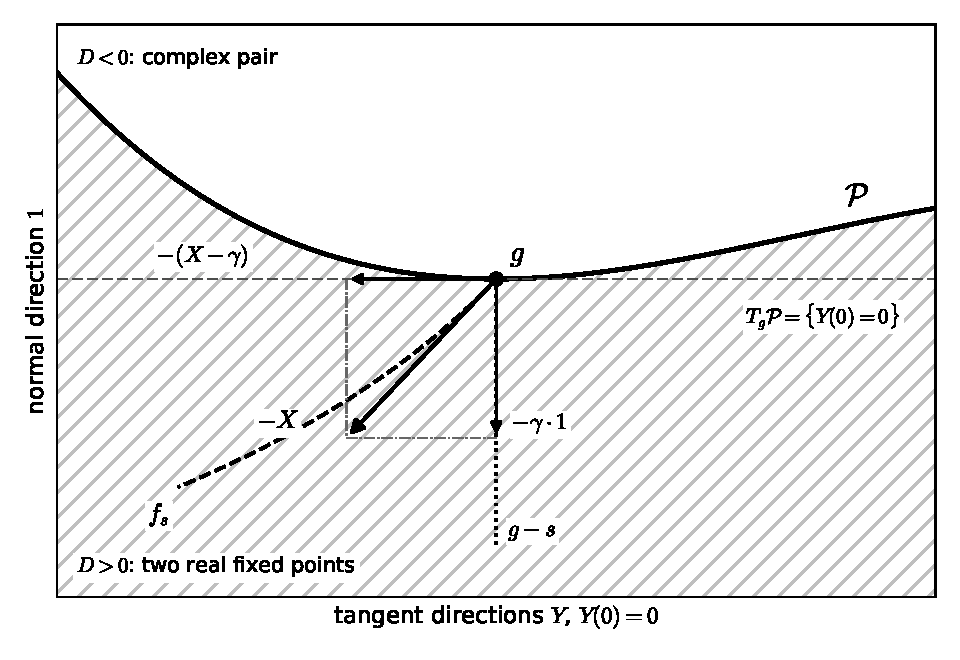
\includegraphics[width=0.78\textwidth]{figures/fig9_stratum.pdf}
\caption{$g$ 附近映射空间的示意图。横轴代表切方向 $T_g\Pstr=\{Y(0)=0\}$，纵轴代表常数方向 $1$。
粗实线是抛物层 $\Pstr$；阴影区 $D>0$ 是有两个实不动点的实映射，上方 $D<0$ 是有一对复共轭不动点的映射。
虚线是开折 $f_s=g-sX+O(s^2)$，其速度 $-X$ 分解为法向分量 $-\gamma\cdot1$ 与切向分量 $-(X-\gamma)$。
点线是平移开折 $g-s$。（脚本 \texttt{figures/fig9\_stratum.py}）}
\label{ch9:fig:stratum}
\end{figure}

\cref{ch9:fig:stratum} 是本章的几何图景。不变量 $\tau_n$ 定义在阴影区；我们要说明它与 $\Pstr$ 上的 $B_n\ee^{2\pi\ii na}$
拼成一个在 $g$ 处「一阶光滑」的函数，然后对这个函数的导数作切向、法向分解。

%====================================================================
\section{一致模型的 Banach 全纯性}\label{ch9:sec:banach}

本节把第~\ref{ch:first-order} 章的一致模型（\cref{lem:uniform-model}）从单参数族推广到 Banach 参数。
回忆它的构造。对 $f$ 靠近 $g$，令 $u_1,u_2$ 为 $f$ 在 $D_{r/2}$ 内的不动点，$q=q[f]$，$\mathsf k=\mathsf k[f]$，
\[
 A[f](x,y)=\frac1{\log\bigl(1+(x-y)\mathsf k[f](x)\bigr)},\qquad A_1=A[f](u_1,u_2),\quad A_2=A[f](u_2,u_1),
\]
所以 $D[f]\ne0$ 时 $A_j=1/\log f'(u_j)$。取整数 $N\ge1$，一致模型时间与一步误差为
\begin{align*}
 \Psi[f](u)&=A_1\log(u-u_1)+A_2\log(u-u_2)+P[f](u),\\
 F[f](u)&=\Psi[f](f(u))-\Psi[f](u)-1,
\end{align*}
其中 $P[f]=\sum_{i=1}^{2N-2}\mathsf p_i[f]u^i$ 是使 $F[f]$ 被 $q[f]^N$ 整除的多项式；对数分支按 \cref{lem:uniform-model}(1) 的约定，
即 $|u|>\delta$ 时 $\log(u-u_j)=\log u+\Log(1-u_j/u)$。记 $\nu[f]=A_1+A_2$。

\begin{lemma}\label{ch9:lem:banach}
固定 $N\ge3$。缩小 $r$ 之后，在 $g$ 于 $\Ocal_r$ 中的某个邻域上：
\begin{enumerate}
\item $\nu[f]$ 和一步误差 $F[f]=q[f]^N\Gamma[f]$ 关于 $f$ 全纯，后者取值于 $D_{r/2}$ 上有界全纯函数的空间；
\item 对每个 $\delta\in(0,r/2)$，在一个（更小的）邻域上，模型时间 $\Psi[f]-\nu[f]\log u$ 关于 $f$ 全纯，取值于圆环 $\delta<|u|<r/2$ 上有界全纯函数的空间；
\item 对反射逆映射 $G[f](v)=-f^{-1}(-v)$ 同样成立。
\end{enumerate}
\end{lemma}

\begin{proof}
\cref{lem:uniform-model} 的证明由三步组成，我们逐步检查它们对 Banach 参数的全纯依赖。

\emph{第一步：预备与除法。} $e_1,e_2,q[f],\mathsf k[f]$ 关于 $f$ 全纯（\cref{ch9:lem:symmetric}）。
Weierstrass 除法 $\chi=q[f]\cdot(\text{商})+(\text{余式})$ 由 Cauchy 积分给出，商和余式都关于 $(f,\chi)$ 全纯。

\emph{第二步：对角线上的可去性。} 令 $\chi(x)$ 是 $(f,x,y,u)$ 的全纯函数。考虑
\[
 \Theta=A[f](x,y)\,\chi(y)+A[f](y,x)\,\chi(x),\qquad \Theta'=A[f](x,y)\,\chi(x)+A[f](y,x)\,\chi(y).
\]
由 $1/\log(1+z)=1/z+\tfrac12+O(z)$，$A[f](x,y)=\frac1{(x-y)\mathsf k[f](x)}+\tfrac12+(x-y)\mathsf q[f](x,y)$，$\mathsf q$ 全纯。
所以 $\Theta$ 的奇异部分是 $\bigl[\chi(y)/\mathsf k(x)-\chi(x)/\mathsf k(y)\bigr]/(x-y)$，分子在对角线 $x=y$ 上为零；
$\Theta'$ 的奇异部分 $\bigl[\chi(x)/\mathsf k(x)-\chi(y)/\mathsf k(y)\bigr]/(x-y)$ 同样可去。
因此 $\Theta,\Theta'$ 是 $(f,x,y,u)$ 的全纯函数，且关于 $x,y$ 对称。对称的全纯函数是初等对称函数 $(x+y,xy)$ 的全纯函数
（对每个固定的其他变量，这是关于两个变量的对称收敛幂级数的经典事实；参数依赖由 Cauchy 积分表示保持）。
代入 $(x+y,xy)=(e_1[f],e_2[f])$，得到 $f$ 的全纯函数。应用于
\begin{itemize}
\item $\chi\equiv1$ 于 $\Theta'$：得到 $\nu[f]$；
\item $\chi(x)=\Log(1-x/u)$ 于 $\Theta'$（$|u|>\delta$，$|u_j|<\delta/2$）：得到 $\Psi[f]-\nu[f]\log u-P[f]$；
\item $\chi(x)=\log\bigl(1+(u-x)\mathsf k[f](u)\bigr)$ 于 $\Theta$：得到 $F^{\log}[f]=A_1\log\frac{f-u_1}{u-u_1}+A_2\log\frac{f-u_2}{u-u_2}-1$，
  因为 $(f(u)-u_1)/(u-u_1)=1+(u-u_2)\mathsf k(u)$。
\end{itemize}

\emph{第三步：线性方程组.} $D[f]\ne0$ 时 $F^{\log}[f](u_j)=A_j\log f'(u_j)-1=0$，所以 $F^{\log}[f]$ 被 $q[f]$ 除的余式在两个不同点为零，
是零。余式关于 $f$ 全纯，而 $\{D\ne0\}$ 在 $U$ 中稠密，所以余式恒为零：$F^{\log}[f]=q[f]\varphi[f]$，$\varphi$ 全纯。
同理 $u\mapsto f(u)^i-u^i=q[f]\,d_i[f]$。把 $\varphi+\sum_i\mathsf p_id_i$ 除以 $q[f]^{N-1}$，余式的 $2N-2$ 个系数关于 $f$ 全纯、关于 $\mathsf p=(\mathsf p_i)$ 仿射，
矩阵记为 $M[f]$。在 $f=g$ 处余式就是模 $u^{2N-2}$ 的 Taylor 多项式，$d_i[g]=ia_2u^{i-1}+O(u^i)$，所以 $M[g]$ 是下三角的，
对角元 $ia_2\ne0$。于是在 $g$ 附近 $\mathsf p[f]=-M[f]^{-1}\operatorname{rem}(\varphi[f])$ 关于 $f$ 全纯，且 $F[f]=q[f]^N\Gamma[f]$，$\Gamma[f]$ 全纯。

每一步都把全纯映射复合、作 Cauchy 积分或求逆，所以结论成立。对 $G[f]$，先用 Banach 空间上的反函数定理得到 $f\mapsto f^{-1}$ 在 $D_{r/2}$ 附近全纯，
再重复上面的论证。
\end{proof}

\begin{remark}
\cref{ch9:lem:banach} 是本章唯一的技术性输入。它说的是：第~\ref{ch:first-order} 章里所有对 $s$ 的全纯依赖，
其实是对整个映射 $f$ 的全纯依赖，$s$ 只是通过 $f_s$ 进入。由此，任何「对 $s$ 求导」都可以改写成「沿方向 $-X$ 的方向导数」。
\end{remark}

%====================================================================
\section{线性泛函 \texorpdfstring{$\Lfun_n$}{L\_n}}\label{ch9:sec:linear}

\subsection{设定}
本章所说的\textbf{开折}，指实解析曲线 $s\mapsto f_s\in\Ocal_r$，$f_0=g$，满足 \eqref{ch9:eq:direction} 与 $\gamma>0$。
不需要 \cref{def:unfolding} 中 (H1) 那样的整体假设：我们用的 $\tau_n$ 是闸门线上局部转移 $\mathcal A\circ(\mathcal S^\sharp)^{-1}$ 的不变量
$t_n\ee^{-2\pi\ii nt_0}$，而这正是 \cref{thm:reduction}、\cref{thm:confluence} 与第~\ref{ch:first-order} 章的证明所使用的全部内容。
基点取为实数 $\ustar\in(-r/2,0)$，满足 $g$ 在 $[\ustar,0]$ 上递增且 $g(u)>u$（$u\in[\ustar,0)$）；
对 $f$ 靠近 $g$，同样的性质在吸引不动点左侧成立。对整函数族（满足 (H1)），基点可以像第~\ref{ch:first-order} 章那样用 $f^m$ 搬运到远处，论证不变。

记 $\ell=[0,1]+\ii Y_*$ 为闸门线（\cref{thm:confluence}），$v(z)=\Phirep[g]^{-1}(z)$。对 $f$ 靠近 $g$，令
\[
 \mathcal A[f](u)=\Psi[f](u)+\sum_{k\ge0}F[f](f^ku)
\]
（在吸引花瓣中；在其余的基本域上用 $\mathcal A[f]\circ f^m-m$ 延拓），$\mathcal S[f]$ 为反射族 $G[f]$ 的同样构造给出的排斥时间。

\begin{definition}\label{ch9:def:invariant}
对实的 $f$ 靠近 $g$、有两个实不动点（$D[f]>0$），令 $\Ifun_n[f]=\tau_n[f]$；对 $f\in\Pstr$，令
\[
 \Ifun_n[f]=B_n[f]\,\ee^{2\pi\ii na[f]},
\]
其中 $B_n[f]$、$a[f]=\Phiatt[f](\ustar)$ 由 $f$ 在其二重不动点处的芽计算（\cref{def:horn}，用该芽的形式 Abel 函数归一化），基点仍是 $\ustar$。
\end{definition}

两种情形下，$\Ifun_n[f]$ 都是闸门线上转移 $T=\mathcal A[f]\circ\mathcal S^\sharp[f]^{-1}$ 的不变量 $t_n\ee^{-2\pi\ii nt_0}$，
其中 $\mathcal A[f]$ 按 $\mathcal A[f](\ustar)=0$ 归一化（\cref{thm:reduction} 与第~\ref{ch:first-order} 章）。

\begin{remark}[归一化的重要性]\label{ch9:rem:normalization}
这个归一化不是装饰。吸引一侧加一个常数 $c$，$T$ 变成 $T+c$，$t_0\mapsto t_0+c$，于是 $t_n\ee^{-2\pi\ii nt_0}$ 乘上 $\ee^{-2\pi\ii nc}$；
排斥一侧加常数 $c$，$T(z)$ 变成 $T(z-c)$，$t_n\mapsto t_n\ee^{-2\pi\ii nc}$，$t_0\mapsto t_0-c$，$t_n\ee^{-2\pi\ii nt_0}$ 不变。
所以只有吸引一侧需要钉住，钉在基点上。这也是 $a$ 出现在极限 $B_n\ee^{2\pi\ii na}$ 中的原因（参见 \cref{prop:base-point}）。
\end{remark}

由 \cref{thm:confluence}，$\Ifun_n$ 在 $g$ 处从 $D>0$ 的一侧连续：$\Ifun_n[f_s]\to\Ifun_n[g]$。

\subsection{泛函的定义}
在第~\ref{ch:first-order} 章 \cref{thm:first-order} 的 $\dot\tau_n$ 公式里，把每个对 $s$ 的导数换成沿 $-X$ 的方向导数：
对 $u$ 在花瓣的紧子集 $K$ 中，令
\begin{equation}\label{ch9:eq:Adot}
 \dot{\mathcal A}[X](u)=\dd\Psi[g](-X)(u)+\sum_{k\ge0}\Bigl[\dd F[g](-X)(u_k)+F[g]'(u_k)\,\dot u_k\Bigr],
\end{equation}
其中 $u_k=g^k(u)$，$\dot u_{k+1}=g'(u_k)\dot u_k-X(u_k)$，$\dot u_0=0$。在基点和花瓣以外的基本域上，用 $\dot{\mathcal A}=\dot{\mathcal A}\circ g^m+\mathcal A[g]'\circ g^m\cdot\dot u_m$ 延拓。
排斥一侧由 $G$ 同样定义 $\dot{\mathcal S}^\sharp[X]$，其中 $\mathcal S^\sharp$ 在闸门中一个固定参考点 $u_\sharp$ 处的值 $\Phirep[g](u_\sharp)$ 保持不变（第~\ref{ch:first-order} 章的归一化）。令
\begin{gather*}
 \delta T[X](z)=\dot{\mathcal A}[X](v(z))-\dot{\mathcal A}[X](\ustar)-\tilde T_0'(z)\,\dot{\mathcal S}^\sharp[X](v(z)),\\
 \tilde T_0=\horn^{-1}-a,\qquad
 \delta t_m[X]=\int_\ell\delta T[X](z)\,\ee^{-2\pi\ii mz}\,\dd z .
\end{gather*}

\begin{definition}\label{ch9:def:Lfun}
对 $X\in\Ocal_r$，定义
\[
 \Lfun_n(X)=\ee^{-2\pi\ii nt_0}\bigl(\delta t_n[X]-2\pi\ii n\,t_n\,\delta t_0[X]\bigr)
 =\ee^{2\pi\ii na}\bigl(\delta t_n[X]-2\pi\ii n\,B_n\,\delta t_0[X]\bigr),
\]
其中 $t_n=B_n$、$t_0=-a$ 是 $\tilde T_0$ 的 Fourier 系数。
\end{definition}

\begin{proposition}\label{ch9:prop:linear}
$\Lfun_n$ 是 $\Ocal_r$ 上的连续复线性泛函，并且：
\begin{enumerate}
\item 对每个方向为 $X$ 的开折，当 $s\to0^+$ 时 $\Ifun_n[f_s]=\Ifun_n[g]+s\,\Lfun_n(X)+O(s^{10/9})$；
\item 对 $\Pstr$ 中每条全纯曲线 $t\mapsto g_t$，$g_0=g$，函数 $t\mapsto\Ifun_n[g_t]$ 在 $0$ 附近全纯，且在 $0$ 处的导数是 $\Lfun_n(-\partial_tg_t|_{t=0})$。
\end{enumerate}
\end{proposition}

\begin{proof}
\emph{线性与连续性.} 由 \cref{ch9:lem:banach}，$\dd\Psi[g]$ 与 $\dd F[g]$ 是有界线性算子，$\dot u_k$ 关于 $X$ 线性，
所以 \eqref{ch9:eq:Adot} 的每一项关于 $X$ 线性。第~\ref{ch:first-order} 章的导数估计（$|\dot u_k|\le C(k+1)$，
$|\partial F|\le M'|v|^{2N-2}$，$|F'|\le M'|v|^{2N-1}$）的证明只用到 Cauchy 估计，在这里以 $\|X\|$ 为因子成立。
所以级数的项是 $O(\|X\|(R+k/2)^{2-2N})$，一致绝对收敛，$|\Lfun_n(X)|\le C\|X\|$。

(1) 对单个开折，由链式法则 $\partial_s\Psi[f_s]|_{s=0}=\dd\Psi[g](-X)$，$\partial_sF[f_s]|_{s=0}=\dd F[g](-X)$。
所以 \eqref{ch9:eq:Adot} 就是第~\ref{ch:first-order} 章的导数 $\dot{\mathcal A}$，而 $\Lfun_n(X)$ 就是 \cref{thm:first-order} 中的 $\dot\tau_n$。
\cref{thm:first-order} 给出 $\tau_n=\Ifun_n[g]+s\dot\tau_n+O(s^{10/9})$，即 (1)。

(2) 设 $g_t\in\Pstr$ 是全纯曲线，二重不动点为 $u_0(t)$。$g_t$ 在 $u_0(t)$ 处的芽的二阶系数 $a_2(t)\to a_2$。
第~\ref{ch:first-order} 章「有限轨道」引理在未扰动情形（参数为零）的证明，在坐标 $-1/(a_2(t)(u-u_0(t)))$ 中逐字成立，
给出对所有 $k$、关于小复数 $t$ 一致的花瓣估计。所以级数 $\mathcal A[g_t](u)=\Psi[g_t](u)+\sum_kF[g_t](g_t^ku)$ 一致收敛；
每一项关于 $t$ 全纯（\cref{ch9:lem:banach} 与复合）。由 Weierstrass 定理，和关于 $t$ 全纯，且 $t$ 导数可以逐项计算，
也就是把 \eqref{ch9:eq:Adot} 中的 $-X$ 换成 $\partial_tg_t|_{t=0}$ 得到的级数。

和 $s=0$ 时一样（第~\ref{ch:first-order} 章），$\mathcal A[g_t]$ 等于 $\Phiatt[g_t]$ 加一个常数：两者都满足 $g_t$ 的 Abel 方程，
而 $\Psi[g_t]$ 与 $g_t$ 的形式 Abel 函数只差一个常数和 $O((u-u_0(t))^{2N-1})$，所以 $\mathcal A[g_t]-\Phiatt[g_t]$ 沿轨道趋于常数，
由 Fatou 坐标的唯一性（\cref{thm:fatou-coordinates}）它就是常数。归一化 $\mathcal A[g_t](\ustar)=0$ 消去这个常数：
\[
 \mathcal A[g_t]-\mathcal A[g_t](\ustar)=\Phiatt[g_t]-a[g_t] .
\]
排斥一侧对 $G$ 作同样的论证；那里的加法常数不影响 $\Ifun_n$（\cref{ch9:rem:normalization}）。
闸门线上的求逆（Rouché）和 Fourier 积分关于 $t$ 全纯，所以 $\Ifun_n[g_t]$ 关于 $t$ 全纯，导数为 $\Lfun_n(-\partial_tg_t|_{t=0})$。
\end{proof}

\begin{remark}
(1) 与 (2) 的地位不同。(1) 是单侧的：$\tau_n$ 只在 $D>0$ 一侧有定义，$O(s^{10/9})$ 的余项来自第~\ref{ch:first-order} 章的头尾平衡论证。
(2) 是双侧的、全纯的：在 $\Pstr$ 上不动点不分裂，花瓣估计对复参数一致，不需要一致模型的精细结构。
两者由同一个泛函 $\Lfun_n$ 联系起来，这是 \cref{thm:variation} 的全部内容。
\end{remark}

%====================================================================
\section{变分公式}\label{ch9:sec:formula}

\begin{theorem}[变分公式]\label{thm:variation}
设 $B_n\ne0$。令
\[
 \ktr^{(n)}(g)=\frac{\Lfun_n(1)}{4a_2\,\Ifun_n[g]},\qquad
 \Dfun_n(g)[Y]=\frac{\dd}{\dd t}\Big|_{t=0}\log\Ifun_n[g_t]\quad(Y\in T_g\Pstr),
\]
其中 $g_t\in\Pstr$ 是任一满足 $g_0=g$、$\partial_tg_t|_{t=0}=-Y$ 的全纯曲线。由 \cref{ch9:prop:linear}(2)，
$\Dfun_n(g)[Y]=\Lfun_n(Y)/\Ifun_n[g]$，所以 $\Dfun_n(g)$ 是良定的线性泛函。则对 $g$ 的每个方向为 $X$ 的开折，
\[
 \kappa^{(n)}=\ktr^{(n)}(g)+\frac{\Dfun_n(g)\bigl[X-X(0)\bigr]}{4a_2\,X(0)} .
\]
特别地，$\ktr^{(n)}(g)$ 是平移开折 $g-s$ 的一阶系数，并且
\[
 \operatorname{Re}\kappa^{(n)}=\operatorname{Re}\ktr^{(n)}(g)+\frac{\dd\log|B_n|\,\bigl[X-X(0)\bigr]}{4a_2\,X(0)},
\]
其中 $\dd\log|B_n|[Y]=\frac{\dd}{\dd t}\log|B_n[g_t]|$ 沿 $\Pstr$ 中的实曲线计算。
\end{theorem}

\begin{proof}
由 \cref{prop:scales}，$p=4a_2\gamma s+O(s^2)$，$\gamma=X(0)$。由 \cref{ch9:prop:linear}(1) 和 $B_n\ne0$（故 $\Ifun_n[g]\ne0$），
\[
 \log\frac{\Ifun_n[f_s]}{\Ifun_n[g]}=s\,\frac{\Lfun_n(X)}{\Ifun_n[g]}+O(s^{10/9})=p\,\frac{\Lfun_n(X)}{4a_2\gamma\,\Ifun_n[g]}+O(p^{10/9}),
\]
所以 $\kappa^{(n)}=\Lfun_n(X)/(4a_2\gamma\,\Ifun_n[g])$。写 $X=\gamma\cdot1+(X-\gamma)$。由 \cref{ch9:prop:submersion}，$X-\gamma\in T_g\Pstr$；
由定义，$\Lfun_n(X-\gamma)=\Ifun_n[g]\,\Dfun_n(g)[X-\gamma]$。由线性，
\[
 \kappa^{(n)}=\frac{\gamma\,\Lfun_n(1)+\Ifun_n[g]\,\Dfun_n(g)[X-\gamma]}{4a_2\gamma\,\Ifun_n[g]}
 =\ktr^{(n)}(g)+\frac{\Dfun_n(g)[X-\gamma]}{4a_2\gamma}.
\]
取 $X=1$ 即知 $\ktr^{(n)}(g)$ 是平移开折的一阶系数。

实部：设 $f\in\Pstr$ 是实的。它的二重不动点 $u_0=e_1[f]/2$ 是实的，$f(u)-u=(u-u_0)^2\mathsf k[f](u)>0$（$u\ne u_0$ 靠近 $0$），
基点在 $f$ 的实吸引轴上，所以 $a[f]$ 是实数，$|\Ifun_n[f]|=|B_n[f]|$。对实的 $X$，由 \cref{ch9:prop:submersion}(3) 取 $\Pstr$ 中切于 $X-\gamma$ 的实曲线 $g_t$。
沿这条曲线 $\operatorname{Re}\log\Ifun_n[g_t]=\log|B_n[g_t]|$，所以 $\operatorname{Re}\Dfun_n(g)[X-\gamma]=\dd\log|B_n|[X-\gamma]$。
\end{proof}

公式的几何意义见 \cref{ch9:fig:stratum}：$\log\Ifun_n$ 在 $g$ 处的「导数」$\Lfun_n/\Ifun_n[g]$ 作用在速度 $-X$ 上
（符号已吸收进约定），法向分量给出 $\gamma\cdot4a_2\ktr^{(n)}$，切向分量给出 horn 不变量沿 $\Pstr$ 的导数。

\begin{remark}[为什么不用两参数论证]\label{ch9:rem:two-parameter}
公式最初是用另一种论证猜出来的。设 $X_1=O(u^2)$，令 $g_t=g-tX_1$，考虑两参数族 $G(s,t)=g_t-s\gamma$。
对固定的 $t$，$G(\cdot,t)$ 是抛物芽 $g_t$ 的平移开折，由第~\ref{ch:first-order} 章，
\[
 \log\tau_n(s,t)=\log\Ifun_n[g_t]+\ktr^{(n)}(g_t)\,p(s,t)+O(p^{1+\beta}) .
\]
在对角线 $t=s$ 上，$G(s,s)=g-s(\gamma+X_1)$ 正是方向为 $\gamma+X_1$ 的开折；对 $s$ 求导就得到 \cref{thm:variation} 对这类方向的情形（一般方向再用下面的 \cref{ch9:lem:gauge} 去掉一次项）。
这个论证的缺口在于余项：需要 $O(p^{1+\beta})$ 关于 $t$ 一致，即重新检查第~\ref{ch:first-order} 章的所有常数对芽参数的依赖。
\cref{ch9:prop:linear} 绕开了这一点：它只在 $g$ 一个点上用到第~\ref{ch:first-order} 章的单侧估计，而在 $\Pstr$ 上只用到全纯性。
两个论证的差别是一个常见的教训：与其在一族对象上要求估计一致，不如找一个线性化的对象（这里是 $\Lfun_n$），让一致性由线性代替。
\end{remark}

\begin{remark}[另一侧]
$\Ifun_n$ 只在 $D\ge0$ 的一侧有定义。在 $D<0$ 一侧（\cref{ch9:fig:stratum} 的上方，复共轭不动点，Lavaurs 方向），
相应的对象是 Lavaurs 映射与扰动 Fatou 坐标，它们对参数全纯依赖\cite{Shishikura2000,InouShishikura}。
变分公式的类比在那一侧是否成立、法向常数能否从那一侧读出，本书不讨论。
\end{remark}

\begin{corollary}\label{cor:variation}
\begin{enumerate}
\item $\operatorname{Re}\kappa^{(n)}$ 只通过 $X$ 模无穷小共轭 $\Lop\phi$（$\phi\in\Ocal_{2r}$ 实）的类依赖于 $X$。
  数值上，它不是芽 $g$ 单独的函数（\cref{ch9:sec:numerics}）。
\item 对 tetration，方向是 $X=(1+u)\ee^u$，而 $X-1=\Lop(-2-u)$。所以 $\operatorname{Re}\kappa^{(n)}=\operatorname{Re}\ktr^{(n)}(\ee^u-1)$。
\end{enumerate}
\end{corollary}

\begin{proof}
(1) $\Lop\phi(0)=0$，所以 $X\mapsto X+\Lop\phi$ 不改变 $X(0)$，而在 $X-X(0)$ 上加了 $\Lop\phi\in T_g\Pstr$。由 \cref{thm:variation}，只需证
$\dd\log|B_n|[\Lop\phi]=0$。曲线 $g_t=(\id+t\phi)^{-1}\circ g\circ(\id+t\phi)$ 在 $\Pstr$ 中（共轭保持二重不动点），
由 \cref{ch9:lem:infinitesimal-conjugacy} 它等于 $g-t\Lop\phi+O(t^2)$，所以它的切向量是 $\Lop\phi$。对实的 $t$，
Fatou 坐标被实共轭 $\psi_t=\id+t\phi$ 搬运：$\Phiatt[g_t]-\Phiatt[g]\circ\psi_t$ 与 $\Phirep[g_t]-\Phirep[g]\circ\psi_t$ 都是常数
（两者满足同一个 Abel 方程，\cref{thm:fatou-coordinates}），分别记为 $C$ 与 $C'$。在实吸引轴上比较两边，$C$ 是实数。于是
\[
 \horn_t^{-1}(z)=\Phiatt[g_t]\circ\Phirep[g_t]^{-1}(z)=\horn^{-1}(z-C')+C .
\]
两边的常数 Fourier 模都为零（第~\ref{ch:fatou} 章：用同一个 $\alpha$ 归一化时 $B_0=0$），所以 $C=C'$，从而 $B_n[g_t]=B_n\ee^{-2\pi\ii nC}$，$|B_n[g_t]|=|B_n|$。
所以 $\dd\log|B_n|[\Lop\phi]=0$。

(2) $\Lop(-2-u)=-(\ee^u-1)-2+(2+u)\ee^u=(1+u)\ee^u-1$（\cref{ch9:ex:coboundaries}）。$X(0)=1$，应用 (1) 于 $X$ 与 $1$。
\end{proof}

对虚部，同样的计算给出一个纯虚的修正。我们只记下常数 $\phi$ 的情形，它在数值验证里用到。

\begin{lemma}[基点规范]\label{ch9:lem:gauge}
对常数 $c\in\R$，$\Lop c=c(1-g')$，并且
\[
 \Dfun_n(g)[\Lop c]=2\pi\ii n\,c\,\Phiatt'(\ustar) .
\]
\end{lemma}

\begin{proof}
$\psi_t(u)=u+tc$ 是平移。$g_t=\psi_t^{-1}\circ g\circ\psi_t$ 的二重不动点是 $-tc$，在坐标 $u+tc$ 中 $g_t$ 恰好就是 $g$。
所以 $g_t$ 的形式 Abel 函数是 $\alpha(u+tc)$，$\Phiatt[g_t]=\Phiatt\circ\psi_t$，$\Phirep[g_t]=\Phirep\circ\psi_t$，
$B_n[g_t]=B_n$，而 $a[g_t]=\Phiatt(\ustar+tc)$。所以 $\frac{\dd}{\dd t}\log(B_n\ee^{2\pi\ii na[g_t]})=2\pi\ii nc\,\Phiatt'(\ustar)$。
\end{proof}

于是，对任意 $X$，令 $c=X'(0)/(2a_2)$ 并
\begin{equation}\label{ch9:eq:X1}
 X_1=X-X(0)+c(1-g')=X-X(0)+\Lop c .
\end{equation}
$X_1$ 的常数项和一次项都为零（$1-g'=-2a_2u+\cdots$），所以 $g-tX_1$ 本身就是 $\Pstr$ 中的曲线（$0$ 始终是二重不动点），不需要 \cref{ch9:prop:submersion}(3) 的修正项。
由 \cref{ch9:lem:gauge}，
\begin{equation}\label{ch9:eq:split}
 \Dfun_n(g)[X-X(0)]=\Dfun_n(g)[X_1]-2\pi\ii nc\,\Phiatt'(\ustar) .
\end{equation}
这是数值上计算 $\Dfun_n$ 的实际途径：只需对\emph{固定不动点}的抛物芽族 $g-tX_1$ 求 horn 数据的导数。

\begin{example}[检验方向的分解]\label{ch9:ex:decompose}
\cref{ch9:sec:numerics} 用到的五个方向，按 \eqref{ch9:eq:X1} 与 \cref{ch9:prop:formal-coker}(2) 分解如下（$c_3$ 是 $X-X(0)$ 在形式分解中 $u^3$ 方向的系数）：
\begin{center}\small
\begin{tabular}{llll}
\toprule
芽 & 方向 $X$ & $c=X'(0)/(2a_2)$，$X_1$ & $c_3$\\
\midrule
$\ee^u-1$ & $(1+u)\ee^u$ & $c=2$；$X_1=(u-1)\ee^u+1=-\Lop(u)$ & $0$\\
$\ee^u-1$ & $1+0.6u^2$ & $c=0$；$X_1=0.6u^2$ & $-0.4$\\
$\ee^u-1$ & $1+0.3u+0.5u^4$ & $c=0.3$；$X_1=0.5u^4-0.3(\ee^u-1-u)$ & $0.05$\\
$u+u^2$ & $1+0.7u^2$ & $c=0$；$X_1=0.7u^2=-0.7\Lop(u)$ & $0$\\
$u+u^2$ & $1+0.3u-0.4u^3$ & $c=0.15$；$X_1=-0.4u^3$ & $-0.4$\\
\bottomrule
\end{tabular}
\end{center}
例如对第三行，$X_1=0.3u+0.5u^4+0.3(1-\ee^u)=-0.15u^2-0.05u^3+0.4875u^4+\cdots$；按 \cref{ch9:prop:formal-coker} 的递推，
$\phi_0=0$（$X_1$ 已无一次项），$\phi_1=0.3$，$[\Lop(0.3u)]_3=0.3\cdot(-2a_3)=-0.1$，故 $c_3=-0.05+0.1=0.05$。

最后一列给出一个观察。设 $X$ 实，$X(0)=1$。若方程 $\Lop\phi=X-1-c_3u^3$ 有收敛的解 $\phi$（形式解在相差 $\ker\Lop$ 的倍数的意义下唯一；
若有复的收敛解，取其系数的实部即得实的收敛解），则由 \cref{thm:variation} 与 \cref{cor:variation}(1) 的证明，
horn 项 $=c_3\,\dd\log|B_n|[u^3]/(4a_2)$：它只依赖 $c_3$，比例常数只依赖芽 $g$。
指数芽的两个方向 $c_3=-0.4$ 与 $c_3=0.05$ 给出的 horn 项是 $39.53$ 与 $395.10$（\cref{ch9:tab:variation}），
比值是 $0.1$ 而不是 $-8$。所以（数值地）这两个方向中至少有一个，它的方程 $\Lop\phi=X-1-c_3u^3$ 没有收敛解：
$\Lop(\Ocal_{2r})$ 严格小于 $\Ocal_r\cap\Lop(\C[[u]])$，余核中除了 $1$、$u^3$ 还有别的方向在起作用。
这与 \cref{ch9:rem:coker-meaning} 的启发式说法一致。
\end{example}

\begin{remark}[常数 $\ktr^{(n)}$ 是上闭链]\label{rem:cocycle}
设 $\psi$ 在 $0$ 附近实解析，$\psi(0)=0$，$\psi'(0)=1$，令 $\tilde g=\psi^{-1}\circ g\circ\psi$。用 $\psi$ 共轭平移开折 $g-s$，得到
\[
 \psi^{-1}\circ(g-s)\circ\psi=\tilde g-s\tilde X+O(s^2),\qquad \tilde X=(1/\psi')\circ\tilde g,\qquad \tilde X(0)=1 .
\]
取基点在 $\psi$ 的定义域内；由 \cref{prop:base-point}，这不影响实部。\cref{cor:invariance} 与 \cref{thm:variation} 给出
\[
 \operatorname{Re}\ktr^{(n)}(\tilde g)=\operatorname{Re}\ktr^{(n)}(g)-\frac{\dd\log|B_n|(\tilde g)\,[\tilde X-1]}{4a_2} .
\]
所以 $\ktr^{(n)}$ 不是芽的不变量：它依赖于横截方向 $1$ 的选取，而这个选取在坐标变换下不保持。
不变的对象是归一化方向（$X(0)=1$）上的仿射函数 $X\mapsto\operatorname{Re}\kappa^{(n)}[g;X]$；\cref{thm:variation} 完整地描述了它：
线性部分是 $\Pstr$ 上的 $\dd\log|B_n|$，在一个横截方向上的值是 $\operatorname{Re}\ktr^{(n)}$。
\end{remark}

\begin{proof}[\cref{rem:cocycle} 中公式的证明]
先验证共轭公式。$(g-s)\circ\psi=g\circ\psi-s$。由 $\psi^{-1}(v-s)=\psi^{-1}(v)-s\,(\psi^{-1})'(v)+O(s^2)$ 与
$(\psi^{-1})'(v)=1/\psi'(\psi^{-1}(v))$，代入 $v=g\circ\psi(u)$，$\psi^{-1}(v)=\tilde g(u)$，得
$\psi^{-1}\circ(g-s)\circ\psi=\tilde g-s\,(1/\psi')\circ\tilde g+O(s^2)$。又 $\tilde X(0)=1/\psi'(\tilde g(0))=1/\psi'(0)=1$，
且 $\tilde g$ 的二阶系数仍是 $a_2$（因 $\psi'(0)=1$）。

共轭后的开折 $\tilde f_s=\psi^{-1}\circ(g-s)\circ\psi$ 与 $g-s$ 实解析共轭，参数相同。由 \cref{cor:invariance}，
$\operatorname{Re}\kappa^{(n)}[\tilde g;\tilde X]=\operatorname{Re}\kappa^{(n)}[g;1]=\operatorname{Re}\ktr^{(n)}(g)$
（必要时先用 \cref{prop:base-point} 把基点移进 $\psi$ 的定义域，这只改变虚部）。
另一方面，对 $\tilde g$ 与方向 $\tilde X$ 应用 \cref{thm:variation}：
$\operatorname{Re}\kappa^{(n)}[\tilde g;\tilde X]=\operatorname{Re}\ktr^{(n)}(\tilde g)+\dd\log|B_n|(\tilde g)[\tilde X-1]/(4a_2)$。两式相减即得。
\end{proof}

%====================================================================
\section{horn 变分的轨道级数}\label{ch9:sec:melnikov}

\cref{thm:variation} 把 $\kappa^{(n)}$ 归结为两样东西：常数 $\ktr^{(n)}(g)$，和 horn 不变量沿 $\Pstr$ 的导数。
后者可以用有限差分计算，但也有一个不经过差分的公式。它与 Melnikov 积分同型：扰动沿未扰动轨道累加。

设 $X_1\in\Ocal_r$ 实，$X_1=O(u^2)$，令 $g_t=g-tX_1$。对小的 $t$，$g_t$ 是抛物芽，二重不动点在 $0$，二阶系数 $a_2(t)=a_2-t[X_1]_2$。
记 $\alpha_t$ 为 $g_t$ 的形式 Abel 函数（\cref{def:formal-abel}）截断到足够高的阶，$\dot\alpha=\partial_t\alpha_t|_{t=0}$；
$\alpha_t$ 的系数是 $a_2(t)^{-1}$ 与 $g_t$ 的 Taylor 系数的多项式，所以关于 $t$ 全纯。
记 $\Phiatt=\Phiatt[g]$，$\dot\Phi_{\mathrm{att}}=\partial_t\Phiatt[g_t]|_{t=0}$，排斥一侧同理。

\begin{proposition}[轨道级数]\label{ch9:prop:melnikov}
对吸引花瓣中的 $u$，令 $u_k=g^k(u)$；对排斥花瓣中的 $u$，令 $v_k=g^{-k}(u)$（局部逆映射）。则
\begin{align}
 \dot\Phi_{\mathrm{att}}(u)&=\lim_{K\to\infty}\Bigl[\dot\alpha(u_K)-\sum_{k=0}^{K-1}\Phiatt'(u_{k+1})\,X_1(u_k)\Bigr],\label{ch9:eq:mel-att}\\
 \dot\Phi_{\mathrm{rep}}(u)&=\lim_{K\to\infty}\Bigl[\dot\alpha(v_K)+\sum_{k=1}^{K}\Phirep'(v_{k-1})\,X_1(v_k)\Bigr].\label{ch9:eq:mel-rep}
\end{align}
在闸门线上，令 $u=\Phirep^{-1}(z)$，则逆 horn 映射的导数为
\[
 \dot{\horn}{}^{-1}(z)=\dot\Phi_{\mathrm{att}}(u)-(\horn^{-1})'(z)\,\dot\Phi_{\mathrm{rep}}(u),
\]
$\dot B_n$ 是它的 Fourier 系数，$\dot a=\dot\Phi_{\mathrm{att}}(\ustar)$，并且
\[
 \Dfun_n(g)[X_1]=\frac{\dot B_n}{B_n}+2\pi\ii n\,\dot a .
\]
\end{proposition}

\begin{proof}
\emph{变分方程.} 对 $\Phiatt[g_t]\circ g_t=\Phiatt[g_t]+1$ 在 $t=0$ 处对 $t$ 求导（$u$ 固定）：
$\dot\Phi_{\mathrm{att}}(g(u))-\Phiatt'(g(u))X_1(u)=\dot\Phi_{\mathrm{att}}(u)$。沿轨道迭代 $K$ 次，
\[
 \dot\Phi_{\mathrm{att}}(u)=\dot\Phi_{\mathrm{att}}(u_K)-\sum_{k<K}\Phiatt'(u_{k+1})X_1(u_k).
\]
排斥一侧，$g(v_k)=v_{k-1}$，同一方程给出 $\dot\Phi_{\mathrm{rep}}(v_{k-1})=\dot\Phi_{\mathrm{rep}}(v_k)+\Phirep'(v_{k-1})X_1(v_k)$，迭代得
$\dot\Phi_{\mathrm{rep}}(u)=\dot\Phi_{\mathrm{rep}}(v_K)+\sum_{k=1}^K\Phirep'(v_{k-1})X_1(v_k)$。

\emph{边界项.} 归一化是 $\Phiatt[g_t](u)-\alpha_t(u)\to0$（$u\to0$ 于吸引花瓣）。更具体地，
$\Phiatt[g_t]-\alpha_t=\sum_{k\ge0}E_t(g_t^ku)$，其中 $E_t=\alpha_t\circ g_t-\alpha_t-1=O(u^{M})$，$M$ 随截断阶增大。
对 $|t|\le t_0$，由花瓣估计（\cref{lem:petal} 的抛物情形），这个级数关于 $t$ 全纯，且 $\sup_{|t|\le t_0}|\Phiatt[g_t](u)-\alpha_t(u)|\to0$（$u\to0$ 于花瓣）。
由关于 $t$ 的 Cauchy 估计，$\dot\Phi_{\mathrm{att}}(u_K)-\dot\alpha(u_K)\to0$。代入上式即得 \eqref{ch9:eq:mel-att}；\eqref{ch9:eq:mel-rep} 同理。

\emph{horn 映射.} $\horn_t^{-1}=\Phiatt[g_t]\circ\Phirep[g_t]^{-1}$。对 $t$ 求导，并用 $\partial_t\Phirep[g_t]^{-1}(z)=-\dot\Phi_{\mathrm{rep}}(u)/\Phirep'(u)$，得
\[
 \dot{\horn}{}^{-1}(z)=\dot\Phi_{\mathrm{att}}(u)-\frac{\Phiatt'(u)}{\Phirep'(u)}\,\dot\Phi_{\mathrm{rep}}(u),
\]
而 $\Phiatt'(u)/\Phirep'(u)=(\horn^{-1})'(z)$。
最后 $\Ifun_n[g_t]=B_n[g_t]\ee^{2\pi\ii na[g_t]}$，$\partial_tg_t=-X_1$，所以 $\Dfun_n(g)[X_1]=\frac{\dd}{\dd t}\log\Ifun_n[g_t]|_{t=0}$ 如所述。
\end{proof}

\begin{remark}[发散的抵消]\label{ch9:rem:cancellation}
级数 $\sum_k\Phiatt'(u_{k+1})X_1(u_k)$ 本身发散。沿吸引轨道 $u_k\approx-1/(a_2k)$，$\Phiatt'(u)\approx1/(a_2u^2)$，
$X_1(u)\approx x_2u^2$（$x_2=[X_1]_2$），所以每一项趋于 $x_2/a_2$，部分和线性增长。
边界项抵消了这个发散：$\alpha_t$ 的主部 $-1/(a_2(t)u)$ 对 $t$ 的导数是 $\dot a_2/(a_2^2u)=-x_2/(a_2^2u)$，
在 $u_K\approx-1/(a_2K)$ 处约为 $x_2K/a_2$。次一阶的对数发散同样由 $\dot\rho\log(-u_K)$ 抵消。
这与第~\ref{ch:first-order} 章「逐项求导发散」的现象同源；那里用一致模型修复，这里只需形式 Abel 函数的导数，因为不动点不分裂。
\end{remark}

\begin{remark}[与 Melnikov 方法的类比]
在平面映射的分界线分裂问题中，Melnikov 积分是扰动沿未扰动同宿轨道的累加。
\eqref{ch9:eq:mel-att}--\eqref{ch9:eq:mel-rep} 是同一结构：扰动 $X_1$ 用 Fatou 坐标的导数加权，沿抛物轨道向前、向后累加，
再由形式 Abel 函数正则化。在抛物族内部（不动点不分裂）用轨道和表示 horn 映射对参数的导数，见 \cite[Prop.~9.1]{BuffEcalleEpstein2013}。
\end{remark}

%====================================================================
\section{数值检验}\label{ch9:sec:numerics}

本节的数据由两个脚本计算：
\begin{itemize}
\item \texttt{docs/kappa\_variation.py}，以下简称变分脚本；
\item \texttt{docs/kappa\_cocycle.py}。
\end{itemize}
输出在目录 \texttt{docs/data/} 下：
\begin{itemize}
\item \texttt{kappa-variation-exp.txt}，\texttt{kappa-variation-quad.txt}：变分公式两边；
\item \texttt{kappa-melnikov-exp.txt}，\texttt{kappa-melnikov-quad.txt}：轨道级数与有限差分；
\item \texttt{kappa-cocycle.txt}：上闭链检验。
\end{itemize}
方法的细节在第~\ref{ch:numerics} 章。

\subsection{两条独立的代码路径}
\cref{thm:variation} 的两边用两条互不依赖的代码计算。
\begin{itemize}
\item \emph{左边}：对开折 $g-sX$ 直接计算 $\kappa^{(n)}[g;X]$。用一致模型（$N=6$，轨道长 $1500$，闸门线 $\Ima z=1$ 上 $24$ 个点），
在 $s=\pm10^{-15}$ 处对 $\log\tau_n$ 的有限截断取中心差分，再除以同样算出的 $\dd p/\dd s$（核对 $=4a_2\gamma$）。
$s=-10^{-15}$ 一侧的两个不动点复共轭，那里算的不是 $\tau_n$，而是同一个有限截断关于 $s$ 的全纯延拓（\cref{ch9:lem:banach}；第~\ref{ch:numerics} 章）。
\item \emph{右边}：$\ktr^{(n)}(g)$（即 $X=1$ 时的左边），加上由 \eqref{ch9:eq:split} 算出的 horn 项。
horn 项用抛物芽族 $g\mp\delta X_1$ 的 Fatou 坐标（形式 Abel 函数截断 $K=30$，$|u|\le0.004$ 时停止迭代）在 $\delta=10^{-15}$ 处取中心差分，
基点项用 $\Phiatt'(\ustar)$ 的中心差分。
\end{itemize}
运算精度为 $45$ 位。误差下限约为一致模型中 Hermite 条件的拟合残差除以步长，约 $10^{-17}$。

\begin{example}[法向常数]\label{ch9:ex:ktr-values}
两个芽的 $\operatorname{Re}\ktr^{(n)}$（变分脚本）：
\begin{center}\small
\begin{tabular}{llll}
\toprule
芽（基点） & $n=1$ & $n=2$ & $n=3$\\
\midrule
$\ee^u-1$（$\ustar=1/\ee-1$） & $-0.0101990063458974$ & $-0.0510565562013189$ & $-0.140044348152265$\\
$u+u^2$（$\ustar=-1/2$） & $-0.0150441028391897$ & $1.06050425188445$ & $3.72545808899403$\\
\bottomrule
\end{tabular}
\end{center}
指数芽一行与 tetration 的 $\operatorname{Re}\kappa^{(n)}$ 在数值精度内相同（$n=3$ 时差 $5\cdot10^{-11}$，与 \cref{ch9:tab:variation} 中 $n=3$ 的误差同量级），这是 \cref{cor:variation}(2)。
由 \cref{ch9:ex:tetration-direction}，二次族 $w^2+c$ 是平移开折，所以第二行就是它的 $\operatorname{Re}\kappa^{(n)}$。
\end{example}

\begin{table}[htbp]
\centering\small
\caption{变分公式的检验。差 $=|\text{左边}-\text{右边}|$，对复数恒等式计算；horn 项指 $\operatorname{Re}\Dfun_1(g)[X-X(0)]/(4a_2X(0))$。
$\ustar$ 同 \cref{ch9:ex:ktr-values}。}
\label{ch9:tab:variation}
\begin{tabular}{llllll}
\toprule
芽 & 方向 $X$ & horn 项 & 差 ($n=1$) & 差 ($n=2$) & 差 ($n=3$)\\
\midrule
$\ee^u-1$ & $(1+u)\ee^u$ & $-2.8\cdot10^{-25}$ & $1.6\cdot10^{-17}$ & $3.0\cdot10^{-14}$ & $8.7\cdot10^{-11}$\\
$\ee^u-1$ & $1+0.6u^2$ & $39.5251218986752$ & $1.4\cdot10^{-17}$ & $2.6\cdot10^{-14}$ & $7.4\cdot10^{-11}$\\
$\ee^u-1$ & $1+0.3u+0.5u^4$ & $395.104495957122$ & $2.1\cdot10^{-17}$ & $4.0\cdot10^{-14}$ & $1.2\cdot10^{-10}$\\
$u+u^2$ & $1+0.7u^2$ & $9.8\cdot10^{-27}$ & $1.3\cdot10^{-20}$ & $2.6\cdot10^{-16}$ & $5.2\cdot10^{-12}$\\
$u+u^2$ & $1+0.3u-0.4u^3$ & $0.000693101154959197$ & $1.1\cdot10^{-17}$ & $1.3\cdot10^{-13}$ & $2.6\cdot10^{-9}$\\
\bottomrule
\end{tabular}
\end{table}

\cref{ch9:tab:variation} 中第一行与第四行的方向是上边界类：$(1+u)\ee^u-1=\Lop(-2-u)$，$0.7u^2=-0.7\Lop(u)$（\cref{ch9:ex:coboundaries}）。
它们的 horn 项不超过 $3\cdot10^{-25}$，与 \cref{cor:variation}(1) 一致。其余三行的 horn 项不为零，$\operatorname{Re}\kappa^{(1)}$ 等于
$\operatorname{Re}\ktr^{(1)}$ 加上 horn 项：例如 $-0.0101990063458974+39.5251218986752=39.5149228923293$，即 \cref{ch9:tab:preview} 的第三行；
$-0.0150441028391897+0.000693101154959197=-0.0143510016842305$。
对二次芽，基点 $\ustar=-\tfrac12$ 是临界点，$\Phiatt'(\ustar)=0$，\eqref{ch9:eq:split} 中的基点项为零；指数芽的三行检验了这一项。

$n=2,3$ 的差变大，原因是高阶模在闸门线上更小：第 $n$ 个系数从样本中读出时要乘以 $\ee^{2\pi nY_*}$，舍入误差被同样放大（第~\ref{ch:numerics} 章）。

\subsection{轨道级数}
\cref{ch9:prop:melnikov} 的级数在变分脚本的函数 \texttt{melnikov()} 中实现。它只对形式 Abel 函数的系数作 $t$ 的中心差分（步长 $10^{-22}$），
不对 Fatou 坐标作差分。与 horn 数据的有限差分比较（$|\text{级数}-\text{差分}|$）：
\begin{center}\small
\begin{tabular}{lllll}
\toprule
芽 & 方向 $X$ & $n=1$ & $n=2$ & $n=3$\\
\midrule
$\ee^u-1$ & $1+0.6u^2$ & $3.5\cdot10^{-16}$ & $1.0\cdot10^{-12}$ & $3.5\cdot10^{-9}$\\
$\ee^u-1$ & $1+0.3u+0.5u^4$ & $1.1\cdot10^{-16}$ & $1.1\cdot10^{-12}$ & $1.5\cdot10^{-9}$\\
$u+u^2$ & $1+0.3u-0.4u^3$ & $2.6\cdot10^{-16}$ & $4.2\cdot10^{-12}$ & $2.5\cdot10^{-7}$\\
$u+u^2$ & $1+0.7u^2$ & $1.3\cdot10^{-16}$ & $1.1\cdot10^{-11}$ & $1.9\cdot10^{-7}$\\
\bottomrule
\end{tabular}
\end{center}
（数据：\texttt{kappa-melnikov-exp.txt}、\texttt{kappa-melnikov-quad.txt}。）最后一行是上边界方向，两种算法给出的值本身都应为零：
$n=1$ 时差分给出 $10^{-22}$ 量级，级数给出 $10^{-16}$ 量级（$n=3$ 时分别为 $10^{-13}$ 与 $10^{-7}$），后者反映的是级数截断与 $\dot\alpha$ 差分的误差。

\subsection{上闭链}
取 $g=\ee^u-1$，$\psi(u)=u+0.3u^2$，$\tilde g=\psi^{-1}\circ g\circ\psi$。脚本 \texttt{kappa\_cocycle.py} 直接计算 $\tilde g$ 的平移开折，
并用 \cref{rem:cocycle} 的公式（horn 项由轨道级数计算）预测它：
\begin{center}\small
\begin{tabular}{llll}
\toprule
 & $\operatorname{Re}\ktr^{(n)}(\tilde g)$（直接） & 上闭链公式的预测 & 差\\
\midrule
$n=1$ & $-2.87649562004096694$ & $-2.87649562004096697$ & $2.7\cdot10^{-17}$\\
$n=2$ & $-9.0188427415369728$ & $-9.01884274153699474$ & $2.2\cdot10^{-14}$\\
$n=3$ & $-22.2126830557336717$ & $-22.2126830558188575$ & $8.5\cdot10^{-11}$\\
\bottomrule
\end{tabular}
\end{center}
一个二次项系数为 $0.3$ 的坐标变换，就把 $\operatorname{Re}\ktr^{(1)}$ 从 $-0.0101990$ 移到 $-2.8764956$。

%====================================================================
\section{闭式问题的重新表述}\label{ch9:sec:closed-form}

本章开头问：$\kappa^{(n)}$ 有没有闭式？\cref{thm:variation} 与 \cref{rem:cocycle} 把这个问题拆开了。

\begin{enumerate}
\item \emph{$\kappa^{(n)}$ 不是芽的函数。}同一个芽 $\ee^u-1$，方向不同，$\operatorname{Re}\kappa^{(1)}$ 从 $-0.0102$ 变到 $395$（\cref{ch9:tab:preview}）。
  所以不存在只用 $B_n$、$a$、$\rho$ 写出的公式。
\item \emph{$\ktr^{(n)}(g)$ 也不是芽的不变量。}它依赖于选定的横截方向 $1$，而「常数函数」这个方向在坐标变换下不保持；
  变化规律是 \cref{rem:cocycle} 的上闭链公式，数值上一个温和的坐标变换就能把它改变两个数量级以上。
  所以问「$\ktr^{(n)}(g)$ 是否有闭式」不是良定的问题。
\item \emph{良定的对象}是开折方向上的仿射函数
  \[
   \{X:X(0)=1\}\ni X\longmapsto\operatorname{Re}\kappa^{(n)}[g;X],
  \]
  它在共轭下不变（\cref{cor:invariance}），在 $\Lop$ 的像上平移不变（\cref{cor:variation}），斜率是 $\Pstr$ 上的 $\dd\log|B_n|$。
\end{enumerate}

于是得到不变量的层次：
\begin{center}\small
\begin{tabular}{llll}
\toprule
阶 & 不变量 & 依赖于 & 意义\\
\midrule
0 & $|B_n|$ & 芽 $g$ & \'Ecalle--Voronin 模的模长\\
0 & $B_n\ee^{2\pi\ii na}$ & 芽与基点 & 汇流极限\\
1 & $\operatorname{Re}\kappa^{(n)}$ & $X$ 模 $\Lop$ 的类 & 法向常数 + horn 映射的切向导数\\
\bottomrule
\end{tabular}
\end{center}
剩下的问题是：这个仿射函数在开折的模空间（例如 Christopher--Rousseau 的标准形\cite{ChristopherRousseau}）里有没有内蕴的描述。
这是第~\ref{ch:open} 章的开放问题之一。我们强调，它是一个关于\emph{开折}的问题，而不是关于芽的问题。

另一方面，tetration 的情形是特殊的：它的方向与平移方向同调（\cref{cor:variation}(2)）。所以对 tetration 的开折，
$\operatorname{Re}\kappa^{(n)}$ 恰好等于法向常数，没有 horn 项。这是结构上的巧合，而不是一般规律；
对二次族、$v-\sin v+c$ 族，开折本身就是平移开折（\cref{ch9:ex:tetration-direction}）。

%====================================================================
\notes

本章是 \cite{KneserPaper} 中「一般实鞍结开折」一节的小节 \emph{The first-order term as a derivative on the parabolic stratum} 的展开：
\cref{ch9:lem:banach} 对应 引理~9.8，\cref{ch9:prop:linear} 对应 命题~9.9，\cref{thm:variation}、\cref{cor:variation} 对应 定理~9.10 与推论~9.11，
\cref{rem:cocycle} 对应 注~9.12，\cref{ch9:sec:numerics} 对应 注~9.13。
同调算子、抛物层的子淹没、轨道级数的推导和形式余核的计算是本书补充的。研究笔记 \texttt{docs/kappa-variation-zh.md} 记录了公式的发现过程：
最初的论证是一个两参数族 $g_t-s\gamma$ 的对角线论证，需要第~\ref{ch:first-order} 章的估计关于芽参数一致；
抛物层上的导数论证（\cref{ch9:prop:linear}(2)）绕开了这一步。

一致模型的思想来自 Marde\v{s}i\'c--Roussarie--Rousseau 的预备形式\cite{MRR2004}。开折模的可和性见 Christopher--Rousseau\cite{ChristopherRousseau} 与 Rib\'on\cite{Ribon2010}；
这些结果给出展开的存在性，而不给出系数。\'Ecalle--Voronin 不变量本身也有收敛的级数表示\cite{DudkoSauzin2014}。
Lavaurs 一侧（两个不动点复共轭）的扰动 Fatou 坐标对参数全纯依赖\cite{Shishikura2000,InouShishikura}。
最接近的类比是平面保面积映射在鞍--中心分岔附近的分界线分裂：同宿不变量是 $\ee^{-2\pi^2/\log\lambda}$ 乘一个渐近级数，
首项是抛物极限的 Stokes 常数\cite{GelfreichBrannstrom,GelfreichSauzin2001}；高阶系数的高精度数值计算见\cite{GelfreichSimo2008}。
在抛物族内部，horn 映射对参数的轨道和展开见\cite[Prop.~9.1]{BuffEcalleEpstein2013}。

本章的公式没有在 Lean 中形式化；Lean 工程覆盖的是 tetration 族的一阶与全阶展开（第~\ref{ch:numerics} 章）。

%====================================================================
\exercises

\begin{exercise}\label{ch9:ex:L-coefficients}
对 $g(u)=u+a_2u^2+a_3u^3+a_4u^4+a_5u^5+\cdots$，计算 $\Lop(1)$、$\Lop(u)$、$\Lop(u^2)$ 到 $u^4$ 项。验证 $\Lop(u^2)=a_2^2\rho\,u^4+O(u^5)$。
\end{exercise}

\begin{exercise}\label{ch9:ex:kernel}
证明 $\ker\Lop\subset\C[[u]]$ 的生成元 $V=u^2+\cdots$ 满足 $V\circ g=g'\,V$，即 $V(u)\partial_u$ 是 $g$ 的形式不变向量场。
求 $g=u+u^2$ 时 $V$ 的前三项。
\begin{hint}按 \cref{ch9:prop:formal-coker}(3) 逐阶解。答案以 $u^2-u^3+\tfrac32u^4$ 开头。\end{hint}
\end{exercise}

\begin{exercise}\label{ch9:ex:drho}
(1) 推导 \cref{ch9:rem:coker-meaning} 中的公式 $\dot\rho=(a_2y_3-2a_3y_2)/a_2^3$。
(2) 用 \cref{ch9:ex:L-coefficients} 的结果验证 $\dot\rho$ 在 $Y=\Lop(u)$ 上为零。为什么不能对 $Y=\Lop(1)$ 直接用这个公式？
\begin{hint}$\Lop(1)$ 有一次项，$g-t\Lop(1)$ 的不动点不在 $0$。\end{hint}
\end{exercise}

\begin{exercise}\label{ch9:ex:families}
验证 \cref{ch9:ex:tetration-direction} 中三个族的方向。对二次族 $w^2+c$ 与 $v-\sin v+c$，说明为什么它们的 $\operatorname{Re}\kappa^{(1)}$ 就是各自芽的 $\operatorname{Re}\ktr^{(1)}$，
并与 $\lambda=0.97$ 处由有限 $\lambda$ 算出的 $\operatorname{Re}\log(\tau_1/B_1\ee^{2\pi\ii a})/p=-0.0150481$（二次族）比较（第~\ref{ch:numerics} 章）。
\end{exercise}

\begin{exercise}\label{ch9:ex:curve-correction}
设 $Y=yu$（$y\ne0$）。证明曲线 $g-tY$ 不在 $\Pstr$ 中，并求 \cref{ch9:prop:submersion}(3) 中的修正 $c(t)$ 到 $t^2$ 阶。
\begin{hint}$g(u)-u-tyu+c=a_2u^2-tyu+c+O(u^3)$，判别式为零给出 $c(t)=t^2y^2/(4a_2)+O(t^3)$。\end{hint}
\end{exercise}

\begin{exercise}\label{ch9:ex:gauge-imag}
设 $\phi\in\Ocal_{2r}$ 实，并且在基点 $\ustar$ 附近有定义（例如 $g$ 是整函数、$\phi$ 是多项式）。仿照 \cref{ch9:lem:gauge} 与 \cref{cor:variation} 的证明，把 $\Dfun_n(g)[\Lop\phi]$ 写成 $2\pi\ii n(\cdots)$ 的形式，
并说明括号中的量是实数。由此推出：$X\mapsto\kappa^{(n)}[g;X]$ 在 $\Lop$ 的像上的变化是纯虚的。
\begin{hint}括号中是 $\phi(\ustar)\Phiatt'(\ustar)$。\cref{cor:variation} 证明中的常数 $C=C(t)$ 同时出现在 $B_n[g_t]=B_n\ee^{-2\pi\ii nC}$ 与
$a[g_t]=\Phiatt(\ustar+t\phi(\ustar))+C$ 中，在 $\Ifun_n[g_t]$ 里相消。$\phi\equiv c$ 时回到 \cref{ch9:lem:gauge}。\end{hint}
\end{exercise}

\begin{exercise}\label{ch9:ex:coboundary-test}
设 $X$ 实，$X(0)=1$，并且 $X-1\in\Lop(\Ocal_{2r})$。证明 $\operatorname{Re}\kappa^{(n)}[g;X]=\operatorname{Re}\ktr^{(n)}(g)$。
对 $g=u+u^2$，哪些多项式方向 $X=1+x_2u^2+x_3u^3$ 满足这个条件？
\begin{hint}用 \cref{ch9:prop:formal-coker}：$u^3$ 方向不在像中。对多项式芽，先在形式层面判断，再检查所得 $\phi$ 是否收敛。$x_3=0$ 时 $X-1=-x_2\Lop(u)$。\end{hint}
\end{exercise}

\begin{exercise}\label{ch9:ex:cocycle-direction}
取 $\psi(u)=u+\beta u^2$。计算 $\tilde X=(1/\psi')\circ\tilde g$ 到 $u^2$ 项，并把 $\tilde X-1$ 按 \eqref{ch9:eq:X1} 分解为 $X_1$ 与 $\Lop c$。
\begin{hint}$\tilde X=1-2\beta u+(4\beta^2-2\beta a_2)u^2+O(u^3)$；$c=-\beta/a_2$。\end{hint}
\end{exercise}

\begin{exercise}\label{ch9:ex:melnikov-rep}
仿照 \cref{ch9:prop:melnikov} 的证明，详细推导排斥一侧的公式 \eqref{ch9:eq:mel-rep}，并说明为什么那里求和从 $k=1$ 开始、权重是 $\Phirep'(v_{k-1})$。
\end{exercise}

\begin{exercise}\label{ch9:ex:cancellation}
设 $g=u+u^2$，$X_1=u^2$。估计 \eqref{ch9:eq:mel-att} 中部分和与边界项 $\dot\alpha(u_K)$ 的增长，验证线性项与对数项都抵消。
\begin{hint}$u_K=-1/K+\rho\log K/K^2+O(K^{-2})$，$\rho=1$；$\dot\alpha$ 中含 $\dot a_2/(a_2^2u)$ 与 $\dot\rho\log(-u)$。\end{hint}
\end{exercise}

\begin{exercise}\label{ch9:ex:numbers}
利用 \cref{ch9:tab:variation} 与 \cref{ch9:ex:ktr-values}，计算方向 $X=1+0.3u+0.5u^4$（指数芽）的 $\operatorname{Re}\kappa^{(1)}$，
并与 \cref{ch9:tab:preview} 比较。对 $X=2+1.2u^2$（即 $2(1+0.6u^2)$），$\kappa^{(1)}$ 是多少？为什么？
\begin{hint}\cref{thm:variation} 的右边对 $X$ 是零次齐次的：重新参数化 $s\mapsto2s$ 不改变 $\kappa^{(n)}$ 作为 $p$ 的系数。\end{hint}
\end{exercise}

% 第 10 章：例：tetration 与其他族
\providecommand{\STreg}{\mathcal{ST}}          % Shell--Thron 区
\providecommand{\Uup}{\mathcal U^{+}}          % 上半 Shell--Thron 区
\providecommand{\Eup}{\mathcal E^{+}}          % 上半平面中 Shell--Thron 区的外部
\providecommand{\Ftr}{F^{\mathrm{tr}}}         % 输运族

\chapter{例：tetration 与其他族}\label{ch:examples}

前九章在一般实鞍结开折的设定下建立了理论。本章把它用到具体的族上。
第一个例子是 tetration，即方程
\begin{equation}\label{ch10:eq:tetration}
  F(z+1)=b^{F(z)},\qquad F(0)=1 .
\end{equation}
它是本理论的出发点：缝合解、汇流与一阶项最初都是为它证明的~\cite{KneserPaper}。
它也是目前唯一完成了\textbf{整体延拓}的例子：Kneser 在 1950 年对 $b=\ee$ 给出、并可逐字推广到每个实底数 $b>\eta=\ee^{1/\ee}$ 的
构造，所得的解可以沿底数延拓，绕过尖点 $\eta$，并且在整个上半 $b$ 平面上单值。
这两个整体结果依赖指数函数的整体几何（Shell--Thron 区的形状，$b=0,1$ 两个奇点），
不属于一般理论。它们的证明很长（论文第 10 节约 2300 行，外加区间证书），
本章只给出精确陈述、证明的结构和关键引理，并逐条指出论文中的出处。

本章后半部分讨论另外三个族 $w^2+c$、$v-\sin v+c$ 和 $w+(w^2-c)\ee^w$。
一般理论（第 5--9 章）对它们直接成立；整体延拓只对 $w^2+c$ 有一份单独的证明稿，
另外两个族只有数值。

\begin{goals}
\item tetration 是满足 (H1)--(H5) 的实鞍结开折，$a_2=\tfrac12$，$\gamma=1$，$\rho=\tfrac13$；本章列出它的全部常数。
\item Kneser 的构造：两个共轭不动点之间的弦、弦的像、粘合成柱面、共形单值化。
\item 底数平面的几何：Shell--Thron 区、尖点 $\eta$、中性弧 $\beta(\alpha)$、端点 $\ee^{-\ee}$、奇点 $0$ 与 $1$。
\item \cref{thm:cusp}：Kneser 解绕过尖点，跨过中性弧，边界值等于缝合解 $\Ksew_b$；证明的结构是倾斜初始区域加 Ahlfors--Bers 定理。
\item \cref{thm:upper-half-plane}：在整个上半 $b$ 平面单值全纯（计算机辅助）；按 Paulsen 的定义理解，它就是 Paulsen 的族。
\item 其他三个族：哪些结论由一般理论推出，哪些是单独证明的，哪些只是数值。
\end{goals}

本章的状态标记与理论文档一致：「已证」指纸面证明；「证·机」指纸面证明加区间算术证书；
「数值」指数值证据；「猜想」指猜想。

% ======================================================================
\section{tetration 作为鞍结开折}\label{ch10:sec:unfolding}

记 $E_b(w)=b^w=\ee^{w\log b}$。本节只考虑实底数 $1<b<\eta$ 附近，$\log b$ 取实值。

\begin{lemma}[乘子参数化]\label{ch10:lem:param}
设 $L$ 是 $E_b$ 的不动点，乘子 $\lambda=L\log b$。则
\[
  L=\ee^{\lambda},\qquad \log b=\lambda\ee^{-\lambda}.
\]
函数 $\lambda\mapsto\lambda\ee^{-\lambda}$ 在 $(0,1)$ 上递增，在 $(1,\infty)$ 上递减，最大值 $\ee^{-1}=\log\eta$。
因此吸引不动点的乘子 $\lambda_1\in(0,1)$ 与排斥不动点的乘子 $\lambda_2\in(1,\infty)$ 各自参数化 $(1,\eta)$，
两支在 $b=\eta$ 处相遇。
\end{lemma}

\begin{proof}
由 $L=b^L$ 得 $\log L=L\log b=\lambda$。其余是 $(\lambda\ee^{-\lambda})'=(1-\lambda)\ee^{-\lambda}$ 的符号。
\end{proof}

在以 $w^*=\ee$ 为中心的仿射坐标 $w=w^*+\ee\,u=\ee(1+u)$（伸缩因子取 $\ee$，与论文一致）中，令
\begin{equation}\label{ch10:eq:s}
  s=1-\ee\log b ,
\end{equation}
则 $E_b$ 变为
\begin{equation}\label{ch10:eq:fs}
  f_s(u)=\ee^{(1-s)(1+u)-1}-1=\ee^{\,u-s(1+u)}-1 .
\end{equation}
$s>0$ 对应 $b<\eta$。

\begin{proposition}[tetration 的开折数据]\label{ch10:prop:data}
族~\eqref{ch10:eq:fs} 满足 \cref{def:unfolding} 的 (H1)--(H5)，数据如下。
\begin{enumerate}
\item 芽 $g(u)=f_0(u)=\ee^u-1=u+\tfrac12u^2+\tfrac16u^3+\cdots$，所以 $a_2=\tfrac12$，$a_3=\tfrac16$，
  $\rho=1-a_3/a_2^2=\tfrac13$。形式 Abel 函数是 $\alpha(u)=-2/u+\tfrac13\log(-u)+O(u)$。
\item 开折方向 $X=-\partial_sf_s|_{s=0}=(1+u)\ee^u$，横截性 $\gamma=X(0)=1$。
\item 基点 $w_0=1$，即 $\ustar=\ee^{-1}-1$；它在 $g$ 的直接吸引花瓣中。
\item $B_1\neq0$（\cref{prop:B1-nonzero}）。
\end{enumerate}
\end{proposition}

\begin{proof}
(H1)：$f_s(u)$ 对 $u$ 整，对 $s$ 整，实对实。(H2)、(H3) 是 (1)、(2) 的直接计算。
(H4)：对 $u<0$ 有 $u<\ee^u-1<0$，所以负实轴上的轨道单调增加并趋于 $0$，$g$ 在 $[\ustar,0)$ 上递增且 $g(u)>u$。
(H5) 是 \cref{prop:B1-nonzero}：$\ee^u-1$ 没有临界点，只有一个有限奇异值 $-1$（沿负实轴的渐近值），
因此属于 Chéritat 的单奇值类~\cite[命题~2.4]{KneserPaper}。
\end{proof}

开折方向与平移方向只差一个无穷小共轭：
\begin{equation}\label{ch10:eq:cohomologous}
  X-1=\Lop(-2-u),\qquad \Lop\varphi=\varphi\circ g-g'\varphi .
\end{equation}
事实上 $\Lop(-2-u)=-2-(\ee^u-1)-\ee^u(-2-u)=(1+u)\ee^u-1$。
由 \cref{cor:variation}，tetration 的一阶系数的实部等于平移开折 $g-s$ 的一阶系数的实部：
\begin{equation}\label{ch10:eq:retr}
  \Rea\kappa^{(n)}=\Rea\ktr^{(n)}(\ee^u-1).
\end{equation}

\begin{proposition}[尺度]\label{ch10:prop:scale}
记 $\varepsilon=1-\lambda_1$。当 $b\to\eta^-$ 时，
\[
  \varepsilon=\sqrt{2\ee(\log\eta-\log b)}\,(1+O(\varepsilon)),\qquad
  p=-\log\lambda_1\cdot\log\lambda_2=2s+\tfrac{10}{9}s^2+O(s^3),
\]
\[
  \Lam=\exp\Bigl(-\frac{C_\eta}{\sqrt{\eta-b}}\,(1+o(1))\Bigr),\qquad
  C_\eta=\frac{4\pi^2}{\sqrt{2\ee^{1-1/\ee}}}=20.3508\ldots .
\]
\end{proposition}

\begin{proof}
$\lambda\ee^{-\lambda}=\ee^{-1}(1-\tfrac12\varepsilon^2-\tfrac13\varepsilon^3+O(\varepsilon^4))$ 给出第一式。
由 \cref{prop:scales}，$|\log\lambda_1|=2\sqrt{a_2\gamma s}(1+O(\sqrt s))=\sqrt{2s}(1+O(\sqrt s))$，$p=4a_2\gamma s+O(s^2)=2s+O(s^2)$；
$s^2$ 的系数 $\tfrac{10}9$ 由 $\lambda_{1,2}$ 关于 $\varepsilon$ 的展开直接算出（习题~\ref{ch10:ex:p}）。
又 $s=1-\ee\log b=\ee(\log\eta-\log b)\sim\ee^{1-1/\ee}(\eta-b)$，代入
$\Lam=\exp(4\pi^2/\log\lambda_1)=\exp(-2\pi^2/\sqrt{s/2}\,(1+o(1)))$ 即得 $C_\eta$。
\end{proof}

\begin{example}[tetration 的常数]\label{ch10:ex:constants}
下表汇集 tetration 的全部常数。数值来源如下。
\begin{itemize}\sloppy
\item 区间包络：论文附录 A.5 的证书 \texttt{certify\_horn\_coefficients.py} 与 \texttt{certify\_parabolic\_a.py}（python-flint/Arb）。
\item $\kappa^{(1)}$：论文定理 5.6 的抛物级数；其实部由 \texttt{kappa\_variation.py} 独立复核。
\item $C_\eta$：由 \texttt{figures/fig10\_shell\_thron.py} 打印。
\end{itemize}
\begin{center}\footnotesize
\begin{tabular}{lll}
\toprule
量 & 值 & 状态\\
\midrule
$a_2,\ a_3,\ \rho,\ \gamma$ & $\tfrac12,\ \tfrac16,\ \tfrac13,\ 1$ & 精确\\
$X$ & $(1+u)\ee^u$，$X-1=\Lop(-2-u)$ & 精确\\
$\ustar$ & $\ee^{-1}-1$ & 精确\\
$a=\Phiatt(\ustar)$ & $3.02929721441803609892499\ldots$ & 证·机\\
$|B_1|$ & $0.089058436412213331563\ldots$ & 证·机\\
$B_2/B_1^2$ & $-0.0253204931+1.5742190652\,\ii$ & 证·机（10 位）\\
$\arg B_1+2\pi a\pmod{2\pi}$ & $1.5865330757\ldots$ & 数值\\
$C_\eta$ & $20.3508008134\ldots$ & 精确公式\\
$\kappa^{(1)}$ & $-0.010199006345897402441-0.013250956182506712250\,\ii$ & 数值（级数求和）\\
$\kappa^{(1)}_2$ & $-7.88992074991511334\cdot10^{-5}+3.6554727325799459\cdot10^{-4}\,\ii$ & 数值\\
\bottomrule
\end{tabular}
\end{center}
$\kappa^{(1)}$ 与 $b<\eta$ 一侧的拟合在拟合的全部 11 位上一致，$\kappa^{(1)}_2$ 在第 6 位上相差不超过一个单位。
由~\eqref{ch10:eq:retr}，$\Rea\kappa^{(1)}=-0.0101990063458974$ 也是 $\ee^u-1$ 的平移开折的值；
第 9 章的变分公式数值检验（\cref{thm:variation}）正是用这一行做的。
\end{example}

\begin{remark}[记号]\label{ch10:rem:notation}
论文~\cite{KneserPaper} 把吸引正则解记为 $\mathcal R_b$，并用 $F(0)=1$ 归一化；在 $u$ 坐标中这就是
本书的 $R$ 以 $R^{-1}(w_0)=0$ 归一化（\cref{def:regular-solution}）。
论文中的 $\mathcal L=\log b$、$g_\theta$、$X$（商曲面）、$\Lambda$（外部乘子区域）等记号与本书冲突，下文分别改写为 $\log b$、$k_\theta$、$\Sigma$、$\mathcal V$。
\end{remark}

% ======================================================================
\section{Kneser 1950 年的构造}\label{ch10:sec:kneser}

对实底数 $b>\eta$，$E_b$ 在实轴上没有不动点：$E_b(x)-x$ 在 $x\to\pm\infty$ 时为正，且没有实零点。
所以实轴上没有可以作为 Koenigs 坐标中心的点。Kneser~\cite{Kneser1950} 的想法是使用
离实轴最近的一对复共轭不动点。

\subsection{两个共轭不动点}

设 $b>\eta$。由 \cref{ch10:lem:param}，不动点 $L$ 满足 $L=\ee^\lambda$，$\lambda\ee^{-\lambda}=\log b>\ee^{-1}$。
取主不动点对 $L_\pm$，由 $0<\Ima(L_+\log b)<\pi$ 刻画，$L_-=\overline{L_+}$。写
$\theta=\Ima(L_+\log b)\in(0,\pi)$，则乘子 $\lambda_+=L_+\log b$ 的实部是 $\theta\cot\theta$（习题~\ref{ch10:ex:exterior}），即
\begin{equation}\label{ch10:eq:exterior-multiplier}
  \lambda_\pm=\theta\cot\theta\pm\ii\theta,\qquad |\lambda_\pm|=\frac{\theta}{\sin\theta}>1 .
\end{equation}
两个不动点都是排斥的，而且乘子不是实数。

\subsection{初始区域}

令 $u_b=\Rea L_+$，$v_b=\Ima L_+>0$，$\gamma_b(t)=u_b+\ii v_bt$（$-1\le t\le1$）是连接 $L_-$ 与 $L_+$ 的竖直弦。
记 $r_b=|L_+|$，$\theta_b=v_b\log b$。直接计算得
\[
  E_b(\gamma_b(t))=r_b\,\ee^{\ii\theta_bt},
\]
即弦的像是以原点为心、半径 $r_b$ 的圆弧。弦与像弧只在 $L_\pm$ 处相交，围出
\begin{equation}\label{ch10:eq:initial-region}
  H_b=\{\Rea w\ge u_b,\ |w|\le r_b\}\setminus\{L_+,L_-\} .
\end{equation}
这就是 Kneser 的\textbf{初始区域}（initial region）；Trappmann 与 Kouznetsov 用它刻画 Kneser 解~\cite{TrappmannKouznetsov2011}。

把弦上的点 $w$ 与像弧上的点 $E_b(w)$ 粘合，得到一个 Riemann 曲面 $\Sigma_b$。
它是一个两端开口的柱面，两端对应 $L_+$ 与 $L_-$。在 $L_\pm$ 附近，$E_b$ 由 Koenigs 坐标 $\sigma_\pm$ 线性化
（\cref{thm:koenigs}；两个不动点都是双曲的），
\[
  \exp\Bigl(\frac{2\pi\ii\log\sigma_\pm}{\log\lambda_\pm}\Bigr)
\]
是粘合后一端的穿孔坐标。所以两端都是穿孔圆盘，$\Sigma_b\cong\C^*$。
取单值化 $Z:\Sigma_b\to\C^*$，把 $L_+$ 端送到 $0$，令 $z=(2\pi\ii)^{-1}\log Z$。
跨过粘合线时 $z$ 增加 $1$，所以 $z$ 的逆映射沿 $F(z+1)=E_b(F(z))$ 延拓为一个超函数（superfunction）。
最后用实轴上的轨道把 $z$ 归一化为 $z(1)=0$。由实对称性（共轭交换两端并固定标记点 $1$），$z$ 在正实轴上取实值并严格递增。
所得的解记为 $\Kkn_b$，称为 \textbf{Kneser 解}（Kneser's solution）。

\begin{remark}[Kneser 的原始论证]\label{ch10:rem:kneser-original}
Kneser 原文处理 $b=\ee$（目标是半指数 $\vartheta(\vartheta(x))=\ee^x$），步骤是：
在不动点 $c\approx0.318+1.337\ii$ 处，$c$ 对 $\log$ 是吸引的（$|1/c|<1$），用 Koenigs 定理得 $\chi$，$\chi(\ee^z)=c\chi(z)$；
取对数 $\omega=\log\chi$，得 $\omega(\ee^z)=\omega(z)+\Log c=\omega(z)+c$（$c$ 是 $\exp$ 的不动点且 $|\Ima c|<\pi$，所以 $\Log c=c$），指数函数变成沿复方向 $c$ 的平移；
实轴在 $\omega$ 平面中的像是一条 $c$-周期曲线，它上方的区域模去 $c$-平移是一个半柱面；
再用共形映射把它单值化为模 $1$ 的上半柱面，并使实轴的像回到实轴。
上下两侧用反射拼接，就得到一个实解析 Abel 函数 $\Psi$，$\Psi(\ee^x)=\Psi(x)+1$。
初始区域的说法与这个说法等价：两者都是在构造同一个柱面的单值化。
初始区域的说法更便于讨论参数依赖，下文只用它。
\end{remark}

\subsection{对实底数的解析依赖}

Kneser 的构造对每个实 $b>\eta$ 单独进行。为了沿底数延拓，需要先知道它在实轴上关于 $b$ 实解析。
\cite{Paulsen2019} 的命题 3 断言了这一点，但没有单独的参数依赖证明。下面的命题给出证明。

\begin{proposition}[外侧实射线上的局部解析性；{\cite[命题~10.11]{KneserPaper}}]\label{ch10:prop:exterior-real}
对每个实 $b_0>\eta$，Kneser 解 $\Kkn_b$ 在 $\Delta\times W$ 上有关于 $(b,z)$ 联合全纯的延拓，
其中 $\Delta$ 是 $b_0$ 的复圆盘，$W$ 是 $[0,1]$ 的复邻域。这些局部延拓在重叠处一致。
\end{proposition}

\begin{proof}[证明思路]
$L_\pm(b)$ 是单不动点，对 $b$ 全纯，所以弦和像弧对 $b$ 全纯地运动；缩小 $\Delta$ 后它们仍然只在端点相交
（端点处切线不同，因为乘子不是实数）。粘合得到柱面的全纯族；两端用依赖参数的 Koenigs 坐标填上，
得到紧亏格零曲面的真全纯淹没。再加上由 $w=1$ 给出的全纯截面（实轨道把 $1$ 搬进初始区域），
就有三个互不相交的全纯截面。Fischer--Grauert 局部平凡性~\cite{FischerGrauert1965}
加上三点 Möbius 归一化，给出联合全纯的坐标 $q_b$。取对数提升并求逆即得。
在实底数处，所得的逆就是 Kneser 的实归一化解，这一点用 \cite[定理~1、定理~5]{TrappmannKouznetsov2011} 的初始区域判据核对。
\end{proof}

% ======================================================================
\section{底数平面}\label{ch10:sec:base-plane}

\subsection{Shell--Thron 区}

令 $b(\lambda)=\exp(\lambda\ee^{-\lambda})$。由 \cref{ch10:lem:param}，若 $E_b$ 有乘子为 $\lambda$ 的不动点，则 $b=b(\lambda)$。

\begin{lemma}[全局参数；{\cite[引理~10.17]{KneserPaper}}]\label{ch10:lem:global-param}
$b(\lambda)$ 在单位圆盘 $\D$ 上单射；$E_{b(\lambda)}$ 有不动点 $\ee^\lambda$，乘子为 $\lambda$；
$b(\D)$ 恰是使 $E_b$ 有吸引不动点的底数集合。$\Uup:=b(\D\cap\HH)$ 含于上半平面且单连通。
\end{lemma}

\begin{proof}
令 $\phi(\lambda)=\lambda\ee^{-\lambda}$。在 $\D$ 上 $\Rea(\lambda\phi'/\phi)=\Rea(1-\lambda)>0$，所以 $\phi$ 是星形单叶的。
又 $|\phi|<\ee<\pi$，故 $\ee^{\phi(\lambda_1)}=\ee^{\phi(\lambda_2)}$ 推出 $\phi(\lambda_1)=\phi(\lambda_2)$，从而 $b$ 单射。
若 $E_b$ 的不动点 $L$ 的乘子 $\lambda=L\log b$ 满足 $|\lambda|<1$，则 $\log b=\phi(\lambda)$（\cref{ch10:lem:param}）。
由对称性和单射性，$\phi$ 把上半圆盘映入 $\{\Ima>0\}$；又 $|\Ima\phi|<\pi$，所以 $\Ima b>0$。
单连通区域的单射像是单连通的。
\end{proof}

$b(\D)$ 的闭包称为 \textbf{Shell--Thron 区}（Shell--Thron region），记为 $\overline{\STreg}$。
它得名于无穷幂塔 $b^{b^{b^{\cdots}}}$ 的收敛问题：Thron~\cite{Thron1957} 与 Shell~\cite{Shell1962} 证明了幂塔在这个区域的内部收敛（边界点的情形更细致）；本书不用这个事实。
它的边界是曲线
\begin{equation}\label{ch10:eq:beta}
  \beta(\alpha)=\exp\bigl(\ee^{\ii\alpha}\ee^{-\ee^{\ii\alpha}}\bigr),\qquad -\pi\le\alpha\le\pi ,
\end{equation}
即乘子为 $\ee^{\ii\alpha}$ 的中性不动点出现的底数。$\{\beta(\alpha):0<\alpha<\pi\}$ 称为\textbf{上中性弧}。

\begin{figure}[ht]
\centering
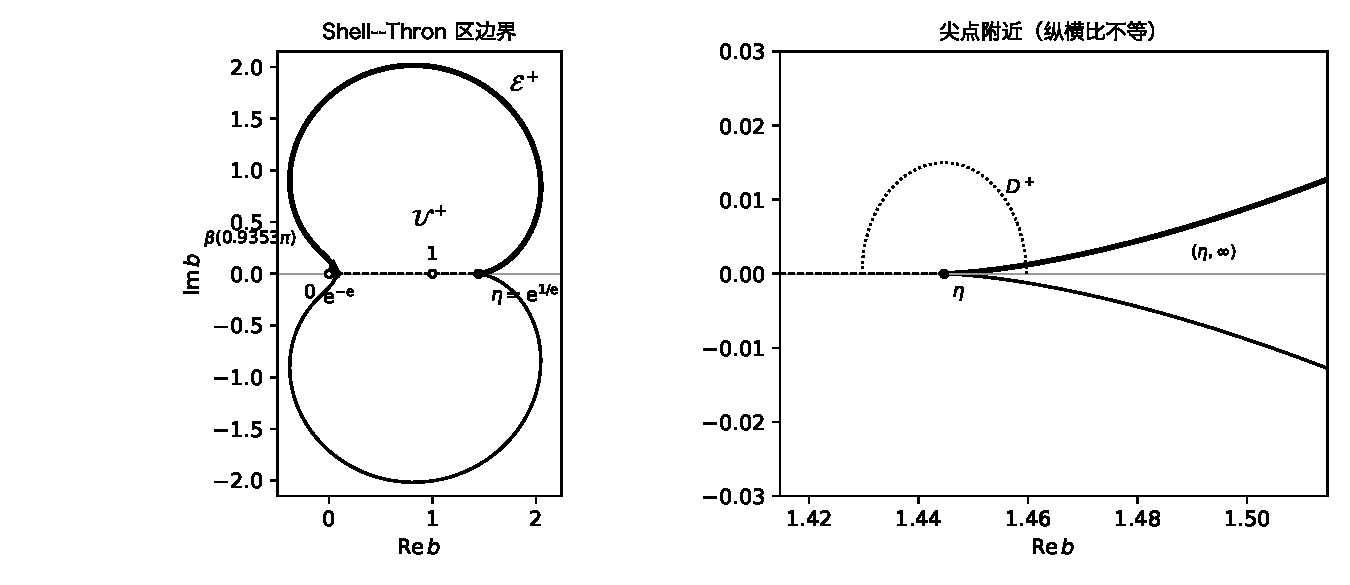
\includegraphics[width=\textwidth]{figures/fig10_shell_thron.pdf}
\caption{Shell--Thron 区的边界 $\beta(\alpha)$（粗线为上中性弧 $0<\alpha<\pi$），实段 $[\ee^{-\ee},\eta]$（虚线），
奇点 $0$、$1$（空心点），以及 \cref{ch10:thm:far-arc} 中的 $\beta(0.9353\pi)$。右图放大尖点 $\eta$ 附近，
外侧实射线 $(\eta,\infty)$ 夹在两条边界弧形成的细角中，虚线半圆是 \cref{thm:cusp} 中的 $D^+$。
脚本 \texttt{figures/fig10\_shell\_thron.py}。}
\label{ch10:fig:shell-thron}
\end{figure}

\Cref{ch10:fig:shell-thron} 中有以下几个特殊点和实段。
\begin{itemize}
\item \textbf{尖点} $\eta=\beta(0)$，乘子 $1$：鞍结点。
\item 实段 $(1,\eta)$：两个实不动点，吸引的乘子 $\lambda_1\in(0,1)$，排斥的 $\lambda_2>1$。这是第 4--9 章的 $s>0$ 一侧。
\item 外侧实射线 $(\eta,\infty)$：共轭排斥不动点对，Kneser 解所在之处。
\item 实段 $(\ee^{-\ee},1)$：吸引不动点的乘子 $\lambda\in(-1,0)$。
\item \textbf{端点} $\ee^{-\ee}=\beta(\pi)$：乘子 $-1$，倍周期分岔点。
\item 实段 $(0,\ee^{-\ee})$：吸引的二周期轨道。
\item $b=1=b(0)$：$E_1\equiv1$，乘子 $0$。它在 $\STreg$ 内部，但如下所述是 Kneser 族的奇点。
\item $b=0$：边界外的极限点，也是奇点。
\end{itemize}

\subsection{尖点}

在 $\eta$ 附近用复参数 $\varepsilon=1-\lambda_1$（本章专用，见记号表）。由 \cref{ch10:lem:param}，
\begin{equation}\label{ch10:eq:cusp-param}
  \log b(\varepsilon)=(1-\varepsilon)\ee^{\varepsilon-1},\qquad
  \log b-\log\eta=-\frac{1}{2\ee}\,\psi_0(\varepsilon)^2,\quad \psi_0(\varepsilon)=\varepsilon(1+O(\varepsilon)) .
\end{equation}
所以 $\varepsilon\mapsto b$ 在 $0$ 附近是 $2:1$ 的。三条曲线在 $\varepsilon$ 平面中的样子是：
\begin{itemize}
\item 实 $b<\eta$：$\varepsilon>0$ 实；
\item 实 $b>\eta$：$\varepsilon(\theta)=1-\theta\cot\theta-\ii\theta=\tfrac13\theta^2-\ii\theta+O(\theta^4)$，$\theta>0$ 小；
\item 上中性弧：$\varepsilon=1-\ee^{\ii\phi}=-\ii\phi+O(\phi^2)$，$\phi>0$ 小，这时 $b-\eta$ 是 $-\varepsilon^2=\phi^2+\ii\phi^3+O(\phi^4)$ 的正倍数。
\end{itemize}
因此上半圆盘 $D^+=\{|b-\eta|<r,\ \Ima b>0\}$ 连同两侧的实段，是 $\varepsilon$ 平面中一个扇形
\[
  \mathcal S_r=\Bigl\{0<|\varepsilon|<r,\ -\tfrac{7\pi}{12}<\arg\varepsilon<\tfrac{\pi}{12}\Bigr\}
\]
的像的一部分（\cite[引理~10.1]{KneserPaper}）。记 $\mathcal S'_r\subset\mathcal S_r$ 为把两条边界射线各向内收 $\tfrac1{10}$ 弧度所得的子扇形；
族建在 $\mathcal S'_r$ 上，使得下面第 6 步中参数圆盘仍留在 $\mathcal S_r$ 内。由于 $b-\eta=-\frac{\eta}{2\ee}\psi_0(\varepsilon)^2\bigl(1+O(\varepsilon^2)\bigr)$，
在 $b$ 平面中经上半圆盘从外侧实射线走到内侧实段（绕尖点转过角度 $\pi$），在 $\varepsilon$ 平面中变成在扇形中从
$\arg\varepsilon\approx-\pi/2$（外侧实射线）转到 $\arg\varepsilon=0$（内侧实段），途中经过 $\arg\varepsilon\approx-\pi/2$ 附近的中性弧。
外侧实射线与中性弧在 $\varepsilon$ 平面中只差 $O(\theta^2)$，这对应图中的细角。

\begin{example}[底数平面的几个数值]\label{ch10:ex:base-numbers}
脚本 \texttt{figures/fig10\_shell\_thron.py}（mpmath，30 位）给出
\[
\begin{gathered}
  \eta=1.44466786100976613\ldots,\qquad \ee^{-\ee}=0.0659880358453125\ldots,\\
  \beta(\tfrac\pi4)=1.63364638222+0.06303054219\,\ii,\qquad
  \beta(\tfrac\pi2)=1.98933207608+1.19328219947\,\ii,\\
  \beta(0.9353\pi)=0.04308627075+0.07503244068\,\ii .
\end{gathered}
\]
论文 11.5 节数值检验的边界点 $\alpha=2\pi(\sqrt2-1)/5$ 是 $b_c=1.52167792861+0.01481787639\,\ii$。
\Cref{ch10:sec:upper} 的直弦参数 $\theta$ 满足 $\theta\cot\theta+\ii\theta=-1$ 的根是
\[
  \theta_*=2.29857900665128663858+0.76604606099318995273\,\ii ,
\]
并且 $b(\theta_*)=\ee^{-\ee}$；
它与论文附录 A.2 的区间证书所验证的根一致。
\end{example}

\subsection{$b=1$ 与 $b=0$ 处的障碍}

\begin{proposition}[{\cite[命题~10.46]{KneserPaper}}]\label{ch10:prop:obstruction}
设 $W\subset\C$ 是连通区域，$0\in W$，$W+1\subset W$。
\begin{enumerate}
\item 不存在在 $W$ 与 $b=1$ 的某个圆盘之积上联合全纯、满足 $F(b,0)=1$ 与 $F(b,z+1)=\exp(F(b,z)\Log b)$ 的族。
\item 对任何在上半平面底数上满足同样条件、且 $b\to0$ 的族，$F(b,2)$ 不能全纯延拓过 $b=0$。
\end{enumerate}
\end{proposition}

\begin{proof}
(1) 若可以，则在 $b=1$ 处 $F(1,z+1)=1$ 对 $z\in W$ 成立。$W+1$ 是 $W$ 的非空开子集，由恒等定理 $F(1,\cdot)\equiv1$。
令 $H(z)=\partial_bF(1,z)$。对函数方程在 $b=1$ 处关于 $b$ 求导：
$\partial_bF(b,z+1)=\exp(F\Log b)\,(\partial_bF\cdot\Log b+F/b)$，在 $b=1$ 处得 $H(z+1)=F(1,z)=1$。
再用恒等定理，$H\equiv1$；但 $F(b,0)=1$ 给出 $H(0)=0$，矛盾。

(2) 由函数方程与归一化，$F(b,1)=b$，$F(b,2)=\exp(b\Log b)$。沿 $b=\ii t$，$t\downarrow0$，这个值趋于 $1$，
而它的导数 $\exp(b\Log b)(1+\Log b)$ 无界。
\end{proof}

\begin{remark}[Paulsen 的唯一性命题]\label{ch10:rem:paulsen}
\cite{Paulsen2019} 把底数延拓族定义为 Kneser 解从 $(\eta,\infty)$ 出发沿 $b$ 的解析延拓。
其命题 2 断言：在 $\Rea z>-2$ 上解析、$F(0)=1$、在 $\pm\ii\infty$ 处趋于两个不动点的解是唯一的。
按原陈述，这对每个实 $b>\eta$ 都不成立：平移 $F_k(z)=\Kkn_b(z+z_k+2)$
给出无穷多个反例~\cite[注~1.2]{KneserPaper}；这里 $z_k$ 是非实点，满足 $E_b(\Kkn_b(z_k))=2\pi\ii k/\log b$，从而 $E_b^2(\Kkn_b(z_k))=1$。Paulsen 与 Cowgill 的唯一性定理~\cite{PaulsenCowgill2017}
不受影响，因为它还要求在 $\C\setminus(-\infty,-2]$ 上解析且实对称。对复底数需要补一个选根条件；
\cref{def:class} 的缝口高度条件就是这样一个条件。
\end{remark}

% ======================================================================
\section{绕过尖点}\label{ch10:sec:cusp}

本节陈述第一个整体定理，并说明它的证明结构。记 $W_0=\{z:\operatorname{dist}(z,[0,1])<\tfrac14\}$。
在 $b<\eta$ 一侧，第 6 章的缝合解 $\Ksew_b$（\cref{thm:sewing}）对实 $b$ 有定义，并且对 $b$ 全纯地延拓到 $(1,\eta)$ 的
一个复邻域 $N_W$（\cite[命题~3.5]{KneserPaper}；$N_W$ 的宽度没有定量）。

\begin{theorem}[绕过尖点的延拓；{\cite[定理~10.14]{KneserPaper}}]\label{thm:cusp}
存在 $r_5>0$ 和开集 $\Omega\supset D^+\cup(\eta-r_5,\eta)\cup(\eta,\eta+r_5)$，其中
$D^+=\{b:|b-\eta|<r_5,\ \Ima b>0\}$，使得以下成立。
\begin{enumerate}
\item Kneser 解 $\Kkn_b$（$b\in(\eta,\eta+r_5)$）沿底数解析延拓为 $\Omega$ 上的族，它在 $\Omega\times W_0$ 上关于 $(b,z)$ 联合全纯。
  特别地，它跨过 $D^+$ 中的 Shell--Thron 边界弧，与该处中性乘子的算术性质无关。
\item 在 $(\eta-r_5,\eta)$ 上，延拓族在 $W_0$ 上等于 $\Ksew_b$。
\item 对每个 $b\in(1,\eta)$，若 $\Kkn_{b+\ii y}$ 先经 $D^+$、再在 $N_W\cap\{\Ima b>0\}$ 内延拓，
  则极限 $\lim_{y\downarrow0}\Kkn_{b+\ii y}$ 在 $z=0$ 附近存在且等于 $\Ksew_b$；由函数方程，它在 $\Ksew_b$ 的整个正则区域上等于 $\Ksew_b$。
\end{enumerate}
\end{theorem}

把 \cref{thm:cusp} 与第 6--8 章的结果合起来，得到 Kneser 解的分离系数的极限。

\begin{corollary}[{\cite[推论~10.15]{KneserPaper}}]\label{ch10:cor:separation}
对 $b\in(1,\eta)$，边界值 $\lim_{y\downarrow0}\Kkn_{b+\ii y}$ 存在且等于 $\Ksew_b$。它的分离系数满足
$c_n/\Lam^n\to B_n\ee^{2\pi\ii na}$（$b\to\eta^-$，每个 $n\ge1$），特别地 $|c_1|/\Lam\to|B_1|=0.0890584\ldots>0$。
\end{corollary}

\begin{proof}
\cref{thm:cusp} 给出边界值等于 $\Ksew_b$；再用 \cref{thm:sewing}（$|c_n/\Lam^n-\tau_n|\le C_n\Lam$）、
\cref{thm:confluence}（$\tau_n\to B_n\ee^{2\pi\ii na}$）和 \cref{prop:B1-nonzero}。
\end{proof}

这个推论是全书的出发点：数值上看到的「Kneser 解与正则解的差的第一个 Fourier 模，按 $\Lam$ 归一化后趋于常数」，
现在有了证明，并且常数被认出是 $\ee^u-1$ 的逆 horn 映射的第一个系数。

\subsection{证明的结构}

证明分七步。下表列出每一步在论文中的位置（论文第 10.1--10.8 节，约 900 行）。
\begin{center}\small
\begin{tabular}{p{2.3cm}p{8.6cm}p{3.2cm}}
\toprule
步骤 & 内容 & 论文出处\\
\midrule
1. 尖点参数 & $\varepsilon\mapsto b(\varepsilon)$ 在扇形上单射；$f_\varepsilon-\id=(u-u_1)(u-u_2)k_\varepsilon$ & 引理 10.1\\
2. 对数坐标 & $\chi=\log\frac{u-u_1}{u-u_2}$ 中一步是平移 $-\varepsilon(1+O(|u|+|\varepsilon|))$ & 引理 10.2\\
3. 倾斜初始区域 & 可容许直线 $\ell$ 与其像之间的细带；商是 $\C^*$ & 引理 10.3、10.4\\
4. 标记点 & 基点轨道第一次进入细带；倒退回 $w=1$ & 引理 10.5、10.6，定义 10.7\\
5. 换线无关 & 不同可容许直线给出同一个解 & 引理 10.8\\
6. 全纯依赖 & Beltrami 方程，\cref{thm:ahlfors-bers} & 命题 10.9\\
7. 两端 & 外端是 Kneser 的弦；内端是缝合曲面的基本域 & 命题 10.11--10.13，定理 10.14\\
\bottomrule
\end{tabular}
\end{center}

下面逐步说明。本节的常数 $C,c$ 不依赖 $\varepsilon$。

\paragraph{第 1 步：尖点参数。}
对小的复 $\varepsilon$，令 $\lambda_1=1-\varepsilon$，$\lambda_2(\varepsilon)$ 是 $\lambda\ee^{-\lambda}=\log b(\varepsilon)$ 在 $1$ 附近的另一个根，
$\lambda_2=1+\varepsilon+\tfrac23\varepsilon^2+O(\varepsilon^3)$。不动点 $u_j=\ee^{\lambda_j-1}-1$，$u_1-u_2=-2\varepsilon(1+O(\varepsilon))$。
在实 $b>\eta$ 一侧，$\lambda_2=\overline{\lambda_1}$，$u_2=\overline{u_1}$，$u_1$ 是上方的不动点 $L_+$；
在实 $b<\eta$ 一侧，$u_1<0<u_2$ 是吸引与排斥的实不动点。所以 $u_1$ 是同一个不动点沿路径的延拓：
它在外侧是排斥的，穿过中性弧后变成吸引的。由 Weierstrass 预备定理（\cref{thm:weierstrass-prep}），
\[
  f_\varepsilon(u)-u=(u-u_1)(u-u_2)\,k_\varepsilon(u),\qquad |k_\varepsilon-\tfrac12|\le\tfrac14\quad(|u|\le\tfrac12),
\]
$k_\varepsilon$ 对 $(\varepsilon,u)$ 联合全纯。

\paragraph{第 2 步：对数坐标。}
令 $q=(u-u_1)/(u-u_2)$，$\chi=\log q$。$\chi\in2\pi\ii\Z$（称为「洞」）对应 $u=\infty$。
在离洞的距离至少 $\tfrac12$ 的区域 $\mathcal G$ 上，$u(\chi)=O(|\varepsilon|)$，所以整个 $\chi$ 平面（除去洞附近）
都被压缩到 $u=0$ 的一个 $O(|\varepsilon|)$ 邻域中。在 $\chi$ 坐标中 $f_\varepsilon$ 是
\[
  f_\chi(\chi)=\chi+\Delta(\chi),\qquad \Delta=-\varepsilon(1+\vartheta),\quad |\vartheta|\le C|\varepsilon|,\quad |\partial_\chi\Delta|\le C|\varepsilon|^2
  \quad(\chi\in\mathcal G)
\]
（\cite[引理~10.2]{KneserPaper}）。也就是说，在 $\chi$ 坐标中映射几乎是平移 $-\varepsilon$，相对误差 $O(|\varepsilon|)$，
并且在两端精确地趋于 $\Log\lambda_1$ 与 $-\Log\lambda_2$。再令 $Z=A_1\chi$，$A_1=1/\Log\lambda_1=-\varepsilon^{-1}(1+O(\varepsilon))$，
则一步是 $Z\mapsto Z+1+O(|\varepsilon|)$。这是第 7 章模型时间 $\Psi_s=A_1\log(u-u_1)+A_2\log(u-u_2)$ 的复参数版本（$A_1\chi$ 是它的主部）。

\paragraph{第 3 步：倾斜初始区域。}
令 $\omega=\ee^{\ii\alpha}$，$x_0\in[-\tfrac12,\tfrac12]$，直线 $\ell=\{\ii\pi+x_0+t\omega:t\in\R\}$。称 $\ell$ 对 $\varepsilon$ \textbf{可容许}，若
\begin{equation}\label{ch10:eq:admissible}
  \cos\alpha\ge\tfrac35,\qquad -\Ima(\varepsilon\bar\omega)\ge\tfrac12|\varepsilon| .
\end{equation}
第二个条件说：一步 $\Delta\approx-\varepsilon$ 有一个确定符号的法向分量，大小在 $[\tfrac25|\varepsilon|,\tfrac65|\varepsilon|]$ 中。
于是 $\ell$ 与 $f_\chi(\ell)$ 之间是宽为 $O(|\varepsilon|)$ 的细带 $\hat H$，它在 $u$ 平面中的像 $H^\ell_\varepsilon$ 连同 $u_1,u_2$ 是一个 Jordan 区域，
由弧 $\gamma=u(\ell)$ 与 $f(\gamma)$ 围成（\cite[引理~10.3]{KneserPaper}）。这就是\textbf{倾斜初始区域}（tilted initial region）。
\begin{itemize}
\item 在外侧实射线上（$\varepsilon=\varepsilon(\theta)$），$\alpha=0$ 可容许，$\chi\in\ii\pi+\R$ 意味着 $q<0$，即 $u$ 在 $u_1$ 与 $u_2=\overline{u_1}$ 之间的线段上：
  $\gamma$ 恰是 Kneser 的弦，$H^\ell_\varepsilon$ 恰是 Kneser 的初始区域~\eqref{ch10:eq:initial-region}。
\item 在内侧实段上（$\varepsilon>0$），$\alpha=\tfrac\pi4$ 可容许，$\alpha=0$ 不可容许（$\Ima\varepsilon=0$）。
\item 沿路径取 $\alpha(\varepsilon)=\tfrac12(\arg\varepsilon+\tfrac\pi2)$，从 $0$ 连续地转到 $\tfrac\pi4$。
\end{itemize}
初始区域就是这样被「倾斜」过去的。当 $\alpha\neq0$ 时 $H^\ell_\varepsilon$ 绕着 $u_1$ 与 $u_2$ 旋转成螺线形。

把 $\gamma$ 上的点与它在 $f(\gamma)$ 上的像粘合，得到 Riemann 曲面 $\Sigma^\ell_\varepsilon$。关键估计是：

\begin{lemma}[平坦模型；{\cite[引理~10.4]{KneserPaper}}]\label{ch10:lem:flat}
设 $\ell$ 对 $\varepsilon\in\mathcal S_{r_0}$ 可容许。在 $Z$ 坐标中，直带 $\hat H_0$（$A_1\ell$ 与 $A_1\ell+1$ 之间）模去 $\zeta\sim\zeta+1$ 是 $\C/\Z$。
映射 $\mathcal H(A_1(\ii\pi+x_0+t\omega)+\mathsf r)=A_1\bigl(\ii\pi+x_0+t\omega+\mathsf r\Delta(\ii\pi+x_0+t\omega)\bigr)$（$0\le\mathsf r\le1$）
诱导拟共形同胚 $\C/\Z\to\Sigma^\ell_\varepsilon$，$|\mathcal H(\zeta)-\zeta|\le C|\varepsilon|$，Beltrami 系数 $|\upsilon_{\mathcal H}|\le C|\varepsilon|$。
因此 $\Sigma^\ell_\varepsilon\cong\C^*$，两端（$u_1$ 端与 $u_2$ 端）对应两个穿孔。
\end{lemma}

这一步解释了为什么中性乘子不构成障碍。经典的做法是用两端的 Koenigs 坐标作穿孔坐标（\cref{ch10:prop:exterior-real} 就是这样做的），
这在乘子为中性时失效：Cremer 点没有线性化，Siegel 点的线性化不提供穿孔坐标。
这里两端是穿孔这件事，是由拟共形映射保持环形端的无穷模推出的~\cite{LehtoVirtanen}，
只用到一步估计 $A_1\Delta=1+O(|\varepsilon|)$ 和横截性 $\Ima(\Log\lambda_1\bar\omega)>0$。
不需要 Brjuno 条件，也不需要 Siegel 圆盘估计。

\paragraph{第 4 步：标记点与归一化。}
基点轨道 $\ustar_n=f^n_\varepsilon(\ustar)$ 在 $\varepsilon=0$ 时沿负实轴单调趋于 $0$，$f_0^n(\ustar)=-2/n+O(\log n/n^2)$。
在 $Z$ 坐标中它每步大约前进 $1$，法向坐标严格增加；它第一次进入细带 $\hat H$ 的点 $\chi^*_{n_0}$ 称为\textbf{标记点}
（\cite[引理~10.5]{KneserPaper}）。由 \cref{ch10:lem:flat} 的定量形式（\cite[引理~10.4(2)]{KneserPaper}），在标记点附近单值化坐标与 $Z$ 相差 $O(|\varepsilon|)$；
用 $f_\varepsilon$ 的主值逆分支沿轨道倒退 $n_0$ 步回到 $\ustar$（\cite[引理~10.6]{KneserPaper}），得到在 $W_0$ 上全纯的
\textbf{归一化倾斜解} $F^\ell_\varepsilon$，$F^\ell_\varepsilon(0)=\ustar$（即 $w=1$），$F(z+1)=f_\varepsilon(F(z))$（\cite[定义~10.7]{KneserPaper}）。
物理点 $\ustar_n$ 可能多次落在螺线形的 $H^\ell_\varepsilon$ 中；只用第一次穿越。其余的穿越对应 \cref{def:class} 之后讨论的平移伪解。

\paragraph{第 5 步：换线无关。}
若 $\ell,\ell'$ 对同一个 $\varepsilon$ 可容许，则 $F^\ell_\varepsilon=F^{\ell'}_\varepsilon$（\cite[引理~10.8]{KneserPaper}）。
证明：每次作用 $f_\chi^{\pm1}$ 使相对于 $\ell'$ 的法向坐标单调变化至少 $\tfrac25|\varepsilon|$，所以 $\hat H$ 中每个点的轨道恰有一个点落在 $\hat H'$ 中；
这给出 $\Sigma^\ell\to\Sigma^{\ell'}$ 的双全纯映射，保持两端，并把标记点送到标记点。

\paragraph{第 6 步：全纯依赖。}
在 \cref{ch10:prop:exterior-real} 中，参数依赖来自 Fischer--Grauert 局部平凡性，那里需要两端有全纯的穿孔坐标。
在中性参数处没有这样的坐标，所以改用 Beltrami 方程。固定 $\varepsilon_0$ 与一条对其邻域内所有 $\varepsilon$ 都可容许的直线 $\ell$，
映射 $\mathcal J_\varepsilon=M_\varepsilon\circ M_{\varepsilon_0}^{-1}:\hat H_{\varepsilon_0}\to\hat H_\varepsilon$ 与粘合相容，其 Beltrami 系数 $\upsilon_\varepsilon$ 满足 $|\upsilon_\varepsilon|\le\tfrac1{10}$，
并且在每点对 $\varepsilon$ 全纯。由 \cref{thm:ahlfors-bers}，归一化解 $\mathcal W_\varepsilon$ 对 $\varepsilon$ 全纯；
再用一个 $\partial_{\bar\varepsilon}$ 抵消论证（内部 Schauder 估计给出所需的 $C^1$ 正则性~\cite[第~V~章]{AhlforsLectures}），
得到 $(\varepsilon,\chi)\mapsto Z_\varepsilon(\chi)$ 联合全纯，从而 $(\varepsilon,z)\mapsto F_\varepsilon(z)$ 在 $\mathcal S'_{r_3}\times W_0$ 上联合全纯
（\cite[命题~10.9]{KneserPaper}）。

\paragraph{第 7 步：走廊的两端。}
\emph{外端}（\cite[命题~10.12]{KneserPaper}）：在 $\varepsilon(\theta)$ 处取 $\ell=\ii\pi+\R$，倾斜区域就是 Kneser 的初始区域，
标记点是实轨道穿过弦的点，所以 $F_{\varepsilon(\theta)}=\Kkn_{b}$。

\emph{内端}（\cite[命题~10.13]{KneserPaper}）：在实 $\varepsilon>0$ 处取 $\alpha=\tfrac\pi4$。在 $\Sigma$ 上用第 5 章的两个正则解的逆
$r_+=R^{-1}$ 与 $r_-=S^{-1}$ 作坐标（沿轨道的 Koenigs 时间，\cite[引理~10.10]{KneserPaper}）。关键计算是虚部：
从标记点沿细带走到 $(u_1,u_2)$ 中的点 $u_m$，$\Ima\chi$ 从 $0$ 增加到 $\pi$，路径经过下半平面，于是
\[
  \Ima r_+(u_m)=A_1\pi+O(\varepsilon)=-\tfrac h2+O(\varepsilon),
\]
而由 \cref{lem:realT}，$\Ima r_+(u_m)\in-\tfrac h2+h\Z$，所以恰为 $-\tfrac h2$。
这正是 \cref{def:class} 的缝口：$r_+=T\circ r_--\ii h$。于是 $\Theta=r_\pm$ 定义了 $\Sigma$ 到缝合曲面的全纯映射，
它把两端送到两端，并且度数为 $1$，因而是双全纯的。标记点送到吸引时间 $n_0$，所以 $F_\varepsilon=\Ksew_b$。

这里倾斜方向的符号决定了缝合分支：负斜率的直线会经过 $u_1$ 上方，给出共轭分支 $\overline{\Ksew_b(\bar z)}$，
但负斜率在实 $\varepsilon>0$ 处不可容许。所以从上半圆盘绕行选出 $\Ksew_b$，从下半圆盘绕行选出它的反射。

\paragraph{收尾。}
由 \cref{ch10:eq:cusp-param}，$\varepsilon\mapsto b(\varepsilon)$ 把 $\mathcal S'_{r_3}$ 双全纯地映到含 $D^+$ 与两侧实段的开集 $\Omega$；
外端给出 (1) 中的认同，内端给出 (2)，(3) 由 $N_W$ 上缝合族的全纯性和恒等定理推出。

\begin{remark}[没有断言的内容；{\cite[注~10.16]{KneserPaper}}]\label{ch10:rem:cusp-scope}
(1) 经下半圆盘延拓得到反射分支 $\overline{\Ksew_b(\bar z)}$。两个分支在某个实高度处至少相差 $2c\Lam$（论文推论 10.49、10.51），
这是 Kneser 族绕 $\eta$ 的单值性（monodromy）。
(2) 定理断言的是 $(b,z)$ 在 $[0,1]$ 附近的全纯性，以及经函数方程到达的正则区域；
对中性参数处 $\Ima z\to\pm\infty$ 时解的行为不作任何断言。
\end{remark}

\subsection{整个上半 Shell--Thron 区}\label{ch10:sec:global}

\cref{thm:cusp} 只在尖点附近的走廊中延拓。下一步把它推到整个 $\Uup$。

\begin{proposition}[{\cite[定理~10.22]{KneserPaper}}]\label{ch10:prop:global}
从 $(\eta,\eta+r_5)$ 出发、经 $\Omega\cap\Uup$ 的 Kneser 解，沿 $\Uup$ 中的每条路径解析延拓，
得到 $z=0$ 处的芽的单值族，关于 $(b,z)$ 联合全纯。对每个 $b_0\in(1,\eta)$，沿 $\Uup$ 中任何趋于 $b_0$ 的路径，
这些芽在 $z=0$ 的某个固定圆盘上一致收敛到 $\Ksew_{b_0}$。
\end{proposition}

证明的工具是\textbf{动力学的拟共形输运}。在乘子平面中固定一个基参数 $\lambda_0$，记 $\sigma_0$ 为吸引不动点处的 Koenigs 坐标，
$\mathfrak s=\Log\lambda$，$\mathfrak s_0=\Log\lambda_0$。在吸引域 $B_0$ 上取 Beltrami 系数
\[
  \nu_\lambda=\mathsf c(\lambda)\,\frac{\sigma_0}{\overline{\sigma_0}}\,\frac{\overline{\sigma_0'}}{\sigma_0'},\qquad
  \mathsf c(\lambda)=\frac{\mathfrak s-\mathfrak s_0}{\mathfrak s+\overline{\mathfrak s_0}},\quad |\mathsf c|<1,
\]
在 $B_0$ 外取 $0$。它是 $E_0$ 不变的，并且对 $\lambda$ 全纯。由 \cref{thm:ahlfors-bers} 得到的归一化解 $\mathcal Q_\lambda$
满足 $\mathcal Q_\lambda\circ E_0=E_\lambda\circ\mathcal Q_\lambda$（\cite[命题~10.18]{KneserPaper}）：$\mathcal Q_\lambda E_0\mathcal Q_\lambda^{-1}$ 的伸缩为零，
是 $\C$ 上覆盖 $\C^*$ 的整函数，所以形如 $\ee^{Aw}$，乘子条件迫使 $A=\lambda\ee^{-\lambda}$。
把一个倾斜初始区域用 $\mathcal Q_\lambda$ 搬过去，就得到对所有 $\lambda\in\D\cap\HH$ 由同一个公式定义的族 $\Ftr$（输运族），
它自动是单值的（\cite[命题~10.19]{KneserPaper}）。剩下的工作是比较引理：在 $\lambda_0$ 附近 $\Ftr$ 与尖点族一致（\cite[引理~10.21]{KneserPaper}）。
这需要控制 $\mathcal Q_\lambda$ 在两端的提升（\cite[引理~10.20]{KneserPaper}），是这一节技术上最细的部分。

\begin{remark}[穿孔内部；{\cite[注~10.24]{KneserPaper}}]\label{ch10:rem:punctured}
上面的构造只用到 $\Rea\mathfrak s<0$，所以 $\mathfrak s\mapsto\Ftr_{\mathfrak s}$ 在整个左半平面上单值全纯。
左半平面是 $\STreg^\circ\setminus\{1\}$ 的万有覆盖。因此 Kneser 族沿 $\STreg^\circ\setminus\{1\}$ 中每条路径都可延拓，
绕 $b=1$ 的单值性作用为 $\mathfrak s\mapsto\mathfrak s+2\pi\ii$。这个单值性是否平凡，是开放问题（\cref{ch:open}）。
数值上，边界值 $\Ksew_b$ 的 $|c_1|/\Lam$ 在 $b\downarrow1$ 时停在 $0.08$ 附近（$b=1.01$ 时为 $0.0816$），而 $\Lam\to1$。
\end{remark}

% ======================================================================
\section{整个上半平面}\label{ch10:sec:upper}

\begin{theorem}[整个上半平面；计算机辅助；{\cite[主定理~E、定理~10.40]{KneserPaper}}]\label{thm:upper-half-plane}
Kneser 解 $\Kkn_b$（$b>\eta$）沿上半平面 $\HH=\{\Ima b>0\}$ 中每条路径（取主值 $\Log b$）解析延拓。
\begin{enumerate}
\item 结果是 $z=0$ 处的芽的单值族，关于 $(b,z)$ 联合全纯。在 $\Eup=\HH\setminus\overline{\STreg}$ 上它由直弦加标记点的构造给出，
  在 $\Uup$ 上由输运族 $\Ftr$ 给出，并且全纯地跨过整条开上中性弧 $\{\beta(\alpha):0<\alpha<\pi\}$。
\item 它在 $(1,\eta)$ 上的边界值是 $\Ksew_b$，与 $\HH$ 中所用的路径无关。
\item 它全纯地延拓到实段 $[\exp(-12\ee^{12}),\exp(-\tfrac15\ee^{1/5})]\approx[\ee^{-1.95\cdot10^6},0.7833]$ 的一个邻域，
  这个实段含端点 $\ee^{-\ee}$。
\item 它全纯地跨过 $(0,\eta)\setminus\{1\}$ 的每一点；$b=0$ 与 $b=1$ 是 \cref{ch10:prop:obstruction} 意义下的真奇点。
\item 若把 \cite{Paulsen2019} 的族按其定义理解为 Kneser 解沿上半平面路径（主值对数）的解析延拓，则它就是这个族。
\item 经下半平面的延拓是复共轭族。
\end{enumerate}
\end{theorem}

\paragraph{状态。}
(1)--(3)、(5) 用到区间算术证书（证·机）；(4) 中 $(1,\eta)$ 与 $(\ee^{-\ee},1)$ 的部分以及奇点的断言是纸面证明，
$(0,\ee^{-\ee})$ 的部分把纸面论证锚定在 (3) 的证书区间中的一点上。
论文中的对应：(1) 是定理 10.33、10.34、10.40 与推论 10.35；(2) 是 \cref{ch10:prop:global}；(3) 是定理 10.43；
(4) 是定理 10.45 与命题 10.46；(5) 是推论 10.41。

\subsection{直弦加标记点}

远离尖点时，两个不动点相距不小，倾斜区域的估计（以 $|\varepsilon|$ 小为前提）不再可用。
这时用回 Kneser 自己的直弦，只是参数变成复的。对复数 $\theta$，$0<\Rea\theta<\pi$，令
\[
  \mu=\theta\cot\theta,\quad \lambda_\pm=\mu\pm\ii\theta,\quad r=\ee^{\mu},\quad
  \log b=\frac{\theta\ee^{-\mu}}{\sin\theta},
\]
则 $L_\pm=r\ee^{\pm\ii\theta}$ 是 $E_b(w)=\ee^{w\log b}$ 的不动点，乘子为 $\lambda_\pm$，且 $\log b=\lambda_+\ee^{-\lambda_+}$。
实 $\theta\in(0,\pi)$ 给出外侧实射线。仿射坐标
\[
  \zeta(w)=\frac{w/r-\cos\theta}{\ii\sin\theta}
\]
把 $L_\pm$ 送到 $\pm1$，把弦送到 $[-1,1]$，并把 $E_b$ 共轭为整函数
\begin{equation}\label{ch10:eq:seam-map}
  \mathsf s_\theta(\zeta)=\frac{\ee^{\ii\theta\zeta}-\cos\theta}{\ii\sin\theta},\qquad \mathsf s_\theta(\pm1)=\pm1,\quad \mathsf s_\theta'(\pm1)=\lambda_\pm .
\end{equation}
令 $k_\theta(t)=(\mathsf s_\theta(t)-t)/(1-t^2)$，它对 $t$ 是整函数。

\begin{lemma}[月牙形；{\cite[引理~10.27、10.38]{KneserPaper}}]\label{ch10:lem:crescent}
若对 $-1<t<1$ 有
\begin{equation}\label{ch10:eq:crescent-ineq}
  \Ima k_\theta(t)<0,\qquad \Ima\bigl(\overline{\mathsf s_\theta'(t)}\,k_\theta(t)\bigr)<0,
\end{equation}
且 $\Ima\lambda_+>0>\Ima\lambda_-$，则 $A_\theta=\mathsf s_\theta([-1,1])$ 是从 $-1$ 到 $1$ 的简单弧，除端点外在开下半平面中；
$[-1,1]\cup A_\theta$ 围出 Jordan 区域 $H_\theta$；$N_\theta(t,\sigma)=t+\sigma(\mathsf s_\theta(t)-t)$ 是 $(-1,1)\times[0,1]$ 到 $H_\theta\setminus\{\pm1\}$ 的实解析微分同胚；
粘合 $t\sim\mathsf s_\theta(t)$ 得到的曲面拟共形于 $\C/\ii\Z$，Beltrami 系数对 $\theta$ 全纯，因而它双全纯于 $\C^*$。
\end{lemma}

不等式~\eqref{ch10:eq:crescent-ineq} 的第一条说像弧在弦的下方，第二条说插值 $N_\theta$ 的 Jacobian 不变号。
它们都是关于一个实变量 $t\in[-1,1]$ 和复参数 $\theta$ 的严格不等式，正适合区间算术。

\emph{标记点。}令 $w_{-1}=0$，$w_n=E_b^n(1)$（$n\ge0$），$\zeta_n=\zeta(w_n)$。若 $w_{-1},\dots,w_{n-1}$ 都在弦的上方（$\Ima\zeta>0$），
而 $\zeta_n\in H_\theta\setminus A_\theta$，称 $n$ 为\textbf{进入指标}，$\zeta_n$ 在商曲面中的类为\textbf{标记点}。它是内蕴定义的。
单值化把两端送到 $0,\infty$、标记点送到 $1$，取对数提升并用 $E_b^{-n}$ 沿轨道倒退到 $w_0=1$，得到解 $F^{\mathrm{far}}_\theta$（\cite[定义~10.30]{KneserPaper}）。
对实 $\theta$ 它就是 Kneser 解（\cite[命题~10.32]{KneserPaper}），对 $\theta$ 联合全纯（\cite[命题~10.31]{KneserPaper}）。

于是证明整体结果的任务化为：在所需的参数集上，验证~\eqref{ch10:eq:crescent-ineq} 并找到进入指标。

\begin{theorem}[远离尖点跨过边界；{\cite[定理~10.33、10.34，推论~10.35]{KneserPaper}}]\label{ch10:thm:far-arc}
Kneser 族沿外侧路径到达上中性弧的每一点 $\beta(\alpha)$（$0<\alpha<\pi$），在 $\beta(\alpha)$ 的完整邻域上全纯，
并以芽 $\Ftr$ 进入 $\Uup$。对 $\alpha\le0.9353\ldots\pi$ 用参数区域上的证书 \texttt{certify\_far\_collar.py}，
对 $0.935\pi\le\alpha<\pi$ 用 \texttt{certify\_last\_boundary\_arc.py}。端点 $\beta(\pi)=\ee^{-\ee}$ 单独处理。
\end{theorem}

\subsection{外部区域}

在 $\Eup$ 上所有不动点都排斥，$\Eup$ 单连通，从外侧实射线延拓来的不动点 $L_+$ 单值，
其乘子 $\lambda(b)$ 把 $\Eup$ 双全纯地映到一个区域 $\mathcal V$，逆为 $\lambda\mapsto\exp(\lambda\ee^{-\lambda})$（\cite[引理~10.37]{KneserPaper}）。
对 $\lambda\in\mathcal V$，令 $\theta(\lambda)\neq0$ 是 $(\lambda-2\ii\theta)\ee^{2\ii\theta}=\lambda$ 的根；这等价于 $\lambda_+(\theta)=\lambda$，
而 $\lambda-2\ii\theta$ 是另一个不动点 $L_-=\ee^{\lambda-2\ii\theta}$ 的乘子。于是直弦构造对每个 $b\in\Eup$ 都有定义，
问题只是 $\theta(\lambda)$ 能否连续选取、以及月牙不等式与进入指标是否处处成立。
论文的命题 10.39 用一个证书回答了这个问题。

\subsection{区间证书检查什么}\label{ch10:sec:certificates}

全部证书都是用 python-flint/Arb~\cite{Johansson2017Arb} 球算术写的 Python 程序，外向舍入，每个严格不等式都在包络上判定；浮点只用来选 Krawczyk 盒的中心。
Krawczyk~\cite{Krawczyk1969} 算子
\[
  K=m-Yf(m)+\bigl(1-Yf'(B)\bigr)(B-m),\qquad K\subset\operatorname{int}B
\]
证明 $f$ 在盒 $B$ 中对给定球中的每个参数都有唯一零点（判据的陈述与证明梗概见 \cref{app:tools}）。各证书的内容如下（论文附录 A）。
\begin{itemize}
\item \texttt{certify\_far\_collar.py}（A.1，约 6 分钟，33\,027 个盒）。参数区域 $\Theta=\Theta_{\mathrm C}\cup\Theta_{\mathrm K}$ 由尖点处的锥和一块弯曲区域组成。
  在其上验证~\eqref{ch10:eq:crescent-ineq}、$|\lambda_+|$ 沿竖直纤维单调减并在顶边小于 $1$（所以每条竖直路径恰好穿过中性弧一次）、
  以及沿轨道的进入指标：要么 Krawczyk 检验证明 $\zeta_n=N_\theta(t,\sigma)$，$|t|<1$，$0<\sigma<1$；要么 $\zeta_n$ 落在一个矩形中，
  该矩形的下半部分与 $\mathsf s_\theta$ 作用后的上半部分都被证明在 $H_\theta$ 中。在锥上用解析估计代替逐盒验证（\cite[引理~10.28]{KneserPaper}）。
\item \texttt{certify\_last\_boundary\_arc.py}（A.2）。验证 $\lambda_+(\theta)=-1$ 的简单根 $\theta_*$（\cref{ch10:ex:base-numbers}）；
  在矩形 $[2.19,2.31]+\ii[0.71,0.78]$ 上验证 $\Rea(\lambda_+'(\theta)/\lambda_+'(\theta_*))>\tfrac45$，由 Noshiro--Warschawski 判据（\cref{app:tools}）
  $\lambda_+$ 在其上单射；用压缩盒得到逆分支 $\theta(\alpha)$。月牙不等式在 $[-1,\tfrac{19}{20}]$ 上直接验证，在 $[\tfrac{19}{20},1]$ 上验证导数为正，
  并用端点处的精确恒等式 $f_1(1)=f_2(1)=-\tfrac12\sin\alpha$ 闭合到 $t=1$。进入指标恒为 $-1$：$\zeta(0)=\ii\cot\theta\in\operatorname{int}H_\theta$。
\item \texttt{certify\_upper\_halfplane.py}（A.3，约 15 分钟）。四部分：(T) 尾部 $\Rea\lambda\le-12$，用 $\mathsf w=1/\lambda$ 的压缩映射定根，6\,230 个盒；
  (K) 核心 $-12\le\Rea\lambda\le5$，$|\lambda-1|\ge0.08$，丢弃确定不在 $\mathcal V$ 中的盒（用 $\phi(\D)$ 的星形边界），在其余盒上用 Krawczyk 定根，
  相邻盒的根用凸包上的唯一性对接；(P) 尖点 $|\lambda-1|<0.08$，用 Rouché 定理（\cref{app:tools}）证明根唯一并落在锥 $\Theta_{\mathrm C}$ 中；
  (I) 接口与锚点：在 $\lambda=\cot1+\ii$ 处的盒包含实根 $\theta=1$，这把整条分支锚定在外侧实射线上。
\item \texttt{certify\_endpoint.py}（A.4，不到 1 分钟）。在 $\ee^{-\ee}$ 附近与实段上，直弦构造在一个对数坐标中验证（论文引理 10.42 的条件 (a)--(f)）。
\end{itemize}
外侧覆盖、尖点与接口合起来证明：$\theta(\lambda)$ 在 $\mathcal V$ 上是一条连续分支，处处满足月牙条件并有进入指标。
再加上 \cref{ch10:thm:far-arc} 和 \cref{ch10:prop:global}，三块（$\Eup$、开中性弧、$\Uup$）在重叠处一致，
$\HH$ 单连通，所以延拓与路径无关。这就是 \cref{thm:upper-half-plane}(1)(2)。

\subsection{端点与 $\eta$ 以下的实轴}

\emph{端点。}在 $\ee^{-\ee}$ 附近，伙伴不动点 $L_-$ 不是实的，构造不对共轭对称，所以经上半平面与经下半平面的延拓不必一致。
直弦构造在乘子平面的正方形 $[-1.1,-0.9]\times[-0.1,0.1]$ 和长条 $[-12,-\tfrac15]\times[-10^{-3},10^{-3}]$ 上被验证，标记点为 $w_{-1}=0$
（\cite[定理~10.43]{KneserPaper}）。

\emph{二周期段。}对 $b=\ee^{-\mathcal M}\in(0,\ee^{-\ee})$，实二周期轨道 $p<q$ 的乘子 $m$ 有显式参数化
\[
  \mathcal Mp=u(\coth u-1),\quad \mathcal Mq=u(\coth u+1),\quad \mathcal M=\frac{u}{\sinh u}\ee^{u\coth u},\quad m=\Bigl(\frac{u}{\sinh u}\Bigr)^2,\quad u>0,
\]
$\mathcal M$ 从 $\ee$ 增到 $\infty$，$m$ 从 $1$ 减到 $0$。所以 $m$ 是整段 $(0,\ee^{-\ee})$ 上的实解析坐标。
以二周期的 Koenigs 坐标作输运（与 \cref{ch10:sec:global} 相同的拟共形技术），锚定在证书区间中的 $b_*=\exp(-2\ee^2)$ 处
（\cite[定理~10.45]{KneserPaper}）。

\emph{实段 $(1,\eta)$ 与 $(\ee^{-\ee},1)$。}前者由 \cref{ch10:prop:global} 与缝合族的参数全纯性得到，后者由输运族直接跨过（\cite[命题~10.23]{KneserPaper}）。

\begin{remark}[与 Paulsen 族的关系]\label{ch10:rem:paulsen-family}
\cite{Paulsen2019} 的族由底数上的解析延拓定义，但那里跨过 Shell--Thron 边界只有数值论证（数值格式的连续性）。
\cref{thm:upper-half-plane}(5) 解决了这一点。在 $b=\sqrt2$ 处，缝合方程给出 $\Ima\Ksew_{\sqrt2}(\tfrac12)=-1.18899697185\cdot10^{-48}$，
与 Paulsen 的 120 位计算值 $-1.18899697\cdot10^{-48}$ 在给出的全部 9 位（含符号）上一致~\cite[第~11~节]{KneserPaper}。
这是数值核对，不是证明的一部分。
\end{remark}

% ======================================================================
\section{其他族}\label{ch10:sec:other}

一般理论对下面三个族逐字成立：只需验证 (H1)--(H4)，并对需要 (H5) 的陈述单独处理 $B_1\neq0$。
整体结果（\cref{thm:cusp}、\cref{thm:upper-half-plane} 的类比）则依赖每个族的整体几何。

\subsection{三个族的开折数据}

\begin{example}[$w^2+c$]\label{ch10:ex:quad}
$f_c(w)=w^2+c$ 在 $c=\tfrac14$ 处有二重不动点 $w^*=\tfrac12$。令 $c=\tfrac14-s$，$u=w-\tfrac12$，
则 $f_s(u)=u+u^2-s$：$g(u)=u+u^2$，$a_2=1$，$a_3=0$，$\rho=1$，$X=1$，$\gamma=1$。这是平移开折，所以 $\kappa^{(n)}=\ktr^{(n)}(u+u^2)$。
$s>0$ 时有两个实不动点 $\tfrac12\pm\sqrt s$。基点可取 $w_0=0$、$0.2$、$0.35$ 或 $f_c^3(0)$（在 $c=\tfrac14$ 处为 $\tfrac{89}{256}$）；
它们都满足 (H4)。$B_1\neq0$：直接吸引域中只有一个临界点（\cite[注~9.5]{KneserPaper}）。
\end{example}

\begin{example}[$v-\sin v+c$]\label{ch10:ex:sine}
$f_c(v)=v-\sin v+c$ 的二重不动点要求 $\sin v=c$，$\cos v=0$，取 $v^*=\tfrac\pi2$，$c=1$。令 $c=1-s$，$u=v-\tfrac\pi2$，
则 $f_s(u)=u+1-\cos u-s$：$g(u)=u+\tfrac12u^2-\tfrac1{24}u^4+\cdots$，$a_2=\tfrac12$，$a_3=0$，$\rho=1$，$X=1$，$\gamma=1$。
临界值 $2\pi k+1$ 都是实的，直接吸引域只含 $k=0$ 那一个；但 $f$ 有无穷多个临界值，不是有限型，Chéritat 的单奇值论证能否适用需要核查。
所以 $B_1\neq0$ 的状态是「推导」，(H5) 作为假设保留。
\end{example}

\begin{example}[$w+(w^2-c)\ee^w$]\label{ch10:ex:expq}
$f_c(w)=w+(w^2-c)\ee^w$ 在 $c=0$ 处有二重不动点 $w^*=0$。令 $c=s$，则 $f_s(u)=u+u^2\ee^u-s\ee^u$：
$g(u)=u+u^2+u^3+\cdots$，$a_2=1$，$a_3=1$，$\rho=0$，$X=\ee^u$，$\gamma=1$。$s>0$ 时不动点是 $\pm\sqrt s$，两个乘子 $1\pm2\sqrt s\,\ee^{\pm\sqrt s}$ 不对称。
$B_1\neq0$ 只有数值（$|B_1|\approx2744$）。
\end{example}

\begin{example}[数值比较]\label{ch10:ex:numerics-table}
脚本 \texttt{generality\_check.py}（论文注 9.14）对任意给定 $f$ 及其在不动点处的 Taylor 系数实现第 5--8 章的构造。
下表是 $\lambda_1=0.97$ 处的值（取自 $\lambda_1=0.5,\dots,0.97$ 的扫描）；第四列在 $p\to0$ 时趋于 $\Rea\kappa^{(1)}$。
\begin{center}\small
\begin{tabular}{lllll}
\toprule
族 & $\rho$ & $|B_1|$ & $\Rea\log(\tau_1/B_1\ee^{2\pi\ii a})/p$ & $|\tau_1|/|B_1|-1$\\
\midrule
$b^w$ & $1/3$ & $0.0890584364122$ & $-0.0101990$ & $-9.4\cdot10^{-6}$\\
$w^2+c$ & $1$ & $0.0597942361690$ & $-0.0150481$ & $-1.4\cdot10^{-5}$\\
$v-\sin v+c$ & $1$ & $0.0723786416245$ & $-0.0142133$ & $-1.3\cdot10^{-5}$\\
$w+(w^2-c)\ee^w$ & $0$ & $2744.09379131$ & $+1.08542$ & $+1.0\cdot10^{-3}$\\
\bottomrule
\end{tabular}
\end{center}
在每个族中，$\tau_n$、$t_n/t_1^n$ 与 $\log(\tau_1/B_1\ee^{2\pi\ii a})/p$ 都以 $O(p)$ 的速率收敛；缝口条件 $\Ima t_0=h/2$ 精确到 $10^{-31}$ 以上；
缝合迭代给出 $\hat c_n=\tau_n(1+O(\Lam))$。对 $w^2+c$ 用三个基点 $w_0=0,0.2,0.35$，第四列的实部在显示的 10 位上一致（\cref{prop:base-point}），
虚部则从 $-0.07$ 变到 $116$。$w^2+c$ 的极限值是 $\Rea\ktr^{(1)}(u+u^2)=-0.0150441028391897$（\texttt{kappa\_variation.py}）。
$w^2+c$ 与 $v-\sin v+c$ 的芽有相同的 $\rho$，因而形式共轭，但 $|B_1|$ 不同（数值），所以它们不是实解析共轭的（\cref{cor:invariance}）。
\end{example}

\paragraph{状态。}三个新族上，汇流、缝合解、一阶与全阶展开、基点无关性都是一般定理的特例（已证）；
$B_1\neq0$ 对 $w^2+c$ 已证，对 $v-\sin v+c$ 是推导，对 $w+(w^2-c)\ee^w$ 是数值。
整体延拓：$w^2+c$ 见下一小节；另外两个族\textbf{未检验}。

\subsection{$w^2+c$ 的整体延拓}

对应关系如下。实 $c>\tfrac14$ 时两个不动点 $\tfrac12\pm\ii\sqrt{c-\tfrac14}$ 共轭排斥，实轴逃逸；Shell--Thron 区对应 Mandelbrot 集的主心形区
$\mathcal C=\{\lambda/2-\lambda^2/4:|\lambda|<1\}$；尖点 $\eta$ 对应 $c=\tfrac14$；端点 $\ee^{-\ee}$ 对应 $c=-\tfrac34$（乘子 $-1$）。
归一化取 $F_c(0)=f_c^3(0)$，对应以临界点为标记 $F(-3)=0$。

这个族的直弦几何是精确的，不需要区间算术。设 $c\in\HH$，取全纯平方根 $a(c)$，$a^2=\tfrac14-c$，$\Rea a<0<\Ima a$。
在坐标 $w=\tfrac12+a\zeta$ 中，不动点 $\tfrac12\pm a$ 对应 $\zeta=\pm1$，映射变为
\[
  S_a(\zeta)=\zeta+a(\zeta^2-1).
\]

\begin{proposition}[二次族的直月牙；\texttt{docs/proofs/quadratic-continuation.tex} 定理 1]\label{ch10:prop:quad-crescent}
对每个 $c\in\HH$，弦 $[-1,1]$ 与它的像 $S_a([-1,1])$ 只在端点相交，围出 Jordan 区域 $H_a$，参数化为
$M_a(t,\sigma)=t+\sigma a(t^2-1)$，$-1\le t\le1$，$0\le\sigma\le1$。开区域是凸的，含于 $\Ima\zeta<0$，并且 $S_a$ 在整个下半平面上单射。
\end{proposition}

\begin{proof}
写 $a=r+\ii\beta$，$\beta>0$，引入实线性坐标 $T=\Rea\zeta-(r/\beta)\Ima\zeta$，$Y=\Ima\zeta/\beta$。
对 $\zeta=M_a(t,\sigma)$ 有 $T=t$，$Y=\sigma(t^2-1)$。所以开区域恰是 $\{-1<T<1,\ T^2-1<Y<0\}$，
它是凸函数 $T^2-1$ 的上图与一个半平面之交在可逆线性映射下的像，因而是凸的；两条边界弧的 $T$ 坐标都是 $t$，$Y$ 坐标分别是 $0$ 与 $t^2-1$，
所以它们单射且内部不交。若 $S_a(\zeta)=S_a(\zeta')$，$\zeta\neq\zeta'$，则 $\zeta+\zeta'=-1/a$，其虚部为正；
所以闭下半平面中两点不会碰撞。
\end{proof}

在此基础上，证明稿（\texttt{docs/proofs/quadratic-continuation.tex}，2026-10-04）给出了论文主定理 D、E 的二次族类比的证明：
\begin{itemize}
\item \textbf{二次族 G}（证明稿定理 16，\texttt{thm:G}）：$c>\tfrac14$ 的临界轨道标记的实 Kneser 月牙族在整个 $\HH$ 上有单值全纯延拓，
  在每个 $c_0\in\HH$ 附近由联合全纯的 $F(c,z)$ 表示，$F(c,0)=f_c^3(0)$。
\item \textbf{二次族 F}（证明稿定理 20，\texttt{thm:F}）：该族经 $c=\tfrac14$ 的上方穿孔邻域延拓，跨过中性边界而不需要乘子的算术条件；
  它在每个实 $0<c<\tfrac14$ 处的边界值是由接缝 $T-\ii h$ 指定的缝合解 $\Ksew_c$；它在整个上主心形区中单值。
\end{itemize}
证明的组成：直月牙几何（\cref{ch10:prop:quad-crescent}）；对 $|a|>\tfrac12$，临界值 $c$ 严格位于月牙内部，用作标记（习题~\ref{ch10:ex:quad-mark}）；
$0<|a|\le\tfrac1{16}$ 用解析的首次穿越估计；其余的紧区域 $\tfrac1{16}\le|a|\le\tfrac12$ 用 4\,013 个闭参数盒的 Arb 覆盖
（\texttt{certify\_quad\_entry.py}，最大轨道指标 21），并由独立程序 \texttt{verify\_quad\_entry.py} 以 90 位精度重放、用 282 个有理横向分片验证精确覆盖；
主心形区内用显式的多项式乘子形变输运（从 $\lambda_*=\ii/2$ 出发，主解为奇函数、保持临界点 $0$），并在开重叠集上与直弦族比较；
尖点走廊用倾斜区域，常数由 \texttt{certify\_quad\_geometry.py} 的 14 项 Arb 检查核验。

\paragraph{状态与范围。}二次族 F、G 是\textbf{单独的证明稿}中的结果（作者标为已证 + 证·机），不在投稿论文中，也不由一般理论推出。
证明稿是 2026-10-04 的研究笔记，\textbf{未经同行评审}；本书只转述其结构，不对其正确性背书。
它们用到了二次多项式特有的结构（精确月牙、临界点标记、主心形区的显式输运）。
证明稿不断言在尖点本身、实端点 $c=-\tfrac34$ 处的延拓，也不断言所有参数有一个共同的整体高度定义域。
此前的数值证据（$\theta$ 迭代在 $c$ 平面采样点上的收敛、跨中性带插值、竖直阶梯外推 $\hat c_1$ 与 $\tau_1$ 吻合到 $O(\Lam)$ 修正项本身的 0.3\%）
只是数值，它们并不蕴含证明，证明也不蕴含该数值算法的收敛。

\begin{example}[$\theta$ 迭代的共振障碍]\label{ch10:ex:theta-obstruction}
用两侧 Schröder（Koenigs）表示求值的 $\theta$ 迭代算法，不能在整个 $\HH$ 上收敛。取 $c=\tfrac14+\tfrac\ii2$，
上方不动点 $L=\tfrac\ii2$，乘子 $\lambda=2L=\ii$。逆 Schröder 级数 $u(\zeta)=\sum_{k\ge1}u_k\zeta^k$，$u(\lambda\zeta)=\lambda u(\zeta)+u(\zeta)^2$，
要求
\[
  (\ii^k-\ii)\,u_k=\sum_{j=1}^{k-1}u_ju_{k-j},\qquad u_1=1 .
\]
逐阶解出 $u_2=\tfrac{-1+\ii}2$，$u_3=\tfrac{-1-\ii}2$，$u_4=\tfrac{1-5\ii}4$；到 $k=5$ 左边系数 $\ii^5-\ii=0$，右边却是 $\tfrac{3-5\ii}2\neq0$。
所以形式级数都不存在。更一般地，若 $w^2+c$ 的不动点乘子 $\lambda$ 是 $q$ 次单位根且可线性化，则 $f_c^q$ 在该点附近共轭于恒等映射，
从而 $f_c^q=\id$，与 $\deg f_c^q=2^q$ 矛盾。这样的参数在开中性弧上稠密。
精确有理数验证见 \texttt{certify\_quad\_theta\_obstruction.py}（9 项检查）。这个反例\textbf{不}否定二次族 F、G：
商曲面的构造不需要固定点的线性化（与 \cref{ch10:lem:flat} 后的讨论相同）。
\end{example}

\subsection{什么是一般的，什么是特殊的}

\begin{center}\small
\begin{tabular}{p{4.2cm}p{4.6cm}p{4.2cm}}
\toprule
结果 & 用到族的什么 & 状态\\
\midrule
转移映射、焊接恒等式、缝合解 & 两个实双曲不动点及其间的不变区间 & 一般（已证）\\
汇流、一阶与全阶展开、变分公式 & 抛物芽与开折方向 & 一般（已证）；需 (H5) 的部分见上\\
$B_1\neq0$ & 直接吸引域中只有一个奇异值 & exp、quad 已证；sine 推导；expq 数值\\
绕尖点（\cref{thm:cusp}） & 尖点处二次切；指数族的具体估计 & tetration 已证；quad 单独证明稿（未审稿）；其他未检验\\
全上半平面（\cref{thm:upper-half-plane}） & 指数函数的整体几何 & tetration 证·机；quad 单独证明稿（未审稿）；其他未检验\\
\bottomrule
\end{tabular}
\end{center}
绕尖点的论证只用到尖点附近的局部估计（第 1--6 步）和内端的缝合认同（第 7 步），后者是一般理论的一部分；
外端用到的是「外侧实参数处有一个 Kneser 型构造」。所以 \cref{thm:cusp} 移植到一般开折的障碍主要在外端：
一般的族在尖点的另一侧不一定有共轭不动点对的实构造。这个问题在 \cref{ch:open} 中作为 C3 讨论。

% ======================================================================
\notes

\paragraph{Kneser 与 Shell--Thron。}Kneser 的构造见~\cite{Kneser1950}；其初始区域的表述与唯一性刻画见 Trappmann 与 Kouznetsov~\cite{TrappmannKouznetsov2011}，
高精度算法见~\cite{Kouznetsov2009,KouznetsovTrappmann2010,KouznetsovTrappmann2012}。
Shell--Thron 区得名于 Thron~\cite{Thron1957} 与 Shell~\cite{Shell1962} 关于无穷幂塔收敛的工作。
Paulsen~\cite{Paulsen2019} 提出沿底数延拓 Kneser 解，\cite{PaulsenCowgill2017} 给出实底数 $b>\eta$ 时的唯一性定理，
\cite{Paulsen2026} 研究了 $b\to1$ 时部分非整数高度的行为。Nixon~\cite{Nixon2022} 用无穷复合构造 Shell--Thron 区内部的非正则解，
并用 1-周期的 $\theta$ 映射与正则解比较；这正是本书的分离形式 $K=R\circ(\id+P)$。

\paragraph{与论文的对应。}本章的 \cref{thm:cusp} 是论文主定理 D 的精确形式（论文定理 10.14，标签 \texttt{thm:cusp}）；
\cref{ch10:prop:global} 是论文定理 10.22（\texttt{thm:global}），与定理 10.14 合起来给出主定理 D；\cref{thm:upper-half-plane} 汇总论文主定理 E，
其精确形式分布在定理 10.33（\texttt{thm:far}）、10.34（\texttt{thm:last-arc}）、10.40（\texttt{thm:upper}）、10.43（\texttt{thm:endpoint}）、
10.45（\texttt{thm:positive-real-axis}）、命题 10.46（\texttt{prop:zero-one-obstruction}）与推论 10.41（\texttt{cor:paulsen}）中。
区间证书的说明在论文附录 A.1--A.5。论文的引理编号以 2026-10-07 的 \texttt{main.pdf} 为准。

\paragraph{一般族。}三个新族的数值检验与假设审查见论文第 9 节（注 9.5、9.13、9.14、9.15）。
二次族 F、G 的证明稿 \texttt{docs/proofs/quadratic-continuation.tex} 还包含一个一般的「带标记柱面延拓判据」和一个单位根共振障碍的一般形式，
它们指出了把 F、G 推广到二次以外所需的额外假设（\cref{ch:open}）。

\paragraph{形式化。}Lean 4 工程对 tetration 形式化了缝合、汇流基线与全阶展开；\cref{thm:cusp} 与 \cref{thm:upper-half-plane} \textbf{没有}形式化。

% ======================================================================
\exercises

\begin{exercise}\label{ch10:ex:data}
验证 \cref{ch10:prop:data}：对 $f_s(u)=\ee^{u-s(1+u)}-1$ 计算 $a_2,a_3,\rho$、$X$ 与 $\gamma$，并验证恒等式~\eqref{ch10:eq:cohomologous}。
\end{exercise}

\begin{exercise}\label{ch10:ex:p}
设 $\lambda_1=1-\varepsilon$，$\lambda_2$ 是 $\lambda\ee^{-\lambda}=\lambda_1\ee^{-\lambda_1}$ 的另一个根。
(1) 证明 $\lambda_2=1+\varepsilon+\tfrac23\varepsilon^2+O(\varepsilon^3)$。
(2) 证明 $s=1-(1-\varepsilon)\ee^{\varepsilon}=\tfrac12\varepsilon^2+\tfrac13\varepsilon^3+O(\varepsilon^4)$。
(3) 由此证明 $p=-\log\lambda_1\log\lambda_2=2s+\tfrac{10}9s^2+O(s^3)$。
\end{exercise}
\begin{hint}
(1) 令 $\lambda_2=1+\delta$，比较 $\ee^{-1}(1-\tfrac12\delta^2+\tfrac13\delta^3)$ 与 $\ee^{-1}(1-\tfrac12\varepsilon^2-\tfrac13\varepsilon^3)$。
(3) 先把 $p$ 展开到 $\varepsilon^4$，再用 (2) 反解 $\varepsilon$。
\end{hint}

\begin{exercise}\label{ch10:ex:exterior}
设 $b>\eta$ 实，$L_+$ 是主不动点，$\theta=\Ima(L_+\log b)\in(0,\pi)$。
(1) 证明乘子 $\lambda_+=L_+\log b=\theta\cot\theta+\ii\theta$，从而 $|\lambda_+|=\theta/\sin\theta>1$。
(2) 证明 $E_b$ 把竖直弦 $\gamma_b$ 映成以 $0$ 为心、半径 $|L_+|$ 的圆弧。
\end{exercise}
\begin{hint}
(1) 由 $L=\ee^\lambda$ 与 $\log b=\lambda\ee^{-\lambda}$ 实，得 $\Ima(\lambda\ee^{-\lambda})=0$，即 $\ee^{-\Rea\lambda}(\theta\cos\theta-\Rea\lambda\sin\theta)=0$。
\end{hint}

\begin{exercise}\label{ch10:ex:two-cycle}
设 $\mathcal M>\ee$，$E(w)=\ee^{-\mathcal Mw}$。对 $u>0$ 令 $\mathcal Mp=u(\coth u-1)$，$\mathcal Mq=u(\coth u+1)$。
证明当 $\mathcal M=\frac{u}{\sinh u}\ee^{u\coth u}$ 时 $\{p,q\}$ 是 $E$ 的二周期轨道，乘子为 $(u/\sinh u)^2$；并证明 $\mathcal M$ 关于 $u$ 递增、乘子递减。
\end{exercise}

\begin{exercise}\label{ch10:ex:obstruction}
补全 \cref{ch10:prop:obstruction}(1) 的证明中关于 $b$ 求导的一步，并说明为什么需要 $W+1\subset W$ 且 $W$ 连通。
(2) 中为什么沿 $b=\ii t$ 而不是沿实轴取极限？
\end{exercise}

\begin{exercise}\label{ch10:ex:admissible}
(1) 证明对 $\varepsilon\in\mathcal S_r$，$\alpha(\varepsilon)=\tfrac12(\arg\varepsilon+\tfrac\pi2)$ 满足可容许条件~\eqref{ch10:eq:admissible}。
(2) 证明在实 $\varepsilon>0$ 处，$\alpha=0$ 不可容许，任何 $\alpha<0$ 也不可容许。
(3) 结合 \cref{ch10:sec:cusp} 第 7 步，说明为什么经上半圆盘绕行选出的是 $\Ksew_b$ 而不是 $\overline{\Ksew_b(\bar z)}$。
\end{exercise}

\begin{exercise}\label{ch10:ex:quad-mark}
在 \cref{ch10:prop:quad-crescent} 的坐标中，设 $R=|a|>\tfrac12$。证明临界值 $w=c$ 的坐标为
$T(c)=-r/(2R^2)$，$Y(c)=-1+1/(4R^2)$，并且 $Y(c)-(T(c)^2-1)=\beta^2/(4R^4)>0$，所以 $c$ 严格在月牙内部。
\end{exercise}
\begin{hint}
$c=\tfrac14-a^2$，$\zeta(c)=(c-\tfrac12)/a=-(a^2+\tfrac14)/a$。
\end{hint}

\begin{exercise}\label{ch10:ex:quad-resonance}
(1) 用精确有理数算术复核 \cref{ch10:ex:theta-obstruction} 中的 $u_2,\dots,u_4$ 与 $k=5$ 处的矛盾。
(2) 证明：若一个多项式 $P$（$\deg P\ge2$）在不动点处的乘子是 $q$ 次本原单位根并且可线性化，则 $P^q=\id$，矛盾。
(3) 为什么这个障碍不影响 \cref{ch10:lem:flat} 那样的商曲面构造？
\end{exercise}

\begin{exercise}\label{ch10:ex:formal}
(1) 证明 $u+u^2$ 与 $u+\tfrac12u^2-\tfrac1{24}u^4$ 在 $u\mapsto cu$（$c>0$）的伸缩下可以化为相同的 $a_2$，并且二者的迭代留数都是 $1$。
(2) 证明在实伸缩 $u\mapsto cu$ 下，$\alpha$ 的归一化只改变一个实常数，因此 $|B_n|$ 不变。
(3) 利用 \cref{ch10:ex:numerics-table} 的数值，说明这两个芽形式共轭但（在数值准确的前提下）不实解析共轭。
\end{exercise}

\begin{exercise}\label{ch10:ex:generalize}
（研究性）设一个实鞍结开折在参数 $s<0$ 一侧有一对共轭排斥不动点，并且在其间有一个 Kneser 型初始区域。
列出把 \cref{thm:cusp} 的第 1--7 步移植到这个开折所需的全部输入。哪些是局部的（只依赖尖点附近），哪些是整体的？
\end{exercise}
\begin{hint}
第 1--6 步只用到 Weierstrass 预备与一步估计；第 7 步内端用到 \cref{thm:characterization}，外端需要一个已知的外侧构造及其实参数解析性（\cref{ch10:prop:exterior-real}）。
\end{hint}

% 第 11 章 数值方法
% 来源：docs/generality_check.py, docs/mrr_derivative.py, docs/kappa_variation.py,
% docs/certify_*.py, docs/independent/, lean/README-zh.md, lean/Kneser/Interface.lean,
% KneserPaper 附录 "Interval certificates"、§ "The first-order term"（Numerics）。
% 新宏（排版 Lean 源码用）：\leancode、\leansym。
\providecommand{\leancode}[1]{{\fontspec{Menlo}[Scale=0.85]#1}}
\providecommand{\leansym}[1]{{\fontspec{STIX Two Math}#1}}

\chapter{数值方法}\label{ch:numerics}

本书中的数有三种身份。第一种是\textbf{数值}：用高精度浮点算出，在改变精度、截断和采样参数时保持稳定的位数；
它们是证据，不是证明。第二种是\textbf{区间证书}（computer-assisted proof）：用外向舍入的球算术证明某个严格不等式，
它们是证明的一部分，可靠性取决于程序是否忠实地实现了约化到有限检验的那个引理。第三种是\textbf{形式化}：
定理及其证明在 Lean~4 中被机器检查。本章逐一说明书中的数属于哪一种、由哪个脚本算出、可靠到几位。

本章的读者应能用仓库中的脚本重现每一个数。我们因此描述算法时尽量贴近代码：参数名、截断阶、停止准则都与脚本一致。

\begin{goals}
\item Koenigs 坐标用 Schr\"oder 级数在不动点附近计算，远处用迭代搬运。
\item Fatou 坐标用截断的形式 Abel 函数加轨道迭代计算，误差约为 $u_{\max}^{K+1}$。
\item horn 系数与转移系数用闸门线上的梯形 DFT 读出；混叠误差指数小，但第 $n$ 个模的舍入误差被放大 $\ee^{2\pi nY}$ 倍。
\item 一致模型的导数用 $s=\pm\varepsilon$ 处的中心差分计算；$s<0$ 一侧的值是同一个全纯截断的值，因而是合法的。
\item 区间证书用 Arb 球算术与 Krawczyk 检验；本章说明它们证明了什么、依赖什么。
\item Lean 工程形式化了 tetration 族的缝合、汇流基线和全阶展开；与经典 Kneser 解的同一性、整体延拓、$B_1\ne0$ 与变分公式未形式化。
\end{goals}

%====================================================================
\section{总表：数、脚本与精度}\label{ch11:sec:table}

\cref{ch11:tab:numbers} 列出书中主要的数。脚本都在仓库的 \texttt{docs/} 目录下（Kneser 解在 \texttt{src/kneser/}）。
「精度」一栏对数值结果给出在参数变化下稳定的位数，对证书给出区间宽度。标记 [证·机] 表示区间算术证书，[数] 表示数值。

\begin{table}[htbp]
\centering\footnotesize
\caption{书中的数与脚本。}
\label{ch11:tab:numbers}
\begin{tabular}{p{0.38\textwidth}p{0.27\textwidth}p{0.26\textwidth}}
\toprule
数 & 脚本 & 精度与身份\\
\midrule
\raggedright $|B_1|=0.08905843641221333156\ldots$（$\ee^u-1$） & \raggedright \texttt{certify\_\allowbreak{}horn\_\allowbreak{}coefficients.py} & 区间宽 $2\cdot10^{-22}$，[证·机]\\
\raggedright $|B_2|=0.012487384111564700\ldots$，$|B_3|=0.00159278993\ldots$ & \raggedright 同上 & 宽 $2\cdot10^{-17}$、$2\cdot10^{-11}$，[证·机]\\
\raggedright $B_2/B_1^2$，$B_3/B_1^3$ & \raggedright 同上；\texttt{parabolic\_\allowbreak{}horn\_\allowbreak{}inverse.py} & 证书 12 位、8 位；数值 19 位 [数]\\
\raggedright $a=\Phiatt(1/\ee-1)=3.02929721441803609892499\ldots$ & \raggedright \texttt{certify\_\allowbreak{}parabolic\_\allowbreak{}a.py} & 区间宽 $2\cdot10^{-25}$，[证·机]\\
\raggedright $|B_1|$ 等，$w^2+c$、$v-\sin v+c$、$w+(w^2-c)\ee^w$ & \raggedright \texttt{generality\_\allowbreak{}check.py} & 打印 12--15 位，[数]\\
\raggedright $\tau_n$、$|\tau_1|/|B_1|$、$t_2/t_1^2$（有限 $\lambda$） & \raggedright \texttt{transition\_\allowbreak{}map.py}，\texttt{eta\_\allowbreak{}approach.py}，\texttt{generality\_\allowbreak{}check.py} & 打印位数，[数]\\
\raggedright 拟合的 $\kappa^{(n)}$（$b<\eta$ 一侧） & \raggedright \texttt{deficit\_\allowbreak{}param.py}，\texttt{deficit\_\allowbreak{}modes.py} & 11 位，[数]\\
\raggedright $\kappa^{(1)}=-0.010199006345897402441-0.013250956182506712250\,\ii$ & \raggedright \texttt{mrr\_\allowbreak{}derivative.py} & 约 20 位，[数]\\
\raggedright $\kappa^{(n)}_2$，$n=1,2,3$ & \raggedright \texttt{mrr\_\allowbreak{}second.py} & 18、16、12 位，[数]\\
\raggedright $\ktr^{(n)}$、变分公式的两边、horn 项 & \raggedright \texttt{kappa\_\allowbreak{}variation.py} & $n=1$ 时 $10^{-17}$，[数]\\
\raggedright 上闭链检验 & \raggedright \texttt{kappa\_\allowbreak{}cocycle.py} & $3\cdot10^{-17}$（$n=1$），[数]\\
\raggedright 汇流的逐点检验 & \raggedright \texttt{confluence\_\allowbreak{}check.py} & 误差随 $\varepsilon^2$ 下降，[数]\\
\raggedright 缝合解的 $\hat c_n$ & \raggedright \texttt{weld\_\allowbreak{}solve.py} & $\hat c_n=\tau_n(1+O(\Lam))$，[数]\\
\raggedright 半指数 $f(0.5)=1.0016400378866632\ldots$，$\operatorname{sexp}(0.5)$ & \raggedright \texttt{src/kneser}（\texttt{kneser.build}） & 50 位；与 \texttt{fatou.gp} 吻合 52 位，[数]\\
\raggedright 边界区、最后边界弧、上半平面、端点段（第~\ref{ch:examples} 章） & \raggedright \texttt{certify\_\allowbreak{}far\_\allowbreak{}collar.py} 等 & [证·机]\\
\bottomrule
\end{tabular}
\end{table}

后面各节按计算的流程组织：先是两种不动点坐标（\cref{ch11:sec:koenigs,ch11:sec:fatou}），再是从坐标读出 Fourier 系数（\cref{ch11:sec:dft,ch11:sec:transition}），
然后是导数（\cref{ch11:sec:derivative}）、Kneser 解（\cref{ch11:sec:kneser}），最后是三种更强的可靠性（\cref{ch11:sec:certificates,ch11:sec:independent,ch11:sec:lean}）。

%====================================================================
\section{Koenigs 级数与 Schr\"oder 系数}\label{ch11:sec:koenigs}

设 $w_1$ 是 $f$ 的双曲不动点，乘子 $\lambda$，$0<|\lambda|\ne1$。在 $x=w-w_1$ 坐标下写 $f(w_1+x)-w_1=\phi(x)=\lambda x+\phi_2x^2+\cdots$。
Koenigs 坐标（\cref{thm:koenigs}）$\sigma(x)=x+\sum_{k\ge2}\varsigma_kx^k$ 满足 Schr\"oder 方程 $\sigma\circ\phi=\lambda\sigma$。
（这里 $\varsigma_k$ 只表示 Taylor 系数；本节中 $w_1$、$w_2$ 是 $w$ 坐标下的吸引、排斥不动点，对应 $u$ 坐标中的 $u_1$、$u_2$。）

\begin{proposition}[Schr\"oder 递推]\label{ch11:prop:schroeder}
记 $[\phi^j]_k$ 为幂（不是迭代）$\phi(x)^j$ 中 $x^k$ 的系数。则 $\varsigma_1=1$，且对 $k\ge2$，
\[
 \varsigma_k=\frac{1}{\lambda-\lambda^k}\sum_{j=1}^{k-1}\varsigma_j\,[\phi^j]_k .
\]
\end{proposition}

\begin{proof}
$\sigma(\phi(x))=\sum_j\varsigma_j\phi(x)^j$ 中 $x^k$ 的系数是 $\sum_{j\le k}\varsigma_j[\phi^j]_k$，而 $[\phi^k]_k=\lambda^k$。
令其等于 $\lambda\varsigma_k$ 并解出 $\varsigma_k$。$|\lambda|\ne1$ 保证 $\lambda-\lambda^k\ne0$。
\end{proof}

\texttt{generality\_\allowbreak{}check.py} 的函数 \texttt{schroeder} 正是这个递推：它先用卷积算出幂系数表 $[\phi^j]_k$（$j,k\le N$），再逐项求 $\varsigma_k$。
默认 $N=60$，Taylor 系数由各族的 \texttt{taylor} 方法精确给出。

\paragraph{小除数与求值半径.} 当 $\lambda\to1$（接近鞍结）时，$\lambda-\lambda^k\approx(k-1)(\lambda-1)$ 变小，$\varsigma_k$ 增长。
$\sigma$ 的收敛半径不超过 $|w_2-w_1|$：若 $\sigma$ 在 $w_2$ 附近全纯，把 Schr\"oder 方程在 $w_2$ 处展开，最低阶项给出 $\lambda_2^m=\lambda$，这不可能。
而 $|w_2-w_1|$ 是 $O(\sqrt s)$（\cref{prop:scales}）。所以脚本只在 $|w-w_1|<r_0=10^{-4}$ 时直接求和，其余的点先迭代到这个小圆内。
以 tetration 在 $\lambda=0.99$ 为例，$|w_2-w_1|\approx0.054$，比值 $r_0/|w_2-w_1|\approx2\cdot10^{-3}$，60 项的截断误差远低于 60 位的工作精度。

\paragraph{吸引坐标.} 正则解 $R$ 满足 $R(z)=w_1+\sigma^{-1}\bigl(\sigma(w_0-w_1)\lambda_1^z\bigr)$。记 $\hat\sigma(w)=\sigma(w-w_1)$，则
\[
 R^{-1}(w)=\frac{\log\hat\sigma(w)-\log\hat\sigma(w_0)}{\log\lambda_1}
 =n_0-n+\frac{\log\hat\sigma(f^nw)-\log\hat\sigma(f^{n_0}w_0)}{\log\lambda_1},
\]
其中 $n$、$n_0$ 是 $w$、$w_0$ 进入 $|w-w_1|<r_0$ 所需的迭代次数，这里用了 $\hat\sigma(f^nw)=\lambda_1^n\hat\sigma(w)$。
对数的分支只差 $2\pi\ii/\log\lambda_1=-\ii h$ 的整数倍；脚本在相邻采样点之间按连续性选择分支（\texttt{Hyper.modes} 中的 \texttt{nint} 修正）。

\paragraph{排斥坐标.} 在排斥不动点 $w_2$ 处同样得到 $\sigma_{\mathrm{rep}}$（脚本中记作 \texttt{t}），$S(z)=w_2+\sigma_{\mathrm{rep}}^{-1}(-\lambda_2^z)$。
负号使 $S$ 把实轴映到线段 $(w_1,w_2)$。求值时取整数 $m\ge0$ 使 $|\lambda_2^{z-m}|<r_0$，用 Newton 法解出 $\sigma_{\mathrm{rep}}^{-1}(-\lambda_2^{z-m})$，再作用 $f^m$：
$S(z)=f^m\bigl(S(z-m)\bigr)$。这样只在小圆内求逆，迭代是向前的、稳定的。

%====================================================================
\section{形式 Abel 函数与 Fatou 坐标}\label{ch11:sec:fatou}

抛物芽 $g(u)=u+a_2u^2+\cdots$ 的形式 Abel 函数（\cref{def:formal-abel}）是
\[
 \alpha(u)=-\frac1{a_2u}+\rho\log(-u)+\sum_{k=1}^Kd_ku^k,\qquad \alpha\circ g=\alpha+1\ \ (\text{形式地}) .
\]

\begin{lemma}[截断的 Abel 亏量]\label{ch11:lem:defect}
设 $d_1,\dots,d_K$ 是形式解的前 $K$ 个系数，$\alpha_K$ 为上式的截断。则亏量 $E_K=\alpha_K\circ g-\alpha_K-1$ 在 $0$ 处全纯，且 $E_K(u)=O(u^{K+2})$。
\end{lemma}

\begin{proof}
$\alpha_K\circ g-\alpha_K$ 中，$-1/(a_2u)$ 一项贡献 $\frac{g-u}{a_2ug}=1+\bigl(\frac{a_3}{a_2}-a_2\bigr)u+O(u^2)$，$\rho\log(-u)$ 一项贡献 $\rho\log(g/u)=\rho a_2u+O(u^2)$，
都在 $0$ 处全纯；$\rho=1-a_3/a_2^2$ 正是使 $u^1$ 项为零的数。又 $d_k(g^k-u^k)=d_k(ka_2u^{k+1}+\cdots)$，所以 $d_k$ 由亏量中 $u^{k+1}$ 的系数唯一确定，
$d_1,\dots,d_K$ 依次消去 $u^2,\dots,u^{K+1}$ 的系数。
\end{proof}

\texttt{generality\_\allowbreak{}check.py} 的类 \texttt{Alpha} 用级数 $G(u)=g(u)/u-1$、$1/(1+G)-1$、$\log(1+G)$ 与 $(1+G)^k$ 逐阶解出 $A=-1/a_2$、$\rho=1-a_3/a_2^2$ 和 $d_k$；默认 $K=30$。
这个形式级数一般发散，所以不能在大的 $|u|$ 上直接用；只在 $|u|\le u_{\max}$ 时使用。

\paragraph{吸引 Fatou 坐标.} $\Phiatt(u)=\lim_k[\alpha(g^ku)-k]$（\cref{thm:fatou-coordinates}）。脚本 \texttt{Parab.phi\_\allowbreak{}att} 迭代到
$|u_k|\le u_{\max}$ 且 $\Rea u_k\le0$，再多走 $8$ 步，返回 $\alpha_K(u_k)-k$；对数沿轨道连续延拓。

\begin{proposition}[截断误差]\label{ch11:prop:fatou-error}
设 $u_k$ 在吸引花瓣中，$|u_k|\le u_{\max}$。则
\[
 \bigl|\Phiatt(u)-\bigl(\alpha_K(u_k)-k\bigr)\bigr|\le\sum_{j\ge k}|E_K(u_j)|\le C_K\,\frac{u_{\max}^{K+1}}{a_2(K+1)}\,(1+o(1)),
\]
其中 $C_K$ 是 $|E_K(u)|/|u|^{K+2}$ 在小圆上的上界。
\end{proposition}

\begin{proof}
由 $\alpha_K(u_{j+1})-(j+1)=\alpha_K(u_j)-j+E_K(u_j)$，伸缩求和得 $\Phiatt(u)-(\alpha_K(u_k)-k)=\sum_{j\ge k}E_K(u_j)$。
在花瓣中 $u_j\approx-1/(a_2j)$，$|u_k|\le u_{\max}$ 意味着 $k\gtrsim1/(a_2u_{\max})$，故
$\sum_{j\ge k}|u_j|^{K+2}\approx\int_k^\infty(a_2x)^{-K-2}\dd x=\frac{(a_2k)^{-K-1}}{a_2(K+1)}$。
\end{proof}

脚本的默认值 $K=30$、$u_{\max}=0.004$ 给出 $u_{\max}^{31}\approx4\cdot10^{-75}$。迭代步数约 $1/(a_2u_{\max})$，对 $a_2=\tfrac12$ 是 $500$ 步。
$C_K$ 随 $K$ 增长（$d_k$ 的增长），所以这不是严格的误差界；严格的版本见 \cref{ch11:sec:certificates}，那里 $C_K$ 由 Cauchy 估计在 $|u|=\tfrac12$ 上用区间算术界出。

\paragraph{排斥 Fatou 坐标的逆.} $\Phirep(u)=\lim_k[\alpha(g^{-k}u)+k]$。数值上需要的是逆映射 $z\mapsto\Phirep^{-1}(z)$。
脚本 \texttt{Parab.phi\_\allowbreak{}rep\_\allowbreak{}inv} 取 $n=\lceil1/(a_2u_{\max})+\Rea z\rceil+6$，用 Newton 法从 $u=-1/(a_2(z-n))$ 出发解 $\alpha_K(u)=z-n$，
得到排斥花瓣深处的点，然后向前迭代 $n$ 次。这样只用到 $g$ 本身，不需要 $g$ 的逆，并且向前迭代在排斥花瓣中是稳定的
（这里「向前」把点从 $0$ 附近推出来，误差按 $|g'|$ 的乘积增长；该乘积等于 $\Phirep'(v_n)/\Phirep'(v_0)$，其中 $v_n$ 是深处的起点，
$|\Phirep'(v_n)|\approx a_2n^2$，所以误差只按 $n$ 的多项式放大，而不是指数放大）。

%====================================================================
\section{闸门线上的梯形 DFT}\label{ch11:sec:dft}

逆 horn 映射 $\horn^{-1}=\Phiatt\circ\Phirep^{-1}$（\cref{def:horn}）满足 $\horn^{-1}(z+1)=\horn^{-1}(z)+1$。
$D(z)=\horn^{-1}(z)-z=\sum_{n\ge1}B_n\ee^{2\pi\ii nz}$ 在某个上半平面 $\Ima z>Y_0$ 内全纯。
系数 $B_n$ 由水平线 $\Ima z=Y$ 上 $N$ 个等距样本的离散 Fourier 变换读出：
\[
 \hat B_n=\ee^{2\pi nY}\cdot\frac1N\sum_{j=0}^{N-1}D(z_j)\,\ee^{-2\pi\ii nj/N},\qquad z_j=\frac jN+\ii Y .
\]

\begin{lemma}[周期梯形法的混叠界]\label{ch11:lem:alias}
设 $D$ 是 $1$-周期全纯函数，在带形 $|\Ima z-Y|\le\delta$ 上 $|D|\le M$，$D=\sum_{m\in\Z}b_m\ee^{2\pi\ii mz}$。则对 $|n|\le N/2$，
\[
 |\hat B_n-b_n|\le2M\,\ee^{2\pi n(Y+\delta)}\,\frac{\ee^{-2\pi N\delta}}{1-\ee^{-2\pi N\delta}}\quad(n\ge0).
\]
\end{lemma}

\begin{proof}
在线 $\Ima z=Y$ 上 $D(x+\ii Y)=\sum_m\gamma_m\ee^{2\pi\ii mx}$，$\gamma_m=b_m\ee^{-2\pi mY}$。把积分路径移到 $\Ima z=Y\pm\delta$，得 $|\gamma_m|\le M\ee^{-2\pi|m|\delta}$。
离散和满足 $\frac1N\sum_jD(z_j)\ee^{-2\pi\ii nj/N}=\sum_{k\in\Z}\gamma_{n+kN}$（离散正交性）。所以误差是 $\sum_{k\ne0}\gamma_{n+kN}$，
而 $|n+kN|\ge|k|N-|n|$，
\[
 \Bigl|\sum_{k\ne0}\gamma_{n+kN}\Bigr|\le M\ee^{2\pi|n|\delta}\cdot2\sum_{k\ge1}\ee^{-2\pi kN\delta}=2M\ee^{2\pi|n|\delta}\frac{\ee^{-2\pi N\delta}}{1-\ee^{-2\pi N\delta}} .
\]
乘以 $\ee^{2\pi nY}$ 即得。
\end{proof}

这是 \cite{KneserPaper} 附录（区间证书）中所用的界：在那里 $Y=2$，$\delta=\tfrac1{10}$，$N=128$，$M=1$（由证书本身证明 $|D|<1$）。
代入得到 $n=1,2,3$ 的混叠误差分别不超过 $1.3\cdot10^{-29}$、$6.8\cdot10^{-24}$、$3.7\cdot10^{-18}$。

\paragraph{两种误差的平衡.} 公式中的因子 $\ee^{2\pi nY}$ 有两面性。混叠误差随 $N\delta$ 指数下降，取 $N=24$ 或 $32$ 已足够；
但样本的舍入误差（以及 Fatou 坐标的截断误差）也被乘以 $\ee^{2\pi nY}$。每单位 $Y$、每个模大约损失 $2\pi/\ln10\approx2.73$ 位十进制数字。
所以 $n=3$ 的系数总是比 $n=1$ 少约 $5.5Y$ 位，这就是第~\ref{ch:variation} 章和本章各表中高阶模精度下降的原因。
脚本 \texttt{parabolic\_\allowbreak{}horn\_\allowbreak{}inverse.py} 报告的 $B_n$ 在工作精度 $40$--$60$ 位、$N=16,24,32$、$Y=1,1.5,2$ 之间稳定到所列位数\cite{KneserPaper}。

\begin{example}[horn 系数的稳定性]\label{ch11:ex:horn}
对 $g=\ee^u-1$，$|B_1|=0.089058436412213331563$，$B_2/B_1^2=-0.02532049309975755123+1.5742190652319516267\,\ii$，
$B_3/B_1^3=-2.254799124523803111-0.024408714296883171\,\ii$（\texttt{parabolic\_\allowbreak{}horn\_\allowbreak{}inverse.py}，数值）。
它们落在 \cref{ch11:sec:certificates} 的证书区间中。由 $B_1$ 与 $B_2/B_1^2$ 还可以算出逆 horn 映射在圆柱坐标下的迭代留数
$\rho_F=0.249455254258832-0.004029881638351\,\ii$\cite{KneserPaper}，即 $\zeta=\ee^{2\pi\ii z}$ 坐标中的芽 $F(\zeta)=\zeta\exp\bigl(2\pi\ii\sum_nB_n\zeta^n\bigr)$ 的迭代留数，
满足 $B_2/B_1^2=2\pi\ii(\tfrac12-\rho_F)$（不要与芽 $g$ 的 $\rho$ 混淆）。
\end{example}

%====================================================================
\section{有限 \texorpdfstring{$\lambda$}{lambda} 处的转移系数}\label{ch11:sec:transition}

转移映射 $T=R^{-1}\circ S$（\cref{def:transition}）在 $\Ima z=y$ 上的样本是 $R^{-1}(S(z_j))-z_j$。
两个 Koenigs 坐标都由 \cref{ch11:sec:koenigs} 的方法计算，不用 Kneser 解，也不用任何梯子计算。

\paragraph{采样线的选择.} 关键是选 $y$。由 $\tau_n=t_n\ee^{-2\pi\ii nt_0}$ 与 $\Ima t_0=h/2$（实参数时精确成立），
$|t_n|=|\tau_n|\ee^{-\pi nh}$。当 $\lambda_1\to1$ 时 $h\to\infty$，实轴上的模小到无法读出。脚本把采样线放在
\[
 \Ima z=-\tfrac{h_2}2+Y_0 ,
\]
即排斥时间中靠近携带正模的那一端。在这条线上第 $n$ 个模的大小是
\[
 |t_n|\ee^{-2\pi n(-h_2/2+Y_0)}=|\tau_n|\,\ee^{\pi n(h_2-h)}\,\ee^{-2\pi nY_0},
\]
而 $h_2-h=2\pi(A_1+A_2)\to2\pi\rho$（\cref{prop:scales}）。所以所需的工作精度与 $h$ 无关。$Y_0$ 必须使采样线的 $S$-像落在吸引盆地内，默认 $Y_0=1.5$。

\paragraph{算法（\texttt{Hyper.modes}）.}
\begin{enumerate}
\item 在 $z_j=j/N+\ii y$（$N=32$）上计算 $v_j=R^{-1}(S(z_j))-z_j$，相邻点之间按连续性修正 $-\ii h$ 的整数倍。
\item DFT 得到 $t_n$（$|n|\le3$）。
\item 把 $t_0$ 移到分支 $\Ima t_0=h/2$（\cref{lem:realT} 给出的分支）上，然后 $\tau_n=t_n\ee^{-2\pi\ii nt_0}$。
\end{enumerate}
脚本同时打印 $|t_{-1}|$ 与 $\Ima t_0-h/2$ 作为自检；后者在 $10^{-31}$ 或更小\cite{KneserPaper}。

\begin{example}[向抛物极限逼近]\label{ch11:ex:eta-approach}
对 tetration，\texttt{eta\_\allowbreak{}approach.py} 在 $\lambda=0.5,\dots,0.99$ 上计算 $\tau_n$。$|\tau_1|/|B_1|$ 从 $0.99601457$（$\lambda=0.5$）
增到 $0.99999897$（$\lambda=0.99$，$\eta-b=2.7\cdot10^{-5}$），而 $(1-|\tau_1|/|B_1|)/p$ 从 $0.0102076$ 收敛到 $0.0101990$，与 $-\operatorname{Re}\kappa^{(1)}$ 一致（\cref{thm:first-order}）。
对一般族，\texttt{generality\_\allowbreak{}check.py} 在 $\lambda=0.97$ 处给出 $\operatorname{Re}\log(\tau_1/B_1\ee^{2\pi\ii a})/p$：
$b^w$ 为 $-0.0101990$，$w^2+c$ 为 $-0.0150481$，$v-\sin v+c$ 为 $-0.0142133$，$w+(w^2-c)\ee^w$ 为 $+1.08542$；
它们以 $O(p)$ 的速度收敛\cite{KneserPaper}。对 $w^2+c$ 取三个基点 $w_0=0,0.2,0.35$，实部十位全同（\cref{prop:base-point}）。
\end{example}

\paragraph{拟合.} 由有限 $\lambda$ 的值拟合 $\log(\tau_n/B_n\ee^{2\pi\ii na})$ 关于 $p$ 的多项式（\texttt{deficit\_\allowbreak{}param.py}、\texttt{deficit\_\allowbreak{}modes.py}），
二、三、四次拟合在十二个底数上吻合到 11 位。这是一阶系数的第一个来源；第二个来源（直接在抛物点计算）见下节。两者独立，吻合到拟合的全部位数。

%====================================================================
\section{一致模型的导数}\label{ch11:sec:derivative}

\cref{thm:first-order} 把 $\kappa^{(n)}$ 写成导数 $\dot{\mathcal A}$ 的级数。\texttt{mrr\_\allowbreak{}derivative.py}（tetration 族）与
\texttt{kappa\_\allowbreak{}variation.py}（任意芽 $g$、任意方向 $X$）按下面的步骤计算它。

\subsection{模型的构造}
对给定的（可以是复数的）$s$，类 \texttt{Model}：
\begin{enumerate}
\item 用 \texttt{findroot} 从 $\pm\sqrt{s\gamma/a_2}$ 出发求两个不动点 $u_1,u_2$，算出 $\lambda_j$、$A_j=1/\log\lambda_j$、$\nu=A_1+A_2$、$p=-\log\lambda_1\log\lambda_2$；
\item 取 $f_s$ 在 $0$ 处的 Taylor 级数到 $M=48$ 阶，算出 $F^{\log}$ 的级数；
\item 求多项式 $P_s=\sum_{i=1}^{2N-2}\mathsf p_iu^i$（脚本中的数组 \texttt{e}），使 $F^{\log}+\sum_i\mathsf p_i(f_s^i-u^i)$ 模 $q^N$ 为零（\cref{lem:uniform-model}）。这是 $2N$ 个方程、$2N-2$ 个未知数的相容线性方程组，
脚本用最小二乘（法方程）求解，残差 \texttt{res} 反映 Taylor 截断的误差，在 \texttt{docs/data/} 的运行中为 $10^{-32}$（45 位）到 $10^{-63}$（约 90 位）。
\end{enumerate}
默认 $N=6$。

\subsection{截断与求和}
对吸引一侧，\texttt{phi\_\allowbreak{}att} 沿轨道 $u_k=f_s^k(u)$ 走 $n$ 步（默认 $n=1500$），在第一次进入 $|u_k|<r_0=0.05$、$\Rea u_k<0$ 的步 $m$ 处开始累加：
\[
 \mathcal A^{(n)}_s(u)=\Psi_s(u_m)-m+\sum_{k=m}^{n-1}F_s(u_k) .
\]
由 $F_s=\Psi_s\circ f_s-\Psi_s-1$，这个和在对数分支的意义下伸缩为 $\Psi_s(u_n)-n$；脚本用 $F_s$（主值对数，单值）求和，是为了避免追踪 $\Psi_s$ 的分支。
排斥一侧（\texttt{phi\_\allowbreak{}rep}）沿后向轨道 $v_k=f_s^{-k}(u)$ 作同样的累加，$f_s$ 的逆由 Newton 法逐步求出，种子取 $s=0$ 的后向轨道。闸门点由 $s=0$ 的 Fatou 坐标给出（$\Ima z=1$ 上 $24$ 点）。

\subsection{为什么可以在 \texorpdfstring{$s=-\varepsilon$}{s=-eps} 处求值}\label{ch11:sec:both-signs}
$s<0$ 时 $f_s$ 的两个不动点是复共轭的，没有实吸引不动点，$\tau_n$ 也没有定义。中心差分
\[
 \frac{\mathcal A^{(n)}_{\varepsilon}(u)-\mathcal A^{(n)}_{-\varepsilon}(u)}{2\varepsilon}
\]
为什么是合法的？

\begin{proposition}\label{ch11:prop:both-signs}
固定 $u$、$m$、$n$，并设 $u_m,\dots,u_n$ 在 $s=0$ 时位于 $\delta<|u|<r$ 内。则 $s\mapsto\mathcal A^{(n)}_s(u)$ 在 $s=0$ 的一个圆盘内全纯，
其在 $0$ 处的导数等于 \cref{thm:first-order} 中级数 $\dot{\mathcal A}(u)$ 的前 $n$ 项部分和（包括 $\Psi$ 项），并且
\[
 \frac{\mathcal A^{(n)}_{\varepsilon}-\mathcal A^{(n)}_{-\varepsilon}}{2\varepsilon}=\partial_s\mathcal A^{(n)}_s\big|_{s=0}+O(\varepsilon^2),\qquad
 \bigl|\partial_s\mathcal A^{(n)}_s|_{s=0}-\dot{\mathcal A}(u)\bigr|=O(n^{3-2N}) .
\]
\end{proposition}

\begin{proof}
$f_s^k(u)$（$k\le n$）关于 $s$ 全纯；由 \cref{lem:uniform-model}，$\Psi_s(u)-\nu(s)\log u$ 在 $\{|s|<s_\delta\}\times\{\delta<|u|<r\}$ 上全纯，$\nu$ 与 $F_s$ 在整个圆盘 $|s|<s_0$ 上全纯。
所以 $\mathcal A^{(n)}_s(u)$ 是有限个全纯函数的复合与和，关于 $s$ 在一个圆盘内全纯，不区分 $s$ 的正负。
导数可以逐项计算，按链式法则恰好得到级数 $\dot{\mathcal A}(u)$ 的部分和；由 Taylor 展开，中心差分的误差是 $\tfrac{\varepsilon^2}6$ 乘以三阶导数，后者由 Cauchy 估计有界。
最后，第~\ref{ch:first-order} 章证明了级数的项是 $O(k^{2-2N})$，故尾部是 $O(n^{3-2N})$。
\end{proof}

换言之，脚本从来不计算「$s<0$ 时的 $\tau_n$」；它计算的是一个全纯截断在 $s=\pm\varepsilon$ 两点的值。这两个值同样合法，正如对多项式在 $\pm\varepsilon$ 处求值。
数据也显示了这一点：在数据文件 \texttt{docs/\allowbreak data/\allowbreak mrr-\allowbreak derivative-\allowbreak N6-\allowbreak n1500-\allowbreak Y1.txt} 中，$s=-\varepsilon$ 一侧的 $u_1=-1.67\cdot10^{-26}-1.41\cdot10^{-13}\ii$，是复数，
而 $\nu=0.333333333333$ 在两侧相同，Hermite 系数 $\mathsf p_i$ 在两侧打印的位数上相同（它们关于 $s$ 全纯）。

\paragraph{误差来源.} 总误差由五部分组成：(i) 级数尾部 $O(n^{3-2N})$；(ii) 中心差分 $O(\varepsilon^2)$；(iii) 舍入 $10^{-\mathrm{dps}}/\varepsilon$；
(iv) Hermite 方程组的残差除以 $\varepsilon$；(v) 闸门线 DFT 的混叠与 $\ee^{2\pi nY}$ 放大（\cref{ch11:sec:dft}）。
\texttt{mrr\_\allowbreak{}derivative.py} 取 $\varepsilon=10^{-\lfloor\mathrm{dps}/3\rfloor}$，使 (ii) 与 (iii) 平衡。

\begin{example}[截断阶的影响]\label{ch11:ex:mrr}
\texttt{docs/data/} 中三次运行（tetration；$N$ 是模型阶，$n$ 是轨道长度，$Y$ 是闸门线高度）。文件没有记录工作精度，但 $s=+\varepsilon$ 一侧打印的
$u_1\approx-\sqrt{2\varepsilon}$ 给出 $\varepsilon=10^{-26}$（前两次）与 $10^{-30}$（第三次），按 $\varepsilon=10^{-\lfloor\mathrm{dps}/3\rfloor}$ 对应约 $80$ 位与 $90$ 位：
\begin{center}\small
\begin{tabular}{llll}
\toprule
$(N,n,Y)$ & $\operatorname{Re}\kappa^{(1)}$ & $\operatorname{Im}\kappa^{(1)}$ & $\operatorname{Re}\kappa^{(3)}$\\
\midrule
$(3,3000,1)$ & $-0.010199006345897359976$ & $-0.013250956182506434686$ & $-0.14004434812470$\\
$(6,1500,1)$ & $-0.010199006345897402441$ & $-0.013250956182506712250$ & $-0.14004434812939$\\
$(8,3000,1.5)$ & $-0.010199006345897402441$ & $-0.013250956182506712250$ & $-0.14004434812949$\\
\bottomrule
\end{tabular}
\end{center}
$N=6$ 与 $N=8$ 的 $\kappa^{(1)}$ 全部 20 位相同。$N=3$ 时尾部只按 $n^{-3}\approx4\cdot10^{-11}$ 衰减，$\kappa^{(1)}$ 在小数点后第 16 位、$\kappa^{(3)}$ 在小数点后第 12 位就不同了。
同一计算在 $s=0$ 处重现 $\tau_n(0)=B_n\ee^{2\pi\ii na}$，相对误差 $5\cdot10^{-17}$（受存储的 $B_n$ 的精度限制）。
\end{example}

\paragraph{二阶系数.} \texttt{mrr\_\allowbreak{}second.py} 对同样的截断用五点模板（$s=\pm10^{-12},\pm2\cdot10^{-12}$，90 位）求二阶导数，
$N=7$ 与 $N=10$ 两次计算吻合到 18、16、12 位（$n=1,2,3$）。证明需要 $N\ge m^2+m+1=7$（\cref{thm:all-orders}），而级数对 $N\ge3$ 就收敛。

\paragraph{一般芽.} \texttt{kappa\_\allowbreak{}variation.py} 把以上步骤推广到 $f_s=g-sX$，芽和方向由类 \texttt{Fn}（值、导数、Taylor 级数）给出。
它还计算 $\dd p/\dd s$ 并与 $4a_2\gamma$ 核对；第~\ref{ch:variation} 章所有表格的左边都由它算出，精度 $45$ 位，$\varepsilon=10^{-15}$。
误差下限约为 Hermite 残差（$10^{-32}$）除以 $\varepsilon$，即 $10^{-17}$，与观察到的 $n=1$ 的差一致。
horn 变分的轨道级数（第~\ref{ch:variation} 章）在同一脚本的 \texttt{melnikov()} 中实现，它只对形式 Abel 函数的系数作差分（步长 $10^{-\lfloor\mathrm{dps}/2\rfloor}$）；
这些系数是芽 Taylor 系数的有理函数，所以差分同样是对一个全纯函数求导。

%====================================================================
\section{Kneser 解的数值构造}\label{ch11:sec:kneser}

仓库的 Python 库 \texttt{kneser}（\texttt{src/kneser/}）计算 Kneser 的实解析 tetration $\operatorname{sexp}$ 及半指数函数。
它用的是与本书主线不同的构造，即 sheldonison 的 $\theta$ 映射迭代：
\begin{enumerate}
\item 在 $\exp$ 的复不动点 $L\approx0.318+1.337\,\ii$ 处线性化，得到一个精度为 $O(|L|^{-\mathrm{DEPTH}})$ 的超函数；
\item 用 $1$-周期函数 $\theta(z)$ 修正它，只保留在上半平面衰减的 Fourier 模（这一步选出 Kneser 的实解）；
\item 在单位圆上用 Cauchy 积分重新采样 $\operatorname{sexp}$ 的 Taylor 级数；迭代，每轮约增加 $1.4$ 位。
\end{enumerate}
50 位的表取 DEPTH$=370$、114 位工作精度、150 个 Taylor 项、192 个 Fourier 模，约 30 轮后残差 $2.6\cdot10^{-52}$（仓库 \texttt{README.md}）。
检验包括：定义方程在 50 位上成立；与另一个代码库 \texttt{semi\_\allowbreak{}exp}（同一算法族）的 50 位值吻合到 $10^{-47}$；与 \texttt{fatou.gp} 的值吻合到 52 位。
最后一项是唯一约束 $\theta$ 自由度的检验，即唯一说明表中是 \emph{Kneser 的}解而不只是\emph{某个}解的证据。
这些都是数值证据。本书第~\ref{ch:examples} 章关于 Kneser 解的定理不依赖这个库。

本书主线中的缝合解 $\Ksew$ 由 \texttt{weld\_\allowbreak{}solve.py} 计算：在接缝上解不动点方程 $Q=-\Pi_{<0}[T^\circ\circ(\id+Q)]$
（$\Pi_{<0}$ 是取负 Fourier 模的投影），再读出 $\hat c_n$ 并与 $\tau_n$ 比较。这是第~\ref{ch:sewing} 章 Wiener 代数中压缩映射的离散版本（$N$ 个采样点、$12$ 轮迭代）；
第~\ref{ch:sewing} 章的收缩估计针对连续问题，离散迭代的收敛是数值观察。

%====================================================================
\section{区间算术证书}\label{ch11:sec:certificates}

\subsection{球算术与 Krawczyk 检验}
证书用 python-flint 调用的 Arb 库\cite{Johansson2017Arb}。Arb 的数是「球」$[m\pm r]$；每个运算返回一个保证包含真值的球（外向舍入）。
严格不等式只在球上判定：例如 $[m\pm r]<c$ 当且仅当 $m+r<c$。浮点数只用来选取中心与预条件子。

存在性与唯一性由 Krawczyk 检验给出。下面是一维实情形的陈述与证明；复情形与多维情形的证明相同，见\cite[§5.1]{Neumaier1990}。

\begin{lemma}[Krawczyk]\label{ch11:lem:krawczyk}
设 $B=[m-\rho,m+\rho]$，$f\in C^1(B)$ 实值，$y\ne0$ 是实数，并设区间 $J\supset f'(B)$。令
\[
 \mathcal K=m-yf(m)+(1-yJ)(B-m) .
\]
若 $\mathcal K\subset\operatorname{int}B$，则 $f$ 在 $B$ 中有唯一零点。
\end{lemma}

\begin{proof}
令 $\varphi(x)=x-yf(x)$。对 $x\in B$，由中值定理 $\varphi(x)=\varphi(m)+\varphi'(\xi)(x-m)$，$\varphi'(\xi)=1-yf'(\xi)\in1-yJ$，所以 $\varphi(B)\subset\mathcal K\subset B$。
区间 $\mathcal K$ 的半径是 $\sup_{c\in J}|1-yc|\cdot\rho$，而 $\mathcal K\subset\operatorname{int}B$ 推出它小于 $\rho$，即 $\sup_{c\in J}|1-yc|<1$。
于是 $\varphi$ 是 $B$ 上的压缩，有唯一不动点 $x^*$，且 $yf(x^*)=0$，$f(x^*)=0$。反之 $f$ 的零点都是 $\varphi$ 的不动点，故唯一。
\end{proof}

\subsection{例：horn 系数的证书}\label{ch11:sec:horn-cert}
\texttt{certify\_\allowbreak{}horn\_\allowbreak{}coefficients.py} 按 \cite{KneserPaper} 附录的步骤工作：
\begin{enumerate}
\item 前 $12$ 个形式 Abel 系数用精确有理数算出。截断 $\alpha_{12}$ 的亏量在 $0$ 处消失到 $14$ 阶（\cref{ch11:lem:defect}），在 $|u|=\tfrac12$ 上模小于 $4$。
\item 轨道进入 $\Rea(-2/u)>80$（吸引）或 $\Rea(2/u)>80$（排斥）之后，由亏量估计与每步实部至少增加 $\tfrac34$，
  Fatou 坐标的尾部在 $100$ 步后小于 $2.25\cdot10^{-17}$，在 $1200$ 步后小于 $4.08\cdot10^{-31}$（精确有理数界）。
\item 带形 $0\le\Rea z\le1$，$1.9\le\Ima z\le2.1$ 被 $256\times40$ 个盒覆盖；每个盒上 Krawczyk 检验给出 $\Phirep$ 的唯一局部逆，
  相邻盒的根在公共边上一致，$\Rea z=0$ 与 $1$ 处的根由 $g(u)=\ee^u-1$ 相联系；同时证明 $|D|<1$，$D=\horn^{-1}-\id$。
  另有 $400$ 个盒的链把这一支连到上闸门中的 $u=11\ii/20$，固定 horn 映射的归一化。
\item 在 $z_j=j/128+2\ii$ 上用 $1200$ 次迭代包住 $D(z_j)$，作离散 Fourier 平均，乘以 $\ee^{4\pi n}$，再加上 \cref{ch11:lem:alias} 的混叠界。
\end{enumerate}
结果是
\begin{gather*}
 0.0890584364122133315631<|B_1|<0.0890584364122133315633,\\
 0.01248738411156469<|B_2|<0.01248738411156471,
\end{gather*}
以及 $0.00159278992<|B_3|<0.00159278994$。\texttt{certify\_\allowbreak{}parabolic\_\allowbreak{}a.py} 用 $10$ 个有理系数、$1000$ 步轨道与尾部界 $<10^{-27}$ 证明
\[
 3.0292972144180360989249938<a<3.0292972144180360989249940 .
\]
注意 $B_1\ne0$ 也由此得到数值证书；它的理论证明另见 \cref{prop:B1-nonzero}。

\subsection{其他证书}
第~\ref{ch:examples} 章的整体延拓用到下列证书（细节见 \cite{KneserPaper} 附录）：
\begin{center}\small
\begin{tabular}{p{0.3\textwidth}p{0.42\textwidth}p{0.18\textwidth}}
\toprule
脚本 & 内容 & 规模\\
\midrule
\texttt{certify\_\allowbreak{}far\_\allowbreak{}collar.py} & 远离尖点处跨过 Shell--Thron 边界的边界区 & 33\,027 个盒，约 6 分钟\\
\texttt{certify\_\allowbreak{}last\_\allowbreak{}boundary\_\allowbreak{}arc.py} & 最后一段边界弧（$\lambda_+=-1$ 附近） & 79 个参数盒\\
\texttt{certify\_\allowbreak{}upper\_\allowbreak{}halfplane.py} & 上半 $b$ 平面：尾部、核心、尖点、接口四部分 & 尾部 6230 个盒\\
\texttt{certify\_\allowbreak{}endpoint.py} & 端点 $b=\ee^{-\ee}$ 附近与实线段 & 不到 1 分钟\\
\bottomrule
\end{tabular}
\end{center}
二次族的单独证明稿用到 \texttt{certify\_\allowbreak{}quad\_\allowbreak{}entry.py}、\texttt{certify\_\allowbreak{}quad\_\allowbreak{}geometry.py}、\texttt{certify\_\allowbreak{}quad\_\allowbreak{}theta\_\allowbreak{}obstruction.py}，见第~\ref{ch:examples} 章。
仓库中还有一系列 \texttt{certify\_\allowbreak{}theta\_\allowbreak{}*}、\texttt{certify\_\allowbreak{}interior\_\allowbreak{}*}、\texttt{certify\_\allowbreak{}exterior\_\allowbreak{}*} 等脚本，服务于研究笔记中的其他结论（$\theta$ 算子等），本书不引用它们。

\subsection{证书证明了什么}
一个证书证明的是：在给定的参数盒上，某些\emph{有限}的不等式成立。把定理约化到这些不等式，是纸面证明的工作（例如 \cref{ch11:lem:alias} 与尾部估计）。
所以证书的可靠性取决于三件事：(a) 约化引理正确；(b) 程序忠实地实现了约化引理中的量；(c) Arb 与 Python 运行时正确。
(c) 是公共的风险，(a) 由审读负责，(b) 是最容易出错的一环。下一节的独立复核针对的就是 (b)。

%====================================================================
\section{独立复核}\label{ch11:sec:independent}

目录 \texttt{docs/independent/} 中有两个独立复核程序：\texttt{verify\_\allowbreak{}endpoint\_\allowbreak{}iv.py} 与 \texttt{verify\_\allowbreak{}upper\_\allowbreak{}iv.py}。
它们「只依据论文」编写（程序文档的原话是 \emph{written only from the paper}），使用 mpmath 的区间上下文（外向舍入）和精确有理数，而不是 Arb；
\texttt{verify\_\allowbreak{}upper\_\allowbreak{}iv.py} 还对 \cite{KneserPaper} 中的不等式作了独立推导的改写（在 $t=\pm1$ 附近消去 $\Ima\lambda\to0$ 的退化）。
用不同的库、不同的推导重做同一组检验，针对的是上一节的风险 (b)。

运行记录 \texttt{docs/independent/upper\_\allowbreak{}iv\_\allowbreak{}out/log.txt} 显示：
\begin{itemize}
\item 尖点部分 (P)、尾部 (T，128 个盒，0 失败)、核心 (K) 与接口 (I) 全部通过：20\,901 个核心叶盒认证，16\,811 个被排除，
  78\,491 对相邻盒的根唯一性检验无失败，锚点 $\lambda=\cot1+\ii$ 处的分支正确。
\item 其中 20\,042 个核心盒的「标记」条件引用了论文的引理（$\theta$ 盒落在 $\Theta$ 或其共轭中），而不是直接验证。
  随后的运行试图对全部 20\,901 个核心盒直接验证标记。只沿轨道的第一次尝试有 19\,300 个失败（都是引用论文的那一类盒）；
  加入接缝规则并细分 $\theta$ 之后，前 6000 个盒中出现 34 个失败，修正接缝规则后重做，其中一个盒（编号 \texttt{(5, 797, 72)}）仍然失败；
  之后的续跑在剩余 14\,901 个盒中处理到第 6500 个（累计约 12\,500 个），没有新的失败，记录在此中断。
\end{itemize}
所以，上半平面证书的主体已被独立复核；不引用论文的标记检验只完成了约 60\%，并留有一个未解决的盒。
仓库中没有保存 \texttt{verify\_\allowbreak{}endpoint\_\allowbreak{}iv.py} 的运行记录，本书不引用它的结果。

%====================================================================
\section{Lean 4 形式化}\label{ch11:sec:lean}

目录 \texttt{lean/} 是一个独立的 Lean~4 工程\cite{Moura2021Lean4}，依赖 mathlib\cite{mathlib2020}。它针对 tetration 的实际族
\[
 f_s(u)=\exp\bigl(-s+(1-s)u\bigr)-1,\qquad b(s)=\exp\bigl((1-s)/\ee\bigr),
\]
从实际的指数函数构造两侧的轨道坐标、同一个移动逆映射、实际基点 $\ee^{-1}-1$、规范的整体上 horn 映射、Koenigs 转移和 Fourier 缝合，
并证明缝合系数的全阶展开。

\paragraph{审计.} 审计记录 \texttt{lean/audit/first-order-result.json} 记载：323 个模块，检查了 1994 条命名定理及引理；
没有 \texttt{sorry}，没有自定义公理，公理依赖只有 \texttt{propext}、\texttt{Classical.choice}、\texttt{Quot.sound}；
Lean 版本 4.34.0-rc2，依赖由清单锁定。复现方法是在 \texttt{lean/} 中执行 \texttt{lake exe cache get} 与 \texttt{python3 check.py}。

\paragraph{主定理.} 可读入口 \texttt{lean/Kneser/Interface.lean} 把构造打包成结构 \texttt{SewnTetrationFamily}，并陈述：
\begin{quote}
\begingroup\fontspec{Menlo}[Scale=0.78]\setlength{\parindent}{0pt}\setlength{\parskip}{0pt}%
\def\T#1{\hspace*{#1\fontcharwd\font`\x}}%
\obeylines
theorem exists\_sewn\_tetration :
\T{4}∃ F : SewnTetrationFamily,
\T{6}(∀ s ∈ Ioo 0 F.s₀, F.K s 0 = 1 ∧
\T{8}∀ z ∈ F.domain s, z + 1 ∈ F.domain s ∧
\T{10}F.K s (z + 1) = (tetrationBase s : ℂ) \textasciicircum{} F.K s z) ∧
\T{6}F.p 0 = 0 ∧ HasDerivAt F.p 2 0 ∧
\T{6}∀ n : ℕ, 1 ≤ n → F.B n ≠ 0 → ∃ C : ℝ, 0 ≤ C ∧ ∀ᶠ s : ℝ in \leansym{𝓝}[>] 0,
\T{8}\leansym{‖}log (F.τ s n / (F.Λ s : ℂ) \textasciicircum{} n / F.B n) - F.κ n * F.p s\leansym{‖}
\T{10}≤ C * \leansym{‖}F.p s\leansym{‖} \textasciicircum{} 2
\endgroup
\end{quote}
（为排版断了两行，其余与源码一致。）用本书的语言：存在 $s_0>0$ 与一族在开区域上全纯的函数 $K_s$（$0<s<s_0$），满足 $K_s(0)=1$、
$K_s(z+1)=b(s)^{K_s(z)}$；乘子参数 $p$ 是解析芽，$p(0)=0$、$p'(0)=2$；对每个 $n\ge1$，只要 $B_n\ne0$，就有
\[
 \Bigl|\log\frac{c_n(s)}{\Lam(s)^nB_n}-\kappa_np(s)\Bigr|\le C|p(s)|^2\qquad(s\to0^+) .
\]
\emph{记号注意}：Lean 中的 \leancode{F.τ s n} 是 $K_s$ 的 Koenigs--Abel 升举 $R^{-1}\circ K_s-\id$ 在周期线上的 Fourier 积分，即本书的\emph{分离系数} $c_n$，
不是本书的转移不变量 $\tau_n$；Lean 中的 \texttt{F.B n} 已包含基点相位，即本书的 $B_n\ee^{2\pi\ii na}$。
$\kappa_n=d_n/(2t_n)-\pi\ii n\,d_0$ 中的 $d_m$、$t_m$ 是显式一阶修正与 $s=0$ 时转移的 Fourier 系数，与 \cref{thm:first-order} 在 $a_2=\tfrac12$、$\gamma=1$ 时的公式相同。
任意阶版本 \texttt{exists\_\allowbreak{}sewn\_\allowbreak{}tetration\_\allowbreak{}all\_\allowbreak{}orders} 断言存在一个系数序列 $\alpha$，$\alpha_1=\kappa_n$，对每个有限 $m$ 余项为 $O(|p|^{m+1})$。

\paragraph{没有形式化的内容.} 模块文档（\texttt{Interface.lean} 的 \emph{What is NOT covered}）与审计文件明确列出前四项：
\begin{itemize}
\item 构造出的缝合函数与独立定义的经典 Kneser 解的同一性（Kneser 单值化恒等式）；
\item 完整的复参数延拓与整体单值性（第~\ref{ch:examples} 章的定理）；
\item 特定模的非零性与数值证书，特别是 $B_1\ne0$：对数陈述只在 $B_n\ne0$ 的假设下断言；
\item 余项常数可以依赖于 $n$，没有关于 $n$ 一致的断言；
\end{itemize}
模块文档还说明，修正项 $D$ 的显式绝对轨道级数公式没有在可读接口中重述，$D$ 由字段 \texttt{realized} 钉到底层构造中的对象。
此外，工程只处理指数族：第~\ref{ch:variation} 章的变分公式与一般开折都不在它的范围内。
\begin{sloppypar}审计中的标志 \texttt{full\_\allowbreak{}kneser\_\allowbreak{}identity\_\allowbreak{}formalized} 与 \texttt{full\_\allowbreak{}paper\_\allowbreak{}first\_\allowbreak{}order\_\allowbreak{}formalized} 都是 \texttt{false}。\end{sloppypar}

%====================================================================
\section{复现}\label{ch11:sec:reproduce}

下面的命令在仓库根目录执行（Python~3，mpmath；证书另需 python-flint）。括号中是本书引用其输出的位置。
{\sloppy
\begin{itemize}
\item \texttt{python3 docs/\allowbreak generality\_\allowbreak check.py quad 0.5 0.9 0.97}：一般族的转移系数与 horn 数据（\cref{ch11:ex:eta-approach}）；
  族名可换成 \texttt{sine}、\texttt{expq}、\texttt{exp}，环境变量 \texttt{GC\_Y0}、\texttt{GC\_W0} 改变采样线与基点。
\item \texttt{python3 docs/\allowbreak mrr\_\allowbreak derivative.py 6 1500 70}：tetration 的 $\kappa^{(n)}$（\cref{ch11:ex:mrr}）。
\item \texttt{python3 docs/\allowbreak kappa\_\allowbreak variation.py exp 45} 与 \texttt{\dots\ quad 45}：变分公式的两边；
  \texttt{python3 docs/\allowbreak kappa\_\allowbreak variation.py melnikov exp 45}：轨道级数；\texttt{python3 docs/\allowbreak kappa\_\allowbreak cocycle.py}：上闭链（第~\ref{ch:variation} 章）。
\item \texttt{python3 docs/\allowbreak certify\_\allowbreak horn\_\allowbreak coefficients.py}、\texttt{python3 docs/\allowbreak certify\_\allowbreak parabolic\_\allowbreak a.py}：$B_1,B_2,B_3$ 与 $a$ 的证书（\cref{ch11:sec:horn-cert}）。
\item \texttt{cd lean \&\& lake exe cache get \&\& python3 check.py}：构建 Lean 工程并做公理审计（\cref{ch11:sec:lean}）。
\end{itemize}\par}
脚本的默认参数就是本章描述的参数；输出的数据文件在 \texttt{docs/data/} 中。重算时应得到相同的稳定位数，而不必逐位相同：
最后几位受舍入顺序与 mpmath 版本影响。

%====================================================================
\notes

本章的算法描述以脚本为准；与论文的对应是：Fatou 坐标与 horn 系数见 \cite{KneserPaper} §2.2 及 \texttt{parabolic\_\allowbreak{}horn*.py}；
有限 $\lambda$ 的转移系数见论文的数值一节；一阶系数的直接计算见论文「一阶项」一节末的 Numerics 小节；区间证书见论文附录。
一般族的数值检验（\texttt{generality\_\allowbreak{}check.py}）对应论文「一般实鞍结开折」一节的 注~9.14。

周期梯形法的指数收敛是经典的，综述见\cite{TrefethenWeideman2014}。区间算术与 Krawczyk 算子见\cite{Neumaier1990}；Arb 的球算术见\cite{Johansson2017Arb}。
所有浮点计算用 mpmath；Kneser 解的 $\theta$ 映射算法来自 sheldonison 的 \texttt{fatou.gp}，它也是本书数值的外部参照。
Kouznetsov 用 Cauchy 积分方法独立计算了 tetration\cite{Kouznetsov2009}，Paulsen 与 Cowgill 给出了另一种构造与唯一性定理\cite{PaulsenCowgill2017}。

%====================================================================
\exercises

\begin{exercise}\label{ch11:ex:schroeder}
用 \cref{ch11:prop:schroeder} 手算 $\phi(x)=\lambda x+x^2$ 的 $\varsigma_2,\varsigma_3$。当 $\lambda\to1$ 时它们如何增长？
用 \texttt{generality\_\allowbreak{}check.schroeder} 检验你的答案。
\begin{hint}$\varsigma_2=1/(\lambda-\lambda^2)$。\end{hint}
\end{exercise}

\begin{exercise}\label{ch11:ex:alpha}
用 \texttt{generality\_\allowbreak{}check.Alpha} 计算 $g=u+u^2$ 与 $g=\ee^u-1$ 的 $\rho$ 与 $d_1,d_2$，并与 $\rho=1-a_3/a_2^2$ 比较。
然后对 $K=10,20,30$ 与 $u_{\max}=0.01,0.004$ 计算 $\Phiatt(1/\ee-1)$，观察误差与 \cref{ch11:prop:fatou-error} 的对应。
\end{exercise}

\begin{exercise}\label{ch11:ex:alias}
对 $D(z)=\ee^{2\pi\ii z}/(1-0.5\ee^{2\pi\ii z})$（$\Ima z>-\log2/(2\pi)$ 时全纯），在 $\Ima z=1$ 上用 $N=8,16,24$ 点估计 $b_1=1$、$b_3=0.25$，
与 \cref{ch11:lem:alias} 的界比较。观察 $b_3$ 的相对误差为什么比 $b_1$ 大。
\end{exercise}

\begin{exercise}\label{ch11:ex:line}
对 tetration 在 $\lambda=0.9$ 处，用 \texttt{eta\_\allowbreak{}approach.py} 在 $Y_0=1,1.5,2$ 上测 $\tau_1,\tau_2$。
验证结果与 $Y_0$ 无关，并解释为什么在实轴上直接测 $t_2$ 需要多出约 $2\pi h/\ln10$ 位精度。
\end{exercise}

\begin{exercise}\label{ch11:ex:telescoping}
证明 \cref{ch11:sec:derivative} 中的截断 $\mathcal A^{(n)}_s(u)$ 与 $\Psi_s(f_s^n(u))-n$ 只差 $2\pi\ii A_1$、$2\pi\ii A_2$ 的整数组合。
为什么在 $s\to0$ 时这些常数是危险的，而用 $F_s$ 求和就没有这个问题？
\begin{hint}$A_j\sim\pm1/\sqrt{4a_2\gamma s}$。\end{hint}
\end{exercise}

\begin{exercise}\label{ch11:ex:central}
用 \texttt{mrr\_\allowbreak{}derivative.py} 在 70 位下分别取 $\varepsilon=10^{-15},10^{-23},10^{-30}$，比较 $\kappa^{(1)}$。
用 \cref{ch11:sec:derivative} 的五项误差来源解释结果。
\end{exercise}

\begin{exercise}\label{ch11:ex:one-sided}
只用 $s=+\varepsilon$ 与 $s=0$ 作前向差分会怎样？在 $s=0$ 处 $A_1,A_2$ 无定义，脚本中的哪些量需要改写？
说明中心差分为什么既更准确、又更方便。
\end{exercise}

\begin{exercise}\label{ch11:ex:krawczyk}
用任意区间算术库（例如 mpmath 的 \texttt{iv}）对 $f(x)=\ee^x-1-x-0.01$ 在 $B=[0.13,0.15]$ 上做 Krawczyk 检验，证明 $f$ 在 $B$ 中有唯一零点。
再把 $B$ 换成 $[-0.2,0.2]$，检验为什么失败。
\end{exercise}

\begin{exercise}\label{ch11:ex:variation-check}
用 \texttt{kappa\_\allowbreak{}variation.py exp 45} 重现第~\ref{ch:variation} 章的变分公式检验，然后加入你自己的方向（例如 $X=1+0.2u^3$），
预测 $\operatorname{Re}\kappa^{(1)}$ 与 $\operatorname{Re}\ktr^{(1)}$ 之差的符号是否确定。
\end{exercise}

\begin{exercise}\label{ch11:ex:lean}
阅读 \texttt{lean/Kneser/Interface.lean} 中结构 \texttt{SewnTetrationFamily} 的字段 \leancode{B\_eq} 与 \leancode{κ\_eq}，写出它们与本书 $B_n\ee^{2\pi\ii na}$、
\cref{thm:first-order} 中 $\kappa^{(n)}$ 的对应。为什么主定理需要假设 \leancode{F.B n ≠ 0}，而不能引用 \cref{prop:B1-nonzero}？
\end{exercise}

% 第 12 章：开放问题
\providecommand{\STreg}{\mathcal{ST}}          % Shell--Thron 区（与第 10 章同义）
\providecommand{\Ftr}{F^{\mathrm{tr}}}         % 输运族（与第 10 章同义）
\providecommand{\Uup}{\mathcal U^{+}}          % 上半 Shell--Thron 区（与第 10 章同义）

\chapter{开放问题}\label{ch:open}

本章列出理论中尚未解决的问题。每个问题给出四项内容：精确陈述；已知的结果及其状态；难点所在；一个建议的第一步。
建议的第一步只是建议，不是已知可行的方案。

问题分三组。第一组（C1、C3、C4、C5）属于一般实鞍结开折的核心理论；
第二组（T1--T3）只关于 tetration；第三组（A1--A5）是层数方向与高度方向，
它们与核心理论之间目前**没有定理联系**，只有类比，放在这里是因为它们可以用核心理论的语言来提问。
原编号中的 C2（变分公式的完整证明）已经解决：第 9 章的 \cref{thm:variation} 用抛物层上的导数论证证明了它。

状态标记沿用前文：「已证」「证·机」「推导」（不严格的推导）「数值」「猜想」「否」（已被证伪）。

\begin{goals}
\item C1：一阶系数 $\ktr^{(n)}$ 的「闭式」问题不是良定的；良定的问题是仿射泛函 $X\mapsto\Rea\kappa^{(n)}[g;X]$ 在开折模空间中的内蕴描述。
\item C3：\cref{thm:cusp} 与 \cref{thm:upper-half-plane} 对一般开折在什么整体条件下成立。
\item C4、C5：$p$ 展开的 Gevrey 阶；$v-\sin v+c$ 的 $B_1\neq0$。
\item T1--T3：tetration 在 $b\to0,1$ 处的渐近、Shell--Thron 区内的整体唯一性、剩余数值的区间化。
\item A1--A5：层数方向（超运算）与高度方向（唯一性刻画）各自已知什么，以及与核心理论之间缺少哪一条定理。
\end{goals}

\begin{center}\small
\begin{tabular}{llll}
\toprule
编号 & 问题 & 类别 & 来源\\
\midrule
C1 & $X\mapsto\Rea\kappa^{(n)}[g;X]$ 的内蕴描述 & 核心 & \cref{thm:variation}、\cref{rem:cocycle}\\
C3 & 整体延拓 F、G 对一般开折的移植 & 核心/整体 & \cref{ch:examples}\\
C4 & $p$ 展开的收敛半径与最优 Gevrey 阶 & 核心 & \cref{thm:all-orders}\\
C5 & $v-\sin v+c$ 的 $B_1\neq0$ & 核心/族 & \cref{prop:B1-nonzero}\\
T1 & $b\to0,1$ 时非整数高度的一致渐近；$b=1$ 处的单值性 & tetration & \cite[第~12~节]{KneserPaper}\\
T2 & Shell--Thron 区内 Kneser 型解的整体唯一性 & tetration & 同上\\
T3 & 阶梯数值与外推值的区间包络 & tetration & 同上\\
A1--A3 & 五级尺度律；$b_\infty$；热带极限 & 层数 & theory-core §6.1\\
A4--A5 & 实轴上的正面唯一性；混合底数李代数 & 高度 & theory-core §6.2\\
\bottomrule
\end{tabular}
\end{center}

% ======================================================================
\section{核心理论的问题}\label{ch12:sec:core}

\subsection{C1：一阶系数的内蕴描述}\label{ch12:sec:C1}

\paragraph{背景。}第 8 章给出展开 $\log(\tau_n/B_n\ee^{2\pi\ii na})\sim\sum_{j\ge1}\kappa^{(n)}_jp^j$，
第 9 章的变分公式（\cref{thm:variation}）把一阶系数分解为
\begin{equation}\label{ch12:eq:variation}
  \kappa^{(n)}[g;X]=\ktr^{(n)}(g)+\frac{\Dfun_n(g)[X-X(0)]}{4a_2X(0)} .
\end{equation}
最初的问题（论文第 12 节问题 2 的前半）是：$\kappa^{(n)}$ 是否有闭式，例如用 $B_n$、$a$ 与迭代留数 $\rho$ 表示。

\paragraph{原问题为什么不是良定的。}由~\eqref{ch12:eq:variation}，$\kappa^{(n)}$ 依赖开折方向 $X$，不是芽 $g$ 的函数：
同一个芽 $\ee^u-1$，方向 $X=1+0.6u^2$ 与 $X=1+0.3u+0.5u^4$ 分别给出 $\Rea\kappa^{(1)}=39.51\ldots$ 与 $395.09\ldots$，
而 $X=(1+u)\ee^u$ 给出 $-0.0101990\ldots$（数值，\texttt{kappa\_variation.py}）。退一步问「$\ktr^{(n)}(g)$ 是否有闭式」也不对：
\cref{rem:cocycle} 表明，在坐标变换 $\psi$（$\psi(0)=0$，$\psi'(0)=1$）下，
\[
  \Rea\ktr^{(n)}(\psi^{-1}\circ g\circ\psi)=\Rea\ktr^{(n)}(g)-\frac{d\log|B_n|(\tilde g)\,[\tilde X-1]}{4a_2},\qquad
  \tilde X=(1/\psi')\circ\tilde g,
\]
所以 $\ktr^{(n)}$ 依赖「横截方向 $1$」的选取，而这个选取在坐标变换下不保持。它是一个坐标上闭链（cocycle），不是芽的不变量。
例如 $\psi(u)=u+0.3u^2$ 把 $\ee^u-1$ 的 $\Rea\ktr^{(1)}$ 从 $-0.0101990$ 移到 $-2.8764956$，上式的预测误差为 $3\cdot10^{-17}$（数值，\texttt{kappa\_cocycle.py}）。

\paragraph{问题 C1（良定的形式）。}设 $g$ 是满足 $a_2>0$ 的实抛物芽。在方向集合 $\{X\in\Ocal_r:X(0)=1,\ X\text{ 实}\}$ 上考虑仿射泛函
\[
  \mathcal K_n:X\longmapsto\Rea\kappa^{(n)}[g;X].
\]
由 \cref{cor:invariance}，$\Rea\kappa^{(n)}$ 是开折在局部实解析共轭与参数重选下的不变量，所以 $\mathcal K_n$ 下降为开折模空间
（例如 Christopher--Rousseau 的标准形~\cite{ChristopherRousseau}，或 Mardešić--Roussarie--Rousseau 的模~\cite{MRR2004}）上的函数。
\emph{求这个函数的内蕴描述}：用开折的解析模（规范参数、形式不变量 $\nu(\epsilon)$、展开的 Écalle--Voronin 模）表示 $\mathcal K_n$，
特别是表示它在一条横截于抛物层的方向上的值。

\paragraph{已知。}
\begin{itemize}
\item $\mathcal K_n$ 的线性部分完全已知：它是抛物层上的 $d\log|B_n|$ 除以 $4a_2$（\cref{thm:variation}；已证）。
\item $\mathcal K_n$ 在无穷小共轭 $\Lop\varphi$ 方向上为常数（\cref{cor:variation}；已证）。$\operatorname{coker}\Lop$ 的形式部分是 $\operatorname{span}\{1,u^3\}$，
  恰好对应两个形式不变量（开折参数与 $\rho$）；其余是 Écalle--Voronin 模的切空间（理论文档；推导）。
\item 变分公式经两种独立计算核对到 $3\cdot10^{-17}$（$n=1$）、$2\cdot10^{-13}$（$n=2$）、$3\cdot10^{-9}$（$n=3$）（数值，论文注 9.13）。
\item 值本身：$\Rea\ktr^{(1)}(\ee^u-1)=-0.0101990063458974$，$\Rea\ktr^{(1)}(u+u^2)=-0.0150441028391897$（数值）。
\end{itemize}

\paragraph{难点。}仿射泛函的「常数项」需要一个典范的横截方向。抛物芽没有这样的方向：坐标变换把 $1$ 变成 $(1/\psi')\circ\tilde g$。
开折模空间提供了一个候选（标准形的参数方向），但标准形本身只在形式上或在一个依赖规范的意义下唯一。
此外，$\tau_n$ 与 Christopher--Rousseau 的展开模采用不同的规范化（论文注 5.10 给出 $p=4\epsilon_{\mathrm{CR}}/(1-\nu^2\epsilon_{\mathrm{CR}})$），
两者的一阶系数之间的换算尚未写出。

\paragraph{建议的第一步。}(1) 写出 $\tau_n$ 与 Christopher--Rousseau 展开模在 Glutsyuk 方向上的精确换算，把 $\mathcal K_n$ 表示为展开模对 $\epsilon_{\mathrm{CR}}$ 的一阶导数。
(2) 对形式标准形 $u\mapsto\exp\bigl((u^2-\epsilon)/(1+\nu(\epsilon)u)\,\partial_u\bigr)$ 的时间 1 映射，取其参数方向作为横截方向，计算对应的 $\Rea\kappa^{(1)}$，
看它是否只依赖芽的 Écalle--Voronin 模。这一计算可以直接用 \texttt{kappa\_variation.py} 做数值实验。

\subsection{C3：整体延拓对一般开折的移植}\label{ch12:sec:C3}

\paragraph{问题 C3。}设 $f_\mu$ 是满足 (H1)--(H4) 的实鞍结开折，在 $\mu>\mu_0$ 一侧 $w^*$ 附近有一对复共轭不动点，
并且有一个实的 Kneser 型解（由两个不动点之间的初始区域与一条实轨道标记构造）。
\begin{enumerate}
\item[(F)] 在什么条件下，这个解沿参数经上半圆盘绕过 $\mu_0$ 延拓，跨过中性弧，并且在 $\mu<\mu_0$ 一侧的边界值是缝合解 $\Ksew_\mu$？
\item[(G)] 在什么整体条件下，延拓在整个上半参数平面上单值？
\end{enumerate}

\paragraph{已知。}
\begin{itemize}
\item tetration：(F) 已证（\cref{thm:cusp}）；(G) 证·机（\cref{thm:upper-half-plane}）。
\item $w^2+c$：(F)、(G) 的类比在单独的证明稿中证明（作者标为已证 + 证·机；证明稿未经同行评审，见 \cref{ch:examples}）。
  该证明用了二次族特有的结构：精确直月牙、临界点标记、主心形区的显式多项式输运。
\item 证明稿还给出一个抽象的「带标记柱面延拓判据」：若参数域有一个开覆盖，每块上有一族全纯的接缝商（纤维双全纯于 $\C^*$、两端有序）、
  一个沿指定的非临界逆分支链传到固定轨道点的标记、以及在重叠处保持两端与标记的同构，则得到单值全纯的高度芽族（已证）。
  所以 (F)、(G) 化归为验证这个判据的几何假设。
\item $v-\sin v+c$、$w+(w^2-c)\ee^w$：未检验。$w^2+c$ 上原有的 $\theta$ 迭代算法在尖点附近一个楔形中的采样点上收敛（数值）；由于单位根乘子处的共振，
  它不可能在整个上半平面收敛（已证，见 \cref{ch:examples} 中的共振例）。
\end{itemize}

\paragraph{难点。}\cref{thm:cusp} 证明的第 1--6 步只用到尖点附近的估计，原则上对任何开折成立；
真正的整体输入有两个。第一，外端：需要在尖点外侧有一个已知的 Kneser 型构造，并且它对实参数解析（对 tetration 见 \cite[命题~10.11]{KneserPaper}）。
一般的族在外侧未必有一对把实轴「夹住」的共轭不动点，实轨道也未必穿过弦。第二，(G) 需要在远离尖点处控制初始区域的几何，
tetration 用了区间证书，二次族用了精确几何；对一般的整函数族，奇异值的个数和位置都可能破坏单一标记。
证明稿列出的未解决问题包括：$w^d+c$（$d\ge3$）在正尖点附近是否属于可容许类，以及多个奇异轨道时标记如何选取。

\paragraph{建议的第一步。}先证明一个「局部 F」：对满足 (H1)--(H4) 的开折，假设外侧有一个对实参数解析、在尖点附近由
倾斜区域 $\alpha=0$ 给出的 Kneser 型解，证明 \cref{thm:cusp} 的 (1)(2)。这只需把 \cite[第~10.1--10.8~节]{KneserPaper} 的常数
$\tfrac12,\tfrac13,-2/u$ 换成 $a_2,\rho,-1/(a_2u)$。然后在 $w^3+c$ 上检验外侧构造是否存在。

\subsection{C4：收敛半径与 Gevrey 阶}\label{ch12:sec:C4}

\paragraph{问题 C4。}\cref{thm:all-orders} 给出渐近展开 $\log(\tau_n/B_n\ee^{2\pi\ii na})\sim\sum_{j\ge1}\kappa^{(n)}_jp^j$。
这个级数的收敛半径是多少？若发散，它是哪一阶的 Gevrey 级数，在哪些方向上可求和？

\paragraph{已知。}
\begin{itemize}
\item Christopher 与 Rousseau 证明了展开模在其规范化下对规范参数 $\epsilon_{\mathrm{CR}}=(A_2-A_1)^{-2}$ 是 $\tfrac12$-可求和的，
  Glutsyuk 方向是奇异方向~\cite[推论~4.9]{ChristopherRousseau}；Ribón 证明了任意有限余维开折的 Fatou 坐标与 Écalle--Voronin 不变量的多重可求和性~\cite{Ribon2010}。
  这两个结果给出展开的存在，但不给出系数，而且规范化与本书不同。恒等式 $p=4\epsilon_{\mathrm{CR}}/(1-\nu^2\epsilon_{\mathrm{CR}})$ 联系两种参数（论文注 5.10）。
\item 论文注 5.9 据此提示（未证明）Gevrey-2 增长 $|\kappa^{(n)}_j|\lesssim C^j(j!)^2$（即关于 $\sqrt p$ 为 Gevrey-1），这与超越所有阶的项的尺度 $\Lam=\exp(-C/\sqrt p)$ 相符（推导）。
\item 本书的展开是在 Glutsyuk 方向（两个实不动点）上取的，恰是上述结果中的奇异方向。
\item 数值上 $\kappa^{(1)}_1$、$\kappa^{(1)}_2$ 已知到多位（见 \cref{ch:examples} 的常数表）；更高阶系数没有可靠的数值。
\end{itemize}

\paragraph{难点。}在奇异方向上，可求和性结果只说明展开是 Gevrey 的，并不排除收敛；要判断收敛必须控制系数的增长。
第 8 章的系数由正则化的轨道级数给出，第 $j$ 阶需要阶数 $N\ge j^2+j+1$ 的一致模型（论文命题 5.7），所以直接估计会随 $j$ 迅速变差。

\paragraph{建议的第一步。}(1) 把 Christopher--Rousseau 的 $\tfrac12$-可求和性搬到 $\tau_n$ 的规范化中，得到 $\kappa^{(n)}_j$ 的 Gevrey 上界 $|\kappa^{(n)}_j|\le CK^jj!^{s}$ 的某个 $s$。
(2) 对平移开折 $u+u^2-s$（它的 Fatou 坐标有最多的显式结构）高精度计算 $\kappa^{(1)}_j$，$j\le10$，用比值检验判断增长。

\subsection{C5：$v-\sin v+c$ 的 $B_1\neq0$}\label{ch12:sec:C5}

\paragraph{问题 C5。}证明芽 $g(u)=u+1-\cos u$（$v-\sin v+c$ 在 $c=1$ 处）的逆上 horn 映射的第一个系数 $B_1\neq0$。

\paragraph{已知。}\cref{prop:B1-nonzero} 的证明对「限制在直接抛物吸引域 $A$ 上恰有一个奇异值」的映射成立，用的是 Chéritat 的单奇值类及其抛物重整化定理~\cite{Cheritat2022}。
在 $v$ 坐标中（$v=u+\tfrac\pi2$，$f(v)=v-\sin v+1$），临界点 $2\pi k$ 都是实的，临界值是 $2\pi k+1$；抛物点 $\tfrac\pi2$ 的直接吸引域 $A$ 满足 $A\cap\R=(-\tfrac{3\pi}2,\tfrac\pi2)$，只含 $k=0$ 那一个临界点；但它有无穷多个临界值，不是 Epstein 意义下的有限型映射。
数值上 $|B_1|=0.072378641624503$（数值）。状态：推导。

\paragraph{难点。}Chéritat 的框架与 Epstein 的有限型论证都假设奇异值集合有限（或至少映射属于特定的类）。需要核查：
$f|_A$ 的奇异值集合是否确实只有一个点；这个限制映射是否落入 Chéritat 定理的假设；以及 horn 映射的奇异值是否只来自这一条奇异轨道。

\paragraph{建议的第一步。}证明 $f|_A:A\to A$ 是一个只有一个临界值的分歧覆盖（这要求证明 $A$ 不含其他临界点，且 $f|_A$ 没有渐近值），
然后检查 Chéritat 的引理 87 与定理 9 在这个情形下的每个假设。或者，绕开一般理论，直接给 $|B_1|$ 一个区间包络
（仿照论文附录 A.5 对 $\ee^u-1$ 的证书），这只需要把 $\alpha$ 的前若干项换成该芽的值。后一条路给出的是证·机。

% ======================================================================
\section{tetration 的问题}\label{ch12:sec:tetration}

\subsection{T1：$b\to1$ 与 $b\to0$ 时的渐近}\label{ch12:sec:T1}

\paragraph{问题 T1。}设 $\Kkn_b$ 是 \cref{thm:upper-half-plane} 的上半平面族。
(1) 当 $b\to1$ 与 $b\to0$ 时，求 $\Kkn_b(z)$ 对非整数高度 $z$ 的一致渐近。
(2) 绕 $b=1$ 的单值性是否平凡？即沿 $\STreg^\circ\setminus\{1\}$ 中绕 $1$ 一周的路径延拓，是否回到原来的族？

\paragraph{已知。}
\begin{itemize}
\item 上半平面族跨过 $(0,\eta)\setminus\{1\}$ 的每一点（\cref{thm:upper-half-plane}(4)；已证 + 证·机）；
  $b=0$ 与 $b=1$ 不可能是可去奇点（\cite[命题~10.46]{KneserPaper}；已证）。
\item 输运族在乘子的对数 $\mathfrak s=\Log\lambda$ 的整个左半平面上单值全纯，左半平面是 $\STreg^\circ\setminus\{1\}$ 的万有覆盖，
  绕 $b=1$ 一周作用为 $\mathfrak s\mapsto\mathfrak s+2\pi\ii$（\cite[注~10.24]{KneserPaper}；已证）。这个作用是否平凡未知。
\item 数值上，边界值 $\Ksew_b$ 的 $|c_1|/\Lam$ 在 $b\downarrow1$ 时保持在 $0.08$ 附近（$b=1.01$ 时为 $0.0816$），而 $\Lam\to1$：
  在 $b=1$ 附近，与正则迭代的分离是 $O(1)$ 的（数值）。
\item Paulsen~\cite{Paulsen2026} 研究了 $b\to1$ 时若干选定非整数高度的行为。
\end{itemize}

\paragraph{难点。}$b\to1$ 时吸引乘子 $\lambda\to0$，$\Lam=\exp(4\pi^2/\log\lambda)\to1$，第 6 章的缝合估计失去小参数；
Koenigs 坐标退化为 Böttcher 型的超吸引坐标，整个双坐标图景需要换一种渐近尺度。$b\to0$ 时则是二周期轨道的乘子 $m\to0$。

\paragraph{建议的第一步。}在 $\mathfrak s$ 平面中研究 $\Rea\mathfrak s\to-\infty$ 的极限：把 \cite[第~10.9~节]{KneserPaper} 的输运族写成 $\mathfrak s$ 的函数，
求 $\Ftr_{\mathfrak s}(z)$ 在 $\Rea\mathfrak s\to-\infty$ 时的主项。单值性问题等价于比较 $\Ftr_{\mathfrak s}$ 与 $\Ftr_{\mathfrak s+2\pi\ii}$；
先在数值上比较两者在 $z=\tfrac12$ 处的值。

\subsection{T2：Shell--Thron 区内的整体唯一性}\label{ch12:sec:T2}

\paragraph{问题 T2。}给出一个自然的条件类，使得对每个 $b\in\STreg^\circ$（或至少 $b\in\Uup$），Kneser 型解是该类中满足
$F(z+1)=b^{F(z)}$、$F(0)=1$ 的唯一解。

\paragraph{已知。}
\begin{itemize}
\item 在 $(b_1,\eta)$ 上，缝口高度条件（\cref{def:class}）确定 $\Ksew_b$（\cref{thm:characterization}；已证）。
\item 只用 $\pm\ii\infty$ 处的极限不够：在端点附近一般只有 $\sigma(F(z))=\ee^{\ell z}q^m\mathsf g(q)$（$q=\ee^{\pm2\pi\ii z}$，整数 $m\ge0$），只有 $m=0$ 是
  $\id$ 加有界周期函数的时间变换；并且有形如 $R\circ(z+2\pi\ii mz/\log\lambda+\cdots)$ 的解（论文注 1.2 与第 12 节；已证）。
\item Paulsen 的唯一性命题按原陈述对每个实 $b>\eta$ 都不成立（\cite[注~1.2]{KneserPaper}；已证）。
\end{itemize}

\paragraph{难点。}\cref{thm:characterization} 的证明用到 $b$ 靠近 $\eta$ 时的定量估计（转移映射接近平移、缝口在 $-h/2$ 处）。
在远离尖点处这些估计不再成立，而且中性弧附近（乘子在单位圆上）一侧的 Koenigs 坐标不存在。

\paragraph{建议的第一步。}把缝口高度条件改写为一个不依赖 Koenigs 坐标的拓扑条件：商柱面的两端与标记点的组合数据
（类似 \cref{thm:upper-half-plane} 的证明中的「进入指标」）。先在 $\Uup$ 内部证明这个条件确定 $\Ftr$。

\subsection{T3：剩余数值比较的区间化}\label{ch12:sec:T3}

\paragraph{问题 T3。}给阶梯计算的值和外推得到的双不动点值配上区间包络，把论文第 11 节的数值比较（例如 $b=1.1$ 处 8 位、$b=\sqrt2$ 处与 Paulsen 的 9 位）升级为证·机。

\paragraph{已知。}$a$、$|B_1|,|B_2|,|B_3|$ 与两个 horn 比值已有区间包络（论文附录 A.5）；整体延拓的几何已有证书（附录 A.1--A.4）。
阶梯值（从复底数 $b+\ii y$ 外推到 $y=0$）与 $\Ksew_b$ 的 Wiener 代数迭代值没有包络。

\paragraph{难点。}外推本身不是一个可验证的过程。阶梯数据需要换成一个有误差界的直接计算：例如用 \cref{thm:sewing} 的压缩映射在
加权 Wiener 代数中的显式常数给出 $\Ksew_b$ 的包络。

\paragraph{建议的第一步。}在一个 $b$（例如 $b=1.4$）处，把 \cref{thm:sewing} 的 Wiener 代数迭代用 Arb 实现，并把截断误差用定理中的显式常数界住；
这直接给出 $\hat c_1$ 的包络，从而把 $\hat c_1$ 与 $\tau_1$ 的比较变成证·机。

% ======================================================================
\section{应用方向}\label{ch12:sec:applications}

这一节的两个方向与核心理论之间只有类比。每个方向先列出已知的结果，再说明「要变成理论的一部分，缺的是哪一条定理」。

\subsection{层数方向：超运算}\label{ch12:sec:rank}

记 $S_\ell(z)=b[\ell]z$ 为第 $\ell$ 级超运算，$S_\ell(0)=1$，$S_\ell(z+1)=S_{\ell-1}(S_\ell(z))$；$S_4$ 是 tetration。
第 $\ell$ 级的构造需要 $S_{\ell-1}$ 的不动点，所以每一级都重演第 4 级的问题：
实不动点处有 Koenigs（正则）构造，复共轭不动点对处有 Kneser 型（$\theta$）构造。
记 $\mathcal C_\ell$ 为第 $\ell$ 级的「塔」收敛的底数集合，$b_c(\ell)=\sup\mathcal C_\ell$；$b_c(4)=\eta$。

\paragraph{A1：五级的尺度律。}五级的两种构造给出（数值，两组独立参数吻合 6 位）
\[
  \ee[5]\tfrac12\ \text{（正则）}=1.63232474043606\ldots,\qquad
  \ee[5]\tfrac12\ \text{（Kneser 型）}=1.63235385715702\ldots,
\]
差 $D(\tfrac12)=2.9117\cdot10^{-5}$。立项时按 \cref{thm:sewing} 类比预言 $D\sim\Lam$，结果差了 4.7 个数量级（否）。
现在的说法是「$\Lam$ 是比值的尺度，不是幅度的尺度」，证据只有两个底数。
\emph{问题}：五级的分离 $D$ 遵循什么尺度律？
\emph{难点}：五级的「芽」不是一个显式的整函数，而是 $S_4$ 本身，其整体性质（奇点、增长）只部分已知；第 4 级的证明用到的指数函数的整体几何在这里没有对应物。
\emph{第一步}：在第 5 级上数值计算转移映射 $T$ 的 $\tau_1$，检验焊接恒等式（\cref{thm:welding}）是否仍把 $D$ 与 $\tau_1\Lam$ 联系起来；若不能，找出哪一步失效。

\paragraph{A2：临界底数与 $b_\infty$。}已知（已证）：对任何每级在 $[1,\infty)$ 上递增的阶梯，$\mathcal C_\ell\subset\mathcal C_{\ell+1}$，且 $\mathcal C_\ell\cap[2,\infty)=\emptyset$；
所以 $b_c(\ell)$ 单调不减、$\le2$，收敛到某个 $b_\infty\le2$。数值：
\[
\begin{gathered}
  b_c(5)=1.63532449671528,\qquad b_c(6)=1.73735592515169,\\
  b_c(7)=1.79912060,\qquad b_c(8)=1.83976 .
\end{gathered}
\]
$b_c(5)$ 唯一确定（$S_4(x)=x$ 且 $S_4'(x)=1$ 的二重不动点）；$b_c(6)$ 起依赖于选哪个五级运算：非唯一性会逐层传染。
$b_\infty$ 不普适：不同种子的阶梯停在不同的值（例如 $1.7305$、$1.8215$），其余趋于 $2$（数值）；普适的 $b_\infty=2$ 已撤回（否）。
一个模型阶梯（速率律闭式对数）的 $b_\infty=2$（已证）。
\emph{问题}：解析阶梯的 $b_\infty$ 是多少？是否在 $[1.83976,2]$ 中取到 $2$？
\emph{难点}：「不越过 $1+z$」不是判据；能用的是一个包络命题：若某一级在 $[1,1/(2-b)]$ 上满足线性包络，则下一级塔收敛。
解析阶梯在 $b_c(8)$ 以上还没有一级被验证满足这个包络。
\emph{第一步}：对第 8、9 级在 $b\in(1.84,2)$ 上数值检验包络条件，确定首次满足的级数。

\paragraph{A3：热带极限。}对 $1<b<\eta$ 的正则阶梯（Nixon 的有界解析链~\cite{Nixon2022}），记 $p_\ell$ 为 $S_{\ell-1}$ 的吸引不动点、$\lambda_\ell$ 为其乘子、$L_\ell=|\log\lambda_\ell|$。已知：
\begin{itemize}
\item 极限是折线：$S_\ell(z)\to F_b(z)=\min(1+z,b)$，固定紧区间上 $\|S_\ell-F_b\|=(\log2)/L_\ell\,(1+o(1))$（推导 + 数值）；
\item 有限级是这条折线的 log-sum-exp 光滑化 $-L_\ell^{-1}\log(\ee^{-L_\ell(1+z)}+\ee^{-L_\ell b})$，温度 $1/L_\ell\to0$（数值 + 推导）；
\item 速率律 $\ell\,\lambda_\ell^{b-1}\to(2-b)/(b-1)$，转折点缺口 $g_\ell=b-S_\ell(b-1)\sim(b-1)\log2/\log\ell$（推导 + 数值）；
\item 在凹性条件下 $F_b$ 是满足不动点方程的最大凹不动点，并且「极限是 $F_b$」等价于一个数 $g_\ell\to0$（已证）；
\item $\eta$ 以上（$b=1.5,1.6$）得到同一个极限：$\eta$ 只是第 4 级的临界点，不是层数极限的临界点（数值）。
\end{itemize}
\emph{问题}：严格证明 $g_\ell\to0$。
\emph{难点}：收敛是对数慢的；阶梯与闭式对数之间的距离 $|S-\Phi|$ 只有数值界。
\emph{第一步}：在 Koenigs 圆盘内证明阶梯与速率律闭式对数之间的距离被一个可求和的量控制。

\paragraph{要变成理论的一部分，缺的是什么。}一条把第 $\ell$ 级的分离与第 $\ell-1$ 级的转移不变量联系起来的定理。
\cref{thm:welding} 在每一级上都形式地成立（它只用两个 Koenigs 坐标），但 A1 的反例说明，尺度律不能照搬：
第 $\ell-1$ 级的「芽」不是固定的整函数，汇流定理（\cref{thm:confluence}）的假设 (H1) 在高层不再直接可用。

\subsection{高度方向：「分数次」指哪个解}\label{ch12:sec:height}

这一方向的问题是唯一性刻画：用什么自然条件把 Kneser 解从所有解中挑出来。

\paragraph{已知。}
\begin{center}\small
\begin{tabular}{p{4.6cm}p{6.4cm}l}
\toprule
候选刻画 & 结论 & 状态\\
\midrule
Bohr--Mollerup 型（共同右半直线上各阶导数非负） & 规范化的实解析 tetration 不可能满足 & 已证；路线关闭\\
Hardy 域 & 在 $G'>0$ 下任何光滑解都生成 Hardy 域；小正弦扰动给出非唯一性 & 已证；路线关闭\\
$\pm\ii\infty$ 处的极限 & 不足以确定解，需要额外的整数端标签 $m=0$ & 已证（\cite[注~1.2]{KneserPaper}）\\
初始区域 / $\theta$ 算子 & 以 $b=\ee$ 为例，$\theta$ 算子的不动点就是经典 Kneser 解，误差 $<2.878\cdot10^{-30}$ & 证·机\\
缝口高度条件 & 在 $(b_1,\eta)$ 上确定 $\Ksew_b$ & 已证（\cref{thm:characterization}）\\
\bottomrule
\end{tabular}
\end{center}
流的结构：存在生成元 $V$ 使半指数是自治方程 $x'=V(x)$ 的 $\tfrac12$ 时刻映射；$V$ 凸等价于 $\operatorname{sexp}'$ 对数凸（证·机）；$V$ 不可加（已证）。
取两个底数 $b\neq c>\eta$，它们的标准 Kneser 生成元生成一个无穷维实李代数（已证）。

\paragraph{A4：实轴上的正面唯一性（原 Q8）。}\emph{问题}：给出一个只涉及实轴（或实轴附近）性质的条件，使 Kneser 解是满足它的唯一实解析 tetration。
\emph{难点}：两条最自然的路（Bohr--Mollerup 型凸性、Hardy 域）都已被证明不可行。缝口高度条件是复的，并且只在 $b<\eta$ 一侧有意义。
\emph{第一步}：研究 $V$ 的凸性（等价于 $\operatorname{sexp}'$ 对数凸）是否在 $C^\omega$ 解中刻画 Kneser 解；已有的证·机结果给出 Kneser 解满足它，缺的是反方向。

\paragraph{A5：混合底数李代数（原 Q9）。}\emph{问题}：两个底数的 Kneser 生成元生成的李代数是否自由？交换子 $[V_b,V_c]$ 的零点是否恰有两个？
状态：交换子的零点结构只有数值观察，「恰有两个零点」是猜想。
\emph{第一步}：在 $b,c$ 都接近 $\eta$ 时用第 8 章的展开把 $V_b$ 写成 $p$ 的级数，计算交换子的首项。

\paragraph{要变成理论的一部分，缺的是什么。}一个在实轴上刻画 Kneser 解的正面定理。目前核心理论在这一方向唯一的正面结果是缝口高度条件，
它刻画的是 $b<\eta$ 一侧的缝合解，而不是 $b>\eta$ 一侧的 Kneser 解本身；两者通过 \cref{thm:cusp} 的延拓相联系。

% ======================================================================
\notes

{\sloppy
问题的编号与理论文档 \texttt{docs/theory-core-zh.md} 第 7 节一致；旧编号（Q1--Q11）见 \texttt{docs/theory-framework-zh.md} 第 10 节，
对应关系是：C1 ← Q3 前半与 Q11，C3 ← Q10 剩余部分，C4 ← Q3 后半，T1--T2 ← Q1--Q2，T3 ← Q4，A1--A5 ← Q5--Q9。
论文的开放问题一节~\cite[第~12~节]{KneserPaper} 列出 T1、T2、C1（原形式）、C4 与 T3。
C1 的重新表述来自论文注 9.12（本书 \cref{rem:cocycle}）。C3 的抽象判据与 $w^d+c$ 的问题来自证明稿
\texttt{docs/proofs/quadratic-continuation.tex} 的最后一节。层数方向的数据见 \texttt{docs/hyperoperation-program-zh.md}
与 \texttt{docs/rank-tropical-limit-zh.md}；高度方向的负面结果见 \texttt{docs/theory-framework-zh.md} 第 6 节及其引用的文档。
关于开折的可求和性，见 \cite{MRR2004,ChristopherRousseau,Ribon2010}；关于 Écalle--Voronin 不变量的收敛级数表示，见 \cite{DudkoSauzin2014}；
关于分离子分裂中类似的渐近级数及其系数的数值提取，见 \cite{GelfreichBrannstrom,GelfreichSimo2008}。
\par}

\exercises

\begin{exercise}\label{ch12:ex:cocycle}
用 \cref{thm:variation} 推出 \cref{rem:cocycle} 中的上闭链公式。验证当 $\psi$ 是实伸缩 $u\mapsto cu$ 时右边的修正项为零，并解释原因。
\end{exercise}
\begin{hint}
伸缩下 $\psi'(0)=c\neq1$，\cref{rem:cocycle} 的假设不成立，应直接用 \cref{thm:variation} 中 $X-X(0)$ 的形式：$\tilde X=(1/\psi')\circ\tilde g=1/c$ 是常数，所以 $\tilde X-\tilde X(0)=0$。
\end{hint}

\begin{exercise}\label{ch12:ex:coker}
设 $g(u)=u+a_2u^2+a_3u^3+\cdots$，$a_2\neq0$。在形式幂级数空间中考虑 $\Lop\varphi=\varphi\circ g-g'\varphi$。
证明 $1$ 与 $u^3$ 张成 $\Lop$ 的像的一个补空间。
\end{exercise}
\begin{hint}
$\Lop u^k=(k-2)a_2u^{k+1}+\cdots$。$k=2$ 时首项消失，而 $\Lop1$ 与 $\Lop u$ 的首项分别是 $u$ 与 $u^2$ 的倍数；
说明没有 $\Lop\varphi$ 以 $u^3$ 为首项。
\end{hint}

\begin{exercise}\label{ch12:ex:obstruction-01}
第 10 章（\cite[命题~10.46]{KneserPaper}）说明 $b=1$ 不可去。证明更强的陈述：不存在在 $b=1$ 的去心圆盘与 $W$ 之积上联合全纯、且当 $b\to1$ 时在 $W$ 上局部一致有界的归一化族。
\end{exercise}
\begin{hint}
用 Riemann 可去奇点定理把问题化归为 \cite[命题~10.46]{KneserPaper}。
\end{hint}

\begin{exercise}\label{ch12:ex:rank-bound}
设 $b\ge2$，并设阶梯的每一级 $S_\ell$ 在 $[1,\infty)$ 上递增。用整数超运算 $2[\ell]n$ 从下方估计，证明每一级「塔」$S_{\ell-1}^{\circ n}(1)$ 都发散。由此推出 $b_c(\ell)\le2$。
\end{exercise}

\begin{exercise}\label{ch12:ex:tropical}
令 $\Sigma_L(z)=-L^{-1}\log(\ee^{-L(1+z)}+\ee^{-Lb})$。证明 $\Sigma_L\le F_b=\min(1+z,b)$，$\|\Sigma_L-F_b\|_\infty=(\log2)/L$，只在 $z=b-1$ 处取到，
并且 $\Sigma_L$ 关于 $L$ 递增。
\end{exercise}

\begin{exercise}\label{ch12:ex:gevrey}
（研究性）设一个形式级数 $\sum\kappa_jp^j$ 在方向 $\arg p=\phi$ 上 $\tfrac12$-可求和（参数为 $\epsilon$，$p=4\epsilon/(1-\nu^2\epsilon)$）。
推出系数增长的上界，并说明它与本书展开中的系数 $\kappa^{(n)}_j$ 的关系需要哪些额外的规范化换算。
\end{exercise}

\appendix
% 附录 A：复分析工具
\chapter{复分析工具}\label{app:tools}

本附录收集正文反复使用的复分析工具。它们都是经典的。
凡是证明短而标准的，给出完整证明；其余给出精确陈述和出处，并说明正文在哪里用到。
读者可以先跳过本附录，在正文引用时再回来查阅。

\begin{goals}
\item Banach 空间中的全纯映射：G-全纯加局部有界蕴含全纯；$L^\infty$ 值映射的全纯性。
\item Weierstrass 预备定理与除法定理，参数可以取在 Banach 空间中（\cref{thm:weierstrass-prep}）。
\item 辐角原理、Rouché 定理、Hurwitz 定理、带参数的反函数，以及区间证书中使用的 Krawczyk 判据。
\item 柱面上的 Fourier 级数，周期梯形公式的混叠误差界。
\item 单叶性判据（Noshiro--Warschawski、Koebe）。
\item 拟共形映射与带参数的可测 Riemann 映射定理（\cref{thm:ahlfors-bers}）；全纯族的局部平凡性。
\end{goals}

记号：$D_r=\{|u|<r\}$，$D(a,r)=\{|u-a|<r\}$。$E,F$ 表示复 Banach 空间，$\Ocal_r$ 是 $D_r$ 上有界全纯函数在上确界范数下构成的 Banach 空间。

% ======================================================================
\section{Banach 空间中的全纯映射}\label{appA:sec:banach}

第 9 章把芽 $f$ 本身看成 Banach 空间 $\Ocal_r$ 中的点，第 10 章把 Beltrami 系数看成 $L^\infty$ 中的点。
这两处都需要「对无穷维参数全纯」的概念。

\begin{definition}\label{appA:def:holomorphic}
设 $U\subset E$ 是开集，$f:U\to F$。
\begin{enumerate}
\item 称 $f$ \textbf{全纯}（holomorphic），若它在每点 $a\in U$ 复 Fréchet 可微：存在有界复线性映射 $Df(a):E\to F$，使 $\|f(a+h)-f(a)-Df(a)h\|=o(\|h\|)$。
\item 称 $f$ \textbf{G-全纯}（Gâteaux holomorphic），若对每个 $a\in U$、$b\in E$，单复变量函数 $\lambda\mapsto f(a+\lambda b)$ 在 $0$ 的某个邻域中全纯。
\item 称 $f$ \textbf{局部有界}，若每点有一个邻域，$f$ 在其上有界。
\end{enumerate}
\end{definition}

\begin{theorem}[{\cite{Mujica1986}}]\label{appA:thm:G-hol}
设 $U\subset E$ 开，$f:U\to F$ G-全纯且局部有界。则 $f$ 全纯。进一步，若 $\|f\|\le M$ 于球 $B(a,r)\subset U$，则在 $B(a,r/2)$ 上
\begin{equation}\label{appA:eq:taylor}
  f(a+h)=\sum_{m\ge0}P_m(h),\qquad P_m(h)=\frac1{2\pi\ii}\oint_{|\lambda|=1}\frac{f(a+\lambda h)}{\lambda^{m+1}}\,\dd\lambda,\qquad \|P_m(h)\|\le M\Bigl(\frac{\|h\|}{r}\Bigr)^m ,
\end{equation}
级数在 $B(a,r/2)$ 上一致收敛，每个 $P_m$ 是连续的 $m$ 次齐次多项式。
\end{theorem}

\begin{proof}
固定 $h$，$\|h\|<r$。函数 $\phi(\lambda)=f(a+\lambda h)$ 在 $|\lambda|<r/\|h\|$ 上全纯（G-全纯性在每点给出局部全纯，连通性给出整个圆盘上的全纯），
并以 $M$ 为界。所以它的 Taylor 级数 $\phi(\lambda)=\sum_m\lambda^mP_m(h)$ 在 $|\lambda|\le1$ 上收敛，Cauchy 估计给出 $\|P_m(h)\|\le M(\|h\|/r)^m$。
在 $\lambda=1$ 处取值即得~\eqref{appA:eq:taylor}。$P_m(\mu h)=\mu^mP_m(h)$ 由积分的变量替换得到。

$P_m$ 是多项式：对有限个向量 $h_1,\dots,h_k$，$(\lambda_1,\dots,\lambda_k)\mapsto f(a+\sum\lambda_jh_j)$ 在 $0$ 附近对每个变量分别全纯且有界，
由 Osgood 引理（有界的分别全纯函数是联合全纯的）它联合全纯；比较 Taylor 系数可知 $P_m(\sum\lambda_jh_j)$ 是 $\lambda$ 的 $m$ 次齐次多项式。
由极化公式，$P_m$ 来自一个对称 $m$ 重线性映射，它在单位球上有界（由上面的估计），所以连续。

级数在 $\|h\|\le r/2$ 上被 $\sum M2^{-m}$ 控制，一致收敛。于是 $f$ 在 $B(a,r/2)$ 上连续，$Df(a)=P_1$，并且
$\|f(a+h)-f(a)-P_1(h)\|\le\sum_{m\ge2}M(\|h\|/r)^m=O(\|h\|^2)$。在 $B(a,r/2)$ 中每一点重复这个论证，得到 $f$ 全纯。
\end{proof}

推论：全纯映射的复合、和、积是全纯的；在局部一致收敛下全纯映射的极限是全纯的（由~\eqref{appA:eq:taylor} 中的 Cauchy 积分）；
一族在 $\Ocal_r$ 中的全纯曲线 $t\mapsto f_t$ 给出 $(t,u)\mapsto f_t(u)$ 的联合全纯函数，反之亦然（若 $f_t(u)$ 在 $|t|<\delta$、$u\in D_r$ 上联合全纯且有界，
则 $t\mapsto f_t\in\Ocal_{r'}$ 对 $r'<r$ 是全纯的）。

\begin{proposition}[$L^\infty$ 值映射]\label{appA:prop:Linfty}
设 $\Omega\subset\C$ 可测，$V\subset\C^k$ 开，$\nu:V\times\Omega\to\C$ 使得对几乎每个 $x\in\Omega$，$t\mapsto\nu(t,x)$ 在 $V$ 上全纯，
对每个 $t$，$x\mapsto\nu(t,x)$ 可测，且 $|\nu|\le M$。则 $t\mapsto\nu(t,\cdot)$ 是 $V\to L^\infty(\Omega)$ 的全纯映射。
\end{proposition}

\begin{proof}
由 \cref{appA:thm:G-hol}，只需对 $k=1$ 证明，并且只需在一个圆盘 $\overline{D(t_0,2r)}\subset V$ 上证明可微。对 $|\delta|<r$，由 Cauchy 公式，
对几乎每个 $x$，
\[
  \nu(t_0+\delta,x)-\nu(t_0,x)-\delta\,\partial_t\nu(t_0,x)
  =\frac{\delta^2}{2\pi\ii}\oint_{|\zeta-t_0|=2r}\frac{\nu(\zeta,x)\,\dd\zeta}{(\zeta-t_0)^2(\zeta-t_0-\delta)} ,
\]
其模不超过 $M|\delta|^2/r^2$，与 $x$ 无关。$\partial_t\nu(t_0,\cdot)$ 作为可测函数的差商极限是可测的，并以 $M/(2r)$ 为界。
所以 $\nu$ 在 $t_0$ 处按 $L^\infty$ 范数复可微。
\end{proof}

这个命题正是第 10 章倾斜区域的全纯依赖（\cite[命题~10.9]{KneserPaper}）中「逐点全纯且一致有界的 Beltrami 系数是 $L^\infty$ 值全纯映射」一步。

\begin{theorem}[Banach 空间中的隐函数定理]\label{appA:thm:implicit}
设 $U\subset E\times\C$ 开，$\Phi:U\to\C$ 全纯，$\Phi(x_0,y_0)=0$，$\partial_y\Phi(x_0,y_0)\neq0$。则存在 $x_0$ 的邻域 $U_0$ 与唯一的全纯映射
$y:U_0\to\C$，$y(x_0)=y_0$，$\Phi(x,y(x))=0$，并且在 $(x_0,y_0)$ 附近 $\Phi$ 的零点恰是这个图像。
\end{theorem}

\begin{proof}
因为 $y_0$ 是 $\Phi(x_0,\cdot)$ 的单零点，可取 $\rho>0$ 使 $\Phi(x_0,\cdot)$ 在 $\overline{D(y_0,\rho)}$ 中只有零点 $y_0$。对每个 $x$，$\Phi(x,\cdot)$ 在 $D(y_0,\rho)$ 的邻域上全纯；由 $\Phi$ 的连续性与圆周的紧性，当 $x$ 靠近 $x_0$ 时，它在 $|y-y_0|=\rho$ 上与 $\Phi(x_0,\cdot)$ 的差小于 $\min_{|y-y_0|=\rho}|\Phi(x_0,y)|$。
由 Rouché 定理（\cref{appA:thm:rouche}）它在 $D(y_0,\rho)$ 中恰有一个零点 $y(x)$，并且
\[
  y(x)=\frac1{2\pi\ii}\oint_{|\zeta-y_0|=\rho}\frac{\zeta\,\partial_y\Phi(x,\zeta)}{\Phi(x,\zeta)}\,\dd\zeta .
\]
被积函数对 $x$ 全纯且局部有界，所以 $y$ 是 G-全纯且局部有界的，由 \cref{appA:thm:G-hol} 全纯。
\end{proof}

第 9 章用这个定理说明抛物层 $\Pstr$ 是 $\Ocal_r$ 中的复解析超曲面：判别式 $D[f]=\sigma_1^2-4\sigma_2$ 在 $g$ 处是淹没。

% ======================================================================
\section{Weierstrass 预备定理与除法定理}\label{appA:sec:weierstrass}

\begin{theorem}[Weierstrass 预备定理与除法定理，带参数]\label{thm:weierstrass-prep}
设 $P$ 是复 Banach 空间 $E$ 中的开集（特别地可以是 $\C^k$ 中的开集），$p_0\in P$，$f:P\times D_r\to\C$ 全纯且有界。
设 $f(p_0,\cdot)$ 在 $\overline{D_\rho}$（$0<\rho<r$）中恰有 $d$ 个零点（计重数），都在 $D_\rho$ 内部。则存在 $p_0$ 的邻域 $U\subset P$，使得：
\begin{enumerate}
\item \emph{预备。}对 $p\in U$，
  \[
    f(p,u)=q_p(u)\,k(p,u),\qquad q_p(u)=u^d-\sigma_1(p)u^{d-1}+\sigma_2(p)u^{d-2}-\cdots+(-1)^d\sigma_d(p),
  \]
  其中 $\sigma_j(p)$ 是 $f(p,\cdot)$ 在 $D_\rho$ 中的 $d$ 个零点的第 $j$ 个初等对称函数，$\sigma_j:U\to\C$ 全纯，$q_p$ 的零点恰是 $f(p,\cdot)$ 在 $D_\rho$ 中的零点（计重数），$k$ 在 $U\times D_\rho$ 上全纯且无零点。
\item \emph{除法。}对每个在 $U\times D_\rho$ 上全纯且有界的 $h$，存在唯一的分解
  \[
    h(p,u)=Q(p,u)\,q_p(u)+R(p,u),\qquad R(p,u)=\sum_{j=0}^{d-1}R_j(p)u^j ,
  \]
  其中 $Q$ 在 $U\times D_{\rho'}$（任意 $\rho'<\rho$）上全纯，$R_j:U\to\C$ 全纯。
\end{enumerate}
若 $f$ 在实参数处对实 $u$ 取实值，则 $\sigma_j$、$k$、$Q$、$R_j$ 在实参数处也是实的。
\end{theorem}

正文用到 $d=2$ 的情形：\cref{ch:first-order} 的一致模型（$f_s(u)-u=(u^2-\sigma_1u+\sigma_2)k_s(u)$），第 9 章的抛物层，第 10 章的尖点参数。
这时 $q=u^2-\sigma_1u+\sigma_2$，$\sigma_1$ 是两个不动点之和，$\sigma_2$ 是两者之积。

\begin{proof}
\emph{零点个数不变。}令 $m=\min_{|u|=\rho}|f(p_0,u)|>0$。由连续性，存在 $p_0$ 的邻域 $U$，使 $p\in U$ 时 $|f(p,u)-f(p_0,u)|<m$ 于 $|u|=\rho$。
由 Rouché 定理，$f(p,\cdot)$ 在 $D_\rho$ 中恰有 $d$ 个零点 $u_1(p),\dots,u_d(p)$（计重数），在圆周上无零点。

\emph{幂和全纯。}对 $k\ge0$ 令
\[
  s_k(p)=\sum_{i=1}^du_i(p)^k=\frac1{2\pi\ii}\oint_{|u|=\rho}u^k\,\frac{\partial_uf(p,u)}{f(p,u)}\,\dd u .
\]
被积函数对 $p$ 全纯，并在 $U\times\{|u|=\rho\}$ 上有界（缩小 $U$ 后 $|f|\ge m/2$），所以 $s_k$ 是 G-全纯且局部有界的，由 \cref{appA:thm:G-hol} 全纯。
初等对称函数 $\sigma_j$ 由 Newton 恒等式 $j\sigma_j=\sum_{i=1}^j(-1)^{i-1}\sigma_{j-i}s_i$（$\sigma_0=1$）表为 $s_1,\dots,s_d$ 的多项式，所以全纯。于是 $q_p(u)=\prod_i(u-u_i(p))$ 的系数全纯。

\emph{商全纯。}对 $|u|<\rho$ 令
\[
  k(p,u)=\frac1{2\pi\ii}\oint_{|\zeta|=\rho}\frac{f(p,\zeta)}{q_p(\zeta)(\zeta-u)}\,\dd\zeta .
\]
它对 $(p,u)$ 全纯（同上理由）。对固定的 $p$，$f(p,\cdot)/q_p$ 在 $D_\rho$ 中的奇点可去（$q_p$ 的零点都是 $f(p,\cdot)$ 的同重零点），所以由 Cauchy 公式 $k=f/q_p$，且 $k$ 无零点。

\emph{除法。}令
\[
  Q(p,u)=\frac1{2\pi\ii}\oint_{|\zeta|=\rho''}\frac{h(p,\zeta)}{q_p(\zeta)(\zeta-u)}\,\dd\zeta,\qquad
  R(p,u)=\frac1{2\pi\ii}\oint_{|\zeta|=\rho''}\frac{h(p,\zeta)}{q_p(\zeta)}\,\frac{q_p(\zeta)-q_p(u)}{\zeta-u}\,\dd\zeta ,
\]
其中 $\rho'<\rho''<\rho$，$U$ 缩小到使 $q_p$ 的零点在 $D_{\rho'}$ 中。由 Cauchy 公式 $Qq_p+R=h$。$(q_p(\zeta)-q_p(u))/(\zeta-u)$ 是 $u$ 的 $d-1$ 次多项式，系数是 $\zeta$ 与 $\sigma_j(p)$ 的多项式，所以 $R$ 是 $u$ 的次数小于 $d$ 的多项式，系数对 $p$ 全纯。
唯一性：若 $Qq_p+R=0$，$\deg R<d$，则 $R$ 在 $q_p$ 的每个零点处按重数为零，所以 $q_p\mid R$，从而 $R=0$，$Q=0$。

\emph{实性。}若 $f$ 在实参数处实，则 $\overline{f(p,\bar u)}=f(p,u)$，零点集关于实轴对称，$s_k$ 实，从而 $\sigma_j$ 实；其余同理。
\end{proof}

\begin{remark}\label{appA:rem:weierstrass-refs}
有限维参数的情形是多复变的标准结果；上面的证明对 Banach 空间参数逐字成立，只额外用到 \cref{appA:thm:G-hol}（Banach 空间全纯映射的一般理论见 \cite{Mujica1986}）。
第 9 章的引理（论文引理 9.8）断言一致模型的各个组成部分对 $f\in\Ocal_r$ 全纯，其中「Weierstrass 预备与除法对 Banach 参数全纯」一步就是本定理。
\end{remark}

% ======================================================================
\section{辐角原理、Rouché、Hurwitz 与反函数}\label{appA:sec:rouche}

\begin{theorem}[Rouché]\label{appA:thm:rouche}
设 $f,g$ 在 $\overline{D(a,\rho)}$ 的邻域上全纯，且在 $|u-a|=\rho$ 上 $|f-g|<|f|$。则 $f$ 与 $g$ 在 $D(a,\rho)$ 中的零点个数（计重数）相同。
\end{theorem}

\begin{proof}
对 $0\le t\le1$，$f+t(g-f)$ 在圆周上无零点，所以零点个数 $\frac1{2\pi\ii}\oint\frac{(f+t(g-f))'}{f+t(g-f)}$ 是 $t$ 的连续整值函数。
\end{proof}

\begin{theorem}[Hurwitz]\label{appA:thm:hurwitz}
设区域 $G$ 上的全纯函数列 $f_n$ 局部一致收敛于 $f$。
(1) 若 $f$ 不恒为零，$\overline{D(a,\rho)}\subset G$，且 $f$ 在 $|u-a|=\rho$ 上无零点，则 $n$ 充分大时 $f_n$ 与 $f$ 在 $D(a,\rho)$ 中零点个数相同。
(2) 若每个 $f_n$ 单射，则 $f$ 单射或为常数。
\end{theorem}

\begin{proof}
(1) 由 \cref{appA:thm:rouche}，取 $n$ 使 $|f_n-f|<\min_{|u-a|=\rho}|f|$。(2) 若 $f(a)=f(b)$，$a\neq b$，$f$ 非常数，则 $f-f(a)$ 在 $a$、$b$ 的两个不相交小圆盘中都有零点，由 (1)，$n$ 大时 $f_n-f_n(a)$ 在两个圆盘中都有零点，与单射矛盾。
\end{proof}

\begin{proposition}[带参数的反函数]\label{appA:prop:inverse}
设 $P$ 是 Banach 空间中的开集，$f:P\times\overline{D(a,\rho)}\to\C$ 全纯（在一个邻域上），且对每个 $p$，$f(p,\cdot)$ 在 $\overline{D(a,\rho)}$ 上单射。
令 $\Omega_p=f(p,D(a,\rho))$。则逆映射
\[
  f^{-1}(p,w)=\frac1{2\pi\ii}\oint_{|\zeta-a|=\rho}\frac{\zeta\,\partial_\zeta f(p,\zeta)}{f(p,\zeta)-w}\,\dd\zeta
\]
在 $\{(p,w):w\in\Omega_p\}$ 上联合全纯，并且这个集合是开的。
\end{proposition}

\begin{proof}
由辐角原理，$w\in\Omega_p$ 时 $f(p,\cdot)-w$ 在圆盘中恰有一个零点，留数定理给出所写公式。$w$ 远离 $f(p,\partial D)$ 是一个开条件，被积函数在其上全纯有界，由 \cref{appA:thm:G-hol} 联合全纯。
\end{proof}

正文中「由 Rouché」的地方都是下面这种用法：若 $|F(z)-z|\le\epsilon$ 于 $D(z_0,R)$，$\epsilon<R/2$，则对 $|w-z_0|<R/2$，$F(z)=w$ 在 $D(z_0,R)$ 中恰有一个解
（取 $f=z-w$，$g=F-w$，在圆周上 $|f|\ge R/2>\epsilon\ge|f-g|$）。

\begin{proposition}[Krawczyk 判据~\cite{Krawczyk1969}；{\cite[第~5~章]{Neumaier1990}}]\label{appA:prop:krawczyk}
设 $f:\R^n\to\R^n$ 在闭盒 $B$ 的邻域上 $C^1$，$m$ 是 $B$ 的中心，$Y$ 是 $n\times n$ 矩阵，$f'(B)$ 是一个包含 $\{f'(x):x\in B\}$ 的区间矩阵。令
\[
  K=m-Yf(m)+\bigl(I-Yf'(B)\bigr)(B-m) .
\]
若 $K\subset\operatorname{int}B$，则 $f$ 在 $B$ 中恰有一个零点，并且 $Y$ 可逆。
\end{proposition}

\begin{proof}[证明梗概]
令 $N(x)=x-Yf(x)$。由中值定理，$N(x)-N(m)=(I-YJ)(x-m)$，其中 $J$ 的每一行是 $f'$ 在 $m$ 与 $x$ 之间某点处的对应行，属于 $f'(B)$。所以 $N(B)\subset K\subset\operatorname{int}B$，
由 Brouwer 不动点定理 $N$ 在 $B$ 中有不动点。$K\subset\operatorname{int}B$ 还推出区间矩阵 $I-Yf'(B)$ 的绝对值矩阵按 $B$ 的半宽加权的范数小于 $1$，
于是 $Y$ 与 $f'(B)$ 中每个矩阵都可逆，不动点是 $f$ 的零点，且 $N$ 是该范数下的压缩，零点唯一。
\end{proof}

复变量的 Krawczyk 检验把 $\C^n$ 看成 $\R^{2n}$。第 10 章所述的区间证书（论文附录 A）对每个参数盒用这个判据证明根的存在唯一；
相邻盒的根用它们包络的凸包上的唯一性对接。

% ======================================================================
\section{柱面上的 Fourier 级数与梯形公式}\label{appA:sec:fourier}

转移映射 $T-\id$、逆 horn 映射 $\horn^{-1}-\id$、分离函数 $P$ 都是 1-周期全纯函数，即柱面 $\C/\Z$ 的一个带上的全纯函数。

\begin{proposition}[Fourier 级数]\label{appA:prop:fourier}
设 $\varphi$ 在带 $\{a<\Ima z<b\}$ 上全纯，$\varphi(z+1)=\varphi(z)$。则
\[
  \varphi(z)=\sum_{n\in\Z}\hat\varphi_n\,\ee^{2\pi\ii nz},\qquad \hat\varphi_n=\int_0^1\varphi(x+\ii y)\,\ee^{-2\pi\ii n(x+\ii y)}\,\dd x ,
\]
积分与 $y\in(a,b)$ 无关，级数在每个闭子带上绝对一致收敛。若 $|\varphi|\le M$ 于 $|\Ima z-y_0|\le\delta$，则
\begin{equation}\label{appA:eq:fourier-bound}
  |\hat\varphi_n|\le M\,\ee^{2\pi ny_0}\,\ee^{-2\pi|n|\delta} .
\end{equation}
特别地，若 $\varphi$ 在上半带 $\Ima z>a$ 上有界，则 $n<0$ 的系数为零，$\varphi(z)\to\hat\varphi_0$（$\Ima z\to+\infty$）。
\end{proposition}

\begin{proof}
$\zeta=\ee^{2\pi\ii z}$ 把带映成圆环 $\ee^{-2\pi b}<|\zeta|<\ee^{-2\pi a}$，$\varphi$ 下降为圆环上的全纯函数；所写的是它的 Laurent 级数。
积分与 $y$ 无关是 Cauchy 定理（被积函数 1-周期，两条竖边的贡献抵消）。对 $y=y_0\pm\delta$ 估计积分即得~\eqref{appA:eq:fourier-bound}。
最后一句：令 $y\to+\infty$。
\end{proof}

\begin{proposition}[周期梯形公式的混叠误差]\label{appA:prop:trapezoid}
在 \cref{appA:prop:fourier} 的条件下（$|\varphi|\le M$ 于 $|\Ima z-y_0|\le\delta$），对 $N\ge1$ 令 $z_j=j/N+\ii y_0$，
\[
  \tilde\varphi_n=\ee^{2\pi ny_0}\cdot\frac1N\sum_{j=0}^{N-1}\varphi(z_j)\,\ee^{-2\pi\ii nj/N} .
\]
则 $\tilde\varphi_n=\sum_{k\in\Z}\hat\varphi_{n+kN}\ee^{-2\pi kNy_0}$，并且对 $|n|<N$，
\begin{equation}\label{appA:eq:alias}
  |\tilde\varphi_n-\hat\varphi_n|\le2M\,\ee^{2\pi ny_0}\,\ee^{2\pi|n|\delta}\,\frac{\ee^{-2\pi N\delta}}{1-\ee^{-2\pi N\delta}} .
\end{equation}
\end{proposition}

\begin{proof}
代入 Fourier 级数并交换求和：$\frac1N\sum_j\ee^{2\pi\ii(m-n)j/N}$ 当 $N\mid m-n$ 时为 $1$，否则为 $0$。于是
$\tilde\varphi_n=\ee^{2\pi ny_0}\sum_k\hat\varphi_{n+kN}\ee^{-2\pi(n+kN)y_0}$，即所写的混叠公式。
由~\eqref{appA:eq:fourier-bound}，$|\hat\varphi_{n+kN}\ee^{-2\pi kNy_0}|\le M\ee^{2\pi ny_0}\ee^{-2\pi|n+kN|\delta}$。对 $k\ge1$ 与 $k\le-1$ 分别求和：
\[
  \sum_{k\ge1}\bigl(\ee^{-2\pi(kN+n)\delta}+\ee^{-2\pi(kN-n)\delta}\bigr)=(\ee^{-2\pi n\delta}+\ee^{2\pi n\delta})\frac{\ee^{-2\pi N\delta}}{1-\ee^{-2\pi N\delta}}\le2\ee^{2\pi|n|\delta}\frac{\ee^{-2\pi N\delta}}{1-\ee^{-2\pi N\delta}} .\qedhere
\]
\end{proof}

\begin{example}[逆 horn 映射系数的混叠界]\label{appA:ex:alias}
论文附录 A.5 对 $g(u)=\ee^u-1$ 证明 $D=\horn^{-1}-\id$ 在 $1.9\le\Ima z\le2.1$ 上满足 $|D|<1$，并在 $z_j=j/128+2\ii$ 处用区间算术计算 $D(z_j)$。
于是 $M=1$，$y_0=2$，$\delta=\tfrac1{10}$，$N=128$，\eqref{appA:eq:alias} 给出
\begin{center}\small
\begin{tabular}{llll}
\toprule
& $n=1$ & $n=2$ & $n=3$\\
\midrule
$N=128$ & $1.27\cdot10^{-29}$ & $6.82\cdot10^{-24}$ & $3.67\cdot10^{-18}$\\
$N=64$ & $3.69\cdot10^{-12}$ & $1.99\cdot10^{-6}$ & $1.07$\\
\bottomrule
\end{tabular}
\end{center}
（脚本 \texttt{figures/figA\_alias\_bound.py}）。$N=128$ 时混叠界远小于 \cref{prop:B1-nonzero} 之后所列区间的宽度；$N=64$ 时 $n=3$ 的界已大于 $|B_3|\approx1.6\cdot10^{-3}$ 本身。
因子 $\ee^{2\pi ny_0}$ 来自在高度 $y_0$ 处采样：为了让 $D$ 有界，必须到上方去取样，代价是高阶系数被放大。
\end{example}

% ======================================================================
\section{单叶性判据}\label{appA:sec:univalence}

\begin{proposition}[Noshiro--Warschawski]\label{appA:prop:NW}
设 $G\subset\C$ 是凸区域，$f$ 在 $G$ 上全纯，且存在 $\theta\in\R$ 使 $\Rea(\ee^{\ii\theta}f')>0$ 于 $G$。则 $f$ 在 $G$ 上单射。
\end{proposition}

\begin{proof}
对 $z_1\neq z_2\in G$，$f(z_2)-f(z_1)=(z_2-z_1)\int_0^1f'(z_1+t(z_2-z_1))\,\dd t$。积分乘以 $\ee^{\ii\theta}$ 后实部为正，所以不为零。
\end{proof}

\begin{corollary}\label{appA:cor:near-id}
(1) 若 $G$ 凸且 $|f'-1|<1$ 于 $G$，则 $f$ 在 $G$ 上单射。
(2) 若 $f$ 在 $D(a,R)$ 上全纯，$|f(z)-z|\le\epsilon$，则 $|f'-1|\le\epsilon/(R-r)$ 于 $D(a,r)$；所以 $\epsilon<R-r$ 时 $f$ 在 $D(a,r)$ 上单射。
(3) 若 $T$ 在带 $\Sigma=\{|\Ima z|<d\}$ 上全纯，$T-\id$ 是 1-周期的，且 $|T'-1|<1$，则 $T$ 在 $\Sigma$ 上单射，并诱导柱面 $\Sigma/\Z$ 上的单射。
\end{corollary}

\begin{proof}
(1) 取 $\theta=0$。(2) 是 Cauchy 估计。(3) 带是凸的，由 (1) 得单射；在柱面上，若 $T(z_1)=T(z_2)+k$（$k\in\Z$），则由 $T(z+1)=T(z)+1$ 得 $T(z_1)=T(z_2+k)$，于是 $z_1=z_2+k$。
\end{proof}

第 6 章的刻画定理（\cref{thm:characterization}；论文定理 8.2 的证明）用 (3) 说明转移映射 $T$ 在带 $\Sigma_q$ 上单叶并接近平移；论文附录 A.2、A.4 用 \cref{appA:prop:NW}
说明 $\theta\mapsto\lambda_+(\theta)$ 在给定矩形上单射（在那里验证 $\Rea(\lambda_+'(\theta)/\lambda_+'(\theta_*))>0$）。

\begin{theorem}[Koebe 四分之一定理与偏差定理；{\cite[第~I.1~节]{CarlesonGamelin1993}}]\label{appA:thm:koebe}
设 $f$ 在 $\D$ 上单叶，$f(0)=0$，$f'(0)=1$。则 $f(\D)\supset D_{1/4}$，并且对 $|z|=r<1$，
\[
  \frac{1-r}{(1+r)^3}\le|f'(z)|\le\frac{1+r}{(1-r)^3},\qquad \frac{r}{(1+r)^2}\le|f(z)|\le\frac{r}{(1-r)^2}.
\]
\end{theorem}

Koebe 定理在本书中只用于定性的控制：单叶函数在小圆盘上的像含一个可控半径的圆盘，从而反函数的定义域有一致的下界。

% ======================================================================
\section{拟共形映射与可测 Riemann 映射定理}\label{appA:sec:qc}

\begin{definition}\label{appA:def:qc}
设 $G\subset\hat\C$ 是区域，$K\ge1$。保向同胚 $\phi:G\to\phi(G)$ 称为 \textbf{$K$-拟共形}（$K$-quasiconformal），
若它在局部 $W^{1,2}_{\mathrm{loc}}$ 中，且几乎处处 $|\partial_{\bar z}\phi|\le k|\partial_z\phi|$，$k=(K-1)/(K+1)$。
函数 $\mu_\phi=\partial_{\bar z}\phi/\partial_z\phi\in L^\infty$ 称为它的 \textbf{Beltrami 系数}，$\|\mu_\phi\|_\infty\le k<1$。
\end{definition}

基本事实（\cite[第~I~章]{AhlforsLectures}，\cite[第~IV~章]{LehtoVirtanen}）：
\begin{enumerate}
\item $\mu=0$ 几乎处处的拟共形映射是共形的（Weyl 引理）。
\item 若 $\phi,\psi$ 拟共形，则 $\psi\circ\phi^{-1}$ 共形当且仅当 $\mu_\phi=\mu_\psi$ 几乎处处。
\item $K$-拟共形映射使圆环的模至多变为原来的 $K$ 倍或 $1/K$ 倍。特别地，穿孔圆盘（模为无穷的圆环端）的像仍是穿孔圆盘的共形等价物，不会变成真圆环。
\item 在 $\hat\C$ 上固定 $0,1,\infty$ 的 $K$-拟共形映射构成一个正规族，在每个紧集上一致有界，并且一致 Hölder 连续（\cite[第~II~章]{LehtoVirtanen}）。
\end{enumerate}

(3) 是 \cref{ch:examples} 中倾斜区域的商 $\Sigma^\ell_\varepsilon\cong\C^*$ 的关键：
平坦模型 $\C/\Z$ 的两端是穿孔圆盘，拟共形映射把它们送到穿孔圆盘，所以中性乘子不构成障碍。

\begin{theorem}[带参数的可测 Riemann 映射定理；Ahlfors--Bers]\label{thm:ahlfors-bers}
\leavevmode
\begin{enumerate}
\item 对每个 $\mu\in L^\infty(\C)$，$\|\mu\|_\infty<1$，存在唯一的拟共形同胚 $\phi^\mu:\hat\C\to\hat\C$，固定 $0,1,\infty$，几乎处处满足 Beltrami 方程
  $\partial_{\bar z}\phi^\mu=\mu\,\partial_z\phi^\mu$。
\item 若 $\mu_n\to\mu$ 几乎处处且 $\|\mu_n\|_\infty\le k<1$，则 $\phi^{\mu_n}\to\phi^\mu$ 在 $\hat\C$ 上一致（球面度量）。
\item 设 $V$ 是 $\C^k$（或复 Banach 空间）中的开集，$t\mapsto\mu_t$ 是 $V\to L^\infty(\C)$ 的全纯映射，$\|\mu_t\|_\infty\le k<1$。则对每个 $z\in\hat\C$，$t\mapsto\phi^{\mu_t}(z)$ 全纯。
\item 若 $\mu$ 在开集 $G$ 上属于 $C^{m,\alpha}$（$m\ge0$，$0<\alpha<1$）或实解析，则 $\phi^\mu$ 在 $G$ 上属于 $C^{m+1,\alpha}$ 或实解析（内部 Schauder 估计）。
  若 $\mu_t$ 还对 $t$ 全纯，并且它对 $t$ 的差商在 $G$ 上局部一致地有界于 $C^{0,\alpha}$，则把内部估计用于差商可知 $(t,z)\mapsto\phi^{\mu_t}(z)$ 在 $G$ 上是 $C^1$ 的。
\end{enumerate}
\end{theorem}

\paragraph{出处。}(1)(2) 见 \cite[第~V~章]{AhlforsLectures} 与 \cite{LehtoVirtanen}；(3) 是 \cite[定理~11]{AhlforsBers1960}，亦见 \cite[第~V~章]{AhlforsLectures}；
(4) 的正则性见 \cite[第~V~章]{AhlforsLectures}。我们不证明这个定理：它的证明需要 Beurling 变换的 $L^p$ 理论（Calderón--Zygmund），
超出本书范围；正文只把它作为黑箱使用。
注意 (3) 的假设是 $\mu_t$ 作为 $L^\infty$ 值映射全纯；\cref{appA:prop:Linfty} 说明逐点全纯且一致有界就足够了。

\paragraph{正文中的用法。}
\begin{itemize}
\item 第 10 章（\cite[引理~10.4]{KneserPaper}）：平坦模型的 Beltrami 系数是 $O(|\varepsilon|)$；对 $\mathsf t\mu$（$|\mathsf t|<1/(2\|\mu\|_\infty)$）用 (3) 与 Schwarz 引理，
  得到单值化与恒等映射相差 $O(|\varepsilon|)$。
\item 第 10 章（\cite[命题~10.9]{KneserPaper}）：倾斜区域之间的映射 $\mathcal J_\varepsilon$ 的 Beltrami 系数对 $\varepsilon$ 逐点全纯；由 (3) 与 (4) 加上一个 $\partial_{\bar\varepsilon}$ 抵消论证，
  得到单值化对 $(\varepsilon,\chi)$ 联合全纯。
\item 第 10 章（\cite[命题~10.18]{KneserPaper}）：动力学的拟共形输运，Beltrami 系数 $\nu_\lambda=\mathsf c(\lambda)\nu$ 对 $\lambda$ 全纯。
\end{itemize}

\begin{proposition}[一个标准的估计]\label{appA:prop:qc-near-id}
设 $\mu\in L^\infty(\C)$，$\|\mu\|_\infty\le\epsilon\le\tfrac14$，$A\subset\C$ 紧。则在 $A$ 上 $|\phi^\mu(z)-z|\le C_A\epsilon$，$C_A$ 只依赖 $A$。
\end{proposition}

\begin{proof}
对 $|\mathsf t|<R=1/(2\epsilon)$ 令 $\Phi(\mathsf t)=\phi^{\mathsf t\mu}(z)-z$。由 \cref{thm:ahlfors-bers}(3)，$\Phi$ 全纯；$\Phi(0)=0$；
$\|\mathsf t\mu\|_\infty\le\tfrac12$，所以由上面的基本事实 (4)，$|\Phi|\le M_A$ 于 $A$，$M_A$ 只依赖 $A$。由 Schwarz 引理 $|\Phi(1)|\le M_A/R=2M_A\epsilon$。
\end{proof}

\subsection{全纯族的局部平凡性}

\begin{theorem}[Fischer--Grauert~\cite{FischerGrauert1965}]\label{appA:thm:fischer-grauert}
设 $\pi:\mathcal X\to\Delta$ 是复流形之间的真全纯淹没，每根纤维都双全纯于同一个紧复流形 $X_0$。则 $\pi$ 局部平凡：
每点 $t_0\in\Delta$ 有邻域 $\Delta'$，使 $\pi^{-1}(\Delta')\cong\Delta'\times X_0$ 为纤维保持的双全纯映射。
\end{theorem}

对亏格零的情形（纤维都是 $\hat\C$），若还有三个互不相交的全纯截面，则局部平凡化之后再逐纤维作三点 Möbius 归一化，得到唯一的纤维坐标把它们送到 $0,1,\infty$，并且这个坐标对参数全纯。
第 6 章的缝合族对底数的全纯依赖（论文命题 3.5）和第 10 章 Kneser 解对实底数的解析性（论文命题 10.11）都用这个方式：
两端用 Koenigs 坐标填成两个截面，基点给出第三个截面。中性参数处两端没有全纯的穿孔坐标，这时改用 \cref{thm:ahlfors-bers}。

% ======================================================================
\notes

\paragraph{出处。}Banach 空间中的全纯映射见 Mujica~\cite{Mujica1986}，其中包括 G-全纯加局部有界蕴含全纯；本附录 \cref{appA:thm:G-hol} 的证明是那里论证的直接特化，
Banach 参数的 Weierstrass 预备定理则是有限维证明加上这一定理。Rouché、Hurwitz、Noshiro--Warschawski、Fourier 级数是单复变的标准内容。Koebe 定理见~\cite[第~I~章]{CarlesonGamelin1993}，亦见~\cite{Milnor2006}。
拟共形映射的基本理论见 Ahlfors~\cite{AhlforsLectures} 与 Lehto--Virtanen~\cite{LehtoVirtanen}，参数依赖定理是 Ahlfors 与 Bers~\cite{AhlforsBers1960} 的结果。
局部平凡性见 Fischer 与 Grauert~\cite{FischerGrauert1965}。Krawczyk 判据见 Krawczyk~\cite{Krawczyk1969}，完整的证明见 Neumaier~\cite{Neumaier1990}；本附录给出的是一个梗概。

\paragraph{与论文的对应。}论文中「Weierstrass preparation」（式 (eq:weier)，引理 9.8）、「Rouché」（定理 6.3、8.2，附录 A.3）、
「Noshiro--Warschawski」（定理 6.3、8.2，附录 A.2、A.4）、「Ahlfors--Bers」（引理 10.4，命题 10.9、10.18、10.19）、
「trapezoid alias bound」（附录 A.5）、「Fischer--Grauert」（命题 3.5、10.11）分别对应本附录的 \cref{thm:weierstrass-prep}、\cref{appA:thm:rouche}、
\cref{appA:prop:NW}、\cref{thm:ahlfors-bers}、\cref{appA:prop:trapezoid}、\cref{appA:thm:fischer-grauert}。

\exercises

\begin{exercise}\label{appA:ex:not-continuous}
(1) 设 $E$ 是无穷维 Banach 空间，$\ell:E\to\C$ 是不连续的线性泛函（由 Zorn 引理存在）。证明 $\ell$ 是 G-全纯的，但不全纯。
由此说明 \cref{appA:thm:G-hol} 中「局部有界」不能去掉。
(2) 说明在 $E=\C^n$ 时 G-全纯本身就蕴含全纯。
\end{exercise}
\begin{hint}
(2) 用 Hartogs 关于分别全纯函数的定理。
\end{hint}

\begin{exercise}\label{appA:ex:weierstrass-d2}
设 $f_s(u)-u=(u^2-\sigma_1(s)u+\sigma_2(s))k_s(u)$，$k_0(0)=a_2>0$，$f_s(0)=-\gamma s+O(s^2)$，$f_s'(0)=1+O(s)$。
证明 $\sigma_2=-\gamma s/a_2+O(s^2)$，$\sigma_1=O(s)$，判别式 $D(s)=\sigma_1^2-4\sigma_2=4\gamma s/a_2+O(s^2)$，并由此推出两个不动点 $u_{1,2}=\tfrac12(\sigma_1\mp\sqrt{D})$。
\end{exercise}

\begin{exercise}\label{appA:ex:hurwitz-family}
设 $f_t(z)$ 对 $(t,z)\in D_1\times D_1$ 联合全纯，每个 $f_t$ 单射。证明 $(t,w)\mapsto f_t^{-1}(w)$ 在 $\{(t,w):w\in f_t(D_{1/2})\}$ 上联合全纯，并用 \cref{appA:thm:hurwitz} 说明对单射性的假设在 $t\to t_0$ 的极限下是稳定的。
\end{exercise}

\begin{exercise}\label{appA:ex:alias-sharp}
在 \cref{appA:prop:trapezoid} 中取 $\varphi(z)=\ee^{2\pi\ii mz}$。验证混叠公式，并说明误差界~\eqref{appA:eq:alias} 在什么意义下是最优的。
若改在 $y_0$ 与 $y_0+2\delta$ 之间的两条线上取样并平均，能否改进 $\ee^{2\pi ny_0}$ 的放大？
\end{exercise}

\begin{exercise}\label{appA:ex:NW-strip}
设 $T(z)=z+t_0+\sum_{n\ne0}t_n\ee^{2\pi\ii nz}$ 在 $|\Ima z|\le d$ 上满足 $\sum_{n\ne0}2\pi|n||t_n|\ee^{2\pi|n|d}\le\rho<1$。
证明 $T$ 在带 $|\Ima z|<d$ 上单射，且 $|T(z)-z-t_0|\le\rho/(2\pi)$。
\end{exercise}

\begin{exercise}\label{appA:ex:modulus}
证明：若 $\phi$ 是从穿孔圆盘 $D_1\setminus\{0\}$ 到 $\C$ 中某个环形区域 $A$ 的拟共形同胚，并把 $0$ 附近的端送到 $A$ 的一个边界分支，则这个边界分支是一个点。
由此说明为什么 \cref{ch:examples} 中倾斜区域的商的两端是穿孔圆盘。
\end{exercise}
\begin{hint}
用模的拟不变性：$\{r<|z|<1\}$ 的模 $\frac1{2\pi}\log\frac1r\to\infty$。
\end{hint}

\begin{exercise}\label{appA:ex:krawczyk-1d}
在一维情形 $f:\R\to\R$ 中，设 $B=[m-r,m+r]$，$Y=1/f'(m)$，$|1-Yf'(x)|\le q<1$ 于 $B$，且 $|Yf(m)|\le(1-q)r$。证明 $f$ 在 $B$ 中恰有一个零点，并说明这与 \cref{appA:prop:krawczyk} 的关系。
\end{exercise}

\chapter{记号表}\label{app:notation}

本书中下列记号有唯一的含义。只在一个证明内部使用的字母，在引入处说明，不列入本表。

\begin{center}
\small
\begin{tabular}{p{0.2\textwidth}p{0.55\textwidth}p{0.15\textwidth}}
\toprule
记号 & 含义 & 首次出现\\
\midrule
$f_s$, $s$ & 实鞍结开折及其参数；$s>0$ 一侧有两个实不动点 & \cref{def:unfolding}\\
$g$ & 抛物芽 $g(u)=u+a_2u^2+a_3u^3+\cdots$，$a_2>0$ & \cref{def:unfolding}\\
$a_2,a_3,\dots$ & 芽的 Taylor 系数 & \cref{def:formal-abel}\\
$\rho$ & 迭代留数 $1-a_3/a_2^2$ & \cref{def:formal-abel}\\
$X$, $\gamma$ & 开折方向（$f_s=g-sX+O(s^2)$），横截性 $\gamma=X(0)>0$ & \cref{def:unfolding}\\
$w^*$, $u$ & 鞍结点与仿射坐标 $w=w^*+c\,u$（$c>0$；tetration 取 $w=\ee(1+u)$） & \cref{def:unfolding}\\
$w_0$, $\ustar$ & 基点与它的 $u$ 坐标 $\ustar=(w_0-w^*)/c$ & \cref{def:unfolding}\\
$u_1<u_2$ & 吸引、排斥不动点 & \cref{def:unfolding}\\
$\lambda_1,\lambda_2$ & 对应乘子，$0<\lambda_1<1<\lambda_2$ & \cref{prop:scales}\\
$A_1,A_2$ & 留数 $1/\log\lambda_j$ & \cref{lem:residues}\\
$p$ & 内蕴参数 $-\log\lambda_1\log\lambda_2$ & \cref{prop:scales}\\
$h$, $h_2$ & 周期 $2\pi/|\log\lambda_1|$，$2\pi/\log\lambda_2$ & \cref{prop:regular-periodic}\\
$\Lam$ & 强迫尺度 $\exp(4\pi^2/\log\lambda_1)=\ee^{-2\pi h}$ & \cref{prop:scales}\\
$\sigma$, $\sigma_{\mathrm{rep}}$ & 吸引、排斥 Koenigs 坐标 & \cref{thm:koenigs}\\
$R$, $S$ & 吸引、排斥正则解，$R^{-1}(w_0)=0$ & \cref{def:regular-solution}\\
$T$, $t_n$ & 转移映射 $R^{-1}\circ S$ 及其 Fourier 系数 & \cref{def:transition}\\
$\tau_n$ & 不变量 $t_n\ee^{-2\pi\ii nt_0}$ & \cref{def:transition}\\
$T^\circ$ & $T-\id-t_0$ & \cref{def:transition}\\
$\Ksew$ & 缝合解 & \cref{thm:sewing}\\
$c_n$, $\hat c_n$, $\Xi_n$ & 分离系数，$c_n/\Lam^n$，$c_n/c_1^n$ & \cref{thm:welding}\\
$\alpha$ & 形式 Abel 函数 & \cref{def:formal-abel}\\
$\Phiatt$, $\Phirep$ & 吸引、排斥 Fatou 坐标 & \cref{thm:fatou-coordinates}\\
$\horn$, $\horn^{-1}$ & horn 映射与逆 horn 映射 & \cref{def:horn}\\
$B_n$ & 逆 horn 映射的 Fourier 系数 & \cref{def:horn}\\
$a$ & 基点的 Fatou 值 $\Phiatt(\ustar)$ & \cref{def:horn}\\
$\kappa^{(n)}_j$, $\kappa^{(n)}$ & $\log(\tau_n/B_n\ee^{2\pi\ii na})$ 的展开系数，$\kappa^{(n)}=\kappa^{(n)}_1$ & \cref{thm:all-orders}\\
$\ktr^{(n)}$ & 平移开折 $g-s$ 的一阶系数 & \cref{thm:variation}\\
$\Lop$ & 同调算子 $\Lop\phi=\phi\circ g-g'\phi$ & \cref{thm:variation}\\
$\Pstr$ & 抛物层：有二重不动点的映射 & \cref{thm:variation}\\
$\Ocal_r$ & $D_r$ 上有界全纯函数的 Banach 空间 & \cref{thm:variation}\\
$\Lfun_n$, $\Ifun_n$, $\Dfun_n$ & 线性泛函、不变量、抛物层上的对数微分 & \cref{thm:variation}\\
$\eta$ & $\ee^{1/\ee}$ & \cref{ch:intro}\\
$\Kkn_b$ & tetration 的 Kneser 解（底数延拓族） & \cref{ch:examples}\\
$\varepsilon$ & 仅第~\ref{ch:examples} 章：尖点附近的复参数 $1-\lambda_1$ & \cref{thm:cusp}\\
\bottomrule
\end{tabular}
\end{center}

\backmatter
\begin{thebibliography}{99}

\bibitem{AhlforsLectures}
L.~V.~Ahlfors,
\emph{Lectures on Quasiconformal Mappings}, 2nd ed.,
University Lecture Series~38, Amer.\ Math.\ Soc., Providence, RI, 2006.

\bibitem{AhlforsBers1960}
L.~Ahlfors and L.~Bers,
\emph{Riemann's mapping theorem for variable metrics},
Ann.\ of Math.\ (2) \textbf{72} (1960), 385--404.

\bibitem{BuffEcalleEpstein2013}
X.~Buff, J.~\'Ecalle and A.~Epstein,
\emph{Limits of degenerate parabolic quadratic rational maps},
Geom.\ Funct.\ Anal.\ \textbf{23} (2013), 42--95.

\bibitem{BuffEpstein2002}
X.~Buff and A.~L.~Epstein,
\emph{A parabolic Pommerenke--Levin--Yoccoz inequality},
Fund.\ Math.\ \textbf{172} (2002), 249--289.
\href{https://www.impan.pl/shop/en/publication/transaction/download/product/89261}{Publisher PDF}.

\bibitem{Cheritat2022}
A.~Ch\'eritat,
\emph{Near parabolic renormalization for unicritical holomorphic maps},
Arnold Math.\ J.\ \textbf{8} (2022), 169--270.
\href{https://doi.org/10.1007/s40598-020-00172-6}{doi:10.1007/s40598-020-00172-6}.

\bibitem{ChristopherRousseau}
C.~Christopher and C.~Rousseau,
\emph{The moduli space of germs of generic families of analytic
diffeomorphisms unfolding a parabolic fixed point},
Int.\ Math.\ Res.\ Not.\ IMRN (2014); arXiv:0809.2167.

\bibitem{DudkoSauzin2014}
A.~Dudko and D.~Sauzin,
\emph{On the resurgent approach to \'Ecalle--Voronin's invariants},
C.\ R.\ Math.\ Acad.\ Sci.\ Paris \textbf{353} (2015), 265--271;
\href{https://arxiv.org/abs/1307.8095}{arXiv:1307.8095}.

\bibitem{Ecalle1981}
J.~\'Ecalle,
\emph{Les fonctions r\'esurgentes}, Publ.\ Math.\ d'Orsay, 1981.

\bibitem{Epstein1993}
A.~L.~Epstein,
\emph{Towers of finite type complex analytic maps},
Ph.D. thesis, City University of New York, 1993.

\bibitem{FischerGrauert1965}
W.~Fischer and H.~Grauert,
\emph{Lokal-triviale Familien kompakter komplexer Mannigfaltigkeiten},
Nachr.\ Akad.\ Wiss.\ G\"ottingen Math.-Phys.\ Kl.\ II (1965), 89--94.

\bibitem{GelfreichBrannstrom}
V.~Gelfreich and N.~Br\"annstr\"om,
\emph{Asymptotic series for the splitting of separatrices near a Hamiltonian
bifurcation}, preprint, 2008,
\href{https://arxiv.org/abs/0806.2403}{arXiv:0806.2403}.

\bibitem{GelfreichSauzin2001}
V.~Gelfreich and D.~Sauzin,
\emph{Borel summation and splitting of separatrices for the H\'enon map},
Ann.\ Inst.\ Fourier (Grenoble) \textbf{51} (2001), 513--567.

\bibitem{GelfreichSimo2008}
V.~Gelfreich and C.~Sim\'o,
\emph{High-precision computations of divergent asymptotic series and
homoclinic phenomena},
Discrete Contin.\ Dyn.\ Syst.\ Ser.\ B \textbf{10} (2008), 511--536.

\bibitem{Glutsyuk2001}
A.~A.~Glutsyuk,
\emph{Confluence of singular points and the nonlinear Stokes phenomenon},
Trans.\ Moscow Math.\ Soc.\ \textbf{62} (2001), 49--95.

\bibitem{InouShishikura}
H.~Inou and M.~Shishikura,
\emph{The renormalization for parabolic fixed points and their perturbation},
preprint, 2008,
\url{https://www.math.kyoto-u.ac.jp/~mitsu/pararenorm/}.

\bibitem{Kneser1950}
H.~Kneser,
\emph{Reelle analytische L\"osungen der Gleichung
$\vartheta(\vartheta(x))=\ee^{x}$ und verwandter Funktionalgleichungen},
J.\ Reine Angew.\ Math.\ \textbf{187} (1950), 56--67.

\bibitem{Kouznetsov2009}
D.~Kouznetsov,
\emph{Solution of $F(z+1)=\exp(F(z))$ in complex $z$-plane},
Math.\ Comp.\ \textbf{78} (2009), 1647--1670.

\bibitem{KouznetsovTrappmann2010}
D.~Kouznetsov and H.~Trappmann,
\emph{Portrait of the four regular super-exponentials to base $\sqrt2$},
Math.\ Comp.\ \textbf{79} (2010), 1727--1756.

\bibitem{Lavaurs1989}
P.~Lavaurs,
\emph{Syst\`emes dynamiques holomorphes: explosion de points p\'eriodiques
paraboliques}, Th\`ese, Universit\'e Paris-Sud, Orsay, 1989.

\bibitem{LehtoVirtanen}
O.~Lehto and K.~I.~Virtanen,
\emph{Quasiconformal Mappings in the Plane}, 2nd ed.,
Grundlehren der mathematischen Wissenschaften~126, Springer, 1973.

\bibitem{MRR2004}
P.~Marde\v{s}i\'c, R.~Roussarie and C.~Rousseau,
\emph{Modulus of analytic classification for unfoldings of generic parabolic
diffeomorphisms},
Mosc.\ Math.\ J.\ \textbf{4} (2004), no.~2, 455--502.

\bibitem{Nixon2022}
J.~D.~Nixon,
\emph{Asymptotic solutions of the tetration equation},
preprint, 2022, \href{https://arxiv.org/abs/2208.05328}{arXiv:2208.05328}.

\bibitem{Oudkerk1999}
R.~Oudkerk,
\emph{The parabolic implosion for
$f_0(z)=z+z^{\nu+1}+O(z^{\nu+2})$},
Ph.D.\ thesis, University of Warwick, 1999;
see also \emph{The parabolic implosion: Lavaurs maps and strong convergence for
rational maps}, in: Value Distribution Theory and Complex Dynamics,
Contemp.\ Math.\ \textbf{303}, Amer.\ Math.\ Soc., 2002, 79--105.

\bibitem{PaulsenCowgill2017}
W.~Paulsen and S.~Cowgill,
\emph{Solving $F(z+1)=b^{F(z)}$ in the complex plane},
Adv.\ Comput.\ Math.\ \textbf{43} (2017), 1261--1282.
\href{https://doi.org/10.1007/s10444-017-9524-1}{doi:10.1007/s10444-017-9524-1}.

\bibitem{Paulsen2019}
W.~Paulsen,
\emph{Tetration for complex bases},
Adv.\ Comput.\ Math.\ \textbf{45} (2019), 243--267.
\href{https://doi.org/10.1007/s10444-018-9615-7}{doi:10.1007/s10444-018-9615-7}.

\bibitem{Paulsen2026}
W.~Paulsen,
\emph{Analyzing the function $z\uparrow\uparrow a$ for fractional $a$},
Adv.\ Comput.\ Math.\ \textbf{52} (2026), article~25.
\href{https://doi.org/10.1007/s10444-026-10300-z}{doi:10.1007/s10444-026-10300-z}.

\bibitem{Ribon2010}
J.~Rib\'on,
\emph{Multisummability of unfoldings of tangent to the identity
diffeomorphisms}, preprint, 2010,
\href{https://arxiv.org/abs/1009.3518}{arXiv:1009.3518}.

\bibitem{RousseauTeyssier2008}
C.~Rousseau and L.~Teyssier,
\emph{Analytical moduli for unfoldings of saddle-node vector fields},
Mosc.\ Math.\ J.\ \textbf{8} (2008), no.~3, 547--614.

\bibitem{Shishikura2000}
M.~Shishikura,
\emph{Bifurcation of parabolic fixed points},
in: \emph{The Mandelbrot Set, Theme and Variations},
London Math.\ Soc.\ Lecture Note Ser.\ \textbf{274},
Cambridge Univ.\ Press, 2000, 325--363.

\bibitem{KouznetsovTrappmann2012}
H.~Trappmann and D.~Kouznetsov,
\emph{Computation of the two regular super-exponentials to base
$\exp(1/\ee)$},
Math.\ Comp.\ \textbf{81} (2012), 2207--2227.

\bibitem{TrappmannKouznetsov2011}
H.~Trappmann and D.~Kouznetsov,
\emph{Uniqueness of holomorphic Abel functions at a complex fixed point pair},
Aequationes Math.\ \textbf{81} (2011), 65--76.

\bibitem{Voronin1981}
S.~M.~Voronin,
\emph{Analytic classification of germs of conformal mappings
$(\mathbb C,0)\to(\mathbb C,0)$},
Funct.\ Anal.\ Appl.\ \textbf{15} (1981), 1--13.


\bibitem{Koenigs1884}
G.~Koenigs, Recherches sur les int\'egrales de certaines \'equations fonctionnelles,
\emph{Ann. Sci. \'Ec. Norm. Sup.} (3) \textbf{1} (1884), suppl\'ement, 3--41.

\bibitem{Fatou1919}
P.~Fatou, Sur les \'equations fonctionnelles,
\emph{Bull. Soc. Math. France} \textbf{47} (1919), 161--271.

\bibitem{Milnor2006}
J.~Milnor, \emph{Dynamics in One Complex Variable}, 3rd ed.,
Annals of Math. Studies \textbf{160}, Princeton Univ. Press, 2006.

\bibitem{CarlesonGamelin1993}
L.~Carleson and T.~W.~Gamelin, \emph{Complex Dynamics}, Universitext, Springer, 1993.

\bibitem{Loray2006}
F.~Loray, Pseudo-groupe d'une singularit\'e de feuilletage holomorphe en dimension deux,
pr\'epublication, 2006 (HAL hal-00016434).

\bibitem{Mujica1986}
J.~Mujica, \emph{Complex Analysis in Banach Spaces}, North-Holland Math. Studies \textbf{120}, 1986.

\bibitem{KneserPaper}
G.~Li, Kneser's tetration continued around the cusp $\mathrm e^{1/\mathrm e}$:
separation from regular iteration and the inverse horn map of $\mathrm e^u-1$,
preprint, 2026 (\texttt{docs/paper-submission/main.tex} in this repository).


\bibitem{Thron1957}
W.~J.~Thron, Convergence of infinite exponentials with complex elements,
\emph{Proc. Amer. Math. Soc.} \textbf{8} (1957), 1040--1043.

\bibitem{Shell1962}
D.~L.~Shell, On the convergence of infinite exponentials,
\emph{Proc. Amer. Math. Soc.} \textbf{13} (1962), 678--681.

\bibitem{Krawczyk1969}
R.~Krawczyk, Newton-Algorithmen zur Bestimmung von Nullstellen mit Fehlerschranken,
\emph{Computing} \textbf{4} (1969), 187--201.

\bibitem{Leau1897}
L.~Leau, \'Etude sur les \'equations fonctionnelles \`a une ou \`a plusieurs variables,
\emph{Ann. Fac. Sci. Toulouse} \textbf{11} (1897), E1--E110.


\bibitem{Neumaier1990}
A.~Neumaier, \emph{Interval Methods for Systems of Equations},
Encyclopedia of Math. and its Appl. \textbf{37}, Cambridge Univ. Press, 1990.

\bibitem{Johansson2017Arb}
F.~Johansson, Arb: efficient arbitrary-precision midpoint-radius interval arithmetic,
\emph{IEEE Trans. Comput.} \textbf{66} (2017), 1281--1292.

\bibitem{TrefethenWeideman2014}
L.~N.~Trefethen and J.~A.~C.~Weideman, The exponentially convergent trapezoidal rule,
\emph{SIAM Rev.} \textbf{56} (2014), 385--458.

\bibitem{Moura2021Lean4}
L.~de~Moura and S.~Ullrich, The Lean 4 theorem prover and programming language,
in \emph{CADE-28}, LNCS \textbf{12699}, Springer, 2021, 625--635.

\bibitem{mathlib2020}
The mathlib Community, The Lean mathematical library,
in \emph{Proc. CPP 2020}, ACM, 2020, 367--381.

\bibitem{Schroder1870}
E.~Schr\"oder, Ueber iterirte Functionen, \emph{Math. Ann.} \textbf{3} (1870), 296--322.

\end{thebibliography}

\end{document}
